\documentclass[12pt]{book}
%\usepackage{pdf14}
%Paper saving
%\documentclass[12pt,openany]{book}
%\documentclass[10pt,openany]{book}
%\documentclass[8pt,openany]{extbook}

%FIXME: for PRINT run for lulu or kdp, search for %PRINT  (also
%search diffyqssetup.sty)


%See text for 
%FIXMEevillayouthack
% for evil layout hacks

\usepackage{diffyqssetup}

% Useful for making up drafts
%\usepackage{draftwatermark}
%\SetWatermarkText{Draft of v6.0 as of \today. May still change!}
%\SetWatermarkAngle{90}
%\SetWatermarkHorCenter{0.5in}
%\SetWatermarkColor[gray]{0.7}
%\SetWatermarkScale{0.18}

% This is useful for debugging
%\overfullrule=2cm

\author{Ji\v{r}\'i Lebl}

\title{Notes on Diffy Qs: Differential Equations for Engineers}

% Set up our index
\makeindex

%mbx <!--BEFORE book-->

%mbxdocinfo    <website>
%mbxdocinfo        <title>www.jirka.org/diffyqs/</title>
%mbxdocinfo        <url>https://www.jirka.org/diffyqs/</url>
%mbxdocinfo    </website>
%mbxdocinfo
%mbxdocinfo    <brandlogo source="logo.png" url="https://www.jirka.org/diffyqs/" />
%mbxdocinfo
%mbxdocinfo    <rename element="inlineexercise">Exercise</rename>
%mbxdocinfo    <rename element="divisionalexercise">Exercise</rename>
%mbxdocinfo
%mbxdocinfo    <math-package latex-name="cancel" mathjax-name="cancel"/>
%mbxdocinfo
%mbxdocinfo    <initialism>DIFFYQS</initialism>


%mbxmacro \newcommand{\nicefrac}[2]{{{}^{#1}}\!/\!{{}_{#2}}}
%mbxmacro \newcommand{\unitfrac}[3][\!\!]{#1 \,\, {{}^{#2}}\!/\!{{}_{#3}}}
%mbxmacro \newcommand{\unit}[2][\!\!]{#1 \,\, #2}
%mbxmacro \newcommand{\noalign}[1]{}
%mbxmacro \newcommand{\qed}{\qquad \Box}
%mbxmacro \newcommand{\mybxbg}[1]{\boxed{#1}}
%mbxmacro \newcommand{\mybxsm}[1]{\boxed{#1}}
%mbxmacro \newcommand{\allowbreak}{}

\begin{document}

%mbx <title>Notes on Diffy Qs</title>
%mbx <subtitle>Differential Equations for Engineers</subtitle>
%mbx
%mbx <frontmatter>
%mbx   <titlepage>
%mbx
%mbx     <author>
%mbx       <personname>Jiří Lebl</personname>
%mbx       <department>Department of Mathematics</department>
%mbx       <institution>Oklahoma State University</institution>
%mbx       <email>jiri.lebl@gmail.com</email>
%mbx     </author>
%mbx
%mbx     <date><today /></date>
%mbx
%mbx   </titlepage>
%mbx
%mbx   <colophon>
%mbx
%mbx     <copyright>
%mbx       <year>2008<ndash />2024</year>
%mbx       <holder>Jiří Lebl</holder>
%mbx       <minilicense>Creative Commons Attribution-Non-commercial-Share Alike 4.0 International License and the Creative Commons Attribution-Share Alike 4.0 International License</minilicense>
%mbx       <shortlicense>
%mbx         This work is dual licensed under the Creative Commons Attribution-Non-commercial-Share Alike 4.0 International License and
%mbx         the Creative Commons Attribution-Share Alike 4.0 International License.  To view a copy of these licenses, visit
%mbx         <url href="https://creativecommons.org/licenses/by-nc-sa/4.0/" /> or
%mbx         <url href="https://creativecommons.org/licenses/by-sa/4.0/" />
%mbx         or send a letter to Creative Commons PO Box 1866, Mountain View, CA 94042, USA.
%mbx       </shortlicense>
%mbx     </copyright>
%mbx     <p>
%mbx        Version 6.6
%mbx     </p>
%mbx     <p>
%mbx       You can use, print, duplicate, and share this book as much as you want.  You can
%mbx       base your own notes on it and reuse parts if you keep the license the
%mbx       same.  You can assume the license is either CC-BY-NC-SA or CC-BY-SA,
%mbx       whichever is compatible with what you wish to do.
%mbx       Your derivative work must use at least one of the licenses.
%mbx       Derivative works must be prominently marked as such.
%mbx     </p>
%mbx     <p>
%mbx       During the writing of this book, 
%mbx       the author was in part supported by NSF grant DMS-0900885 and
%mbx       DMS-1362337.
%mbx     </p>
%mbx     <p>
%mbx       The date is the main identifier of version.  The major version / edition
%mbx       number is raised only if there have been substantial changes.
%mbx       Edition number started at 5, that is, version 5.0, as it was not kept track of
%mbx       before.
%mbx     </p>
%mbx     <p>
%mbx       See <url href="https://www.jirka.org/diffyqs/" />
%mbx       for more information
%mbx       (including contact information).
%mbx       The LaTeX source for the book is available for possible modification and customization
%mbx       at github: <url href="https://github.com/jirilebl/diffyqs" />
%mbx     </p>
%mbx
%mbx   </colophon>
%mbx </frontmatter>

%mbxSTARTIGNORE

%also fix above
\newcommand{\theversion}{6.6}
\makediffytitlepage

\newpage

\vspace*{\fill}

\begin{small}
\noindent
Typeset in \LaTeX.

\bigskip

\noindent
Copyright \copyright 2008--2024 Ji\v{r}\'i Lebl

%PRINT
% not for lulu
%\medskip
%\noindent
%Amazon KDP edition\\
%ISBN-13: 978-1-70623-023-6

%PRINT
% not for lulu
%\medskip
%\noindent
%Cover image: Arch in St.\ Louis, \copyright 2008 Ji{\v r}\'i Lebl, all rights reserved.  Cover
%image cannot be reused in derivative works.

\bigskip

%\begin{floatingfigure}{1.4in}
%\vspace{-0.05in}
\noindent
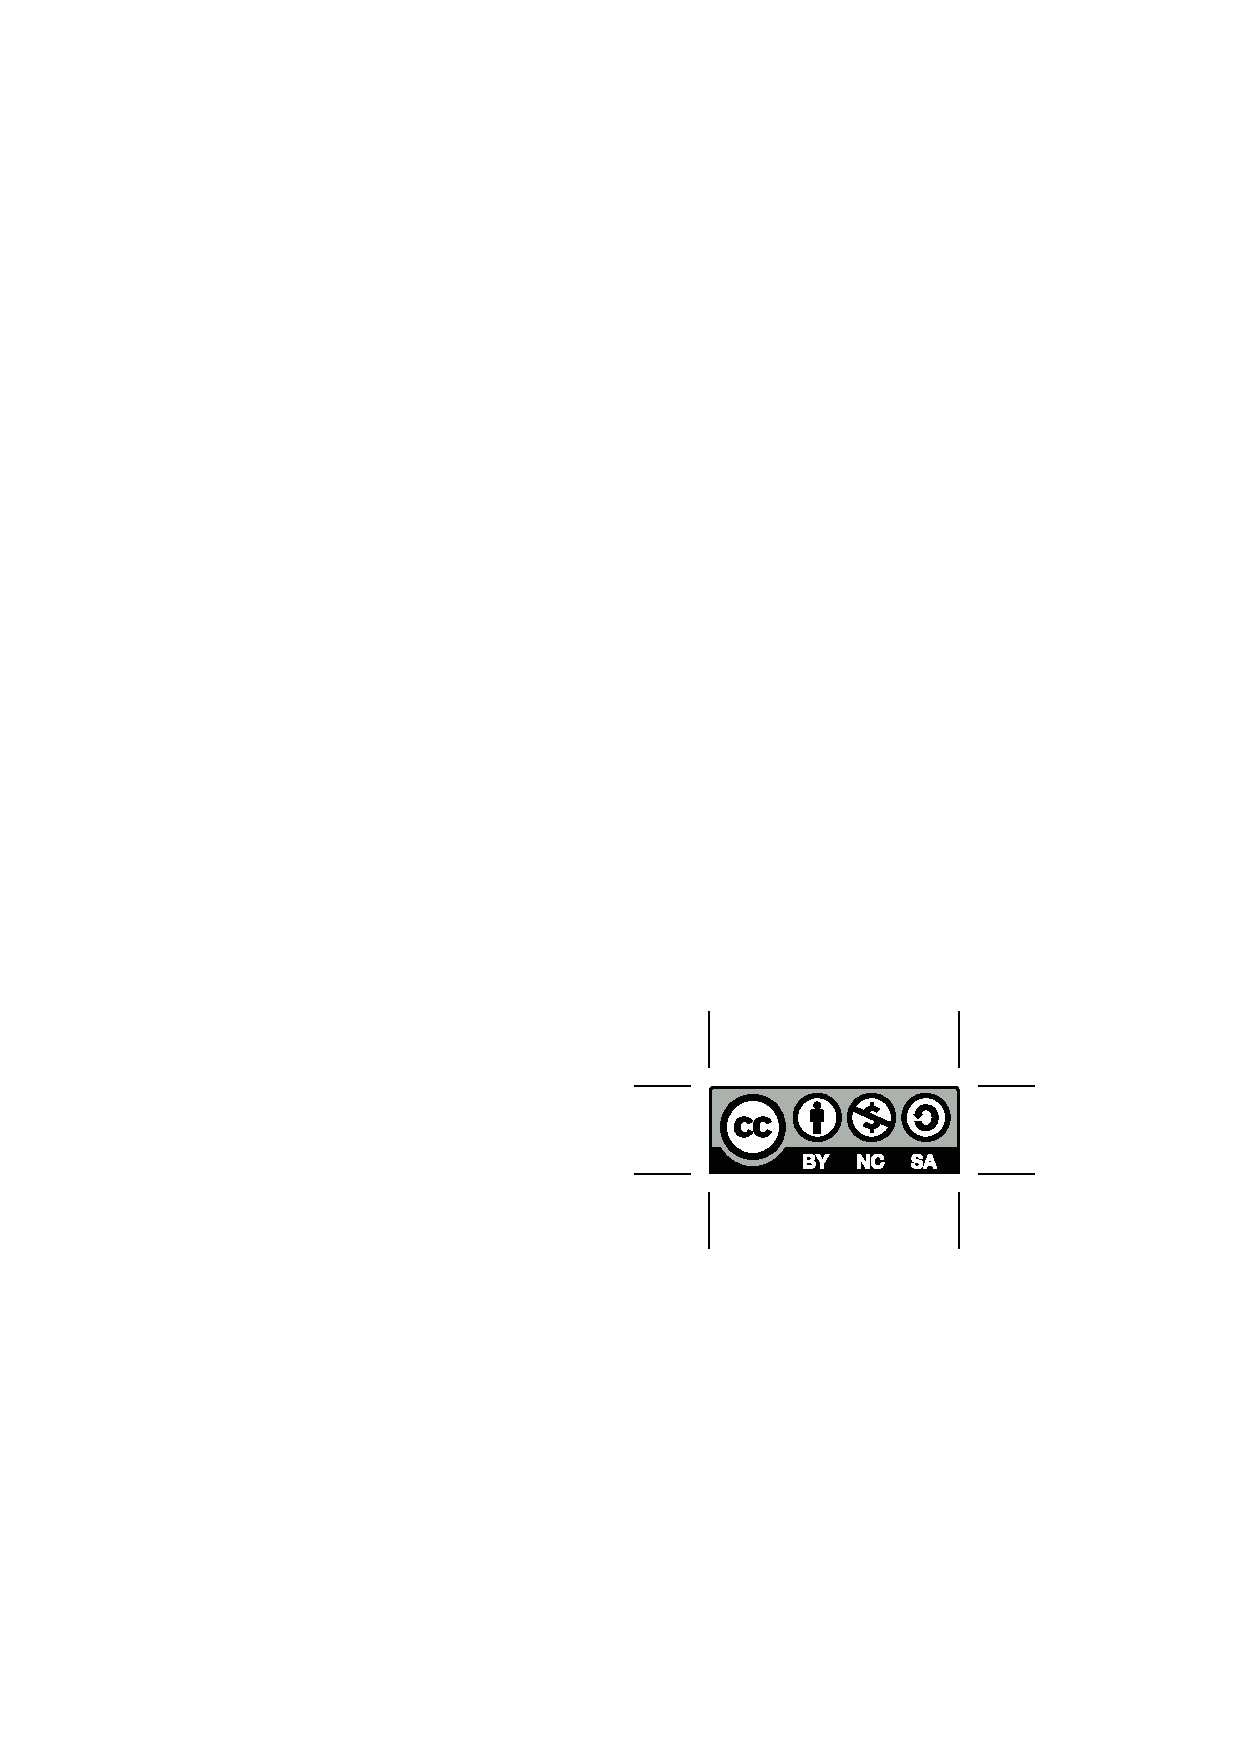
\includegraphics[width=1.38in]{figures/license}
\quad

\includegraphics[width=1.38in]{figures/license2}
%\end{floatingfigure}

\bigskip

\noindent
This work
%PRINT
% not for lulu
%(except the cover art)
is dual licensed under
the Creative Commons
Attribution-Non\-commercial-Share Alike 4.0 International License and
the Creative Commons
Attribution-Share Alike 4.0 International License.
To view a
copy of these licenses, visit
\url{https://creativecommons.org/licenses/by-nc-sa/4.0/}
or
\url{https://creativecommons.org/licenses/by-sa/4.0/}
or send a letter to
Creative Commons
PO Box 1866, Mountain View, CA 94042, USA\@.
%Creative Commons, 171 Second Street, Suite 300, San Francisco, California,
%94105, USA.

\bigskip

\noindent
You can use, print, duplicate, and share this book as much as you want.  You can
base your own notes on it and reuse parts if you keep the license the
same.  You can assume the license is either CC-BY-NC-SA or CC-BY-SA\@,
whichever is compatible with what you wish to do.
Your derivative work must use at least one of the licenses.
Derivative works must be prominently marked as such.
%If you plan to use it commercially (sell it for more than just
%duplicating cost), then you need to contact me and we will work something out.
%If you are printing a course pack for your students, then it is fine if the 
%duplication service is charging a fee for printing and selling the printed
%copy.  I consider that duplicating cost.

\bigskip

\noindent
During the writing of this book, 
the author was in part supported by NSF grant DMS-0900885 and
DMS-1362337.

\bigskip

\noindent
The date is the main identifier of version.  The major version / edition
number is raised only if there have been substantial changes.
%, if only
%very minor changes or fixes are done only the minor version is raised.
Edition
number started at 5, that is, version 5.0, as it was not kept track of
before.
%The Createspace edition ISBN number identifies the major version, and is not
%changed for minor updates fixing errata.
%The edition given with the ISBN number is the major version.

\bigskip

\noindent
See \url{https://www.jirka.org/diffyqs/} for more information
(including contact information).

\bigskip

\noindent
The \LaTeX\ source for the book is available
for possible modification and customization
at github: \url{https://github.com/jirilebl/diffyqs}
\end{small}

\diffytableofcontents

\newpage

%mbxENDIGNORE

%mbx <!--HERE IS WHERE WE ADD MBX PREAMBLE AFTER book-->
%mbx <!--HERE IS WHERE WE ADD MBX PREAMBLE 2-->

%%%%%%%%%%%%%%%%%%%%%%%%%%%%%%%%%%%%%%%%%%%%%%%%%%%%%%%%%%%%%%%%%%%%%%%%%%%%%%

% Introduction chapter
\chapter*{Introduction} \label{intro:chapter}
%mbxSTARTIGNORE
\addfakecontentsline{Introduction}
\markboth{INTRODUCTION}{INTRODUCTION}
%mbxENDIGNORE

%%%%%%%%%%%%%%%%%%%%%%%%%%%%%%%%%%%%%%%%%%%%%%%%%%%%%%%%%%%%%%%%%%%%%%%%%%%%%%

\section{Notes about these notes}
\label{notes:section}

\sectionnotes{A section for the instructor.}

This book originated from my class notes for Math 286
at the \href{https://www.math.uiuc.edu/}{University of Illinois at
Urbana-Champaign} (UIUC)
in Fall 2008 and
Spring 2009.
It is a first course on differential equations for engineers.
Using this book, I also taught Math 285 at UIUC\@,
Math 20D at
\href{https://www.math.ucsd.edu/}{University of California, San Diego} (UCSD),
and Math 4233 at 
\href{https://math.okstate.edu/}{Oklahoma State University} (OSU).
Normally these courses are taught with
Edwards and Penney, \emph{Differential
Equations and Boundary Value Problems: Computing and Modeling}~\cite{EP}, or
Boyce and DiPrima's
\emph{Elementary
Differential Equations and Boundary Value Problems}~\cite{BD},
and this book aims to be more or less a drop-in replacement.
Other books I used as sources of information and inspiration
are E.L.\ Ince's classic (and inexpensive)
\emph{Ordinary Differential Equations}~\cite{I},
Stanley Farlow's \emph{Differential Equations and Their
Applications}~\cite{F}, now available from Dover,
Berg and McGregor's
\emph{Elementary Partial Differential Equations}~\cite{BM},
and William Trench's free book
\emph{Elementary
Differential Equations with Boundary Value Problems}~\cite{T}.
See the \hyperref[furtherreading:chapter]{Further Reading} chapter at the end of the book.

\subsection{Organization}

The organization of this book to some degree
requires chapters be done in order.
Later chapters can be dropped.
The dependence of the material covered is roughly:

% If changing make sure to also update figures/chapterdiagram.pdf_t
% That's a hopefully short term hack before I figure out how to do it
% better so that it also gets links and such
%mbxSTARTIGNORE
\begin{equation*}
\begin{tikzcd}[cramped, row sep=small]
& {\text{\hyperref[intro:chapter]{Introduction}}} \arrow[d] \\
{\text{\Appendixref{linalg:appendix}}} \arrow[dd, dotted]
& {\text{\Chapterref{fo:chapter}}} \arrow[d] \\
& {\text{\Chapterref{ho:chapter}}} \arrow[dddr] \arrow[dd] \arrow[dl] \arrow[dr] \\
{\text{\Chapterref{sys:chapter}}} \arrow[dr, dotted] \arrow[d] & &
  {\text{\Chapterref{ps:chapter}}} \\
{\text{\Chapterref{nlin:chapter}}} & {\text{\Chapterref{FS:chapter}}} \arrow[d]
\arrow[dr,dotted] \\
& {\text{\Chapterref{SL:chapter}}}
& {\text{\Chapterref{LT:chapter}}}
\end{tikzcd}
\end{equation*}
%mbxENDIGNORE
%mbxlatex \begin{center}
%mbxlatex \inputpdft{chapterdiagram}
%mbxlatex \end{center}

There are a few references in chapters \ref{FS:chapter} and \ref{SL:chapter}
to \chapterref{sys:chapter} (some linear algebra), but these
references are not essential and can be skimmed over,
so \chapterref{sys:chapter}
can safely be dropped, while still covering
chapters \ref{FS:chapter} and \ref{SL:chapter}.
\Chapterref{LT:chapter} does not depend on 
\chapterref{FS:chapter} except that the
PDE section \ref{laplacepde:section} makes a
few references to
\chapterref{FS:chapter},
although it could in theory be covered
separately.
The more in-depth \appendixref{linalg:appendix} on linear algebra
can replace the short review \sectionref{sec:matrix}
for a course that combines linear algebra and ODE\@.

%\medskip
\subsection{Typical types of courses}

Several typical types of courses can be run with the book.
There are the two original courses at UIUC\@,
both cover ODE as well some PDE\@.
Either, there is the 4 hours-a-week for a semester (Math 286 at UIUC):

\medskip

\noindent
\hyperref[intro:chapter]{Intro.} (\ref{introde:section}),
\chapterref{fo:chapter} (\ref{integralsols:section}--\ref{numer:section}),
\chapterref{ho:chapter},
\chapterref{sys:chapter},
\chapterref{FS:chapter} (\ref{bvp:section}--\ref{dirich:section}),
\chapterref{SL:chapter} (or
\ref{LT:chapter} or \ref{ps:chapter} or \ref{nlin:chapter}).

\medskip

Or, the second course at UIUC is at 3 hours-a-week (Math 285 at UIUC):

\medskip

\noindent
\hyperref[intro:chapter]{Intro.} (\ref{introde:section}),
\chapterref{fo:chapter} (\ref{integralsols:section}--\ref{numer:section}),
\chapterref{ho:chapter},
\chapterref{FS:chapter} (\ref{bvp:section}--\ref{dirich:section}),
(and maybe \chapterref{SL:chapter},
\ref{LT:chapter}, or \ref{ps:chapter}).

\medskip

A semester course at 3 hours a week that doesn't cover either systems or PDE
will cover, beyond the introduction,
%\sectionref{introde:section},
\chapterref{fo:chapter},
\chapterref{ho:chapter},
\chapterref{LT:chapter}, and \chapterref{ps:chapter},
(with sections skipped as above).
On the other hand, a typical course that covers 
systems will probably need to skip Laplace and power series
and cover
%\sectionref{introde:section},
\chapterref{fo:chapter},
\chapterref{ho:chapter},
\chapterref{sys:chapter}, and \chapterref{nlin:chapter}.

\medskip

If sections need to be skipped in the beginning, a good core of the 
sections on single ODE is:
\ref{introde:section},
\ref{integralsols:section}--\ref{intfactor:section},
\ref{auteq:section},
\ref{solinear:section},
\ref{sec:ccsol},
\ref{sec:mv}--\ref{forcedo:section}.

\medskip

The complete book can be covered at a reasonably
fast pace at approximately 76 lectures
(without \appendixref{linalg:appendix})
or 86 lectures (with \appendixref{linalg:appendix} replacing
\sectionref{sec:matrix}).
This is not accounting for exams, review,
or time spent in computer lab. % (if using IODE for example).
A two quarter or a two semester course can be easily run with the material.
For example (with some sections perhaps strategically skipped):

\medskip

\noindent
Semester 1:
\hyperref[intro:chapter]{Introduction},
\chapterref{fo:chapter},
\chapterref{ho:chapter},
\chapterref{LT:chapter},
\chapterref{ps:chapter}.
\\
Semester 2: 
\Chapterref{sys:chapter},
\chapterref{nlin:chapter},
\chapterref{FS:chapter},
\chapterref{SL:chapter}.

\medskip

A combined course on ODE with linear algebra can run as:

\medskip

\noindent
\hyperref[intro:chapter]{Introduction},
\chapterref{fo:chapter} (\ref{integralsols:section}--\ref{numer:section}),
\chapterref{ho:chapter},
\appendixref{linalg:appendix},
\chapterref{sys:chapter} (w/o \sectionref{sec:matrix}), (possibly 
\chapterref{nlin:chapter}).

\medskip

The chapter on
Laplace transform (\chapterref{LT:chapter}),
the chapter on Sturm--Liouville (\chapterref{SL:chapter}),
the chapter on power series (\chapterref{ps:chapter}),
and the chapter on nonlinear systems (\chapterref{nlin:chapter}),
are more or less interchangeable, and can be treated as \myquote{topics}.
If \chapterref{nlin:chapter} is covered it may be best to place it right 
after \chapterref{sys:chapter},
and \chapterref{SL:chapter} is best covered right after
\chapterref{FS:chapter}.
If time is short, the first two sections of
\chapterref{ps:chapter} make a reasonable self-contained unit.

%\medskip
\subsection{Computer resources}

The following resources are available at the book
website \url{https://www.jirka.org/diffyqs/}:
\begin{enumerate}
\item Interactive SAGE demos.
\item Online WeBWorK homeworks
(using either your own WeBWorK installation or Edfinity)
for most sections, customized for this book.
\item The PDFs of the figures used in this book.
\end{enumerate}

I taught the UIUC courses using IODE\index{IODE software}
(\url{https://faculty.math.illinois.edu/iode/}).
IODE is a free software package that
works with Matlab (proprietary) or Octave (free software).
%Unfortunately IODE is not kept up to date at this point, and may have
%trouble running on newer versions of Matlab.
The graphs in the book were made with
the Genius\index{Genius software} software
(see \url{https://www.jirka.org/genius.html}).  I use Genius
in class to show these (and other) graphs.

The \LaTeX\ source of the book is also available
for possible modification and customization
at github (\url{https://github.com/jirilebl/diffyqs}).

%\medskip

%\textbf{Acknowlegements:}

\subsection{Acknowledgments}

Firstly, I would like to acknowledge Rick Laugesen.  I used his handwritten
class notes
the first time I taught
Math 286.  My organization of this book through chapter 5,
and the choice of
material covered, is heavily influenced by his notes.  Many
examples and computations are taken from his notes.  I am also heavily
indebted to Rick for all the advice he has given me, not just on teaching
Math 286.
For spotting errors and other suggestions,
I would also like to acknowledge (in no particular order):
John P.\ D'Angelo,
Sean Raleigh, Jessica Robinson, Michael Angelini, Leonardo Gomes, Jeff
Winegar, Ian Simon, Thomas Wicklund, Eliot Brenner, Sean Robinson,
Jannett Susberry, Dana Al-Quadi, Cesar Alvarez, Cem Bagdatlioglu,
Nathan Wong, Alison Shive, Shawn White, Wing Yip Ho, Joanne Shin,
Gladys Cruz, Jonathan Gomez, Janelle Louie, Navid Froutan,
Grace Victorine, Paul Pearson, Jared Teague, Ziad Adwan,
Martin Weilandt, S\"{o}nmez \c{S}ahuto\u{g}lu,
Pete Peterson, Thomas Gresham, Prentiss Hyde, Jai Welch,
Simon Tse, Andrew Browning, James Choi, Dusty Grundmeier,
John Marriott,
Jim Kruidenier,
Barry Conrad,
Wesley Snider,
Colton Koop,
Sarah Morse,
Erik Boczko,
Asif Shakeel,
Chris Peterson,
Nicholas Hu,
Paul Seeburger,
Jonathan McCormick,
David Leep,
and probably others I
have forgotten.
Finally, I would like
to acknowledge NSF grants DMS-0900885 and DMS-1362337.


%%%%%%%%%%%%%%%%%%%%%%%%%%%%%%%%%%%%%%%%%%%%%%%%%%%%%%%%%%%%%%%%%%%%%%%%%%%%%%

\sectionnewpage
\section{Introduction to differential equations}
\label{introde:section}

\sectionnotes{more than 1 lecture\EPref{, \S1.1 in \cite{EP}}\BDref{,
chapter 1 in \cite{BD}}}

\subsection{Differential equations}

The laws of physics are generally written down as differential
equations.  Therefore, all of science and engineering use
differential equations to some degree.  Understanding
differential equations is essential to understanding almost anything you will
study in your science and engineering classes.
You can think of mathematics as the language of science, and
differential equations are one of the most important parts of this
language as far as science and engineering are concerned.  As an analogy,
suppose all your classes from now on were given in Swahili.  
It would be important to first learn Swahili, or you would have a very
tough time getting a good grade in your classes.

You saw many
differential equations already without perhaps knowing about it.
And you even solved simple
differential equations when you took calculus.
Let us see an example you may not have seen:
\begin{equation} \label{eq1}
\frac{dx}{dt} + x = 2 \cos t .
\end{equation}
Here $x$ is the \emph{\myindex{dependent variable}} and $t$ is the
\emph{\myindex{independent variable}}.
Equation \eqref{eq1}
is a basic example of a \emph{\myindex{differential equation}}.  In fact, it
is an example of a \emph{\myindex{first order differential equation}}, since
it involves only the first derivative of the dependent variable.  This 
equation arises from Newton's law of cooling where the ambient
temperature oscillates with time.

\subsection{Solutions of differential equations}

Solving the differential equation means finding $x$ in terms of $t$.  That
is, we want to find a function of $t$, which we call $x$, such that when
we plug $x$, $t$, and $\frac{dx}{dt}$ into \eqref{eq1}, the equation holds.
It is
the same idea as it would be for a normal (algebraic) equation of just
$x$ and $t$.  We claim that
\begin{equation*}
x = x(t) = \cos t + \sin t
\end{equation*}
is a \emph{\myindex{solution}}.
How do we check?  We simply plug $x$ into equation \eqref{eq1}!  First we
need to compute $\frac{dx}{dt}$.  We find that $\frac{dx}{dt} = 
-\sin t + \cos t$.  Now let us compute the left-hand side
of \eqref{eq1}.
\begin{equation*}
\frac{dx}{dt} + x = 
\underbrace{(-\sin t + \cos t)}_{\frac{dx}{dt}}
+
\underbrace{(\cos t + \sin t)}_{x}
=
2\cos t .
\end{equation*}
Yay!  We got precisely the right-hand side.
But there is more!
We claim
$x = \cos t + \sin t + e^{-t}$ is also
a solution.  Let us try,
\begin{equation*}
\frac{dx}{dt} = -\sin t + \cos t - e^{-t} .
\end{equation*}
Again plugging into the left-hand side of \eqref{eq1}
\begin{equation*}
\frac{dx}{dt} + x = 
(-\sin t + \cos t - e^{-t}) +
(\cos t + \sin t + e^{-t})
= 2\cos t .
\end{equation*}
And it works yet again!

So there can be many different solutions.  For this equation all
solutions can be written in the form
\begin{equation*}
x = \cos t + \sin t + C e^{-t} ,
\end{equation*}
for some constant $C$.  See \figurevref{intro:plotsfig} for the graph of a
few of these solutions. 
We will see how we find these solutions
a few lectures from now.

\medskip

\begin{mywrapfig}{3.25in}
\capstart
\diffyincludegraphics{width=3in}{width=4.5in}{intro-plots-alt}
\caption{Few solutions of $\frac{dx}{dt} + x = 2 \cos t$.\label{intro:plotsfig}}
\end{mywrapfig}%


Solving differential equations can be quite hard.  
There is no general method that solves every differential equation.  We will
generally focus on how to get exact formulas for solutions of certain
differential
equations, but we will also spend a little bit of time
on getting approximate solutions.
And we will spend some time on understanding the equations without solving
them.

Most of this book is dedicated to
\emph{ordinary differential equations\index{ordinary differential equation}}
or ODEs\index{ODE}, that is, equations with
only one independent variable, where derivatives are only with respect to
this one variable.
If there are several independent variables, we get
\emph{partial differential equations\index{partial differential equation}}
or PDEs\index{PDE}.
%We will briefly see these near the
%end of the course.

Even for ODEs, which are very well understood, it is not a simple question
of turning a crank to get answers.  
It is important to
know when it is easy to find solutions and how to do so.
Although in real applications you will
leave much of the actual calculations to computers, you
need to understand what they are doing.  It is often necessary
to simplify or transform your equations into something that a computer can
understand and solve.
You may need to make certain assumptions and changes in your
model to achieve this.

To be a successful engineer or scientist, you will be required to solve
problems in your job that you never saw before.  It is important to
learn problem solving techniques, so that you may apply those techniques to
new problems.  A common mistake is to expect to learn some prescription for
solving all the problems you will encounter in your later career.  This
course is no exception.


\subsection{Differential equations in practice}

\begin{mywrapfigsimp}{3.05in}{3.35in}
\noindent
\inputpdft{1-1-fig}
\end{mywrapfigsimp}
So how do we use differential equations in science and engineering?  
First, we have some \emph{\myindex{real-world problem}} we wish
to understand.
We make some simplifying assumptions and create a
\emph{\myindex{mathematical model}}.
That is, we translate the real-world situation into a
set of differential equations.
Then we apply mathematics to get some sort of a
\emph{\myindex{mathematical solution}}.
There is still something left to do.  We have to interpret the results.
We have to figure out what the mathematical solution says about the real-world
problem we started with.

Learning how to formulate the mathematical model and how to interpret the
results is what your physics and engineering classes do.  In this
course we will focus mostly on the mathematical analysis.  Sometimes we will
work with simple real-world examples, so that we have some intuition and
motivation about what we are doing.

Let us look at 
an example of this process.
One of the most basic differential equations
is the standard \emph{\myindex{exponential growth model}}.
Let $P$ denote the population 
of some bacteria on a Petri dish.  We assume that there is enough food
and enough space.  Then the rate of growth of bacteria is proportional
to the population---a large population grows quicker.  Let $t$ denote
time (say in seconds) and $P$ the population.  Our model
is
\begin{equation*}
\frac{dP}{dt} = kP ,
\end{equation*}
for some positive constant $k > 0$.

\begin{example}
Suppose there are 100 bacteria at time 0 and 200 bacteria 10 seconds later.
How many bacteria will there be 1 minute from time 0 (in 60 seconds)?

%mbxSTARTIGNORE
\begin{mywrapfig}{3.25in}
\capstart
\diffyincludegraphics{width=3in}{width=4.5in}{intro-plotbact}
\caption{Bacteria growth in the first 60 seconds.\label{intro:plotbactfig}}
\end{mywrapfig}
%mbxENDIGNORE
%
% Make sure to keep the above and the mbx figure below in sync!
%
First we need to solve the equation.  We claim that a solution is given by
\begin{equation*}
P(t) = C e^{kt} ,
\end{equation*}
where $C$ is a constant.  Let us try:
\begin{equation*}
\frac{dP}{dt} = C k e^{kt} = k P .
\end{equation*}
And it really is a solution.

OK\@, now what?  We do not know $C$, and we do not know $k$.  But we know
something.  We know $P(0) = 100$, and we know 
$P(10) = 200$.  Let us plug these conditions in and see what happens.
\begin{align*}
& 100 = P(0) = C e^{k0} = C ,\\
& 200 = P(10) = 100 \, e^{k10} .
\end{align*}
Therefore, $2 = e^{10k}$ or $\frac{\ln 2}{10} = k \approx 0.069$.
So 
\begin{equation*}
P(t) = 100 \, e^{(\ln 2) t / 10} \approx 100 \, e^{0.069 t} .
\end{equation*}
At one minute, $t=60$, the population is $P(60) = 6400$.  See
\figurevref{intro:plotbactfig}.


%mbxlatex \begin{myfig}
%mbxlatex \capstart
%mbxlatex \diffyincludegraphics{width=3in}{width=4.5in}{intro-plotbact}
%mbxlatex \caption{Bacteria growth in the first 60 seconds.\label{intro:plotbactfig}}
%mbxlatex \end{myfig}


Let us talk about the interpretation of the results.  Does our solution
mean that
there must be exactly 6400 bacteria on the plate at 60s?  No!  We made
assumptions that might not be true exactly, just approximately.
If our assumptions are reasonable,
then there will be approximately 6400 bacteria.
Also, in real life $P$ is a
discrete quantity, not a real number.  However, our model has no problem saying
that for example at 61 seconds, $P(61) \approx 6859.35$.
%Obviously there 
%are either 6859 bacteria or 6860 bacteria.
\end{example}

Normally, the $k$ in $P' = kP$ is known,
and we want to solve
the equation for different \emph{initial conditions\index{initial condition}}.
What does that mean?
Take $k=1$ for simplicity.  Suppose we want to solve the equation
$\frac{dP}{dt} = P$ 
subject to $P(0) = 1000$ (the initial condition).
Then the solution turns out to be (exercise)
\begin{equation*}
P(t) = 1000 \, e^t .
\end{equation*}

We call $P(t) = C e^t$ \emph{the \myindex{general solution}},
as every solution
of the equation can be written in this form for some constant $C$.  We
need an initial condition to find out what $C$ is, in order to find the
\emph{\myindex{particular solution}} we are looking for.  Generally, when we say
\myquote{particular solution,} we just mean some solution.

\subsection{Four fundamental equations} \label{subsection:fourfundamental}

A few equations appear often and
it is useful to just memorize what
their solutions are.
Let us call them the \myindex{four fundamental equations}.
Their solutions
are reasonably easy
to guess by recalling properties of exponentials, sines, and cosines.
They are also simple to check, which is something that you should always do.
No need to wonder if you remembered the solution correctly.

\medskip

First such equation is
\begin{equation*}
\frac{dy}{dx} = k y ,
\end{equation*}
for some constant $k > 0$.
Here $y$ is the dependent and $x$ the independent variable.
The general solution for this equation is
\begin{equation*}
y(x) = C e^{kx} .
\end{equation*}
We saw above that this function is a solution, although we used different
variable names.

\medskip

Next,
\begin{equation*}
\frac{dy}{dx} = -k y ,
\end{equation*}
for some constant $k > 0$.
The general solution for this equation is
\begin{equation*}
y(x) = C e^{-kx} .
\end{equation*}

\begin{exercise}
Check that the $y$ given is really a solution to the equation.
\end{exercise}

Next, take the
\emph{\myindex{second order differential equation}}
\begin{equation*}
\frac{d^2y}{{dx}^2} = -k^2 y ,
\end{equation*}
for some constant $k > 0$.
The general solution for this equation is
\begin{equation*}
y(x) = C_1 \cos(kx) + C_2 \sin(kx) .
\end{equation*}
Since the equation is a second order differential equation,
we have two constants in our general solution.

\begin{exercise}
Check that the $y$ given is really a solution to the equation.
\end{exercise}

Finally, consider the second order differential equation
\begin{equation*}
\frac{d^2y}{{dx}^2} = k^2 y ,
\end{equation*}
for some constant $k > 0$.
The general solution for this equation is
\begin{equation*}
y(x) = C_1 e^{kx} + C_2 e^{-kx} ,
\end{equation*}
or
\begin{equation*}
y(x) = D_1 \cosh(kx) + D_2 \sinh(kx) .
\end{equation*}

For those that do not know, $\cosh$ and $\sinh$ are defined by
\begin{equation*}
\cosh x = \frac{e^{x} + e^{-x}}{2} , \qquad
\sinh x = \frac{e^{x} - e^{-x}}{2} .
\end{equation*}
They are called the
\emph{\myindex{hyperbolic cosine}}
and
\emph{\myindex{hyperbolic sine}}.
These functions are sometimes easier to
work with than exponentials.  They have some nice familiar
properties such as
$\cosh 0 = 1$, $\sinh 0 = 0$, and $\frac{d}{dx} \cosh x = \sinh x$ (no that is
not a typo)
and $\frac{d}{dx} \sinh x = \cosh x$.

\begin{exercise}
Check that both forms of the $y$ given are
really solutions to the equation.
\end{exercise}

An interesting note about $\cosh$:  The graph of $\cosh$ is the exact shape
of a hanging chain.  This shape is called
a \emph{\myindex{catenary}}.
Contrary to popular belief this is not a
parabola.  If you invert the graph of $\cosh$ it is also the ideal arch for
supporting its own weight.
For example, the gateway arch in Saint Louis is an inverted graph of
$\cosh$---if it were just a parabola it might fall down.  The formula
used in the design is
inscribed inside the arch:
\begin{equation*}
y = -127.7 \; \textrm{ft} \cdot \cosh({x / 127.7  \; \textrm{ft}}) + 757.7 \;
\textrm{ft} .
\end{equation*}


\subsection{Exercises}

\begin{exercise}
Show that $x = e^{4t}$ is a solution to $x'''-12 x'' + 48 x' - 64 x = 0$.
\end{exercise}

\begin{exercise}
Show that $x = e^{t}$ is not a solution to $x'''-12 x'' + 48 x' - 64 x = 0$.
\end{exercise}

\begin{exercise}
Is $y = \sin t$ a solution to ${\left( \frac{dy}{dt} \right)}^2 = 1 - y^2$?
Justify.
\end{exercise}

\begin{exercise}
Let $y'' + 2y' - 8y = 0$.  Now try a solution of the form $y = e^{rx}$ for
some (unknown) constant $r$.  Is this a solution
for some $r$?  If so, find all such $r$.
\end{exercise}

\begin{exercise}
Verify that $x = C e^{-2t}$ is a solution to $x' = -2x$.
Find $C$ to solve for the initial condition $x(0) = 100$.
\end{exercise}

\begin{exercise}
Verify that $x = C_1 e^{-t} + C_2 e^{2t}$ is a solution to $x'' - x' -2 x =
0$.  Find $C_1$ and $C_2$ to solve for the initial conditions $x(0) = 10$
and $x'(0) = 0$.
\end{exercise}

\begin{exercise}
Find a solution to
${(x')}^2 + x^2 = 4$
using your knowledge of derivatives of functions that you
know from basic calculus.
\end{exercise}

\begin{exercise}
\pagebreak[2]
Solve:
\begin{tasks}(2)
\task $\dfrac{dA}{dt} = -10 A, \quad A(0)=5$
\task $\dfrac{dH}{dx} = 3 H, \quad H(0)=1$
\task $\dfrac{d^2y}{dx^2} = 4 y, \quad y(0)=0, \quad y'(0)=1$
\task $\dfrac{d^2x}{dy^2} = -9 x, \quad x(0)=1, \quad x'(0)=0$
\end{tasks}
\end{exercise}

\begin{exercise}
Is there a solution to $y' = y$, such that $y(0) = y(1)$?
\end{exercise}

%mbxSTARTIGNORE
\noindent
\emph{Note: Exercises with numbers 101 and higher have solutions in the
back of the book.}
%mbxENDIGNORE

%mbx <p><em>Note: Exercises with numbers 101 and higher have solutions.</em></p>

\setcounter{exercise}{100}

\begin{exercise}
Show that $x = e^{-2t}$ is a solution to $x'' + 4x' + 4x = 0$.
\end{exercise}
\exsol{%
Compute $x' = -2e^{-2t}$ and $x'' = 4e^{-2t}$.  Then
$(4e^{-2t}) + 4 (-2e^{-2t}) + 4 (e^{-2t}) = 0$.
}

\begin{exercise}
Is $y = x^2$ a solution to $x^2y'' - 2y = 0$?  Justify.
\end{exercise}
\exsol{%
Yes.
}

\begin{exercise}
Let $xy'' - y' = 0$.  Try a solution of the form $y = x^r$.  Is this a
solution for some $r$?  If so, find all such $r$.
\end{exercise}
\exsol{%
$y=x^r$ is a solution for $r=0$ and $r=2$.
}


\begin{exercise}
Verify that $x=C_1e^t+C_2$ is a solution to $x''-x' = 0$.  Find $C_1$ and
$C_2$ so that $x$ satisfies $x(0) = 10$ and $x'(0) = 100$.
\end{exercise}
\exsol{%
$C_1 = 100$, $C_2 = -90$
}

\begin{exercise}
Solve $\frac{d\varphi}{ds} = 8 \varphi$ and $\varphi(0) = -9$.
\end{exercise}
\exsol{%
$\varphi = -9 e^{8s}$
}

%%%%%%%%%%%%%%%%%%%%%%%%%%%%%%%%%%%%%%%%%%%%%%%%%%%%%%%%%%%%%%%%%%%%%%%%%%%%%%

\sectionnewpage
\section{Classification of differential equations}
\label{classification:section}

%Perhaps no [EP] ref?
\sectionnotes{less than 1 lecture or left as reading\BDref{, \S1.3 in \cite{BD}}}

There are many types of differential equations, and we classify them into
different categories based on their properties.  Let us quickly go over
the most basic classification.  We already saw the distinction
between ordinary and partial differential equations:
\begin{itemize}
\item
\emph{Ordinary differential equations}
\index{Ordinary differential equations}\index{ODE} or (ODE) are
equations where the derivatives are taken with respect to only one variable.
That is, there is only one independent variable.
\item
\emph{Partial differential equations}
\index{Partial differential equations}\index{PDE} or (PDE) are
equations that depend on partial derivatives of several variables.
That is, there are several independent variables.
\end{itemize}

Let us see some examples of ordinary differential equations:
\begin{align*}
& \frac{d y}{dt} = ky , & & \text{(Exponential growth\index{exponential growth})} \\
& \frac{d y}{dt} = k(A-y) , & & \text{(\myindex{Newton's law of cooling})} \\
& m \frac{d^2 x}{dt^2} + c \frac{dx}{dt} + kx = f(t) . & &
\text{(Mechanical vibrations\index{mechanical vibrations})}
\end{align*}
And of partial differential equations:
\begin{align*}
& \frac{\partial y}{\partial t} + c \frac{\partial y}{\partial x} = 0 , & & 
\text{(Transport equation\index{transport equation})} \\
& \frac{\partial u}{\partial t} = \frac{\partial^2 u}{\partial x^2} , & & 
\text{(Heat equation\index{heat equation})} \\
& \frac{\partial^2 u}{\partial t^2} = \frac{\partial^2 u}{\partial x^2} +
\frac{\partial^2 u}{\partial y^2} . & & 
\text{(Wave equation in 2 dimensions\index{wave equation in 2 dimensions})}
\end{align*}

If there are several equations working together we have a so-called
\emph{\myindex{system of differential equations}}.  For example,
\begin{equation*}
y' = x , \qquad x' = y
\end{equation*}
is a simple system of ordinary differential equations.
\myindex{Maxwell's equations} for electromagnetics,
\begin{align*}
& \nabla \cdot \vec{D} = \rho, & & \nabla \cdot \vec{B} = 0 , \\
& \nabla \times \vec{E} = - \frac{\partial \vec{B}}{\partial t}, &
& \nabla \times \vec{H} = \vec{J} + \frac{\partial \vec{D}}{\partial t} ,
\end{align*}
are a system of partial differential equations. 
The divergence operator $\nabla \cdot$ and the
curl operator $\nabla \times$ can be written out in partial derivatives of
the functions involved in the $x$, $y$, and $z$ variables.

\medskip

The next bit of information is the \emph{\myindex{order}} of the
equation (or system).  The order is simply the order of the largest
derivative that appears.  If the highest derivative that appears is
the first derivative, the equation is of first order.  If the highest
derivative that appears is the second derivative, then the equation is of second
order.  For example, Newton's law of cooling above is a first order
equation, while the mechanical vibrations equation is a second order equation.
The equation governing transversal vibrations in a beam,
\begin{equation*}
a^4 \frac{\partial^4 y}{\partial x^4} + \frac{\partial^2 y}{\partial t^2} = 0,
\end{equation*}
is a fourth order partial differential equation.  It is
fourth order since at least one derivative is the fourth derivative.  It
does not matter that derivatives with respect to $t$ are only second order.

In the first chapter we will start attacking first order ordinary
differential equations, that is, equations of the form $\frac{dy}{dx} = f(x,y)$.
In general, lower order equations are easier to work with and have simpler
behavior, which is why we start with them.

\medskip

We also distinguish how the dependent variables appear in the equation (or
system).  In particular, we say an equation is
\emph{linear}\index{linear equation} if the
dependent variable (or variables) and their derivatives appear linearly,
that is only as first powers, they are not multiplied together, and no other functions of the dependent
variables appear.  In other words, the equation is a sum of terms,
where each term is
some function of the independent variables
or 
some function of the independent variables
multiplied by a dependent variable
or its derivative.
Otherwise, the equation is called
\emph{nonlinear}\index{nonlinear equation}.
For example,
an ordinary differential equation is linear if it can be
put into the form
\begin{equation} \label{classification:eqlingen}
a_n(x) \frac{d^n y}{dx^n} + 
a_{n-1}(x) \frac{d^{n-1} y}{dx^{n-1}} + 
\cdots
+
a_{1}(x) \frac{dy}{dx}
+
a_{0}(x) y = b(x) .
\end{equation}
The functions $a_0$, $a_1$, \ldots, $a_n$ are called the
\emph{\myindex{coefficients}}.
The equation is allowed to depend arbitrarily on the independent variable.
So 
\begin{equation} \label{classification:eqlinex}
e^x \frac{d^2 y}{dx^2} + 
\sin(x) \frac{d y}{dx} + 
x^2 y
=
\frac{1}{x}
\end{equation}
is still a linear equation as $y$ and its derivatives only appear linearly.

All the equations and systems given above as examples are linear.  
It may not be immediately obvious for Maxwell's equations unless you write out
the divergence and curl in terms of partial derivatives.  Let us see some
nonlinear equations.  For example \myindex{Burger's equation},
\begin{equation*}
\frac{\partial y}{\partial t} + 
y \frac{\partial y}{\partial x} =
\nu \frac{\partial^2 y}{\partial x^2} ,
\end{equation*}
is a nonlinear second order partial differential equation.  It is nonlinear
because $y$ and $\frac{\partial y}{\partial x}$ are multiplied together.
The equation
\begin{equation} \label{classification:eqnonlinode}
\frac{dx}{dt} = x^2
\end{equation}
is a nonlinear first order differential equation as there is a power of
the dependent variable $x$.

\medskip

A linear equation may further be called \emph{\myindex{homogeneous}}, if
all terms depend on the dependent variable.  That is, if there is no
term that is a function of the independent variables alone.  Otherwise, the
equation is called \emph{\myindex{nonhomogeneous}} or
\emph{\myindex{inhomogeneous}}.  For example,
the exponential growth equation, the wave equation, or the transport equation above
are homogeneous. The mechanical vibrations equation above is nonhomogeneous
as long as $f(t)$ is not the zero function.  Similarly, if the ambient temperature $A$ is nonzero,
Newton's law of cooling is nonhomogeneous.
A homogeneous linear ODE can be put into the form
\begin{equation*}
a_n(x) \frac{d^n y}{dx^n} + 
a_{n-1}(x) \frac{d^{n-1} y}{dx^{n-1}} + 
\cdots
+
a_{1}(x) \frac{dy}{dx}
+
a_{0}(x) y = 0 .
\end{equation*}
Compare to \eqref{classification:eqlingen} and notice there is no
function $b(x)$.

\medskip

If the coefficients of a linear equation are actually constant functions,
then the equation is said to have
\emph{constant coefficients}\index{constant coefficient}.
The coefficients are the functions multiplying the dependent
variable(s) or one of its derivatives, not the function $b(x)$ standing alone.
That is,
\begin{equation*}
a_n \frac{d^n y}{dx^n} + 
a_{n-1} \frac{d^{n-1} y}{dx^{n-1}} + 
\cdots
+
a_{1} \frac{dy}{dx}
+
a_{0} y = b(x) ,
\end{equation*}
where $a_0, a_1, \ldots, a_n$ are all constants,
but $b$ may depend on 
the independent variable $x$,
is a constant coefficient nonhomogeneous ODE\@.
The mechanical vibrations equation
above is a constant coefficient nonhomogeneous second order ODE\@.
Same nomenclature applies to PDEs, so the transport equation,
heat equation and wave equation are all examples of constant coefficient
linear PDEs.

\medskip

Finally, an equation (or system) is called \emph{\myindex{autonomous}}
if the equation does not depend on the independent variable.
Usually here we only consider ordinary differential equations and the
independent variable is then thought of as time.  Autonomous equation
means an equation that does not change with time.
For example, Newton's law of cooling is autonomous, so is equation
\eqref{classification:eqnonlinode}.  On the other hand, mechanical
vibrations or 
\eqref{classification:eqlinex} are not autonomous.

\subsection{Exercises}

\begin{exercise}
Classify the following equations.  Are they ODE or PDE\@?  Is it an equation
or a system?  What is the order?  Is it linear or nonlinear, and if it is
linear, is it homogeneous, constant coefficient?  If it is an ODE\@, is it
autonomous?
\begin{tasks}(2)
\task $\displaystyle \sin(t) \frac{d^2 x}{dt^2} + \cos(t) x = t^2$
\task $\displaystyle \frac{\partial u}{\partial x} + 3 \frac{\partial u}{\partial y} = xy$
\task $\displaystyle y''+3y+5x=0, \quad x''+x-y=0$
\task $\displaystyle \frac{\partial^2 u}{\partial t^2} + u\frac{\partial^2 u}{\partial s^2} =
0$
\task $\displaystyle x''+tx^2=t$
\task $\displaystyle \frac{d^4 x}{dt^4} = 0$
\end{tasks}
\end{exercise}

\begin{exercise}
If $\vec{u} = (u_1,u_2,u_3)$ is a vector, we have the divergence
$\nabla \cdot \vec{u} =
\frac{\partial u_1}{\partial x} +
\frac{\partial u_2}{\partial y} +
\frac{\partial u_3}{\partial z}$ and curl
$\nabla \times \vec{u} =
\Bigl(
\frac{\partial u_3}{\partial y} - \frac{\partial u_2}{\partial z} , ~
\frac{\partial u_1}{\partial z} - \frac{\partial u_3}{\partial x} , ~
\frac{\partial u_2}{\partial x} - \frac{\partial u_1}{\partial y} \Bigr)$.
Notice that curl of a vector is still a vector.  Write out Maxwell's
equations in terms of partial derivatives and classify the system.
\end{exercise}

\begin{exercise}
Suppose $F$ is a linear function, that is,
$F(x,y) = ax+by$ for constants $a$ and $b$.  What is the
classification of equations of the form $F(y',y) = 0$.
\end{exercise}

\begin{exercise}
Write down an explicit example of a third order, linear, nonconstant coefficient,
nonautonomous, nonhomogeneous system of two ODE such that every derivative
that could appear, does appear.
\end{exercise}

\setcounter{exercise}{100}

\pagebreak[2]
\begin{exercise}
Classify the following equations.  Are they ODE or PDE\@?  Is it an equation
or a system?  What is the order?  Is it linear or nonlinear, and if it is
linear, is it homogeneous, constant coefficient?  If it is an ODE\@, is it
autonomous?
\begin{tasks}(2)
\task $\displaystyle \frac{\partial^2 v}{\partial x^2} + 3 \frac{\partial^2
v}{\partial y^2} = \sin(x)$
\task $\displaystyle \frac{d x}{dt} + \cos(t) x = t^2+t+1$
\task $\displaystyle \frac{d^7 F}{dx^7} = 3F(x)$
\task $\displaystyle y''+8y'=1$
\task $\displaystyle x''+tyx'=0, \quad y''+txy = 0$
\task $\displaystyle \frac{\partial u}{\partial t} = \frac{\partial^2 u}{\partial s^2} + u^2$
\end{tasks}
\end{exercise}
\exsol{%
a) 
PDE\@, equation, second order, linear, nonhomogeneous, constant coefficient.\\
b) 
ODE\@, equation, first order, linear, nonhomogeneous, not constant coefficient, not autonomous.\\
c) 
ODE\@, equation, seventh order, linear, homogeneous, constant coefficient, autonomous.\\
d) 
ODE\@, equation, second order, linear, nonhomogeneous, constant coefficient, autonomous.\\
e) 
ODE\@, system, second order, nonlinear.\\
f) 
PDE\@, equation, second order, nonlinear.
}

\begin{exercise}
Write down the general \emph{zero}th order linear ordinary differential
equation.  Write down the general solution.
\end{exercise}
\exsol{%
equation: $a(x) y = b(x)$, solution: $y = \frac{b(x)}{a(x)}$.
}



%%%%%%%%%%%%%%%%%%%%%%%%%%%%%%%%%%%%%%%%%%%%%%%%%%%%%%%%%%%%%%%%%%%%%%%%%%%%%%

% First order ODEs chapter
\chapter{First order equations} \label{fo:chapter}

%%%%%%%%%%%%%%%%%%%%%%%%%%%%%%%%%%%%%%%%%%%%%%%%%%%%%%%%%%%%%%%%%%%%%%%%%%%%%%

\section{Integrals as solutions}
\label{integralsols:section}

\sectionnotes{1 lecture (or less)\EPref{, \S1.2 in \cite{EP}}\BDref{,
covered in \S1.2 and \S2.1 in \cite{BD}}}

A first order ODE is an equation of the form
\begin{equation*}
\frac{dy}{dx} = f(x,y) ,
\end{equation*}
or just
\begin{equation*}
y' = f(x,y) .
\end{equation*}
In general, there is no simple formula or procedure one can follow to find
solutions.
In the next few lectures we will look at special cases where solutions are not
difficult to obtain.
In this section, let us assume that $f$ is a function of $x$ alone,
that is, the equation is
\begin{equation} \label{ias:inteq}
y' = f(x) .
\end{equation}
We could just integrate (antidifferentiate) both sides with respect to $x$.
\begin{equation*}
\int y'(x) \,dx = \int f(x) \,dx + C ,
\end{equation*}
that is
\begin{equation*}
y(x) = \int f(x) \,dx + C .
\end{equation*}
This $y(x)$ is actually the general solution.
So to solve \eqref{ias:inteq},
we find some antiderivative of $f(x)$
and then we add an arbitrary constant to get the general solution.

\begin{example}
Find the general solution of $y' = 3 x^2$.

Elementary calculus tells us
that the general solution must be $y = x^3 + C$.  Let us check by
differentiating:
$y' = 3x^2$.  We got \emph{precisely} our equation back.
\end{example}

Now is a good time to discuss a point about
calculus notation and terminology.  Calculus
textbooks muddy the waters by talking about the integral as primarily the
so-called indefinite integral.  The \myindex{indefinite integral}
is really the \emph{\myindex{antiderivative}} 
(in fact the whole one-parameter family
of antiderivatives).  There really exists only one integral and that
is the definite integral.
The only reason for the indefinite integral notation is that we can always
write an antiderivative as a (definite) integral.  That is, by the fundamental
theorem of calculus we can always write
$\int f(x) \,dx + C$ as
\begin{equation*}
\int_{x_0}^x f(t) \,dt + C .
\end{equation*}
Hence the terminology \emph{to \myindex{integrate}} when we may really mean
\emph{to \myindex{antidifferentiate}}.
Integration is just one way to compute the
antiderivative (and it is a way that always works, see the following
examples).  Integration is defined as the area under the graph, it
only happens to also compute antiderivatives.
For sake of consistency, we will keep using the
indefinite integral notation when we want an antiderivative,
and you should \emph{always} think of the definite integral
as a way to write it.

Normally, we also have an initial condition such as $y(x_0) = y_0$
for some two numbers $x_0$ and $y_0$ ($x_0$ is often 0, but not always).
We can then write the solution as a definite integral in a nice way.
Suppose our problem is $y' = f(x)$, $y(x_0) = y_0$.  Then the solution is
\begin{equation} \label{int:eqdef}
y(x) = \int_{x_0}^x f(t) \,dt + y_0 .
\end{equation}
Let us check!
We compute
$y' = f(x)$ via the fundamental theorem of calculus, and by Jupiter, $y$ is a
solution.  Is it the one satisfying the initial condition?  Well,
$y(x_0) = \int_{x_0}^{x_0} f(t)\,dt + y_0 = y_0$.  It is!

Do note that the definite integral and the indefinite integral
(antidifferentiation) are completely different beasts.  The definite integral
always evaluates to a number.  Therefore, \eqref{int:eqdef} is a formula we
can plug into the calculator or a computer, and it will be happy to calculate
specific values for us.  We will easily be able to plot the
solution and work with it just like with any other function.
It is not so crucial to always find a
closed form for the antiderivative.

\begin{example}
Solve
\begin{equation*}
y' = e^{-x^2}, \qquad y(0) = 1 .
\end{equation*}

By the preceding discussion, the solution must be
\begin{equation*}
y(x) = \int_0^x e^{-s^2} \,ds + 1 .
\end{equation*}
Here is a good way to make fun of your friends taking second semester
calculus.  Tell them to
find the closed form solution.  Ha ha ha (bad math joke).  It is
not possible (in closed form).
There is absolutely nothing wrong with writing the solution as a
definite integral.
This particular integral
is in fact very important
in statistics.
\end{example}

Using this method, we can also solve equations of the form
\begin{equation*}
y' = f(y) .
\end{equation*}
Let us write the equation in \myindex{Leibniz notation}.
\begin{equation*}
\frac{dy}{dx} = f(y) .
\end{equation*}
Now we use the inverse function theorem from calculus
to switch the roles of $x$ and $y$
to obtain
\begin{equation*}
\frac{dx}{dy} = \frac{1}{f(y)} .
\end{equation*}
What
we are doing seems like algebra with $dx$ and $dy$.
It is tempting to just do algebra with $dx$
and $dy$ as if they were numbers.  And in this case it does work.  Be
careful,
however, as this sort of hand-waving calculation can lead to trouble,
especially when
more than one independent variable is involved.
At this point, we can simply integrate,
\begin{equation*}
x(y) = \int \frac{1}{f(y)} \,dy + C .
\end{equation*}
Finally, we try to solve for $y$.

\begin{example}
Previously, we guessed $y' = ky$ (for some $k > 0$) has the solution
$y=Ce^{kx}$.  We could have found the solution by integrating.
First we note that $y=0$ is a solution.
Henceforth, we assume $y\not= 0$.  We write
\begin{equation*}
\frac{dx}{dy} = \frac{1}{ky} .
\end{equation*}
We integrate to obtain
\begin{equation*}
x(y) = x = \frac{1}{k} \ln \, \lvert y \rvert + D,
\end{equation*}
where $D$ is an arbitrary constant.
Now we solve for $y$ (actually for $\lvert y \rvert$).
\begin{equation*}
\lvert y \rvert =
e^{kx-kD} = 
e^{-kD} e^{k x} .
\end{equation*}
If we replace $e^{-kD}$ with an arbitrary constant $C$, we can
get rid of the absolute value bars (which we can do as $D$ was arbitrary).  In
this way, we
also incorporate the solution $y=0$.  We get the same general solution as
we guessed before, $y = Ce^{kx}$.
\end{example}

\begin{example}
Find the general solution of
$y' = y^2$.

First we note that $y=0$ is a solution.  We can now assume that $y \not= 0$.
Write
\begin{equation*}
\frac{dx}{dy} = \frac{1}{y^2} .
\end{equation*}
We integrate to get
\begin{equation*}
x = \frac{-1}{y} + C .
\end{equation*}
We solve for $y = \frac{1}{C-x}$.
So the general solution is
\begin{equation*}
y = \frac{1}{C-x} \qquad \text{or} \qquad y = 0.
\end{equation*}
Note the singularities of the solution.  If, for example, $C=1$, then the
solution \myquote{blows up} as we approach $x=1$.  See
\figurevref{1over1mx:fig}.  Generally,
it is hard to tell
from just looking at the equation itself how the solution is going to behave.
The equation $y' = y^2$ is very nice and defined everywhere, but
the solution is only defined on some interval $(-\infty, C)$ or
$(C, \infty)$.  Usually when this happens we only consider one of these
the solution.  For example if we impose a condition $y(0) = 1$, then
the solution is $y=\frac{1}{1-x}$, and we would consider this solution only
for $x$ on the interval $(-\infty,1)$.  In the figure, it is the left side
of the graph.
\begin{myfig}
\capstart
\diffyincludegraphics{width=3in}{width=4.5in}{1over1mx}
\caption{Plot of $y=\frac{1}{1-x}$.\label{1over1mx:fig}}
\end{myfig}
\end{example}

Classical problems leading to differential equations solvable by integration
are problems 
dealing with \myindex{velocity},
\myindex{acceleration} and \myindex{distance}.  You have surely seen these
problems before in your calculus class.

\begin{example}
Suppose a car drives at a speed $e^{t/2}$ meters per second,
where $t$ is time in seconds.
How far did the car get in 2 seconds (starting at $t=0$)?  How far in 10 seconds?

Let $x$ denote the distance the car traveled.
The equation is
\begin{equation*}
x' = e^{t/2} .
\end{equation*}
We just integrate this equation to get that
\begin{equation*}
x(t) = 2 e^{t/2} + C . 
\end{equation*}
We still need to figure out $C$.  We know that when $t=0$, then
$x=0$.  That is, $x(0) = 0$.  So
\begin{equation*}
0 = x(0) = 2e^{0/2} + C = 2 + C .
\end{equation*}
Thus $C = -2$ and 
\begin{equation*}
x(t) = 2 e^{t/2} - 2 .
\end{equation*}
Now we just plug in to get where the car is at 2 and at 10 seconds.
We obtain
\begin{equation*}
x(2) = 2e^{2/2} - 2 \approx 3.44 \text{ meters} ,
\qquad
x(10) = 2e^{10/2} - 2 \approx 294 \text{ meters} .
\end{equation*}
\end{example}

\begin{example}
Suppose that the car accelerates at a rate of $\unitfrac[t^2]{m}{s^2}$.
At time $t=0$ the car is at the 1 meter mark and is traveling at
\unitfrac[10]{m}{s}.  Where is the car at time $t=10$?

Well this is actually a second order problem.  If $x$ is the distance
traveled, then $x'$ is the velocity, and $x''$ is the acceleration.
The equation with initial conditions is
\begin{equation*}
x'' = t^2 , \qquad x(0) = 1 , \qquad x'(0) = 10 .
\end{equation*}
What if we say $x' = v$.  Then we have the problem
\begin{equation*}
v' = t^2, \qquad v(0) = 10 .
\end{equation*}
Once we solve for $v$, we can integrate and find $x$.
\end{example}

\begin{exercise}
Solve for $v$, and then solve for $x$.  Find $x(10)$ to answer the
question.
\end{exercise}

\subsection{Exercises}

\begin{exercise}
Solve $\frac{dy}{dx} = x^2+x$ for $y(1)=3$.
\end{exercise}

\begin{exercise}
Solve $\frac{dy}{dx} = \sin (5x)$ for $y(0)=2$.
\end{exercise}

\begin{exercise}
Solve $\frac{dy}{dx} = \frac{1}{x^2-1}$ for $y(0)=0$.
\end{exercise}

\begin{exercise}
Solve $y' = y^3$ for $y(0)=1$.
\end{exercise}

\begin{exercise}[little harder]
Solve $y' = (y-1)(y+1)$ for $y(0)=3$.
\end{exercise}

\begin{exercise}
Solve $\frac{dy}{dx} = \frac{1}{y+1}$ for $y(0)=0$.
\end{exercise}

\begin{exercise}[harder]
Solve $y'' = \sin x$ for $y(0)=0$, $y'(0) = 2$.
\end{exercise}

\begin{exercise}
A spaceship is traveling at the speed \unitfrac[$2t^2+1$]{km}{s} ($t$ is
time in seconds).  It is pointing directly away from earth and at time $t=0$
it is 1000 kilometers from earth.  How far from earth is it at one minute from
time $t=0$?
\end{exercise}

\begin{exercise}
Solve $\frac{dx}{dt} = \sin(t^2)+t$, $x(0)=20$.  It is OK to leave your
answer as a definite integral.
\end{exercise}

\begin{exercise}
A dropped ball accelerates downwards at a constant rate $9.8$ meters per second
squared.  Set up the differential equation for the height above ground $h$ in meters.
Then supposing $h(0) = 100$ meters, how long does it take for the ball to hit
the ground.
\end{exercise}

\begin{exercise}
Find the general solution of
$y' = e^x$,  and then $y' = e^y$.
\end{exercise}


\setcounter{exercise}{100}

\begin{exercise}
Solve $\frac{dy}{dx} = e^x + x$ and $y(0) = 10$.
\end{exercise}
\exsol{%
$y = e^x + \frac{x^2}{2} + 9$
}

\begin{exercise}
Solve $x' = \frac{1}{x^2}$, $x(1)=1$.
\end{exercise}
\exsol{%
$x = {(3t-2)}^{1/3}$
}

\begin{exercise}
Solve $x' = \frac{1}{\cos(x)}$, $x(0)=\frac{\pi}{4}$.
\end{exercise}
\exsol{%
$x = \sin^{-1} \bigl(t+\nicefrac{1}{\sqrt{2}}\bigr)$
}

\begin{exercise}
Sid is in a car traveling at speed $10t+70$ miles per hour away from Las Vegas,
where $t$ is in hours.  At $t=0$, Sid is 10 miles away from Vegas.  How
far from Vegas is Sid 2 hours later?
\end{exercise}
\exsol{%
170
}

\begin{exercise}
Solve $y' = y^n$, $y(0) = 1$, where $n$ is a positive integer.
Hint: You have to consider different cases.
\end{exercise}
\exsol{%
If $n \not= 1$, then
$y={\bigl((1-n)x+1\bigr)}^{1/(1-n)}$.
If $n=1$, then $y = e^x$.
}

\begin{exercise}
The rate of change of the volume of a snowball that is melting is 
proportional to the surface area of the snowball.  Suppose the
snowball is perfectly spherical.  The volume (in centimeters cubed)
of a ball of radius $r$ centimeters is
$(\nicefrac{4}{3}) \pi r^3$.  The surface area is
$4 \pi r^2$.  Set up the differential equation for how the radius $r$ is changing.
Then, suppose that at time $t=0$ minutes, the radius is 10 centimeters.
After 5 minutes, the radius is 8 centimeters.  At what time $t$ will the 
snowball be completely melted?
\end{exercise}
\exsol{%
The equation is $r' = -C$ for some constant $C$.
The snowball will be completely melted in 25 minutes from time $t=0$.
}

\begin{exercise}
Find the general solution to $y''''= 0$.  How many distinct constants do you need?
\end{exercise}
\exsol{%
$y = Ax^3 + Bx^2 + Cx + D$, so 4 constants.
}

%%%%%%%%%%%%%%%%%%%%%%%%%%%%%%%%%%%%%%%%%%%%%%%%%%%%%%%%%%%%%%%%%%%%%%%%%%%%%%

\sectionnewpage
\section{Slope fields}
\label{slopefields:section}

\sectionnotes{1 lecture\EPref{, \S1.3 in \cite{EP}}\BDref{,
\S1.1 in \cite{BD}}}

%At this point it may be good to first try the
%Lab I\index{IODE software!Lab I} and/or Project I\index{IODE software!Project I} from the
%IODE website: \url{http://www.math.uiuc.edu/iode/}.
%
%\medskip

As we said, the general first order equation we are studying looks like
\begin{equation*}
y' = f(x,y).
\end{equation*}
A lot of the time, we cannot simply solve these kinds of equations explicitly.
It would be nice if we could at least figure out the shape and behavior of
the solutions, or find approximate solutions.

\subsection{Slope fields}

%As you have seen in IODE Lab I (if you did it),
The equation $y' = f(x,y)$
gives you a slope at each point 
in the
$(x,y)$-plane.  And this is the slope a solution $y(x)$ would have 
at $x$ if its value was $y$.  In other words, $f(x,y)$ is the slope
of a solution whose graph runs through the
point $(x,y)$.  At a point $(x,y)$, we plot a short line
with the slope $f(x,y)$.
For example, if $f(x,y) = xy$, then at point $(2,1.5)$ we draw a
short line of slope $xy = 2 \times 1.5 = 3$.  So, if $y(x)$ is a solution
and $y(2) = 1.5$, then the equation mandates that $y'(2) = 3$.
See \figurevref{1.3:fig0}.

\begin{myfig}
\capstart
\diffyincludegraphics{width=3in}{width=4.5in}{1-3-xysl-one}
\caption{The slope $y'=xy$ at $(2,1.5)$.\label{1.3:fig0}}
\end{myfig}

To get an idea of how solutions behave, we draw such lines at lots
of points in the plane, not just the point $(2,1.5)$.  We would
ideally want to see the slope at every point, but that is
just not possible.  Usually we pick a
grid of points fine enough so that it shows the behavior, but not too
fine so that we can still recognize the individual lines.
We call this picture the \emph{\myindex{slope field}} of the equation.
See \figurevref{1.3:fig1} for the slope field of the equation $y' = xy$.
Usually in practice, one does not do this by hand, but has a computer do the
drawing.

Suppose we are given a specific initial condition $y(x_0) = y_0$.
A solution, that is, the graph of the solution, would be a curve
that follows the slopes we drew.
For a few sample
solutions, see \figurevref{1.3:fig2}.  It is easy to roughly sketch
(or at least imagine)
possible solutions in the slope field, just from looking at the slope field
itself.  You simply sketch a line that roughly fits the little line segments
and goes through your initial condition.

\begin{myfig}
\parbox[t]{3.0in}{
 \capstart
 \diffyincludegraphics{width=3.0in}{width=4.5in}{1-3-xysl}
 \caption{Slope field of $y' = xy$.\label{1.3:fig1}}
}
\quad
\parbox[t]{3.0in}{
 \capstart
 \diffyincludegraphics{width=3.0in}{width=4.5in}{1-3-xysl-sol}
 \caption{Slope field of $y' = xy$ with a graph of solutions satisfying
 $y(0) = 0.2$, $y(0) = 0$, and $y(0) = -0.2$.\label{1.3:fig2}}
}
\end{myfig}

By looking at the slope field we get a lot of information
about the behavior of solutions without having to solve
the equation.  For
example, in \figurevref{1.3:fig2} we see what the solutions do when the initial conditions
are $y(0) > 0$, $y(0) = 0$ and $y(0) < 0$.
A small change in the
initial condition causes quite different behavior.
We see this behavior just
from the slope field and imagining what solutions ought to do.

We see a different behavior for the equation
$y' = -y$.  The slope field and a few solutions is in
see \figurevref{1.3:fig3}.
If we think of moving from left to right (perhaps $x$ is time
and time is usually increasing), then
we see that no matter what $y(0)$ is, all solutions tend to zero as $x$
tends to infinity.
Again that behavior is clear from simply
looking at the slope field itself.

\begin{myfig}
\capstart
\diffyincludegraphics{width=3in}{width=4.5in}{1-3-mysl-sol}
\caption{Slope field of $y' = -y$ with a graph of a few solutions.\label{1.3:fig3}}
\end{myfig}

\subsection{Existence and uniqueness}

We wish to ask two fundamental questions about the problem
\begin{equation*}
y' = f(x,y), \qquad y(x_0) = y_0.
\end{equation*}
\begin{enumerate}[(i)]
\item Does a solution \emph{exist}?
\item Is the solution \emph{unique} (if it exists)?
\end{enumerate}

What do you think is the answer?
The answer seems to be yes to both does it not?  Well, pretty much.  But there
are cases when the answer to either question can be no.

Since generally the equations we encounter in applications
come from real life situations, it seems
logical that a solution always exists.
It also has to be unique if we believe our
universe is deterministic.  If the solution does not exist, or if it is
not unique, we have
probably not devised the correct model.  Hence, it is good to know
when things go wrong and why.

\begin{example}
Attempt to solve:
\begin{equation*}
y' = \frac{1}{x}, \qquad y(0) = 0 .
\end{equation*}

Integrate to find the general solution $y = \ln \, \lvert x \rvert + C$.  The
solution does not exist at $x=0$.  See \figurevref{1.3:xinvfig}.
The equation may have been written as the seemingly harmless $x y' = 1$.

\begin{myfig}
\parbox[t]{3in}{
 \capstart
 \diffyincludegraphics{width=3in}{width=4.5in}{1-3-xinv-sol}
 \caption{Slope field of $y' = \nicefrac{1}{x}$.\label{1.3:xinvfig}}
}
\quad
\parbox[t]{3in}{
 \capstart
 \diffyincludegraphics{width=3in}{width=4.5in}{1-3-sqrt-sol}
 \caption{Slope field of $y' = 2 \sqrt{\lvert y \rvert}$ with two
 solutions satisfying $y(0) = 0$.\label{1.3:sqrtfig}}
}
\end{myfig}
\end{example}

\begin{example}
Solve:
\begin{equation*}
y' = 2 \sqrt{\lvert y \rvert}, \qquad y(0) = 0 .
\end{equation*}

See \figurevref{1.3:sqrtfig}.
Note that $y=0$ is a solution.  But another solution is the function
\begin{equation*}
y(x) =
\begin{cases}
x^2 & \text{if } \; x \geq 0,\\
-x^2 & \text{if } \; x < 0.
\end{cases}
\end{equation*}
\end{example}

It is hard to tell by staring at the slope field that the
solution is not
unique.
Is there any hope?
Of course there is.  We have the following theorem,
known as Picard's theorem%
\footnote{Named after the French mathematician
\href{https://en.wikipedia.org/wiki/Charles_\%C3\%89mile_Picard}{Charles \'Emile Picard}
(1856--1941)}. 

\begin{theorem}[Picard's theorem on existence and uniqueness]%
\label{slope:picardthm}%
\index{existence and uniqueness}\index{Picard's theorem}
If $f(x,y)$ is continuous (as a function of two
variables) and $\frac{\partial f}{\partial y}$ exists and is
continuous near some $(x_0,y_0)$, then a solution to
\begin{equation*}
y' = f(x,y), \qquad y(x_0) = y_0,
\end{equation*}
exists (at least for $x$ in some small interval) and is unique.
\end{theorem}

Note that the problems $y' = \nicefrac{1}{x}$, $y(0) = 0$ and 
$y' = 2 \sqrt{\lvert y \rvert}$, $y(0) = 0$ do not satisfy the hypothesis of the
theorem.
Even if we can use the theorem,
we ought to be careful about this existence business.  It is quite
possible that the solution only exists for a short while.

\begin{example}
For some constant $A$, solve:
\begin{equation*}
y' = y^2, \qquad y(0) = A .
\end{equation*}

We know how to solve this equation.  First assume that $A \not= 0$,
so $y$ is not equal to zero at least for some $x$ near 0.  So
$x' = \nicefrac{1}{y^2}$, so
$x = \nicefrac{-1}{y} + C$, so $y = \frac{1}{C-x}$.  If $y(0) = A$, then
$C = \nicefrac{1}{A}$ so
\begin{equation*}
y = \frac{1}{\nicefrac{1}{A} - x} .
\end{equation*}
If $A=0$, then $y=0$ is a solution.

For example, when $A=1$
the solution \myquote{blows up} at $x=1$.  Hence, the solution does not exist
for all $x$ even if the equation is nice everywhere.  The equation
$y' = y^2$ certainly
looks nice.
\end{example}

For most of this
course we will be interested in equations where existence and
uniqueness holds, and in fact holds \myquote{globally} unlike for the equation
$y'=y^2$.
%But it is necessary to understand the examples where things fail for the
%aforementioned reasons.

\subsection{Exercises}

\begin{exercise}
Sketch slope field for $y'=e^{x-y}$.  How do the solutions behave as $x$
grows?  Can you guess a particular solution by looking at the slope
field?
\end{exercise}

\begin{exercise}
Sketch slope field for $y'=x^2$.
\end{exercise}

\begin{exercise}
Sketch slope field for $y'=y^2$.
\end{exercise}

\begin{exercise}
Is it possible to solve the equation $y' = \frac{xy}{\cos x}$ for $y(0) = 1$?
Justify.
\end{exercise}

\begin{exercise}
Is it possible to solve the equation $y' = y\sqrt{\lvert x\rvert}$ for
$y(0) = 0$?  Is the solution unique?
Justify.
\end{exercise}

\begin{samepage}
\begin{exercise}
Match equations $y'=1-x$, $y'=x-2y$, $y' = x(1-y)$ to slope fields.
Justify.
\begin{tasks}(3)
\task
\parbox[c]{1.75in}{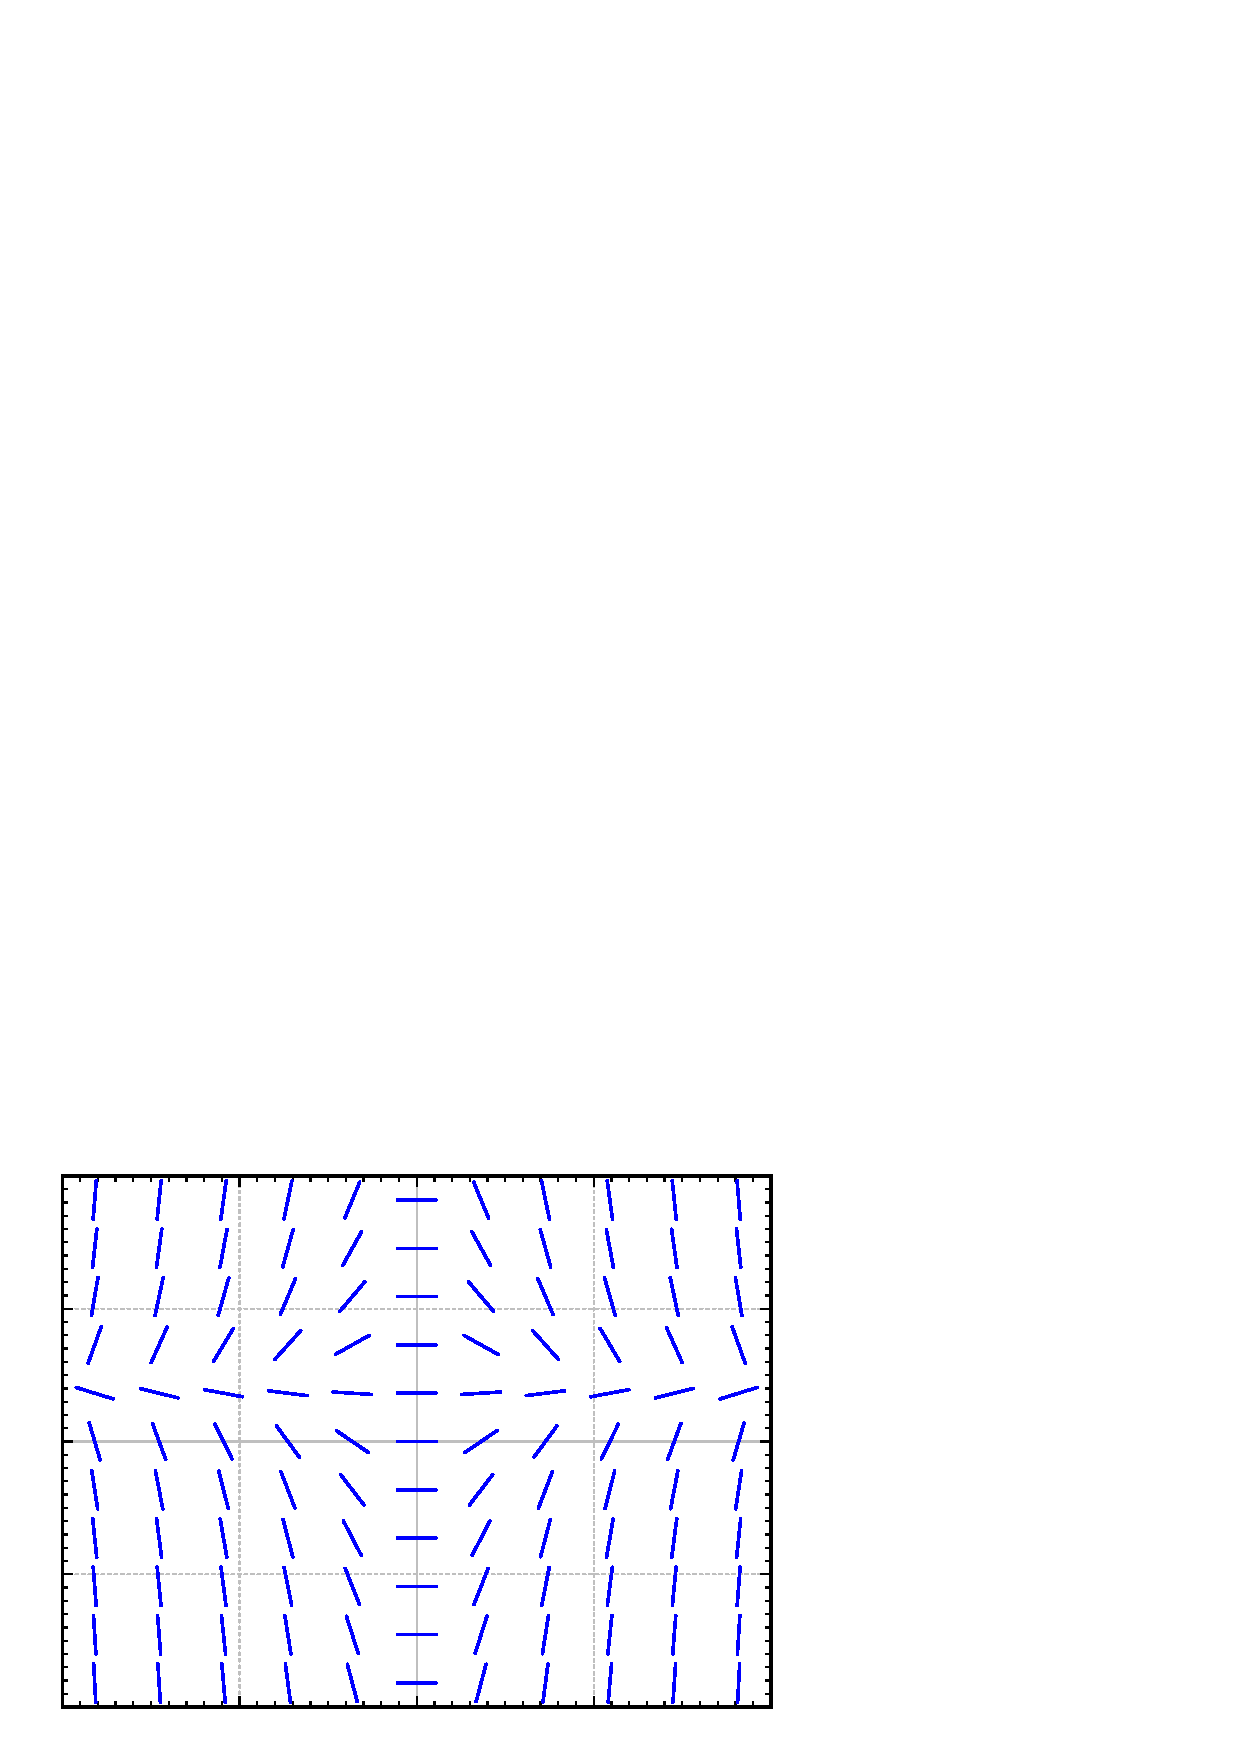
\includegraphics[width=1.75in]{figures/yprimex1minusyslope}}
\task
\parbox[c]{1.75in}{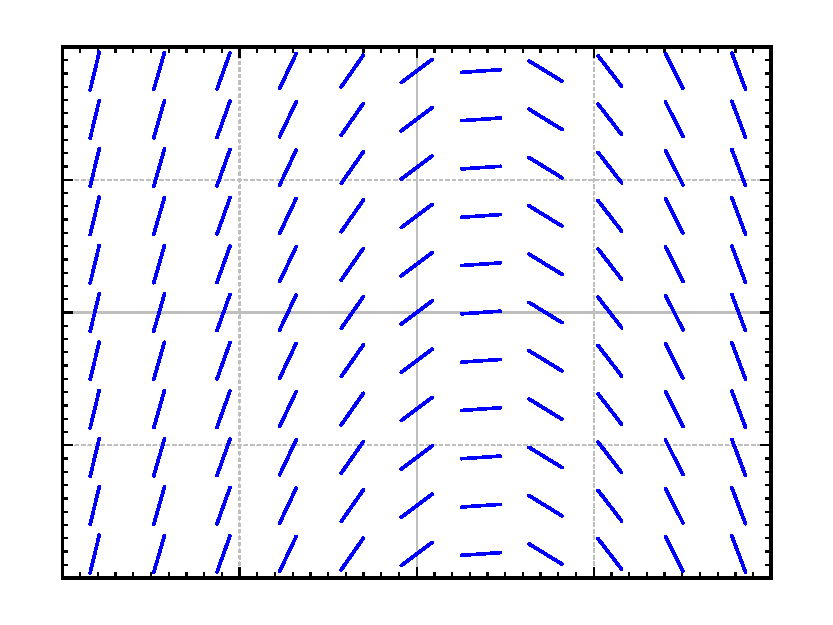
\includegraphics[width=1.75in]{figures/yprime1minusxslope}}
\task
\parbox[c]{1.75in}{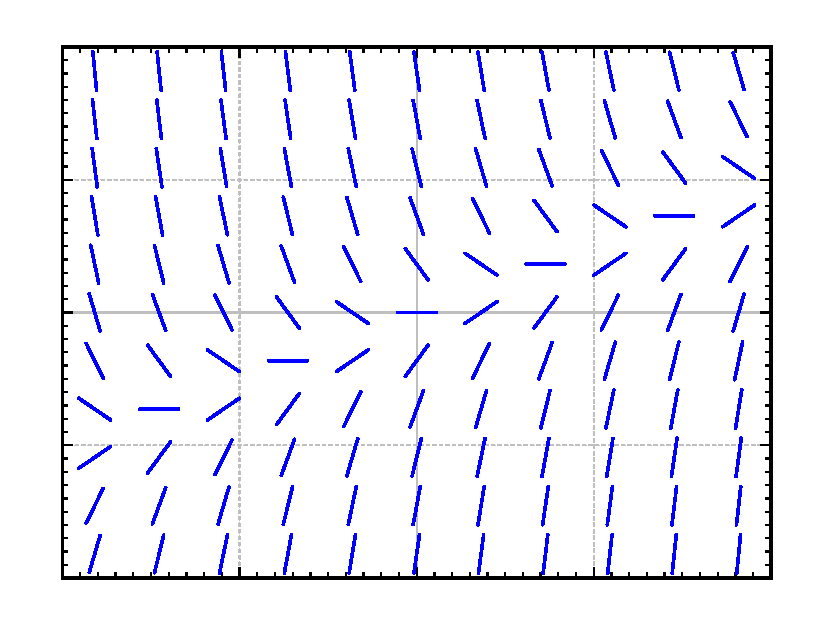
\includegraphics[width=1.75in]{figures/yprimexminus2yslope}}
\end{tasks}
\end{exercise}
\end{samepage}

\begin{exercise}[challenging]
Take $y' = f(x,y)$, $y(0) = 0$, where $f(x,y) > 1$
for all $x$ and $y$.  If
the solution exists for all $x$, can you say
what happens to $y(x)$ as $x$ goes to positive infinity?  Explain.
\end{exercise}

\begin{exercise}[challenging]
Take $(y-x)y' = 0$, $y(0) = 0$.
\begin{tasks}
\task Find two distinct solutions.
\task Explain why this does not violate Picard's theorem.  
\end{tasks}
\end{exercise}

\begin{exercise}
Suppose $y' = f(x,y)$.  What will the slope field look like, explain and
sketch an example, if you know the following about $f(x,y)$:
\begin{tasks}(2)
\task $f$ does
not depend on $y$.
\task $f$ does not depend on $x$.
\task $f(t,t) = 0$ for any
number $t$.
\task $f(x,0) = 0$ and $f(x,1) = 1$ for all $x$.
\end{tasks}
\end{exercise}

\begin{exercise}
Find a solution to $y' = \lvert y \rvert$, $y(0) = 0$.  Does Picard's theorem apply?
\end{exercise}

\begin{exercise}
Take an equation $y' = (y-2x) g(x,y) + 2$ for some function $g(x,y)$.
Can you solve the problem for the
initial condition $y(0) = 0$,
and if so what is the solution?
\end{exercise}

\begin{exercise}[challenging]
\pagebreak[2]
Suppose $y' = f(x,y)$ is such that $f(x,1) = 0$ for every $x$,
$f$ is continuous and $\frac{\partial f}{\partial y}$ exists and
is continuous for every $x$ and $y$.
\begin{tasks}
\task
Guess a solution given the initial condition
$y(0) = 1$.
\task
Can graphs of two solutions of the equation for different initial conditions
ever intersect?
\task
Given $y(0) = 0$, what can you say about the solution.  In particular,
can $y(x) > 1$ for any $x$?  Can $y(x) = 1$ for any $x$?  Why or why not?
\end{tasks}
\end{exercise}

\setcounter{exercise}{100}

\begin{exercise}
Sketch the slope field of $y'=y^3$.  Can you visually find the solution
that satisfies $y(0)=0$?
\end{exercise}
\exsol{%
%mbxSTARTIGNORE
\vtop{\vskip-1ex \hbox{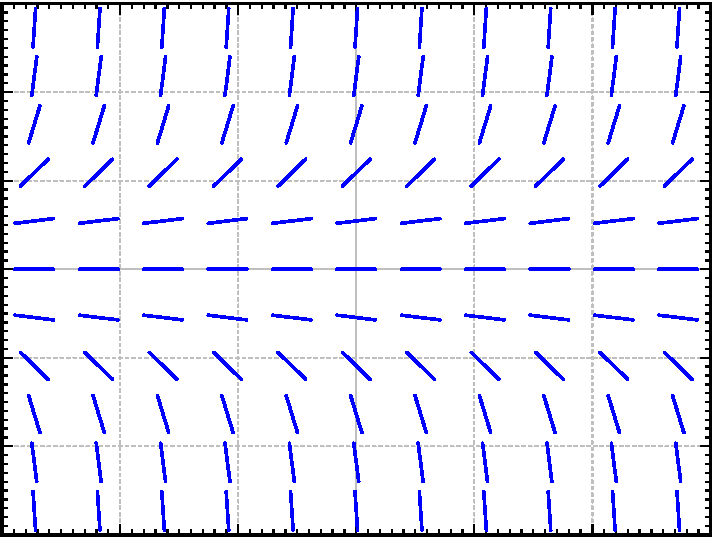
\includegraphics[width=2in]{figures/yprimey3slope}}}
\quad
%mbxENDIGNORE
%mbxlatex \\
%mbxlatex 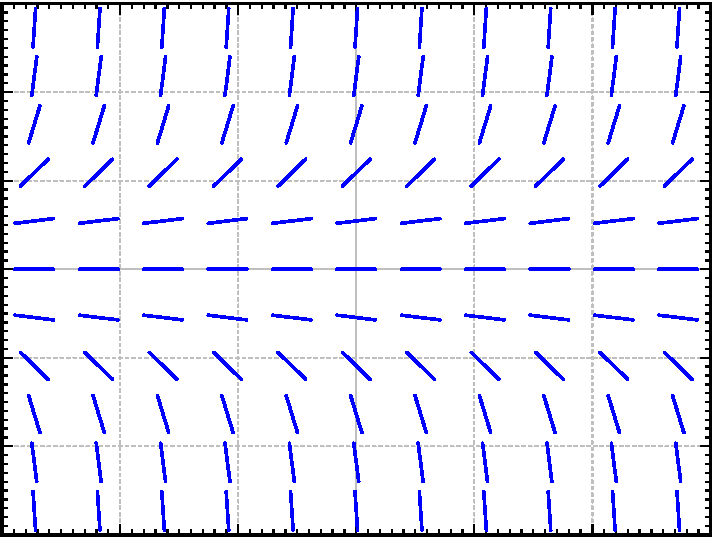
\includegraphics[width=2in]{figures/yprimey3slope}
%mbxlatex \\
$y=0$ is a solution such that $y(0)=0$.
}

\begin{exercise}
Is it possible to solve $y' = xy$ for $y(0) = 0$?  Is the solution unique?
\end{exercise}
\exsol{%
Yes a solution exists.  The equation is $y' = f(x,y)$ where $f(x,y) = xy$.  The function
$f(x,y)$ is continuous and 
$\frac{\partial f}{\partial y} = x$, which is also continuous near $(0,0)$.
So a solution exists and is unique.  (In fact, $y=0$ is the solution.)
}

\begin{exercise}
Is it possible to solve $y' = \frac{x}{x^2-1}$ for $y(1) = 0$?
\end{exercise}
\exsol{%
No, the equation is not defined at $(x,y) = (1,0)$.
}

\begin{samepage}
\begin{exercise}
Match equations $y'=\sin x$, $y'=\cos y$, $y' = y\cos(x)$ to slope fields.
Justify.
\begin{tasks}(3)
\task
\parbox[c]{1.75in}{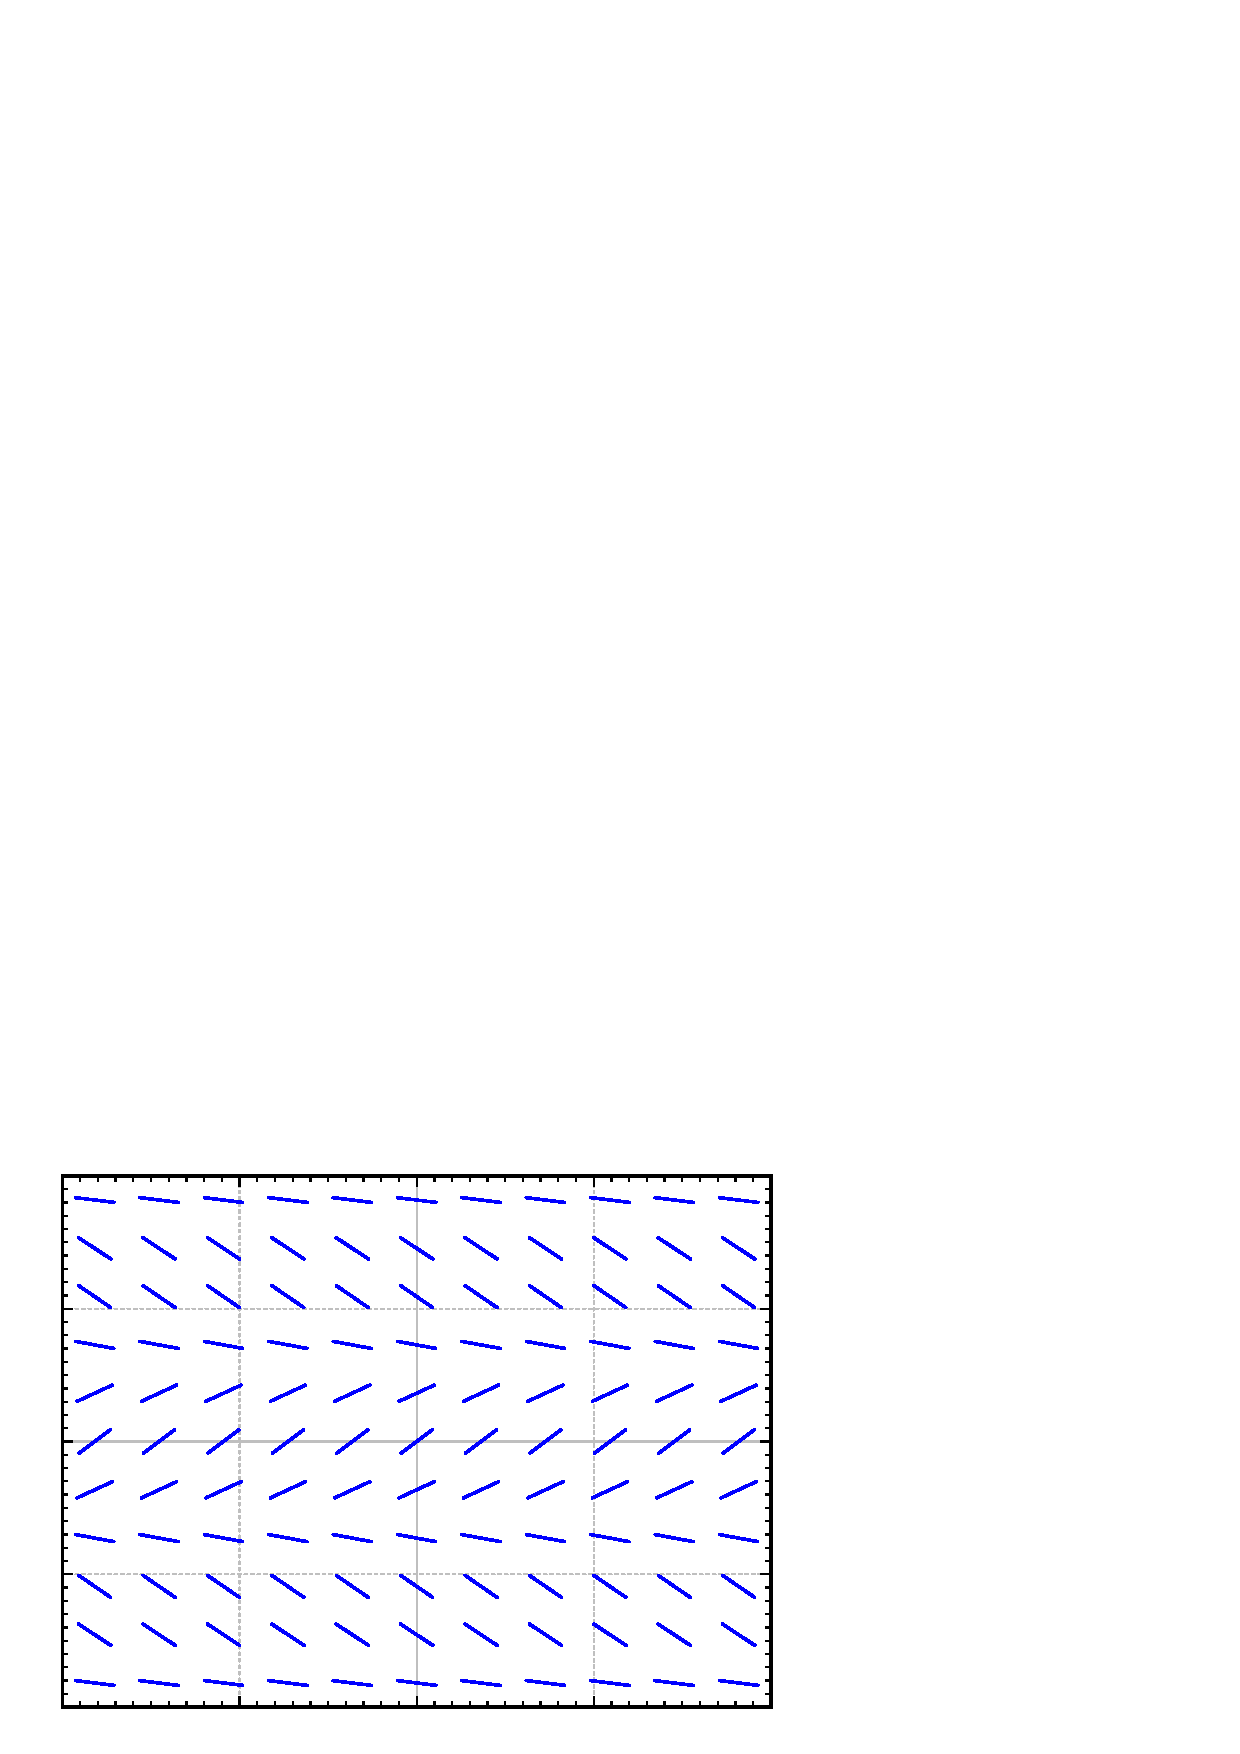
\includegraphics[width=1.75in]{figures/yprimecosyslope}}
\task
\parbox[c]{1.75in}{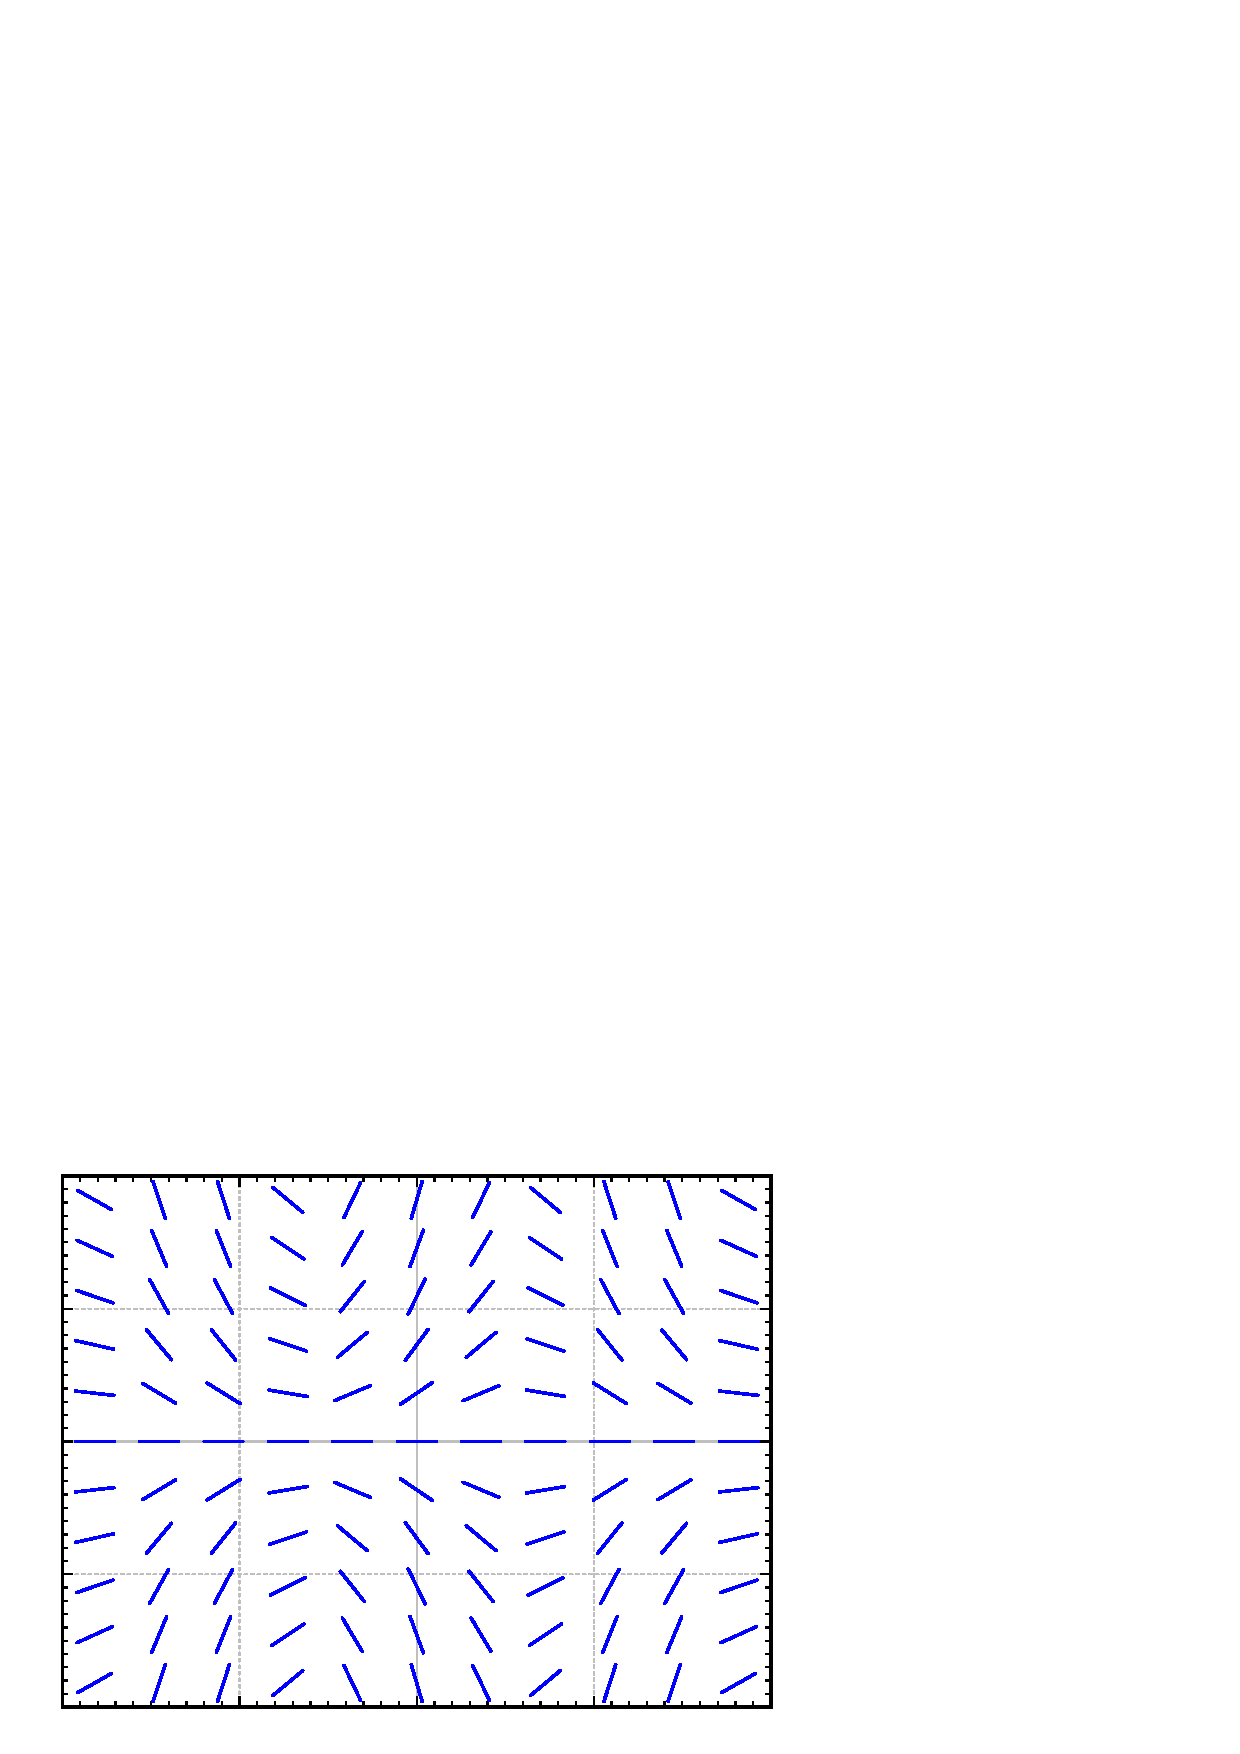
\includegraphics[width=1.75in]{figures/yprimecosxyslope}}
\task
\parbox[c]{1.75in}{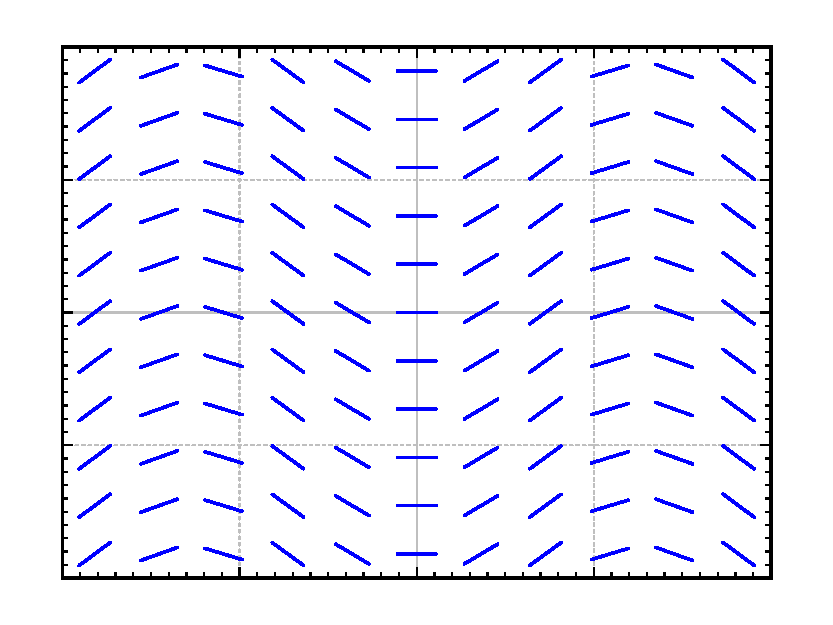
\includegraphics[width=1.75in]{figures/yprimesinxslope}}
\end{tasks}
\end{exercise}
\end{samepage}
\exsol{%
a) $y'=\cos y$, \quad
b) $y' = y\cos(x)$, \quad
c) $y'=\sin x$. \quad
Justification left to reader.
}

\begin{exercise}[tricky]
Suppose
\begin{equation*}
f(y) =
\begin{cases}
0 & \text{ if $y > 0$}, \\
1 & \text{ if $y \leq 0$} .
\end{cases}
\end{equation*}
Does $y' = f(y)$, $y(0) = 0$ have a continuously differentiable solution?  Does Picard apply?  Why, or why not?
\end{exercise}
\exsol{%
Picard does not apply as $f$ is not continuous at $y=0$.
The equation does not have a continuously differentiable solution.
Suppose it did. Notice that
$y'(0) = 1$.  By the first derivative test, $y(x) > 0$ for small positive $x$.
But then for those $x$ we would have $y'(x) = 0$, so clearly the derivative
cannot be continuous.
}

\begin{exercise}
Consider an equation of the form $y' = f(x)$ for some continuous function
$f$, and an initial condition $y(x_0) = y_0$.  Does a
solution exist for all $x$?  Why or why not?
\end{exercise}
\exsol{%
The solution is $y(x) = \int_{x_0}^x f(s) \,ds + y_0$, and this does indeed
exist for every $x$.
}

%%%%%%%%%%%%%%%%%%%%%%%%%%%%%%%%%%%%%%%%%%%%%%%%%%%%%%%%%%%%%%%%%%%%%%%%%%%%%%

\sectionnewpage
\section{Separable equations}
\label{separable:section}

\sectionnotes{1 lecture\EPref{, \S1.4 in \cite{EP}}\BDref{,
\S2.2 in \cite{BD}}}

When a differential equation is of the form
$y' = f(x)$,
we can just integrate:
$y = \int f(x) \,dx + C$. 
Unfortunately this method no longer works for the
general form of the equation
$y' = f(x,y)$.
Integrating both sides yields
\begin{equation*}
y = \int f(x,y) \,dx + C .
\end{equation*}
Notice the dependence on $y$ in the integral.

\subsection{Separable equations}

We say a differential equation is
\emph{\myindex{separable}}
if we can write it as
\begin{equation*}
y' = f(x)g(y) ,
\end{equation*}
for some functions $f(x)$ and $g(y)$.
Let us write the equation in the \myindex{Leibniz notation}
\begin{equation*}
\frac{dy}{dx} = f(x)g(y) .
\end{equation*}
Then we rewrite the equation as
\begin{equation*}
\frac{dy}{g(y)} = f(x) \,dx .
\end{equation*}
Both sides look like something we can integrate.  We obtain
\begin{equation*}
\int \frac{dy}{g(y)} = \int f(x) \,dx + C .
\end{equation*}
If we can find closed form expressions
for these two integrals, we can, perhaps, solve for $y$.

\begin{example} \label{example:yprimeisxy}
Take the equation
\begin{equation*}
y' = xy .
\end{equation*}
Note that $y=0$ is a solution.  We will remember that fact and
assume $y \not =0$ from now on, so that we can divide by $y$.
Write the equation as $\frac{dy}{dx} = xy$. Then
\begin{equation*}
\int \frac{dy}{y} = \int x\,dx + C .
\end{equation*}
We compute the antiderivatives to get
\begin{equation*}
\ln \, \lvert y\rvert = \frac{x^2}{2} + C ,
\end{equation*}
or
\begin{equation*}
\lvert y \rvert = e^{\frac{x^2}{2} + C} = e^{\frac{x^2}{2}} e^C = D e^{\frac{x^2}{2}} ,
\end{equation*}
where $D > 0$ is some constant.  Because $y=0$ is also a solution and because
of the absolute value we can write:
\begin{equation*}
y = D e^{\frac{x^2}{2}} ,
\end{equation*}
for any number $D$ (including zero or negative).

We check:
\begin{equation*}
y' = D x e^{\frac{x^2}{2}} = x \left( D e^{\frac{x^2}{2}} \right) = xy .
\end{equation*}
Yay!
\end{example}

We should be a little bit more careful with this method.  You may be worried 
that we 
integrated in two different variables.
We seemingly did
a different operation to each side.  Let us work through this method more
rigorously.  Take
\begin{equation*}
\frac{dy}{dx} = f(x)g(y) .
\end{equation*}
We rewrite the equation as follows.
Note that $y = y(x)$ is a function of $x$ and so is
$\frac{dy}{dx}$!
\begin{equation*}
\frac{1}{g(y)}\,\frac{dy}{dx} = f(x) .
\end{equation*}
We integrate both sides with respect to $x$:
\begin{equation*}
\int \frac{1}{g(y)}\,\frac{dy}{dx} \,dx = \int f(x) \,dx + C .
\end{equation*}
We use the change of variables formula (substitution) on the left hand side:
\begin{equation*}
\int \frac{1}{g(y)}\,dy = \int f(x) \,dx + C .
\end{equation*}
And we are done.

\subsection{Implicit solutions}

We sometimes get stuck even if we can do the
integration.  Consider the separable equation
\begin{equation*}
y' = \frac{xy}{y^2+1} .
\end{equation*}
We separate variables,
\begin{equation*}
\frac{y^2+1}{y}\,dy = \left(y+\frac{1}{y}\right)\,dy = x\,dx .
\end{equation*}
We integrate to get
\begin{equation*}
\frac{y^2}{2} + \ln \, \lvert y \rvert = \frac{x^2}{2} + C ,
\end{equation*}
or perhaps the easier looking expression (where $D = 2C$)
\begin{equation*}
y^2 + 2 \ln \, \lvert y\rvert = x^2 + D .
\end{equation*}
It is not easy to find the solution explicitly as it is hard to solve
for $y$.  We, therefore, leave the solution in this form and call
it an
\emph{\myindex{implicit solution}}.
It is still
easy to check that an implicit solution satisfies the differential
equation.  In this case, we differentiate with respect to $x$, and remember
that $y$ is a function of $x$,
to get
\begin{equation*}
y'\left(2y + \frac{2}{y}\right) = 2x .
\end{equation*}
Multiply both sides by $y$ and divide by $2(y^2+1)$ and you will
get exactly the differential equation.  We leave this computation to the
reader.

If you have an implicit solution, and
you want to compute values
for $y$, you might have to be tricky.  You might get multiple solutions $y$
for each $x$, so you have to pick one.  Sometimes you can
graph $x$ as a function of $y$, and then flip your paper.
Sometimes you have to do more.

Computers are also good at some of these tricks.
More advanced mathematical software usually has some
way of plotting solutions to implicit equations.
For example, for $C=0$ if you plot all the points $(x,y)$ that
are solutions to $y^2+2\ln|y|=x^2$,
you find the two curves in \figurevref{implicitsols:fig}.  This is not quite
a graph of a function. For each $x$ there are two choices of $y$.
To find a function you would have to pick one of these two curves.
You pick the one that satisfies your initial condition if you have one.
For example, the top curve satisfies the condition $y(1)=1$.
So for each $C$ we really got two solutions.
As you can see, computing values from an implicit solution can be somewhat
tricky.  But sometimes, an implicit solution is the best we can do.

\begin{myfig}
\capstart
\diffyincludegraphics{width=3in}{width=4.5in}{implicitsols}
\caption{The implicit solution $y^2+2\ln|y|=x^2$ to $y'=\frac{xy}{y^2+1}$.\label{implicitsols:fig}}
\end{myfig}


The equation above also has the solution $y=0$.
So the general solution is 
\begin{equation*}
y^2 + 2 \ln \, \lvert y \rvert = x^2 + C, \qquad \text{and} \qquad y=0.
\end{equation*}
These outlying solutions
such as $y=0$
are sometimes called \emph{singular solutions\index{singular solution}}.

\subsection{Examples of separable equations}

\begin{example}
Solve $x^2y' = 1 - x^2+y^2 - x^2y^2$, $y(1) = 0$.

Factor the right-hand side
\begin{equation*}
x^2y' = (1 - x^2)(1+y^2) .
\end{equation*}
Separate variables, integrate, and solve for $y$:
\begin{align*}
\frac{y'}{1+y^2} & = \frac{1 - x^2}{x^2} , \\
\frac{y'}{1+y^2} & = \frac{1}{x^2} - 1 , \\
\operatorname{arctan} (y) & = \frac{-1}{x} - x + C , \\
y & = \tan \left(\frac{-1}{x} - x + C\right) .
\end{align*}
Solve for the initial condition, $0 = \tan(-2+C)$ to get $C=2$ (or $C = 2 +
\pi$, or $C = 2 + 2\pi$, etc.).  The particular solution we seek is, therefore,
\begin{equation*}
y = \tan \left(\frac{-1}{x} - x + 2 \right) .
\end{equation*}
\end{example}

\begin{example} \label{sep:coffeeexample}
Bob made a cup of coffee, and
Bob likes to drink coffee only once reaches 60 degrees Celsius and will not burn him.
Initially at time $t=0$ minutes,
Bob measured the temperature and the coffee was 89 degrees Celsius.
One minute later, Bob measured the coffee again and it had 85 degrees.
The temperature of the room (the ambient temperature) is 22 degrees.
When should Bob start drinking?

Let $T$ be the temperature of the coffee in degrees Celsius, and let $A$ be
the ambient (room) temperature, also in degrees Celsius.
\myindex{Newton's law of cooling} states that the rate at which the
temperature of the coffee is changing
is proportional to the difference between the
ambient temperature and the temperature of the coffee.  That is,
\begin{equation*}
\frac{dT}{dt} = k(A-T) ,
\end{equation*}
for some positive constant $k$.
For our setup $A=22$, $T(0) = 89$, $T(1) = 85$.
We separate variables and integrate (let $C$ and $D$ denote arbitrary
constants):
\begin{align*}
\frac{1}{T-A} \, \frac{dT}{dt} & = -k , \\
\ln (T-A) &= -kt + C , \qquad \text{(note that } T-A > 0 \text{)} \\
T-A &= D\, e^{-kt} ,  \\
T &= A + D\, e^{-kt} .
\end{align*}
That is,
$T = 22 + D\, e^{-kt}$.  We plug in the first condition: $89 = T(0) = 22 +
D$,
and hence $D = 67$.  So
$T = 22 + 67\, e^{-kt}$.  The second condition says $85 = T(1) = 
22 + 67\, e^{-k}$.  Solving for $k$ we get
$k = - \ln \frac{85-22}{67} \approx 0.0616$.  Now we solve for the time $t$
that gives us a temperature of 60 degrees.  Namely, we solve
\begin{equation*}
60 = 22 + 67 e^{-0.0616t}
\end{equation*}
to get
$t = - \frac{\ln \frac{60-22}{67}}{0.0616} \approx 9.21$ minutes.  So Bob can
begin to drink the coffee at just over 9 minutes from the time Bob made
it.  That is probably about the amount of time it took us to calculate how long
it would take.  See \figurevref{sintro:coffeefig}.
\begin{myfig}
\capstart
%original files coffeefig-1 coffeefig-2
\diffyincludegraphics{width=6.24in}{width=9in}{coffeefig-1-2}
\caption{Graphs of the coffee temperature function $T(t)$.
On the left, horizontal
lines are drawn at temperatures 60, 85, and 89.  Vertical lines
are drawn at $t=1$ and $t=9.21$.  Notice that the
temperature of the coffee hits 85 at $t=1$, and 60 at
$t \approx 9.21$.  On the right, the graph is over a longer period of time,
with a horizontal line at the ambient temperature 22.\label{sintro:coffeefig}}
\end{myfig}
\end{example}

\begin{example}
Find the general solution to $y' = \frac{-xy^2}{3}$ (including singular
solutions).

First note that $y=0$ is a solution (a singular solution).
Now assume that $y \not= 0$.
\begin{align*}
\frac{-3}{y^2} y' & = x , \displaybreak[0]\\
\frac{3}{y} & = \frac{x^2}{2} + C , \displaybreak[0]\\
y & = \frac{3}{\nicefrac{x^2}{2} + C}
= \frac{6}{x^2 + 2C}.
\end{align*}
So the general solution is
\begin{equation*}
y = \frac{6}{x^2 + 2C} \qquad \text{and} \qquad y=0 .
\end{equation*}
\end{example}

\subsection{Exercises}

\begin{exercise}
Solve $y' = \nicefrac{x}{y}$.
\end{exercise}

\begin{exercise}
Solve $y' = x^2y$.
\end{exercise}

\begin{exercise}
Solve $\dfrac{dx}{dt} = (x^2-1)\,t$, for $x(0) = 0$.
\end{exercise}

\begin{exercise}
Solve $\dfrac{dx}{dt} = x\,\sin(t)$, for $x(0) = 1$.
\end{exercise}

\begin{exercise}
Solve $\dfrac{dy}{dx} = xy+x+y+1$.  Hint: Factor the right-hand side.
\end{exercise}

\begin{exercise}
Solve $xy' = y + 2x^2 y$, where $y(1) = 1$.
\end{exercise}

\begin{exercise}
Solve $\dfrac{dy}{dx} = \dfrac{y^2+1}{x^2+1}$, for $y(0) = 1$.
\end{exercise}

\begin{exercise}
Find an implicit solution for
$\dfrac{dy}{dx} = \dfrac{x^2+1}{y^2+1}$, for $y(0) = 1$.
\end{exercise}

\begin{exercise}
Find an explicit solution for $y' = xe^{-y}$, $y(0)=1$.
\end{exercise}

\begin{exercise}
Find an explicit solution for $xy' = e^{-y}$, for $y(1)=1$.
\end{exercise}

\begin{exercise}
Find an explicit solution for $y' = ye^{-x^2}$, $y(0)=1$.  It is alright to
leave a definite integral in your answer.
\end{exercise}

\begin{exercise}
Suppose a cup of coffee is at 100 degrees Celsius at time $t=0$,
it is at 70 degrees at $t=10$ minutes, and it is at 50 degrees at $t=20$
minutes.  Compute the ambient temperature.
\end{exercise}

\setcounter{exercise}{100}

\begin{exercise}
Solve $y'=2xy$.
\end{exercise}
\exsol{%
$y = Ce^{x^2}$
}

\begin{exercise}
Solve $x'=3xt^2-3t^2$, $x(0)=2$.
\end{exercise}
\exsol{%
$x = e^{t^3}+1$
}

\begin{exercise}
Find an implicit solution for
$x'=\frac{1}{3x^2+1}$, $x(0)=1$.
\end{exercise}
\exsol{%
$x^3+x=t+2$
}

\begin{exercise}
Find an explicit solution to $x y' = y^2$, $y(1) = 1$.
\end{exercise}
\exsol{%
$y = \frac{1}{1-\ln x}$
}

\begin{exercise}
Find an implicit solution to $y' = \frac{\sin(x)}{\cos(y)}$.
\end{exercise}
\exsol{%
$\sin(y) = -\cos(x) + C$
}

\begin{exercise}
Take \exampleref{sep:coffeeexample} with the same numbers: 89 degrees at
$t=0$, 85 degrees at $t=1$, and ambient temperature
of 22 degrees.  Suppose these temperatures were measured with precision of
$\pm 0.5$ degrees.  Given this imprecision, the time
it takes the coffee to cool to (exactly) 60 degrees is also only known in a
certain range.  Find this range.  Hint: Think about what kind of error makes
the cooling time longer and what shorter.
\end{exercise}
\exsol{%
The range is approximately 7.45 to 12.15 minutes.
}

\begin{exercise}
A population $x$ of rabbits on an island is modeled by
$x' = x- \bigl(\nicefrac{1}{1000} \bigr) x^2$, where the independent
variable is time in months.  At time $t=0$, there are 40 rabbits
on the island.
\begin{tasks}
\task Find the solution to the equation with the initial
condition.
\task
How many rabbits are on the island in 1 month, 5 months, 
10 months, 15 months (round to the nearest integer).
\end{tasks}
\end{exercise}
\exsol{%
a) $x = \frac{1000e^t}{e^t+24}$. \quad b) 102 rabbits after one month,
861 after 5 months, 999 after 10 months, 1000 after 15 months.
}

%%%%%%%%%%%%%%%%%%%%%%%%%%%%%%%%%%%%%%%%%%%%%%%%%%%%%%%%%%%%%%%%%%%%%%%%%%%%%%

\sectionnewpage
\section{Linear equations and the integrating factor}
\label{intfactor:section}

\sectionnotes{1 lecture\EPref{, \S1.5 in \cite{EP}}\BDref{,
\S2.1 in \cite{BD}}}

One of the most important types of equations we will learn how to solve are
the so-called
\emph{linear equations\index{linear equation}}.
In fact, the majority of the course is about linear
equations.  In this section we focus on the
\emph{\myindex{first order linear equation}}.
A first order equation is linear if we can put it
into the form:
\begin{equation} \label{lineq:eq1}
y' + p(x) y = f(x) .
\end{equation}
The word
\myquote{linear} means linear in $y$ and $y'$;
no higher powers nor functions of $y$ or $y'$ appear.
The dependence on $x$ can be more
complicated.

Solutions of linear equations have nice properties.  For example, the
solution exists wherever $p(x)$ and $f(x)$ are defined, and has the same
regularity (read: it is just as nice).  But most importantly for us right now,
there is a method for solving linear first order equations.

The trick is to rewrite the left-hand side
of \eqref{lineq:eq1} as a derivative of a product of $y$ with another
function.
To this end
we find a function $r(x)$ such that
\begin{equation*}
r(x) y' + r(x) p(x) y = \frac{d}{dx}\Bigl[ r(x) y \Bigr] .
\end{equation*}
This is the left-hand side of
\eqref{lineq:eq1} multiplied by $r(x)$.  So if we multiply \eqref{lineq:eq1} by
$r(x)$, we obtain
\begin{equation*}
\frac{d}{dx}\Bigl[ r(x) y \Bigr] = r(x)f(x) .
\end{equation*}
Now we integrate both sides.
The right-hand side does not depend on $y$ and the left-hand side
is written as a derivative of a function.  Afterwards, we solve for $y$.
The function $r(x)$ is called the \emph{\myindex{integrating factor}} and the
method is called the \emph{\myindex{integrating factor method}}.

We are looking for a function $r(x)$, such that if
we differentiate it, we get the same function back multiplied by $p(x)$.
That seems like a job for the exponential function!  Let
\begin{equation*}
r(x) = e^{\int p(x) \,dx} .
\end{equation*}
We compute:
\begin{align*}
y' + p(x) y &= f(x) , \\
e^{\int p(x) \,dx} y' + e^{\int p(x) \,dx} p(x) y & = e^{\int p(x) \,dx} f(x) , \\
\frac{d}{dx}\left[ e^{\int p(x) \,dx} y \right] & = e^{\int p(x) \,dx} f(x) , \\
e^{\int p(x) \,dx} y & = \int e^{\int p(x) \,dx} f(x) \,dx + C , \\
y & = e^{-\int p(x) \,dx} \left( \int e^{\int p(x) \,dx} f(x) \,dx + C \right) .
\end{align*}

Of course, to get a closed form formula for $y$,
we need to be able to find a
closed form formula for the integrals appearing above.

\begin{example}
Solve
\begin{equation*}
y' + 2xy = e^{x-x^2}, \qquad y(0) = -1 .
\end{equation*}

First note that $p(x) = 2x$ and $f(x) = e^{x-x^2}$.
The integrating factor is $r(x) = e^{\int p(x)\, dx} = e^{x^2}$.
We multiply both sides of the equation by $r(x)$ to get
\begin{align*}
e^{x^2} y' + 2xe^{x^2}y & = e^{x-x^2} e^{x^2} , \\
\frac{d}{dx} \left[ e^{x^2} y \right] &= e^x .
\end{align*}
We integrate
\begin{align*}
e^{x^2} y &= e^x +C , \\
y &= e^{x-x^2} + C e^{-x^2} .
\end{align*}
Next, we solve for the initial condition $-1 = y(0) = 1 + C$, so $C=-2$.
The solution is
\begin{equation*}
y = e^{x-x^2} - 2 e^{-x^2} .
\end{equation*}
\end{example}

Note that we do not care which antiderivative we take when computing
$e^{\int p(x) dx}$.  You can always add a constant of integration,
but those constants
will not matter in the end.

\begin{exercise}
Try it!  Add a constant of integration to the integral in
the integrating factor and show that the solution you get in the end is the
same as what we got above.
\end{exercise}

Advice: Do not try to remember the formula itself, that is way too
hard.  It is easier to remember the process and repeat it.

Since we cannot always evaluate the integrals in closed form, it is useful to
know how to write the solution in definite integral form.  A definite
integral is something that
you can plug into a computer or a calculator.  Suppose we are given
\begin{equation*}
y' + p(x) y = f(x) , \qquad y(x_0) = y_0 .
\end{equation*}
Look at the solution and write the integrals
as definite integrals.
\begin{equation} \label{lei:defsol}
\mybxbg{
~~
y(x) = e^{-\int_{x_0}^x p(s)\, ds} \left( \int_{x_0}^x e^{\int_{x_0}^t p(s)\, ds}
f(t) \,dt + y_0 \right).
~~
}
\end{equation}
You should
be careful to properly use dummy variables here.  If you now plug such a
formula into a
computer or a calculator, it will be happy to give you numerical answers.

\begin{exercise}
Check that $y(x_0) = y_0$ in formula \eqref{lei:defsol}.
\end{exercise}

\begin{exercise}
Write the solution of the following problem
as a definite integral, but try to simplify as far as you can.  You will not
be able to find the solution in closed form.
\begin{equation*}
y' + y = e^{x^2-x}, \qquad y(0) = 10 .
\end{equation*}
\end{exercise}

\begin{remark}
Before we move on, we should note some interesting properties of linear
equations.  First, for the linear initial value problem
$y' + p(x) y = f(x)$, $y(x_0) = y_0$,
there is always an explicit formula \eqref{lei:defsol} for the
solution.  Second, it follows
from the formula \eqref{lei:defsol} that if $p(x)$
and $f(x)$ are continuous on some interval $(a,b)$, then the 
solution $y(x)$ exists and is differentiable on $(a,b)$.  Compare
with the simple nonlinear example we have seen previously, $y'=y^2$,
and compare to \thmref{slope:picardthm}.
\end{remark}


\begin{example}
Let us discuss a common
simple application of linear equations.
This type of 
problem is used often in real life.
For example, linear equations are used in
figuring out the concentration of
chemicals in bodies of water (rivers and lakes).

\begin{mywrapfigsimp}{1.60in}{1.65in}
\noindent
\inputpdft{lin-tank}
\end{mywrapfigsimp}
A 100 liter tank contains 10 kilograms of salt dissolved in 60 liters of
water.  Solution of water and salt (brine) with concentration of 0.1
kilograms per
liter is flowing in at the rate of 5 liters a minute.  The solution
in the tank is well stirred and flows out at a rate of 3 liters a minute.
How much salt is in the tank when the tank is full?

Let us come up with the equation.  Let $x$ denote the kilograms of salt in the tank,
let $t$ denote the time in minutes.  For a small change $\Delta t$ in
time, the change in $x$ (denoted $\Delta x$) is approximately
\begin{equation*}
\Delta x \approx
(\text{rate in} \times \text{concentration in}) \Delta t - 
(\text{rate out} \times \text{concentration out}) \Delta t .
\end{equation*}
Dividing through by $\Delta t$ and
taking the limit $\Delta t \to 0$, we see that
\begin{equation*}
\frac{dx}{dt} =
(\text{rate in} \times \text{concentration in})  - 
(\text{rate out} \times \text{concentration out}) .
\end{equation*}
In our example,
\begin{align*}
\text{rate in} &= 5 , \\
\text{concentration in} &= 0.1 , \\
\text{rate out} &= 3 , \\
\text{concentration out} &= \frac{x}{\text{volume}} = \frac{x}{60+(5-3)t} .
\end{align*}
Our equation is, therefore,
\begin{equation*}
\frac{dx}{dt} =
(5 \times 0.1)  - 
\left(3 \frac{x}{60+2t}\right) .
\end{equation*}
Or in the form \eqref{lineq:eq1}
\begin{equation*}
\frac{dx}{dt} +
\frac{3}{60+2t} x
=
0.5 .
\end{equation*}

Let us solve.  The integrating factor is
\begin{equation*}
r(t) = \exp \left( \int \frac{3}{60+2t} dt  \right)
=
\exp \left( \frac{3}{2} \ln (60+2t) \right)
=
{(60+2t)}^{3/2} .
\end{equation*}
We multiply both sides of the equation to get
\begin{align*}
{(60+2t)}^{3/2} \frac{dx}{dt} +
{(60+2t)}^{3/2} \frac{3}{60+2t} x
& =
0.5{(60+2t)}^{3/2} ,\\
\frac{d}{dt}\left[
{(60+2t)}^{3/2} x \right]
& =
0.5{(60+2t)}^{3/2} ,\\
{(60+2t)}^{3/2} x
& =
\int 
0.5{(60+2t)}^{3/2}
dt
+C ,\\
 x
& =
{(60+2t)}^{-3/2} \int 
\frac{
{(60+2t)}^{3/2}
}{2}
dt
+C{(60+2t)}^{-3/2} ,\\
 x
& =
{(60+2t)}^{-3/2}
\frac{1}{10}{(60+2t)}^{5/2}
+C{(60+2t)}^{-3/2} ,\\
 x
& =
\frac{60+2t}{10}
+C{(60+2t)}^{-3/2} .
\end{align*}

%mbxSTARTIGNORE
\begin{mywrapfig}{3.25in}
\capstart
\diffyincludegraphics{width=3in}{width=4.5in}{linear-salt-graph}
\caption{Graph of the solution $x$ kilograms of salt in the tank at time
$t$.\label{linear-salt-graph:fig}}
\end{mywrapfig}
%mbxENDIGNORE
%
% Make sure to keep the above and the mbx figure below in sync!
%
To find $C$, note that at $t=0$, we have $x=10$.  That is,
\begin{equation*}
10 = x(0)
=
\frac{60}{10}
+C{(60)}^{-3/2}
=
6
+C{(60)}^{-3/2} ,
\end{equation*}
or
\begin{equation*}
C=4 ({60}^{3/2}) \approx 1859.03 .
\end{equation*}

We know $5$ liters per minute are flowing in and $3$ liters per minute are flowing out,
so the volume is increasing by $2$ liters a minute.
So the tank is
full when $60+2t = 100$, or when $t=20$.
We are interested in the value of $x$ when the tank is full,
that is we want to compute $x(20)$:
\begin{equation*}
\begin{split}
x(20) & = 
\frac{60+40}{10}
+C{(60+40)}^{-3/2}
\\
& \approx
10
+1859.03 {(100)}^{-3/2}
\approx
11.86 .
\end{split}
\end{equation*}
See \figurevref{linear-salt-graph:fig} for the graph of $x$ over $t$.

The concentration when the tank is full is approximately
$\nicefrac{11.86}{100} = \unitfrac[0.1186]{kg}{liter}$, and we started
with $\nicefrac{1}{6}$ or \unitfrac[0.167]{kg}{liter}.
%mbxlatex \begin{myfig}
%mbxlatex \capstart
%mbxlatex \diffyincludegraphics{width=3in}{width=4.5in}{linear-salt-graph}
%mbxlatex \caption{Graph of the solution $x$ kilograms of salt in the tank at time
%mbxlatex $t$.\label{linear-salt-graph:fig}}
%mbxlatex \end{myfig}
\end{example}

\subsection{Exercises}

In the exercises, feel free to leave answer as a definite integral if a
closed form solution cannot be found.  If you can find a closed form
solution, you should give that.

\begin{exercise}
Solve $y' + xy = x$.
\end{exercise}

\begin{exercise}
Solve $y' + 6y = e^x$.
\end{exercise}

\begin{exercise}
Solve $y' + 3x^2y = \sin(x) \, e^{-x^3}$, with $y(0) = 1$.
\end{exercise}

\begin{exercise}
Solve $y' + \cos (x) y = \cos(x)$.
\end{exercise}

\begin{exercise}
Solve $\frac{1}{x^2+1} \, y' + x y = 3$, with $y(0) = 0$.
\end{exercise}

\begin{exercise}
Suppose there are two lakes located on a stream.  Clean
water flows into the first lake,
then the water from the first lake flows into the second lake, and then
water from the second lake flows further downstream.
The in and out flow from each lake is 500 liters per hour.
The first lake contains 100 thousand liters of water and the
second lake contains 200 thousand liters of water.
A truck with \unit[500]{kg} of toxic substance
crashes into the first lake.  Assume that the water is being continually
mixed perfectly by the stream.
\begin{tasks}
\task Find the concentration of toxic substance
as a function of time in both lakes.
\task When will the
concentration in the first lake be below \unit[0.001]{kg} per liter?
\task When will the
concentration in the second lake be maximal?
\end{tasks}
\end{exercise}

\begin{exercise}
\myindex{Newton's law of cooling} states that $\frac{dx}{dt} = -k(x-A)$ where
$x$ is the temperature, $t$ is time, $A$ is the ambient temperature,
and $k > 0$ is a constant.
Suppose that $A = A_0 \cos (\omega t)$ for some constants $A_0$ and $\omega$.
That is, the ambient temperature oscillates (for example night and day
temperatures).
\begin{tasks}
\task Find the general solution.
\task In the long term, will the
initial conditions make much of a difference?  Why or why not?
\end{tasks}
\end{exercise}

\begin{exercise}
Initially 5 grams of salt are dissolved in 20 liters of water.  Brine
with concentration of salt 2 grams of salt per liter is added at a rate
of 3 liters a minute.  The tank is mixed well and is drained at 3 liters
a minute.  How long does the process have to continue until there are 20 grams
of salt in the tank?
\end{exercise}

\begin{exercise}
Initially a tank contains 10 liters of pure water.
Brine of unknown (but constant) concentration
of salt is flowing in at 1 liter per minute.
The water is mixed well and drained at 1 liter per minute.
In 20 minutes there are 15 grams of salt in the tank.  What is the
concentration of salt in the incoming brine?
\end{exercise}

\setcounter{exercise}{100}

\begin{exercise}
Solve $y'+3 x^2 y = x^2$.
\end{exercise}
\exsol{%
$y = C e^{-x^3} + \nicefrac{1}{3}$
}

\begin{exercise}
Solve $y'+ 2\sin(2x) y = 2\sin(2x)$, $y(\nicefrac{\pi}{2}) = 3$.
\end{exercise}
\exsol{%
$y = 2 e^{\cos(2x)+1} + 1$
}

\begin{exercise}
Suppose a water tank is being pumped out at \unitfrac[3]{L}{min}.  The
water tank starts at \unit[10]{L} of clean water.
Water with
toxic substance is flowing into the tank at \unitfrac[2]{L}{min},
with concentration \unitfrac[$20t$]{g}{L} at time $t$.
When the tank is half empty, how many grams of toxic substance are in the
tank (assuming perfect mixing)?
\end{exercise}
\exsol{%
$250$ grams
}

\begin{exercise}
There is bacteria on a plate and a toxic substance is being added that slows
down the rate of growth of the bacteria.
That is,
suppose that $\frac{dP}{dt} = (2-0.1\,t)P$.  If $P(0) = 1000$, find
the population at $t=5$.
\end{exercise}
\exsol{%
$P(5) = 1000 e^{2 \times 5 - 0.05 \times {5}^2} = 1000 e^{8.75} \approx
6.31 \times {10}^6$
}

\begin{exercise}
A cylindrical water tank has water flowing in at $I$ cubic meters
per second.
Let $A$ be the area of the cross section of the tank in square meters.
Suppose water is
flowing out from the bottom of the tank at a rate proportional to the height of
the water level.  Set up the differential equation for $h$, the height of the
water, introducing and naming
constants that you need.  You should also give the units for your constants.
\end{exercise}
\exsol{%
$Ah' = I - kh$, where $k$ is a constant with units $\unitfrac{m^2}{s}$.
}

%%%%%%%%%%%%%%%%%%%%%%%%%%%%%%%%%%%%%%%%%%%%%%%%%%%%%%%%%%%%%%%%%%%%%%%%%%%%%%

\sectionnewpage
\section{Substitution}
\label{substitution:section}

\sectionnotes{1 lecture, can safely be skipped\EPref{, \S1.6 in \cite{EP}}\BDref{, not in
\cite{BD}}}

Just as when solving integrals, one method to try is to change variables to
end up with a simpler equation to solve.

\subsection{Substitution}

The equation
\begin{equation*}
y' = {(x-y+1)}^2 
\end{equation*}
is neither separable nor linear.  What can we do?
How about trying to change variables, so that in the new variables the
equation is simpler.  We use another variable $v$, which we treat as
a function of $x$.  We try
\begin{equation*}
v = x-y+1 .
\end{equation*}
We need to figure out
$y'$ in terms of $v'$, $v$ and $x$.  We differentiate (in $x$) to
obtain $v' = 1 - y'$.  So $y' = 1-v'$.  We plug this into the equation to get
\begin{equation*}
1-v' = v^2 .
\end{equation*}
In other words, $v' = 1-v^2$.  Such an equation we know how to solve by
separating variables:
\begin{equation*}
\frac{1}{1-v^2} \,dv = dx .
\end{equation*}
So
\begin{equation*}
\frac{1}{2} \ln \left\lvert  \frac{v+1}{v-1} \right\rvert = x + C ,
\qquad \text{or} \qquad
\left\lvert \frac{v+1}{v-1} \right\rvert = e^{2x + 2C} ,
\qquad \text{or} \qquad
\frac{v+1}{v-1} = D e^{2x} ,
\end{equation*}
for some constant $D$.
Note that $v=1$ and $v=-1$ are also solutions.

Now we need to \myquote{unsubstitute} to obtain
\begin{equation*}
\frac{x-y+2}{x-y} = D e^{2x} ,
\end{equation*}
and also the two solutions $x-y+1=1$ or $y=x$, and $x-y+1=-1$ or $y=x+2$.
We solve the first equation for $y$.
\begin{align*}
x-y+2 &= (x-y)D e^{2x} , \\
x-y+2 &= Dx e^{2x}-yD e^{2x} , \\
-y + yD e^{2x} &= Dx e^{2x} - x - 2 , \displaybreak[0]\\
y\,(-1+ D e^{2x}) &= Dx e^{2x} - x - 2 , \displaybreak[0]\\
y  &= \frac{Dx e^{2x} - x - 2}{D e^{2x}-1} .
\end{align*}
Note that $D=0$ gives $y=x+2$, but no value of $D$ gives the solution $y=x$.

\medskip

Substitution in differential equations is applied in much the same way that
it is applied in calculus.  You guess.  Several different substitutions might
work.  There are some general patterns to look for.  We summarize a few
of these in a table.

\begin{center}
\begin{tabular}{@{}ll@{}}
\toprule
When you see & Try substituting \\
\midrule
$yy'$ & $v=y^2$ \\
$y^2y'$ & $v=y^3$ \\
$(\cos y)y'$ & $v=\sin y$ \\
$(\sin y)y'$ & $v=\cos y$ \\
$e^y y'$ & $v=e^y$ \\ \bottomrule
\end{tabular}
\end{center}

Usually you try to substitute in the \myquote{most complicated} part of the
equation with the hopes of simplifying it.  The table above is just a rule
of thumb.  You might have to modify your guesses.  If a substitution
does not work (it does not make the equation any simpler), try a different one.

\subsection{Bernoulli equations}

There are some forms of equations where there is a
general rule for substitution that always works.
One such example is the so-called
\emph{\myindex{Bernoulli equation}}%
\footnote{There are several things called Bernoulli equations, this is just one
of them.  The Bernoullis were a prominent Swiss family of mathematicians.  These
particular equations are named for
\href{https://en.wikipedia.org/wiki/Jacob_Bernoulli}{Jacob Bernoulli} (1654--1705).}:
\begin{equation*}
y' + p(x)y = q(x)y^n .
\end{equation*}
This equation
looks a lot like a linear equation except for the $y^n$.  If $n=0$ or
$n=1$, then the equation is linear and we can solve it.  Otherwise,
the substitution $v=y^{1-n}$ transforms the 
Bernoulli equation into a linear equation.  Note that $n$
need not be an integer.

\begin{example}
Solve
\begin{equation*}
xy'+ y(x+1)+xy^5 = 0, \qquad y(1)=1 .
\end{equation*}
The equation is a Bernoulli equation, $p(x) = (x+1)/x$ and $q(x) = -1$.
We substitute
\begin{equation*}
v=y^{1-5} = y^{-4}, \qquad
v' = -4 y^{-5} y' .
\end{equation*}
In other words, $\left( \nicefrac{-1}{4} \right) y^5 v' = y'$.  So
\begin{align*}
xy'+ y(x+1)+xy^5 & = 0 , \\
\frac{-xy^5}{4} v'+ y(x+1)+xy^5 & = 0 , \displaybreak[0]\\
\frac{-x}{4} v'+ y^{-4}(x+1)+x & = 0 , \displaybreak[0]\\
\frac{-x}{4} v'+ v(x+1)+x & = 0 ,
\end{align*}
and finally
\begin{equation*}
v'- \frac{4(x+1)}{x} v  = 4 .
\end{equation*}
The equation is now linear.
We can use the integrating factor method.  In particular, we
use formula \eqref{lei:defsol}.  We assume that $x > 0$
so $\lvert x \rvert = x$.  This assumption is OK\@, as our initial condition is
at $x=1 > 0$.  Let us compute the integrating factor.  Here $p(s)$ from formula
\eqref{lei:defsol} is $\frac{-4(s+1)}{s}$.
\begin{align*}
e^{\int_1^x p(s)\,ds} & = \exp \left( \int_1^x \frac{-4(s+1)}{s} \,ds \right) =
e^{-4x-4\ln(x)+4} = 
e^{-4x+4} x^{-4}
=
\frac{e^{-4x+4}}{x^4} , \\
e^{-\int_1^x p(s)\,ds} & =
e^{4x+4\ln(x)-4} = 
e^{4x-4} x^4 .
\end{align*}
We now plug in to \eqref{lei:defsol}
\begin{equation*}
\begin{split}
v(x) & =
e^{-\int_{1}^x p(s)\, ds} \left( \int_{1}^x e^{\int_{1}^t p(s)\, ds} 4 \,dt
+ 1 \right) \\
& =
e^{4x-4} x^4
\left( \int_{1}^x 4 \frac{e^{-4t+4}}{t^4} \,dt
+ 1 \right) .
\end{split}
\end{equation*}
The integral in this expression is not possible to find in closed
form.  As we said before, it is perfectly fine to have a
definite integral in our solution.  Now \myquote{unsubstitute}
\begin{align*}
 y^{-4} &= e^{4x-4}x^4 \left( 4 \int_1^x \frac{e^{-4t+4}}{t^4} \,dt + 1\right) , \\
 y &= \frac{e^{-x+1}}{x {\left( 4 \int_1^x \frac{e^{-4t+4}}{t^4} \,dt +
1\right)}^{1/4}} .
\end{align*}
\end{example}

\subsection{Homogeneous equations}

Another type of equations we can solve by substitution are the 
so-called \emph{homogeneous equations\index{homogeneous equation}}.
Suppose that we can write the differential equation as
\begin{equation*}
y' = F\left(\frac{y}{x}\right) .
\end{equation*}
Here we try the substitutions
\begin{equation*}
v = \frac{y}{x} \qquad \text{and therefore} \qquad y' = v + x v' .
\end{equation*}
We note that the equation is transformed into
\begin{equation*}
v+ xv' = F(v) \qquad \text{or} \qquad xv' = F(v)-v 
\qquad \text{or} \qquad \frac{v'}{F(v)-v} = \frac{1}{x} .
\end{equation*}
Hence an implicit solution is
\begin{equation*}
\int \frac{1}{F(v)-v} \,dv = \ln \, \lvert x \rvert + C .
\end{equation*}
Clearly this solution does not work when $x = 0$ (we would, afterall,
divide by zero in $\nicefrac{y}{x}$).  So we will either assume $x > 0$
or $x < 0$ depending on the initial condition.

\begin{example}
Solve 
\begin{equation*}
x^2y' = y^2+xy, \qquad y(1)=1.
\end{equation*}

We put the equation into
the form $y'= {\left(\nicefrac{y}{x}\right)}^2+\nicefrac{y}{x}$,
that is, $F(v) = v^2+v$.
As the initial condition is for a positive $x$ value,
we will assume $x > 0$.
We substitute $v=\nicefrac{y}{x}$ to get
the separable equation
\begin{equation*}
xv' = v^2+v-v = v^2 ,
\end{equation*}
which has a solution
\begin{align*}
\int \frac{1}{v^2} \,dv &= \ln \, \lvert x \rvert + C , \\
\frac{-1}{v} &= \ln  x + C , \\
v &= \frac{-1}{\ln  x  + C} .
\end{align*}
We unsubstitute
\begin{equation*}
\frac{y}{x} = \frac{-1}{\ln  x  + C} ,
\qquad
\text{or}
\qquad
y = \frac{-x}{\ln  x  + C} .
\end{equation*}
We want $y(1)=1$, so 
\begin{equation*}
1 = y(1) = \frac{-1}{\ln  1 + C} = \frac{-1}{C} .
\end{equation*}
Thus $C = -1$ and
the solution we are looking for is
\begin{equation*}
y = \frac{-x}{\ln  x  -1} .
\end{equation*}
\end{example}

\subsection{Exercises}

Hint: Answers need not always be in closed form.

\begin{exercise}
Solve
$y'+ y(x^2-1)+xy^6 = 0$, with $y(1)=1$.
\end{exercise}

\begin{exercise}
Solve $2yy' + 1 = y^2 + x$, with $y(0)=1$.
\end{exercise}

\begin{exercise}
Solve $y' + xy = y^4$, with $y(0)=1$.
\end{exercise}

\begin{exercise}
Solve $yy' + x = \sqrt{x^2 + y^2}$.
\end{exercise}

\begin{exercise}
Solve $y' = {(x+y-1)}^2$.
\end{exercise}

\begin{exercise}
Solve $y' = \frac{x^2-y^2}{x y}$, with $y(1) = 2$.
\end{exercise}

\setcounter{exercise}{100}

\begin{exercise}
Solve $xy'+y+y^2 = 0$, $y(1)=2$.
\end{exercise}
\exsol{%
$y = \frac{2}{3x-2}$
}

\begin{exercise}
Solve $xy'+y +x = 0$, $y(1)=1$.
\end{exercise}
\exsol{%
$y = \frac{3-x^2}{2 x}$
}

\begin{exercise}
Solve $y^2y' = y^3-3x$, $y(0)=2$.
\end{exercise}
\exsol{%
$y = {\bigl(7 e^{3x} + 3x + 1 \bigr)}^{1/3}$
}

\begin{exercise}
Solve $2yy' = e^{y^2-x^2} + 2x$.
\end{exercise}
\exsol{%
$y = \pm\sqrt{x^2-\ln(C-x)}$
}

%%%%%%%%%%%%%%%%%%%%%%%%%%%%%%%%%%%%%%%%%%%%%%%%%%%%%%%%%%%%%%%%%%%%%%%%%%%%%%

\sectionnewpage
\section{Autonomous equations}
\label{auteq:section}

\sectionnotes{1 lecture\EPref{, \S2.2 in \cite{EP}}\BDref{,
\S2.5 in \cite{BD}}}

Consider
problems of the form
\begin{equation*}
\frac{dx}{dt} = f(x) ,
\end{equation*}
where the derivative of solutions depends only on $x$ (the dependent
variable).  Such equations are called \emph{autonomous
equations\index{autonomous equation}}.  If we think
of $t$ as time, the naming comes from the fact that the equation is
independent of time.

We return to the cooling coffee problem
(\exampleref{sep:coffeeexample}).
\myindex{Newton's law of cooling}
says
\begin{equation*}
\frac{dx}{dt} = k (A-x) ,
\end{equation*}
where $x$ is the temperature, $t$ is time, $k$ is some positive constant,
and $A$ is
the ambient temperature.  See \figurevref{2.2:coffeefig} for an example
with $k=0.3$ and $A=5$.

Note the solution $x=A$ (in the figure $x=5$).
We call these constant solutions the
\emph{equilibrium solutions}\index{equilibrium solution}.
The points on the $x$-axis where $f(x) = 0$ are called
\emph{critical points\index{critical point}}.  The point
$x=A$ is a critical point.  In fact, each
critical point corresponds to an equilibrium solution.
Note also, by looking at the graph, that the solution $x=A$ is
\myquote{stable} in
that small perturbations in $x$ do not lead to substantially different
solutions as $t$ grows.
If we change the initial condition a little bit, then as 
$t \to \infty$ we get $x(t) \to A$.  We call such a critical point
\emph{stable}\index{stable critical point}.
In this simple example it turns out that all solutions in fact go to $A$
as $t \to \infty$.  If a critical point is not stable, we say it is
\emph{unstable}\index{unstable critical point}.

\begin{myfig}
\parbox[t]{3.0in}{
 \capstart
 \diffyincludegraphics{width=2.93in}{width=4.5in}{2-2-coffee}
 \caption{The slope field and some solutions of
 $x' = 0.3\,(5-x)$.\label{2.2:coffeefig}}
 %$dx/dt = -0.3*(x-5)$, $t: [0,20], x: [-10,10]$, plot solutions for
 %$t=0$, $x=10$, $x=5$, $x=0$, $x=-5$, $x=-10$.
}
\quad
\parbox[t]{3.0in}{
 \capstart
 \diffyincludegraphics{width=3in}{width=4.5in}{2-2-logistic}
 \caption{The slope field and some solutions of
 $x' = 0.1\,x\,(5-x)$.\label{2.2:logisticfig}}
}
\end{myfig}

\medskip

Consider now the \emph{\myindex{logistic equation}}
\begin{equation*}
\frac{dx}{dt} = kx(M-x) ,
\end{equation*}
for some positive $k$ and $M$.  This equation is commonly used to model
population if we know the limiting population $M$, that is the maximum
sustainable population.  The logistic equation leads to 
less catastrophic
predictions on world population than $x'=kx$.  In the real world there is no
such thing as negative population, but we will still consider negative $x$ for
the purposes of the math.

See \figurevref{2.2:logisticfig} for an example, $x' = 0.1 x(5-x)$.
There are two critical points, $x=0$ and $x=5$.  The critical point
at $x=5$ is stable, while the critical point at $x=0$ is
unstable.
It is not necessary to find the exact solutions to understand their long
term behavior, that is, behavior as time goes to infinity.
From the slope field above of
$x' = 0.1 x(5-x)$, we 
see that
\begin{equation*}
\lim_{t\to \infty} x(t) = 
\begin{cases}
5 & \text{if } \; x(0) > 0 , \\
0 & \text{if } \; x(0) = 0 , \\
\text{DNE or } {-\infty} & \text{if } \; x(0) < 0 . \\
\end{cases}
\end{equation*}
Here DNE means \myquote{does not exist.}  From just looking at the slope field we
cannot quite decide what happens if $x(0) < 0$.  It could be that the
solution does not exist for $t$ all the way to $\infty$.
Think of the equation $x' = x^2$; we
have seen that solutions only exist for some finite period of time.  Same can happen
here.  In our example equation above it turns out that the
solution does not exist for all time, but to see that we would have to solve
the equation.  In any case, the solution does go to $-\infty$, but it may get
there rather quickly.


If we are interested only in the long term behavior of the solution, 
we would be doing unnecessary work if we solved the
equation exactly.
We could draw the slope field, but
it is easier to just look at the \emph{\myindex{phase diagram}} or
\emph{\myindex{phase portrait}}, which is a simple
way to visualize the behavior of
autonomous equations.  In this case there is one dependent variable $x$.
We draw the $x$-axis, we mark all the critical points,
and then we draw arrows in
between.  Since $x$ is the dependent variable we draw the axis vertically,
as it appears in the slope field diagrams above.
If $f(x) > 0$, we draw an up arrow.  If $f(x) < 0$, we draw 
a down arrow.
To figure this out, we could just plug in some $x$ between the critical
points, $f(x)$ will have the same sign at all $x$ between two critical
points as long $f(x)$ is continuous.
For example, $f(6) = -0.6 < 0$, so $f(x) < 0$ for $x > 5$,
and the arrow above $x=5$ is a down
arrow.  Next, $f(1) = 0.4 > 0$, so $f(x) > 0$ whenever $0 < x < 5$, and
the arrow points up.  Finally, $f(-1) = -0.6 < 0$ so $f(x) < 0$ when $x <
0$, and the arrow points down.

\begin{center}
\inputpdft{2-2-l-phasedia}
\end{center}

\pagebreak[0]
Armed with the phase diagram,
it is easy to sketch the solutions approximately:  As time $t$
moves from left to right,
the graph of a solution
goes up if the arrow is up, and it goes down if the arrow is down.

\begin{exercise}
Try sketching a few solutions simply from looking at the phase diagram.
Check with the preceding graphs if
you are getting the same type of curves.
\end{exercise}

\pagebreak[0]
Once we draw the phase diagram, we classify critical points
as stable or unstable\footnote{Unstable 
points with one of the
arrows pointing towards the critical point are sometimes called
\emph{semistable}\index{semistable critical point}.}.  
Since any mathematical model we cook up will only be an approximation
to the real world, unstable points are generally bad news.

\begin{center}
\inputpdft{2-2-ph-class}
\end{center}

We remark that you can figure out the arrows by plotting the graph $y=f(x)$.
However, in that case note that $x$ is then the dependent variable and will
be on the horizontal axis.

\medskip

Let us think about the logistic equation
with harvesting\index{logistic equation!with harvesting}\index{harvesting}.
Suppose an alien race really likes to
eat humans.  They keep a planet with humans and harvest the
humans at a rate of $h$ million humans per
year.  Suppose $x$
is the number of humans in millions on the planet and $t$ is time in years.
Let $M$ be the limiting
population when no harvesting is done.  The number $k > 0$ is a
constant depending
on how fast humans multiply.  Our equation becomes
\begin{equation*}
\frac{dx}{dt} = kx(M-x) - h .
\end{equation*}
We expand the right-hand side and set it to zero.
\begin{equation*}
kx(M-x) - h = -kx^2+kMx - h  = 0.
\end{equation*}
Solving for
the critical points,
let us call them $A$ and $B$, we get
\begin{equation*}
A = \frac{kM + \sqrt{{(kM)}^2 - 4hk}}{2k}, \qquad
B = \frac{kM - \sqrt{{(kM)}^2 - 4hk}}{2k} .
\end{equation*}

\begin{exercise}
Sketch a phase diagram for different possibilities.  Note
that these possibilities are $A > B$, or $A=B$, or $A$ and $B$ both complex
(i.e.\ no real solutions).  Hint: Fix some simple $k$ and $M$ and then vary
$h$.
\end{exercise}

For example, let $M=8$ and $k=0.1$.
When $h=1$, then $A$ and $B$ are distinct and positive.
See \figurevref{2.2:harv1} for the slope field.  As long as 
the population starts above $B$, which is approximately 1.55 million, then
the population will not die out, it will tend towards $A \approx
6.45$ million.  If ever a catastrophe happens and
the population drops below $B$,
humans will die out, and the fast food restaurant serving them will go out
of business.

\begin{myfig}
\parbox[t]{3.0in}{
 \capstart
 \diffyincludegraphics{width=3in}{width=4.5in}{2-2-logistic-h1}
 \caption{The slope field and some solutions of
 $x' = 0.1\,x\,(8-x)-1$.\label{2.2:harv1}}
}
\quad
\parbox[t]{3.0in}{
 \capstart
 \diffyincludegraphics{width=3in}{width=4.5in}{2-2-logistic-hc}
 \caption{The slope field and some solutions of
 $x' = 0.1\,x\,(8-x)-1.6$.\label{2.2:harvc}}
}
\end{myfig}

When $h = 1.6$, then $A=B=4$.  There is only one critical point and it is
unstable.  When the population starts above 4 million, it will tend towards
4 million.  However, if it ever drops below 4 million, perhaps a worse than
normal hurricane season one year, then humans will die out on the
planet.  This scenario is not one that we (as the human fast food proprietor) 
want to be in.  A small perturbation of the equilibrium state and we are out
of business.  There is no room for error.  See \figurevref{2.2:harvc}.

Finally, if we are harvesting at 2 million humans per year, there are no
critical points.
The population
will always plummet towards zero, no matter how well stocked the planet
starts.  See \figurevref{2.2:harv2}.

\begin{myfig}
\capstart
\diffyincludegraphics{width=3in}{width=4.5in}{2-2-logistic-h2}
\caption{The slope field and some solutions of
$x' = 0.1\,x\,(8-x)-2$.\label{2.2:harv2}}
\end{myfig}

%$dx/dt = 0.1*x*(8-x)-1$, $t: [0,20], x: [-5,10]$,

\subsection{Exercises}

\begin{samepage}
\begin{exercise}
Consider $x' = x^2$.
\begin{tasks}
\task Draw the phase diagram,
find the critical points, and mark them stable or unstable.
\task Sketch typical solutions of the equation.
\task Find $\displaystyle \lim_{t\to \infty} x(t)$ for the solution with the initial condition
$x(0) = -1$.
\end{tasks}
\end{exercise}
\end{samepage}

\begin{exercise}
Consider $x' = \sin x$.
\begin{tasks}
\task Draw the phase diagram for $-4\pi \leq x \leq 4\pi$.  On this interval
mark the critical points stable or unstable.
\task Sketch typical solutions of the equation.
\task Find $\displaystyle \lim_{t\to \infty} x(t)$ for the solution with the initial condition
$x(0) = 1$.
\end{tasks}
\end{exercise}

\begin{exercise}
Suppose $f(x)$ is positive for $0 < x < 1$, it is zero when $x=0$ and $x=1$,
and it is negative for all other $x$.
\begin{tasks}
\task Draw the phase diagram for $x' = f(x)$,
find the critical points, and mark them stable or unstable.
\task Sketch typical solutions of the equation.
\task Find $\displaystyle \lim_{t\to \infty} x(t)$ for the solution with the initial condition
$x(0) = 0.5$.
\end{tasks}
\end{exercise}

\begin{exercise}
Start with the logistic equation
$\frac{dx}{dt} = kx(M-x)$.
Suppose we modify our harvesting.  That is we will only harvest 
an amount proportional to current population.  In other words, we harvest $hx$
per unit of time
for some $h > 0$ (similar to earlier example with $h$ replaced with $hx$).
\begin{tasks}
\task Construct the differential equation. 
\task Show that if $kM > h$, then
the equation is still logistic.
\task What happens when $kM < h$?
\end{tasks}
\end{exercise}

\begin{exercise}
A disease is spreading through the country.  Let $x$ be the number of people
infected.  Let the constant $S$ be the number of people susceptible to
infection.  The infection rate $\frac{dx}{dt}$ is proportional to the product
of already infected people, $x$, and the number of susceptible but
uninfected people, $S-x$.
\begin{tasks}
\task Write down the differential equation.
\task Supposing $x(0) > 0$, that is, some people are infected at time $t=0$,
what is
$\displaystyle \lim_{t\to\infty} x(t)$.
\task Does the solution to part b) agree with your intuition?  Why or why not?
\end{tasks}
\end{exercise}


\setcounter{exercise}{100}

\begin{exercise}
\pagebreak[2]
Let $x'=(x-1)(x-2)x^2$.
\begin{tasks}
\task Sketch the phase diagram and find critical
points.
\task Classify the critical points.
\task If $x(0)=0.5$, then find $\displaystyle \lim_{t\to\infty} x(t)$.
\end{tasks}
\end{exercise}
\exsol{%
a) 0, 1, 2 are critical points.
\quad
b) $x=0$ is unstable (semistable), $x=1$ is stable, and $x=2$ is unstable.
\quad
c) 1
}

\begin{exercise}
Let $x'=e^{-x}$.
\begin{tasks}(2)
\task Find and classify all critical points.
\task Find $\displaystyle \lim_{t\to\infty} x(t)$ given any 
initial condition.
\end{tasks}
\end{exercise}
\exsol{%
a) There are no critical points.
\quad
b) $\infty$
}

\begin{exercise}
Assume that a population of fish in a lake satisfies
$\frac{dx}{dt} = kx(M-x)$.  Now suppose that fish are continually added
at $A$ fish per unit of time.
\begin{tasks}(2)
\task Find the differential equation for $x$.
\task What is the new limiting population?
\end{tasks}
\end{exercise}
\exsol{%
a) $\frac{dx}{dt} = kx(M-x)+A$
\quad
b) $\frac{kM + \sqrt{{(kM)}^2 + 4Ak}}{2k}$
}

\begin{exercise}
Suppose $\frac{dx}{dt} = (x-\alpha)(x-\beta)$ for two numbers $\alpha <
\beta$.
\begin{tasks}
\task Find the critical points, and classify them.
\end{tasks}
For b), c), d), find $\displaystyle \lim_{t\to\infty} x(t)$ based on
the phase diagram.
\begin{tasks}[resume](3)
\task $x(0) < \alpha$,
\task $\alpha < x(0) < \beta$,
\task $\beta < x(0)$.
\end{tasks}
\end{exercise}
\exsol{%
a) $\alpha$ is a stable critical point, $\beta$ is an unstable one.
\quad
b) $\alpha$, \quad c) $\alpha$, \quad d) $\infty$ or DNE\@.
}

%%%%%%%%%%%%%%%%%%%%%%%%%%%%%%%%%%%%%%%%%%%%%%%%%%%%%%%%%%%%%%%%%%%%%%%%%%%%%%

\sectionnewpage
\section{Numerical methods: Euler's method}
\label{numer:section}

\sectionnotes{1 lecture, can safely be skipped\EPref{, \S2.4 in \cite{EP}}\BDref{,
\S8.1 in \cite{BD}}}

%At this point it may be good to first try the
%Lab II\index{IODE software!Lab II} and/or Project II\index{IODE software!Project II} from the
%IODE website: \url{http://www.math.uiuc.edu/iode/}.
%
%\medskip

%You worked with Euler's method in the IODE lab, let us now go over this method
%to see what we've done.

Unless $f(x,y)$ is of a special form,
it is generally very hard
if not impossible to get a nice formula for the solution of the problem
\begin{equation*}
y' = f(x,y), \qquad y(x_0) = y_0 .
\end{equation*}

If the equation can be solved in closed form, we should do that.
But what if we have an equation that cannot be solved in closed form?
What if we want to find the value of the solution at some particular $x$?
Or perhaps we want to produce a graph of the solution to inspect the
behavior.  In this section we will learn about the basics of numerical
approximation of solutions.

The simplest method for approximating a solution is
\emph{\myindex{Euler's method}%
\footnote{Named after the Swiss mathematician
\href{https://en.wikipedia.org/wiki/Euler}{Leonhard Paul Euler}
(1707--1783).  The correct pronunciation of the name sounds more
like \myquote{oiler.}}}.  It works as follows:
Take $x_0$ and compute the slope $k = f(x_0,y_0)$.  The slope is the
change in $y$ per unit change in $x$.  Follow the line for an interval of
length $h$ on the $x$-axis.  Hence if $y = y_0$ at $x_0$, then we say that
$y_1$ (the approximate value of $y$ at $x_1 = x_0 + h$) is
$y_1 = y_0 + h k$.
Rinse, repeat!  Let $k = f(x_1,y_1)$, and then compute
$x_2 = x_1 + h$, and $y_2 = y_1 + h k$.
Now compute $x_3$ and $y_3$ using $x_2$ and $y_2$, etc.
Consider the equation $y' = \nicefrac{y^2}{3}$, $y(0)=1$, and $h=1$.
Then $x_0=0$ and $y_0 = 1$.  We compute
\begin{align*}
& x_1 = x_0 + h = 0 + 1 = 1, & & y_1 = y_0 + h \, f(x_0,y_0) = 1 + 1 \cdot
\nicefrac{1}{3} = \nicefrac{4}{3} \approx 1.333,\\
& x_2 = x_1 + h = 1 + 1 = 2, & & y_2 = y_1 + h \, f(x_1,y_1) =
\nicefrac{4}{3} + 1 \cdot \frac{{(\nicefrac{4}{3})}^2}{3} =
\nicefrac{52}{27} \approx 1.926.
\end{align*}
We then draw an approximate graph of the solution by
connecting the points
$(x_0,y_0)$,
$(x_1,y_1)$,
$(x_2,y_2)$,\dots.
See \figurevref{euler-step12:fig}
for the first two steps of the method.

\begin{myfig}
\capstart
%original files euler-step1 euler-step2
\diffyincludegraphics{width=6.24in}{width=9in}{euler-steps-1-2}
\caption{First two steps of Euler's method with $h=1$ for
the equation $y' = \frac{y^2}{3}$ with initial conditions $y(0)=1$.%
\label{euler-step12:fig}}
\end{myfig}

More abstractly, for any $i=0,1,2,3,\ldots$, we compute
\begin{equation*}
x_{i+1} = x_i + h , \qquad y_{i+1}  = y_i + h\, f(x_i,y_i) .
\end{equation*}
The line segments we get are an
approximate graph of the solution.
Generally it is not exactly the solution.  See
\figurevref{euler-step12-sol:fig} for the plot of the real solution
and the approximation.

\begin{myfig}
\capstart
\diffyincludegraphics{width=3in}{width=4.5in}{euler-step12-sol}
\caption{Two steps of Euler's method (step size 1) and the exact solution for
the equation $y' = \frac{y^2}{3}$ with initial conditions $y(0)=1$.
%
\label{euler-step12-sol:fig}}
\end{myfig}

We continue with the equation $y' = \nicefrac{y^2}{3}$, $y(0)=1$.
Let us try
to approximate $y(2)$ using Euler's method.  In
Figures~\ref{euler-step12:fig}
and~\ref{euler-step12-sol:fig} we have 
graphically approximated $y(2)$ with step size 1.  With step
size 1, we have $y(2) \approx 1.926$.  The real
answer is 3.  We are approximately 1.074
off.  Let us halve the step size.
%\begin{align*}
%& x_1 = x_0 + h = 0 + \nicefrac{1}{2} = \nicefrac{1}{2},
%  & & y_1 = y_0 + h \, f(x_0,y_0)
%          = 1 + \nicefrac{1}{2} \cdot \nicefrac{1^3}{3} = \nicefrac{7}{6} \approx 1.167,\\
%& x_2 = x_1 + h = \nicefrac{1}{2} + \nicefrac{1}{2} = 1,
%  & & y_2 = y_1 + h \, f(x_1,y_1) =
%  \nicefrac{7}{6} + \nicefrac{1}{2} \cdot \frac{{(\nicefrac{7}{6})}^2}{3} =
%  FIXME
%\end{align*}
Computing $y_4$ with $h=0.5$,
we find that $y(2) \approx 2.209$, so an error of about 0.791.
\tablevref{euler-table:table} gives the values computed
for various parameters.

\begin{exercise}
Solve this equation exactly and show that $y(2) = 3$.
\end{exercise}

The difference between the actual solution and the approximate solution is
called the error.  We usually talk about just the size of the error
and we do not care much about its sign.  The point is, we
do not know the real solution.
If we knew the error exactly, we would know the actual solution \ldots
so what is the point of doing the approximation?

\begin{table}[h!t]
\mybeginframe
\capstart
\begin{center}
\begin{tabular}{@{}rrrr@{}}
\toprule
$h$ & Approximate $y(2)$ & Error & $\frac{\text{Error}}{\text{Previous error}}$ \\
\midrule
1        & 1.92593 & 1.07407 & \\
0.5      & 2.20861 & 0.79139 & 0.73681 \\
0.25     & 2.47250 & 0.52751 & 0.66656 \\
0.125    & 2.68034 & 0.31966 & 0.60599 \\
0.0625   & 2.82040 & 0.17960 & 0.56184 \\
0.03125  & 2.90412 & 0.09588 & 0.53385 \\
0.015625 & 2.95035 & 0.04965 & 0.51779 \\
0.0078125& 2.97472 & 0.02528 & 0.50913 \\
\bottomrule
\end{tabular}
\end{center}
\caption{Euler's method approximation of $y(2)$ where
of $y'=\nicefrac{y^2}{3}$, $y(0)=1$.\label{euler-table:table}}
\myendframe
\end{table}

Note that except for the first few times, each time we halve 
the $h$, the error approximately halves.
Halving of the error is a general feature of Euler's method as it is a
\emph{\myindex{first order method}}.
%  In the IODE Project II you are
%asked to implement a \myindex{second order method}.
A simple improvement of the Euler method, see the exercises,
produces a \myindex{second order method}.
A second order method
reduces the error to approximately one
quarter every time we halve the interval.  The order being
\myquote{second} means the squaring in
$\nicefrac{1}{4} = \nicefrac{1}{2} \times \nicefrac{1}{2}
= {(\nicefrac{1}{2})}^2$.

To get the error to be within 0.1 of the answer, we had to
do 64 steps.  To get it to within 0.01, we would have to halve another three or
four times, meaning doing 512 to 1024 steps.
%That is quite a bit to do by hand.
The improved Euler method from the exercises
%IODE  Project II
should quarter the
error every time we halve the interval,
so we would have to do (approximately) half as many
\myquote{halvings} to get the same error.  This reduction can be a big deal.  With 10
halvings (starting at $h=1$) we have 1024 steps, whereas with 5 halvings
we only have to do 32 steps, assuming that the error was comparable to start
with.  A computer may not care about this
difference for a problem this simple, but suppose each step would take a
second to compute (the function may be substantially more difficult to compute
than $\nicefrac{y^2}{3}$).  Then the difference is 32 seconds versus about 17 minutes.
We are not being altogether fair, a second order method would probably
double the time to do each step.  Even so, it is 1 minute versus 17 minutes.
Next, suppose that we have to repeat such a calculation for different
parameters a thousand times.  You get the idea.

In practice, we do not know how large the error is!
How do we know what is
the right step size?  Well, essentially, we keep halving the interval, and if we
are lucky, we can estimate the error from a few of these calculations and the
assumption that the error goes down by a factor of one half each time (if
we are using standard Euler).

\begin{exercise}
In the table above, suppose you do not know the error.  Take
the approximate values of the function in the last two lines,
assume that the error goes down by a factor of 2.  Can you estimate the
error in the last time from this?  Does it (approximately) agree with the
table?  Now do it for the first two rows.  Does this agree with the table?
\end{exercise}

Let us talk a little bit more about the example
$y' = \nicefrac{y^2}{3}$, $y(0) =
1$.  Suppose that instead of the value $y(2)$ we wish to find $y(3)$.
The results of this effort are listed in
\tablevref{euler-table2:table} for successive halvings of $h$.  What is
going on here?  Well, you should solve the equation exactly and you will
notice that the solution does not exist at $x=3$.  In fact, the solution goes
to infinity when you approach $x=3$.

\begin{table}[h!t]
\mybeginframe
\capstart
\begin{center}
\begin{tabular}{@{}rr@{}}
\toprule
$h$ & Approximate $y(3)$ \\
\midrule
1        & 3.16232 \\
0.5      & 4.54329 \\
0.25     & 6.86079 \\
0.125    & 10.80321 \\
0.0625   & 17.59893 \\
0.03125  & 29.46004 \\
0.015625 & 50.40121 \\
0.0078125& 87.75769 \\
\bottomrule
\end{tabular}
\end{center}
\caption{Attempts to use Euler's to approximate $y(3)$ where
of $y'=\nicefrac{y^2}{3}$, $y(0)=1$.\label{euler-table2:table}}
\myendframe
\end{table}

Another case where things go bad is if the solution oscillates wildly
near some point.
%Such an example is given in IODE Project II\@.
The solution
may exist at all points, but even a much better numerical method than
Euler would need an insanely small step size to approximate the solution
with reasonable precision.
And computers might not be able to easily handle such a small step size.

\medskip

In real applications we would not use a simple method such as Euler's.  The
simplest method that would probably be used in a real application is the
standard Runge--Kutta method (see exercises).  That is a
\myindex{fourth order method},
meaning that if we halve the interval, the error generally
goes down by a factor of 16 (it is fourth order as $\nicefrac{1}{16} =
\nicefrac{1}{2} \times \nicefrac{1}{2}
\times \nicefrac{1}{2} \times \nicefrac{1}{2}$).

Choosing the right method to use and the right step size can be very tricky.
There are several competing factors to consider.
\begin{itemize}
\item Computational time:  Each step takes computer time.  Even if the
function $f$ is simple to compute, we do it many times over.
Large step size means faster computation, but perhaps not
the right precision.
\item Roundoff errors: Computers only compute with a certain number of
significant digits.  Errors introduced by rounding numbers off during our
computations become noticeable when the step size becomes
too small relative to the quantities we are working with.
So reducing
step size may in fact make errors worse.
There is a certain optimum step size
such that the precision increases as we approach it, but then starts getting
worse as we make our step size
smaller still.  Trouble is: this optimum may be hard to find.
\item Stability: Certain equations may be numerically unstable.  What may
happen is that the numbers never seem to stabilize no matter how many times
we halve the interval.  We may need a ridiculously small interval size,
which may not be practical due to roundoff errors or computational time
considerations.  Such problems are sometimes called
\emph{stiff}\index{stiff problem}.
In the worst case, the numerical computations might be
giving us bogus numbers that look like a correct answer.  Just because the
numbers seem to have stabilized after successive halving, does not mean that we must
have the right answer.
\end{itemize}

We have seen just the beginnings of the challenges that appear in real
applications.  Numerical approximation of solutions to differential
equations is an active research area for engineers and mathematicians.  For
example, the general purpose method used for the ODE solver in Matlab and
Octave (as of this writing) is a method that appeared in the literature only
in the 1980s.

\subsection{Exercises}

\begin{exercise}
Consider $\dfrac{dx}{dt} = {(2t-x)}^2$, $x(0)=2$.  Use Euler's method
with step size $h=0.5$ to approximate $x(1)$.
\end{exercise}

\begin{samepage}
\begin{exercise}
Consider $\dfrac{dx}{dt} = t-x$, $x(0)=1$.
\begin{tasks}
\task Use Euler's method
with step sizes $h = 1, \nicefrac{1}{2}, \nicefrac{1}{4}, \nicefrac{1}{8}$ to
approximate
$x(1)$. 
\task Solve the equation exactly.
\task Describe what happens to the
errors for each $h$ you used.  That is, find the factor by which the error
changed each time you halved the interval.
\end{tasks}
\end{exercise}
\end{samepage}

\begin{exercise}
Approximate the value of $e$ by looking at the initial value problem
$y'=y$ with $y(0)=1$ and approximating $y(1)$ using Euler's method with
a step size of $0.2$.
\end{exercise}

\begin{exercise}
Example of numerical instability:
Take $y' = -5y$, $y(0) = 1$.  We know that the
solution should decay to zero as $x$ grows.
Using Euler's method, start with $h=1$ and compute
$y_1, y_2, y_3, y_4$ to try to approximate $y(4)$.  What happened?
Now halve the interval.  Keep halving the interval and approximating $y(4)$
until the numbers you are getting
start to stabilize (that is, until they start going towards zero).
Note: You might want to use a calculator.
\end{exercise}

The simplest method used in practice is the
\emph{\myindex{Runge--Kutta method}}.
Consider $\frac{dy}{dx}=f(x,y)$, $y(x_0) = y_0$,
and a step size $h$.  Everything is the same as in Euler's method, except
the computation of $y_{i+1}$ and $x_{i+1}$.
\begin{align*}
& k_1 = f(x_i,y_i) , & & \\
& k_2 = f\bigl(x_i + \nicefrac{h}{2},y_i + k_1 (\nicefrac{h}{2})\bigr) ,
& & 
x_{i+1} = x_i + h , \\
& k_3 = f\bigl(x_i + \nicefrac{h}{2},y_i + k_2 (\nicefrac{h}{2})\bigr) ,
& &
y_{i+1} = y_i + \frac{k_1 + 2k_2 + 2k_3 + k_4}{6}\,h ,  \\
& k_4 = f(x_i + h,y_i + k_3 h) .
\end{align*}


\begin{exercise}
\pagebreak[2]
Consider $\dfrac{dy}{dx} = yx^2$, $y(0)=1$.
\begin{tasks}
\task Use Runge--Kutta (see above) with step sizes $h=1$ and $h=\nicefrac{1}{2}$
to approximate $y(1)$.
\task Use Euler's method with $h=1$ and
$h=\nicefrac{1}{2}$.
\task Solve exactly, find the exact value of
$y(1)$, and compare.
\end{tasks}
\end{exercise}

\setcounter{exercise}{100}

\begin{exercise}
Let $x' = \sin(xt)$, and $x(0)=1$.
Approximate $x(1)$ using Euler's method with step sizes 1, 0.5, 0.25.
Use a calculator and compute up to 4 decimal digits.
\end{exercise}
\exsol{%
Approximately: 1.0000, 1.2397, 1.3829
}

\begin{exercise}
Let $x' = 2t$, and $x(0)=0$.
\begin{tasks}
\task Approximate $x(4)$ using Euler's method with step sizes 4, 2, and 1.
\task Solve exactly, and compute the errors.
\task Compute the factor by which the errors changed.
\end{tasks}
\end{exercise}
\exsol{%
a) 0, 8, 12
\quad
b) $x(4) = 16$, so errors are: 16, 8, 4.
\quad
c) Factors are 0.5, 0.5, 0.5.
}

\begin{samepage}
\begin{exercise}
Let $x' = x e^{xt+1}$, and $x(0)=0$.
\begin{tasks}
\task Approximate $x(4)$ using Euler's method with step sizes 4, 2, and 1.
\task Guess an exact solution based on part a) and compute the errors.
\end{tasks}
\end{exercise}
\end{samepage}
\exsol{%
a) 0, 0, 0
\quad
b) $x=0$ is a solution so errors are: 0, 0, 0.
}

There is a simple way to improve Euler's method to make it a
second order method by doing just one extra step.\index{Improved Euler's method}
Consider $\frac{dy}{dx}=f(x,y)$, $y(x_0) = y_0$,
and a step size $h$.
What we do is to pretend we compute the next step as in Euler,
that is, we start with $(x_i,y_i)$, we compute a
slope $k_1 = f(x_i,y_i)$, and then look at the point $(x_i+h,y_i + k_1h)$.
Instead of letting our new point be $(x_i+h,y_i + k_1h)$, we compute
the slope at that point, call it $k_2$, and then take the average
of $k_1$ and $k_2$, hoping that the average is going to be closer to
the actual slope on the interval from $x_i$ to $x_i+h$.  And we are correct,
if we halve the step, the error should go down by a factor of $2^2 = 4$.
To summarize, the setup is the
same as for regular Euler, except
the computation of $y_{i+1}$ and $x_{i+1}$.
\begin{align*}
& k_1 = f(x_i,y_i) , & & 
x_{i+1} = x_i + h , \\
& k_2 = f(x_i + h,y_i + k_1h) ,
& & y_{i+1} = y_i + \frac{k_1+k_2}{2}\,h .
\end{align*}


\begin{exercise}
Consider $\dfrac{dy}{dx} = x+y$, $y(0)=1$.
\begin{tasks}
\task Use the improved Euler's method (see above) with step sizes $h=\nicefrac{1}{4}$ and $h=\nicefrac{1}{8}$
to approximate $y(1)$.
\task Use Euler's method with
$h=\nicefrac{1}{4}$ and $h=\nicefrac{1}{8}$.
\task Solve exactly, find the exact value of
$y(1)$.
\task Compute the errors, and the factors by which the errors changed.
\end{tasks}
\end{exercise}
\exsol{%
a) Improved Euler: $y(1) \approx 3.3897$ for $h=\nicefrac{1}{4}$, 
$y(1) \approx 3.4237$ for $h=\nicefrac{1}{8}$, 
\quad
b) Standard Euler: $y(1) \approx 2.8828$ for $h=\nicefrac{1}{4}$, 
$y(1) \approx 3.1316$ for $h=\nicefrac{1}{8}$, 
\quad
c) $y = 2e^x-x-1$, so $y(2)$ is approximately $3.4366$.
\quad
d) Approximate errors for improved Euler:
$0.046852$ for $h=\nicefrac{1}{4}$, 
and
$0.012881$ for $h=\nicefrac{1}{8}$. 
\quad
For standard Euler:
$0.55375$ for $h=\nicefrac{1}{4}$, 
and
$0.30499$ for $h=\nicefrac{1}{8}$. 
\quad
Factor is approximately $0.27$ for improved Euler, and
$0.55$ for standard Euler.
}

%%%%%%%%%%%%%%%%%%%%%%%%%%%%%%%%%%%%%%%%%%%%%%%%%%%%%%%%%%%%%%%%%%%%%%%%%%%%%%

\sectionnewpage
\section{Exact equations}
\label{exact:section}

\sectionnotes{1--2 lectures, can safely be skipped\EPref{, \S1.6 in \cite{EP}}\BDref{, \S2.6 in \cite{BD}}}

A type of equation that comes up quite often in physics and
engineering is an
\emph{\myindex{exact equation}}.
%  To truly make sense out of these
%equations requires a little bit of multivariable calculus and a tiny
%bit of physics.
Suppose $F(x,y)$ is a function of two variables, which we call the
\emph{\myindex{potential function}}.  The naming should suggest 
potential energy, or electric potential.  Exact equations and potential
functions appear when there is a conservation law at play, such as 
conservation of energy.
Let us make up a simple example.  Let
\begin{equation*}
F(x,y) = x^2+y^2 .
\end{equation*}

%16 is the number of lines, must be adjusted
\begin{mywrapfig}[16]{3.25in}
\capstart
\diffyincludegraphics{width=3in}{width=4.5in}{circlesfig}
\caption{Solutions to $F(x,y) = x^2+y^2 = C$ for various
$C$.\label{exact:circlesfig}}
\end{mywrapfig}
We are interested in the lines of constant energy, that is, lines where
the energy is conserved:  the curves where $F(x,y) = C$,
for some constant $C$.  In
our example, the curves $x^2+y^2=C$ are circles.  See
\figurevref{exact:circlesfig}.

We take the
\emph{\myindex{total derivative}} of
$F$:
\begin{equation*}
dF = \frac{\partial F}{\partial x} dx + \frac{\partial F}{\partial y} dy .
\end{equation*}
For convenience,
we will use the notation
$F_x = \frac{\partial F}{\partial x}$ and
$F_y = \frac{\partial F}{\partial y}$.
In our example,
\begin{equation*}
dF = 2x \, dx + 2y \, dy .
\end{equation*}
We apply the total derivative to $F(x,y) = C$, to find
the differential equation $dF = 0$.  The differential equation we obtain in such a way
has the form
\begin{equation*}
M \, dx + N \, dy = 0, \qquad
\text{or} \qquad
M + N \, \frac{dy}{dx} = 0 .
\end{equation*}
An equation of this form
is called \emph{exact} if it was obtained as $dF = 0$ for some potential
function $F$.
In our simple example, we obtain the equation
\begin{equation*}
2x \, dx + 2y \, dy = 0, \qquad
\text{or} \qquad
2x + 2y \, \frac{dy}{dx} = 0 .
\end{equation*}
Since we obtained this equation by differentiating $x^2+y^2=C$, 
the equation is exact.
We often wish to solve for $y$ in terms of $x$.  In our example,
\begin{equation*}
y = \pm \sqrt{C^2-x^2} .
\end{equation*}

An interpretation of the setup is that at each point $(x,y)$, $\vec{v} = (M,N)$ is
a vector in the plane, that is, a direction and a magnitude.
As $M$ and $N$ are functions of $(x,y)$, we have a \emph{\myindex{vector field}}.  The particular 
vector field $\vec{v}$ that comes from an exact equation is a so-called
\emph{\myindex{conservative vector field}}, that is, a vector field that comes with a
potential function $F(x,y)$, such that
\begin{equation*}
\vec{v} = \left( \frac{\partial F}{\partial x} ,\frac{\partial F}{\partial
y} \right) .
\end{equation*}
Let
$\gamma$ be a path in the plane starting at $(x_1,y_1)$ and ending at
$(x_2,y_2)$.
If we think of $\vec{v}$ as force, then the work required to
move along $\gamma$ is
\begin{equation*}
\int_\gamma \vec{v}(\vec{r}) \cdot d\vec{r}
=
\int_\gamma M \, dx + N \, dy
=
F(x_2,y_2) - F(x_1,y_1) .
\end{equation*}
In other words, the work done only depends on endpoints, that is, where we start and
where we end.   For example, suppose $F$ is gravitational potential.  The
derivative of $F$ given by $\vec{v}$ is the gravitational force.
What we
are saying is that the work required to move a heavy box from the ground
floor to the roof, only depends on the change in potential energy.  That is,
the work done is the same
no matter what path we took; if we took the stairs or the elevator.
Although if we took the elevator, the elevator is doing the work for us.
The curves $F(x,y) = C$ are those where no work need be done, such as
the heavy box sliding along without accelerating or breaking on a perfectly
flat roof, on a cart with incredibly well oiled wheels.

An exact equation is a conservative vector field, and the implicit
solution of this equation is the potential function.

\subsection{Solving exact equations}

Now you, the reader, should ask: Where did we solve a differential equation?
Well, in applications we generally know $M$ and $N$, but we do not
know $F$.  That is, we may have just started with
$2x + 2y \frac{dy}{dx} = 0$, or perhaps even
\begin{equation*}
x + y \frac{dy}{dx} = 0 .
\end{equation*}
It is up to us to find some potential $F$ that works.  Many different $F$
will work; adding a constant to $F$ does not change the equation.
Once we have a potential function $F$, the equation 
$F\bigl(x,y(x)\bigr) = C$
gives an implicit solution of the ODE\@.

\begin{example}
Let us find the general solution to
$2x + 2y \frac{dy}{dx} = 0$.  Forget we knew
what $F$ was.

If we know that this is an exact equation, we start looking for a potential
function $F$.
We have $M = 2x$ and $N=2y$.
If $F$ exists, it must be such that
$F_x (x,y) = 2x$.
Integrate in the $x$ variable to find
\begin{equation} \label{eq:exact:fint}
F(x,y) = x^2 + A(y) ,
\end{equation}
for some function $A(y)$.  The function $A$ is the \myquote{constant of
integration}, though it is only constant as far as $x$ is concerned, and
may still depend on $y$.  Now differentiate \eqref{eq:exact:fint} in $y$ 
and set it equal to $N$, which is what $F_y$ is supposed to be:
\begin{equation*}
2y = F_y (x,y) = A'(y) .
\end{equation*}
Integrating, we find $A(y) = y^2$.  We could add a constant of integration
if we wanted to, but there is no need.  We found $F(x,y) = x^2+y^2$.
Next for a constant $C$, we solve
\begin{equation*}
F\bigl(x,y(x)\bigr) = C .
\end{equation*}
for $y$ in terms of $x$.  In this case, we obtain $y = \pm \sqrt{C^2-x^2}$
as we did before.
\end{example}

\begin{exercise}
Why did we not need to add a constant of integration when integrating $A'(y)
= 2y$?  Add a constant of integration, say $3$, and see what $F$ you get.
What is the difference from what we got above, and why does it not matter?
\end{exercise}



The procedure, once we know that the equation is exact, is:
\begin{enumerate}[(i)]
\item Integrate $F_x = M$ in $x$ resulting in $F(x,y) = \text{something} + A(y)$.
\item Differentiate this $F$ in $y$, and set that equal to
$N$, so that we may find $A(y)$ by integration.
\end{enumerate}
The procedure can also be done by first integrating in $y$ and then
differentiating in $x$.
Pretty easy huh?  Let's try this again.

\begin{example} \label{exact:example:2xyandxy}
Consider now $2x+y + xy \frac{dy}{dx} = 0$.

OK\@, so $M = 2x+y$ and $N=xy$.  We try to proceed as before.
Suppose 
$F$ exists.  Then $F_x (x,y) = 2x+y$.
We integrate:
\begin{equation*}
F(x,y) = x^2 + xy + A(y)
\end{equation*}
for some function $A(y)$.  Differentiate in $y$ and set equal to $N$:
\begin{equation*}
N = xy = F_y (x,y) = x+A'(y) .
\end{equation*}
But there is no way to satisfy this requirement!  The function $xy$ cannot
be written as $x$ plus a function of $y$.  The equation is not
exact; no potential function $F$ exists.
\end{example}

Is there an easier way to check for the existence of $F$, other than failing
in trying to
find it?  Turns out there is.  Suppose
$M = F_x$ and
$N = F_y$.  Then
as long as the second derivatives are continuous,
\begin{equation*}
\frac{\partial M}{\partial y}
=
\frac{\partial^2 F}{\partial y \partial x}
=
\frac{\partial^2 F}{\partial x \partial y}
=
\frac{\partial N}{\partial x} .
\end{equation*}
Let us state it as
a theorem.  Usually this is called the Poincar\'e Lemma\footnote{Named for the French polymath
\href{https://en.wikipedia.org/wiki/Henri_Poincar\%C3\%A9}{Jules Henri
Poincar\'e} (1854--1912).}.

\begin{theorem}[Poincar\'e]
If $M$ and $N$ are continuously differentiable functions of $(x,y)$, and
$\frac{\partial M}{\partial y} = \frac{\partial N}{\partial x}$,
then near any point there is a function $F(x,y)$
such that
$M = \frac{\partial F}{\partial x}$ and
$N = \frac{\partial F}{\partial y}$.
\end{theorem}

The theorem doesn't give us a global $F$ defined everywhere.  In
general, we can only find the potential locally, near some initial point.
By this time, we have come to expect this from differential
equations.

Let us return to \exampleref{exact:example:2xyandxy}, where $M = 2x + y$ and $N = xy$.  
Notice 
$M_y = 1$ and  $N_x =
y$, which are clearly not equal.  The equation is not exact.

\begin{example}
Solve
\begin{equation*}
\frac{dy}{dx} = \frac{-2x-y}{x-1}, \qquad y(0) = 1.
\end{equation*}
We write the equation as
\begin{equation*}
(2x+y) + (x-1)\frac{dy}{dx} = 0 ,
\end{equation*}
so $M = 2x+y$ and $N = x-1$.  Then
\begin{equation*}
M_y = 1 = N_x .
\end{equation*}
The equation is exact.
Integrating $M$ in $x$, we find
\begin{equation*}
F(x,y) = x^2+xy + A(y) .
\end{equation*}
Differentiating in $y$ and setting to $N$, we find
\begin{equation*}
x-1 = x + A'(y) .
\end{equation*}
So $A'(y) = -1$, and $A(y) = -y$ will work.  Take $F(x,y) = x^2+xy-y$.  We
wish to solve $x^2+xy-y = C$.  First let us find $C$.  As $y(0)=1$ then
$F(0,1) = C$.  Therefore $0^2+0\times 1 - 1 = C$, so $C=-1$.  Now we solve
$x^2+xy-y = -1$ for $y$ to get
\begin{equation*}
y = \frac{-x^2-1}{x-1} .
\end{equation*}
\end{example}

\begin{example}
Solve
\begin{equation*}
-\frac{y}{x^2+y^2} dx + \frac{x}{x^2+y^2} dy = 0 , \qquad y(1) = 2.
\end{equation*}
We leave to the reader to check that
$M_y = N_x$.

This vector field $(M,N)$ is not conservative if considered as a vector
field of the entire plane minus the origin.  The problem is that if the curve $\gamma$
is a circle around the origin, say starting at $(1,0)$ and
ending at $(1,0)$ going counterclockwise, then if $F$ existed we would expect
\begin{equation*}
0 = F(1,0) - F(1,0) = \int_\gamma F_x \, dx + F_y \, dy = \int_\gamma \frac{-y}{x^2+y^2} \, dx +
\frac{x}{x^2+y^2} \, dy = 2\pi .
\end{equation*}
That is nonsense!
We leave the computation of the path integral to the interested reader, or
you can consult your multivariable calculus textbook.  So there is no
potential function $F$ defined everywhere outside the origin $(0,0)$.

If we think back to the theorem, it does not guarantee such a function
anyway.  It only guarantees a potential function locally, that is, only in
some region near the initial point.  As $y(1) = 2$,
we start at the point $(1,2)$.  Considering $x > 0$ and
integrating $M$ in $x$ or $N$ in $y$, we find
\begin{equation*}
F(x,y) = \operatorname{arctan} \bigl( \nicefrac{y}{x} \bigr) .
\end{equation*}
The implicit solution is 
$\operatorname{arctan} \bigl( \nicefrac{y}{x} \bigr) = C$.  Solving,
$y = \tan(C) x$.  That is, the solution is a straight line.  Solving $y(1) =
2$ gives us that $\tan(C) = 2$, and so $y= 2x$ is the desired solution.
See \figurevref{exact:y2x}, and note that the solution only exists for $x >
0$.
\begin{myfig}
\capstart
\diffyincludegraphics{width=3in}{width=4.5in}{exact-y2x}
\caption{Solution to 
$-\frac{y}{x^2+y^2} dx + \frac{x}{x^2+y^2} dy = 0$, $y(1) = 2$,
with initial point marked.\label{exact:y2x}}
\end{myfig}
\end{example}

\begin{example} \label{exact:exampleabove}
Solve
\begin{equation*}
x^2+y^2 + 2y(x+1) \frac{dy}{dx} = 0 .
\end{equation*}

The reader should check that this equation is exact.
Let $M= x^2+y^2$ and $N=2y(x+1)$.
We follow the procedure for exact equations
\begin{equation*}
F(x,y) = \frac{1}{3}x^3 + xy^2 + A(y) ,
\end{equation*}
and
\begin{equation*}
2y(x+1) = 2xy + A'(y) .
\end{equation*}
Therefore $A'(y) = 2y$ or $A(y) = y^2$ and $F(x,y) = \frac{1}{3}x^3 + xy^2 +
y^2$.
We try to solve $F(x,y) = C$.  We easily solve for $y^2$ and then just take
the square root:
\begin{equation*}
y^2 = \frac{C-(\nicefrac{1}{3})x^3}{x+1},
\qquad \text{so} \qquad
y = \pm \sqrt{\frac{C-(\nicefrac{1}{3})x^3}{x+1}} .
\end{equation*}
When $x=-1$, the term in front of $\frac{dy}{dx}$ is zero,
and our explicit solution is not valid.
The given equation has no solution (for $y(x)$) near $x=-1$, but
the equation $(x^2+y^2) \, dx + 2y(x+1) \, dy = 0$ does have
a solution $x=-1$.  In fact, one could solve for $x$ in terms
of $y$ for any initial condition.  The solution is messy,
so we leave it as $\frac{1}{3}x^3 + xy^2 + y^2 = C$.
\end{example}

\subsection{Integrating factors}

Sometimes an equation $M\, dx + N \, dy = 0$ is not exact, but it can be
made exact by multiplying with a function $u(x,y)$.  That is, perhaps
for some nonzero function $u(x,y)$,
\begin{equation*}
u(x,y) M(x,y) \, dx + u(x,y) N(x,y) \, dy = 0
\end{equation*}
is exact.  Any solution to this new equation is also a solution to
$M\, dx + N \, dy = 0$.

In fact, a linear equation
\begin{equation*}
\frac{dy}{dx} + p(x) y = f(x), \qquad
\text{or} \qquad
\bigl( p(x) y - f(x) \bigr)\, dx +  dy  = 0
\end{equation*}
is always such an equation.  Let $r(x) = e^{\int p(x)\,dx}$ be the
integrating factor for a linear equation.  Multiply the equation by $r(x)$
and write it in the form of $M + N \frac{dy}{dx} = 0$.
\begin{equation*}
r(x) p(x) y - r(x) f(x) + r(x) \frac{dy}{dx} = 0 .
\end{equation*}
Then $M = r(x) p(x) y - r(x) f(x)$, so
$M_y = r(x) p(x)$, while $N = r(x)$, so
$N_x = r'(x) = r(x) p(x)$.  In other words, we have an exact equation.
Integrating
factors for linear functions are just a special case of integrating
factors for exact equations.

But how do we find the integrating factor $u$?  Well, given an equation
\begin{equation*}
M \, dx + N \, dy = 0 ,
\end{equation*}
$u$ should be a
function such that
\begin{equation*}
\frac{\partial}{\partial y} \bigl[ u M \bigr] = 
u_y M + u M_y = 
\frac{\partial}{\partial x} \bigl[ u N \bigr] = 
u_x N + u N_x .
\end{equation*}
Therefore,
\begin{equation*}
(M_y-N_x)u = u_x N - u_y M .
\end{equation*}
At first it may seem we replaced one differential equation by another.
True, but all hope is not lost.

A strategy that often works is to look for a $u$ that is a function
of $x$ alone, or a function of $y$ alone.  If $u$ is a function of $x$
alone,
that is $u(x)$, then we write $u'(x)$ instead of $u_x$, and $u_y$ is just
zero.
Then
\begin{equation*}
\frac{M_y-N_x}{N}u = u' .
\end{equation*}
In particular, $\frac{M_y-N_x}{N}$ ought to be a function of $x$ alone (not
depend on $y$).  If so, then we have a linear equation
\begin{equation*}
u' - \frac{M_y-N_x}{N} u = 0 .
\end{equation*}
Letting $P(x) = \frac{M_y-N_x}{N}$,
we solve using the standard integrating factor method,
to find $u(x) = C e^{\int P(x) \, dx}$.  The constant in the
solution is not relevant, we need any nonzero solution,
so we take $C=1$.
Then $u(x) = e^{\int P(x) \, dx}$ is the integrating factor.

Similarly, we could try a function of the form $u(y)$.
Then
\begin{equation*}
\frac{M_y-N_x}{M} u = - u' .
\end{equation*}
In particular, $\frac{M_y-N_x}{M}$ ought to be a function of $y$ alone.
If so, we have a linear equation
\begin{equation*}
u' + \frac{M_y-N_x}{M} u = 0 .
\end{equation*}
Letting $Q(y) = \frac{M_y-N_x}{M}$,
we find $u(y) = C e^{-\int Q(y) \, dy}$.  We
take $C=1$.  So $u(y) = e^{-\int Q(y) \, dy}$ is the integrating factor.

\begin{example}
Solve
\begin{equation*}
\frac{x^2+y^2}{x+1} + 2y \frac{dy}{dx} = 0 .
\end{equation*}

Let $M= \frac{x^2+y^2}{x+1}$ and $N=2y$.
Compute
\begin{equation*}
M_y-N_x = \frac{2y}{x+1} - 0 = \frac{2y}{x+1} .
\end{equation*}
As this is not zero, the equation is not exact.  We notice 
\begin{equation*}
P(x) = \frac{M_y-N_x}{N} = \frac{2y}{x+1} \, \frac{1}{2y} = \frac{1}{x+1} 
\end{equation*}
is a function of $x$ alone.    We compute the integrating factor
\begin{equation*}
e^{\int  P(x) \, dx}
=
e^{\ln (x+1)} = x+1 .
\end{equation*}
We multiply our given equation by $(x+1)$ to obtain
\begin{equation*}
x^2+y^2 + 2y(x+1) \frac{dy}{dx} = 0 ,
\end{equation*}
which is an exact equation that we solved in
\exampleref{exact:exampleabove}.  The solution was
\begin{equation*}
y = \pm \sqrt{\frac{C-(\nicefrac{1}{3})x^3}{x+1}} .
\end{equation*}
\end{example}

\begin{example}
Solve
\begin{equation*}
y^2 + (xy+1) \frac{dy}{dx} = 0 .
\end{equation*}

First compute
\begin{equation*}
M_y-N_x = 2y-y = y .
\end{equation*}
As this is not zero, the equation is not exact.  We observe
\begin{equation*}
Q(y) = \frac{M_y-N_x}{M} = \frac{y}{y^2} = \frac{1}{y} 
\end{equation*}
is a function of $y$ alone.    We compute the integrating factor
\begin{equation*}
e^{-\int  Q(y) \, dy}
=
e^{-\ln y} = \frac{1}{y} .
\end{equation*}
Therefore, we look at the exact equation
\begin{equation*}
y + \frac{xy+1}{y} \frac{dy}{dx} = 0 .
\end{equation*}
The reader should double check that this equation is exact.
We follow the procedure for exact equations
\begin{equation*}
F(x,y) = xy + A(y) ,
\end{equation*}
and
\begin{equation}
\frac{xy+1}{y} = x+\frac{1}{y} = x+ A'(y) .
\end{equation}
Consequently, $A'(y) = \nicefrac{1}{y}$ or $A(y) = \ln \, \lvert y \rvert$.  Thus $F(x,y)
= xy + \ln \, \lvert y \rvert$.
It is not possible to solve $F(x,y)=C$ for $y$
in terms of elementary functions, so 
let us be content with the implicit solution:
\begin{equation*}
xy + \ln \, \lvert y \rvert = C .
\end{equation*}
We are looking for the general solution and we divided by
$y$ above.  We should check what happens when $y=0$, as the equation itself
makes perfect sense in that case.  We plug in $y=0$ to find the
equation is satisfied.  So $y=0$ is also a solution.
\end{example}

\subsection{Exercises}

\begin{exercise}
Solve the following exact equations, implicit general solutions
will suffice:
\begin{tasks}(2)
\task
$(2 xy + x^2) \, dx + (x^2+y^2+1) \, dy = 0$
\task
$x^5 + y^5 \frac{dy}{dx} = 0$
\task
$e^x+y^3 + 3xy^2 \frac{dy}{dx} = 0$
\task
$(x+y)\cos(x)+\sin(x) + \sin(x)y' = 0$
\end{tasks}
\end{exercise}

\begin{exercise}
Find the integrating factor for the following equations making them into
exact equations:
\begin{tasks}(2)
\task
$e^{xy} \, dx + \frac{y}{x} e^{xy} \, dy = 0$
\task
$\frac{e^x+y^3}{y^2} \, dx + 3x \, dy = 0$
\task
$4(y^2+x) \, dx + \frac{2x+2y^2}{y} \, dy = 0$
\task
$2\sin(y) \, dx + x\cos(y)\, dy = 0$
\end{tasks}
\end{exercise}

\begin{exercise}
Suppose you have an equation of the form:
$f(x) + g(y) \frac{dy}{dx} = 0$.
\begin{tasks}
\task
Show it is exact.
\task
Find the form of the potential function in terms of $f$ and $g$.
\end{tasks}
\end{exercise}

\begin{exercise}
Suppose that we have the equation $f(x) \, dx - dy = 0$.
\begin{tasks}
\task
Is this equation exact?
\task
Find the general solution using a definite integral.
\end{tasks}
\end{exercise}

\begin{exercise}
Find the potential function $F(x,y)$ of the exact equation $\frac{1+xy}{x}\, dx +
\bigl(\nicefrac{1}{y} + x \bigr) \, dy = 0$ in two different ways.
\begin{tasks}
\task
Integrate $M$ in terms of $x$ and then differentiate in $y$ and set to
$N$.
\task
Integrate $N$ in terms of $y$ and then differentiate in $x$ and set to
$M$.
\end{tasks}
\end{exercise}

\begin{samepage}
\begin{exercise}
A function $u(x,y)$ is said to be a \emph{\myindex{harmonic function}} if
$u_{xx} + u_{yy} = 0$.
\begin{tasks}
\task
Show if $u$ is harmonic, $-u_y \, dx + u_x \, dy = 0$ is an exact
equation.  So there exists (at least locally)
the so-called \emph{\myindex{harmonic conjugate}} function
$v(x,y)$ such that $v_x = -u_y$ and $v_y = u_x$.
\end{tasks}
Verify that the following $u$ are harmonic and 
find the corresponding harmonic conjugates $v$:
\begin{tasks}[resume](3)
\task $u = 2xy$
\task $u = e^x \cos y$
\task $u = x^3-3xy^2$
\end{tasks}
\end{exercise}
\end{samepage}

\setcounter{exercise}{100}

\begin{exercise}
Solve the following exact equations, implicit general solutions
will suffice:
\begin{tasks}(2)
\task
$\cos(x)+ye^{xy} + xe^{xy} y' = 0$
\task
$(2x+y)\, dx + (x-4y) \, dy = 0$
\task
$e^x + e^y \frac{dy}{dx} = 0$
\task
$(3x^2+3y)\,dx + (3y^2+3x)\, dy = 0$
\end{tasks}
\end{exercise}
\exsol{%
a) $e^{xy}+\sin(x)=C$ \quad
b) $x^2+xy-2y^2=C$ \quad
c) $e^x+e^y=C$ \quad
d) $x^3 + 3xy+ y^3 = C$
}

\begin{samepage}
\begin{exercise}
Find the integrating factor for the following equations making them into
exact equations:
\begin{tasks}(2)
\task
$\frac{1}{y}\, dx + 3y \, dy = 0$
\task
$dx - e^{-x-y} \, dy = 0$
\task
$\bigl( \frac{\cos(x)}{y^2} + \frac{1}{y} \bigr) \, dx + \frac{x}{y^2} \, dy = 0$
\task
$\bigl( 2y + \frac{y^2}{x} \bigr) \, dx + ( 2y+x )\, dy = 0$
\end{tasks}
\end{exercise}
\end{samepage}
\exsol{%
a) Integrating factor is $y$, equation becomes $dx + 3y^2\,dy = 0$.
\quad
b) Integrating factor is $e^x$, equation becomes $e^x \, dx - e^{-y}\,dy
= 0$.
\quad
c) Integrating factor is $y^2$, equation becomes $(\cos(x)+y)\, dx +
x\,dy = 0$.
\quad
d) Integrating factor is $x$, equation becomes $( 2xy+y^2 )\, dx +
(x^2+2xy)\,dy = 0$.
}

\begin{exercise}
\leavevmode
\begin{tasks}
\task
Show that every
separable equation $y' = f(x)g(y)$ can be written as an exact equation,
and verify that it is indeed exact.
\task Rewrite $y' = xy$ as an exact equation, solve it, and verify
that the solution is the same as it was in \exampleref{example:yprimeisxy}.
\end{tasks}
\end{exercise}
\exsol{%
a) The equation is $ - f(x) \, dx + \frac{1}{g(y)} \, dy$,
and this is exact
because $M = -f(x)$, $N = \frac{1}{g(y)}$, so $M_y = 0 = N_x$.
\quad
b) $-x \, dx + \frac{1}{y} \, dy = 0$, leads to
potential function $F(x,y) = -\frac{x^2}{2} + \ln \lvert y \rvert$, solving
$F(x,y) = C$ leads to the same solution as the example.
}

%%%%%%%%%%%%%%%%%%%%%%%%%%%%%%%%%%%%%%%%%%%%%%%%%%%%%%%%%%%%%%%%%%%%%%%%%%%%%%

\sectionnewpage
\section{First order linear PDE}
\label{fopde:section}

\sectionnotes{1 lecture, can safely be skipped}

We only considered ODE so far, so let us solve a linear first order
PDE\@.  Consider the equation
\begin{equation*}
a(x,t) \, u_x + b(x,t) \, u_t + c(x,t) \, u = g(x,t), \qquad u(x,0) = f(x) , \qquad -\infty < x < \infty,
\quad t > 0 ,
\end{equation*}
where $u(x,t)$ is a function of $x$ and $t$.
The \emph{initial condition}\index{initial condition for a PDE}
$u(x,0) = f(x)$ is now a function of $x$ rather than just a number.
In these problems, it is useful to think of $x$ as position and $t$ as time.
The equation describes the evolution of a function of $x$ as
time goes on.
Below, the coefficients $a$, $b$, $c$, and the function $g$
are mostly going to be constant or zero.  
The method we describe works with nonconstant coefficients,
although the computations may get difficult quickly.

This method we use is the
\emph{\myindex{method of characteristics}}\index{characteristics}.
The idea is that we find lines along which the equation is
an ODE that we then solve.
We will see this technique again for second order PDE
when we encounter the wave equation in \sectionref{dalemb:section}.

\begin{example}
Consider the equation
\begin{equation*}
u_t + \alpha u_x = 0, \qquad u(x,0) = f(x) .
\end{equation*}
This particular equation, $u_t + \alpha u_x = 0$, is
called the \emph{\myindex{transport equation}}.

The data will propagate along curves called characteristics.  The
idea is to change to the
so-called \emph{\myindex{characteristic coordinates}}, which we will call
$(\xi,s)$.
If we change to these coordinates, the equation simplifies.  The change of variables for this
equation is
\begin{equation*}
\xi = x - \alpha t ,  \qquad s = t .
\end{equation*}
Let us see what the equation becomes. Remember the chain rule in several
variables.
\begin{align*}
& u_t = u_\xi \xi_t + u_s s_t = - \alpha u_\xi + u_s , \\
& u_x = u_\xi \xi_x + u_s s_x = u_\xi .
\end{align*}
The equation in the coordinates $\xi$ and $s$ becomes
\begin{equation*}
\underbrace{(- \alpha u_\xi + u_s)}_{u_t} + \alpha
\underbrace{(u_\xi)}_{u_x} = 0 ,
\end{equation*}
or in other words
\begin{equation*}
u_s = 0 .
\end{equation*}
Treating $\xi$ as simply a parameter, we have
obtained the ODE $\frac{d u}{d s} = 0$.
That is trivial to solve.

The solution is a function that does
not depend on $s$ (but it does depend on $\xi$).
That is, there is some function $A$ such that
\begin{equation*}
u = A(\xi) = A(x - \alpha t) .
\end{equation*}
The initial condition says that:
\begin{equation*}
f(x) = u(x,0) = A(x - \alpha 0) = A(x) ,
\end{equation*}
so $A=f$.  In other words,
\begin{equation*}
u(x,t) = f(x-\alpha t) .
\end{equation*}
Everything is simply moving right at speed $\alpha$ as $t$ increases.
The curve given by the equation
\begin{equation*}
\xi = \text{constant}
\end{equation*}
is called the characteristic.
See \figurevref{fopde:charcurves}.
In this case, the solution does not change
along the characteristic.

\begin{mywrapfig}{2.8in}
\capstart
\inputpdft{char-curves}
\caption{Characteristic curves.\label{fopde:charcurves}}
\end{mywrapfig}

In the $(x,t)$ coordinates, the characteristic curves satisfy 
$t = \frac{1}{\alpha} ( x- \xi)$, and are in fact lines.
The slope of characteristic lines is
$\frac{1}{\alpha}$, and for each different $\xi$, we get a different
characteristic line.

We see why $u_t + \alpha u_x = 0$ is called the
transport equation: Everything travels at some constant speed.
Sometimes this is called \emph{\myindex{convection}}.
An example application is material being moved by a river where the material
does not diffuse and is simply carried along.  In this setup, $x$ is 
the position along the river, $t$ is the time, and $u(x,t)$ the concentration the
material at position $x$ and time $t$.  See
\figurevref{fopde:transportfig} for an example.
\begin{myfig}
\capstart
%original files fopde-transport-1 fopde-transport-2
\diffyincludegraphics{width=6.24in}{width=9in}{fopde-transport-1-2}
\caption{Example of \myquote{transport}
in $u_t-u_x = 0$ (that is, $\alpha = 1$) where the
initial condition $f(x)$ is a peak at the origin.  On the left is a graph
of the initial condition $u(x,0)$.  On the right is a graph of
the function $u(x,1)$, that is at time $t=1$.  Notice it is the same
graph shifted one unit to
the right.\label{fopde:transportfig}}
\end{myfig}
\end{example}

We use similar idea in the more general case:
\begin{equation*}
a u_x + b u_t + c u = g, \qquad u(x,0) = f(x)  .
\end{equation*}
We change coordinates to the
characteristic coordinates, which we call $(\xi,s)$.
These are coordinates where $a u_x + b u_t$ becomes differentiation
in the $s$ variable.

Along the characteristic curves (where $\xi$ is constant), we get a
new ODE in the $s$ variable.  In the transport
equation, we got the simple $\frac{du}{ds} = 0$.  In general,
we get the linear equation
\begin{equation} \label{eq:fopde:charode}
\frac{du}{ds} + c u = g.
\end{equation}
We think of everything as a function of $\xi$ and $s$,
although
we are thinking of $\xi$ as a parameter rather than an independent variable.
So the equation is an ODE\@.  It is a linear
ODE that we can solve using the integrating factor.

To find the characteristics, think of a curve given parametrically
$\bigl(x(s),t(s)\bigr)$.  We try to have the curve satisfy 
\begin{equation*}
\frac{dx}{ds} = a, \qquad \frac{dt}{ds} = b .
\end{equation*}
Why?
Because when we think of $x$ and $t$ as functions of $s$ we find, using the
chain rule,
\begin{equation*}
\frac{du}{ds} + c u = 
\underbrace{\left( u_x \frac{dx}{ds} + u_t
\frac{dt}{ds}\right)}_{\frac{du}{ds}} + c u =
a u_x + b u_t + c u = g .
\end{equation*}
So we get the ODE \eqref{eq:fopde:charode}, which
then describes the value of the solution $u$ of
the PDE along
this characteristic curve.
It is convenient to make sure that $s=0$
corresponds to $t=0$, that is, $t(0) = 0$.  It will also be convenient for
$x(0) = \xi$.
See \figurevref{fopde:charcurvecurvy}.

\begin{myfig}
\capstart
\inputpdft{char-curve-curvy}
\caption{General characteristic curve.\label{fopde:charcurvecurvy}}
\end{myfig}


\begin{example}
Consider
\begin{equation*}
u_x + u_t + u = x, \qquad u(x,0) = e^{-x^2} .
\end{equation*}
We find the characteristics, that is, the curves given by
\begin{equation*}
\frac{dx}{ds} = 1, \qquad \frac{dt}{ds} = 1 .
\end{equation*}
So
\begin{equation*}
x = s + c_1, \qquad t = s+ c_2 ,
\end{equation*}
for some $c_1$ and $c_2$.
At $s=0$, we want $x=\xi$ and $t=0$.  So
we let $c_1 = \xi$ and $c_2 = 0$:
\begin{equation*}
x = s + \xi, \qquad t = s .
\end{equation*}

The ODE is $\frac{du}{ds} + u = x$, and $x = s+\xi$. So, the ODE
to solve along the characteristic is
\begin{equation*}
\frac{du}{ds} + u = s+ \xi .
\end{equation*}
The general solution of this equation, treating $\xi$ as a parameter, is 
$u = C e^{-s}+s+\xi-1$, for some constant $C$.
At $s=0$, our initial condition is that $u$ is
$e^{-\xi^2}$, since at $s=0$, we have $x=\xi$.
Given this initial condition, we find $C=e^{-\xi^2} - \xi +1$.  So,
\begin{equation*}
\begin{split}
u & =
\bigl(e^{-\xi^2} - \xi +1\bigr) e^{-s}+s+\xi-1
\\
& =
e^{-\xi^2-s} + (1 - \xi) e^{-s} +s+\xi-1 .
\end{split}
\end{equation*}
Substitute $\xi = x-t$ and $s=t$ to find $u$ in terms of $x$ and $t$:
\begin{equation*}
\begin{split}
u
& =
e^{-\xi^2-s} + (1 - \xi) e^{-s} +s+\xi-1 
\\
& =
e^{-{(x-t)}^2-t} + (1 - x + t) e^{-t} +x-1 .
\end{split}
\end{equation*}
See \figurevref{fopde:surfaceplot} for a plot of $u(x,t)$ as a function of
two variables.
\begin{myfig}
\capstart
\diffyincludegraphics{width=5in}{width=7.5in}{sol-to-fo-pde}
\caption{Plot of the solution $u(x,t)$ to
$u_x + u_t + u = x$,  $u(x,0) = e^{-x^2}$.\label{fopde:surfaceplot}}
\end{myfig}
\end{example}

When the coefficients are not constants, the characteristic curves
are not going to be straight lines anymore.

\begin{example}
Consider the following variable coefficient equation:
\begin{equation*}
x u_x + u_t + 2 u = 0, \qquad u(x,0) = \cos(x) . % , \qquad -\infty < x < \infty,
%\quad t > 0 .
\end{equation*}
We find the characteristics, that is, the curves given by
\begin{equation*}
\frac{dx}{ds} = x, \qquad \frac{dt}{ds} = 1 .
\end{equation*}
So
\begin{equation*}
x = c_1 e^{s} , \qquad t = s+ c_2 .
\end{equation*}
At $s=0$, we wish to get $x=\xi$ and $t=0$ as before.  So
\begin{equation*}
x = \xi e^s, \qquad t = s .
\end{equation*}

OK\@, the ODE we need to solve is
\begin{equation*}
\frac{du}{ds} + 2 u = 0 .
\end{equation*}
This is for a fixed $\xi$.  At $s=0$, we want $u$ to be
$\cos(\xi)$, so that is our initial condition for the ODE.
Consequently,
\begin{equation*}
u = e^{-2s} \cos(\xi)= e^{-2t} \cos(xe^{-t}) .
\end{equation*}
\end{example}


We make a few closing remarks.
One thing to keep in mind is that we would get into trouble if the
coefficient in front of $u_t$, that is the $b$, is ever zero.
Let us consider a quick example of what can go wrong:
\begin{equation*}
u_x + u = 0, \qquad u(x,0) = \sin(x).
\end{equation*}
This problem has no solution.  If we had a solution, it
would imply that $u_x(x,0) = \cos(x)$,
but $u_x(x,0) + u(x,0) = \cos(x) + \sin(x) \not= 0$.
The problem is that the characteristic curve is now the line $t=0$,
and the solution is already provided on that line!

As long as $b$ is nonzero,
it is convenient to ensure that $b$ is positive by multiplying by $-1$
if necessary, so that positive $s$ means positive $t$.

Another remark is that if $a$ or $b$ in the equation are variable,
the computations can
quickly get out of hand, as the expressions for the characteristic
coordinates become messy and then solving the ODE becomes even messier.
In the examples above, $b$ was always $1$, meaning we got $s=t$ in the 
characteristic coordinates.  If $b$ is not constant, your expression for $s$
will be more complicated.

Finding the characteristic coordinates is really
a system of ODE in general if $a$ depends on $t$ or if $b$ depends on $x$.
In that case, we would need techniques of systems of ODE
to solve, see \chapterref{sys:chapter} or \chapterref{nlin:chapter}.  In
general, if $a$ and $b$ are not linear functions or constants, finding closed
form expressions for the characteristic coordinates may be impossible.

Finally, the method of characteristics applies to nonlinear first order PDE
as well.  In the nonlinear case, the characteristics depend not only
on the differential equation, but also on the initial data.  This leads to
not only more difficult computations, but also the formation of
singularities where the solution breaks down at a certain point in time.
An example application where first order nonlinear PDE come
up is traffic flow theory, and you have probably experienced the
formation of singularities: traffic jams.  But we digress.

\subsection{Exercises}

\begin{exercise}
Solve
\begin{tasks}(2)
\task $u_t +9u_x = 0$, \enspace $u(x,0) = \sin(x)$,
\task $u_t -8u_x = 0$, \enspace $u(x,0) = \sin(x)$,
\task $u_t +\pi u_x = 0$, \enspace $u(x,0) = \sin(x)$,
\task $u_t + \pi u_x + u = 0$, \enspace $u(x,0) = \sin(x)$.
\end{tasks}
\end{exercise}

\begin{exercise}
Solve $u_t +3u_x = 1$, $u(x,0) = x^2$.
\end{exercise}

\begin{exercise}
Solve $u_t +3u_x = x$, $u(x,0) = e^x$.
\end{exercise}

\begin{exercise}
Solve $u_x+u_t+xu = 0$, $u(x,0) = \cos(x)$.
\end{exercise}

\begin{exercise}
\leavevmode
\begin{tasks}
\task Find the characteristic coordinates for the
following equations:

1)~~$u_x+u_t + u = 1$,~~$u(x,0) = \cos(x)$,
\qquad
2)~~$2u_x+2u_t +2u = 2$,~~$u(x,0) = \cos(x)$.
\task Solve the two equations using the coordinates.
\task Explain why
you got the same solution, although the characteristic coordinates
you found were different.
\end{tasks}
\end{exercise}

\begin{exercise}
Solve $(1+x^2) u_t + x^2 u_x + e^x u = 0$, $u(x,0) = 0$.
Hint: Think a little out of the box.
\end{exercise}

\setcounter{exercise}{100}

\begin{exercise}
Solve
\begin{tasks}(2)
\task $u_t - 5u_x = 0$, \enspace $u(x,0) = \frac{1}{1+x^2}$,
\task $u_t + 2u_x = 0$, \enspace $u(x,0) = \cos(x)$.
\end{tasks}
\end{exercise}
\exsol{%
a) $u = \frac{1}{1+{(x+5t)}^2}$
\quad
b) $u = \cos(x-2t)$
}

\begin{exercise}
Solve $u_x+u_t+tu = 0$, $u(x,0) = \cos(x)$.
\end{exercise}
\exsol{%
$u = \cos(x-t)e^{-t^2/2}$
}

\begin{exercise}
Solve $u_x+u_t = 5$, $u(x,0) = x$.
\end{exercise}
\exsol{%
$u = x + 4t$
}


%%%%%%%%%%%%%%%%%%%%%%%%%%%%%%%%%%%%%%%%%%%%%%%%%%%%%%%%%%%%%%%%%%%%%%%%%%%%%%

% Higher order linear ODEs chapter
\chapter{Higher order linear ODEs} \label{ho:chapter}

%%%%%%%%%%%%%%%%%%%%%%%%%%%%%%%%%%%%%%%%%%%%%%%%%%%%%%%%%%%%%%%%%%%%%%%%%%%%%%

\section{Second order linear ODEs}
\label{solinear:section}

\sectionnotes{less than 1 lecture\EPref{,
first part of \S3.1 in \cite{EP}}\BDref{,
parts of \S3.1 and \S3.2 in \cite{BD}}}

Let us consider the general
\emph{\myindex{second order linear differential equation}}
\begin{equation*}
A(x) y'' + B(x)y' + C(x)y = F(x) .
\end{equation*}
We usually divide through by $A(x)$ to get
\begin{equation} \label{sol:eqlin}
y'' + p(x)y' + q(x)y = f(x) ,
\end{equation}
where $p(x) = \nicefrac{B(x)}{A(x)}$, $q(x) = \nicefrac{C(x)}{A(x)}$, and
$f(x) = \nicefrac{F(x)}{A(x)}$.
The word \emph{linear\index{linear equation}} means that the equation contains no powers nor
functions of $y$, $y'$, and $y''$.

In the special case when $f(x) = 0$, we have a so-called
\emph{homogeneous\index{homogeneous linear equation}}
equation
\begin{equation} \label{sol:eqlinhom}
y'' + p(x)y' + q(x)y = 0 .
\end{equation}
We have already seen some second order linear homogeneous equations.
\begin{align*}
\qquad y'' + k^2 y & = 0 &
& \text{Two solutions are:} \quad y_1 = \cos (kx), \quad y_2 = \sin(kx) . \qquad \\
\qquad y'' - k^2 y & = 0 &
& \text{Two solutions are:} \quad y_1 = e^{kx}, \quad y_2 = e^{-kx} . \qquad
\end{align*}

If we know two solutions of a linear homogeneous equation, we know a lot
more of them.

\begin{theorem}[Superposition]\index{superposition}
Suppose $y_1$ and $y_2$ are two solutions of the
homogeneous equation \eqref{sol:eqlinhom}.  Then 
\begin{equation*}
y(x) = C_1 y_1(x) + C_2 y_2(x) ,
\end{equation*}
also solves \eqref{sol:eqlinhom} for arbitrary constants $C_1$ and $C_2$.
\end{theorem}

That is, we can add solutions together and multiply them by constants to
obtain new and different solutions.  We call
the expression $C_1 y_1 + C_2 y_2$ a
\emph{\myindex{linear combination}} of $y_1$ and $y_2$.
Let us
prove this theorem; the
proof is very enlightening and illustrates how linear equations work.

\medskip

Proof:
Let 
$y = C_1 y_1 + C_2 y_2$.  Then
\begin{equation*}
\begin{split}
y'' + py' + qy & =
(C_1 y_1 + C_2 y_2)'' + p(C_1 y_1 + C_2 y_2)' + q(C_1 y_1 + C_2 y_2) \\
& = C_1 y_1'' + C_2 y_2'' + C_1 p y_1' + C_2 p y_2' + C_1 q y_1 + C_2 q y_2 \\
& = C_1 ( y_1'' + p y_1' + q y_1 ) + C_2 ( y_2'' + p y_2' + q y_2 ) \\
& = C_1 \cdot 0 + C_2 \cdot 0 = 0 . \qed
\end{split}
\end{equation*}

\medskip

The proof becomes even simpler to state if we use the
operator notation.
An \emph{\myindex{operator}} is an object that eats functions and spits out functions (kind of
like what a function is, but a function eats numbers and spits out numbers).
Define the operator $L$ by
\begin{equation*}
Ly = y'' + py' + qy .
\end{equation*}
The differential equation now becomes $Ly=0$.
The operator (and the equation)
$L$ being \emph{linear}\index{linear operator} means that $L(C_1y_1 + C_2y_2) = 
C_1 Ly_1 + C_2 Ly_2$.  The proof above becomes
\begin{equation*}
Ly = L(C_1y_1 + C_2y_2) = 
C_1 Ly_1 + C_2 Ly_2 = C_1 \cdot 0 + C_2 \cdot 0 = 0 .
\end{equation*}

\medskip

Two different solutions to the second equation $y'' - k^2y = 0$ are
$y_1 = \cosh (kx)$ and $y_2 = \sinh (kx)$.  Let us remind ourselves of the
definition, $\cosh x = \frac{e^x  + e^{-x}}{2}$ and
$\sinh x = \frac{e^x - e^{-x}}{2}$.  Therefore, these are solutions by
superposition as they
are linear combinations of the two
exponential solutions.

The functions $\sinh$ and $\cosh$ are sometimes more convenient to use than the
exponential.  Let us review some of their properties:
\begin{align*}
& \cosh 0  = 1 , &   & \sinh 0 = 0 , \\
& \frac{d}{dx} \Bigl[ \cosh x \Bigr] = \sinh x , &  & \frac{d}{dx} \Bigl[ \sinh x \Bigr] = \cosh x , \\
& \cosh^2 x - \sinh^2 x = 1 .
\end{align*}


\begin{exercise}
Derive these properties using the definitions of $\sinh$
and $\cosh$ in terms of exponentials.
\end{exercise}


Linear equations have nice and simple
answers to the existence and uniqueness question.

\begin{theorem}[Existence and uniqueness]\index{existence and uniqueness}
Suppose $p, q, f$ are continuous functions on some interval
$I$, $a$ is a number in $I$,
and $a, b_0, b_1$ are constants.
The equation
\begin{equation*}
y'' + p(x) y' + q(x) y = f(x) ,
\end{equation*}
has exactly one solution $y(x)$ defined on the same interval $I$ satisfying the initial conditions
\begin{equation*}
y(a) = b_0 , \qquad y'(a) = b_1 .
\end{equation*}
\end{theorem}

For example, the equation $y'' + k^2 y = 0$ with $y(0) = b_0$ and $y'(0) = b_1$
has the solution
\begin{equation*}
y(x) = b_0 \cos (kx) + \frac{b_1}{k} \sin (kx) .
\end{equation*}

The equation $y'' - k^2 y = 0$ with $y(0) = b_0$ and $y'(0) = b_1$
has the solution
\begin{equation*}
y(x) = b_0 \cosh (kx) + \frac{b_1}{k} \sinh (kx) .
\end{equation*}
Using $\cosh$ and $\sinh$ in this solution allows us to solve for
the initial conditions
in a cleaner way
than if we have used the exponentials.

\medskip

The initial conditions for a second order ODE consist of two
equations.  Common sense tells us that
if we have two arbitrary constants and two equations, then we should 
be able to solve
for the constants and find a solution to the differential equation
satisfying the initial conditions.

Question: Suppose we find two different solutions $y_1$ and $y_2$ to the
homogeneous equation \eqref{sol:eqlinhom}.  Can every solution
be written (using superposition) in the form
$y = C_1 y_1 + C_2 y_2$?

Answer is affirmative!  Provided that $y_1$ and $y_2$ are different enough in
the following sense.  We say $y_1$ and $y_2$ are \emph{\myindex{linearly
independent}} if one is not a constant multiple of the other.

\begin{theorem}
Let $p, q$ be continuous functions.
Let $y_1$ and $y_2$ be two linearly independent
solutions to the homogeneous equation \eqref{sol:eqlinhom}. 
Then every other solution is 
of the form
\begin{equation*}
y = C_1 y_1 + C_2 y_2 .
\end{equation*}
That is, $y = C_1 y_1 + C_2 y_2$ is the general solution.
\end{theorem}

For example, we found the solutions
$y_1 = \sin x$ and $y_2 = \cos x$ for the
equation $y'' + y = 0$.  It is not hard to see that sine and cosine are not
constant
multiples of each other.  If $\sin x = A \cos x$ for some constant $A$,
we let $x=0$ and this would imply $A = 0$.  But then $\sin x = 0$ for all
$x$, which is preposterous.
So $y_1$ and $y_2$ are linearly independent.  Hence
\begin{equation*}
y = C_1 \cos x + C_2 \sin x 
\end{equation*}
is the general solution to $y'' + y = 0$.

\medskip

We will study the solution of nonhomogeneous equations in
\sectionref{sec:nonhom}.  We will first focus on finding general solutions to
homogeneous equations.

\subsection{Exercises}

\begin{exercise}
Show that $y=e^x$ and $y=e^{2x}$ are linearly independent.
\end{exercise}

\begin{exercise}
Take $y'' + 5 y = 10 x + 5$.  Find (guess!) a solution.
\end{exercise}

\begin{exercise}
Prove the superposition principle for nonhomogeneous equations.  Suppose that
$y_1$ is a solution to $L y_1 = f(x)$ and $y_2$ is a solution to
$L y_2 = g(x)$ (same linear operator $L$).  Show that $y = y_1+y_2$ solves
$Ly = f(x) + g(x)$.
\end{exercise}

\begin{exercise}
For the equation $x^2 y'' - x y' = 0$, find two solutions, show that they
are linearly independent and find the general solution.
Hint: Try $y = x^r$.
\end{exercise}

Equations of the form $a x^2 y'' + b x y' + c y = 0$ are called
\emph{Euler's equations\index{Euler's equation}} or
\emph{Cauchy--Euler equations\index{Cauchy--Euler equation}}.
They are solved by trying
$y=x^r$ and solving for $r$ (assume that $x \geq 0$ for simplicity).

\begin{exercise} \label{sol:eulerex}
Suppose that ${(b-a)}^2-4ac > 0$.
\begin{tasks}
\task Find a formula for the general solution
of $a x^2 y'' + b x y' + c y = 0$.  Hint: Try $y=x^r$ and find a formula for
$r$.
\task What happens when ${(b-a)}^2-4ac = 0$ or ${(b-a)}^2-4ac < 0$?
\end{tasks}
\end{exercise}

We will revisit the case when ${(b-a)}^2-4ac < 0$ later.

\begin{exercise} \label{sol:eulerexln}
Same equation as in \exerciseref{sol:eulerex}.
Suppose ${(b-a)}^2-4ac = 0$.  Find a formula for the general solution
of $a x^2 y'' + b x y' + c y = 0$.  Hint: Try $y=x^r \ln x$ for the second
solution.
\end{exercise}

If you have one solution to a second order linear homogeneous
equation you can find another one.  This is the \emph{\myindex{reduction of
order method}}.

\begin{exercise}[reduction of order] \label{exercise:reductionoforder}
Suppose $y_1$ is a solution to $y'' + p(x) y' + q(x) y = 0$.
Show that
\begin{equation*}
y_2(x) = y_1(x) \int \frac{e^{-\int p(x)\,dx}}{{\bigl(y_1(x)\bigr)}^2} ~dx
\end{equation*}
is also a solution.
\end{exercise}

Note: If you wish to come up with the formula for reduction of order
yourself,
start by trying $y_2(x) = y_1(x) v(x)$.  Then plug $y_2$ into the
equation, use the fact that $y_1$ is a solution, substitute
$w = v'$, and you have a first order linear equation in $w$.  Solve for
$w$ and then for $v$.  When solving for $w$, make sure to include a constant
of integration.
Let us solve some famous equations using the method.

\begin{exercise}[\myindex{Chebyshev's equation of order 1}]
Take 
$(1-x^2)y''-xy' + y = 0$.
\begin{tasks}
\task Show that $y=x$ is a solution.
\task Use reduction of order to find a second linearly independent solution.
\task Write down the general solution.
\end{tasks}
\end{exercise}

\begin{exercise}[\myindex{Hermite's equation of order 2}]
Take 
$y''-2xy' + 4y = 0$.
\begin{tasks}
\task Show that $y=1-2x^2$ is a solution.  
\task Use reduction of order to find a second linearly independent solution.
\task Write down the general solution.
\end{tasks}
\end{exercise}

\setcounter{exercise}{100}

\begin{exercise}
Are $\sin(x)$ and $e^x$ linearly independent?  Justify.
\end{exercise}
\exsol{%
Yes.  To justify try to find a constant $A$ such that $\sin(x) = A e^x$
for all $x$.
}

\begin{exercise}
Are $e^x$ and $e^{x+2}$ linearly independent?  Justify.
\end{exercise}
\exsol{%
No.  $e^{x+2} = e^2 e^x$.
}

\begin{exercise}
Guess a solution to $y'' + y' + y= 5$.
\end{exercise}
\exsol{%
$y=5$
}

\begin{exercise}
Find the general solution to
$x y'' + y' = 0$.  Hint: Notice that it is a first order ODE in $y'$.
\end{exercise}
\exsol{%
$y=C_1 \ln(x) + C_2$
}

\begin{exercise}
Write down an equation (guess) for which we have the solutions
$e^x$ and $e^{2x}$.  Hint: Try an equation of the form
$y''+Ay'+By = 0$ for constants $A$ and $B$,
plug in both $e^x$ and $e^{2x}$ and solve for $A$ and $B$.
\end{exercise}
\exsol{%
$y''-3y'+2y = 0$
}


%%%%%%%%%%%%%%%%%%%%%%%%%%%%%%%%%%%%%%%%%%%%%%%%%%%%%%%%%%%%%%%%%%%%%%%%%%%%%%

\sectionnewpage
\section{Constant coefficient second order linear ODEs}
\label{sec:ccsol}

\sectionnotes{more than 1 lecture\EPref{,
second part of \S3.1 in \cite{EP}}\BDref{,
\S3.1 in \cite{BD}}}

Suppose we have the problem
\begin{equation*}
y''-6y'+8y = 0, \qquad y(0) = - 2, \qquad y'(0) = 6 .
\end{equation*}
This is a second order linear homogeneous equation with constant
coefficients.  \emph{Constant coefficients\index{constant coefficient}}
means that the functions 
in front of $y''$, $y'$, and $y$ are constants, not depending on $x$.

To guess a solution, think of a function that you know stays essentially the
same when we differentiate it, so that we can take the function and its
derivatives, add some multiples of these together, and end up with zero.

Let us try\footnote{%
Making an educated guess with some parameters to solve for 
is such a central technique in differential equations, that people sometimes use
a fancy name for such a guess: \emph{\myindex{ansatz}}, German for \myquote{initial
placement of a tool at a work piece.}  Yes, Germans have a word for that.}
a solution of the form $y = e^{rx}$.  Then $y' = r e^{rx}$ and
$y'' = r^2 e^{rx}$.  Plug in to get
\begin{align*}
y''-6y'+8y & = 0 , \\
r^2 e^{rx} -6 r e^{rx}+8 e^{rx} & = 0 , \\
r^2 -6 r +8 & = 0 \qquad \text{(divide through by } e^{rx} \text{)},\\
(r-2)(r-4) & = 0 .
\end{align*}
Hence, if $r=2$ or $r=4$, then $e^{rx}$ is a solution.  So let $y_1 = e^{2x}$
and $y_2 = e^{4x}$.

\begin{exercise}
Check that $y_1$ and $y_2$ are solutions.
\end{exercise}

The functions $e^{2x}$ and $e^{4x}$ are linearly independent.  If they
were not linearly independent we could write $e^{4x} = C e^{2x}$ for
some constant $C$,
implying that $e^{2x} = C$ for all $x$, which is clearly not possible. 
Hence, we can write the general solution as
\begin{equation*}
y = C_1 e^{2x} + C_2 e^{4x} .
\end{equation*}
We need to solve for $C_1$ and $C_2$.  To apply the initial conditions
we first find $y' = 2 C_1 e^{2x} + 4 C_2 e^{4x}$.  We plug in $x=0$ and
solve.
\begin{align*}
-2 & = y(0) = C_1 + C_2 , \\
6 & = y'(0) = 2 C_1 + 4 C_2 .
\end{align*}
Either apply some matrix algebra, or just solve these by high school
math.  For example, divide the second equation by 2
to obtain $3 = C_1 + 2 C_2$, and subtract the two equations to
get $5 = C_2$.  Then $C_1 = -7$ as $-2 = C_1 + 5$.  Hence, the solution we
are
looking for is
\begin{equation*}
y = -7 e^{2x} + 5 e^{4x} .
\end{equation*}

\medskip

Let us generalize this example into a method.
Suppose that we have an equation
\begin{equation} \label{ccsol:eq}
a y'' + b y' + c y = 0 ,
\end{equation}
where $a, b, c$ are constants.  Try the solution $y = e^{rx}$ to obtain
\begin{align*}
a r^2 e^{rx} + 
b r e^{rx} + 
c e^{rx} & = 0 , \\
a r^2 + 
b r + 
c & = 0 .
\end{align*}
The equation $a r^2 + b r + c = 0$ is called the
\emph{\myindex{characteristic equation}} of the ODE\@.
Solve for the $r$ by using the \myindex{quadratic formula}.
\begin{equation*}
r_1, r_2 = \frac{-b \pm \sqrt{b^2 - 4ac}}{2a} .
\end{equation*}
So $e^{r_1 x}$ and $e^{r_2 x}$ are solutions.  There is
still a difficulty if $r_1 = r_2$, but it is not hard to overcome.

\begin{theorem}
Suppose that $r_1$ and $r_2$ are the roots of the characteristic equation.
\begin{enumerate}[(i)]
\item If $r_1$ and $r_2$ are distinct and real (when $b^2 - 4ac > 0$),
then \eqref{ccsol:eq} has the general solution
\begin{equation*}
y = C_1 e^{r_1 x} + C_2 e^{r_2 x} .
\end{equation*}
\item If $r_1 = r_2$ (happens when $b^2 - 4ac = 0$), 
then \eqref{ccsol:eq} has the general solution
\begin{equation*}
y = (C_1 + C_2 x)\, e^{r_1 x} .
\end{equation*}
\end{enumerate}
\end{theorem}

\begin{example} \label{example:expsecondorder}
Solve
\begin{equation*}
y'' - k^2 y = 0 .
\end{equation*}
The characteristic equation is $r^2 - k^2 = 0$ or 
$(r-k)(r+k) = 0$.  Consequently, $e^{-k x}$ and $e^{kx}$ are the two
linearly independent solutions, and the general solution is
\begin{equation*}
y = C_1 e^{kx} + C_2e^{-kx} .
\end{equation*}
Since
$\cosh s = \frac{e^s+e^{-s}}{2}$
and
$\sinh s = \frac{e^s-e^{-s}}{2}$,
we can also write the general solution
as
\begin{equation*}
y = D_1 \cosh(kx) + D_2 \sinh(kx) .
\end{equation*}
\end{example}

\begin{example}
Find the general solution of
\begin{equation*}
y'' -8 y' + 16 y = 0 .
\end{equation*}

The characteristic equation is $r^2 - 8 r + 16 = {(r-4)}^2 = 0$.
The equation has a 
double root $r_1 = r_2 = 4$.  The general solution is, therefore,
\begin{equation*}
y = (C_1 + C_2 x)\, e^{4 x} = C_1 e^{4x} + C_2 x e^{4x} .
\end{equation*}

\begin{exercise}
Check that $e^{4x}$ and $x e^{4x}$ are linearly independent.
\end{exercise}

That $e^{4x}$ solves the equation is clear.  If $x e^{4x}$ solves the
equation, then we know we are done.  Let us compute
$y' = e^{4x} + 4xe^{4x}$ and
$y'' = 8 e^{4x} + 16xe^{4x}$.  Plug in
\begin{equation*}
y'' - 8 y' + 16 y = 
8 e^{4x} + 16xe^{4x} - 8(e^{4x} + 4xe^{4x}) + 16 xe^{4x} = 
0 .
\end{equation*}
\end{example}

In some sense, a doubled root rarely happens.  If coefficients are 
picked truly randomly we are unlikely to get a doubled root.
There are, however, some natural phenomena (such as resonance as we will see)
where a doubled root does happen, so we cannot just dismiss this case.

Let us give a short argument for why the solution $x e^{r x}$ works when the
root is doubled.  This case is really a limiting case of when
the two roots are distinct and very close.  Note that 
$\frac{e^{r_2 x} - e^{r_1 x}}{r_2 - r_1}$ is a solution when the roots are
distinct.  When we take the limit as $r_1$ goes to $r_2$, we are really
taking the
derivative of $e^{rx}$ using $r$ as the variable.  Therefore, the limit is 
$x e^{rx}$, and hence this is a solution in the doubled root case.

\subsection{Complex numbers and Euler's formula}

It may happen that a polynomial has some complex roots.  The
equation $r^2 + 1 = 0$ has no real roots, but it does have two complex roots.
Here we review some properties of complex numbers\index{complex number}.

\medskip

Complex numbers may seem a strange concept, especially because of the
terminology.  There is nothing imaginary or really complicated about complex
numbers.
A complex number is simply a pair of real numbers, $(a,b)$.  
Think of a complex number as a point in the plane.  We add complex numbers
in the straightforward way: $(a,b)+(c,d)=(a+c,b+d)$.  We define
multiplication\index{multiplication of complex numbers} by
\begin{equation*}
(a,b) \times (c,d) \overset{\text{def}}{=} (ac-bd,ad+bc) .
\end{equation*}
It turns out that with this multiplication rule, all the standard properties
of arithmetic hold.  Further, and most importantly $(0,1) \times (0,1) =
(-1,0)$.

Generally we just write $(a,b)$ as $a+ib$, and we treat $i$ as if it were an
unknown.  When $b$ is zero, then $(a,0)$ is just the number $a$.
We can do arithmetic with complex numbers just as we would
with polynomials.
The property we just mentioned becomes $i^2 = -1$.
So whenever we see $i^2$, we replace it by $-1$.
For example,
\begin{equation*}
(2+3i)(4i) - 5i = 
(2\times 4)i + (3 \times 4) i^2 - 5i
=
8i + 12 (-1) - 5i
=
-12 + 3i .
\end{equation*}

The numbers
$i$ and $-i$ are the two roots of $r^2 + 1 = 0$.
Note that engineers often use the letter $j$ instead of $i$ for the square
root of $-1$.  We will use the mathematicians' convention and use $i$.

\begin{exercise}
Make sure you understand (that you can justify)
the following identities:
\begin{tasks}(2)
\task $i^2 = -1$, $i^3 = -i$, $i^4 = 1$,
\task $\dfrac{1}{i} = -i$,
\task $(3-7i)(-2-9i) = \cdots = -69-13i$,
\task $(3-2i)(3+2i) = 3^2 - {(2i)}^2 = 3^2 + 2^2 = 13$,
\task $\frac{1}{3-2i} = \frac{1}{3-2i} \frac{3+2i}{3+2i} = \frac{3+2i}{13}
= \frac{3}{13}+\frac{2}{13}i$.
\end{tasks}
\end{exercise}

We also define the exponential $e^{a+ib}$ of a complex number.  We do
this by writing down the Taylor series and plugging in the complex
number.  Because most properties of the exponential can be proved by looking
at the Taylor series, these
properties still hold for the complex
exponential.  For example the very important property: $e^{x+y} = e^x e^y$.  This means that
$e^{a+ib} = e^a e^{ib}$.  Hence if we can compute $e^{ib}$, we can
compute $e^{a+ib}$.  For $e^{ib}$ we use the so-called
\emph{\myindex{Euler's formula}}.

\begin{theorem}[Euler's formula] \label{eulersformula}
\begin{equation*}
\boxed{~~
e^{i \theta} = \cos \theta + i \sin \theta
\qquad \text{ and } \qquad
e^{- i \theta} = \cos \theta - i \sin \theta .
~~}
\end{equation*}
\end{theorem}

In other words, $e^{a+ib} = e^a \bigl( \cos(b) + i \sin(b) \bigr) = e^a \cos(b) + i e^a \sin(b)$.

\begin{exercise}
Using Euler's formula, check the identities:
\begin{equation*}
\cos \theta = \frac{e^{i \theta} + e^{-i \theta}}{2}
\qquad \text{and} \qquad
\sin \theta = \frac{e^{i \theta} - e^{-i \theta}}{2i}.
\end{equation*}
\end{exercise}

\begin{exercise}
Double angle identities:
Start with $e^{i(2\theta)} = {\bigl(e^{i \theta} \bigr)}^2$.  Use Euler on
each side and deduce:
\begin{equation*}
\cos (2\theta) = \cos^2 \theta - \sin^2 \theta
\qquad \text{and} \qquad
\sin (2\theta) = 2 \sin \theta \cos \theta .
\end{equation*}
\end{exercise}

For a complex number $a+ib$ we call
$a$ the \emph{\myindex{real part}} and $b$ the \emph{\myindex{imaginary part}} of the number.
Often the following notation is used,
\begin{equation*}
\operatorname{Re}(a+ib) = a
\qquad \text{and} \qquad
\operatorname{Im}(a+ib) = b.
\end{equation*}

\subsection{Complex roots}

Suppose the equation $ay'' + by' + cy = 0$ has the 
characteristic equation
$a r^2 + b r + c = 0$ that has \myindex{complex roots}.
By the quadratic
formula, the roots are
$\frac{-b \pm \sqrt{b^2 - 4ac}}{2a}$.
These roots are complex if $b^2 - 4ac < 0$.  In this case the
roots are
\begin{equation*}
r_1, r_2 = \frac{-b}{2a} \pm i\frac{\sqrt{4ac - b^2}}{2a} .
\end{equation*}
As you can see, we always get a pair of roots of the form $\alpha \pm i
\beta$.  In this case we can still write the solution as
\begin{equation*}
y = C_1 e^{(\alpha+i\beta)x} + C_2 e^{(\alpha-i\beta)x} .
\end{equation*}
However, the exponential is now complex-valued.  We need to allow
$C_1$ and $C_2$ to be complex numbers to obtain a real-valued solution (which
is what we are after).  While there is nothing particularly wrong with this
approach,
it can make calculations harder and it is generally preferred
to find two real-valued
solutions.

Here we can use \hyperref[eulersformula]{Euler's formula}.  Let
\begin{equation*}
y_1 = e^{(\alpha+i\beta)x} \qquad \text{and} \qquad y_2 = e^{(\alpha-i\beta)x} .
\end{equation*}
Then 
\begin{align*}
y_1 & = e^{\alpha x} \cos (\beta x) + i e^{\alpha x} \sin (\beta x) , \\
y_2 & = e^{\alpha x} \cos (\beta x) - i e^{\alpha x} \sin (\beta x) .
\end{align*}

Linear combinations of solutions are also solutions.  Hence,
\begin{align*}
y_3 & = \frac{y_1 + y_2}{2} = e^{\alpha x} \cos (\beta x) , \\ 
y_4 & = \frac{y_1 - y_2}{2i} = e^{\alpha x} \sin (\beta x) ,
\end{align*}
are also solutions.  Furthermore, they are real-valued.  It is not hard to
see that they are linearly independent (not multiples of each other).
Therefore, we have the following theorem.

\begin{theorem}
Take the equation
\begin{equation*}
ay'' + by' + cy = 0 .
\end{equation*}
If the characteristic equation has the roots $\alpha \pm i \beta$
(when $b^2 - 4ac < 0$),
then the general solution is
\begin{equation*}
y = C_1 e^{\alpha x} \cos (\beta x) + C_2 e^{\alpha x} \sin (\beta x) .
\end{equation*}
\end{theorem}

\begin{example} \label{example:sincossecondorder}
Find the general solution of $y'' + k^2 y = 0$, for a constant
$k > 0$.

The characteristic equation is $r^2 + k^2 = 0$.  Therefore,
the roots are $r = \pm ik$, and by the theorem, we have the general solution
\begin{equation*}
y = C_1 \cos (kx) + C_2 \sin (kx) .
\end{equation*}
\end{example}

\begin{example}
Find the solution of $y'' - 6 y' + 13 y = 0$, $y(0) = 0$, $y'(0) =
10$.

The characteristic equation is $r^2 - 6 r + 13 = 0$.  By completing the
square we get ${(r-3)}^2 + 2^2 = 0$ and hence the roots are
$r = 3 \pm 2i$.
By the theorem we have the general solution
\begin{equation*}
y = C_1 e^{3x} \cos (2x) + C_2 e^{3x} \sin (2x) .
\end{equation*}
To find the solution satisfying the initial conditions, we first plug in zero
to get
\begin{equation*}
0 = y(0) = C_1 e^{0} \cos 0 + C_2 e^{0} \sin 0  = C_1 .
\end{equation*}
Hence $C_1 = 0$ and $y = C_2 e^{3x} \sin (2x)$.  We differentiate
\begin{equation*}
y' = 3C_2 e^{3x} \sin (2x) + 2C_2 e^{3x} \cos (2x) .
\end{equation*}
We again plug in the initial condition and obtain $10 = y'(0) = 2C_2$, or
$C_2 = 5$.  Hence the solution we are seeking is
\begin{equation*}
y = 5 e^{3x} \sin (2x) .
\end{equation*}
\end{example}

\subsection{Exercises}

\begin{exercise}
Find the general solution of $2y'' + 2y' -4 y = 0$.
\end{exercise}

\begin{exercise}
Find the general solution of $y'' + 9y' - 10 y = 0$.
\end{exercise}

\begin{exercise}
Solve $y'' - 8y' + 16 y = 0$ for $y(0) = 2$, $y'(0) = 0$.
\end{exercise}

\begin{exercise}
Solve $y'' + 9y' = 0$ for $y(0) = 1$, $y'(0) = 1$.
\end{exercise}

\begin{exercise}
Find the general solution of $2y'' + 50y = 0$.
\end{exercise}

\begin{exercise}
Find the general solution of $y'' + 6 y' + 13 y = 0$.
\end{exercise}

\begin{exercise}
Find the general solution of $y'' = 0$ using the methods of this section.
\end{exercise}

\begin{exercise}
The method of this section applies to equations of other orders than two.
We will see
higher orders later.  Try to solve the first order equation
$2y' + 3y = 0$ using the methods of this section.
\end{exercise}

\begin{exercise}
Let us revisit the Cauchy--Euler equations\index{Cauchy--Euler equation} of
\exercisevref{sol:eulerex}.  Suppose now
that ${(b-a)}^2-4ac < 0$.  Find a formula for the general solution
of $a x^2 y'' + b x y' + c y = 0$.  Hint: Note that $x^r = e^{r \ln x}$.
\end{exercise}

\begin{exercise}
Find the solution to
$y''-(2\alpha) y' + \alpha^2 y=0$, $y(0) = a$, $y'(0)=b$,
where $\alpha$, $a$, and $b$ are real numbers.
\end{exercise}

\begin{exercise}
Construct an equation such that $y = C_1 e^{-2x} \cos(3x) + C_2 e^{-2x}
\sin(3x)$ is the general
solution.
\end{exercise}

\setcounter{exercise}{100}

\begin{exercise}
Find the general solution to
$y''+4y'+2y=0$.
\end{exercise}
\exsol{%
$y =
C_1 e^{(-2+\sqrt{2}) x}
+
C_2 e^{(-2-\sqrt{2}) x}$
}

\begin{exercise}
Find the general solution to
$y''-6y'+9y=0$.
\end{exercise}
\exsol{%
$y =
C_1 e^{3x}
+
C_2 x e^{3x}$
}

\begin{exercise}
Find the solution to
$2y''+y'+y=0$, $y(0) = 1$, $y'(0)=-2$.
\end{exercise}
\exsol{%
$y =
e^{-x/4} \cos\bigl((\nicefrac{\sqrt{7}}{4})x\bigr)
-
\sqrt{7}
e^{-x/4} \sin\bigl((\nicefrac{\sqrt{7}}{4})x\bigr)$
}

\begin{exercise}
Find the solution to
$2y''+y'-3y=0$, $y(0) = a$, $y'(0)=b$.
\end{exercise}
\exsol{%
$y = \frac{2(a-b)}{5} \, e^{-3x/2}+\frac{3 a+2 b}{5} \, e^x$
}

\begin{exercise}
Find the solution to
$z''(t) = -2z'(t)-2z(t)$, $z(0) = 2$, $z'(0)= -2$.
\end{exercise}
\exsol{%
$z(t) =
2e^{-t} \cos(t)$
}

\begin{exercise}
Find the solution to
$y''-(\alpha+\beta) y' + \alpha \beta y=0$, $y(0) = a$, $y'(0)=b$,
where $\alpha$, $\beta$, $a$, and $b$ are real numbers, and $\alpha \not=
\beta$.
\end{exercise}
\exsol{%
$y =
\frac{a \beta-b}{\beta-\alpha} e^{\alpha x} + 
\frac{b-a \alpha}{\beta-\alpha} e^{\beta x}$
}

\begin{exercise}
Construct an equation such that $y = C_1 e^{3x} + C_2 e^{-2x}$ is the general
solution.
\end{exercise}
\exsol{%
$y'' -y'-6y=0$
}

%%%%%%%%%%%%%%%%%%%%%%%%%%%%%%%%%%%%%%%%%%%%%%%%%%%%%%%%%%%%%%%%%%%%%%%%%%%%%%

\sectionnewpage
\section{Higher order linear ODEs} \label{sec:hol}

\sectionnotes{somewhat more than 1 lecture\EPref{, \S3.2 and \S3.3 in
\cite{EP}}\BDref{,
\S4.1 and \S4.2 in \cite{BD}}}

%After reading this lecture, it may be good to try
%Project III\index{IODE software!Project III} from the
%IODE website: \url{http://www.math.uiuc.edu/iode/}.
%
%\medskip

We briefly study higher order equations.
Equations appearing in applications tend to be second
order.  Higher order equations do appear from time to time, but
generally the world around us is \myquote{second order.}  

The basic results about linear ODEs of higher order are essentially 
the same as for second order equations, with 2 replaced by $n$.
The important concept
of linear independence is somewhat more complicated when more than two
functions are involved.
For higher order constant coefficient ODEs, the methods developed are also
somewhat harder to apply,
but we will not dwell on these complications.
It is also possible to use the methods for systems
of linear equations from \chapterref{sys:chapter} to solve higher order
constant coefficient equations.

Let us start with a general homogeneous linear equation
\begin{equation} \label{hol:eqlinhom}
y^{(n)} + p_{n-1}(x)y^{(n-1)} + \cdots + p_1(x) y' + p_0(x) y = 0 .
\end{equation}

\begin{theorem}[Superposition]\index{superposition}
Suppose $y_1$, $y_2$, \ldots, $y_n$ are solutions of the
homogeneous equation \eqref{hol:eqlinhom}.  Then 
\begin{equation*}
y(x) = C_1 y_1(x) + C_2 y_2(x) + \cdots + C_n y_n(x) 
\end{equation*}
also solves \eqref{hol:eqlinhom}
for arbitrary constants $C_1, C_2, \ldots, C_n$.
\end{theorem}

In other words, a \emph{\myindex{linear combination}} of solutions
to \eqref{hol:eqlinhom}
is also a solution to \eqref{hol:eqlinhom}.
We also have the existence and uniqueness theorem for nonhomogeneous linear
equations.

\begin{theorem}[Existence and uniqueness]\index{existence and uniqueness}
Suppose $p_0$ through $p_{n-1}$, and $f$ are continuous functions
on some interval $I$,
$a$ is a number in $I$,
and $b_0, b_1, \ldots, b_{n-1}$ are constants.
The equation
\begin{equation*} %\label{hol:eqlin}
y^{(n)} + p_{n-1}(x)y^{(n-1)} + \cdots + p_1(x) y' + p_0(x) y = f(x) 
\end{equation*}
has exactly one solution $y(x)$ defined on the same interval $I$
satisfying the initial conditions
\begin{equation*}
y(a) = b_0, \quad y'(a) = b_1, \quad \ldots, \quad y^{(n-1)}(a) = b_{n-1} .
\end{equation*}
\end{theorem}

\subsection{Linear independence}

When we had two functions $y_1$ and $y_2$ we said they were linearly
independent if one was not the multiple of the other.  Same idea holds for
$n$ functions.  In this case it is easier to state as follows. The functions
$y_1$, $y_2$, \ldots, $y_n$ are \emph{\myindex{linearly independent}} if
the equation
\begin{equation*}
c_1 y_1 + c_2 y_2 + \cdots + c_n y_n = 0 
\end{equation*}
has only the trivial solution $c_1 = c_2 = \cdots = c_n = 0$, where the
equation must hold for all $x$.  If we can
solve equation with some constants where for example $c_1 \not= 0$, then we
can solve for $y_1$ as a linear combination of the others.  If the functions
are not
linearly independent, they are \emph{\myindex{linearly dependent}}.

\begin{example}
Show that $e^x, e^{2x}, e^{3x}$ are linearly independent.

Let us give several ways to show this fact.
Many textbooks (including \cite{EP} and
\cite{F}) introduce Wronskians, but it is difficult to see why they work and
they are not really necessary here.

Let us write down
\begin{equation*}
c_1 e^x + c_2 e^{2x} + c_3 e^{3x} = 0.
\end{equation*}
We use rules of exponentials and write $z = e^x$.  Hence $z^2 = e^{2x}$
and $z^3 = e^{3x}$.  Then we have
\begin{equation*}
c_1 z + c_2 z^2 + c_3 z^3 = 0.
\end{equation*}
The left hand side is a third degree polynomial in $z$.
It is either identically zero,
or it has at most 3 zeros.  Therefore, it is identically zero,
$c_1 = c_2 = c_3 = 0$, and the functions are linearly independent.

Let us try another way.  As before we write
\begin{equation*}
c_1 e^x + c_2 e^{2x} + c_3 e^{3x} = 0.
\end{equation*}
This equation has to hold for all $x$.  We divide through
by $e^{3x}$ to get
\begin{equation*}
c_1 e^{-2x} + c_2 e^{-x} + c_3 = 0.
\end{equation*}
As the equation is true for all $x$, let $x \to \infty$.  After taking the
limit we see that $c_3 = 0$.  Hence our equation becomes
\begin{equation*}
c_1 e^x + c_2 e^{2x} = 0.
\end{equation*}
Rinse, repeat!

How about yet another way.  We again write
\begin{equation*}
c_1 e^x + c_2 e^{2x} + c_3 e^{3x} = 0.
\end{equation*}
We can evaluate the equation and its derivatives at different
values of $x$ to obtain equations for
$c_1$, $c_2$, and $c_3$.
Let us first
divide by $e^{x}$ for simplicity.
\begin{equation*}
c_1 + c_2 e^{x} + c_3 e^{2x} = 0.
\end{equation*}
We set $x=0$ to get the equation $c_1 + c_2 + c_3 = 0$.  Now differentiate
both sides
\begin{equation*}
c_2 e^{x} + 2 c_3 e^{2x} = 0 .
\end{equation*}
We set $x=0$ to get $c_2 + 2c_3 = 0$.  We divide by $e^x$ again and
differentiate to get
$2 c_3 e^{x} = 0$.  It is clear that $c_3$ is zero.  Then $c_2$ must be
zero as $c_2 = -2c_3$, and $c_1$ must be zero because $c_1 + c_2 + c_3 = 0$.

There is no one best way to do it.  All of these methods are perfectly valid.
The important thing is to understand why the functions are linearly
independent.
\end{example}

\begin{example}
On the other hand, the functions $e^x$, $e^{-x}$, and $\cosh x$ are linearly
dependent.  Simply apply definition of the hyperbolic cosine:
\begin{equation*}
\cosh x = \frac{e^x + e^{-x}}{2} 
\qquad
\text{or}
\qquad
2 \cosh x - e^x - e^{-x} = 0.
\end{equation*}
\end{example}

\subsection{Constant coefficient higher order ODEs}

When we have a higher order constant coefficient homogeneous linear
equation, the song and dance is exactly the same as it was for second order.
We just need to find more solutions.  If the equation is
$n^{\text{th}}$ order we need to find $n$ linearly independent solutions.
It is best seen by example.

\begin{example}
Find the general solution to
\begin{equation} \label{hol:cceq1}
y''' - 3 y'' - y' + 3y = 0 .
\end{equation}

Try: $y = e^{rx}$.  We plug in and get
\begin{equation*}
\underbrace{r^3 e^{rx}}_{y'''} - 3 \underbrace{r^2 e^{rx}}_{y''} -
\underbrace{r e^{rx}}_{y'} + 3 \underbrace{e^{rx}}_{y} = 0 .
\end{equation*}
We divide through by $e^{rx}$.  Then 
\begin{equation*}
r^3 - 3 r^2 - r + 3 = 0 .
\end{equation*}
The trick now is to find the roots.  There is a formula for the roots of
degree 3 and 4 polynomials but it is very complicated.  There is no formula
for higher degree polynomials.  That does not mean that the roots do not
exist.  There are always
$n$ roots for an $n^{\text{th}}$ degree polynomial.  They may be
repeated\index{repeated roots}
and they may be complex.  Computers are pretty good at finding roots
approximately for reasonable size polynomials.

A good place to start is to plot the polynomial and check where it is zero.
We can also simply try plugging in.  We
just start plugging
in numbers $r=-2,-1,0,1,2,\ldots$ and see if we get a hit (we can also
try complex numbers).  Even
if we do not get a hit, we may get an indication
of where the root is.  For example, we plug
$r=-2$ into our polynomial and get $-15$; we plug in $r=0$ and get 3.
That means there is a root between $r=-2$ and $r=0$,
because the sign changed.
If we find one root, say $r_1$, then we know $(r-r_1)$ is a factor
of our polynomial.  Polynomial long division can then be used.

A good strategy is to begin with $r=-1$, 1, or 0.  These are
easy to compute.  Our polynomial happens to have
two such roots, $r_1 = -1$
and $r_2 = 1$.  There should be 3 roots and the last root is reasonably
easy to find.  The constant
term in a monic polynomial such as this is the multiple of the negations of all the roots
because $r^3 - 3 r^2 - r + 3 = (r-r_1)(r-r_2)(r-r_3)$.
So
\begin{equation*}
3 = (-r_1)(-r_2)(-r_3) = (1)(-1)(-r_3) = r_3 .
\end{equation*}
You should check that $r_3 = 3$ really
is a root.  Hence we know that $e^{-x}$, $e^{x}$
and $e^{3x}$ are solutions to \eqref{hol:cceq1}.  They are linearly independent
as can easily be checked, and there are 3 of them, which happens to be exactly
the number we need.  Hence the general solution is
\begin{equation*}
y = C_1 e^{-x} + C_2 e^{x} + C_3 e^{3x} .
\end{equation*}

Suppose we were given some initial conditions $y(0) = 1$, $y'(0) = 2$,
and $y''(0) = 3$.  Then
\begin{align*}
1 = y(0) & = C_1 + C_2 + C_3 , \\
2 = y'(0) & = -C_1 + C_2 + 3C_3 , \\
3 = y''(0) & = C_1 + C_2 + 9C_3 .
\end{align*}
It is possible to find the solution by high school algebra, but it would be a
pain.
The sensible way to solve a system of equations such as this is to use
matrix algebra, see
\sectionref{sec:matrix}.  For now we note that the solution is $C_1 =
-\nicefrac{1}{4}$,
$C_2 = 1$, and $C_3 = \nicefrac{1}{4}$.  The specific solution
to the ODE is
\begin{equation*}
y = \frac{-1}{4}\, e^{-x} + e^x + \frac{1}{4}\, e^{3x} .
\end{equation*}
\end{example}

Next, suppose that we have real roots, but they are repeated.  Let us say
we have
a root $r$ repeated $k$ times.  In the spirit of the second
order solution, and for the same reasons, we have the solutions
\begin{equation*}
e^{rx}, \quad xe^{rx}, \quad x^2 e^{rx}, \quad \ldots, \quad x^{k-1} e^{rx} .
\end{equation*}
We take a linear combination of these solutions to find the general
solution.

\begin{example}
Solve
\begin{equation*}
y^{(4)} - 3 y''' + 3 y'' - y' =  0 .
\end{equation*}

We note that the characteristic equation is
\begin{equation*}
r^4 - 3r^3 + 3r^2 -r = 0 .
\end{equation*}
By inspection we note that $r^4 - 3r^3 + 3r^2 -r = r{(r-1)}^3$.  Hence
the roots given with \myindex{multiplicity} are $r = 0, 1, 1, 1$.  Thus the general
solution is
\begin{equation*}
y = \underbrace{(C_1 + C_2 x + C_3 x^2)\, e^x}_{\text{terms coming from }
r=1} + \underbrace{C_4}_{\text{from } r=0} .
\end{equation*}
\end{example}

The case of complex roots is similar
to second order equations.
Complex roots
always come in pairs $r = \alpha \pm i \beta$.  Suppose we have
two such complex roots, each repeated $k$ times.
The corresponding solution is
\begin{equation*}
( C_0 + C_1 x + \cdots + C_{k-1} x^{k-1} ) \, e^{\alpha x} \cos (\beta x)
+
( D_0 + D_1 x + \cdots + D_{k-1} x^{k-1} ) \, e^{\alpha x} \sin (\beta x) .
\end{equation*}
where $C_0$, \ldots, $C_{k-1}$, $D_0$, \ldots, $D_{k-1}$ are arbitrary
constants.

\begin{example}
Solve
\begin{equation*}
y^{(4)} - 4 y''' + 8 y'' - 8 y' + 4y = 0 .
\end{equation*}

The characteristic equation is
\begin{align*}
r^4 - 4 r^3 + 8 r^2 - 8 r + 4 & = 0 , \\
{(r^2-2r+2)}^2 & = 0 , \\
{\bigl({(r-1)}^2+1\bigr)}^2 & = 0 .
\end{align*}
Hence the roots are $1 \pm i$, both with multiplicity 2.  Hence the general
solution to the ODE is
\begin{equation*}
y = 
( C_1 + C_2 x ) \, e^{x} \cos x
+
( C_3 + C_4 x ) \, e^{x} \sin x .
\end{equation*}
The way we solved the characteristic equation above is really by guessing or
by inspection.  It is not so easy in general.  We could also have asked
a computer or an advanced calculator for the roots.
\end{example}

%FIXME: the operator stuff?

\subsection{Exercises}

\begin{exercise}
Find the general solution for $y''' - y'' + y' - y = 0$.
\end{exercise}

\begin{exercise}
Find the general solution for $y^{(4)} - 5 y''' + 6 y'' = 0$.
\end{exercise}

\begin{exercise}
Find the general solution for $y''' + 2 y'' + 2 y' = 0$.
\end{exercise}

\begin{exercise}
Suppose the characteristic equation for an ODE is
${(r-1)}^2{(r-2)}^2 = 0$.
\begin{tasks}
\task
Find such a differential equation.
\task
Find its general solution.
\end{tasks}
\end{exercise}

\begin{exercise} \label{hol:eqfromsolex}
Suppose that a fourth order equation has a solution
$y = 2 e^{4x} x \cos x$.  
\begin{tasks}
\task
Find such an equation.
\task
Find the initial conditions that the given
solution satisfies.
\end{tasks}
\end{exercise}

\begin{exercise}
Find the general solution for the equation of \exerciseref{hol:eqfromsolex}.
\end{exercise}

\begin{exercise}
Let
$f(x) = e^x - \cos x$, $g(x) = e^x + \cos x$, and $h(x) = \cos x$.
Are $f(x)$, $g(x)$, and $h(x)$
linearly independent?  If so, show
it, if not, find a linear combination that works.
\end{exercise}

\begin{exercise}
Let
$f(x) = 0$, $g(x) = \cos x$, and $h(x) = \sin x$.
Are $f(x)$, $g(x)$, and $h(x)$
linearly independent?  If so, show
it, if not, find a linear combination that works.
\end{exercise}

\begin{exercise}
Are $x$, $x^2$, and $x^4$
linearly independent?  If so, show
it, if not, find a linear combination that works.
\end{exercise}

\begin{exercise}
Are $e^x$, $xe^x$, and $x^2e^x$
linearly independent?  If so, show
it, if not, find a linear combination that works.
\end{exercise}

\begin{exercise}
Find an equation such that $y=xe^{-2x}\sin(3x)$ is a solution.
\end{exercise}

\setcounter{exercise}{100}

\begin{exercise}
Find the general solution of $y^{(5)}-y^{(4)}=0$
\end{exercise}
\exsol{%
$y=C_1 e^x +C_2 x^3 + C_3 x^2 +C_4 x + C_5$
}

\begin{exercise}
Suppose that the characteristic equation of a third order differential
equation has
roots $\pm 2i$ and 3.
\begin{tasks}
\task
What is the characteristic equation?
\task
Find the
corresponding differential equation.
\task
Find the general solution.
\end{tasks}
\end{exercise}
\exsol{%
a) $r^3-3r^2+4r-12 = 0$,
b) $y'''-3y''+4y'-12y = 0$,
c) $y = C_1 e^{3x} + C_2 \sin(2x) + C_3 \cos(2x)$
}

\begin{exercise}
Solve $1001y'''+3.2y''+\pi y'-\sqrt{4} y = 0$, $y(0)=0$, $y'(0) = 0$,
$y''(0) = 0$.
\end{exercise}
\exsol{%
$y=0$
}

\begin{exercise}
Are $e^{x}$, $e^{x+1}$, $e^{2x}$, $\sin(x)$ linearly independent?
If so, show it, if not find a linear combination that works.
\end{exercise}
\exsol{%
No.  $e^1 e^x -  e^{x+1} = 0$.
}

\begin{exercise}
Are $\sin(x)$, $x$, $x\sin(x)$ linearly independent?
If so, show it, if not find a linear combination that works.
\end{exercise}
\exsol{%
Yes.  (Hint: First note that $\sin(x)$ is bounded.  Then note that
$x$ and $x\sin(x)$ cannot be multiples of each other.)
}

\begin{exercise}
Find an equation such that $y=\cos(x)$, $y=\sin(x)$, $y=e^x$ are solutions.
\end{exercise}
\exsol{%
$y'''-y''+y'-y=0$
}

%%%%%%%%%%%%%%%%%%%%%%%%%%%%%%%%%%%%%%%%%%%%%%%%%%%%%%%%%%%%%%%%%%%%%%%%%%%%%%

\sectionnewpage
\section{Mechanical vibrations} \label{sec:mv}

\sectionnotes{2 lectures\EPref{, \S3.4 in \cite{EP}}\BDref{,
\S3.7 in \cite{BD}}}

Let us look at some applications of linear second order constant
coefficient equations.

\subsection{Some examples}

\begin{mywrapfigsimp}{2.0in}{2.3in}
\noindent
\inputpdft{massfigforce}
\end{mywrapfigsimp}
Our first example is a mass on a spring.  Suppose we have a mass $m > 0$
(in kilograms) connected
by a spring with spring constant $k > 0$ (in newtons per meter)
to a fixed wall.  There may be some external
force $F(t)$ (in newtons) acting on the mass.  Finally, there is some
friction measured by $c \geq 0$ (in newton-seconds per meter) as the mass
slides along the floor (or perhaps a damper is connected).

Let $x$ be the displacement of the mass ($x=0$ is the rest position), with
$x$ growing to the right (away from the wall).
The force exerted by the spring is proportional to the
compression of the spring by \myindex{Hooke's law}.
Therefore, it is $kx$ in the negative direction.
Similarly the amount of force exerted by friction is proportional
to the velocity of the mass.
By \myindex{Newton's second law} we know that force equals mass times acceleration
and hence $mx'' = F(t)-cx'-kx$ or
\begin{equation*}
mx'' + cx' + kx = F(t) .
\end{equation*}
This is a linear second order constant coefficient ODE\@.
We say the motion is
\begin{enumerate}[(i)]
\item \emph{forced\index{forced motion}}, if $F \not\equiv 0$ (if $F$ is not identically zero),
\item \emph{unforced\index{unforced motion}} or \emph{free\index{free
motion}}, if $F \equiv 0$ (if $F$ is identically zero),
\item \emph{damped\index{damped motion}}, if $c > 0$, and
\item \emph{undamped\index{undamped motion}}, if $c = 0$.
\end{enumerate}

This system appears in lots of applications even if it does not at first
seem like it.  Many real-world scenarios can be simplified to
a mass on a spring.  For example, a bungee jump setup is essentially a mass
and spring system (you are the mass).  It would be good if someone did the math
before you jump off the bridge, right?  Let us give two other examples.

\medskip

%5 is the number of lines, must be adjusted
\begin{mywrapfigsimp}[5]{1.35in}{1.65in}
\noindent
\inputpdft{mv-rlc}
\end{mywrapfigsimp}
Here is an example for electrical engineers.  Consider the
pictured \myindex{RLC circuit}.
There is a resistor with a resistance of $R$ ohms, an
inductor with an inductance of $L$ henries,
and a capacitor with a capacitance of $C$ farads.  There is also
an electric source (such as a battery) giving a voltage of $E(t)$ volts
at time $t$ (measured in seconds).
Let $Q(t)$ be the charge in coulombs on the capacitor
and $I(t)$ be the current in the circuit.  The relation between the two is
$Q' = I$.  By elementary principles we find 
$L I' + RI + \nicefrac{Q}{C} = E$.   We differentiate to get
\begin{equation*}
L I''(t) + R I'(t) + \frac{1}{C} I(t) = E'(t) .
\end{equation*}
This is a nonhomogeneous second order constant coefficient linear equation.
As $L, R$, and $C$ are all positive, this system behaves just like the
mass and spring system.  The position of the mass is replaced by the current.
Mass is replaced by the inductance, damping is replaced by resistance, and
the spring constant is replaced by one over the capacitance.  The change in
voltage becomes the forcing function---for constant voltage this is an
unforced motion.

\medskip

%10 is the number of lines, must be adjusted
\begin{mywrapfigsimp}[10]{1.8in}{2.16in}
\noindent
\inputpdft{mv-pend-deriv}
\end{mywrapfigsimp}
Our next example behaves like a mass and spring system only
approximately. Suppose a
mass $m$ hangs on a pendulum of length $L$.  We seek an equation for
the angle $\theta(t)$ (in radians).  Let $g$ be the force of gravity.
Elementary physics mandates that the equation is
\begin{equation*}
\theta'' + \frac{g}{L} \sin \theta = 0 .
\end{equation*}

Let us derive this equation using \myindex{Newton's second law}:
force equals mass times acceleration.  The acceleration is
$L \theta''$ and mass is $m$.  So $mL\theta''$ has to be equal
to the tangential component of the force given by the gravity, which is
$m g \sin \theta$ in the opposite direction.
So $mL\theta'' = -mg \sin \theta$.
The $m$ curiously cancels from the equation.

Now we make our approximation.  For small $\theta$ we have that approximately
$\sin \theta \approx \theta$.  This can be seen by looking at the graph.
In \figurevref{mv:sinthetafig} we can see that for approximately
$-0.5 < \theta < 0.5$ (in radians) the graphs of $\sin \theta$ and $\theta$ are almost the
same.

\begin{mywrapfig}{3.25in}
\capstart
\diffyincludegraphics{width=3in}{width=4.5in}{mv-sintheta}
\caption{The graphs of $\sin \theta$ and $\theta$ (in radians).\label{mv:sinthetafig}}
\end{mywrapfig}

Therefore, when the swings are small, $\theta$ is small and we can
model the behavior by the simpler linear equation
\begin{equation*}
\theta'' + \frac{g}{L} \theta = 0 .
\end{equation*}
The errors from this approximation build up.
So after a
long time, the state of the real-world system might be substantially
different from our solution.  Also we will
see that in a mass-spring system, the amplitude is independent of the
period.
This is not true for a pendulum.  Nevertheless, for reasonably short periods of time
and small swings (that is, only small angles $\theta$),
the approximation is reasonably good.

In real-world problems it is often necessary to make these types of
simplifications.  We must understand both the mathematics and
the physics of the situation to see if the simplification is valid in the
context of the questions we are trying to answer.

\subsection{Free undamped motion}

In this section we only consider free or unforced motion,
as we do not know yet how to solve nonhomogeneous equations.  Let us start with
\myindex{undamped} motion where $c=0$.  The equation is
\begin{equation*}
mx'' + kx = 0 .
\end{equation*}
We divide by $m$ and let $\omega_0 = \sqrt{\nicefrac{k}{m}}$ to rewrite the equation as
\begin{equation*}
x'' + \omega_0^2 x = 0 .
\end{equation*}
The general solution to this equation is
\begin{equation*}
x(t) = A \cos (\omega_0 t) + B \sin (\omega_0 t) .
\end{equation*}
By a trigonometric identity
\begin{equation*}
A \cos (\omega_0 t) + B \sin (\omega_0 t) =
C \cos ( \omega_0 t - \gamma ) ,
\end{equation*}
for two different constants $C$ and $\gamma$.
It is not hard to compute that $C= \sqrt{A^2 + B^2}$ and $\tan \gamma =
\nicefrac{B}{A}$.  Therefore, we let
$C$ and $\gamma$ be our arbitrary constants and write
$x(t) = C \cos ( \omega_0 t - \gamma )$.

\begin{exercise}
Justify the above identity and verify the equations for $C$
and $\gamma$.  Hint: Start with
$\cos (\alpha-\beta) = \cos (\alpha) \cos
(\beta) + \sin (\alpha)\sin (\beta)$ and multiply by $C$.  Then think what should
$\alpha$ and $\beta$ be.
\end{exercise}

While it is generally easier to use the first form with $A$ and $B$
to solve for the initial conditions, the second form is much
more natural.  The constants $C$ and $\gamma$ have nice physical interpretation.
Write the solution as
\begin{equation*}
x(t) = C \cos ( \omega_0 t - \gamma ) .
\end{equation*}
This is a pure-frequency oscillation (a sine wave).
The \emph{\myindex{amplitude}} is $C$, $\omega_0$ is the (angular)
\emph{\myindex{frequency}}\index{angular frequency},
and $\gamma$ is the so-called \emph{\myindex{phase shift}}.
The phase shift just shifts the
graph left or right.
We call $\omega_0$ the \emph{\myindex{natural (angular) frequency}}.
This entire setup is usually  
called \emph{\myindex{simple harmonic motion}}.

Let us pause to explain the word \emph{angular}
before the word \emph{frequency}.
The units of
$\omega_0$ are radians per unit time, not cycles per unit time 
as is the usual measure of frequency.  Because one cycle is $2
\pi$ radians, the usual frequency is given by $\frac{\omega_0}{2\pi}$.
It is simply a matter of where we put the constant $2\pi$, and that is a
matter of taste.

The \emph{\myindex{period}} of the motion is one over the frequency (in cycles per unit
time) and hence $\frac{2\pi}{\omega_0}$.  That is the amount of time it takes
to complete one full cycle.


\begin{example}
Suppose that $m=\unit[2]{kg}$ and $k=\unitfrac[8]{N}{m}$.
The whole mass and spring setup is sitting on
a truck that was traveling at \unitfrac[1]{m}{s}.
The truck crashes and hence stops.
The mass was held in place 0.5 meters forward from the rest position.  During
the crash the mass gets loose.  That is, the mass is now 
moving forward at \unitfrac[1]{m}{s}, while the other end of the
spring is held
in place.  The mass therefore starts oscillating.
What is the frequency of the resulting oscillation?  What is the amplitude?
The units are the mks units\index{mks units} (meters-kilograms-seconds).

The setup means that the mass was at half a meter in the positive
direction during the crash and
relative to the wall the spring is mounted to, the mass was moving forward
(in the positive direction) at \unitfrac[1]{m}{s}.  This gives us the initial
conditions.

So the equation with initial conditions is
\begin{equation*}
2 x'' + 8 x = 0 , \qquad x(0) = 0.5, \qquad x'(0) = 1.
\end{equation*}
We directly compute $\omega_0 = \sqrt{\nicefrac{k}{m}} = \sqrt{4} = 2$.
Hence the angular frequency is 2.  The usual frequency in Hertz (cycles per
second) is $\nicefrac{2}{2\pi} = \nicefrac{1}{\pi} \approx 0.318$.

The general solution is
\begin{equation*}
x(t) = A \cos (2t) + B \sin (2t) .
\end{equation*}
Letting $x(0) = 0.5$ means $A = 0.5$.  Then $x'(t) = - 2(0.5) \sin (2t)
+ 2B \cos (2t)$.
Letting $x'(0) = 1$ we get $B = 0.5$.  Therefore, the amplitude is
$C = \sqrt{A^2+B^2} = \sqrt{0.25+0.25} = \sqrt{0.5} \approx 0.707$.  The solution is
\begin{equation*}
x(t) = 0.5 \cos (2t) + 0.5 \sin (2t) .
\end{equation*}
A plot of $x(t)$ is shown in \figurevref{mv:undampedfig}.
\end{example}

\begin{mywrapfig}{3.25in}
\capstart
\diffyincludegraphics{width=3in}{width=4.5in}{mv-undamped}
\caption{Simple undamped oscillation.\label{mv:undampedfig}}
\end{mywrapfig}

In general, for free undamped motion, a solution of the
form
\begin{equation*}
x(t) = A \cos (\omega_0 t) + B \sin (\omega_0 t) ,
\end{equation*}
corresponds to the initial conditions $x(0) = A$ and $x'(0) = \omega_0 B$.
Therefore, it is easy to figure out $A$ and $B$ from the initial
conditions. 
The amplitude and the phase shift can then be computed from $A$ and $B$.
In the example, we have already found the amplitude $C$.  Let us
compute the phase shift.  We know that $\tan \gamma = \nicefrac{B}{A} = 1$.  We take the
arctangent of 1 and get $\nicefrac{\pi}{4}$ or approximately 0.785.
We still need to check if this $\gamma$ is in the correct quadrant
(and add $\pi$ to $\gamma$ if it is not).
Since both $A$ and $B$ are positive, then $\gamma$ should be in the first
quadrant, $\nicefrac{\pi}{4}$ radians is in the first quadrant, so $\gamma =
\nicefrac{\pi}{4}$.

Note: Many
calculators and computer software have not only the
\texttt{atan}\index{atan} function
for arctangent, but also what is sometimes called \texttt{atan2}\index{atan2}.
This function
takes two arguments, $B$ and $A$, and returns a $\gamma$ in the
correct quadrant for you.

\subsection{Free damped motion}

%mbxINTROSUBSUBSECTION

Let us now focus on \myindex{damped} motion.  Let us rewrite the equation
\begin{equation*}
m x'' + c x' + kx = 0,
\end{equation*}
as
\begin{equation*}
x'' + 2p x' + \omega_0^2 x = 0,
\end{equation*}
where
\begin{equation*}
\omega_0 = \sqrt{\frac{k}{m}}, \qquad p = \frac{c}{2m} .
\end{equation*}
The characteristic equation is
\begin{equation*}
r^2 + 2 pr + \omega_0^2 = 0 .
\end{equation*}
Using the quadratic formula we get that the roots are
\begin{equation*}
r = -p \pm \sqrt{p^2 - \omega_0^2} .
\end{equation*}
The form of the solution depends on whether we get complex or real roots.
We get real roots if and only if the following number is nonnegative:
\begin{equation*}
p^2 - \omega_0^2 = {\left( \frac{c}{2m} \right)}^2 - \frac{k}{m}
= \frac{c^2 - 4km}{4m^2} .
\end{equation*}
The sign of $p^2-\omega_0^2$ is the same as the sign of
$c^2 - 4km$.  Thus we get real roots if and only if $c^2-4km$ is
nonnegative, or in other words if $c^2 \geq 4km$.

\subsubsection{Overdamping}

%15 is the number of lines, must be adjusted
%mbxSTARTIGNORE
\begin{mywrapfig}[15]{3.25in}
\capstart
\diffyincludegraphics{width=3in}{width=4.5in}{mv-overdamped}
\caption{Overdamped motion for several different initial conditions.\label{mv:overdampedfig}}
\end{mywrapfig}
%mbxENDIGNORE
%
% make sure the MBX below is synced!
%

When
$c^2 - 4km > 0$, we say the system is \emph{\myindex{overdamped}}.  In this case,
there are two distinct real roots $r_1$ and $r_2$.  Both roots are
negative:  As $\sqrt{p^2 - \omega_0^2}$ is always less than $p$,
then
$-p \pm \sqrt{p^2 - \omega_0^2}$ is negative in either case.


The solution is
\begin{equation*}
x(t) = C_1 e^{r_1 t} + C_2 e^{r_2 t} .
\end{equation*}
Since $r_1, r_2$ are negative, $x(t) \to 0$ as $t \to \infty$.
Thus the mass will tend towards the rest position as
time goes to infinity.  For a few sample plots for different initial
conditions, see \figurevref{mv:overdampedfig}.

%mbxlatex \begin{myfig}
%mbxlatex \diffyincludegraphics{width=3in}{width=4.5in}{mv-overdamped}
%mbxlatex \caption{Overdamped motion for several different initial conditions.\label{mv:overdampedfig}}
%mbxlatex \end{myfig}

Do note that no oscillation happens.  In fact, the graph crosses the
$x$-axis at most once.  To see why, we try to solve
$0 = C_1 e^{r_1 t} + C_2 e^{r_2 t}$.
Therefore, $C_1 e^{r_1 t} = - C_2 e^{r_2 t}$ and using laws of exponents we
obtain
\begin{equation*}
\frac{-C_1}{C_2} = e^{(r_2-r_1) t} .
\end{equation*}
This equation has at most one solution $t \geq 0$.
For some initial conditions the graph never crosses the $x$-axis, as is
evident from the sample graphs.

\begin{example}
Suppose the mass is released from rest.  That is
$x(0) = x_0$ and $x'(0) = 0$.
Then
\begin{equation*}
x(t) = \frac{x_0}{r_1-r_2} \left(r_1 e^{r_2 t} - r_2 e^{r_1 t} \right) .
\end{equation*}
It is not hard to see that this satisfies the initial conditions.
\end{example}

\subsubsection{Critical damping}

When
$c^2 - 4km = 0$, we say the system is \emph{\myindex{critically damped}}.  In this case,
there is one root of multiplicity 2 and this root is $-p$.  Our solution is
\begin{equation*}
x(t) = C_1 e^{-pt} + C_2 t e^{-pt} .
\end{equation*}
The behavior of a critically damped system is very similar to an overdamped
system.  After all a critically damped system is in some sense a limit
of overdamped systems.  Since these equations are really only an
approximation to the real world, in reality we are never critically
damped, it is a place we can only reach in theory.  We are always
a little bit underdamped or a little bit overdamped.  It is better not to
dwell on critical damping.

\subsubsection{Underdamping}

When
$c^2 - 4km < 0$, the system is \emph{\myindex{underdamped}}.  In this case,
the roots are complex.
\begin{equation*}
\begin{split}
r & =
-p \pm \sqrt{p^2 - \omega_0^2} \\
& = 
-p \pm \sqrt{-1}\sqrt{\omega_0^2 - p^2} \\
& = 
-p \pm i \omega_1 ,
\end{split}
\end{equation*}
where $\omega_1 =\sqrt{\omega_0^2 - p^2}$.  Our solution is
\begin{equation*}
x(t) = e^{-pt} \bigl( A \cos (\omega_1 t) + B \sin (\omega_1 t) \bigr) ,
\end{equation*}
or
\begin{equation*}
x(t) = C e^{-pt} \cos ( \omega_1 t - \gamma ) .
\end{equation*}
An example plot is given in \figurevref{mv:underdampedfig}.  Note that we
still have that $x(t) \to 0$ as $t \to \infty$.

\begin{mywrapfig}{3.25in}
\capstart
\diffyincludegraphics{width=3in}{width=4.5in}{mv-underdamped}
\caption{Underdamped motion with the envelope curves shown.\label{mv:underdampedfig}}
\end{mywrapfig}
The figure also 
shows the \emph{\myindex{envelope curves}}
$C e^{-pt}$ and $-C e^{-pt}$.  The solution
is the oscillating line between the two envelope curves.
The envelope curves give
the maximum amplitude of the oscillation at any given point in time.  For
example, if you are bungee jumping, you are really interested in computing the
envelope curve as not to hit the concrete with your head.

The phase shift $\gamma$ shifts the oscillation left or right, but within the
envelope curves (the envelope curves do not change if $\gamma$
changes).


Notice that the angular
\emph{\myindex{pseudo-frequency}}\footnote{We do not call $\omega_1$ a frequency
since the solution is not really a periodic function.}  becomes
smaller when the damping $c$ (and hence $p$) becomes larger.  This makes sense.
When we change the damping just a little bit, we do not
expect the behavior of the solution to change dramatically.
If we keep making $c$ larger, then
at some point the solution should start looking 
like the solution for critical damping or overdamping, where no oscillation
happens.  So if $c^2$ approaches $4km$, we want $\omega_1$ to approach 0.

On the other hand when $c$ becomes smaller, $\omega_1$ approaches $\omega_0$
($\omega_1$ is always smaller than $\omega_0$), and the solution looks more and more like the steady
periodic motion of the undamped case.  The envelope curves become flatter and
flatter as $c$ (and hence $p$) goes to 0.

\subsection{Exercises}

\begin{samepage}
\begin{exercise} \label{mv:ex1}
Consider a mass and spring system with a mass $m=2$, spring constant $k=3$, and
damping constant $c=1$.
\begin{tasks}
\task Set up and find the general solution of the system.
\task Is the system underdamped, overdamped or critically damped?
\task If the system is not critically damped, find a $c$ that makes the system
critically damped.
\end{tasks}
\end{exercise}
\end{samepage}

\begin{exercise}
Do \exerciseref{mv:ex1} for
$m=3$, $k=12$, and $c=12$.
\end{exercise}

\begin{exercise} \label{mv:exwt1}
Using the mks units (meters-kilograms-seconds)\index{mks units},
suppose you have a spring with spring constant \unitfrac[4]{N}{m}.
You want to use
it to weigh items.  Assume no friction.  You place the mass on
the spring and put it in motion.
\begin{tasks}
\task You count and find that the frequency is
\unit[0.8]{Hz} (cycles per second).  What is the mass?
\task Find a formula for the mass $m$
given the frequency $\omega$ in \unit{Hz}.
\end{tasks}
\end{exercise}

\begin{exercise}
Suppose we add possible friction to \exerciseref{mv:exwt1}.
Further, suppose you do not know the spring constant, but you have
two reference weights \unit[1]{kg} and \unit[2]{kg} to calibrate your setup.
You put each in motion on your spring and measure the
frequency.  For the \unit[1]{kg}
weight you measured \unit[1.1]{Hz}, for the \unit[2]{kg} weight you
measured \unit[0.8]{Hz}.
\begin{tasks}
\task Find $k$ (spring constant) and $c$ (damping constant).
\task Find a formula for the mass in terms of the frequency in Hz.  \emph{Note that
there may be more than one possible mass for a given frequency.}
\task For an unknown object you measured \unit[0.2]{Hz}, what is the mass of the
object?  Suppose that you know that the mass of the unknown object
is more than a kilogram.
\end{tasks}
\end{exercise}

\begin{exercise}
Suppose you wish to measure the friction a mass of \unit[0.1]{kg} experiences
as it slides along a floor (you wish to find $c$).  You have a spring with
spring constant $k=\unitfrac[5]{N}{m}$.  You take the spring, you attach it
to the mass and fix it to a wall.  Then you pull on the spring and let the
mass go.  You find that the mass oscillates with frequency \unit[1]{Hz}.
What is the friction?
\end{exercise}

\setcounter{exercise}{100}

\begin{exercise}
A mass of $2$ kilograms is on a spring with spring constant $k$ newtons per
meter with no damping.  Suppose the system is at rest and at time $t=0$ the
mass is kicked and starts traveling at 2 meters per second.  How large
does $k$ have to be to so that the mass does not go further than 3 meters
from the rest position?
\end{exercise}
\exsol{%
$k=\nicefrac{8}{9}$ (and larger)
}

\begin{exercise}
Suppose we have an RLC circuit with a resistor of 100 milliohms (0.1 ohms),
inductor of inductance of 50 millihenries (0.05 henries), and a capacitor of 5 farads, with
constant voltage.
\begin{tasks}
\task Set up the ODE equation for the current $I$.
\task Find the general solution.
\task Solve for $I(0) = 10$ and $I'(0) = 0$.
\end{tasks}
\end{exercise}
\exsol{%
\\
a) $0.05 I'' + 0.1 I' + (\nicefrac{1}{5}) I = 0$
\\
b) $x(t) = C e^{-t} \cos(\sqrt{3} \, t - \gamma)$
\\
c) $x(t) = 10 e^{-t} \cos(\sqrt{3} \, t) + \frac{10}{\sqrt{3}} e^{-t}
\sin(\sqrt{3} \, t)$
}

\pagebreak[2]
\begin{exercise}
A \unit[5000]{kg} railcar hits a bumper (a spring) at \unitfrac[1]{m}{s},
and the spring compresses by \unit[0.1]{m}.  Assume no damping.
\begin{tasks}
\task Find $k$.
\task Find out how far does the spring compress when a
\unit[10000]{kg} railcar hits the spring at the same speed.
\task If the spring
would break if it compresses further than \unit[0.3]{m}, what is the maximum
mass of a railcar that can hit it at \unitfrac[1]{m}{s}?
\task What is
the maximum mass of a railcar that can hit the spring without breaking
at \unitfrac[2]{m}{s}?
\end{tasks}
\end{exercise}
\exsol{%
a) $k=500000$,
b) $\frac{1}{5\sqrt{2}} \approx 0.141$,
c) \unit[45000]{kg},
d) \unit[11250]{kg}
}

\begin{exercise}
A mass of $m$ \unit{kg} is on a spring with $k=\unitfrac[3]{N}{m}$ and
$c=\unitfrac[2]{Ns}{m}$.  Find the mass $m_0$ for which there is critical
damping.  If $m < m_0$, does the system oscillate or not, that is, is it
underdamped or overdamped.
\end{exercise}
\exsol{%
$m_0 = \frac{1}{3}$.  If $m < m_0$, then the system is overdamped and will
not oscillate.
}

%%%%%%%%%%%%%%%%%%%%%%%%%%%%%%%%%%%%%%%%%%%%%%%%%%%%%%%%%%%%%%%%%%%%%%%%%%%%%%

\sectionnewpage
\section{Nonhomogeneous equations}
\label{sec:nonhom}

\sectionnotes{2 lectures\EPref{, \S3.5 in \cite{EP}}\BDref{,
\S3.5 and \S3.6 in \cite{BD}}}

\subsection{Solving nonhomogeneous equations}

We have solved linear constant coefficient homogeneous 
equations.
What about nonhomogeneous linear ODEs?
For example, the equations for forced mechanical vibrations.
%Now suppose that we drop the requirement of homogeneity.
%This
%usually corresponds to some outside input to the system we are trying to
%model, like the forcing function for the mechanical vibrations of last
%section.
That is, suppose we have an equation such as
\begin{equation} \label{eq3.5:nh}
y'' + 5y'+ 6y = 2x+1 .
\end{equation}
%We still say this equation is constant coefficient equation.  We
%only require constants in front of the $y''$, $y'$, and $y$.

We will write $Ly = 2x+1$ when the exact form of the operator is not
important.
We solve \eqref{eq3.5:nh} in the following manner.  First, we find the general
solution $y_c$
to the \emph{\myindex{associated homogeneous equation}}
\begin{equation} \label{eq3.5:h}
y'' + 5y'+ 6y = 0 .
\end{equation}
We call $y_c$ the \emph{\myindex{complementary solution}}.
Next, we find a
single \emph{\myindex{particular solution}} $y_p$ to \eqref{eq3.5:nh} in some
way.  Then
\begin{equation*}
y = y_c + y_p
\end{equation*}
is the general solution to \eqref{eq3.5:nh}.  
We have $L y_c = 0$ and $L y_p = 2x+1$.  As
$L$ is a \emph{\myindex{linear operator}}
we verify that $y$ is a solution, $L y = L ( y_c + y_p) = L y_c + L y_p = 0
+ (2x+1)$.  Let us see
why we obtain the \emph{general} solution.

Let $y_p$ and $\tilde{y}_p$ be two different
particular solutions 
to \eqref{eq3.5:nh}.
Write the difference as
$w = y_p - \tilde{y}_p$.  Then plug $w$
into the left hand side of the equation to get
\begin{equation*}
w'' + 5w'+ 6w =
(y_p'' + 5y_p'+ 6y_p) -
(\tilde{y}_p'' + 5\tilde{y}_p'+ 6\tilde{y}_p) =
(2x+1) - (2x+1) = 0 .
\end{equation*}
Using the operator notation the calculation becomes simpler.
%As $L$ is a \emph{\myindex{linear operator}} and so we could just
As $L$ is a linear operator we write
\begin{equation*}
Lw = L(y_p - \tilde{y}_p) =
Ly_p - L\tilde{y}_p =
(2x+1)-(2x+1) = 0 .
\end{equation*}
So $w = y_p - \tilde{y}_p$ is a solution to \eqref{eq3.5:h}, that is
$Lw = 0$.  Any two
solutions of \eqref{eq3.5:nh} differ by a solution to the homogeneous
equation \eqref{eq3.5:h}.  The solution $y = y_c + y_p$ includes \emph{all}
solutions to \eqref{eq3.5:nh},
since $y_c$ is the general solution to the associated homogeneous equation.

\begin{theorem}
Let $Ly=f(x)$ be a linear ODE (not necessarily constant
coefficient).  Let $y_c$ be the complementary solution
(the general
solution to the associated homogeneous equation $Ly = 0$) and let $y_p$
be any particular solution to $Ly=f(x)$.  Then the general
solution to $Ly=f(x)$ is
\begin{equation*}
y = y_c + y_p.
\end{equation*}
\end{theorem}

The moral of the story is that we can find the particular solution in any old
way.  If we find a different particular solution (by a different method,
or simply by guessing),
then we still get the same general solution.
The formula may 
look different, and the constants we will have to choose to
satisfy
the initial conditions may be different, but it is the same solution.

\subsection{Undetermined coefficients}
\index{undetermined coefficients}

The trick is to somehow, in a smart way, guess one particular solution to
\eqref{eq3.5:nh}.  Note that $2x+1$ is a polynomial, and the left hand 
side of the equation will be a polynomial if we let $y$ be a polynomial of
the same degree.  Let us try
\begin{equation*}
y_p = Ax + B .
\end{equation*}
We plug in to obtain
\begin{equation*}
y_p'' + 5y_p'+ 6y_p =
(Ax+B)'' + 5(Ax+B)' + 6(Ax+B) = 
0 + 5A + 6Ax + 6B = 6Ax+ (5A+6B) .
\end{equation*}
So $6Ax+(5A+6B) = 2x+1$.  Therefore, $A = \nicefrac{1}{3}$ and $B = \nicefrac{-1}{9}$.
That means
$y_p = \frac{1}{3}\, x - \frac{1}{9} = \frac{3x-1}{9}$.
Solving the complementary
problem (exercise!) we get
\begin{equation*}
y_c = C_1 e^{-2x} + C_2 e^{-3x}.
\end{equation*}
Hence the general solution to \eqref{eq3.5:nh} is
\begin{equation*}
y = C_1 e^{-2x} + C_2 e^{-3x} + \frac{3x-1}{9} .
\end{equation*}
Now suppose we are further given some initial conditions.  For example, $y(0) = 0$ and
$y'(0) = \nicefrac{1}{3}$.  First find $y' = - 2C_1 e^{-2x} - 3C_2 e^{-3x}
+ \nicefrac{1}{3}$.
Then
\begin{equation*}
0 = y(0) = C_1 + C_2 -\frac{1}{9} , \qquad
\frac{1}{3} = y'(0) = - 2C_1 - 3C_2 + \frac{1}{3} .
\end{equation*}
We solve to get $C_1 = \nicefrac{1}{3}$ and $C_2 = \nicefrac{-2}{9}$.
The particular solution we want is
\begin{equation*}
y(x) = \frac{1}{3} e^{-2x} - \frac{2}{9} e^{-3x} + \frac{3x-1}{9} =
\frac{3 e^{-2x} - 2 e^{-3x} + 3x-1}{9} .
\end{equation*}

\begin{exercise}
Check that $y$ really solves the equation \eqref{eq3.5:nh}
and the given initial conditions.
\end{exercise}

Note: A common mistake is to solve for constants using the initial
conditions with $y_c$ and only add the particular solution $y_p$ after that.
That will \emph{not} work.  You need to first compute $y = y_c + y_p$ and
\emph{only then} solve for the constants using the initial conditions.

\medskip

A right hand side consisting of exponentials, sines, and cosines
can be handled similarly.  For example,
\begin{equation*}
y''+2y'+2y = \cos (2x) .
\end{equation*}
Let us find some $y_p$.  We start by guessing the solution
includes some multiple of $\cos(2x)$.
We may have to also
add a multiple of $\sin (2x)$ to our guess since derivatives of cosine are
sines.  We try
\begin{equation*}
y_p = A \cos (2x) + B \sin (2x) .
\end{equation*}
We plug $y_p$ into the equation and we get
\begin{equation*}
-4 A \cos (2x) - 4 B \sin (2x) 
-4A \sin (2x) + 4B \cos (2x)
+ 2A \cos (2x) + 2B \sin (2x)
= \cos (2x) .
\end{equation*}
The left hand side must equal to right hand side.  We group terms and
we get that $-4A + 4B + 2A = 1$ and
$-4B - 4A + 2B = 0$.  So $-2A+4B =1$ and $2A+B=0$ and hence
$A=\nicefrac{-1}{10}$ and $B=\nicefrac{1}{5}$.  So
\begin{equation*}
y_p = A \cos (2x) + B \sin (2x) = \frac{-\cos (2x) + 2 \sin (2x)}{10} .
\end{equation*}

Similarly, if the right hand side contains exponentials we try
exponentials.  For example, for
%if the equation is (where $L$ is a linear constant coefficient operator)
\begin{equation*}
Ly = e^{3x},
\end{equation*}
we will try $y = A e^{3x}$ as our guess and try to solve for $A$.

\medskip

When the right hand side is a multiple of sines, cosines, exponentials,
and polynomials, we can use the product rule
for differentiation to come up with a guess.  We
need to guess a
form for $y_p$ such that $Ly_p$ is of the same form, and 
has all the terms needed to for 
the right hand side.
For example,
\begin{equation*}
Ly = (1+3x^2)\,e^{-x}\cos (\pi x) .
\end{equation*}
For this equation, we will guess
\begin{equation*}
y_p = (A + Bx + Cx^2)\,e^{-x} \cos (\pi x) + 
(D + Ex + Fx^2)\,e^{-x} \sin (\pi x) .
\end{equation*}
We will plug in and then hopefully get equations that we can solve for
$A$, $B$, $C$, $D$, $E$, and $F$.
As you can see this can make for a very long and
\myindex{tedious} % a bit of fun
calculation very quickly.  C'est \myindex{la vie}! %bit more fun

\medskip

There is one hiccup in all this.  It could be that our guess actually
solves the associated homogeneous equation.  That is, suppose we have
\begin{equation*}
y'' - 9y = e^{3x} .
\end{equation*}
We would love to guess $y = Ae^{3x}$, but if we plug this into the left
hand side of the equation we get
\begin{equation*}
y''-9y = 9Ae^{3x} - 9Ae^{3x} = 0 \not= e^{3x} .
\end{equation*}
There is no way we can choose $A$ to make the left hand side be $e^{3x}$.
The trick in
this case
is to multiply our guess by $x$ to get rid of duplication with the
complementary solution.  That is first we compute $y_c$ (solution to $Ly =
0$)
\begin{equation*}
y_c = C_1 e^{-3x} + C_2 e^{3x} ,
\end{equation*}
and we note that the $e^{3x}$ term is a duplicate with our desired guess.
We modify our guess to $y = Axe^{3x}$ so that there is no
duplication anymore.  Let us try:
$y' = Ae^{3x} + 3Axe^{3x}$ and 
$y'' = 6Ae^{3x} + 9Axe^{3x}$, so
\begin{equation*}
y'' -9y = 6Ae^{3x} + 9Axe^{3x} - 9Axe^{3x} = 
6Ae^{3x} .
\end{equation*}
Thus $6Ae^{3x}$ is supposed to equal $e^{3x}$.  Hence,
$6A = 1$ and so $A=\nicefrac{1}{6}$.  We can now write the general
solution as
\begin{equation*}
y = y_c + y_p = 
C_1 e^{-3x} + C_2 e^{3x} + \frac{1}{6}\,xe^{3x} .
\end{equation*}

\medskip

It is possible that
multiplying by $x$ does not get rid of all
duplication.  For example,
\begin{equation*}
y''-6y'+9y = e^{3x} .
\end{equation*}
The complementary solution is
$y_c = C_1 e^{3x} + C_2 x e^{3x}$.  Guessing $y=A xe^{3x}$
would not get us anywhere.  In this case we want to guess
$y_p = Ax^2e^{3x}$. Basically, we want to multiply our guess by $x$
until all duplication is gone.  \emph{But no more!}  Multiplying too many
times will not work.

\medskip

Finally, what if the right hand side has several terms, such as
\begin{equation*}
Ly = e^{2x} + \cos x .
\end{equation*}
In this case we find $u$ that solves $Lu = e^{2x}$ and $v$ that
solves $Lv = \cos x$ (that is, do each term separately).  Then note
that if $y = u+ v$, then $Ly = e^{2x} + \cos x$.  This is because
$L$ is linear; we have
$Ly = L(u+v) = Lu + Lv = e^{2x} + \cos x$.

\subsection{Variation of parameters}

The method of undetermined coefficients works for many basic
problems that crop up.  But it does not work all the time.  It only works
when the right hand side of the equation $Ly = f(x)$ has finitely many
linearly independent derivatives, so that we can write a guess that consists
of them all.  Some equations are a bit tougher.  Consider
\begin{equation*}
y''+y = \tan x .
\end{equation*}
Each new derivative of $\tan x$ looks completely different and
cannot be written as a linear combination of the previous derivatives.
If we start differentiating $\tan x$, we get:
\begin{equation*}
\sec^2 x, \quad
2\sec^2 x \, \tan x, \quad
4 \sec^2 x \, \tan^2 x + 2 \sec^4 x, \quad
8 \sec^2 x \, \tan^3 x + 16 \sec^4 x \, \tan x, \quad \ldots
\end{equation*}

This equation calls for a different method.  We present the method of
\emph{\myindex{variation of parameters}}, which handles any equation of
the form $Ly = f(x)$,
provided we can solve certain integrals.  For simplicity, we restrict
ourselves to second order constant coefficient equations,
but the method works for higher
order equations just as well (the computations become more
\myindex{tedious}). % a bit of fun 
The method also works for equations with nonconstant coefficients,
provided we can solve the associated homogeneous equation.

Perhaps it is best to explain this method by example.
Let us try to solve the equation
\begin{equation*}
Ly = y''+y = \tan x .
\end{equation*}
First we find the complementary solution (solution to $Ly_c = 0$).  
We get $y_c = C_1 y_1 + C_2 y_2$, where $y_1 = \cos x$ and $y_2 = \sin x$.
To find a particular solution to the nonhomogeneous equation we try
\begin{equation*}
y_p = y = u_1 y_1 + u_2 y_2 ,
\end{equation*}
where $u_1$ and $u_2$ are \emph{functions} and not constants.
We are trying to satisfy $Ly = \tan x$.  That gives us one condition on the
functions $u_1$ and $u_2$.
Compute (note the product rule!)
\begin{equation*}
y' = (u_1' y_1 + u_2' y_2) + (u_1 y_1' + u_2 y_2').
\end{equation*}
We can still
impose one more condition at our discretion to simplify computations (we have two unknown functions,
so we should be allowed two conditions).  We require that
$(u_1' y_1 + u_2' y_2) = 0$.  This makes computing the second derivative
easier.
\begin{align*}
& y' = u_1 y_1' + u_2 y_2' , \\
& y'' = (u_1' y_1' + u_2' y_2') + (u_1 y_1'' + u_2 y_2'') .
\end{align*}
Since $y_1$ and $y_2$ are solutions to $y''+y = 0$, we know
that $y_1'' = - y_1$
and $y_2'' = - y_2$.
(Note: If the equation was instead $y''+p(x)y' +q(x)y = 0$ we would have
$y_i'' = -p(x)y_i' -q(x)y_i$.) So 
\begin{equation*}
y'' = (u_1' y_1' + u_2' y_2') - (u_1 y_1 + u_2 y_2) .
\end{equation*}
We have $(u_1 y_1 + u_2 y_2) = y$ and so
\begin{equation*}
y'' = (u_1' y_1' + u_2' y_2') - y ,
\end{equation*}
and hence
\begin{equation*}
y'' + y = Ly = u_1' y_1' + u_2' y_2' .
\end{equation*}
For $y$ to satisfy $Ly = f(x)$ we must have
$f(x) = u_1' y_1' + u_2' y_2'$.

So what we need to solve are the two equations (conditions) we imposed
on $u_1$ and $u_2$:
\begin{equation*}
\boxed{~~
\begin{aligned}
& u_1' y_1 + u_2' y_2 = 0 ,\\
& u_1' y_1' + u_2' y_2' = f(x) .
\end{aligned}
~~}
\end{equation*}
We now solve for $u_1'$ and $u_2'$ in terms of $f(x)$, $y_1$ and $y_2$.
We always get these formulas for any $Ly = f(x)$, where $Ly =
y''+p(x)y'+q(x)y$.  There is a general
formula for the solution we can just plug into, but it is better to
just repeat what we do below.  In our case the two equations are
\begin{align*}
u_1' \cos (x) + u_2' \sin (x) &= 0 ,\\
-u_1' \sin (x) + u_2' \cos (x) &= \tan (x) .
\end{align*}
Hence
\begin{align*}
u_1' \cos (x) \sin (x) + u_2' \sin^2 (x) & = 0 ,\\
-u_1' \sin (x) \cos (x) + u_2' \cos^2 (x) & = \tan (x) \cos (x) = \sin (x) .
\end{align*}
And thus
\begin{align*}
& u_2' \bigl(\sin^2 (x) + \cos^2 (x)\bigr) = \sin (x) , \\
& u_2' = \sin (x) , \\
& u_1' = \frac{- \sin^2 (x)}{\cos (x)} = - \tan (x) \sin (x) .
\end{align*}
We integrate $u_1'$ and $u_2'$ to get $u_1$ and $u_2$.
\begin{align*}
& u_1 = \int u_1'~dx 
= \int - \tan (x) \sin (x)~dx
= \frac{1}{2}
\ln \left\lvert \frac{\sin (x)-1}{\sin (x) + 1} \right\rvert
+ \sin (x) , \\
& u_2 = \int u_2'~dx 
= \int \sin (x)~dx = -\cos (x) .
\end{align*}
So our particular solution is
\begin{multline*}
y_p = u_1 y_1 + u_2 y_2 =
\frac{1}{2} \cos (x) \ln \left\lvert \frac{\sin (x)-1}{\sin (x) + 1}
\right\rvert
+ \cos (x) \sin (x)
-\cos (x) \sin (x)
= \\ =
\frac{1}{2} \cos (x) \ln \left\lvert \frac{\sin (x)-1}{\sin (x) + 1}
\right\rvert .
\end{multline*}
The general solution to $y'' + y = \tan x$ is, therefore,
\begin{equation*}
y = C_1 \cos (x) + C_2 \sin (x) +
\frac{1}{2} \cos (x) \ln \left\lvert \frac{\sin (x)-1}{\sin (x) + 1}
\right\rvert .
\end{equation*}

\subsection{Exercises}

\begin{exercise}
Find a particular solution of
$y''-y' -6y = e^{2x}$.
\end{exercise}

\begin{exercise}
Find a particular solution of
$y''-4y' +4y = e^{2x}$.
\end{exercise}

\begin{exercise}
Solve the initial value problem
$y''+9y = \cos (3x) + \sin (3x)$ for $y(0) = 2$, $y'(0) = 1$.
\end{exercise}

\begin{exercise}
Set up the form of the particular solution but do not solve
for the coefficients for $y^{(4)}-2y'''+y'' = e^x$.
\end{exercise}

\begin{exercise}
Set up the form of the particular solution but do not solve
for the coefficients for $y^{(4)}-2y'''+y'' = e^x + x + \sin x$.
\end{exercise}

\begin{exercise}
{\ }
\begin{tasks}
\task Using variation of parameters find a particular solution of
$y''-2y'+y = e^x$.
\task Find a particular solution using undetermined
coefficients.
\task Are the two solutions you found the same?
See also \exerciseref{exercise:diffvarparunder}.
\end{tasks}
\end{exercise}

\begin{exercise}
Find a particular solution of
$y''-2y' +y = \sin (x^2)$.  It is OK to leave the answer as a definite
integral.
\end{exercise}

\begin{exercise}
For an arbitrary constant $c$ find a particular solution
to $y''-y=e^{cx}$.  Hint: Make sure to handle every possible real $c$.
\end{exercise}

\begin{exercise} \label{exercise:diffvarparunder}
{\ }
\begin{tasks}
\task Using variation of parameters find a particular solution of
$y''-y = e^x$.
\task Find a particular solution using undetermined
coefficients.
\task Are the two solutions you found the same?
What is going on?
\end{tasks}
\end{exercise}

\setcounter{exercise}{100}

\begin{exercise}
Find a particular solution to $y''-y'+y=2\sin(3x)$
\end{exercise}
\exsol{%
$y=\frac{-16\sin(3x)+6\cos(3x)}{73}$
}

\begin{samepage}
\begin{exercise}
{\ }
\begin{tasks}
\task Find a particular solution to $y''+2y=e^x + x^3$.
\task Find the general solution.
\end{tasks}
\end{exercise}
\end{samepage}
\exsol{%
a) $y=\frac{2e^x+3x^3-9x}{6}$,
b) $y=C_1 \cos(\sqrt{2} x) + C_2 \sin(\sqrt{2} x) + \frac{2e^x+3x^3-9x}{6}$
}

\begin{exercise}
Solve $y''+2y'+y = x^2$, $y(0)=1$, $y'(0)=2$.
\end{exercise}
\exsol{%
$y(x) = x^2-4 x+6+e^{-x}(x-5)$
}

\begin{exercise}
Use variation of parameters to
find a particular solution of $y''-y = \frac{1}{e^x+e^{-x}}$.
\end{exercise}
\exsol{%
$y = \frac{2xe^x-(e^x+e^{-x})\log(e^{2x}+1)}{4}$
}

\begin{exercise}
For an arbitrary constant $c$ find the general solution
to $y''-2y=\sin(x+c)$.
\end{exercise}
\exsol{%
$y=\frac{-\sin(x+c)}{3}+C_1 e^{\sqrt{2}\,x}+C_2 e^{-\sqrt{2}\,x}$
}



%%%%%%%%%%%%%%%%%%%%%%%%%%%%%%%%%%%%%%%%%%%%%%%%%%%%%%%%%%%%%%%%%%%%%%%%%%%%%%

\sectionnewpage
\section{Forced oscillations and resonance} \label{forcedo:section}

\sectionnotes{2 lectures\EPref{, \S3.6 in \cite{EP}}\BDref{,
\S3.8 in \cite{BD}}}

\begin{mywrapfigsimp}{2.0in}{2.3in}
\noindent
\inputpdft{massfigforce}
\end{mywrapfigsimp}
Let us return back to the example of a mass on a spring.  We examine
the case of forced oscillations, which we did not yet handle.  That is, we consider the equation
\begin{equation*}
mx'' + cx' + kx = F(t) ,
\end{equation*}
for some nonzero $F(t)$.  The setup
is again: $m$ is mass, $c$ is friction, $k$ is the spring constant, and
$F(t)$ is an external force acting on the mass.

We are interested in periodic
forcing, such as noncentered rotating parts, or perhaps loud sounds, or
other sources of periodic force.  Once we learn about Fourier series in
\chapterref{FS:chapter}, we
will see that we cover all periodic functions
by simply considering $F(t) = F_0 \cos (\omega t)$ (or sine instead of cosine,
the calculations are essentially the same).

\subsection{Undamped forced motion and resonance}

First let us consider undamped ($c=0$) motion for simplicity.
We have the equation
\begin{equation*}
mx'' + kx = F_0 \cos (\omega t) .
\end{equation*}
This equation has the complementary solution (solution to the associated homogeneous
equation)
\begin{equation*}
x_c = C_1 \cos (\omega_0 t) + C_2 \sin (\omega_0 t) ,
\end{equation*}
where $\omega_0 = \sqrt{\nicefrac{k}{m}}$ is the
\emph{\myindex{natural frequency}} (angular).  It is the frequency
at which the system \myquote{wants to oscillate} without external interference.

Let us suppose that $\omega_0 \not= \omega$.  We try the solution
$x_p = A \cos (\omega t)$ and solve for $A$.  Note that we do not need a sine
in our trial solution as after plugging in we only have cosines.
If you include a sine, it is fine; you will find that its
coefficient is zero (I could not find a second rhyme).

We solve using the method of undetermined coefficients.  We find that
\begin{equation*}
x_p = \frac{F_0}{m(\omega_0^2 - \omega^2)} \cos (\omega t) .
\end{equation*}
We leave it as an exercise to do the algebra required.

The general solution is
\begin{equation*}
\boxed{
~~
x = C_1 \cos (\omega_0 t) + C_2 \sin (\omega_0 t) +
\frac{F_0}{m(\omega_0^2 - \omega^2)} \cos (\omega t) .
~~
}
\end{equation*}
Written another way
\begin{equation*}
x = C \cos (\omega_0 t - \gamma) +
\frac{F_0}{m(\omega_0^2 - \omega^2)} \cos (\omega t) .
\end{equation*}
The solution is a superposition of two cosine waves at different frequencies.

\begin{example}
Take
\begin{equation*}
0.5 x'' + 8 x = 10 \cos (\pi t), \qquad x(0)=0, \qquad x'(0)=0 .
\end{equation*}

Let us compute.  First we read off the parameters:
$\omega = \pi$, $\omega_0 = \sqrt{\nicefrac{8}{0.5}} = 4$, $F_0 = 10$,
$m=0.5$.  The general solution is
\begin{equation*}
x = C_1 \cos (4 t) + C_2 \sin (4 t) +
\frac{20}{16 - \pi^2} \cos (\pi t) .
\end{equation*}

%mbxSTARTIGNORE
\begin{mywrapfig}{3.25in}
\capstart
\diffyincludegraphics{width=3in}{width=4.5in}{3-6-beating}
\caption{Graph of
$\frac{20}{16 - \pi^2} \bigl( \cos (\pi t)- \cos (4 t) \bigr)$.\label{3.6:beatingfig}}
\end{mywrapfig}
%mbxSTARTIGNORE
%
% make sure the MBX below is synced!
%


Solve for $C_1$ and $C_2$ using the initial conditions.
It is easy to see that
$C_1 = \frac{-20}{16 - \pi^2}$ and $C_2 = 0$.  Hence
\begin{equation*}
x = 
\frac{20}{16 - \pi^2} \bigl( \cos (\pi t)- \cos (4 t) \bigr) .
\end{equation*}

%mbxlatex \begin{myfig}
%mbxlatex \capstart
%mbxlatex \diffyincludegraphics{width=3in}{width=4.5in}{3-6-beating}
%mbxlatex \caption{Graph of
%mbxlatex $\frac{20}{16 - \pi^2} \bigl( \cos (\pi t)- \cos (4 t) \bigr)$.\label{3.6:beatingfig}}
%mbxlatex \end{myfig}

Notice the \myquote{beating} behavior\index{beating}
in \figurevref{3.6:beatingfig}.  First
use the 
trigonometric identity
\begin{equation*}
2\,\sin \left( \frac{A-B}{2} \right) \,\sin \left( \frac{A+B}{2} \right) =
\cos B -\cos A 
\end{equation*}
to get 
\begin{equation*}
x = 
\frac{20}{16 - \pi^2} \left( 2 \, \sin \left(\frac{4-\pi}{2} \, t \right)
\,\sin \left( \frac{4+\pi}{2}\, t \right) \right) .
\end{equation*}
The function $x$ is a high frequency wave modulated by a low frequency
wave.
\end{example}

Now suppose $\omega_0 = \omega$.  Obviously, we cannot try
the solution $A \cos (\omega t)$ and then use the method of undetermined
coefficients.  We notice that $\cos (\omega t)$ solves the associated
homogeneous equation.  Therefore,
we 
try $x_p = A t \cos (\omega t) + B t \sin (\omega t)$.  This time we need
the sine
term, since the second derivative of $t \cos (\omega t)$ contains sines.
We write the equation
\begin{equation*}
x'' + \omega^2 x = \frac{F_0}{m} \cos ( \omega t) .
\end{equation*}
Plugging $x_p$ into the left hand side we get
\begin{equation*}
2 B \omega \cos (\omega t) - 2 A \omega \sin (\omega t) = 
\frac{F_0}{m} \cos (\omega t) .
\end{equation*}
Hence $A = 0$ and $B = \frac{F_0}{2m\omega}$.  Our particular solution is
$\frac{F_0}{2m\omega} \, t \sin (\omega t)$ and our general solution is
\begin{equation*}
x = C_1 \cos (\omega t) + C_2 \sin (\omega t)
+ \frac{F_0}{2m\omega} \, t \sin (\omega t) .
\end{equation*}

The important term is the last one (the particular solution we found).  
This term grows without bound as $t \to \infty$.  In fact it
oscillates 
between $\frac{F_0 t}{2m\omega}$ and
$\frac{- F_0 t}{2m\omega}$.  The first two terms only oscillate between
$\pm\sqrt{C_1^2 + C_2^2}$, which becomes smaller and smaller in proportion to
the oscillations of the last term as $t$ gets larger.  In
\figurevref{3.6:resonancefig} we see the graph with $C_1=C_2=0$, $F_0 = 2$,
$m=1$, $\omega = \pi$.

\begin{mywrapfig}{3.25in}
\capstart
\diffyincludegraphics{width=3in}{width=4.5in}{3-6-resonance}
\caption{Graph of
$\frac{1}{\pi} t \sin (\pi t)$.\label{3.6:resonancefig}}
\end{mywrapfig}

By forcing the system in just the right frequency we produce very wild
oscillations.  This kind of behavior is called \emph{\myindex{resonance}} or
perhaps
\emph{\myindex{pure resonance}}.  Sometimes resonance is
desired.  For
example, remember when as a kid you could start swinging by just moving back
and forth on the swing seat in the \myquote{correct frequency}?  You were trying to
achieve resonance.  The force of each one of your moves was small, but after a
while it produced large swings.

On the other hand resonance can be destructive.
In an earthquake some buildings collapse while
others may be relatively undamaged.  This is due to different buildings
having different resonance frequencies.  So figuring out the resonance
frequency can be very important.

A common (but wrong) example of destructive force of resonance is the Tacoma
Narrows bridge failure.  It turns out there was a different
phenomenon at play%
\footnote{K.\ Billah and R.\ Scanlan, \emph{Resonance, Tacoma Narrows
Bridge Failure, and Undergraduate Physics Textbooks}, American Journal of
Physics, 59(2), 1991, 118--124,
\url{http://www.ketchum.org/billah/Billah-Scanlan.pdf}}.

\subsection{Damped forced motion and practical resonance}

In real life things are not as simple as they were above.  There is,
of course, some damping.  Our equation becomes
\begin{equation} \label{3.6:deq}
mx'' + cx' + kx = F_0 \cos (\omega t) ,
\end{equation}
for some $c > 0$.  We solved the homogeneous problem before.  We let
\begin{equation*}
p = \frac{c}{2m},  \qquad \omega_0 = \sqrt{\frac{k}{m}} .
\end{equation*}
We replace equation \eqref{3.6:deq} with
\begin{equation*}
x'' + 2px' + \omega_0^2x = \frac{F_0}{m} \cos (\omega t) .
\end{equation*}
The roots of the characteristic equation of the associated
homogeneous problem are $r_1,r_2 = -p \pm \sqrt{p^2 - \omega_0^2}$.  The form
of the general solution of the associated homogeneous equation
depends on the sign of $p^2 - \omega_0^2$, or
equivalently on the sign of $c^2 - 4km$, as we have
seen before.  That is,
\begin{equation*}
x_c =
\begin{cases}
C_1 e^{r_1 t} + C_2 e^{r_2 t} & \text{if } \; c^2 > 4km , \\
C_1 e^{-p t} + C_2 t e^{-p t} & \text{if } \; c^2 = 4km , \\
e^{-p t} \bigl( C_1 \cos (\omega_1 t) + C_2 \sin (\omega_1 t) \bigr) &
  \text{if } \; c^2 < 4km ,
\end{cases}
\end{equation*}
where $\omega_1 = \sqrt{\omega_0^2 - p^2}$.  In any case, we see that
$x_c(t) \to 0$ as $t \to \infty$.  Furthermore,
there can be no conflicts when trying to solve for the
undetermined coefficients by trying $x_p = A \cos (\omega t)
+ B \sin (\omega t)$.
%Hence, we will never get the kind of catastrophic scenario we have seen
%before.
%A slightly different notion of \myquote{resonance} will still occur.
Let us plug
in and solve for $A$ and $B$.
We get (the \myindex{tedious} % a bit of fun
details are left to reader)
\begin{equation*}
\bigl((\omega_0^2  - \omega^2)B - 2\omega p A\bigr) \sin (\omega t)
+
\bigl((\omega_0^2  - \omega^2)A + 2\omega p B\bigr) \cos (\omega t)
=
\frac{F_0}{m} \cos (\omega t) .
\end{equation*}

We solve for $A$ and $B$:
\begin{align*}
& A=\frac{(\omega_0^2-\omega^2) F_0}
{m{(2\omega p)}^2+m{(\omega_0^2-\omega^2)}^2} , \\
& B=\frac{2 \omega p F_0}
{m{(2\omega p)}^2+m{(\omega_0^2-\omega^2)}^2} .
\end{align*}
We also compute $C = \sqrt{A^2+B^2}$
to be
\begin{equation*}
C = \frac{F_0}{m \sqrt{{(2\omega p)}^2+{(\omega_0^2-\omega^2)}^2}} .
\end{equation*}
Thus our particular solution is
\begin{equation*}
x_p = 
\frac{(\omega_0^2-\omega^2) F_0}
{m{(2\omega p)}^2+m{(\omega_0^2-\omega^2)}^2} \cos (\omega t) +
\frac{2 \omega p F_0}
{m{(2\omega p)}^2+m{(\omega_0^2-\omega^2)}^2} \sin (\omega t) .
\end{equation*}
Or in the alternative notation we have amplitude $C$ and phase shift $\gamma$
where (if $\omega \not= \omega_0$)
\begin{equation*}
\tan \gamma = \frac{B}{A} = \frac{2\omega p}{\omega_0^2-\omega^2} .
\end{equation*}
Hence
\begin{equation*}
\boxed{~~
x_p = 
\frac{F_0}{m \sqrt{{(2\omega p)}^2+{(\omega_0^2-\omega^2)}^2}} 
\cos ( \omega t - \gamma ) .
~~}
\end{equation*}
If $\omega = \omega_0$, then $A=0$, $B = C = \frac{F_0}{2m\omega p}$,
and $\gamma = \nicefrac{\pi}{2}$.

The exact formula is not as important as the idea.  Do not memorize
the above formula, you should instead remember the ideas involved.
For a different forcing function $F$, you will get a different formula
for $x_p$.
So there is no point in memorizing this specific
formula.  You can always recompute it later or look it up if you really need
it.

\medskip

For reasons we will explain in a moment, we call $x_c$ the
\emph{\myindex{transient solution}}
and denote it by $x_{tr}$.  We call the
$x_p$ we found above the \emph{\myindex{steady periodic solution}} and denote it
by $x_{sp}$.
The general solution to our problem is
\begin{equation*}
x = x_c + x_p = x_{tr} + x_{sp} .
\end{equation*}

%mbxSTARTIGNORE
\begin{mywrapfig}{3.25in}
\capstart
\diffyincludegraphics{width=3in}{width=4.5in}{3-6-transbeh}
\caption{Solutions with different initial conditions for parameters
$k=1$, $m=1$, $F_0 = 1$, $c=0.7$, and $\omega=1.1$.\label{3.6:transbehfig}}
\end{mywrapfig}
%mbxENDIGNORE
%
% make sure the MBX below is synced!
%

The transient solution $x_c = x_{tr}$ goes to zero as $t \to \infty$,
as all the terms involve an exponential with a negative exponent.  So
for large $t$, the effect of $x_{tr}$ is negligible and we see essentially
only $x_{sp}$.
Hence the name \emph{transient}.
Notice that $x_{sp}$ involves no arbitrary constants, and
the initial conditions only affect $x_{tr}$.  This means that the effect
of the initial conditions is negligible after some period of time.
Because of this behavior,
we might as well focus on the
steady periodic solution and ignore the transient solution.  See
\figurevref{3.6:transbehfig} for a graph given several different initial conditions.

%mbxlatex \begin{myfig}
%mbxlatex \capstart
%mbxlatex \diffyincludegraphics{width=3in}{width=4.5in}{3-6-transbeh}
%mbxlatex \caption{Solutions with different initial conditions for parameters
%mbxlatex $k=1$, $m=1$, $F_0 = 1$, $c=0.7$, and $\omega=1.1$.\label{3.6:transbehfig}}
%mbxlatex \end{mywrapfig}

The speed at which $x_{tr}$ goes to zero depends on $p$ (and
hence $c$).  The
bigger $p$ is (the bigger $c$ is), the \myquote{faster} $x_{tr}$ becomes negligible. 
So the smaller the damping, the longer the \myquote{transient region.}  This agrees
with the observation that when $c=0$, the initial conditions affect the
behavior for all time (i.e.\ an infinite \myquote{transient region}).

\medskip

Let us describe what we mean by resonance when damping is present.
Since there were no conflicts when solving with undetermined coefficient,
there is no term that goes to infinity.  We look at the
maximum value of the amplitude of the steady periodic solution.
Let $C$ be the amplitude of $x_{sp}$.
If we plot $C$ as a function of $\omega$ (with all other
parameters fixed) we can find its maximum.
We call the $\omega$ that achieves this maximum
the \emph{\myindex{practical resonance frequency}}.
We call the maximal amplitude $C(\omega)$
the \emph{\myindex{practical resonance amplitude}}.
Thus when damping is present we talk of \emph{\myindex{practical resonance}}
rather than pure resonance.
A sample plot for three different
values of $c$ is given in \figurevref{3.6:pracresfig}.  As you can see the
practical resonance amplitude grows as damping gets smaller, and 
practical resonance can disappear altogether when damping is large.

\begin{myfig}
\capstart
\diffyincludegraphics{width=3in}{width=4.5in}{3-6-pracres}
\caption{Graph of $C(\omega)$ showing practical resonance with parameters
$k=1$, $m=1$, $F_0 = 1$. The top line is with $c=0.4$, the middle line with
$c=0.8$, and the bottom line with
$c=1.6$.\label{3.6:pracresfig}}
\end{myfig}

To find the maximum we need to find the derivative $C'(\omega)$.
Computation shows
\begin{equation*}
C'(\omega) =
\frac{- 2\omega( 2p^2+\omega^2-\omega_0^2)F_0}
{m {\bigl({(2\omega p)}^2+{(\omega_0^2-\omega^2)}^2\bigr)}^{3/2}} .
\end{equation*}
This is zero either when $\omega = 0$ or when
$2p^2+\omega^2-\omega_0^2 = 0$.  In other words, $C'(\omega) = 0$ when
\begin{equation*}
\boxed{
~~
\omega = \sqrt{\omega_0^2 - 2p^2} \quad \text{or} \quad \omega = 0 .
~~
}
\end{equation*}
If $\omega_0^2 - 2p^2$ is positive, then
$\sqrt{\omega_0^2 - 2p^2}$ is the practical resonance frequency (that is the
point where $C(\omega)$ is maximal).  This follows by the first derivative
test for example as then $C'(\omega) > 0$ for small $\omega$ in this case.
If on the other hand $\omega_0^2 - 2p^2$ is not positive, then
$C(\omega)$ achieves its maximum at
$\omega=0$, and
there is no practical resonance since we assume $\omega > 0$
in our system.  In this case the amplitude gets larger as the forcing
frequency gets smaller.

If practical resonance occurs, the frequency is smaller than
$\omega_0$.  As the damping $c$ (and hence $p$) becomes smaller, the
practical resonance frequency
goes to $\omega_0$.  So when damping is very
small, $\omega_0$ is a good estimate of the practical resonance frequency.  This
behavior
agrees with the observation that when $c=0$, then $\omega_0$ is the resonance
frequency.

Another interesting observation to make is that when $\omega \to \infty$,
then $C \to 0$.  This means that if the forcing frequency gets too high it
does not manage to get the mass moving in the mass-spring system.  This is
quite reasonable intuitively.
If we wiggle back and forth really fast while sitting on a swing, we will
not get it moving at all, no matter how forceful.  Fast
vibrations just cancel each other out before the mass has any chance of
responding by moving one way or the other.

The behavior is more complicated if the forcing function is not an
exact cosine wave, but for example a \myindex{square wave}.
A general periodic function will be the sum (superposition) of many
cosine waves of different frequencies.
The reader is encouraged to come
back to this section once we have learned about the Fourier series.

\subsection{Exercises}

\begin{exercise}
Derive a formula for $x_{sp}$ if the equation is
$m x'' + c x' + kx = F_0 \sin (\omega t)$.  Assume $c > 0$.
\end{exercise}

\begin{exercise}
Derive a formula for $x_{sp}$ if the equation is
$m x'' + c x' + kx = F_0 \cos (\omega t) + F_1 \cos (3\omega t)$.
Assume $c > 0$.
\end{exercise}

\begin{exercise}
Take $m x'' + c x' + kx = F_0 \cos (\omega t)$.
Fix $m > 0$, $k > 0$, and $F_0 > 0$.  Consider the function $C(\omega)$.
For what values of $c$ (solve in terms of $m$, $k$, and $F_0$) will there be no
practical resonance (that is, for what values of $c$ is there no maximum of
$C(\omega)$ for $\omega > 0$)?
\end{exercise}

\begin{exercise}
Take $m x'' + c x' + kx = F_0 \cos (\omega t)$.
Fix $c > 0$, $k > 0$, and $F_0 > 0$.  Consider the function $C(\omega)$.
For what values of $m$ (solve in terms of $c$, $k$, and $F_0$) will there be no
practical resonance (that is, for what values of $m$ is there no maximum of
$C(\omega)$ for $\omega > 0$)?
\end{exercise}

\begin{exercise}
A water tower in an earthquake acts as a mass-spring system.
Assume that the container on top is full and the water does not move around.
The container then acts as the mass and the support acts as the spring, where
the induced vibrations are horizontal.  The container with water
has a mass of $m=\unit[10,000]{kg}$.  It takes a force of 1000 newtons
to displace the container 1 meter.  For simplicity assume no friction.
When the earthquake hits the water tower is at rest (it is not moving).
%
The earthquake induces an external force 
$F(t) = m A \omega^2 \cos (\omega t)$.
\begin{tasks}
\task
What is the natural frequency of the water tower?
\task
If $\omega$ is not the natural frequency, find a formula for the maximal
amplitude of the resulting oscillations of the water container (the maximal
deviation from the rest position).  The motion will be a high frequency wave
modulated by a low frequency wave, so simply find the constant in front of the
sines.
\task
Suppose $A = 1$ and an earthquake with frequency 0.5 cycles per second
comes.  What is the amplitude of the oscillations?  Suppose that if the water
tower moves more than 1.5 meter from the rest position, the tower collapses.
Will the tower collapse?
\end{tasks}
\end{exercise}


\setcounter{exercise}{100}

\begin{exercise}
A mass of \unit[4]{kg} on a spring with $k=\unitfrac[4]{N}{m}$ and a damping
constant $c=\unitfrac[1]{Ns}{m}$.
Suppose that $F_0 = \unit[2]{N}$.  Using forcing function $F_0 \cos (\omega t)$,
find the $\omega$ that causes practical resonance and find the amplitude.
\end{exercise}
\exsol{%
$\omega = \frac{\sqrt{31}}{4\sqrt{2}} \approx 0.984$ \quad
$C(\omega) = \frac{16}{3\sqrt{7}} \approx 2.016$
}

\begin{exercise}
Derive a formula for $x_{sp}$ for
$mx''+cx'+kx = F_0 \cos(\omega t) + A$,
where $A$ is some constant.  Assume $c > 0$.
\end{exercise}
\exsol{%
$x_{sp} = 
\frac{(\omega_0^2-\omega^2) F_0}
{m{(2\omega p)}^2+m{(\omega_0^2-\omega^2)}^2} \cos (\omega t) +
\frac{2 \omega p F_0}
{m{(2\omega p)}^2+m{(\omega_0^2-\omega^2)}^2} \sin (\omega t)
+ \frac{A}{k}$,
where
$p = \frac{c}{2m}$ and $\omega_0 = \sqrt{\frac{k}{m}}$.
}

\begin{exercise}
Suppose there is no damping in a mass and spring system with
$m = 5$, $k= 20$, and $F_0 = 5$.  Suppose $\omega$ is chosen
to be precisely the resonance frequency.
\begin{tasks}
\task
Find $\omega$.
\task
Find the amplitude of the oscillations at time $t=100$, given the system is at
rest at $t=0$.
\end{tasks}
\end{exercise}
\exsol{%
a) $\omega = 2$,
b) $25$
}


%%%%%%%%%%%%%%%%%%%%%%%%%%%%%%%%%%%%%%%%%%%%%%%%%%%%%%%%%%%%%%%%%%%%%%%%%%%%%%

% Systems of ODEs chapter
\chapter{Systems of ODEs} \label{sys:chapter}

%%%%%%%%%%%%%%%%%%%%%%%%%%%%%%%%%%%%%%%%%%%%%%%%%%%%%%%%%%%%%%%%%%%%%%%%%%%%%%

\section{Introduction to systems of ODEs} \label{sec:introtosys}

\sectionnotes{1 to 1.5 lectures\EPref{, \S4.1 in \cite{EP}}\BDref{,
\S7.1 in \cite{BD}}}

\subsection{Systems}

Often we do not have just one dependent variable and one equation.
And as we will see, we may end up with systems of several
equations and several dependent variables even if we start with a single
equation.

If we have several dependent variables,
suppose $y_1$, $y_2$, \ldots, $y_n$,
then
we can have a differential equation involving all of them and their
derivatives with respect to one independent variable $x$.
For example, $y_1'' = f(y_1',y_2',y_1,y_2,x)$.
Usually, when we have two dependent variables we have two equations
such as
\begin{align*}
y_1'' & = f_1(y_1',y_2',y_1,y_2,x) , \\
y_2'' & = f_2(y_1',y_2',y_1,y_2,x) ,
\end{align*}
for some functions $f_1$ and $f_2$.  We call the above a
\emph{\myindex{system of differential equations}}.
More precisely, the above is a \emph{\myindex{second order system}}
of ODEs as second
order derivatives appear.
The system
\begin{align*}
x_1' & = g_1(x_1,x_2,x_3,t) , \\
x_2' & = g_2(x_1,x_2,x_3,t) , \\
x_3' & = g_3(x_1,x_2,x_3,t) ,
\end{align*}
is a \emph{\myindex{first order system}} where the dependent variables
are $x_1,x_2,x_3$ and $t$ is the independent variable.

The terminology for systems is essentially the same as for
single equations.
For example, for the above system a
\emph{solution}\index{solution to a system}
is the set of three functions $x_1(t)$, $x_2(t)$, $x_3(t)$, such that
\begin{align*}
x_1'(t) &= g_1\bigl(x_1(t),x_2(t),x_3(t),t\bigr) , \\
x_2'(t) &= g_2\bigl(x_1(t),x_2(t),x_3(t),t\bigr) , \\
x_3'(t) &= g_3\bigl(x_1(t),x_2(t),x_3(t),t\bigr) .
\end{align*}

We usually also have an
\emph{initial condition}\index{initial condition for a system}.  Just like
for single equations we specify $x_1$, $x_2$, and $x_3$ for some fixed $t$.
For example, $x_1(0) = a_1$, $x_2(0) = a_2$, $x_3(0) = a_3$.
For some constants $a_1$, $a_2$, and $a_3$.  For the second order system
we would also specify the derivatives at a point.
And if we find a solution with constants in it where by solving for the
constants we find a solution for any initial condition, we call this
solution the \emph{general solution}\index{general solution to a system}.
Best to look at a simple example.

\begin{example}
Sometimes a system is easy to solve
by solving for one variable and then for the second variable.
Take 
the first order system
\begin{align*}
y_1' & = y_1 , \\
y_2' & = y_1 - y_2 ,
\end{align*}
with $y_1$, $y_2$ as the dependent variables and $x$ as the independent
variable.  And consider initial conditions
$y_1(0) = 1$, $y_2(0) = 2$.

We note that $y_1 = C_1 e^x$ is the general solution of the first equation.
We then plug this $y_1$ into the second equation
and get the equation $y_2' = C_1e^x - y_2$, which is a linear first order
equation that is easily solved for $y_2$.  By the method of integrating
factor we get
\begin{equation*}
e^x y_2 = \frac{C_1}{2}e^{2x} + C_2 ,
\end{equation*}
or $y_2 = \frac{C_1}{2}e^{x} + C_2e^{-x}$.  The general solution to the system
is, therefore,
\begin{equation*}
y_1 = C_1 e^x , \qquad
y_2 = \frac{C_1}{2}e^{x} + C_2e^{-x} .
\end{equation*}
We solve for $C_1$ and $C_2$ given the initial conditions.
We substitute $x=0$ and find
that $C_1=1$ and $C_2=\nicefrac{3}{2}$.  Thus the solution is
$y_1 = e^x$, and
$y_2 = (\nicefrac{1}{2}) e^x + (\nicefrac{3}{2}) e^{-x}$.
\end{example}

Generally, we will not be so lucky to be able to solve for
each variable separately as in the 
example above, and we will have to solve for all variables at once.
While we won't generally be able to solve for one variable and then the
next, we will try to salvage as much as possible from this technique.
It will turn out that in a certain sense we will still (try to) solve
a bunch of single equations and put their solutions together.  Let's not
worry right now about how to solve systems yet.

We will mostly consider the \emph{\myindex{linear systems}}.  The example
above is an example of a \emph{\myindex{linear first order system}}.
It is linear as none of the dependent variables or their derivatives
appear in nonlinear functions or with powers
higher than one ($x$, $y$, $x'$ and $y'$, constants, and functions of $t$
can appear, but not $xy$ or ${(y')}^2$ or $x^3$).  Another, more
complicated, example of a linear system is
\begin{align*}
y_1'' &= e^t y_1' + t^2 y_1 + 5 y_2 + \sin(t), \\
y_2'' &= t y_1'-y_2' + 2 y_1 + \cos(t).
\end{align*}

\subsection{Applications}

Let us consider some simple applications of systems and how to set up the
equations.

\begin{example} \label{sintro:closedbrine-example}
First, we consider salt and brine tanks, but this time water flows
from one to the other and back.  We again consider that the tanks are
evenly mixed.

\begin{myfig}
\capstart
\inputpdft{lin-tank-sys}
\caption{A closed system of two brine tanks.\label{sintro:closedbrine}}
\end{myfig}

Suppose we have two tanks, each containing volume $V$ liters of salt brine.
The amount of salt in the first tank is $x_1$ grams, and the amount of salt
in the second tank is $x_2$ grams.  The liquid is perfectly mixed and
flows at the rate $r$ liters per second out of each tank into the other.
See \figurevref{sintro:closedbrine}.

The rate of change of $x_1$,
that is $x_1'$, is the
rate of salt coming in minus the rate going out.
The rate coming in is the
density of the salt in tank 2, that is $\frac{x_2}{V}$, times the rate $r$.
The rate coming out is the
density of the salt in tank 1, that is $\frac{x_1}{V}$, times the rate $r$.
In other words it is
\begin{equation*}
x_1' = \frac{x_2}{V} r - \frac{x_1}{V} r =
\frac{r}{V} x_2 - \frac{r}{V} x_1  = \frac{r}{V} (x_2-x_1).
\end{equation*}
Similarly we find the rate $x_2'$, where the roles of $x_1$ and $x_2$
are reversed.  All in all, the system of ODEs for this problem is
\begin{align*}
x_1' & = \frac{r}{V} (x_2-x_1), \\
x_2' & = \frac{r}{V} (x_1-x_2).
\end{align*}
In this system we cannot solve for $x_1$ or $x_2$ separately.  We must
solve for both $x_1$ and $x_2$ at once, which is intuitively clear since
the amount of salt in one tank affects the amount in the other.
We can't know $x_1$ before we know $x_2$, and vice versa.

We don't yet know how to find all the solutions, but
intuitively we can at least find some solutions.  Suppose we
know that initially the tanks have the same amount of salt.  That is,
we have an initial condition such as $x_1(0)=x_2(0) = C$.  Then clearly the
amount of salt coming and out of each tank is the same, so the amounts are
not changing.  In other words, $x_1 = C$ and $x_2 = C$ (the constant
functions) is a solution:  $x_1' = x_2' = 0$, and
$x_2-x_1 = x_1-x_2 = 0$, so the equations are satisfied.

Let us think about the setup a little bit more without solving.  Suppose the
initial condition is $x_1(0) = A$ and $x_2(0) = B$, for two different
constants.  Since no salt is coming in our out of this closed system, the
total amount of salt is constant, that is $x_1+x_2$ is constant so it equals
$A+B$.
Intuitively if $A$ is bigger than $B$, then more salt will flow out of tank
one than into it.  Eventually, after a long time we would then expect
the amount of salt in each tank to equalize, that is the solution should
tend towards $\frac{A+B}{2}$.  Once you know how to solve systems
you will find out that this really is so.
\end{example}

\begin{example} \label{sintro:carts-example}
Let us look at another example, this time second order.
We return to the mass and spring setup again, but this time we will
consider two masses.

\begin{mywrapfigsimp}{2.0in}{2.3in}
\noindent
\inputpdft{cartsfig}
\end{mywrapfigsimp}
Suppose we have one spring with constant $k$, but two masses $m_1$
and $m_2$.  We can think of the masses as carts, and we will suppose that
they ride along a straight track with no friction.  Let $x_1$ be the displacement of the first
cart and $x_2$ be the displacement of the second cart.
That is, we put the two
carts somewhere with no tension on the spring, and we mark the position of
the first and second cart and call those the zero positions.
Then $x_1$ measures how far the first cart is from its zero position,
and $x_2$ measures how far the second cart is from its zero position.
The force exerted by the spring on the first cart is
$k(x_2-x_1)$,
since $x_2-x_1$ is how far the string is stretched (or compressed) from
the rest position.  The force exerted on the second cart is the opposite,
thus the same thing with a negative sign.
\myindex{Newton's second law} states that
force equals mass times acceleration.  So the system of equations is
\begin{align*}
m_1 x_1'' & = k(x_2-x_1) , \\
m_2 x_2'' & = - k(x_2-x_1) .
\end{align*}

Again, in this system we cannot solve for the $x_1$ or $x_2$ variable separately.
That we must solve for both $x_1$ and $x_2$ at once
is intuitively clear, since where the first cart goes
depends on exactly where the second cart goes and vice-versa.
\end{example}

\subsection{Changing to first order}

Before we talk about how to handle systems, let us note that
in some sense
we need only consider first order systems.
Let us
take an $n^{\text{th}}$ order differential equation
\begin{equation*}
y^{(n)} = F(y^{(n-1)},\ldots,y',y,x) .
\end{equation*}
We define new variables $u_1, u_2, \ldots, u_n$ and write the system
\begin{align*}
u_1' & = u_2 , \\
u_2' & = u_3 , \\
& ~\, \vdots \\
u_{n-1}' & = u_n , \\
u_n' & = F(u_n,u_{n-1},\ldots,u_2,u_1,x) .
\end{align*}
We solve
this system for $u_1$, $u_2$, \ldots, $u_n$.  Once we have solved
for the $u$'s,
we can discard $u_2$ through $u_n$ and let $y = u_1$.
This $y$ solves the original equation.

\begin{example}
Take $x''' = 2x''+ 8x' + x + t$.  Letting $u_1 = x$, $u_2 = x'$, $u_3
= x''$, we find the system:
\begin{equation*}
u_1' = u_2, \qquad u_2' = u_3, \qquad u_3' = 2u_3 + 8u_2 + u_1 + t .
\end{equation*}
\end{example}

A similar process can be followed for a system of higher order differential
equations.  For example, a system of $k$ differential equations in $k$
unknowns, all of order $n$, can be transformed into a first
order system of $n \times k$
equations and $n \times k$ unknowns.

\begin{example}
Consider the system from the carts example,
\begin{equation*}
m_1 x_1''  = k(x_2-x_1), \qquad m_2 x_2'' = - k(x_2-x_1) .
\end{equation*}
Let $u_1 = x_1$, $u_2 = x_1'$, 
$u_3 = x_2$, $u_4 = x_2'$.  The second order system becomes the
first order system
\begin{equation*}
u_1' = u_2, \qquad
m_1 u_2'  = k(u_3-u_1), \qquad
u_3' = u_4, \qquad
m_2 u_4' = - k(u_3-u_1) .
\end{equation*}
\end{example}

\begin{example}
We can use this idea in reverse as well.  Let us consider 
the system
\begin{equation*}
x' = 2y-x , \qquad
y' = x, 
\end{equation*}
where the independent variable is $t$.  We wish to solve for the initial
conditions $x(0) = 1$, $y(0) =0$.

If we differentiate the second equation we get
$y''=x'$.  We know what $x'$ is in terms of $x$ and $y$, and
we know that $x=y'$.  So,
\begin{equation*}
y'' = x' = 2y-x = 2y-y' .
\end{equation*}
We now have the equation $y''+y'-2y = 0$.  We know how to solve this
equation and we find that $y = C_1 e^{-2t} + C_2 e^t$.  Once we have $y$,
we use the equation $y' = x$ to get $x$.
\begin{equation*}
x = y' = -2 C_1 e^{-2t} + C_2 e^t .
\end{equation*}
We solve for the initial conditions $1 = x(0) = -2 C_1 + C_2$
and $0 = y(0) = C_1 + C_2$.  Hence, $C_1 = -C_2$ and $1 = 3C_2$.
So $C_1 = \nicefrac{-1}{3}$ and $C_2 = \nicefrac{1}{3}$.  Our solution is
\begin{equation*}
x = \frac{2e^{-2t} + e^t}{3} ,\qquad
y = \frac{-e^{-2t} + e^t}{3} .
\end{equation*}
\end{example}

\begin{exercise}
Plug in and check that this really is the solution.
\end{exercise}

It is useful to go back and forth between systems and higher order equations
for other reasons.  For example, software for solving ODE numerically
(approximation) is generally for first order systems.  It is not very hard
to adapt computer code for the Euler method for first order equations to
handle first
order systems.  We essentially just treat the dependent variable not as
a number but as a vector.  In many mathematical computer languages there is
almost no distinction in syntax.

%In fact, this is what IODE was doing when you had it solve a second order
%equation numerically in the IODE Project III if you have done that project.

\subsection{Autonomous systems and vector fields}

A system where the equations do not depend on the independent variable
is called an \emph{\myindex{autonomous system}}.  For example
the system $y'=2y-x$, $y'=x$ is autonomous as $t$ is the independent
variable but does not appear in the equations.

For autonomous systems we can draw the so-called
\emph{\myindex{direction field}} or \emph{\myindex{vector field}}.  That is,
a plot similar to a slope field, but
instead of giving a slope at each point, we give a direction (and a
magnitude).  The previous example $x' = 2y-x$, $y' = x$ says
that at the point $(x,y)$ the direction in which we should travel to satisfy
the equations should be the direction of the vector $( 2y-x, x )$
with the speed equal to the magnitude of this vector.  So we draw
the vector $(2y-x,x)$ based at the point $(x,y)$ and we do this for
many points on the $xy$-plane.  We may want to scale down the size of
our vectors to fit many of them on the same direction field.  See
\figurevref{sintro-vectorfield:fig}.

We can draw a path of the solution in the plane.  Suppose the
solution is given by $x = f(t)$, $y=g(t)$.  We pick an interval
of $t$ (say $0 \leq t \leq 2$ for our example) and plot all the points
$\bigl(f(t),g(t)\bigr)$ for $t$ in the selected range.  The resulting picture is
called the \emph{\myindex{phase portrait}}
(or \myindex{phase plane portrait}).
The particular curve obtained
is called the \emph{\myindex{trajectory}} or \emph{\myindex{solution curve}}.
See an example plot in \figurevref{sintro-vectorfield-sol:fig}.
In the figure the solution starts at $(1,0)$ and travels along the vector field
for a distance of 2 units of $t$.  We solved this system precisely, so
we compute $x(2)$ and $y(2)$ to find
$x(2) \approx 2.475$ and $y(2) \approx 2.457$.  This point corresponds
to the top right end of the plotted solution curve in the figure.

\begin{myfig}
\parbox[t]{3.0in}{
 \capstart
 \diffyincludegraphics{width=3.0in}{width=4.5in}{sintro-vectorfield}
 \caption{The direction field for $x' = 2y-x$, $y' = x$.%
 \label{sintro-vectorfield:fig}}
}
\quad
\parbox[t]{3.0in}{
 \capstart
 \diffyincludegraphics{width=3.0in}{width=4.5in}{sintro-vectorfield-sol}
 \caption{The direction field for $x' = 2y-x$, $y' = x$ with
 the trajectory of the solution starting at $(1,0)$
 for $0 \leq t \leq 2$.%
 \label{sintro-vectorfield-sol:fig}}
}
\end{myfig}


Notice the similarity to the diagrams we drew for autonomous systems in one
dimension.  But note how much more complicated things become when we
allow just one extra dimension.

We can draw phase portraits and trajectories in the $xy$-plane
even if the system is not autonomous.  In this case however we cannot draw
the direction field, since the field changes as $t$ changes.  For
each $t$ we would get a different direction field.

\subsection{Exercises}

\begin{exercise}
Find the general solution of $x_1' = x_2 - x_1 + t$, $x_2' = x_2$.
\end{exercise}

\begin{exercise}
Find the general solution of $x_1' = 3 x_1 - x_2 + e^t$, $x_2' = x_1$.
\end{exercise}

\begin{exercise}
Write $ay'' + by' + cy = f(x)$
as a first order system of ODEs.
\end{exercise}

\begin{exercise}
Write $x'' + y^2 y' - x^3 = \sin(t)$, 
$y'' + {(x'+y')}^2 -x = 0$ as a first order system of ODEs.
\end{exercise}

\begin{exercise}
Suppose two masses on carts on frictionless surface are at 
displacements $x_1$ and $x_2$ as in \examplevref{sintro:carts-example}.
Suppose that a rocket applies force $F$ in the positive direction on cart
$x_1$.  Set up the system of equations.
\end{exercise}

\begin{exercise}
Suppose the tanks are as in 
\examplevref{sintro:closedbrine-example}, starting both at volume $V$,
but now the rate of flow from tank 1 to tank 2 is $r_1$, and
rate of flow from tank 2 to tank one is $r_2$.  In particular,
the volumes will now be changing.  Set up the system of equations.
\end{exercise}

\setcounter{exercise}{100}

\begin{exercise}
Find the general solution to $y_1' = 3 y_1$, $y_2' = y_1 + y_2$,
$y_3' = y_1 + y_3$.
\end{exercise}
\exsol{%
$y_1 = C_1 e^{3x}$,
$y_2 = y(x) = C_2 e^x+ \frac{C_1}{2} e^{3 x}$,
$y_3 = y(x) = C_3 e^x+ \frac{C_1}{2} e^{3 x}$
}

\begin{exercise}
Solve $y'=2x$, $x'=x+y$, $x(0)=1$, $y(0)=3$.
\end{exercise}
\exsol{%
$x=\frac{5}{3} e^{2t} - \frac{2}{3} e^{-t}$,
$y=\frac{5}{3} e^{2t} + \frac{4}{3} e^{-t}$
}

\begin{exercise}
Write $x''' = x+t$ as a first order system.
\end{exercise}
\exsol{%
$x_1' = x_2$,
$x_2' = x_3$,
$x_3' = x_1+t$
}

\begin{exercise}
Write $y_1'' + y_1 + y_2 = t$, 
$y_2'' + y_1 - y_2 = t^2$ as a first order system.
\end{exercise}
\exsol{%
$y_3' + y_1 + y_2 = t$, 
$y_4' + y_1 - y_2 = t^2$,
$y_1' = y_3$,
$y_2' = y_4$
}

\begin{exercise}
Suppose two masses on carts on frictionless surface are at 
displacements $x_1$ and $x_2$ as in \examplevref{sintro:carts-example}.
Suppose initial displacement is $x_1(0)=x_2(0)=0$, and initial velocity is $x_1'(0) = x_2'(0) = a$ for some number $a$.
Use your intuition
to solve the system, explain your reasoning.
\end{exercise}
\exsol{%
$x_1 = x_2 = at$.  Explanation of the intuition is left to reader.
}

\begin{exercise}
Suppose the tanks are as in 
\examplevref{sintro:closedbrine-example} except that clean water flows in
at the rate $s$ liters per second into tank 1, and brine flows out of tank 2
and into the sewer also at the rate of $s$ liters per second.
\begin{enumerate}[a)]
\item Draw the picture.
\item Set up the system of equations.
\item Intuitively, what happens as $t$ goes to infinity, explain.
\end{enumerate}
\end{exercise}
\exsol{%
a) Left to reader. b) 
$x_1' = \frac{r}{V} (x_2-x_1),
x_2' = \frac{r}{V} x_1- \frac{r-s}{V}x_2.$
c) As $t$ goes to infinity, both $x_1$ and $x_2$ go to zero,
explanation is left to reader.
}

%%%%%%%%%%%%%%%%%%%%%%%%%%%%%%%%%%%%%%%%%%%%%%%%%%%%%%%%%%%%%%%%%%%%%%%%%%%%%%

\sectionnewpage
\section{Matrices and linear systems} \label{sec:matrix}

\sectionnotes{1 and a half lectures\EPref{,
first part of \S5.1 in \cite{EP}}\BDref{,
\S7.2 and \S7.3 in \cite{BD}}}

\subsection{Matrices and vectors}

Before we start talking about linear systems of ODEs, we need to
talk about matrices, so let us review these briefly.  A \emph{\myindex{matrix}}
is an $m
\times n$ array of numbers ($m$ rows and $n$ columns).  For example, we denote
a $3 \times 5$ matrix as follows
\begin{equation*}
A = 
\begin{bmatrix}
a_{11} & a_{12} & a_{13} & a_{14} & a_{15} \\
a_{21} & a_{22} & a_{23} & a_{24} & a_{25} \\
a_{31} & a_{32} & a_{33} & a_{34} & a_{35}
\end{bmatrix} .
\end{equation*}
The numbers $a_{ij}$ are called \emph{elements}\index{element of a matrix}
or \emph{entries}\index{entry of a matrix}.

By a \emph{\myindex{vector}} we usually mean a \emph{\myindex{column
vector}}, that is an $m \times 1$ matrix.  If we mean a \emph{\myindex{row
vector}} we will explicitly say so (a row vector is a $1 \times n$ matrix).
We usually denote
matrices by upper case letters and vectors by lower case letters with an
arrow such as $\vec{x}$ or $\vec{b}$.  By $\vec{0}$ we mean the vector
of all zeros.

We define some operations on matrices.  We 
want $1 \times 1$ matrices to really act like numbers, so our operations
have to be compatible with this viewpoint.

First, we can multiply\index{scalar multiplication} a matrix by
a \emph{\myindex{scalar}} (a number).
We simply multiply each entry in the matrix by the scalar.  For example,
\begin{equation*}
2
\begin{bmatrix}
1 & 2 & 3 \\
4 & 5 & 6
\end{bmatrix} =
\begin{bmatrix}
2 & 4 & 6 \\
8 & 10 & 12
\end{bmatrix} .
\end{equation*}
Matrix addition\index{addition of matrices} is also easy.
We add matrices element by element.
For example,
\begin{equation*}
\begin{bmatrix}
1 & 2 & 3 \\
4 & 5 & 6
\end{bmatrix} +
\begin{bmatrix}
1 & 1 & -1 \\
0 & 2 & 4
\end{bmatrix}
=
\begin{bmatrix}
2 & 3 & 2 \\
4 & 7 & 10
\end{bmatrix} .
\end{equation*}
If the sizes do not match, then addition is not defined.

If we denote by 0 the matrix with all zero entries, by
$c$, $d$ scalars, and by $A$, $B$, $C$ matrices, we
have the following familiar rules:
\begin{align*}
A + 0 & = A = 0 + A , \\
A + B & = B + A , \\
(A + B) + C & = A + (B + C) , \\
c(A+B) & = cA+cB, \\
(c+d)A & = cA + dA.
\end{align*}

Another useful operation for matrices is the so-called
\emph{\myindex{transpose}}.  This operation just swaps rows and columns of a
matrix.
The transpose of $A$ is denoted by $A^T$.  Example:
\begin{equation*}
\begin{bmatrix}
1 & 2 & 3 \\
4 & 5 & 6
\end{bmatrix}^T =
\begin{bmatrix}
1 & 4 \\
2 & 5 \\
3 & 6 
\end{bmatrix}
\end{equation*}

\subsection{Matrix multiplication}

Let us now define matrix multiplication.  First we define the so-called
\emph{\myindex{dot product}} (or \emph{\myindex{inner product}}) of two vectors.
Usually this will be a row vector multiplied
with a column vector of the same size.  For the dot product we multiply
each pair of entries from the first and the second vector and we sum these
products.  The result is a single number.
For example,
\begin{equation*}
\begin{bmatrix}
a_1 & a_2 & a_3
\end{bmatrix}
\cdot
\begin{bmatrix}
b_1 \\
b_2 \\
b_3
\end{bmatrix}
= a_1 b_1 + a_2 b_2 + a_3 b_3 .
\end{equation*}
And similarly for larger (or smaller) vectors.

Armed with the dot product we define the
\emph{\myindex{product of matrices}}.
First let us denote by $\operatorname{row}_i(A)$ the $i^{\text{th}}$ row
of $A$ and by
$\operatorname{column}_j(A)$ the $j^{\text{th}}$ column of $A$.
For an $m \times n$ matrix $A$ and an $n \times p$ matrix $B$
we can define the product $AB$.  We let $AB$ be an $m \times p$
matrix whose $ij^{\text{th}}$ entry is the dot product
\begin{equation*}
\operatorname{row}_i(A) \cdot
\operatorname{column}_j(B) .
\end{equation*}
Do note how the sizes match up: $m \times n$ multiplied by $n \times p$ is 
$m \times p$.  Example:
\begin{multline*}
\begin{bmatrix}
1 & 2 & 3 \\
4 & 5 & 6
\end{bmatrix}
\begin{bmatrix}
1 & 0 & -1 \\
1 & 1 & 1 \\
1 & 0 & 0
\end{bmatrix}
= \\ =
\begin{bmatrix}
1\cdot 1 + 2\cdot 1 + 3 \cdot 1 &  &
1\cdot 0 + 2\cdot 1 + 3 \cdot 0 &  &
1\cdot (-1) + 2\cdot 1 + 3 \cdot 0 \\
4\cdot 1 + 5\cdot 1 + 6 \cdot 1 &  &
4\cdot 0 + 5\cdot 1 + 6 \cdot 0 &  &
4\cdot (-1) + 5\cdot 1 + 6 \cdot 0
\end{bmatrix}
=
\begin{bmatrix}
6 & 2 & 1 \\
15 & 5 & 1
\end{bmatrix}
\end{multline*}

\medskip

For multiplication we want an analogue of a 1.  This analogue is the
so-called \emph{\myindex{identity matrix}}.
The identity matrix is a square matrix with 1s on the
main diagonal and zeros everywhere else.  It is usually denoted by $I$.
For each size we have a different identity matrix and so sometimes we may denote
the size as a subscript.  For example, the $I_3$ would be the $3 \times 3$
identity matrix
\begin{equation*}
I = I_3 =
\begin{bmatrix}
1 & 0 & 0 \\
0 & 1 & 0 \\
0 & 0 & 1
\end{bmatrix} .
\end{equation*}

We have the following rules for matrix multiplication.  Suppose that
$A$, $B$, $C$ are matrices of the correct sizes so that the following
make sense.  Let $\alpha$ denote a scalar (number).
\begin{align*}
A(BC) & = (AB)C, \\
A(B+C) & = AB + AC, \\
(B+C)A & = BA + CA, \\
\alpha(AB) & = (\alpha A)B = A(\alpha B), \\
IA & = A = AI .
\end{align*}

A few warnings are in order.
\begin{enumerate}[(i)]
\item $AB \not= BA$ in general (it may be true by fluke sometimes).  That is,
matrices do not \myindex{commute}.
For example, take
$A = \left[ \begin{smallmatrix} 1 & 1 \\ 1 & 1 \end{smallmatrix} \right]$
and
$B = \left[ \begin{smallmatrix} 1 & 0 \\ 0 & 2 \end{smallmatrix} \right]$.
\item $AB = AC$ does not necessarily imply $B=C$, even if $A$ is not 0.
\item $AB = 0$ does not necessarily mean that $A=0$ or $B=0$.
For example, take
$A = B = \left[ \begin{smallmatrix} 0 & 1 \\ 0 & 0 \end{smallmatrix}
\right]$.
\end{enumerate}

For the last two items to hold we would need to \myquote{divide} by
a matrix.  This is where the \emph{\myindex{matrix inverse}} comes in.
Suppose that $A$ and $B$ are $n \times n$ matrices such that
\begin{equation*}
AB = I = BA .
\end{equation*}
Then we call $B$ the inverse of $A$ and we denote $B$ by $A^{-1}$.
If the inverse of $A$ exists, then we call $A$
\emph{invertible\index{invertible matrix}}.
If $A$ is not invertible we sometimes say $A$ is
\emph{singular\index{singular matrix}}.

If $A$ is invertible, then $AB = AC$ does imply
that $B = C$ (in particular the inverse of $A$ is unique).
We just multiply both sides by $A^{-1}$ (on the left) to get
$A^{-1}AB = A^{-1}AC$ or $IB=IC$ or $B=C$.
It is also not hard to see that ${(A^{-1})}^{-1} = A$.

\subsection{The determinant}

For square matrices we define a useful quantity called the
\emph{\myindex{determinant}}.  We define
the determinant of a $1 \times 1$ matrix as the value of its only entry.
For a $2 \times 2$ matrix we define
\begin{equation*}
\det \left(
\begin{bmatrix}
a & b \\
c & d
\end{bmatrix}
\right)
\overset{\text{def}}{=}
ad-bc .
\end{equation*}

Before trying to define the
determinant for larger matrices, let us note
the meaning of the determinant.  Consider an $n \times n$ matrix
as a mapping of the $n$ dimensional euclidean space ${\mathbb{R}}^n$ to 
itself, where $\vec{x}$ gets sent to $A \vec{x}$.
In particular, a $2 \times 2$ matrix $A$ is a mapping of
the plane to itself.  The
determinant of 
$A$ is the factor by which the area of objects changes. 
If we take the unit square (square of side 1) in the plane, then
$A$ takes the square to a parallelogram of area $\lvert\det(A)\rvert$.  The sign
of $\det(A)$ denotes changing of orientation (negative if the axes get flipped).  For
example, let
\begin{equation*}
A =
\begin{bmatrix}
1 & 1 \\
-1 & 1
\end{bmatrix} .
\end{equation*}
Then $\det(A) = 1+1 = 2$.  Let us see where the (unit) square with vertices
$(0,0)$, $(1,0)$, $(0,1)$, and $(1,1)$ gets sent.  Clearly $(0,0)$ gets sent
to $(0,0)$.  
\begin{equation*}
\begin{bmatrix}
1 & 1 \\
-1 & 1
\end{bmatrix}
\begin{bmatrix}
1 \\ 0
\end{bmatrix} =
\begin{bmatrix}
1 \\
-1 
\end{bmatrix}
,
\qquad
\begin{bmatrix}
1 & 1 \\
-1 & 1
\end{bmatrix}
\begin{bmatrix}
0 \\ 1
\end{bmatrix} =
\begin{bmatrix}
1 \\
1 
\end{bmatrix}
,
\qquad
\begin{bmatrix}
1 & 1 \\
-1 & 1
\end{bmatrix}
\begin{bmatrix}
1 \\ 1
\end{bmatrix} =
\begin{bmatrix}
2 \\
0 
\end{bmatrix}
.
\end{equation*}
The image of the square is another square with vertices $(0,0)$, $(1,-1)$,
$(1,1)$, and $(2,0)$.  The
image square has
a side of length $\sqrt{2}$ and is therefore of area 2.

If you think back to high school geometry, you may have seen a formula for
computing the area of a \myindex{parallelogram}
with vertices $(0,0)$, $(a,c)$, $(b,d)$
and $(a+b,c+d)$.  And it is precisely
\begin{equation*}
\left\lvert \, \det \left(
\begin{bmatrix} a & b \\ c & d \end{bmatrix}
\right) \, \right\lvert.
\end{equation*}
The vertical lines above mean absolute value.
The matrix $\left[ \begin{smallmatrix} a & b \\ c & d \end{smallmatrix}
\right]$
carries the unit square to the given parallelogram.

\medskip

Let us look at the determinant for larger matrices.  We define $A_{ij}$ as
the matrix $A$ with the $i^{\text{th}}$ row and the $j^{\text{th}}$ column
deleted.  To compute the determinant of a matrix, pick one row, say the
$i^{\text{th}}$ row and compute:
\begin{equation*}
\boxed{~~
\det (A) =
\sum_{j=1}^n
{(-1)}^{i+j}
a_{ij} \det (A_{ij}) .
~~}
\end{equation*}
For the first row we get
\begin{equation*}
\det (A) =
a_{11} \det (A_{11}) - 
a_{12} \det (A_{12}) + 
a_{13} \det (A_{13}) - 
\cdots
\begin{cases}
+ a_{1n} \det (A_{1n}) & \text{if } n \text{ is odd,} \\
- a_{1n} \det (A_{1n}) & \text{if } n \text{ even.}
\end{cases}
\end{equation*}
We alternately add and subtract the determinants of the submatrices
$A_{ij}$ multiplied by $a_{ij}$ for a fixed $i$ and all $j$.
For a $3 \times 3$ matrix,
picking the first row, we get $\det (A) = a_{11} \det (A_{11}) -
a_{12} \det (A_{12}) + a_{13} \det (A_{13})$.  For example,
\begin{equation*}
\begin{split}
\det \left(
\begin{bmatrix}
1 & 2 & 3 \\
4 & 5 & 6 \\
7 & 8 & 9
\end{bmatrix}
\right)
& =
1 \cdot
\det \left(
\begin{bmatrix}
5 & 6 \\
8 & 9
\end{bmatrix}
\right)
-
2 \cdot
\det \left(
\begin{bmatrix}
4 & 6 \\
7 & 9
\end{bmatrix}
\right)
+
3 \cdot
\det \left(
\begin{bmatrix}
4 & 5 \\
7 & 8
\end{bmatrix}
\right) \\
& =
1 (5 \cdot 9 - 6 \cdot 8)
-
2 (4 \cdot 9 - 6 \cdot 7)
+
3 (4 \cdot 8 - 5 \cdot 7)
= 0 .
\end{split}
\end{equation*}

The numbers ${(-1)}^{i+j}\det(A_{ij})$ are called
\emph{cofactors\index{cofactor}}
of the matrix and
this way of computing the determinant is called the
\emph{\myindex{cofactor expansion}}.
No matter which row you pick, you always get the same number.
It is also possible to compute the
determinant by expanding
along columns (picking a column instead of a row above).
It is true that $\det(A) = \det(A^T)$.

A common notation for the determinant is a pair of vertical
lines:
\begin{equation*}
\begin{vmatrix}
a & b \\
c & d
\end{vmatrix}
=
\det \left(
\begin{bmatrix}
a & b \\
c & d
\end{bmatrix}
\right) .
\end{equation*}
I personally find this notation confusing as vertical lines usually
mean a positive quantity, while determinants can be negative.  Also
think about how to write the absolute value of a determinant.  I will not
use this notation in this book.

\medskip

Think of the determinants telling you the scaling of a mapping.  
If $B$ doubles the sizes of geometric objects and $A$ tripples them,
then $AB$ (which applies $B$ to an object and then $A$) should make size
go up by a factor of $6$.  This is true in general:
\begin{equation*}
\det(AB) = \det(A)\det(B) .
\end{equation*}
This property is one of the most useful, and it is employed often to 
actually compute determinants.  A particularly interesting consequence is to
note what it means for existence of inverses.
Take $A$ and $B$ to be inverses, that is $AB=I$.  Then
\begin{equation*}
\det(A)\det(B) = \det(AB) = \det(I) = 1 .
\end{equation*}
Neither $\det(A)$ nor $\det(B)$ can be zero.
Let us state this as a theorem
as it will be very important in the context of this course.

\begin{theorem}
An $n \times n$ matrix $A$ is invertible if and only if $\det (A) \not= 0$.
\end{theorem}

In fact, $\det(A^{-1}) \det(A) = 1$ says that $\det(A^{-1}) =
\frac{1}{\det(A)}$.  So we even know what the determinant of $A^{-1}$ is
before we know how to compute $A^{-1}$.

There is a simple formula for the inverse of a $2 \times 2$ matrix
\begin{equation*}
\begin{bmatrix}
a & b \\
c & d
\end{bmatrix}^{-1}
=
\frac{1}{ad-bc}
\begin{bmatrix}
d & -b \\
-c & a
\end{bmatrix} .
\end{equation*}
Notice the determinant of the matrix
$[\begin{smallmatrix}a&b\\c&d\end{smallmatrix}]$
in the denominator of the fraction.
The formula only works if the determinant is nonzero, otherwise we are
dividing by zero.

\subsection{Solving linear systems}

One application of matrices we will need is to solve systems of
linear equations.  This is best shown by example.
Suppose that we have the following system of linear equations
\begin{align*}
          2 x_1 +           2 x_2 +           2 x_3 & = 2 , \\
\phantom{9} x_1 + \phantom{9} x_2 +           3 x_3 & = 5 , \\
\phantom{9} x_1 +           4 x_2 + \phantom{9} x_3 & = 10 .
\end{align*}

Without changing the solution,
we could swap equations in this system,
we could multiply any of the equations by a nonzero number, and
we could add a multiple of one equation to another equation.
It turns out these operations always suffice to find a solution.

It is easier to write the system as a matrix equation.
The system above can be
written as
\begin{equation*}
\begin{bmatrix}
2 & 2 & 2 \\
1 & 1 & 3 \\
1 & 4 & 1 
\end{bmatrix}
\begin{bmatrix}
x_1 \\
x_2 \\
x_3
\end{bmatrix} 
=
\begin{bmatrix}
2 \\
5 \\
10
\end{bmatrix} .
\end{equation*}
To solve the system we put the coefficient matrix (the matrix on the left
hand side of the equation) together with the vector on the right and side
and get the
so-called
\emph{\myindex{augmented matrix}}
\begin{equation*}
\left[
\begin{array}{ccc|c}
2 & 2 & 2 & 2 \\
1 & 1 & 3 & 5 \\
1 & 4 & 1 & 10
\end{array}
\right] .
%\qquad
%\text{or just}
%\qquad
%\begin{bmatrix}
%2 & 2 & 2 & 2 \\
%1 & 1 & 3 & 5 \\
%1 & 4 & 1 & 10
%\end{bmatrix} .
\end{equation*}
We apply the following three elementary operations.
%\pagebreak[2]%
\begin{enumerate}[(i)]
\item Swap two rows.
\item Multiply a row by a nonzero number.
\item Add a multiple of one row to another row.
\end{enumerate}
We keep doing these operations until we get into a state where it is
easy to read off the answer, or until we get into a contradiction indicating
no solution, for example if we come up with an equation such as $0=1$.

Let us work through the example.  First multiply the first row by
$\nicefrac{1}{2}$ to obtain
\begin{equation*}
\left[
\begin{array}{ccc|c}
1 & 1 & 1 & 1 \\
1 & 1 & 3 & 5 \\
1 & 4 & 1 & 10
\end{array}
\right] .
\end{equation*}
Now subtract the first row from the second and third row.
\begin{equation*}
\left[
\begin{array}{ccc|c}
1 & 1 & 1 & 1 \\
0 & 0 & 2 & 4 \\
0 & 3 & 0 & 9
\end{array}
\right]
\end{equation*}
Multiply the last row by $\nicefrac{1}{3}$ and the second row by $\nicefrac{1}{2}$.
\begin{equation*}
\left[
\begin{array}{ccc|c}
1 & 1 & 1 & 1 \\
0 & 0 & 1 & 2 \\
0 & 1 & 0 & 3
\end{array}
\right]
\end{equation*}
Swap rows 2 and 3.
\begin{equation*}
\left[
\begin{array}{ccc|c}
1 & 1 & 1 & 1 \\
0 & 1 & 0 & 3 \\
0 & 0 & 1 & 2
\end{array}
\right]
\end{equation*}
Subtract the last row from the first, then subtract the second row
from the first.
\begin{equation*}
\left[
\begin{array}{ccc|c}
1 & 0 & 0 & -4 \\
0 & 1 & 0 & 3 \\
0 & 0 & 1 & 2
\end{array}
\right]
\end{equation*}
If we think about what equations this augmented matrix represents, we see that
$x_1 = -4$, $x_2 = 3$, and $x_3 = 2$.  We try this solution in the original
system and, voil\`a, it works!

\begin{exercise}
Check that the solution above really solves the given equations.
\end{exercise}

We write this equation in matrix notation as
\begin{equation*}
A \vec{x} = \vec{b} ,
\end{equation*}
where $A$ is the matrix
$\left[ \begin{smallmatrix}
2 & 2 & 2 \\
1 & 1 & 3 \\
1 & 4 & 1 
\end{smallmatrix} \right]$ and $\vec{b}$ is the vector
$\left[ \begin{smallmatrix}
2 \\
5 \\
10
\end{smallmatrix} \right]$.  The solution can also be computed via the
inverse,
\begin{equation*}
\vec{x} = A^{-1} A \vec{x} = A^{-1} \vec{b} .
\end{equation*}

\medskip

It is
possible that the solution is not unique, or that no solution exists.
It is easy to tell if a solution does not exist.  If during the row
reduction you come up with a row where all the entries except the last one
are zero (the last entry in a row corresponds to the right hand side of the
equation) the system is \emph{inconsistent\index{inconsistent system}} and
has no solution.  For
example, for a system of 3 equations and 3 unknowns, if you find a row
such as $[\,0 \quad 0 \quad 0 ~\,|\,~ 1\,]$ in the augmented matrix,
you know the system is inconsistent.  That row corresponds to $0=1$.

\medskip

You generally try to use row operations until the following conditions
are satisfied.  The first nonzero entry in each row is called the
\emph{\myindex{leading entry}}.
\begin{enumerate}[(i)]
\item There is only one leading entry in each column.
\item All the entries above and below a leading entry are zero.
\item All leading entries are 1.
\end{enumerate}
Such a matrix is said to be in
\emph{\myindex{reduced row echelon form}}.  The variables
corresponding to columns with no leading entries are said to be
\emph{free variables\index{free variable}}.
Free variables mean that we can pick those variables
to be anything we want and then solve for the rest of the unknowns.

\begin{example}
The following augmented matrix is in reduced row echelon form.
\begin{equation*}
\left[
\begin{array}{ccc|c}
1 & 2 & 0 & 3 \\
0 & 0 & 1 & 1 \\
0 & 0 & 0 & 0
\end{array}
\right]
\end{equation*}
Suppose
the variables are $x_1$, $x_2$, and $x_3$.  Then $x_2$ is the
free variable, $x_1 = 3 - 2x_2$, and $x_3 = 1$.

\medskip

On the other hand if during the row reduction process you come up with the
matrix
\begin{equation*}
\left[
\begin{array}{ccc|c}
1 & 2 & 13 & 3 \\
0 & 0 & 1 & 1 \\
0 & 0 & 0 & 3
\end{array}
\right]
,
\end{equation*}
there is no need to go further.  The last row corresponds to
the equation $0 x_1 + 0 x_2 + 0 x_3 = 3$, which is preposterous.  Hence, no
solution exists.
\end{example}

\subsection{Computing the inverse}

If the matrix $A$ is square and there exists a unique solution
$\vec{x}$ to $A \vec{x} = \vec{b}$ for any $\vec{b}$ (there are no free
variables), then $A$ is invertible.
Multiplying both sides by $A^{-1}$, you can see that $\vec{x} =
A^{-1} \vec{b}$.  So it is useful to compute the inverse if you want to
solve the equation for many different right hand sides $\vec{b}$.

We have a formula for
the $2 \times 2$ inverse, but it is also not hard
to compute inverses of larger matrices.
While we will not have too much occasion to compute inverses for larger
matrices than $2 \times 2$ by hand, let us touch on how to do it.
Finding the inverse of $A$ is actually just solving a bunch of linear
equations.  If we can solve $A \vec{x}_k = \vec{e}_k$ where $\vec{e}_k$ is
the vector with all zeros except a 1 at the $k^{\text{th}}$ position, then
the inverse is the matrix with the columns $\vec{x}_k$ for $k=1,2,\ldots,n$
(exercise: why?).  Therefore, to find the inverse we write a larger $n
\times 2n$ augmented matrix $[ \,A ~|~ I\, ]$, where $I$ is the identity
matrix.
We then perform row reduction.
The reduced row echelon form of $[ \,A ~|~ I\, ]$ 
will be of the form $[ \,I ~|~ A^{-1}\, ]$ if and only if
$A$ is invertible.  We then just read off the inverse $A^{-1}$.

\subsection{Exercises}

\begin{exercise}
Solve
$\left[ \begin{smallmatrix}
1 & 2 \\
3 & 4 
\end{smallmatrix} \right] \vec{x} =
\left[ \begin{smallmatrix}
5 \\
6
\end{smallmatrix} \right]$ by using matrix inverse.
\end{exercise}

\begin{exercise}
Compute determinant of
$\left[ \begin{smallmatrix}
9 & -2 & -6 \\
-8 & 3 & 6 \\
10 & -2 & -6
\end{smallmatrix} \right]$.
\end{exercise}

\begin{exercise}
Compute determinant of
$\left[ \begin{smallmatrix}
1 & 2 & 3 & 1 \\
4 & 0 & 5 & 0 \\
6 & 0 & 7 & 0 \\
8 & 0 & 10 & 1
\end{smallmatrix} \right]$.  Hint: Expand along the proper row or column to
make the calculations simpler.
\end{exercise}

\begin{exercise}
Compute inverse of
$\left[ \begin{smallmatrix}
1 & 2 & 3 \\
1 & 1 & 1 \\
0 & 1 & 0
\end{smallmatrix} \right]$.
\end{exercise}

\begin{exercise}
For which $h$ is
$\left[ \begin{smallmatrix}
1 & 2 & 3 \\
4 & 5 & 6 \\
7 & 8 & h
\end{smallmatrix} \right]$
not invertible?  Is there only one such $h$?  Are there several?  Infinitely
many?
\end{exercise}

\begin{exercise}
For which $h$ is
$\left[ \begin{smallmatrix}
h & 1 & 1 \\
0 & h & 0 \\
1 & 1 & h
\end{smallmatrix} \right]$
not invertible?  Find all such $h$.
\end{exercise}

\begin{exercise}
Solve
$\left[ \begin{smallmatrix}
9 & -2 & -6 \\
-8 & 3 & 6 \\
10 & -2 & -6
\end{smallmatrix} \right] \vec{x} =
\left[ \begin{smallmatrix}
1 \\
2 \\
3
\end{smallmatrix} \right]$ .
\end{exercise}

\begin{exercise}
Solve
$\left[ \begin{smallmatrix}
5 & 3 & 7 \\
8 & 4 & 4 \\
6 & 3 & 3
\end{smallmatrix} \right] \vec{x} =
\left[ \begin{smallmatrix}
2 \\
0 \\
0
\end{smallmatrix} \right]$.
\end{exercise}

\begin{exercise}
Solve
$\left[ \begin{smallmatrix}
3 & 2 & 3 & 0 \\
3 & 3 & 3 & 3 \\
0 & 2 & 4 & 2 \\
2 & 3 & 4 & 3 
\end{smallmatrix} \right] \vec{x} =
\left[ \begin{smallmatrix}
2 \\
0 \\
4 \\
1
\end{smallmatrix} \right]$.
\end{exercise}

\begin{exercise}
Find 3 nonzero $2 \times 2$ matrices $A$, $B$, and $C$ such that
$AB = AC$ but $B \not= C$.
\end{exercise}

\setcounter{exercise}{100}

\begin{exercise}
Compute determinant of
$\left[ \begin{smallmatrix}
1 & 1 & 1 \\
2 & 3 & -5 \\
1 & -1 & 0
\end{smallmatrix}\right]$
\end{exercise}
\exsol{%
$-15$
}

\begin{exercise}
Find $t$ such that
$\left[ \begin{smallmatrix}
1 & t \\
-1 & 2
\end{smallmatrix}\right]$
is not invertible.
\end{exercise}
\exsol{%
$-2$
}

\begin{exercise}
Solve
$\left[ \begin{smallmatrix}
1 & 1 \\
1 & -1
\end{smallmatrix}\right] \vec{x} = 
\left[ \begin{smallmatrix}
10 \\ 20
\end{smallmatrix}\right]$.
\end{exercise}
\exsol{%
$\vec{x} =
\left[ \begin{smallmatrix}
15 \\ -5
\end{smallmatrix}\right]$
}

\begin{exercise}
Suppose $a, b, c$ are nonzero numbers.
Let
$M=\left[ \begin{smallmatrix}
a & 0 \\
0 & b
\end{smallmatrix}\right]$,
$N=\left[ \begin{smallmatrix}
a & 0 & 0 \\
0 & b & 0 \\
0 & 0 & c
\end{smallmatrix}\right]$.
\begin{enumerate}[a)]
\item Compute $M^{-1}$.
\item Compute $N^{-1}$.
\end{enumerate}
\end{exercise}
\exsol{%
a) $\left[ \begin{smallmatrix}
\nicefrac{1}{a} & 0 \\
0 & \nicefrac{1}{b}
\end{smallmatrix}\right]$
\quad
b)
$\left[ \begin{smallmatrix}
\nicefrac{1}{a} & 0 & 0 \\
0 & \nicefrac{1}{b} & 0 \\
0 & 0 & \nicefrac{1}{c}
\end{smallmatrix}\right]$
}

%%%%%%%%%%%%%%%%%%%%%%%%%%%%%%%%%%%%%%%%%%%%%%%%%%%%%%%%%%%%%%%%%%%%%%%%%%%%%%

\sectionnewpage
\section{Linear systems of ODEs}
\label{linsystems:section}

\sectionnotes{less than 1 lecture\EPref{,
second part of \S5.1 in \cite{EP}}\BDref{,
\S7.4 in \cite{BD}}}

First let us talk about matrix- or vector-valued functions.  
Such a function is
just a matrix whose entries depend on some variable.
If $t$ is the independent variable, we write a
\emph{\myindex{vector-valued function}}
$\vec{x}(t)$ as
\begin{equation*}
\vec{x}(t) = \begin{bmatrix}
x_1(t) \\
x_2(t) \\
\vdots \\
x_n(t)
\end{bmatrix} .
\end{equation*}
Similarly a \emph{\myindex{matrix-valued function}} $A(t)$ is
\begin{equation*}
A(t) =
\begin{bmatrix}
a_{11}(t) & a_{12}(t) & \cdots & a_{1n}(t) \\
a_{21}(t) & a_{22}(t) & \cdots & a_{2n}(t) \\
\vdots & \vdots & \ddots & \vdots \\
a_{n1}(t) & a_{n2}(t) & \cdots & a_{nn}(t)
\end{bmatrix} .
\end{equation*}
The derivative $A'(t)$ or $\frac{dA}{dt}$ is
just the matrix-valued function
whose $ij^{\text{th}}$ entry is $a_{ij}'(t)$.

Rules of differentiation of matrix-valued functions
are similar to rules for normal
functions.  Let $A(t)$ and $B(t)$ be matrix-valued
functions.  Let $c$ a scalar and let $C$ be a constant matrix.
Then
\begin{align*}
\bigl(A(t)+B(t)\bigr)' & = A'(t) + B'(t), \\
\bigl(A(t)B(t)\bigr)' & = A'(t)B(t) + A(t)B'(t), \\
\bigl(cA(t)\bigr)' & = cA'(t), \\
\bigl(CA(t)\bigr)' & = CA'(t), \\
\bigl(A(t)\,C\bigr)' & = A'(t)\,C .
\end{align*}
Note the order of the multiplication in the last two expressions.

A \emph{\myindex{first order linear system of ODEs}} is a system that can be
written as the vector equation
\begin{equation*}
{\vec{x}}'(t) = P(t)\vec{x}(t) + \vec{f}(t),
\end{equation*}
where $P(t)$ is a matrix-valued function,
and $\vec{x}(t)$ and $\vec{f}(t)$ are vector-valued functions.
We will often suppress the dependence on $t$ and
only write ${\vec{x}}' = P\vec{x} + \vec{f}$.  A solution of
the system is a vector-valued function
$\vec{x}$ satisfying the vector equation.

For example, the equations
\begin{align*}
x_1' &= 2t x_1 + e^t x_2 + t^2 , \\
x_2' &= \frac{x_1}{t} -x_2 + e^t ,
\end{align*}
can be written as
\begin{equation*}
{\vec{x}}' = 
\begin{bmatrix}
2t & e^t \\
\nicefrac{1}{t} & -1
\end{bmatrix}
\vec{x}
+
\begin{bmatrix}
t^2 \\
e^t
\end{bmatrix} .
\end{equation*}

We will mostly concentrate on equations that are not just linear, but are in
fact \emph{\myindex{constant coefficient}} equations.  That is, the matrix $P$ will
be constant; it will not depend on $t$.

\medskip

When $\vec{f} = \vec{0}$ (the zero vector), then we say the system is
\emph{homogeneous\index{homogeneous system}}.
For homogeneous linear systems we have the
principle of superposition, just like for single homogeneous equations.

\begin{theorem}[Superposition]\index{superposition}
Let
${\vec{x}}' = P\vec{x}$ be a linear homogeneous system of ODEs.  Suppose
that $\vec{x}_1,\vec{x}_2,\ldots,\vec{x}_n$ are $n$ solutions of the equation
and $c_1,c_2,\ldots,c_n$ are any constants, then
\begin{equation} \label{syshom:eq1}
\vec{x} = c_1 \vec{x}_1 + c_2 \vec{x}_2 + \cdots + c_n \vec{x}_n ,
\end{equation}
is also a solution.
Furthermore, if this is a system of $n$ equations ($P$ is $n\times n$), and
$\vec{x}_1,\vec{x}_2,\ldots,\vec{x}_n$ are linearly independent, then every
solution  $\vec{x}$ can be written as \eqref{syshom:eq1}.
\end{theorem}

Linear independence for vector-valued functions is the same idea as
for normal functions.
The vector-valued functions
$\vec{x}_1,\vec{x}_2,\ldots,\vec{x}_n$ are
linearly independent
\index{linearly independent!for vector-valued functions}
when
\begin{equation*}
c_1 \vec{x}_1 + c_2 \vec{x}_2 + \cdots + c_n \vec{x}_n  = \vec{0}
\end{equation*}
has only the solution $c_1 = c_2 = \cdots = c_n = 0$, where the equation
must hold for all $t$.

\begin{example}
$\vec{x}_1 = \Bigl[ \begin{smallmatrix} t^2 \\ t \end{smallmatrix} \Bigr]$,
$\vec{x}_2 = \Bigl[ \begin{smallmatrix} 0 \\ 1+t \end{smallmatrix} \Bigr]$,
$\vec{x}_3 = \Bigl[ \begin{smallmatrix} -t^2 \\ 1 \end{smallmatrix} \Bigr]$
are linearly dependent because
$\vec{x}_1 + \vec{x}_3 = \vec{x}_2$, and this holds for all $t$.  So $c_1 =
1$, $c_2 = -1$, and $c_3 = 1$ above will work.

On the other hand if we change the example just slightly
$\vec{x}_1 = \Bigl[ \begin{smallmatrix} t^2 \\ t \end{smallmatrix} \Bigr]$,
$\vec{x}_2 = \Bigl[ \begin{smallmatrix} 0 \\ t \end{smallmatrix} \Bigr]$,
$\vec{x}_3 = \Bigl[ \begin{smallmatrix} -t^2 \\ 1 \end{smallmatrix}
\Bigr]$,
then the functions are linearly independent.
First write
$c_1 \vec{x}_1 + c_2 \vec{x}_2 + c_3 \vec{x}_3  = \vec{0}$ and note that it
has to hold for all $t$.  We get that
\begin{equation*}
c_1 \vec{x}_1 + c_2 \vec{x}_2 + c_3 \vec{x}_3
=
\begin{bmatrix}
c_1 t^2 - c_3 t^2
\\
c_1 t + c_2 t + c_3 
\end{bmatrix}
=
\begin{bmatrix}
0
\\
0
\end{bmatrix} .
\end{equation*}
In other words
$c_1 t^2 - c_3 t^2 = 0$ and
$c_1 t + c_2 t + c_3 = 0$.
If we set $t = 0$, then the second equation becomes $c_3 = 0$.  But then
the first equation becomes
$c_1 t^2 = 0$ for all $t$ and so $c_1 = 0$.  Thus the second equation
is just $c_2 t = 0$, which means $c_2 = 0$.  So $c_1 = c_2 = c_3 = 0$
is the only solution and $\vec{x}_1$,
$\vec{x}_2$, and $\vec{x}_3$ are linearly independent.
\end{example}

The linear combination $c_1 \vec{x}_1 + c_2 \vec{x}_2 + \cdots + c_n
\vec{x}_n$ could always be written as
\begin{equation*}
X(t)\,\vec{c} ,
\end{equation*}
where $X(t)$ is the matrix with columns $\vec{x}_1, \vec{x}_2, \ldots, \vec{x}_n$,
and $\vec{c}$ is the column vector with entries $c_1, c_2, \ldots, c_n$.
Assuming that $\vec{x}_1,\vec{x}_2,\ldots,\vec{x}_n$ are linearly
independent,
the matrix-valued function $X(t)$ is called a \emph{\myindex{fundamental matrix}},
or a \emph{\myindex{fundamental matrix solution}}.

\medskip

To solve nonhomogeneous first order linear systems, we use the same
technique as we applied to solve single linear nonhomogeneous equations.

\begin{theorem}
Let
${\vec{x}}' = P\vec{x} + \vec{f}$ be a linear system of ODEs.
Suppose $\vec{x}_p$ is one particular solution.  Then every solution
can be written as
\begin{equation*}
\vec{x} = \vec{x}_c + \vec{x}_p ,
\end{equation*}
where $\vec{x}_c$ is a solution to the
\myindex{associated homogeneous equation}
(${\vec{x}}' = P\vec{x}$).
\end{theorem}

So the procedure for systems is the same as for single equations.
We find a particular solution
to the nonhomogeneous equation, then we find the general solution to the
associated homogeneous equation, and finally we add the two together.

\medskip

Alright, suppose you have found the general solution of
${\vec{x}}' = P\vec{x} + \vec{f}$.  Next suppose you are given an
initial condition of the form
\begin{equation*}
\vec{x}(t_0) = \vec{b}
\end{equation*}
for some fixed $t_0$ and a constant
vector $\vec{b}$.  Let $X(t)$ be a fundamental matrix solution
of the associated homogeneous equation
(i.e.\ columns of $X(t)$ are solutions).  The general solution can be
written as
\begin{equation*}
\vec{x}(t) = X(t)\,\vec{c} + \vec{x}_p(t).
\end{equation*}
We are seeking a vector 
$\vec{c}$ such that
\begin{equation*}
\vec{b} = \vec{x}(t_0) = X(t_0)\,\vec{c} + \vec{x}_p(t_0).
\end{equation*}
In other words, we are solving for $\vec{c}$ the nonhomogeneous system of linear equations
\begin{equation*}
X(t_0)\,\vec{c} = \vec{b} - \vec{x}_p(t_0) .
\end{equation*}

\begin{example}
In \sectionref{sec:introtosys} we solved the system
\begin{align*}
x_1' & = x_1 , \\
x_2' & = x_1 - x_2 ,
\end{align*}
with initial conditions $x_1(0) = 1$, $x_2(0) = 2$.
Let us consider this problem in the language of this section.

The system is homogeneous, so $\vec{f}(t) = \vec{0}$.
We write the system and the initial conditions as
\begin{equation*}
{\vec{x}}'
=
\begin{bmatrix}
1 & 0 \\
1 & -1
\end{bmatrix}
\vec{x} ,
\qquad
\vec{x}(0) = 
\begin{bmatrix}
1 \\
2
\end{bmatrix} .
\end{equation*}

We found the general solution is
$x_1 = c_1 e^t $ and
$x_2 = \frac{c_1}{2}e^{t} + c_2e^{-t}$. 
Letting $c_1=1$ and $c_2=0$, we obtain the solution
$\left[ \begin{smallmatrix} e^t \\ (1/2) e^t \end{smallmatrix} \right]$.
Letting $c_1=0$ and $c_2=1$, we obtain
$\left[ \begin{smallmatrix} 0 \\ e^{-t} \end{smallmatrix} \right]$.
These two solutions are linearly independent,
as can be seen by setting
$t=0$, and noting that the resulting constant vectors are
linearly independent.
In matrix notation, a fundamental matrix solution is, therefore,
\begin{equation*}
X(t) = 
\begin{bmatrix}
e^t & 0 \\
\frac{1}{2} e^t & e^{-t}
\end{bmatrix} .
\end{equation*}

To solve the initial value problem we solve for $\vec{c}$ in the equation
\begin{equation*}
X(0)\,\vec{c} = \vec{b} ,
\end{equation*}
or in other words,
\begin{equation*}
\begin{bmatrix}
1 & 0 \\
\frac{1}{2} & 1
\end{bmatrix} 
\vec{c} = 
\begin{bmatrix}
1 \\ 2
\end{bmatrix} .
\end{equation*}
A single elementary row operation shows
$\vec{c} =
\left[ \begin{smallmatrix} 1 \\ 3/2 \end{smallmatrix} \right]$.
Our solution is
\begin{equation*}
\vec{x}(t) = 
X(t)\,\vec{c} = 
\begin{bmatrix}
e^t & 0 \\
\frac{1}{2} e^t & e^{-t}
\end{bmatrix}
\begin{bmatrix}
1 \\ \frac{3}{2}
\end{bmatrix} =
\begin{bmatrix}
e^t \\
\frac{1}{2} e^t + \frac{3}{2} e^{-t}
\end{bmatrix} .
\end{equation*}
This new solution agrees with our previous solution from \sectionref{sec:introtosys}.
\end{example}

\subsection{Exercises}

\begin{exercise}
Write the system $x_1' = 2 x_1 - 3t x_2 + \sin t$,
$x_2' = e^t x_1 + 3 x_2 + \cos t$ in the form
${\vec{x}}' = P(t) \vec{x} + \vec{f}(t)$.
\end{exercise}

\begin{exercise}
{\ }
\begin{enumerate}[a)]
\item Verify that the system ${\vec{x}}' =
\left[ \begin{smallmatrix}
1 & 3 \\ 3 & 1
\end{smallmatrix} \right] \vec{x}$ has the two solutions
$\left[ \begin{smallmatrix}
1 \\ 1
\end{smallmatrix} \right] e^{4t}$ and
$\left[ \begin{smallmatrix}
1 \\ -1
\end{smallmatrix} \right] e^{-2t}$.
\item Write down the general solution.
\item Write down the general solution in the form $x_1 = ?$, $x_2 = ?$
(i.e.\ write down a formula for each element of the solution).
\end{enumerate}
\end{exercise}

\begin{exercise}
Verify that
$\left[ \begin{smallmatrix}
1 \\ 1
\end{smallmatrix} \right] e^{t}$ and
$\left[ \begin{smallmatrix}
1 \\ -1
\end{smallmatrix} \right] e^{t}$ 
are linearly independent.  Hint: Just plug in $t=0$.
\end{exercise}

\begin{exercise}
Verify that
$\left[ \begin{smallmatrix}
1 \\ 1 \\ 0
\end{smallmatrix} \right] e^{t}$ and
$\left[ \begin{smallmatrix}
1 \\ -1 \\ 1
\end{smallmatrix} \right] e^{t}$ 
and
$\left[ \begin{smallmatrix}
1 \\ -1 \\ 1
\end{smallmatrix} \right] e^{2t}$ 
are linearly independent.  Hint: You must be a bit more tricky than in the
previous exercise.
\end{exercise}

\begin{exercise}
Verify that
$\left[ \begin{smallmatrix}
t \\ t^2
\end{smallmatrix} \right]$ and
$\left[ \begin{smallmatrix}
t^3 \\ t^4
\end{smallmatrix} \right]$ 
are linearly independent.
\end{exercise}

\begin{exercise}
Take the system $x_1' + x_2' = x_1$,
$x_1' - x_2' = x_2$.
\begin{enumerate}[a)]
\item Write it in the form
$A {\vec{x}}' = B \vec{x}$ for matrices $A$ and $B$.
\item Compute $A^{-1}$ and use that to write the system in the form
${\vec{x}}' = P \vec{x}$.
\end{enumerate}
\end{exercise}

\setcounter{exercise}{100}

\begin{exercise}
Are
$\left[ \begin{smallmatrix}
e^{2t} \\ e^t
\end{smallmatrix}\right]$
and
$\left[ \begin{smallmatrix}
e^{t} \\ e^{2t}
\end{smallmatrix}\right]$
linearly independent?  Justify.
\end{exercise}
\exsol{%
Yes.
}

\begin{exercise}
Are
$\left[ \begin{smallmatrix}
\cosh(t) \\ 1
\end{smallmatrix}\right]$,
$\left[ \begin{smallmatrix}
e^{t} \\ 1
\end{smallmatrix}\right]$,
and
$\left[ \begin{smallmatrix}
e^{-t} \\ 1
\end{smallmatrix}\right]$
linearly independent?  Justify.
\end{exercise}
\exsol{%
No.
$2 \left[ \begin{smallmatrix}
\cosh(t) \\ 1
\end{smallmatrix}\right] - 
\left[ \begin{smallmatrix}
e^{t} \\ 1
\end{smallmatrix}\right]
-
\left[ \begin{smallmatrix}
e^{-t} \\ 1
\end{smallmatrix}\right] = \vec{0}$
}

\begin{exercise}
Write $x'=3x-y+e^t$, $y'=tx$ in matrix notation.
\end{exercise}
\exsol{%
$\left[ \begin{smallmatrix}
x \\ y
\end{smallmatrix}\right] '
=
\left[ \begin{smallmatrix}
3 & -1 \\
t & 0
\end{smallmatrix}\right]
\left[ \begin{smallmatrix}
x \\ y
\end{smallmatrix}\right]
+
\left[ \begin{smallmatrix}
e^{t} \\ 0
\end{smallmatrix}\right]$
}

\begin{exercise}
{\ }
\begin{enumerate}[a)]
\item Write $x_1'=2tx_2$, $x_2'=2tx_2$ in matrix notation.
\item Solve and write
the solution in matrix notation.
\end{enumerate}
\end{exercise}
\exsol{%
a)
$\vec{x}\,'
=
\left[ \begin{smallmatrix}
0 & 2t \\
0 & 2t
\end{smallmatrix}\right]
\vec{x}$
\quad
b)
$\vec{x}
=
\left[ \begin{smallmatrix}
C_2 e^{t^2} + C_1 \\
C_2 e^{t^2}
\end{smallmatrix}\right]$
}

%%%%%%%%%%%%%%%%%%%%%%%%%%%%%%%%%%%%%%%%%%%%%%%%%%%%%%%%%%%%%%%%%%%%%%%%%%%%%%

\sectionnewpage
\section{Eigenvalue method}
\label{eigenmethod:section}

\sectionnotes{2 lectures\EPref{, \S5.2 in \cite{EP}}\BDref{,
part of \S7.3, \S7.5, and \S7.6 in \cite{BD}}}

In this section we will learn how to solve linear homogeneous constant
coefficient systems of ODEs by the eigenvalue method.
Suppose we have such a system
\begin{equation*}
{\vec{x}}' = P\vec{x} ,
\end{equation*}
where
$P$ is a
constant square matrix.
We wish to
adapt the method for the single
constant coefficient equation by trying the function $e^{\lambda t}$.
However, $\vec{x}$ is a vector.  So we try $\vec{x} = \vec{v} e^{\lambda t}$, where
$\vec{v}$ is an arbitrary constant vector.  We plug this $\vec{x}$ into the equation to get
\begin{equation*}
\underbrace{\lambda \vec{v} e^{\lambda t}}_{{\vec{x}}'} =
\underbrace{P\vec{v} e^{\lambda t}}_{P\vec{x}} .
\end{equation*}
We divide by $e^{\lambda t}$ and notice that we are looking for a scalar $\lambda$
and a vector $\vec{v}$ that satisfy the equation
\begin{equation*}
\lambda \vec{v} = P\vec{v} .
\end{equation*}

To solve this equation we need a little bit more linear algebra, which we now
review.

\subsection{Eigenvalues and eigenvectors of a matrix}

Let $A$ be a constant square matrix.  Suppose there is a
scalar $\lambda$ and a nonzero vector $\vec{v}$ such that
\begin{equation*}
A \vec{v} = \lambda \vec{v}.
\end{equation*}
We then call $\lambda$ an \emph{\myindex{eigenvalue}} of $A$ and $\vec{v}$
is said to be a corresponding \emph{\myindex{eigenvector}}.

\begin{example}
The matrix $\left[ \begin{smallmatrix}
2 & 1 \\
0 & 1
\end{smallmatrix} \right]$ has an eigenvalue $\lambda = 2$ with a
corresponding
eigenvector $\left[ \begin{smallmatrix}
1 \\ 0
\end{smallmatrix} \right]$ as
\begin{equation*}
\begin{bmatrix}
2 & 1 \\
0 & 1
\end{bmatrix}
\begin{bmatrix}
1 \\ 0
\end{bmatrix}
=
\begin{bmatrix}
2 \\
0 
\end{bmatrix}
=
2
\begin{bmatrix}
1 \\ 0
\end{bmatrix} .
\end{equation*}
\end{example}

Let us see how to compute eigenvalues for any matrix.
Rewrite the equation for an eigenvalue as
\begin{equation*}
(A - \lambda I)\vec{v} = \vec{0} .
\end{equation*}
This equation has a nonzero solution $\vec{v}$ only if 
$A - \lambda I$ is not invertible.  Were it invertible,
we could write
${(A - \lambda I)}^{-1}(A - \lambda I)\vec{v} = {(A-\lambda I)}^{-1}\vec{0}$,
which implies $\vec{v} = \vec{0}$.  Therefore,
$A$ has the
eigenvalue $\lambda$ if and only if $\lambda$ solves the equation
\begin{equation*}
\det (A-\lambda I) = 0 .
\end{equation*}

Consequently, we will be able to find an eigenvalue of $A$ without
finding a corresponding eigenvector.  An eigenvector will have to be
found later, once $\lambda$ is known.

\begin{example}
Find all eigenvalues of 
$\left[ \begin{smallmatrix}
2 & 1 & 1 \\
1 & 2 & 0 \\
0 & 0 & 2
\end{smallmatrix} \right]$.

We write
\begin{multline*}
\det \left(
\begin{bmatrix}
2 & 1 & 1 \\
1 & 2 & 0 \\
0 & 0 & 2
\end{bmatrix}
- \lambda 
\begin{bmatrix}
1 & 0 & 0 \\
0 & 1 & 0 \\
0 & 0 & 1
\end{bmatrix}
\right)
=
\det \left(
\begin{bmatrix}
2-\lambda & 1 & 1 \\
1 & 2-\lambda & 0 \\
0 & 0 & 2-\lambda
\end{bmatrix}
\right)
= \\
=
(2-\lambda) \bigl({(2-\lambda)}^2 - 1\bigr)
= 
-(\lambda -1)(\lambda -2)(\lambda-3) .
\end{multline*}
So the eigenvalues are $\lambda = 1$, $\lambda = 2$, and
$\lambda = 3$.
\end{example}

For an $n \times n$ matrix, the polynomial we get by
computing $\det(A - \lambda I)$ is of degree $n$, and hence
in general, we have $n$ eigenvalues.  Some may be repeated, some may be
complex.

\medskip

To find an eigenvector corresponding to an eigenvalue $\lambda$, we write
\begin{equation*}
(A-\lambda I) \vec{v} = \vec{0} ,
\end{equation*}
and solve for a nontrivial (nonzero) vector $\vec{v}$.
If $\lambda$ is an eigenvalue, there will be at least one
free variable, and so
for
each distinct eigenvalue $\lambda$, we can always find an eigenvector.

\begin{example}
Find an eigenvector of
$\left[ \begin{smallmatrix}
2 & 1 & 1 \\
1 & 2 & 0 \\
0 & 0 & 2
\end{smallmatrix} \right]$ corresponding to the eigenvalue $\lambda = 3$.

We write
\begin{equation*}
(A-\lambda I) \vec{v} = 
\left(
\begin{bmatrix}
2 & 1 & 1 \\
1 & 2 & 0 \\
0 & 0 & 2
\end{bmatrix}
- 3
\begin{bmatrix}
1 & 0 & 0 \\
0 & 1 & 0 \\
0 & 0 & 1
\end{bmatrix}
\right)
\begin{bmatrix}
v_1 \\ v_2 \\ v_3
\end{bmatrix}
=
\begin{bmatrix}
-1 & 1 & 1 \\
1 & -1 & 0 \\
0 & 0 & -1
\end{bmatrix}
\begin{bmatrix}
v_1 \\ v_2 \\ v_3
\end{bmatrix}
=
\vec{0} .
\end{equation*}
It is easy to solve this system of linear equations.  We write down the
augmented matrix
\begin{equation*}
\left[
\begin{array}{ccc|c}
-1 & 1 & 1 & 0 \\
1 & -1 & 0 & 0 \\
0 & 0 & -1 & 0
\end{array}
\right] ,
\end{equation*}
and perform row operations (exercise: which ones?) until we get:
\begin{equation*}
\left[
\begin{array}{ccc|c}
1 & -1 & 0 & 0 \\
0 & 0 & 1 & 0 \\
0 & 0 & 0 & 0
\end{array}
\right] .
\end{equation*}
The entries of $\vec{v}$ have to satisfy the equations
$v_1 - v_2 = 0$, $v_3 = 0$, and $v_2$ is a free variable.  
We can pick $v_2$ to be arbitrary (but nonzero), let
$v_1 = v_2$, and of course $v_3 = 0$.
For example, if we pick $v_2 = 1$, then
$\vec{v} =
\left[ \begin{smallmatrix} 1 \\ 1 \\ 0 \end{smallmatrix} \right]$.
Let us verify that $\vec{v}$ really is an eigenvector corresponding to $\lambda = 3$:
\begin{equation*}
\begin{bmatrix}
2 & 1 & 1 \\
1 & 2 & 0 \\
0 & 0 & 2 \\
\end{bmatrix}
\begin{bmatrix}
1 \\
1 \\
0
\end{bmatrix}
=
\begin{bmatrix}
3 \\
3 \\
0
\end{bmatrix}
=
3
\begin{bmatrix}
1 \\
1 \\
0
\end{bmatrix} .
\end{equation*}
Yay!  It worked.
\end{example}

\begin{exercise}[easy]
Are eigenvectors unique?  Can you find a different eigenvector for
$\lambda = 3$ in the example above?  How are the two eigenvectors related?
\end{exercise}

\begin{exercise}
When the matrix is $2 \times 2$ you do not need to
%write down the augmented matrix and
do row operations when computing an eigenvector,
you can read it off from $A-\lambda I$
(if you have computed the eigenvalues correctly).
Can you see why?  Explain.  Try it for the matrix
$\left[ \begin{smallmatrix} 2 & 1 \\ 1 & 2 \end{smallmatrix} \right]$.
\end{exercise}

\subsection{The eigenvalue method with distinct real eigenvalues}

OK\@.  We have the system of equations
\begin{equation*}
{\vec{x}}' = P\vec{x} .
\end{equation*}
We find the eigenvalues $\lambda_1$, $\lambda_2$, \ldots, $\lambda_n$
of the matrix $P$, and corresponding eigenvectors
$\vec{v}_1$, $\vec{v}_2$, \ldots, $\vec{v}_n$.
Now we notice that the functions
$\vec{v}_1 e^{\lambda_1 t}$, 
$\vec{v}_2 e^{\lambda_2 t}$, \ldots,
$\vec{v}_n e^{\lambda_n t}$ are solutions of the system of equations and hence
$
\vec{x} = c_1 \vec{v}_1 e^{\lambda_1 t} +
c_2 \vec{v}_2 e^{\lambda_2 t} + \cdots +
c_n \vec{v}_n e^{\lambda_n t}
$
is a solution.

\begin{theorem}
Take ${\vec{x}}' = P\vec{x}$.  If $P$ is an $n \times n$ constant matrix
that
has $n$ distinct real eigenvalues $\lambda_1$, $\lambda_2$, \ldots, $\lambda_n$,
then there exist $n$ linearly independent corresponding eigenvectors
$\vec{v}_1$, $\vec{v}_2$, \ldots, $\vec{v}_n$, and the general solution to
${\vec{x}}' = P\vec{x}$
can be written as
\begin{equation*}
\boxed{~~
\vec{x} = c_1 \vec{v}_1 e^{\lambda_1 t} +
c_2 \vec{v}_2 e^{\lambda_2 t} + \cdots +
c_n \vec{v}_n e^{\lambda_n t} .
~~}
\end{equation*}
\end{theorem}

The corresponding fundamental matrix solution is
$X(t) = [\, \vec{v}_1 e^{\lambda_1 t} \quad \vec{v}_2 e^{\lambda_2 t}
\quad \cdots \quad \vec{v}_n e^{\lambda_n t} \,]$.  That is, $X(t)$
is the matrix whose $j^{\text{th}}$ column is 
$\vec{v}_j e^{\lambda_j t}$.

\begin{example}
Consider the system
\begin{equation*}
{\vec{x}}'
=
\begin{bmatrix}
2 & 1 & 1 \\
1 & 2 & 0 \\
0 & 0 & 2
\end{bmatrix}
\vec{x} .
\end{equation*}
Find the general solution.

Earlier, we found the eigenvalues are $1,2,3$.  We found the eigenvector
$\left[ \begin{smallmatrix} 1 \\ 1 \\ 0 \end{smallmatrix} \right]$
for the eigenvalue 3.  Similarly
we find the eigenvector 
$\left[ \begin{smallmatrix} 1 \\ -1 \\ 0 \end{smallmatrix} \right]$
for the eigenvalue 1, and 
$\left[ \begin{smallmatrix} 0 \\ 1 \\ -1 \end{smallmatrix} \right]$
for the eigenvalue 2 (exercise: check).
Hence our general solution is
\begin{equation*}
\vec{x} =
c_1
\begin{bmatrix}
1 \\ -1 \\ 0
\end{bmatrix}
e^t
+
c_2
\begin{bmatrix}
0 \\ 1 \\ -1
\end{bmatrix}
e^{2t}
+
c_3
\begin{bmatrix}
1 \\ 1 \\ 0
\end{bmatrix}
e^{3t} 
=
\begin{bmatrix}
c_1 e^t+c_3 e^{3t} \\ -c_1 e^t + c_2 e^{2t} + c_3 e^{3t} \\ - c_2 e^{2t}
\end{bmatrix} .
\end{equation*}
In terms of a fundamental matrix solution,
\begin{equation*}
\vec{x} = X(t)\, \vec{c}
=
\begin{bmatrix}
e^t & 0 & e^{3t} \\
-e^t & e^{2t} & e^{3t} \\
0 & -e^{2t} & 0
\end{bmatrix}
\begin{bmatrix}
c_1 \\ c_2 \\ c_3
\end{bmatrix} .
\end{equation*}
\end{example}

\begin{exercise}
Check that this $\vec{x}$ really solves the system.
\end{exercise}

Note: If we write a single homogeneous linear constant coefficient $n^{\text{th}}$
order equation as a first order system (as we did in \sectionref{sec:introtosys}),
then the eigenvalue equation
\begin{equation*}
\det(P - \lambda I) = 0
\end{equation*}
is essentially the same as the characteristic equation we got in
\sectionref{sec:ccsol} and \sectionref{sec:hol}.

\subsection{Complex eigenvalues}

A matrix may very well have complex eigenvalues even if all the entries are
real.  Take, for example,
\begin{equation*}
{\vec{x}}' = 
\begin{bmatrix}
1 & 1 \\
-1 & 1
\end{bmatrix}
\vec{x} .
\end{equation*}
Let us compute the eigenvalues of
the matrix $P = \left[ \begin{smallmatrix} 1 & 1 \\ -1 & 1 \end{smallmatrix}
\right]$.
\begin{equation*}
\det(P - \lambda I) =
\det\left(
\begin{bmatrix}
1-\lambda & 1 \\
-1 & 1-\lambda
\end{bmatrix}
\right)
= {(1-\lambda)}^2 + 1
= \lambda^2 - 2 \lambda + 2 = 0 .
\end{equation*}
Thus $\lambda = 1 \pm i$.
Corresponding eigenvectors are also complex.
Start with $\lambda = 1-i$.
\begin{align*}
\bigl(P-(1-i) I\bigr) \vec{v} & = \vec{0} , \\
\begin{bmatrix}
i & 1 \\
-1 & i
\end{bmatrix}
\vec{v} = \vec{0}.
\end{align*}
The equations $i v_1 + v_2 = 0$ and $-v_1 + iv_2 = 0$
are multiples of each other.  So we only need to consider one of them.
After picking $v_2 = 1$, for example, we have an
eigenvector
$\vec{v} = \left[ \begin{smallmatrix} i \\ 1 \end{smallmatrix} \right]$.
In similar fashion we find that
$\left[ \begin{smallmatrix} -i \\ 1 \end{smallmatrix} \right]$
is an eigenvector corresponding to the eigenvalue $1+i$.

We could write the solution as
\begin{equation*}
\vec{x} =
c_1 \begin{bmatrix} i \\ 1 \end{bmatrix} e^{(1-i)t} +
c_2 \begin{bmatrix} -i \\ 1 \end{bmatrix} e^{(1+i)t}
=
\begin{bmatrix}
c_1 i e^{(1-i)t} - c_2 i e^{(1+i)t} \\
c_1 e^{(1-i)t} + c_2 e^{(1+i)t}
\end{bmatrix} .
\end{equation*}
We would then need to look for complex values $c_1$ and $c_2$ to solve
any initial conditions.  It is perhaps not completely clear
that we get a real solution.  After solving for $c_1$ and $c_2$,
we could use
\hyperref[eulersformula]{Euler's formula} and do the
whole song and dance we did before, but we will not.   We will apply
the formula in a smarter way first to find independent real solutions.

\medskip

We claim that we did not have to look for a second eigenvector
(nor for the second eigenvalue).  All complex eigenvalues come in pairs
(because the matrix $P$ is real).

First a small detour.  The real part of
a complex number $z$ can be computed as $\frac{z + \bar{z}}{2}$, where
the bar above $z$ means $\overline{a+ib} = a -ib$.  This operation is called the
\emph{\myindex{complex conjugate}}.
If $a$ is a real number, then $\bar{a} = a$.
Similarly
we bar whole vectors or matrices by taking the complex conjugate
of every entry.  Suppose a matrix $P$ is real.  Then
$\overline{P} = P$, and so $\overline{P\vec{x}} = \overline{P} \,
\overline{\vec{x}} = P \overline{\vec{x}}$.
Also the complex conjugate of 0 is still 0,
therefore,
\begin{equation*}
\vec{0} = \overline{\vec{0}} = 
\overline{(P-\lambda I)\vec{v}}
=
(P-\bar{\lambda} I)\overline{\vec{v}} .
\end{equation*}
In other words, if $\lambda = a+ib$ is an eigenvalue, then so is $\bar{\lambda} = a-ib$.
And if $\vec{v}$ is an eigenvector corresponding to the eigenvalue
$\lambda$, then $\overline{\vec{v}}$ is an eigenvector corresponding
to the eigenvalue $\bar{\lambda}$.  

Suppose $a + ib$ is a complex eigenvalue of $P$, and $\vec{v}$
is a corresponding eigenvector.  Then
\begin{equation*}
\vec{x}_1 = \vec{v} e^{(a+ib)t}
\end{equation*}
is a solution (complex-valued) of
${\vec{x}}' = P \vec{x}$.  \hyperref[eulersformula]{Euler's formula}
shows that $\overline{e^{a+ib}} =
e^{a-ib}$,
and so
\begin{equation*}
\vec{x}_2 = \overline{\vec{x}_1} = \overline{\vec{v}} e^{(a-ib)t}
\end{equation*}
is also a solution.
As $\vec{x}_1$ and $\vec{x}_2$ are solutions, the function
\begin{equation*}
\vec{x}_3 =
\operatorname{Re} \vec{x}_1 =
\operatorname{Re} \vec{v} e^{(a+ib)t} =
\frac{\vec{x}_1 + \overline{\vec{x}_1}}{2}  =
\frac{\vec{x}_1 + \vec{x}_2}{2} 
=
\frac{1}{2} \vec{x}_1 + \frac{1}{2}\vec{x}_2
\end{equation*}
is also a solution.  And $\vec{x}_3$ is real-valued!  Similarly as
$\operatorname{Im} z = \frac{z-\bar{z}}{2i}$ is the imaginary part, we find
that
\begin{equation*}
\vec{x}_4 =
\operatorname{Im} \vec{x}_1 =
\frac{\vec{x}_1 - \overline{\vec{x}_1}}{2i}  =
\frac{\vec{x}_1 - \vec{x}_2}{2i} .
\end{equation*}
is also a real-valued solution.  It turns out that $\vec{x}_3$ and
$\vec{x}_4$ are linearly independent.
We will use \hyperref[eulersformula]{Euler's formula}
to separate out the real and imaginary part.

\medskip

Returning to our problem,
\begin{equation*}
\vec{x}_1 =
\begin{bmatrix} i \\ 1 \end{bmatrix} e^{(1-i)t}
=
\begin{bmatrix} i \\ 1 \end{bmatrix} \left( e^t \cos t - i e^t \sin t \right)
=
\begin{bmatrix}
i e^t \cos t + e^t \sin t  \\
e^t \cos t - i e^t \sin t
\end{bmatrix}
=
\begin{bmatrix}
e^t \sin t  \\
e^t \cos t
\end{bmatrix}
+ i
\begin{bmatrix}
e^t \cos t  \\
- e^t \sin t
\end{bmatrix}
.
\end{equation*}
Then
\begin{equation*}
\operatorname{Re} \vec{x}_1 = 
\begin{bmatrix}
e^t \sin t  \\
e^t \cos t
\end{bmatrix} ,
\qquad \text{and} \qquad
\operatorname{Im} \vec{x}_1 = 
\begin{bmatrix}
e^t \cos t \\
- e^t \sin t
\end{bmatrix} ,
\end{equation*}
are the two real-valued linearly independent solutions we seek.

\begin{exercise}
Check that these really are solutions.
\end{exercise}

The general solution is
\begin{equation*}
\vec{x}
=
c_1
\begin{bmatrix}
e^t \sin t  \\
e^t \cos t
\end{bmatrix} 
+ c_2
\begin{bmatrix}
e^t \cos t \\
-e^t \sin t
\end{bmatrix} 
=
\begin{bmatrix}
c_1 e^t \sin t + c_2 e^t \cos t \\
c_1 e^t \cos t - c_2 e^t \sin t
\end{bmatrix} .
\end{equation*}
This solution is real-valued for real $c_1$ and $c_2$.  We now solve
for any initial conditions we may have.

\medskip

Let us summarize as a theorem.

\begin{theorem}
Let $P$ be a real-valued constant matrix.
If $P$ has a complex eigenvalue $a+ib$ and a corresponding eigenvector
$\vec{v}$, then $P$ also has a complex eigenvalue $a-ib$ with
a corresponding eigenvector $\overline{\vec{v}}$.
Furthermore,
${\vec{x}}' = P\vec{x}$ has
two linearly independent real-valued solutions
\begin{equation*}
\vec{x}_1 = \operatorname{Re} \vec{v} e^{(a+ib)t} ,
\qquad
\text{and}
\qquad
\vec{x}_2 = \operatorname{Im} \vec{v} e^{(a+ib)t} .
\end{equation*}
\end{theorem}

For each pair of complex eigenvalues $a+ib$ and $a-ib$,
we get two real-valued linearly
independent solutions.
We then go on to the next
eigenvalue, which is either a real eigenvalue or another complex eigenvalue
pair.  If we have $n$ distinct eigenvalues (real or complex), then we end up with $n$ linearly independent solutions.
If we had only two equations ($n=2$) as in the example above,
then once we found two solutions we are
finished, and our general solution is
\begin{equation*}
\vec{x} =
c_1 \vec{x}_1 + c_2 \vec{x}_2
= 
c_1 \bigl( \operatorname{Re} \vec{v} e^{(a+ib)t} \bigr) +
c_2 \bigl( \operatorname{Im} \vec{v} e^{(a+ib)t} \bigr)
.
\end{equation*}

We can now find a real-valued general solution to any homogeneous
system where the matrix has distinct eigenvalues.  When we have repeated
eigenvalues, matters get a bit more complicated and we will look at that
situation in \sectionref{sec:multeigen}.

\subsection{Exercises}

\begin{exercise}[easy]
Let $A$ be a $3 \times 3$ matrix with an eigenvalue of 3 and a
corresponding eigenvector $\vec{v} =
\left[ \begin{smallmatrix} 1 \\ -1 \\ 3 \end{smallmatrix} \right]$.
Find $A \vec{v}$.
\end{exercise}

\begin{exercise}
{\ }
\begin{enumerate}[a)]
\item
Find the general solution of $x_1' = 2 x_1$, $x_2' = 3 x_2$ using the
eigenvalue method (first write the system in the form
${\vec{x}}' = A \vec{x}$).
\item
Solve the system by solving each equation
separately and verify you get the same general solution.
\end{enumerate}
\end{exercise}

\begin{exercise}
Find the general solution of $x_1' = 3 x_1 + x_2$,
$x_2' = 2 x_1 + 4 x_2$ using the eigenvalue method.
\end{exercise}

\begin{exercise}
Find the general solution of $x_1' = x_1 -2 x_2$,
$x_2' = 2 x_1 + x_2$ using the eigenvalue method.
Do not use complex exponentials in your solution.
\end{exercise}

\begin{exercise}
{\ }
\begin{enumerate}[a)]
\item
Compute eigenvalues and eigenvectors of
$A = \left[ \begin{smallmatrix}
9 & -2 & -6 \\
-8 & 3 & 6 \\
10 & -2 & -6
\end{smallmatrix} \right]$.
\item
Find the general solution of ${\vec{x}}' = A \vec{x}$.
\end{enumerate}
\end{exercise}

%Repeated eigenvalue, do not ask to solve a diffy q quite yet
\begin{exercise}
Compute eigenvalues and eigenvectors of
$\left[ \begin{smallmatrix}
-2 & -1 & -1 \\
3 & 2 & 1 \\
-3 & -1 & 0 \\
\end{smallmatrix} \right]$.
\end{exercise}

\begin{exercise}
Let $a,b,c,d,e,f$ be numbers.  Find the eigenvalues of
$\left[ \begin{smallmatrix}
a & b & c \\
0 & d & e \\
0 & 0 & f \\
\end{smallmatrix} \right]$.
\end{exercise}

\setcounter{exercise}{100}

\begin{exercise}
{\ }
\begin{enumerate}[a)]
\item
Compute eigenvalues and eigenvectors of
$A= \left[ \begin{smallmatrix}
1 & 0 & 3 \\
-1 & 0 & 1 \\
2 & 0 & 2
\end{smallmatrix}\right]$.
\item
Solve the system
$\vec{x}\,' = A \vec{x}$.
\end{enumerate}
\end{exercise}
\exsol{%
\\
a)
Eigenvalues: $4,0,-1$
\quad
Eigenvectors:
$\left[ \begin{smallmatrix}
1 \\ 0 \\ 1
\end{smallmatrix}\right]$,
$\left[ \begin{smallmatrix}
0 \\ 1 \\ 0
\end{smallmatrix}\right]$,
$\left[ \begin{smallmatrix}
3 \\ 5 \\ -2
\end{smallmatrix}\right]$
\\
b)
$\vec{x} = 
C_1
\left[ \begin{smallmatrix}
1 \\ 0 \\ 1
\end{smallmatrix}\right] e^{4t}
+
C_2
\left[ \begin{smallmatrix}
0 \\ 1 \\ 0
\end{smallmatrix}\right] +
C_3
\left[ \begin{smallmatrix}
3 \\ 5 \\ -2
\end{smallmatrix}\right] e^{-t}$
}

\begin{exercise}
{\ }
\begin{enumerate}[a)]
\item
Compute eigenvalues and eigenvectors of
$A=\left[ \begin{smallmatrix}
1 & 1 \\
-1 & 0 
\end{smallmatrix}\right]$.
\item
Solve the system $\vec{x}\,' = A\vec{x}$.
\end{enumerate}
\end{exercise}
\exsol{%
\\
a)
Eigenvalues: $\frac{1+\sqrt{3}i}{2},
\frac{1-\sqrt{3}i}{2}$,
\quad
Eigenvectors:
$\left[ \begin{smallmatrix}
-2 \\ 1-\sqrt{3}i
\end{smallmatrix}\right]$,
$\left[ \begin{smallmatrix}
-2 \\ 1+\sqrt{3}i
\end{smallmatrix}\right]$
\\
b)
$\vec{x} = C_1
e^{t/2}
\left[ \begin{smallmatrix}
-2\cos\bigl(\frac{\sqrt{3}t}{2}\bigr)
\\
\cos\bigl(\frac{\sqrt{3}t}{2}\bigr) + \sqrt{3}\sin\bigl(\frac{\sqrt{3}t}{2}\bigr)
\end{smallmatrix}\right]
+
C_2
e^{t/2}
\left[ \begin{smallmatrix}
- 2\sin\bigl(\frac{\sqrt{3}t}{2}\bigr)
\\
\sin\bigl(\frac{\sqrt{3}t}{2}\bigr) -\sqrt{3}\cos\bigl(\frac{\sqrt{3}t}{2}\bigr)
\end{smallmatrix}\right]$
}

\begin{exercise}
Solve $x_1' = x_2$, $x_2' = x_1$ using the eigenvalue method.
\end{exercise}
\exsol{%
$\vec{x} = C_1 \left[ \begin{smallmatrix}
1 \\ 1
\end{smallmatrix}\right] e^{t}
+
C_2 \left[ \begin{smallmatrix}
1 \\ -1
\end{smallmatrix}\right] e^{-t}$
}

\begin{exercise}
Solve $x_1' = x_2$, $x_2' = -x_1$ using the eigenvalue method.
\end{exercise}
\exsol{%
$\vec{x} =
C_1 \left[ \begin{smallmatrix}
\cos(t) \\ -\sin(t)
\end{smallmatrix}\right]
+
C_2 \left[ \begin{smallmatrix}
\sin(t) \\ \cos(t)
\end{smallmatrix}\right]$
}

%%%%%%%%%%%%%%%%%%%%%%%%%%%%%%%%%%%%%%%%%%%%%%%%%%%%%%%%%%%%%%%%%%%%%%%%%%%%%%

\sectionnewpage
\section{Two dimensional systems and their vector fields}
\label{sec:twodimaut}

\sectionnotes{1 lecture\EPref{, part of \S6.2 in \cite{EP}}\BDref{,
parts of \S7.5 and \S7.6 in \cite{BD}}}

Let us take a moment to talk about constant coefficient linear
homogeneous systems in the plane.
Much intuition can be obtained by studying this simple case.
Suppose we use corodinates $(x,y)$ for the plane as usual,
and suppose
$P = \left[ \begin{smallmatrix} a & b \\ c & d \end{smallmatrix} \right]$ 
is a $2 \times 2$ matrix.  Consider the system
\begin{equation} \label{pln:eq}
\begin{bmatrix} x \\ y \end{bmatrix} ' =
P \begin{bmatrix} x \\ y \end{bmatrix} 
\qquad 
\text{or}
\qquad
\begin{bmatrix} x \\ y \end{bmatrix} ' =
\begin{bmatrix} a & b \\ c & d \end{bmatrix} 
\begin{bmatrix} x \\ y \end{bmatrix} 
.
\end{equation}
The system is autonomous (compare this section
to \sectionref{auteq:section})
and so we can draw a vector field (see end of
\sectionref{sec:introtosys}).
We will be able to visually tell what the vector field looks like and
how the solutions behave, once we find 
the eigenvalues and eigenvectors of the matrix $P$.
For this section,
we assume that $P$ has two eigenvalues and two corresponding
eigenvectors.

\medskip

\begin{mywrapfig}{3.25in}
\capstart
\diffyincludegraphics{width=3in}{width=4.5in}{pln-source-eig}
\caption{Eigenvectors of $P$.\label{pln:source-eigfig}}
\end{mywrapfig}


\emph{Case 1.}  Suppose that the eigenvalues of $P$ are real and positive.
We find two corresponding eigenvectors and plot them in the plane.  For
example, take the
matrix $\left[ \begin{smallmatrix} 1 & 1 \\ 0 & 2 \end{smallmatrix}
\right]$.
The eigenvalues are 1 and 2 and corresponding eigenvectors are
$\left[ \begin{smallmatrix} 1 \\ 0 \end{smallmatrix} \right]$ and
$\left[ \begin{smallmatrix} 1 \\ 1 \end{smallmatrix} \right]$.  See
\figurevref{pln:source-eigfig}.

Suppose the point $(x,y)$ is on the line determined by an eigenvector
$\vec{v}$ for an eigenvalue $\lambda$.
That is,
$\left[ \begin{smallmatrix} x \\ y \end{smallmatrix} \right] = \alpha \vec{v}$
for some scalar $\alpha$.
Then 
\begin{equation*}
\begin{bmatrix} x \\ y \end{bmatrix} '
=
P \begin{bmatrix} x \\ y \end{bmatrix}
=
P ( \alpha \vec{v} ) =  \alpha ( P \vec{v} )
= \alpha \lambda \vec{v} .
\end{equation*}
The derivative is a multiple of $\vec{v}$ and hence points along the
line determined by $\vec{v}$.  As $\lambda > 0$, the derivative points in the
direction of $\vec{v}$ when $\alpha$ is positive and in the opposite direction
when $\alpha$ is negative.  Let us draw the lines determined by
the eigenvectors, and let us draw
arrows on the lines to indicate the directions.
See \figurevref{pln:source-eig-arrfig}.

We fill in the rest of the arrows for the vector field
and we also draw a few solutions.  See
\figurevref{pln:source-fullfig}.
The picture looks like a source
with arrows coming out from the origin.
Hence we call this type of picture a
\emph{\myindex{source}} or sometimes an \emph{\myindex{unstable node}}.

\begin{myfig}
\parbox[t]{3.0in}{
 \capstart
 \diffyincludegraphics{width=3in}{width=4.5in}{pln-source-eig-arr}
 \caption{Eigenvectors of $P$ with directions.\label{pln:source-eig-arrfig}}
}
\quad
\parbox[t]{3.0in}{
 \capstart
 \diffyincludegraphics{width=3in}{width=4.5in}{pln-source-full}
 \caption{Example source vector field with eigenvectors and
 solutions.\label{pln:source-fullfig}}
}
\end{myfig}

\medskip

\emph{Case 2.} Suppose both eigenvalues are negative.  For example, take
the
negation of the matrix in case 1,
$\left[ \begin{smallmatrix} -1 & -1 \\ 0 & -2 \end{smallmatrix} \right]$.
The eigenvalues are $-1$ and $-2$ and corresponding eigenvectors are
the same,
$\left[ \begin{smallmatrix} 1 \\ 0 \end{smallmatrix} \right]$ and
$\left[ \begin{smallmatrix} 1 \\ 1 \end{smallmatrix} \right]$.  The
calculation and the picture are almost the same.  The only difference is that
the eigenvalues are negative and hence all arrows are reversed.  We get the
picture in \figurevref{pln:sink-fullfig}.  We call this kind of picture a
\emph{\myindex{sink}} or sometimes a \emph{\myindex{stable node}}.

\begin{myfig}
\parbox[t]{3.0in}{
 \capstart
 \diffyincludegraphics{width=3in}{width=4.5in}{pln-sink-full}
 \caption{Example sink vector field with eigenvectors and
 solutions.\label{pln:sink-fullfig}}
}
\quad
\parbox[t]{3.0in}{
 \capstart
 \diffyincludegraphics{width=3in}{width=4.5in}{pln-saddle-full}
 \caption{Example saddle vector field with eigenvectors and
 solutions.\label{pln:saddle-fullfig}}
}
\end{myfig}

\medskip

\emph{Case 3.} Suppose one eigenvalue is positive and one is negative.
For example the matrix
$\left[ \begin{smallmatrix} 1 & 1 \\ 0 & -2 \end{smallmatrix} \right]$.
The eigenvalues are 1 and $-2$ and corresponding eigenvectors are
$\left[ \begin{smallmatrix} 1 \\ 0 \end{smallmatrix} \right]$ and
$\left[ \begin{smallmatrix} 1 \\ -3 \end{smallmatrix} \right]$.  We reverse
the arrows on one line (corresponding to the negative eigenvalue) and we
obtain the picture in \figurevref{pln:saddle-fullfig}.  We call this picture a
\emph{\myindex{saddle point}}.

\medskip

For the next three cases we will assume the eigenvalues are complex.  In this
case the eigenvectors are also complex and we cannot just plot them in the
plane.

\medskip

\emph{Case 4.} Suppose the eigenvalues are purely imaginary.
That is, suppose the eigenvalues are $\pm ib$.  For example,
let $P = 
\left[ \begin{smallmatrix} 0 & 1 \\ -4 & 0 \end{smallmatrix} \right]$.
The eigenvalues turn out to be $\pm 2i$ and eigenvectors are
$\left[ \begin{smallmatrix} 1 \\ 2i \end{smallmatrix} \right]$ and
$\left[ \begin{smallmatrix} 1 \\ -2i \end{smallmatrix} \right]$.  Consider
the eigenvalue $2i$ and its eigenvector
$\left[ \begin{smallmatrix} 1 \\ 2i \end{smallmatrix} \right]$.
The real and imaginary
parts of $\vec{v} e^{2it}$ are
\begin{align*}
\operatorname{Re}
\begin{bmatrix} 1 \\ 2i \end{bmatrix} e^{2it} & =
\begin{bmatrix} \cos (2t) \\ -2 \sin (2t)  \end{bmatrix} ,
\\
\operatorname{Im}
\begin{bmatrix} 1 \\ 2i \end{bmatrix} e^{2it} & =
\begin{bmatrix} \sin (2t) \\ 2 \cos (2t) \end{bmatrix} .
\end{align*}
We can take any linear combination of them to get other solutions,
which one we take
depends on the initial
conditions.  Now note that the real part is
a parametric equation for an ellipse.  Same with the imaginary part
and in fact any linear combination of the two.
This is what happens in general when the eigenvalues are purely imaginary.
So when the eigenvalues are purely imaginary, we get
\emph{ellipses\index{ellipses (vector field)}} for the
solutions.  This type of picture is sometimes called a
\emph{\myindex{center}}.  See \figurevref{pln:ellipsesfig}.

\begin{myfig}
\parbox[t]{3.0in}{
 \capstart
 \diffyincludegraphics{width=3in}{width=4.5in}{pln-ellipses}
 \caption{Example center vector field.\label{pln:ellipsesfig}}
}
\quad
\parbox[t]{3.0in}{
 \capstart
 \diffyincludegraphics{width=3in}{width=4.5in}{pln-spiral-source}
 \caption{Example spiral source vector field.\label{pln:spiral-sourcefig}}
}
\end{myfig}

\medskip

\emph{Case 5.} Now suppose the complex eigenvalues have a positive real
part.  That is, suppose the eigenvalues are $a \pm ib$ for some $a > 0$.
For example, let $P = 
\left[ \begin{smallmatrix} 1 & 1 \\ -4 & 1 \end{smallmatrix} \right]$.
The eigenvalues turn out to be $1\pm 2i$ and eigenvectors are
$\left[ \begin{smallmatrix} 1 \\ 2i \end{smallmatrix} \right]$ and
$\left[ \begin{smallmatrix} 1 \\ -2i \end{smallmatrix} \right]$.  We take
$1 + 2i$ and its eigenvector
$\left[ \begin{smallmatrix} 1 \\ 2i \end{smallmatrix} \right]$ and find
the real and imaginary parts of
$\vec{v} e^{(1+2i)t}$ are
\begin{align*}
\operatorname{Re}
\begin{bmatrix} 1 \\ 2i \end{bmatrix} e^{(1+2i)t} & =
e^t
\begin{bmatrix} \cos (2t) \\ -2 \sin (2t)  \end{bmatrix} ,
\\
\operatorname{Im}
\begin{bmatrix} 1 \\ 2i \end{bmatrix} e^{(1+2i)t} & =
e^t
\begin{bmatrix} \sin (2t) \\ 2 \cos (2t) \end{bmatrix} .
\end{align*}
Note the $e^t$ in front of the solutions.  This means that the solutions
grow in magnitude while spinning around the origin.  Hence we get
a \emph{\myindex{spiral source}}.
See \figurevref{pln:spiral-sourcefig}.

\medskip

\emph{Case 6.} Finally suppose the complex eigenvalues have a negative real
part.  That is, suppose the eigenvalues are $-a \pm ib$ for some $a > 0$.
For example, let $P = 
\left[ \begin{smallmatrix} -1 & -1 \\ 4 & -1 \end{smallmatrix} \right]$.
The eigenvalues turn out to be $-1\pm 2i$ and eigenvectors are
$\left[ \begin{smallmatrix} 1 \\ -2i \end{smallmatrix} \right]$ and
$\left[ \begin{smallmatrix} 1 \\ 2i \end{smallmatrix} \right]$.  We take
$-1 - 2i$ and its eigenvector
$\left[ \begin{smallmatrix} 1 \\ 2i \end{smallmatrix} \right]$ and find
the real and imaginary parts of
$\vec{v} e^{(-1-2i)t}$ are
\begin{align*}
\operatorname{Re}
\begin{bmatrix} 1 \\ 2i \end{bmatrix} e^{(-1-2i)t} & =
e^{-t}
\begin{bmatrix} \cos (2t) \\ 2 \sin (2t)  \end{bmatrix} ,
\\
\operatorname{Im}
\begin{bmatrix} 1 \\ 2i \end{bmatrix} e^{(-1-2i)t} & =
e^{-t}
\begin{bmatrix} -\sin (2t) \\ 2 \cos (2t) \end{bmatrix} .
\end{align*}
Note the $e^{-t}$ in front of the solutions.  This means that the solutions
shrink in magnitude while spinning around the origin.  Hence we get
a \emph{\myindex{spiral sink}}.
See \figurevref{pln:spiral-sinkfig}.

\begin{myfig}
\capstart
\diffyincludegraphics{width=3in}{width=4.5in}{pln-spiral-sink}
\caption{Example spiral sink vector field.\label{pln:spiral-sinkfig}}
\end{myfig}

\medskip

We summarize the behavior of linear homogeneous two dimensional systems
in \tableref{pln:behtab}.

\begin{table}[h!t]
\mybeginframe
\capstart
\begin{center}
\begin{tabular}{@{}ll@{}}
\toprule
Eigenvalues & Behavior \\
\midrule
real and both positive & source / unstable node \\
real and both negative & sink / stable node \\
real and opposite signs & saddle \\
purely imaginary & center point / ellipses \\
complex with positive real part & spiral source \\
complex with negative real part & spiral sink \\
\bottomrule
\end{tabular}
\end{center}
\caption{Summary of behavior of linear homogeneous two dimensional systems.\label{pln:behtab}}
\myendframe
\end{table}

Systems where one of the eigenvalues is zero also come up in practice, see
\examplevref{sintro:closedbrine-example}, and the pictures are somewhat
different (simpler in a way).  See the exercises.

\subsection{Exercises}

\begin{exercise}
Take the equation $m x'' + c x' + kx = 0$, with $m > 0$, $c \geq 0$, $k > 0$
for the mass-spring system.
\begin{enumerate}[a)]
\item Convert this to a system of first
order equations.
\item Classify for what $m, c, k$ do you get which behavior.
\item Can you explain from physical intuition why you do not get all the
different kinds of behavior here?
\end{enumerate}
\end{exercise}

\begin{exercise}
What happens in the case when $P = 
\left[ \begin{smallmatrix} 1 & 1 \\ 0 & 1 \end{smallmatrix} \right]$?  In
this case the eigenvalue is repeated and there is only one independent eigenvector.
What
picture does this look like?
\end{exercise}

\begin{exercise}
What happens in the case when $P = 
\left[ \begin{smallmatrix} 1 & 1 \\ 1 & 1 \end{smallmatrix} \right]$?
Does this look like any of the pictures we have drawn?
\end{exercise}

\begin{exercise}
Which behaviors are possible if $P$ is diagonal, that is
$P = \left[ \begin{smallmatrix} a & 0 \\ 0 & b \end{smallmatrix} \right]$?
You can assume that $a$ and $b$ are not zero.
\end{exercise}

\begin{exercise}
Take the system from \examplevref{sintro:closedbrine-example},
$x_1'=\frac{r}{V}(x_2-x_1)$,
$x_2'=\frac{r}{V}(x_1-x_2)$.
As we said, one of the eigenvalues is zero.  What is the other eigenvalue, how
does the picture look like and what happens when $t$ goes to infinity.
\end{exercise}

\setcounter{exercise}{100}

\begin{exercise}
Describe the behavior of the following systems without solving:
\begin{enumerate}[a)]
\item $x' = x + y$, \quad $y' = x-y$.
\item $x_1' = x_1 + x_2$, \quad $x_2' = 2 x_2$.
\item $x_1' = -2x_2$, \quad $x_2' = 2 x_1$.
\item $x' = x + 3y$, \quad $y' = -2x-4y$.
\item $x' = x - 4y$, \quad $y' = -4x+y$.
\end{enumerate}
\end{exercise}
\exsol{%
a) Two eigenvalues: $\pm \sqrt{2}$ so the behavior is a saddle.
\quad
b) Two eigenvalues: $1$ and $2$, so the behavior is a source.
\quad
c) Two eigenvalues: $\pm 2i$, so the behavior is a center (ellipses).
\quad
d) Two eigenvalues: $-1$ and $-2$, so the behavior is a sink.
\quad
e) Two eigenvalues: $5$ and $-3$, so the behavior is a saddle.
}

\begin{exercise}
Suppose that $\vec{x}\,' = A \vec{x}$ where $A$ is a 2 by 2 matrix
with eigenvalues $2\pm i$.  Describe the behavior.
\end{exercise}
\exsol{%
Spiral source.
}

\begin{exercise}
Take
$\left[ \begin{smallmatrix}
x \\ y
\end{smallmatrix}\right] '
=
\left[ \begin{smallmatrix}
0 & 1 \\ 0 & 0
\end{smallmatrix}\right]
\left[ \begin{smallmatrix}
x \\ y
\end{smallmatrix}\right]$.
Draw the vector field and describe the behavior.  Is it one of the
behaviors that we have seen before?
\end{exercise}
\exsol{%
\\
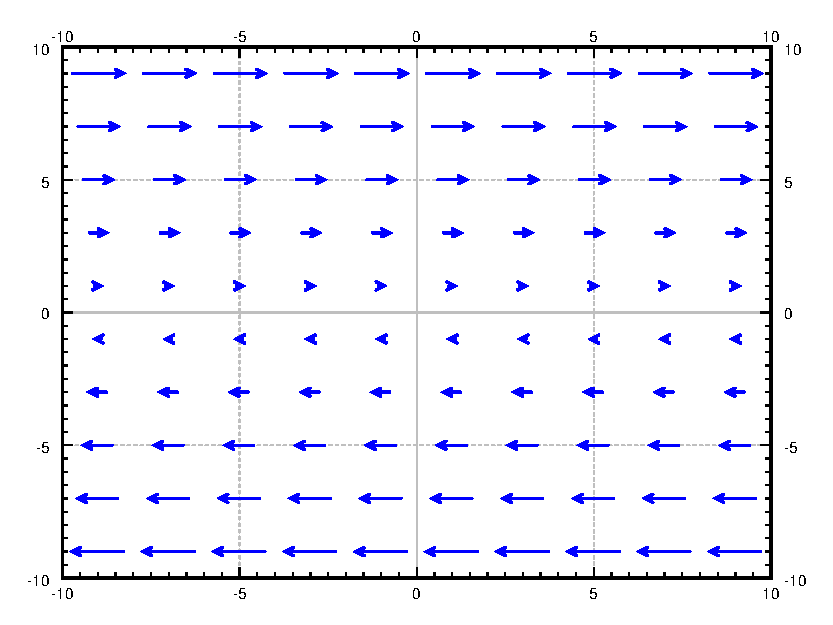
\includegraphics[width=2in]{figures/0100vectorfield}
\\
The solution will not move anywhere if $y = 0$.  When $y$ is positive,
then the solution moves (with constant speed)
in the positive $x$ direction.  When $y$ is
negative, then the solution moves (with constant speed) in the negative
$x$ direction.  It is not one of the behaviors we have seen.
\\
Note that the matrix has a double eigenvalue 0 and the general solution is
$x = C_1 t + C_2$ and $y = C_1$, which agrees with the above
description.
}

%%%%%%%%%%%%%%%%%%%%%%%%%%%%%%%%%%%%%%%%%%%%%%%%%%%%%%%%%%%%%%%%%%%%%%%%%%%%%%

\sectionnewpage
\section{Second order systems and applications}
\label{sol:section}

\sectionnotes{more than 2 lectures\EPref{, \S5.3 in \cite{EP}}\BDref{,
not in \cite{BD}}}

\subsection{Undamped mass-spring systems}

While we did say that we will usually only look at first order systems, it is
sometimes more convenient to study the system in the way it arises naturally.
For example, suppose we have 3 masses connected by springs between two
walls.  We could pick any higher number, and the math would be essentially
the same, but for simplicity we pick 3 right now.  Let us also assume no
friction, that is, the system is undamped\index{undamped motion!systems}.
The masses are $m_1$, $m_2$, and
$m_3$ and the spring constants are $k_1$, $k_2$, $k_3$, and $k_4$.
Let $x_1$ be the displacement from rest position of the first mass, and
$x_2$ and $x_3$ the displacement of the second and third mass.  We make,
as usual, positive values go right (as $x_1$ grows, the first mass is
moving right).
See \figurevref{sosa:threecartsfig}.

\begin{myfig}
\capstart
\inputpdft{threecartsfig}
\caption{System of masses and springs.\label{sosa:threecartsfig}}
\end{myfig}

This simple system turns up in unexpected places.  For example, 
our world really consists of many small particles of matter interacting together.
When we try the above system with many more masses, we obtain a good approximation to
how an elastic material behaves.  By somehow taking a limit of
the number of masses going to infinity, we obtain the continuous one
dimensional wave equation (that we study in \sectionref{we:section}).
But we digress.

Let us set up the equations for the \myindex{three mass system}.
By \myindex{Hooke's law}, the force acting on the mass equals the 
spring compression times the spring constant.  By
\myindex{Newton's second law},
force is mass times acceleration.  So if we sum the forces acting
on each mass, put the right sign in front of each term, depending on the
direction in which it is acting, and set this equal to mass
times the acceleration, we end up with the desired system of
equations.
\begin{equation*}
\begin{aligned}
m_1 x_1'' &= -k_1 x_1 + k_2 (x_2-x_1)
& & = -(k_1+k_2) x_1 + k_2 x_2 , \\
m_2 x_2'' &= -k_2 (x_2-x_1) + k_3 (x_3-x_2)
& & = k_2 x_1 -(k_2+k_3) x_2 + k_3 x_3 , \\
m_3 x_3'' &= -k_3 (x_3-x_2) - k_4 x_3
& & = k_3 x_2 - (k_3+k_4) x_3 . 
\end{aligned}
\end{equation*}
We define the matrices
\begin{equation*}
M =
\begin{bmatrix}
m_1 & 0 & 0 \\
0 & m_2 & 0 \\
0 & 0 & m_3
\end{bmatrix}
\qquad
\text{and}
\qquad
K =
\begin{bmatrix}
-(k_1+k_2) & k_2 & 0 \\
k_2 & -(k_2+k_3) & k_3 \\
0 & k_3 & -(k_3+k_4)
\end{bmatrix} .
\end{equation*}
We write the equation simply as
\begin{equation*}
M {\vec{x}}'' = K \vec{x} .
\end{equation*}
At this point we could introduce 3 new variables and write out a system
of 6 first order equations.  We claim this simple setup is easier to handle as
a second order system.
We call $\vec{x}$ the \emph{\myindex{displacement vector}}, $M$ the
\emph{\myindex{mass matrix}}, and $K$ the \emph{\myindex{stiffness matrix}}.

\begin{exercise}
Repeat this setup for 4 masses (find the matrices $M$ and $K$).
Do it for 5 masses.  Can you
find a prescription to do it for $n$ masses?
\end{exercise}

As with a single equation we want to \myquote{divide by $M$.}  This means
computing the inverse of $M$.
The masses are all nonzero and $M$ is a
diagonal matrix\index{diagonal matrix}, so computing the inverse
is easy:
\begin{equation*}
M^{-1} =
\begin{bmatrix}
\frac{1}{m_1} & 0 & 0 \\
0 & \frac{1}{m_2} & 0 \\
0 & 0 & \frac{1}{m_3}
\end{bmatrix} .
\end{equation*}
This fact follows readily
by how we multiply diagonal matrices.  As an exercise, you should verify that
$M M^{-1} = M^{-1} M = I$.

\medskip

Let $A = M^{-1}K$.  We look at the system
${\vec{x}}'' = M^{-1}K \vec{x}$, or
\begin{equation*}
{\vec{x}}'' = A \vec{x} .
\end{equation*}
Many real world systems can be modeled by this equation.  For simplicity,
we will only talk about the
given masses-and-springs problem.  We try a solution of the form
\begin{equation*}
\vec{x} = \vec{v} e^{\alpha t} .
\end{equation*}
We compute that for this guess,
${\vec{x}}'' = \alpha^2 \vec{v} e^{\alpha t}$.
We plug our guess into the equation and get
\begin{equation*}
\alpha^2 \vec{v} e^{\alpha t} = A\vec{v} e^{\alpha t} .
\end{equation*}
We divide by $e^{\alpha t}$ to arrive at
$\alpha^2 \vec{v} = A\vec{v}$.  Hence if $\alpha^2$ is an eigenvalue
of $A$ and $\vec{v}$ is a corresponding eigenvector, we have found
a solution.

In our example, and in other common applications,
$A$ has only real negative
eigenvalues (and possibly a zero eigenvalue).  So we study only this
case.  When an eigenvalue $\lambda$ is negative, it means that
$\alpha^2 = \lambda$ is negative.  Hence there is some real number $\omega$
such that $-\omega^2 = \lambda$.  Then $\alpha = \pm i \omega$.
The solution we guessed was
\begin{equation*}
\vec{x} = \vec{v} \, \bigl(\cos (\omega t) + i \sin (\omega t) \bigr) .
\end{equation*}
By taking the real and imaginary parts (note that $\vec{v}$ is real), we
find that 
$\vec{v} \cos (\omega t)$ and
$\vec{v} \sin (\omega t)$ are linearly independent solutions.

If an eigenvalue is zero, it turns out that both $\vec{v}$ and $\vec{v} t$ are
solutions, where $\vec{v}$ is an eigenvector corresponding to the eigenvalue
0.

\begin{exercise}
Show that if $A$ has a zero eigenvalue and $\vec{v}$ is a
corresponding eigenvector, then $\vec{x} = \vec{v} (a + bt)$ is a solution
of ${\vec{x}}'' = A \vec{x}$ for
arbitrary constants $a$ and $b$.
\end{exercise}

\begin{theorem}
Let $A$ be a real $n \times n$ matrix
with $n$ distinct real negative (or zero) eigenvalues we
denote by $-\omega_1^2 > -\omega_2^2 > \cdots > -\omega_n^2$, and
corresponding
eigenvectors by
$\vec{v}_1$, $\vec{v}_2$, \ldots, $\vec{v}_n$.  If $A$ is invertible
(that is, if $\omega_1 > 0$), then
\begin{equation*}
\boxed{~~
\vec{x}(t)
= \sum_{i=1}^n \vec{v}_i \bigl(a_i \cos (\omega_i t) + b_i \sin (\omega_i t) \bigr) ,
~~}
\end{equation*}
is the general solution of
\begin{equation*}
{\vec{x}}'' = A \vec{x},
\end{equation*}
for some arbitrary constants $a_i$ and $b_i$.
If $A$ has a zero eigenvalue, that is $\omega_1 = 0$,
and all other eigenvalues are distinct and
negative, then the general solution can be written as
\begin{equation*}
\boxed{~~
\vec{x}(t) = \vec{v}_1 (a_1 + b_1 t) +
\sum_{i=2}^n \vec{v}_i \bigl(a_i \cos (\omega_i t) + b_i \sin (\omega_i t) \bigr) .
~~}
\end{equation*}
\end{theorem}

We use this solution and the setup from the introduction
of this section even when some of the masses and springs are missing.  
For example, when there are only 2 masses and only 2 springs, simply take
only the equations for
the two masses and set all the spring constants for the springs that
are missing to zero.

\subsection{Examples}

\begin{example}
Consider the setup in \figurevref{sosa:twocartswallfig}, with
$m_1 = \unit[2]{kg}$, $m_2 = \unit[1]{kg}$, $k_1 = \unitfrac[4]{N}{m}$, and
$k_2 = \unitfrac[2]{N}{m}$.

\begin{myfig}
\capstart
\inputpdft{twocartswallfig}
\caption{System of masses and springs.\label{sosa:twocartswallfig}}
\end{myfig}

The equations we write down are
\begin{equation*}
\begin{bmatrix}
2 & 0 \\
0 & 1
\end{bmatrix}
{\vec{x}}'' =
\begin{bmatrix}
-(4+2) & 2 \\
2 & -2
\end{bmatrix}
\vec{x} ,
\end{equation*}
or
\begin{equation*}
{\vec{x}}'' =
\begin{bmatrix}
-3 & 1 \\
2 & -2
\end{bmatrix}
\vec{x} .
\end{equation*}

We find the eigenvalues of $A$ to be $\lambda = -1, -4$ (exercise).
We find corresponding eigenvectors to be
$\left[ \begin{smallmatrix} 1 \\ 2 \end{smallmatrix} \right]$ and
$\left[ \begin{smallmatrix} 1 \\ -1 \end{smallmatrix} \right]$ respectively
(exercise).

We check the theorem and note that $\omega_1 = 1$ and $\omega_2 = 2$.
Hence the general solution is
\begin{equation*}
\vec{x} = 
\begin{bmatrix} 1 \\ 2 \end{bmatrix}
\bigl( a_1 \cos (t) + b_1 \sin (t) \bigr)
+
\begin{bmatrix} 1 \\ -1 \end{bmatrix}
\bigl( a_2 \cos (2t) + b_2 \sin (2t) \bigr) .
\end{equation*}

The two terms in the solution represent the two
so-called \emph{natural\index{natural mode of oscillation}}
or \emph{normal modes of oscillation\index{normal mode of oscillation}}.
And the two (angular) frequencies are the
\emph{natural frequencies\index{natural frequency}}.
The first natural frequency is 1, and second natural frequency is 2.
The two modes are plotted in \figurevref{sosa:modesfig}.

\begin{myfig}
\capstart
%original files sosa-mode1 sosa-mode2
\diffyincludegraphics{width=6.24in}{width=9in}{sosa-modes-1-2}
\caption{The two modes of the mass-spring system.  In the left plot
the masses are moving in unison and in the right plot are masses moving in the
opposite direction.\label{sosa:modesfig}}
\end{myfig}

Let us write the solution as
\begin{equation*}
\vec{x} = 
\begin{bmatrix} 1 \\ 2 \end{bmatrix}
c_1 \cos (t - \alpha_1 )
+
\begin{bmatrix} 1 \\ -1 \end{bmatrix}
c_2 \cos (2t - \alpha_2 ) .
\end{equation*}
The first term,
\begin{equation*}
\begin{bmatrix} 1 \\ 2 \end{bmatrix}
c_1 \cos (t - \alpha_1 )
=
\begin{bmatrix}
c_1 \cos (t - \alpha_1 ) \\
2c_1 \cos (t - \alpha_1 )
\end{bmatrix} ,
\end{equation*}
corresponds to the mode where the masses move synchronously
in the same direction.

The second term,
\begin{equation*}
\begin{bmatrix} 1 \\ -1 \end{bmatrix}
c_2 \cos (2t - \alpha_2 )
=
\begin{bmatrix}
c_2 \cos (2t - \alpha_2 ) \\
- c_2 \cos (2t - \alpha_2 )
\end{bmatrix} ,
\end{equation*}
corresponds to the mode where the masses move synchronously
but in opposite directions.

The general solution is a combination of the two modes.  That is, the
initial conditions determine the amplitude and phase shift of each mode.
As an example, suppose we have initial conditions
\begin{equation*}
\vec{x}(0) = 
\begin{bmatrix} 1 \\ -1 \end{bmatrix}
, \qquad
\vec{x}'(0) = 
\begin{bmatrix} 0 \\ 6 \end{bmatrix} .
\end{equation*}
We use the $a_j, b_j$ constants to solve for initial conditions.  First
\begin{equation*}
\begin{bmatrix} 1 \\ -1 \end{bmatrix}
=
\vec{x}(0) = 
\begin{bmatrix} 1 \\ 2 \end{bmatrix}
a_1
+
\begin{bmatrix} 1 \\ -1 \end{bmatrix}
a_2 
=
\begin{bmatrix} a_1+a_2 \\2a_1 - a_2 \end{bmatrix}
\end{equation*}
We solve (exercise) to find $a_1 = 0$, $a_2 = 1$.
To find the $b_1$ and $b_2$, we differentiate first:
\begin{equation*}
{\vec{x}}' = 
\begin{bmatrix} 1 \\ 2 \end{bmatrix}
\bigl( - a_1 \sin (t) + b_1 \cos (t) \bigr)
+
\begin{bmatrix} 1 \\ -1 \end{bmatrix}
\bigl( - 2a_2 \sin (2t) + 2 b_2 \cos (2t) \bigr) .
\end{equation*}
Now we solve:
\begin{equation*}
\begin{bmatrix} 0 \\ 6 \end{bmatrix}
=
{\vec{x}}'(0) = 
\begin{bmatrix} 1 \\ 2 \end{bmatrix}
b_1
+
\begin{bmatrix} 1 \\ -1 \end{bmatrix}
2 b_2
=
\begin{bmatrix} b_1+2b_2 \\ 2b_1-2b_2 \end{bmatrix} .
\end{equation*}
Again solve (exercise) to find  $b_1 = 2$, $b_2 = -1$.  So our solution is
\begin{equation*}
\vec{x} = 
\begin{bmatrix} 1 \\ 2 \end{bmatrix}
2 \sin (t)
+
\begin{bmatrix} 1 \\ -1 \end{bmatrix}
\bigl( \cos (2t) - \sin (2t) \bigr)
=
\begin{bmatrix}
2 \sin (t) + \cos(2t)- \sin(2t) \\
4 \sin (t) - \cos(2t) + \sin(2t)
\end{bmatrix} .
\end{equation*}
The graphs of the two displacements, $x_1$ and $x_2$ of the two carts is in
\figureref{sosa:superposfig}.
\begin{myfig}
\capstart
\diffyincludegraphics{width=3in}{width=4.5in}{sosa-superpos}
\caption{Superposition of the two modes given the initial
conditions.\label{sosa:superposfig}}
\end{myfig}
\end{example}

\begin{example} \label{sosa:railcarexample}
We have two toy rail
cars.  Car 1 of mass \unit[2]{kg} is traveling at \unitfrac[3]{m}{s}
towards the second
rail car of mass \unit[1]{kg}.  There is a bumper on the second rail car that
engages at the moment the cars hit (it connects to two cars)
and does not let go.
The bumper acts like a spring of spring constant $k=\unitfrac[2]{N}{m}$.
The second
car is 10 meters from a wall.  See \figurevref{sosa:railcarscrashfig}.

\begin{myfig}
\capstart
\inputpdft{railcarscrash}
\caption{The crash of two rail cars.\label{sosa:railcarscrashfig}}
\end{myfig}

We want to ask several questions.  At what time after the cars link does
impact with the wall happen?  What is the speed of car 2 when it hits the
wall?

OK\@, let us first set the system up.  Let $t=0$ be the time
when the two cars link up.  Let $x_1$ be the displacement of the first car
from the position at $t=0$, and let $x_2$ be the
displacement of the second car from its original location.  Then the
time when $x_2(t) = 10$ is exactly the time when impact with wall occurs.
For this $t$, $x_2'(t)$ is the speed at impact.  This system acts just like the
system of the previous example but without $k_1$.  Hence the equation is
\begin{equation*}
\begin{bmatrix}
2 & 0 \\
0 & 1
\end{bmatrix}
{\vec{x}}'' =
\begin{bmatrix}
-2 & 2 \\
2 & -2
\end{bmatrix}
\vec{x} ,
\end{equation*}
or
\begin{equation*}
{\vec{x}}'' =
\begin{bmatrix}
-1 & 1 \\
2 & -2
\end{bmatrix}
\vec{x} .
\end{equation*}

We compute the eigenvalues of $A$.  It is not hard to see that the eigenvalues
are 0 and $-3$ (exercise).  Furthermore,
eigenvectors are
$\left[ \begin{smallmatrix} 1 \\ 1 \end{smallmatrix} \right]$ and
$\left[ \begin{smallmatrix} 1 \\ -2 \end{smallmatrix} \right]$ respectively
(exercise). 
Then
$\omega_1 = 0$,
$\omega_2 = \sqrt{3}$, and by the second part of the theorem
the general solution is
\begin{equation*}
\begin{split}
\vec{x} & = 
\begin{bmatrix} 1 \\ 1 \end{bmatrix}
\left( a_1 + b_1 t \right) 
+
\begin{bmatrix} 1 \\ -2 \end{bmatrix}
\left( a_2 \cos ( \sqrt{3} \, t) + b_2 \sin ( \sqrt{3} \, t ) \right)
\\
& =
\begin{bmatrix}
a_1 + b_1 t + a_2 \cos ( \sqrt{3} \, t ) + b_2 \sin ( \sqrt{3} \, t
) \\
a_1 + b_1 t - 2 a_2 \cos ( \sqrt{3} \, t ) - 2 b_2 \sin ( \sqrt{3}
\, t ) 
\end{bmatrix} .
\end{split}
\end{equation*}

We now apply the initial conditions.  First the cars start at position 0
so $x_1 (0) = 0$ and $x_2(0) = 0$.  The first car is traveling at
\unitfrac[3]{m}{s},
so $x_1'(0) = 3$ and the second car starts at rest, so $x_2'(0) = 0$.
The first conditions says
\begin{equation*}
\vec{0} = \vec{x}(0) = 
\begin{bmatrix}
a_1 + a_2 \\
a_1 - 2 a_2 
\end{bmatrix} .
\end{equation*}
It is not hard to see that $a_1 = a_2 = 0$.  We set $a_1=0$
and $a_2=0$ in $\vec{x}(t)$
and differentiate to get
\begin{equation*}
{\vec{x}}'(t)
=
\begin{bmatrix}
b_1 + \sqrt{3} \, b_2 \cos ( \sqrt{3} \, t ) \\
b_1 - 2 \sqrt{3} \, b_2 \cos ( \sqrt{3} \, t )
\end{bmatrix} .
\end{equation*}
So
\begin{equation*}
\begin{bmatrix} 3 \\ 0 \end{bmatrix} = 
{\vec{x}}'(0)
=
\begin{bmatrix}
b_1 + \sqrt{3} \, b_2 \\
b_1 - 2 \sqrt{3} \, b_2 
\end{bmatrix} .
\end{equation*}
Solving these two equations we
find $b_1 = 2$ and $b_2 =
\frac{1}{\sqrt{3}}$.  Hence the position of our cars is
(until the impact with the wall)
\begin{equation*}
\vec{x} = 
\begin{bmatrix}
2 t + \frac{1}{\sqrt{3}} \sin ( \sqrt{3} \, t ) \\
2 t - \frac{2}{\sqrt{3}} \sin ( \sqrt{3} \, t )
\end{bmatrix} .
\end{equation*}
Note how the presence of the zero eigenvalue resulted in a term containing $t$.
This means that the cars will be traveling in the positive direction as
time grows, which is what we expect.


What we are really interested in is the second expression, the one for $x_2$.
We have $x_2(t) = 
2 t - \frac{2}{\sqrt{3}} \sin ( \sqrt{3} \, t)$.  See \figurevref{sosa:railcarfig}
for the plot of $x_2$ versus time.

Just from the graph we can see that time of impact will be a little
more than 5 seconds from time zero.  For this we have to solve
the equation $10 = x_2(t) = 2 t - \frac{2}{\sqrt{3}} \sin ( \sqrt{3} \,
t)$.
Using a computer (or even a graphing calculator)
we find that $t_{\text{impact}} \approx 5.22$ seconds.

\begin{mywrapfig}{3.25in}
\capstart
\diffyincludegraphics{width=3in}{width=4.5in}{sosa-railcar}
\caption{Position of the second car in time (ignoring the wall).\label{sosa:railcarfig}}
\end{mywrapfig}


The speed of the second car is $x_2' = 2 - 2 \cos ( \sqrt{3} \, t)$.
At the time of impact (5.22 seconds from $t=0$) we get 
$x_2'(t_{\text{impact}}) \approx 3.85$.
%
The maximum speed is the maximum of $2 - 2 \cos ( \sqrt{3} \, t )$, which is 4.
We are traveling at almost the maximum speed when we hit the wall.

\medskip

Suppose that Bob is a tiny person sitting on car 2.  Bob has a Martini in
his hand and would like not to spill it.  Let us suppose Bob would not spill
his Martini
when the first car links up with car 2, but if car 2 hits the wall at any
speed greater than zero, Bob will spill his drink.  Suppose Bob
can move car 2
a few meters towards or away from the wall (he cannot go all the way to the
wall, nor can he get out of the way of the first car).  Is there a
\myquote{safe}
distance for him to be at?  A distance such that the impact with
the wall is at zero speed?

The answer is yes.  Looking at \figurevref{sosa:railcarfig},
we note the \myquote{plateau} between $t=3$ and $t=4$.  There is a point where
the speed is zero.  To find it we solve $x_2'(t) = 0$.  This is when
$\cos ( \sqrt{3} \, t) = 1$ or in other words when $t = \frac{2 \pi}{\sqrt{3}}, 
\frac{4 \pi}{\sqrt{3}},\ldots$ and so on.  We plug in the first value to obtain
$x_2\left(\frac{2 \pi}{\sqrt{3}}\right) = 
\frac{4 \pi}{\sqrt{3}} \approx 7.26$.  So a \myquote{safe} distance is about 7 and a
quarter meters from the wall.

Alternatively Bob could move away from the wall
towards the incoming car 2, where another safe distance is
$x_2 \left( \frac{4 \pi}{\sqrt{3}} \right) = \frac{8 \pi}{\sqrt{3}}
\approx 14.51$ and so on.  We can use all the different
$t$ such that $x_2'(t) = 0$.  Of course $t=0$ is always a solution here,
corresponding to $x_2 = 0$, but
that means standing right at the wall.
\end{example}

\subsection{Forced oscillations}

Finally we move to forced oscillations\index{forced motion!systems}.
Suppose that now our system is
\begin{equation} \label{sosa:forcedeq}
{\vec{x}}'' = A \vec{x} + \vec{F} \cos ( \omega t) .
\end{equation}
That is, we are adding periodic forcing to the system in the direction of
the vector $\vec{F}$.

As before, this system just requires us to find one particular solution
$\vec{x}_p$, add it to the general solution of the associated homogeneous system
$\vec{x}_c$, and we will have the general solution to \eqref{sosa:forcedeq}.
Let us suppose that $\omega$ is not one of the natural frequencies of
${\vec{x}}'' = A \vec{x}$, then we can guess
\begin{equation*}
\vec{x}_p = \vec{c} \cos (\omega t) ,
\end{equation*}
where $\vec{c}$ is an unknown constant vector.  Note that we do not need
to use sine since there are only second derivatives.  We solve for $\vec{c}$ to
find $\vec{x}_p$.  This is really just the method of
\emph{undetermined coefficients\index{undetermined coefficients!for second
order systems}}
for systems.  Let us differentiate $\vec{x}_p$ twice to get
\begin{equation*}
{\vec{x}_p}'' = -\omega^2 \vec{c} \cos (\omega t) .
\end{equation*}
Plug $\vec{x}_p$ and ${\vec{x}_p}''$ into equation \eqref{sosa:forcedeq}:
\begin{equation*}
\overbrace{
-\omega^2 \vec{c} \cos (\omega t)
}^{{\vec{x}_p}''}
=
\overbrace{
A \vec{c} \cos (\omega t) 
}^{A \vec{x}_p}
+ \vec{F} \cos (\omega t) .
\end{equation*}
We cancel out the cosine and rearrange the equation to obtain
\begin{equation*}
(A +\omega^2 I) \vec{c}
=
- \vec{F} .
\end{equation*}
So
\begin{equation*}
\vec{c}
=
{(A +\omega^2 I)}^{-1}
(-\vec{F} ).
\end{equation*}
Of course this is possible only if
$(A+ \omega^2 I) = \bigl(A- (-\omega^2) I\bigr)$ is
invertible.  That matrix is invertible if and only if
$-\omega^2$ is not an eigenvalue of $A$.  That is true if and only if $\omega$
is not a natural frequency of the system.

We simplified things a little bit.  If we wish to have the
forcing term to be in the units of force, say Newtons, then we must write
\begin{equation*}
M \vec{x}'' = K \vec{x} + \vec{G} \cos(\omega t) .
\end{equation*}
If we then write things in terms of $A = M^{-1} K$, we have
\begin{equation*}
\vec{x}'' = M^{-1}K \vec{x} + M^{-1} \vec{G} \cos(\omega t) 
\qquad \text{or} \qquad
\vec{x}'' = A \vec{x} + \vec{F} \cos(\omega t) ,
\end{equation*}
where $\vec{F} = M^{-1} \vec{G}$.

\begin{example}
Let us take the example in \figurevref{sosa:twocartswallfig} with
the same parameters as before:
$m_1 = 2$, $m_2 = 1$, $k_1 = 4$, and $k_2 = 2$.  Now suppose that
there is a force $2 \cos (3t)$ acting on the second cart.

The equation is
\begin{equation*}
\begin{bmatrix}
2 & 0 \\
0 & 1
\end{bmatrix}
{\vec{x}}'' =
\begin{bmatrix}
-4 & 2 \\
2 & -2
\end{bmatrix}
\vec{x} 
+ 
\begin{bmatrix}
0 \\ 2
\end{bmatrix}
\cos (3 t) \qquad \text{or} \qquad
{\vec{x}}'' =
\begin{bmatrix}
-3 & 1 \\
2 & -2
\end{bmatrix}
\vec{x} 
+ 
\begin{bmatrix}
0 \\ 2
\end{bmatrix}
\cos (3 t) .
\end{equation*}
We solved the associated homogeneous equation before and found the
complementary solution to be
\begin{equation*}
\vec{x}_c =
\begin{bmatrix} 1 \\ 2 \end{bmatrix}
\bigl( a_1 \cos (t) + b_1 \sin (t) \bigr)
+
\begin{bmatrix} 1 \\ -1 \end{bmatrix}
\bigl( a_2 \cos (2t) + b_2 \sin (2t) \bigr) .
\end{equation*}

The natural frequencies are 1 and 2.  As 3 is not a
natural frequency, we try $\vec{c} \cos (3t)$.
We invert $(A+3^2 I)$:
\begin{equation*}
{\left( \begin{bmatrix}
-3 & 1 \\
\noalign{\smallskip}
2 & -2
\end{bmatrix}
+3^2 I\right)}^{-1}
=
{\begin{bmatrix}
6 & 1 \\
\noalign{\smallskip}
2 & 7
\end{bmatrix}}^{-1}
=
\begin{bmatrix}
\frac{7}{40} & \frac{-1}{40} \\
\noalign{\smallskip}
\frac{-1}{20} & \frac{3}{20}
\end{bmatrix} .
\end{equation*}
Hence,
\begin{equation*}
\vec{c} = 
{(A +\omega^2 I)}^{-1}
(-\vec{F} ) = 
\begin{bmatrix}
\frac{7}{40} & \frac{-1}{40} \\
\noalign{\smallskip}
\frac{-1}{20} & \frac{3}{20}
\end{bmatrix}
\begin{bmatrix}
0 \\
\noalign{\smallskip}
-2
\end{bmatrix}
=
\begin{bmatrix}
\frac{1}{20} \\
\noalign{\smallskip}
\frac{-3}{10}
\end{bmatrix} .
\end{equation*}

Combining with the general solution of the associated
homogeneous problem, we get that the general solution to
${\vec{x}}'' = A \vec{x} + \vec{F} \cos (\omega t)$ is
\begin{equation*}
\vec{x} = \vec{x}_c + \vec{x}_p =
\begin{bmatrix} 1 \\
\noalign{\smallskip}
2 \end{bmatrix}
\bigl( a_1 \cos (t) + b_1 \sin (t) \bigr)
+
\begin{bmatrix} 1 \\
\noalign{\smallskip}
-1 \end{bmatrix}
\bigl( a_2 \cos (2t) + b_2 \sin (2t) \bigr)
+
\begin{bmatrix}
\frac{1}{20} \\
\noalign{\smallskip}
\frac{-3}{10}
\end{bmatrix}
\cos (3t) .
\end{equation*}
We then solve for the constants
$a_1$, $a_2$, $b_1$, and $b_2$ using
any initial conditions we are given.
\end{example}

Note that given force $\vec{f}$, we write 
the equation as $M {\vec{x}}'' = K \vec{x} + \vec{f}$ to get the units
right. Then we write
${\vec{x}}'' = M^{-1}K \vec{x} + M^{-1}\vec{f}$.  The 
term $\vec{g} = M^{-1} \vec{f}$ in ${\vec{x}}'' = A \vec{x} + \vec{g}$ is in units of force
per unit mass.

If $\omega$ is a natural frequency of the system
\emph{\myindex{resonance}} may occur,
because we will have to try a particular solution of the form
\begin{equation*}
\vec{x}_p =
\vec{c} \, t \sin (\omega t) +
\vec{d} \, \cos (\omega t) .
\end{equation*}
That is assuming that the eigenvalues of the coefficient matrix are distinct.
Next, note that the amplitude of this solution grows without bound as $t$ grows.

\subsection{Exercises}

\begin{exercise}
Find a particular solution to
\begin{equation*}
{\vec{x}}'' =
\begin{bmatrix}
-3 & 1 \\
2 & -2
\end{bmatrix}
\vec{x} 
+ 
\begin{bmatrix}
0 \\ 2
\end{bmatrix}
\cos (2 t) .
\end{equation*}
\end{exercise}

\begin{exercise}[challenging]
Let us take the example in \figurevref{sosa:twocartswallfig} with
the same parameters as before:
$m_1 = 2$, $k_1 = 4$, and $k_2 = 2$, except for $m_2$, which is unknown.
Suppose that there is a force $\cos (5 t)$ acting on the first mass.
Find an $m_2$ such that there exists a particular solution where the
first mass does not move.

Note: This idea is called \emph{\myindex{dynamic damping}}.
In practice there will be a small amount of
damping and so any transient solution will disappear and after long enough
time, the first mass will always come to a stop.
\end{exercise}

\begin{exercise}
Let us take the \examplevref{sosa:railcarexample}, but that at
time of impact, car 2 is moving to the left at the speed of
\unitfrac[3]{m}{s}.  a)
Find the behavior of the system after linkup.  b) Will the second car hit
the wall, or will it be moving away from the wall as time goes on?  c) At
what speed would the first car have to be traveling for the system to
essentially stay in place after linkup?
\end{exercise}

\begin{exercise}
Let us take the example in \figurevref{sosa:twocartswallfig} with
parameters
$m_1 = m_2 = 1$, $k_1 = k_2 = 1$.  Does there exist a set of initial
conditions for which the first cart moves but the second cart does not?
If so, find those conditions.  If not, argue why not.
\end{exercise}

\setcounter{exercise}{100}

\begin{exercise}
Find the general solution to
$\left[ \begin{smallmatrix}
1 & 0 & 0\\
0 & 2 & 0\\
0 & 0 & 3
\end{smallmatrix}\right]
\vec{x}\,''
=
\left[ \begin{smallmatrix}
-3 & 0 & 0 \\
2 & -4 & 0 \\
0 & 6 & -3
\end{smallmatrix}\right]
\vec{x}
+ 
\left[ \begin{smallmatrix}
\cos(2t) \\ 0 \\ 0
\end{smallmatrix}\right]$.
\end{exercise}
\exsol{%
$\vec{x}
=
\left[ \begin{smallmatrix}
1 \\ -1 \\ 1
\end{smallmatrix}\right]
\bigl( a_1 \cos (\sqrt{3}\, t)  + b_1 \sin (\sqrt{3}\, t) \bigr)
+
\left[ \begin{smallmatrix}
0 \\ 1 \\ -2
\end{smallmatrix}\right]
\bigl( a_2 \cos (\sqrt{2}\, t)  + b_2 \sin (\sqrt{2}\, t) \bigr)
+
$
\\
$
\left[ \begin{smallmatrix}
0 \\ 0 \\ 1
\end{smallmatrix}\right]
\bigl( a_3 \cos (t)  + b_3 \sin (t) \bigr)
+
\left[ \begin{smallmatrix}
-1 \\ \nicefrac{1}{2} \\ \nicefrac{2}{3}
\end{smallmatrix}\right]
\cos (2t)$
}

\begin{exercise}
Suppose there are three carts of equal mass $m$ and connected by two springs of
constant $k$ (and no connections to walls).  Set up the system and find its
general solution.
\end{exercise}
\exsol{%
$\left[ \begin{smallmatrix}
m & 0 & 0\\
0 & m & 0\\
0 & 0 & m
\end{smallmatrix}\right]
\vec{x}\,''
=
\left[ \begin{smallmatrix}
-k & k & 0 \\
k & -2k & k \\
0 & k & -k
\end{smallmatrix}\right]
\vec{x}$.
Solution:
$\vec{x} =
\left[ \begin{smallmatrix}
1 \\ -2 \\ 1
\end{smallmatrix}\right]
\bigl( a_1 \cos (\sqrt{\nicefrac{3k}{m}}\, t)  + b_1 \sin
(\sqrt{\nicefrac{3k}{m}}\, t) \bigr)
+
\left[ \begin{smallmatrix}
1 \\ 0 \\ -1
\end{smallmatrix}\right]
\bigl( a_2 \cos (\sqrt{\nicefrac{k}{m}}\, t)  + b_2 \sin
(\sqrt{\nicefrac{k}{m}}\, t) \bigr)
+
\left[ \begin{smallmatrix}
1 \\ 1 \\ 1
\end{smallmatrix}\right]
\bigl( a_3 t  + b_3 \bigr).$
}

\begin{exercise}
Suppose a cart of mass \unit[2]{kg} is attached by a spring of
constant $k=1$ to a cart of mass \unit[3]{kg}, which
is attached to the wall by a spring also of constant $k=1$.
Suppose that the initial position of the first cart is 1 meter in the
positive direction from the rest position, and the second mass starts at the
rest position.  The masses are not moving and are let go.  Find the
position of the second mass as a function of time.
\end{exercise}
\exsol{%
$x_2 =
( \nicefrac{2}{5} )
\cos (\sqrt{\nicefrac{1}{6}}\, t)
-
( \nicefrac{2}{5} )
\cos (t)$
%sol
%$\vec{x} =
%\left[ \begin{smallmatrix}
%3 \\ 2
%\end{smallmatrix}\right]
%\bigl( a_1 \cos (\sqrt{\nicefrac{1}{6}}\, t)  + b_1 \sin
%(\sqrt{\nicefrac{1}{6}}\, t) \bigr)
%+
%\left[ \begin{smallmatrix}
%1 \\ -1
%\end{smallmatrix}\right]
%\bigl( a_2 \cos (t)  + b_2 \sin (t) \bigr)$.
}

%%%%%%%%%%%%%%%%%%%%%%%%%%%%%%%%%%%%%%%%%%%%%%%%%%%%%%%%%%%%%%%%%%%%%%%%%%%%%%

\sectionnewpage
\section{Multiple eigenvalues} \label{sec:multeigen}

\sectionnotes{1 or 1.5 lectures\EPref{, \S5.4 in \cite{EP}}\BDref{,
\S7.8 in \cite{BD}}}

It may happen that a matrix $A$ has some \myquote{repeated} eigenvalues.
That is, the characteristic equation $\det(A-\lambda I) = 0$ may have
repeated roots.  As we said before, this is actually unlikely to happen
for a random matrix.  If we take a small perturbation of $A$ (we change the
entries of $A$ slightly), we get a matrix with distinct eigenvalues.  As
any system we want to solve in practice is an approximation to reality
anyway, it is not absolutely indispensable to know how to solve these corner cases.  
On the other hand, these cases do come up in applications from time to time.
Furthermore, if we have distinct but very close eigenvalues, the behavior is
similar to that of repeated eigenvalues, and so understanding that case
will give us insight into what is going on.

\subsection{Geometric multiplicity}

Take the diagonal matrix
\begin{equation*}
A =
\begin{bmatrix}
3 & 0 \\ 0 & 3
\end{bmatrix} .
\end{equation*}
$A$ has an eigenvalue 3 of multiplicity 2.  We call the
multiplicity of the eigenvalue\index{multiplicity of an eigenvalue}
in the characteristic equation the
\emph{\myindex{algebraic multiplicity}}.  In this case, there also exist 2
linearly
independent eigenvectors,
$\left[ \begin{smallmatrix} 1 \\ 0 \end{smallmatrix} \right]$
and
$\left[ \begin{smallmatrix} 0 \\ 1 \end{smallmatrix} \right]$ corresponding
to the eigenvalue 3.  This means
that the so-called \emph{\myindex{geometric multiplicity}}
of this eigenvalue is also 2.

In all the
theorems where we required a matrix to have $n$ distinct eigenvalues, we only
really needed to have $n$ linearly independent eigenvectors.  For example,
${\vec{x}}' = A\vec{x}$ has the general solution
\begin{equation*}
\vec{x} = 
c_1 \begin{bmatrix} 1 \\ 0 \end{bmatrix} e^{3t}
+ c_2 \begin{bmatrix} 0 \\ 1 \end{bmatrix} e^{3t} .
\end{equation*}
Let us restate the theorem about real eigenvalues.  In the following theorem
we will repeat eigenvalues according to (algebraic) multiplicity.  So
for the above matrix $A$, we would say that it has eigenvalues 3 and 3.

\begin{theorem}
Suppose the $n \times n$ matrix $P$ 
has $n$ real eigenvalues (not necessarily distinct), $\lambda_1$,
$\lambda_2$, \ldots, $\lambda_n$,
and there are $n$ linearly independent corresponding eigenvectors
$\vec{v}_1$, $\vec{v}_2$, \ldots, $\vec{v}_n$.  Then the general solution to 
${\vec{x}}' = P\vec{x}$
can be written as
\begin{equation*}
\vec{x} = c_1 \vec{v}_1 e^{\lambda_1 t} +
c_2 \vec{v}_2 e^{\lambda_2 t} + \cdots +
c_n \vec{v}_n e^{\lambda_n t} .
\end{equation*}
\end{theorem}

The \emph{geometric multiplicity} of an eigenvalue of algebraic multiplicity $n$
is equal to the number of corresponding linearly independent eigenvectors.
The geometric multiplicity is always less than or
equal to the algebraic multiplicity.  The theorem handles the case
when these two multiplicities are equal for all eigenvalues.
If for an eigenvalue the geometric multiplicity is equal
to the algebraic multiplicity, then we say the eigenvalue is
\emph{complete\index{complete eigenvalue}}.

In other words, 
the hypothesis of the theorem could be stated as saying that if all
the eigenvalues of $P$ are complete, then there are $n$ linearly independent
eigenvectors and thus we have the given general solution.

\medskip

If the geometric multiplicity of an eigenvalue is 2 or greater,
then the set of linearly independent eigenvectors is not unique up to
multiples as it was before.  For example, for the diagonal matrix $A =
\left[ \begin{smallmatrix} 3 & 0 \\ 0 & 3 \end{smallmatrix} \right]$
we could also pick eigenvectors
$\left[ \begin{smallmatrix} 1 \\ 1 \end{smallmatrix} \right]$
and
$\left[ \begin{smallmatrix} 1 \\ -1 \end{smallmatrix} \right]$, or in fact
any pair of two linearly independent vectors.  The number of linearly
independent eigenvectors corresponding to $\lambda$
is the number of free variables we obtain when solving $A\vec{v} =
\lambda \vec{v}$.  We pick specific values for those free variables to
obtain eigenvectors.  If you pick different values, you may get different
eigenvectors.


\subsection{Defective eigenvalues}

If an $n \times n$ matrix has less than $n$ linearly independent
eigenvectors, it is said to be \emph{deficient\index{deficient matrix}}.
Then there is at least
one eigenvalue with an algebraic multiplicity that is higher than its geometric
multiplicity.  We call this eigenvalue \emph{defective\index{defective
eigenvalue}}
and the difference
between the two multiplicities we call the \emph{\myindex{defect}}.

\begin{example}
The matrix
\begin{equation*}
\begin{bmatrix}
3 & 1 \\ 0 & 3
\end{bmatrix}
\end{equation*}
has an eigenvalue 3 of algebraic multiplicity 2.
Let us try to compute eigenvectors.
\begin{equation*}
\begin{bmatrix}
0 & 1 \\ 0 & 0
\end{bmatrix}
\begin{bmatrix}
v_1 \\ v_2
\end{bmatrix}
= \vec{0} .
\end{equation*}
We must have that $v_2 = 0$.  Hence any eigenvector is of the form
$\left[ \begin{smallmatrix} v_1 \\ 0 \end{smallmatrix} \right]$.  Any two
such vectors are linearly dependent, and hence the geometric multiplicity
of the eigenvalue is 1.  Therefore, the defect is 1, and we can no longer
apply the eigenvalue method directly to a system of ODEs with such a
coefficient matrix.

\medskip

Roughly, the key observation is that
if $\lambda$ is an eigenvalue of $A$ of algebraic multiplicity $m$,
then we can find certain $m$ linearly independent vectors
solving ${(A-\lambda I)}^k \vec{v} = \vec{0}$ for various powers
$k$.  We will call these \emph{\myindex{generalized eigenvectors}}.

\medskip

Let us continue with the example
$A = \left[ \begin{smallmatrix}
3 & 1 \\ 0 & 3
\end{smallmatrix} \right]$ and the equation ${\vec{x}}' = A\vec{x}$.
We found an eigenvalue $\lambda=3$ of (algebraic) multiplicity 2 and defect 1.
We found one eigenvector 
$\vec{v} = \left[ \begin{smallmatrix} 1 \\ 0 \end{smallmatrix} \right]$.
We have one solution
\begin{equation*}
\vec{x}_1 = \vec{v} e^{3t} = \begin{bmatrix} 1 \\ 0 \end{bmatrix} e^{3t} .
\end{equation*}
We are now stuck, we get no other solutions from standard eigenvectors.  But
we need two linearly independent solutions to find the general solution of
the equation.

Let us try (in the spirit of repeated roots of the
characteristic equation for a single equation) another solution of the form
\begin{equation*}
\vec{x}_2 = ( \vec{v}_2 +  \vec{v}_1 t )\, e^{3t} .
\end{equation*}
We differentiate to get
\begin{equation*}
{\vec{x}_2}' =
\vec{v}_1 e^{3t} +
3 ( \vec{v}_2 +  \vec{v}_1 t )\, e^{3t}
=
( 3 \vec{v}_2 + \vec{v}_1 )\, e^{3t} +  3 \vec{v}_1 t e^{3t} .
\end{equation*}
As we are assuming that $\vec{x}_2$ is a solution, ${\vec{x}_2}'$ must
equal $A \vec{x}_2$. So let's compute $A \vec{x}_2$:
\begin{equation*}
A \vec{x}_2 = 
A ( \vec{v}_2 +  \vec{v}_1 t )\, e^{3t}
=
A \vec{v}_2 e^{3t} +  A \vec{v}_1 t e^{3t} .
\end{equation*}
By looking at the coefficients of $e^{3t}$ and $t e^{3t}$ we see
$3 \vec{v}_2 + \vec{v}_1 = A \vec{v}_2$ and
$3 \vec{v}_1 = A \vec{v}_1$.
This means that
\begin{equation*}
(A-3I)\vec{v}_2 = \vec{v}_1,
\qquad \text{and} \qquad
(A-3I)\vec{v}_1 = \vec{0}.
\end{equation*}
Therefore, $\vec{x}_2$ is a solution
if these two equations are satisfied.
The second equation is satisfied if $\vec{v}_1$ is an
eigenvector, and we found the eigenvector above, so let
$\vec{v}_1 = 
\left[ \begin{smallmatrix} 1 \\ 0 \end{smallmatrix} \right]$.
So, if we can find a $\vec{v}_2$ that solves
%${(A-3I)}^2\vec{v}_2 = \vec{0}$ and such that
$(A-3I)\vec{v}_2 = \vec{v}_1$, then we are done.
This is just a bunch of linear
equations to solve and we are by now very good at that.
%
Let us solve
$(A-3I)\vec{v}_2 = \vec{v}_1$.  Write
\begin{equation*}
\begin{bmatrix}
0 & 1 \\ 0 & 0
\end{bmatrix}
\begin{bmatrix}
a \\ b
\end{bmatrix}
=
\begin{bmatrix}
1 \\ 0
\end{bmatrix} .
\end{equation*}
By inspection we see that letting $a=0$ ($a$ could be anything in fact) and
$b=1$ does the job.  Hence we can take $\vec{v}_2 = 
\left[ \begin{smallmatrix} 0 \\ 1 \end{smallmatrix} \right]$.  Our general
solution to
${\vec{x}}' = A\vec{x}$ is
\begin{equation*}
\vec{x} =
c_1 
\begin{bmatrix}
1 \\ 0
\end{bmatrix}
e^{3t}
+
c_2
\left(
\begin{bmatrix}
0 \\ 1
\end{bmatrix}
+
\begin{bmatrix}
1 \\ 0
\end{bmatrix}
t
\right)
\,
e^{3t}
=
\begin{bmatrix}
c_1 e^{3t}+c_2 te^{3t} \\
c_2 e^{3t}
\end{bmatrix} .
\end{equation*}
Let us check that we really do have the solution.  First
$x_1' = 
c_1 3 e^{3t}+c_2 e^{3t} + 3 c_2 te^{3t} = 3 x_1 + x_2$.  Good.  Now
$x_2' = 3 c_2 e^{3t} = 3x_2$.  Good.
\end{example}

In the example, if we plug $(A-3I)\vec{v}_2 = \vec{v}_1$ into
$(A-3I)\vec{v}_1 = \vec{0}$ we find
\begin{equation*}
(A-3I)(A-3I) \vec{v}_2 = \vec{0},
\qquad \text{or} \qquad
{(A-3I)}^2\vec{v}_2 = \vec{0}.
\end{equation*}
Furthermore, if 
$(A-3I) \vec{w} \not= \vec{0}$, then 
$(A-3I) \vec{w}$ is an eigenvector, a multiple of $\vec{v}_1$.
In this $2 \times 2$ case ${(A-3I)}^2$ is just the zero matrix (exercise).
So any vector $\vec{w}$ solves
${(A-3I)}^2\vec{w} = \vec{0}$ and we just need a $\vec{w}$ such that
$(A-3I)\vec{w} \not= \vec{0}$.  Then we could use
$\vec{w}$ for $\vec{v}_2$, and $(A-3I)\vec{w}$ for $\vec{v}_1$.

Note that the system ${\vec{x}}' = A \vec{x}$ has a simpler solution since
$A$ is a so-called \emph{\myindex{upper triangular matrix}}, that is
every entry below the diagonal is zero.
In particular, the equation for $x_2$
does not depend on $x_1$.  Mind you, not every defective matrix is
triangular.

\begin{exercise}
Solve ${\vec{x}}' = \left[ \begin{smallmatrix}
3 & 1 \\ 0 & 3
\end{smallmatrix} \right] \vec{x}$ by first solving for $x_2$ and then for
$x_1$ independently.  Check that you got the same solution as we did
above.
\end{exercise}

Let us describe the general algorithm.  Suppose that $\lambda$ is an
eigenvalue of multiplicity 2, defect 1.
First find an eigenvector $\vec{v}_1$ of $\lambda$.  
That is, $\vec{v}_1$ solves
$(A-\lambda I)\vec{v}_1  = \vec{0}$.
Then, find a vector $\vec{v}_2$ such that
\begin{equation*}
%{(A-\lambda I)}^2\vec{v}_2 & = \vec{0} , \\
(A-\lambda I)\vec{v}_2 = \vec{v}_1 .
\end{equation*}
This gives us two linearly independent solutions
\begin{align*}
\vec{x}_1 & = \vec{v}_1 e^{\lambda t} , \\
\vec{x}_2 & = \left( \vec{v}_2 + \vec{v}_1 t \right) e^{\lambda t} .
\end{align*}

\begin{example}
Consider the system
\begin{equation*}
\vec{x}' =
\begin{bmatrix}
2 & -5 & 0 \\
0 & 2 & 0 \\
-1 & 4 & 1
\end{bmatrix}
\vec{x} .
\end{equation*}
Compute the eigenvalues,
\begin{equation*}
0 =
\det(A-\lambda I) = 
\det\left(
\begin{bmatrix}
2-\lambda & -5 & 0 \\
0 & 2-\lambda & 0 \\
-1 & 4 & 1-\lambda
\end{bmatrix}
\right)
= (2-\lambda)^2(1-\lambda) .
\end{equation*}
So the eigenvalues are 1 and 2, where 2 has multiplicity 2.
For the eigenvalue $\lambda = 1$ we leave it to the reader to find that
$\left[ \begin{smallmatrix} 0 \\ 0 \\ 1 \end{smallmatrix} \right]$
is an eigenvector.

Let's focus on $\lambda = 2$.  Let's compute eigenvectors,
\begin{equation*}
\vec{0} =
(A - 2 I) \vec{v}
=
\begin{bmatrix}
0 & -5 & 0 \\
0 & 0 & 0 \\
-1 & 4 & -1
\end{bmatrix}
\begin{bmatrix}
v_1 \\ v_2 \\ v_3
\end{bmatrix}
.
\end{equation*}
The first equation says that $v_2 = 0$, so the last equation
is $-v_1 -v_3 = 0$.  Let $v_3$ be the free variable to find
that $v_1 = -v_3$.  Perhaps let $v_3 = -1$ to find an eigenvector
$\left[ \begin{smallmatrix} 1 \\ 0 \\ -1 \end{smallmatrix} \right]$.
Problem is that setting $v_3$ to anything else just gets multiples
of this vector and so we have a defect of 1.
Let $\vec{v}_1$ be the eigenvector and let's look for
a generalized eigenvector $\vec{v}_2$.
\begin{equation*}
(A - 2 I) \vec{v}_2 = \vec{v}_1 . 
\end{equation*}
or
\begin{equation*}
\begin{bmatrix}
0 & -5 & 0 \\
0 & 0 & 0 \\
-1 & 4 & -1
\end{bmatrix}
\begin{bmatrix}
a \\ b \\ c
\end{bmatrix}
=
\begin{bmatrix}
1 \\ 0 \\ -1
\end{bmatrix} ,
\end{equation*}
where we used $a$, $b$, $c$ as components of $\vec{v}_2$ for simplicity.
The first equation says $-5b = 1$ so $b = \nicefrac{-1}{5}$.  The
second equation says nothing.
The last equation is $-a + 4b - c = -1$ or
$a + \nicefrac{4}{5} + c = 1$ or
$a + c = \nicefrac{1}{5}$.  We can let $c$ be the free variable, so let's
choose $c=0$.  We find
$\vec{v}_2 = \left[ \begin{smallmatrix} \nicefrac{1}{5} \\ \nicefrac{-1}{5}
\\ 0 \end{smallmatrix} \right]$.

The general solution is therefore,
\begin{equation*}
\vec{x} =
c_1
\begin{bmatrix} 0 \\ 0 \\ 1 \end{bmatrix}
e^t
+
c_2 
\begin{bmatrix} 1 \\ 0 \\ -1 \end{bmatrix}
e^{2t}
+
c_3
\left(
\begin{bmatrix} \nicefrac{1}{5} \\ \nicefrac{-1}{5} \\ 0 \end{bmatrix}
+
\begin{bmatrix} 1 \\ 0 \\ -1 \end{bmatrix}
t
\right)
e^{2t}
.
\end{equation*}
\end{example}

This machinery can also be generalized to higher multiplicities
and higher defects.
We will not go over this method in detail, but let us just sketch the ideas.  Suppose that $A$
has an eigenvalue $\lambda$ of multiplicity $m$.
We find vectors such that
\begin{equation*}
{(A - \lambda I)}^k \vec{v} = \vec{0},
\qquad \text{but} \qquad
{(A - \lambda I)}^{k-1} \vec{v} \not= \vec{0}.
\end{equation*}
Such vectors are called \emph{\myindex{generalized eigenvectors}} (then
$\vec{v}_1 = {(A - \lambda I)}^{k-1} \vec{v}$ is an eigenvector).
For the
eigenvector $\vec{v}_1$ there is a chain of generalized eigenvectors
$\vec{v}_2$ through $\vec{v}_k$ such that:
\begin{align*}
(A - \lambda I) \vec{v}_1 & = \vec{0} , \\
(A - \lambda I) \vec{v}_2 & = \vec{v}_1 , \\
& ~~\vdots \\
(A - \lambda I) \vec{v}_k & = \vec{v}_{k-1} .
\end{align*}
Really once you find the $\vec{v}_k$ such that
${(A - \lambda I)}^k \vec{v}_k = \vec{0}$ but
${(A - \lambda I)}^{k-1} \vec{v}_k \not= \vec{0}$, you find the entire
chain since you can compute the rest,
$\vec{v}_{k-1} = (A - \lambda I) \vec{v}_k$,
$\vec{v}_{k-2} = (A - \lambda I) \vec{v}_{k-1}$, etc.
We form the linearly independent solutions
\begin{align*}
\vec{x}_1 & = \vec{v}_1 e^{\lambda t} , \\
\vec{x}_2 & = ( \vec{v}_2 + \vec{v}_1 t ) \, e^{\lambda t} , \\
& ~~\vdots \\
\vec{x}_k & = \left( \vec{v}_k + \vec{v}_{k-1} t +
\vec{v}_{k-2} \frac{t^2}{2} +
\cdots + \vec{v}_2 \frac{t^{k-2}}{(k-2)!} + \vec{v}_1 \frac{t^{k-1}}{(k-1)!}
\right) \, e^{\lambda t} .
\end{align*}
Recall that $k! = 1 \cdot 2 \cdot 3 \cdots (k-1) \cdot k$ is the factorial.
If you have an eigevalue of geometric multiplicity $\ell$,
you will have to find $\ell$ such chains (some of them might be
short: just the single eigenvector equation).
We go until we form $m$ linearly independent solutions where
$m$ is the algebraic multiplicity.
We don't quite know which specific eigenvectors go with which chain, so
start by finding $\vec{v}_k$ first for the longest possible chain and
go from there.

For example, if $\lambda$ is an eigenvalue of $A$
of algebraic multiplicity 3 and defect 2, then solve
\begin{equation*}
(A - \lambda I) \vec{v}_1 = \vec{0} , \qquad
(A - \lambda I) \vec{v}_2 = \vec{v}_1 , \qquad
(A - \lambda I) \vec{v}_3 = \vec{v}_2 .
\end{equation*}
That is, find $\vec{v}_3$ such that 
${(A - \lambda I)}^3 \vec{v}_3 = \vec{0}$, but
${(A - \lambda I)}^2 \vec{v}_3 \not= \vec{0}$.
Then you are done as
$\vec{v}_2 = (A - \lambda I) \vec{v}_3$
and 
$\vec{v}_1 = (A - \lambda I) \vec{v}_2$.
The 3 linearly independent solutions are
\begin{equation*}
\vec{x}_1 = \vec{v}_1 e^{\lambda t} , \qquad
\vec{x}_2 = ( \vec{v}_2 + \vec{v}_1 t ) \, e^{\lambda t} , \qquad
\vec{x}_3 = \left( \vec{v}_3 + \vec{v}_2 t +
\vec{v}_{1} \frac{t^2}{2} \right) \, e^{\lambda t} .
\end{equation*}

If on the other hand $A$ has an eigenvalue $\lambda$
of algebraic multiplicity 3 and defect 1, then 
solve
\begin{equation*}
(A - \lambda I) \vec{v}_1 = \vec{0} , \qquad
(A - \lambda I) \vec{v}_2 = \vec{0} , \qquad
(A - \lambda I) \vec{v}_3 = \vec{v}_2 .
\end{equation*}
Here $\vec{v}_1$ and $\vec{v}_2$ are actual honest eigenvectors,
and $\vec{v}_3$ is a generalized eigenvector.
So there are two chains.
To solve, first find a 
$\vec{v}_3$ such that 
${(A - \lambda I)}^2 \vec{v}_3 = \vec{0}$, but
$(A - \lambda I) \vec{v}_3 \not= \vec{0}$.
Then $\vec{v}_2 = (A - \lambda I) \vec{v}_3$ is going to be an eigenvector.
Then solve for an eigenvector $\vec{v}_1$ that is linearly independent 
from $\vec{v}_2$.
You get 3 linearly independent solutions
\begin{equation*}
\vec{x}_1 = \vec{v}_1 e^{\lambda t} , \qquad
\vec{x}_2 = \vec{v}_2 e^{\lambda t} , \qquad
\vec{x}_3 = ( \vec{v}_3 + \vec{v}_2 t ) \, e^{\lambda t} .
\end{equation*}

\subsection{Exercises}

\begin{exercise}
Let
$A = \left[ \begin{smallmatrix} 5 & -3 \\ 3 & -1 \end{smallmatrix} \right]$.
Find the general solution of ${\vec{x}}' = A \vec{x}$.
\end{exercise}

\begin{samepage}
\begin{exercise}
Let
$A = \left[ \begin{smallmatrix}
5 & -4 & 4 \\
0 & 3 & 0 \\
-2 & 4 & -1
\end{smallmatrix} \right]$.
\begin{enumerate}[a)]
\item What are the eigenvalues?
\item What is/are the defect(s) of the eigenvalue(s)?
\item Find the general solution of ${\vec{x}}' = A \vec{x}$.
\end{enumerate}
\end{exercise}
\end{samepage}


\begin{exercise}
Let
$A = \left[ \begin{smallmatrix} 2 & 1 & 0 \\ 0 & 2 & 0 \\ 0 & 0 & 2 \end{smallmatrix} \right]$.
\begin{enumerate}[a)]
\item What are the eigenvalues?
\item What is/are the defect(s) of the eigenvalue(s)?
\item Find the general solution of ${\vec{x}}' = A \vec{x}$ in two different
ways and verify you get the same answer.
\end{enumerate}
\end{exercise}

\begin{exercise}
Let
$A = \left[ \begin{smallmatrix}
0 & 1 & 2 \\
-1 & -2 & -2 \\
-4 & 4 & 7
\end{smallmatrix} \right]$.
\begin{enumerate}[a)]
\item What are the eigenvalues?
\item What is/are the defect(s) of the eigenvalue(s)?
\item Find the general solution of ${\vec{x}}' = A \vec{x}$.
\end{enumerate}
\end{exercise}

\begin{exercise}
Let
$A = \left[ \begin{smallmatrix}
0 & 4 & -2 \\
-1 & -4 & 1 \\
0 & 0 & -2
\end{smallmatrix} \right]$.
\begin{enumerate}[a)]
\item What are the eigenvalues?
\item What is/are the defect(s) of the eigenvalue(s)?
\item Find the general solution of ${\vec{x}}' = A \vec{x}$.
\end{enumerate}
\end{exercise}

\begin{exercise}
Let
$A = \left[ \begin{smallmatrix}
2 & 1 & -1 \\
-1 & 0 & 2 \\
-1 & -2 & 4
\end{smallmatrix} \right]$.
\begin{enumerate}[a)]
\item What are the eigenvalues?
\item What is/are the defect(s) of the eigenvalue(s)?
\item Find the general solution of ${\vec{x}}' = A \vec{x}$.
\end{enumerate}
\end{exercise}

\begin{exercise}
Suppose that $A$ is a $2 \times 2$ matrix with a repeated eigenvalue
$\lambda$.
Suppose that there are two linearly independent eigenvectors.  Show that
$A = \lambda I$.
\end{exercise}

\setcounter{exercise}{100}

\begin{exercise}
Let $A =
\left[ \begin{smallmatrix}
1 & 1 & 1 \\
1 & 1 & 1 \\
1 & 1 & 1 
\end{smallmatrix}\right]$.  
\begin{enumerate}[a)]
\item What are the eigenvalues?
\item What is/are the defect(s) of the eigenvalue(s)?
\item Find the general solution of $\vec{x}\,' = A\vec{x}$.
\end{enumerate}
\end{exercise}
\exsol{%
a) $3,0,0$
\quad
b) No defects.
\quad
c)
$\vec{x} =
C_1
\left[ \begin{smallmatrix}
1 \\ 1 \\ 1
\end{smallmatrix}\right]
e^{3t}
+
C_2
\left[ \begin{smallmatrix}
1 \\ 0 \\ -1
\end{smallmatrix}\right]
+
C_3
\left[ \begin{smallmatrix}
0 \\ 1 \\ -1
\end{smallmatrix}\right]$
}

\begin{exercise}
Let $A =
\left[ \begin{smallmatrix}
1 & 3 & 3 \\
1 & 1 & 0 \\
-1 & 1 & 2 \\
\end{smallmatrix}\right]$.  
\begin{enumerate}[a)]
\item What are the eigenvalues?
\item What is/are the defect(s) of the eigenvalue(s)?
\item Find the general solution of $\vec{x}\,' = A\vec{x}$.
\end{enumerate}
\end{exercise}
\exsol{%
\\
a) $1,1,2$
\\
b) Eigenvalue 1 has a defect of 1
\\
c)
$\vec{x} =
C_1
\left[ \begin{smallmatrix}
0 \\ 1 \\ -1
\end{smallmatrix}\right]
e^{t}
+
C_2
\left(
\left[ \begin{smallmatrix}
1 \\ 0 \\ 0
\end{smallmatrix}\right]
+
t
\left[ \begin{smallmatrix}
0 \\ 1 \\ -1
\end{smallmatrix}\right]
\right)
e^{t}
+
C_3
\left[ \begin{smallmatrix}
3 \\ 3 \\ -2
\end{smallmatrix}\right]
e^{2t}$
}

\begin{exercise}
Let $A =
\left[ \begin{smallmatrix}
2 & 0 & 0 \\
-1 & -1 & 9 \\
0 & -1 & 5
\end{smallmatrix}\right]$.  
\begin{enumerate}[a)]
\item What are the eigenvalues?
\item What is/are the defect(s) of the eigenvalue(s)?
\item Find the general solution of $\vec{x}\,' = A\vec{x}$.
\end{enumerate}
\end{exercise}
\exsol{%
\\
a) $2,2,2$
\\
b) Eigenvalue 2 has a defect of 2
\\
c)
$\vec{x} =
C_1
\left[ \begin{smallmatrix}
0 \\ 3 \\ 1
\end{smallmatrix}\right]
e^{2t}
+
C_2
\left(
\left[ \begin{smallmatrix}
0 \\ -1 \\ 0
\end{smallmatrix}\right]
+
t
\left[ \begin{smallmatrix}
0 \\ 3 \\ 1
\end{smallmatrix}\right]
\right)
e^{2t}
+
C_3
\left(
\left[ \begin{smallmatrix}
1 \\ 0 \\ 0
\end{smallmatrix}\right]
+
t
\left[ \begin{smallmatrix}
0 \\ -1 \\ 0
\end{smallmatrix}\right]
+
\frac{t^2}{2}
\left[ \begin{smallmatrix}
0 \\ 3 \\ 1
\end{smallmatrix}\right]
\right)
e^{2t}$
}

\begin{exercise}
Let $A =
\left[ \begin{smallmatrix}
a & a \\
b & c
\end{smallmatrix}\right]$, where $a$, $b$, and $c$ are unknowns.
Suppose that $5$ is a doubled eigenvalue of defect 1, and suppose that
$\left[ \begin{smallmatrix}
1 \\ 0
\end{smallmatrix}\right]$ is a corresponding eigenvector.  Find $A$ and show that
there is only one such matrix $A$.
\end{exercise}
\exsol{%
$A = \left[ \begin{smallmatrix}
5 & 5 \\ 0 & 5
\end{smallmatrix}\right]$
}

%%%%%%%%%%%%%%%%%%%%%%%%%%%%%%%%%%%%%%%%%%%%%%%%%%%%%%%%%%%%%%%%%%%%%%%%%%%%%%

\sectionnewpage
\section{Matrix exponentials} \label{sec:matexp}

\sectionnotes{2 lectures\EPref{, \S5.5 in \cite{EP}}\BDref{,
\S7.7 in \cite{BD}}}

\subsection{Definition}

In this section we present a different way of finding a fundamental
matrix solution of a system.  Suppose that we have the constant
coefficient equation
\begin{equation*}
{\vec{x}}' = P \vec{x} ,
\end{equation*}
as usual.  If this is just one equation ($P$ is a number or a $1
\times 1$ matrix), then the solution would be
\begin{equation*}
\vec{x} = e^{Pt} .
\end{equation*}
That doesn't make sense if $P$ is a larger matrix, but
essentially the same computation that led to the above
works for matrices when we define
$e^{Pt}$ properly.  First let us write down the Taylor series for $e^{at}$
for some number $a$:
\begin{equation*}
e^{at} = 1 + at
+ \frac{{(at)}^2}{2}
+ \frac{{(at)}^3}{6}
+ \frac{{(at)}^4}{24}
+ \cdots
= \sum_{k=0}^\infty \frac{{(at)}^k}{k!} .
\end{equation*}
Recall $k! = 1 \cdot 2 \cdot 3 \cdots k$ is the factorial, and $0! = 1$.
We differentiate this series term by term
\begin{equation*}
\frac{d}{dt} \left(e^{at} \right) = 
0
+ a
+ a^2 t
+ \frac{a^3t^2}{2}
+ \frac{a^4t^3}{6}
+ \cdots
= a \left(
1
+ a t
+ \frac{{(at)}^2}{2}
+ \frac{{(at)}^3}{6}
+ \cdots \right)
= a e^{at}.
\end{equation*}
Maybe we can try the same trick with matrices.  For an $n \times n$
matrix $A$ we define the
\emph{\myindex{matrix exponential}\index{exponential of a matrix}} as
\begin{equation*}
\boxed{~~
e^A \overset{\text{def}}{=} I + A + \frac{1}{2} A^2 + 
\frac{1}{6} A^3 + \cdots + \frac{1}{k!} A^k + \cdots
~~}
\end{equation*}
Let us not worry about convergence.  The series really does
always converge.
We usually write $Pt$ as $tP$ by convention when $P$ is a matrix.
With this small change and by the exact same
calculation as above
we have that
\begin{equation*}
\frac{d}{dt} \left(e^{tP} \right) = 
P e^{tP} .
\end{equation*}
Now $P$ and hence $e^{tP}$ is an $n \times n$ matrix.  What we are looking
for is a vector.  In the $1 \times 1$ case we would at this
point multiply by an arbitrary constant to get the general solution.  In the
matrix case we multiply by a column vector $\vec{c}$.

\begin{theorem}
Let $P$ be an $n \times n$ matrix.  Then the general solution to
${\vec{x}}' = P \vec{x}$ is
\begin{equation*}
\vec{x} = e^{tP} \vec{c} ,
\end{equation*}
where $\vec{c}$ is an arbitrary constant vector.  In fact $\vec{x}(0) =
\vec{c}$.
\end{theorem}

Let us check:
\begin{equation*}
\frac{d}{dt}
\vec{x} =
\frac{d}{dt} \left( 
e^{tP} \vec{c}\, \right)
=
P e^{tP} \vec{c} =
P \vec{x}.
\end{equation*}

Hence $e^{tP}$ is a \myindex{fundamental matrix solution}
of the homogeneous system.
If we find a way to compute the matrix exponential,
we will have another method of solving constant coefficient homogeneous
systems.  It also makes it easy to solve for initial conditions.  To solve 
${\vec{x}}' = A \vec{x}$, $\vec{x}(0) = \vec{b}$, we take the solution
\begin{equation*}
\vec{x} = e^{tA} \vec{b} .
\end{equation*}
This equation follows because $e^{0A} = I$,
so $\vec{x} (0) = e^{0A} \vec{b} = \vec{b}$.

\medskip

We mention a drawback of matrix exponentials.
In general $e^{A+B} \not= e^A e^B$.  The trouble is that matrices do
not commute, that is, in general $AB \not= BA$.
If you try to prove $e^{A+B} \not= e^A e^B$ using the Taylor series,
you will see why the lack of commutativity becomes a problem.
However, it is still true that if
$AB = BA$, that is, if $A$ and $B$ commute, then $e^{A+B} = e^Ae^B$.  We will
find this fact useful.  Let us restate this as a theorem to make a point.

\begin{theorem}
If $AB = BA$, then $e^{A+B} = e^Ae^B$.  Otherwise
$e^{A+B} \not= e^Ae^B$ in general.
\end{theorem}

\subsection{Simple cases}

In some instances it may work to just plug into the series definition.
Suppose the matrix is diagonal\index{diagonal matrix!matrix exponential of}.
For example,
$D = \left[ \begin{smallmatrix} a & 0 \\ 0 & b \end{smallmatrix} \right]$.
Then 
\begin{equation*}
D^k = \begin{bmatrix} a^k & 0 \\ 0 & b^k \end{bmatrix} ,
\end{equation*}
and
\begin{equation*}
e^D =
I + D + \frac{1}{2} D^2 + 
\frac{1}{6} D^3 + \cdots
=
\begin{bmatrix} 1 & 0 \\ 0 & 1 \end{bmatrix} +
\begin{bmatrix} a & 0 \\ 0 & b \end{bmatrix} +
\frac{1}{2}
\begin{bmatrix} a^2 & 0 \\ 0 & b^2 \end{bmatrix} +
\frac{1}{6}
\begin{bmatrix} a^3 & 0 \\ 0 & b^3 \end{bmatrix} + \cdots
=
\begin{bmatrix} e^a & 0 \\ 0 & e^b \end{bmatrix} .
\end{equation*}
So by this rationale
\begin{equation*}
e^I = \begin{bmatrix} e & 0\\ 0 & e \end{bmatrix}
\qquad \text{and} \qquad
e^{aI} = \begin{bmatrix} e^a & 0\\ 0 & e^a \end{bmatrix}.
\end{equation*}

This makes exponentials of certain other matrices easy to compute.  
For example, the matrix
$A = \left[ \begin{smallmatrix} 5 & 4 \\ -1 & 1 \end{smallmatrix} \right]$
can be written as
$3I + B$ where
$B = \left[ \begin{smallmatrix} 2 & 4 \\ -1 & -2 \end{smallmatrix} \right]$.
Notice that $B^2 = 
\left[ \begin{smallmatrix} 0 & 0 \\ 0 & 0 \end{smallmatrix} \right]$.  So
$B^k = 0$ for all $k \geq 2$.  Therefore, $e^B = I + B$.  Suppose we
actually want to compute $e^{tA}$.  The matrices $3tI$ and $tB$ commute
(exercise: check this)
and $e^{tB} = I + tB$, since ${(tB)}^2 = t^2 B^2 = 0$.
We write
\begin{multline*}
e^{tA} = 
e^{3tI + tB} = e^{3tI} e^{tB} = 
\begin{bmatrix} e^{3t} & 0 \\ 0 & e^{3t} \end{bmatrix}
\left(
I + tB
\right)
=
\\
=
\begin{bmatrix} e^{3t} & 0 \\ 0 & e^{3t} \end{bmatrix}
\begin{bmatrix} 1+2t & 4t \\ -t & 1-2t \end{bmatrix}
=
\begin{bmatrix} (1+2t)\,e^{3t} & 4te^{3t} \\ -te^{3t} & (1-2t)\,e^{3t} \end{bmatrix} .
\end{multline*}
We found a fundamental matrix solution for the
system ${\vec{x}}' = A \vec{x}$.  Note that this matrix has a repeated
eigenvalue with a defect; there is only one eigenvector for the eigenvalue
3.  So we found a perhaps easier way to handle this case.  In fact, if
a matrix $A$ is $2 \times 2$ and has an eigenvalue $\lambda$ of multiplicity
2, then
either $A = \lambda I$, or $A = \lambda I + B$ where $B^2 = 0$.  This is a
good exercise.

\begin{exercise}%[challenging] No longer challenging with the hint?
Suppose that $A$ is $2 \times 2$ and $\lambda$
is the only eigenvalue.  Show that ${(A - \lambda I)}^2 = 0$, and therefore
that we can write $A = \lambda I + B$, where $B^2 = 0$ (and possibly $B=0$).
Hint: First
write down what does it mean for the eigenvalue to be of multiplicity 2.
You will get
an equation for the entries.  Now compute the square of $B$.
\end{exercise}

Matrices $B$ such that $B^k = 0$ for some $k$ are called
\emph{\myindex{nilpotent}}.  Computation of the matrix exponential for
nilpotent matrices is easy by just writing down the first $k$ terms of
the Taylor series.

\subsection{General matrices}

In general, the exponential is not as easy to compute as above.  We usually
cannot write a matrix as a sum of commuting matrices where the exponential
is simple for each one.  But fear not, it is still not too difficult provided
we can find enough eigenvectors.  First we need the following interesting
result about matrix exponentials.  For two square matrices $A$ and $B$, with
$B$ invertible,
we have
\begin{equation*}
e^{BAB^{-1}} = B e^A B^{-1} .
\end{equation*}
This can be seen by writing down the Taylor series.  First 
\begin{equation*}
{(BAB^{-1})}^2 =
BAB^{-1} BAB^{-1} =
BAIAB^{-1} =
BA^2B^{-1} .
\end{equation*}
And by the same reasoning ${(BAB^{-1})}^k = B A^k B^{-1}$.  Now write 
down the Taylor series for
$e^{BAB^{-1}}$:
\begin{equation*}
\begin{split}
e^{BAB^{-1}} & =
I + {BAB^{-1}} + \frac{1}{2} {(BAB^{-1})}^2 + 
\frac{1}{6} {(BAB^{-1})}^3 + \cdots
\\
& =
BB^{-1} + {BAB^{-1}} + \frac{1}{2} BA^2B^{-1} + 
\frac{1}{6} BA^3B^{-1} + \cdots
\\
& =
B \bigl(
I + A + \frac{1}{2} A^2 + 
\frac{1}{6} A^3 + \cdots \bigr) B^{-1} \\
& = B e^A B^{-1} .
\end{split}
\end{equation*}

Given a square matrix $A$, 
we can usually write $A = E D E^{-1}$, where $D$ is
diagonal and $E$ invertible.
This procedure is called \emph{\myindex{diagonalization}}.
If we can do
that, the computation  of the
exponential becomes easy as $e^D$ is just taking the exponential of
the entries on the diagonal.  Adding $t$ into the mix, 
we can then compute the exponential
\begin{equation*}
e^{tA} = E e^{tD} E^{-1} .
\end{equation*}

To diagonalize $A$
we will need $n$ linearly independent eigenvectors of $A$.
Otherwise this method of computing the exponential does not work and we need to be trickier, but we will
not get into such details.
We let $E$ be the matrix with the eigenvectors as columns.  
Let $\lambda_1$, $\lambda_2$, \ldots, $\lambda_n$ be the eigenvalues and
let $\vec{v}_1$, $\vec{v}_2$, \ldots, $\vec{v}_n$ be the eigenvectors, then
$E = [\, \vec{v}_1 \quad \vec{v}_2 \quad \cdots \quad \vec{v}_n \,]$.
Let $D$ be the diagonal matrix with the eigenvalues on the main diagonal.
That is
\begin{equation*}
D =
\begin{bmatrix}
\lambda_1 & 0 & \cdots & 0 \\
0 & \lambda_2 & \cdots & 0 \\
\vdots & \vdots & \ddots & \vdots \\
0 & 0 & \cdots & \lambda_n
\end{bmatrix} .
\end{equation*}
We compute
\begin{equation*}
\begin{split}
AE & = A 
[\, \vec{v}_1 \quad \vec{v}_2 \quad \cdots \quad \vec{v}_n \,]
\\
& =
[\, A\vec{v}_1 \quad A\vec{v}_2 \quad \cdots \quad A\vec{v}_n \,]
\\
& =
[\, \lambda_1 \vec{v}_1 \quad \lambda_2 \vec{v}_2 \quad \cdots \quad
\lambda_n \vec{v}_n \,]
\\
& =
[\, \vec{v}_1 \quad \vec{v}_2 \quad \cdots \quad \vec{v}_n \,] D
\\
& =
ED .
\end{split}
\end{equation*}
The columns of $E$ are linearly independent as these are
linearly independent eigenvectors of
$A$.  Hence $E$ is invertible.
Since $AE = ED$, we multiply on the right by $E^{-1}$ and we get
\begin{equation*}
A = E D E^{-1}.
\end{equation*}
This means that $e^A = E e^D E^{-1}$.  Multiplying the matrix by $t$ we obtain
\begin{equation} \label{matexp:diagfundsol}
\boxed{~~
e^{tA} = 
Ee^{tD}E^{-1} = 
E
\begin{bmatrix}
e^{\lambda_1 t} & 0 & \cdots & 0 \\
0 & e^{\lambda_2 t} & \cdots & 0 \\
\vdots & \vdots & \ddots & \vdots \\
0 & 0 & \cdots & e^{\lambda_n t}
\end{bmatrix} 
E^{-1} .
~~}
\end{equation}
The formula \eqref{matexp:diagfundsol}, therefore, gives the formula
for computing a fundamental matrix solution $e^{tA}$ for the
system ${\vec{x}}' = A \vec{x}$, in the case where we have
$n$ linearly independent eigenvectors.

This computation still works when the eigenvalues and
eigenvectors are complex, though then you have to compute with complex
numbers.  It is clear from the definition that if $A$ is real,
then $e^{tA}$ is real.  So you will only need complex numbers in the
computation and not for the result.  You may need to apply
\hyperref[eulersformula]{Euler's formula} to simplify the
result.  If simplified properly the final matrix will not have any complex
numbers in it.

\begin{example}
Compute a fundamental matrix solution using the matrix exponentials
for the system
\begin{equation*}
\begin{bmatrix}
x \\ y
\end{bmatrix} '
=
\begin{bmatrix}
1 & 2 \\
2 & 1
\end{bmatrix}
\begin{bmatrix}
x \\ y
\end{bmatrix} .
\end{equation*}
Then compute the particular solution for the initial conditions
$x(0) = 4$ and $y(0) = 2$.

Let $A$ be the coefficient matrix $\left[ \begin{smallmatrix}
1 & 2 \\
2 & 1
\end{smallmatrix} \right]$.
We first compute (exercise) that the eigenvalues are 3 and $-1$ and 
corresponding eigenvectors are
$\left[ \begin{smallmatrix} 1 \\ 1 \end{smallmatrix} \right]$ and
$\left[ \begin{smallmatrix} 1 \\ -1 \end{smallmatrix} \right]$.
Hence we write
\begin{equation*}
\begin{split}
e^{t A}
& =
\begin{bmatrix}
1 & 1 \\
1 & -1
\end{bmatrix}
\begin{bmatrix}
e^{3t} & 0 \\
0 & e^{-t}
\end{bmatrix}
\begin{bmatrix}
1 & 1 \\
1 & -1
\end{bmatrix}^{-1}
\\
& =
\begin{bmatrix}
1 & 1 \\
1 & -1
\end{bmatrix}
\begin{bmatrix}
e^{3t} & 0 \\
0 & e^{-t}
\end{bmatrix}
\frac{-1}{2}
\begin{bmatrix}
-1 & -1 \\
-1 & 1
\end{bmatrix}
\\
& =
\frac{-1}{2}
\begin{bmatrix}
e^{3t} & e^{-t} \\
e^{3t} & -e^{-t}
\end{bmatrix}
\begin{bmatrix}
-1 & -1 \\
-1 & 1
\end{bmatrix}
\\
& =
\frac{-1}{2}
\begin{bmatrix}
-e^{3t}-e^{-t} & -e^{3t}+e^{-t} \\
-e^{3t}+e^{-t} & -e^{3t}-e^{-t}
\end{bmatrix}
 =
\begin{bmatrix}
\frac{e^{3t}+e^{-t}}{2} & \frac{e^{3t}-e^{-t}}{2} \\
\frac{e^{3t}-e^{-t}}{2} & \frac{e^{3t}+e^{-t}}{2}
\end{bmatrix} .
\end{split}
\end{equation*}

The initial conditions are $x(0) = 4$ and $y(0) = 2$.  Hence, by the property
that $e^{0A} = I$ we find that the particular solution we are looking for
is $e^{tA} \vec{b}$ where $\vec{b}$ is $\left[
\begin{smallmatrix} 4 \\ 2 \end{smallmatrix} \right]$.
Then the particular solution we are looking for is
\begin{equation*}
\begin{bmatrix}
x \\ y
\end{bmatrix}
=
\begin{bmatrix}
\frac{e^{3t}+e^{-t}}{2} & \frac{e^{3t}-e^{-t}}{2} \\
\frac{e^{3t}-e^{-t}}{2} & \frac{e^{3t}+e^{-t}}{2}
\end{bmatrix}
\begin{bmatrix}
4 \\ 2
\end{bmatrix}
=
\begin{bmatrix}
2e^{3t}+2e^{-t} + e^{3t}-e^{-t} \\
2e^{3t}-2e^{-t} + e^{3t}+e^{-t}
\end{bmatrix}
=
\begin{bmatrix}
3e^{3t}+e^{-t} \\
3e^{3t}-e^{-t}
\end{bmatrix} .
\end{equation*}
\end{example}

\subsection{Fundamental matrix solutions}

We note that if you can compute a fundamental matrix solution
in a different way, you can use this to find the matrix exponential $e^{tA}$.
A fundamental matrix solution of a system of ODEs is not unique.  The
exponential is the fundamental matrix solution with the property that
for $t=0$ we get the identity matrix.  So we
must find the right fundamental matrix solution.  Let $X$ be any fundamental
matrix solution to ${\vec{x}}' = A \vec{x}$.  Then we claim
\begin{equation*}
e^{tA} = X(t) \left[ X(0) \right]^{-1} .
\end{equation*}
Clearly, if we plug $t=0$ into 
$X(t) \left[ X(0) \right]^{-1}$ we get the identity.  
We can multiply a fundamental matrix solution on the right by any
constant invertible matrix and we still get a fundamental matrix solution.
All we are doing is changing what are the arbitrary constants in the general
solution $\vec{x}(t) = X(t)\, \vec{c}$.

\subsection{Approximations}

If you think about it, the computation of any fundamental matrix solution
$X$ using the eigenvalue method is
just as difficult as the computation of $e^{tA}$.
So perhaps we did not gain
much by this new tool.  However, the Taylor series expansion actually gives
us a way to approximate solutions, which the eigenvalue method did
not.

The simplest thing we can do
is to just compute the series up to a certain number of terms.  There
are better ways to approximate the exponential%
\footnote{C.\ Moler and C.F.\ Van Loan, \emph{Nineteen Dubious Ways
to Compute the Exponential of a Matrix, Twenty-Five Years Later}, SIAM Review
45 (1), 2003, 3--49}.  In many cases however,
few terms of the Taylor series give
a reasonable approximation for the exponential and may suffice for
the application.  For example, let us compute the first 4 terms of the
series for the matrix $A = 
\left[ \begin{smallmatrix}
1 & 2 \\
2 & 1
\end{smallmatrix} \right]$.
\begin{multline*}
e^{tA}
\approx
I + tA + \frac{t^2}{2}A^2 + \frac{t^3}{6}A^3
=
I + t
\begin{bmatrix}
1 & 2 \\
\noalign{\smallskip}
2 & 1
\end{bmatrix}
+ t^2
\begin{bmatrix}
\frac{5}{2} & 2 \\
\noalign{\smallskip}
2 & \frac{5}{2}
\end{bmatrix}
+ t^3
\begin{bmatrix}
\frac{13}{6} & \frac{7}{3} \\
\noalign{\smallskip}
\frac{7}{3} & \frac{13}{6}
\end{bmatrix}
=
\\
=
\begin{bmatrix}
1 + t + \frac{5}{2}\, t^2 + \frac{13}{6}\, t^3 &
   2\,t + 2\, t^2   + \frac{7}{3}\, t^3 \\
\noalign{\smallskip}
   2\,t + 2\, t^2   + \frac{7}{3}\, t^3 &
1 + t + \frac{5}{2}\, t^2 + \frac{13}{6}\, t^3
\end{bmatrix} .
\end{multline*}
Just like the scalar version of the Taylor series approximation, the
approximation will be better for small $t$ and worse for larger $t$.  For
larger $t$, we will generally have to compute more terms.
Let us see how we stack up against the real solution with $t=0.1$.  The
approximate solution is approximately (rounded to 8 decimal places)
\begin{equation*}
e^{0.1\,A} \approx
I + 0.1\,A + \frac{0.1^2}{2}A^2 + \frac{0.1^3}{6}A^3
=
\begin{bmatrix}
1.12716667 & 0.22233333 \\
0.22233333 & 1.12716667 \\
\end{bmatrix} .
\end{equation*}
And plugging $t=0.1$ into the real solution (rounded to 8 decimal places) we get
\begin{equation*}
e^{0.1\,A} = 
\begin{bmatrix}
1.12734811 & 0.22251069 \\
0.22251069 & 1.12734811
\end{bmatrix} .
\end{equation*}
Not bad at all!  Although if we take the same approximation for $t=1$
we get
\begin{equation*}
I + A + \frac{1}{2}A^2 + \frac{1}{6}A^3
=
\begin{bmatrix}
6.66666667 & 6.33333333 \\
6.33333333 & 6.66666667
\end{bmatrix} ,
\end{equation*}
while the real value is (again rounded to 8 decimal places)
\begin{equation*}
e^{A} =
\begin{bmatrix}
10.22670818           & \phantom{0}9.85882874 \\
\phantom{0}9.85882874 & 10.22670818
\end{bmatrix} .
\end{equation*}
So the approximation is not very good once we get up to $t=1$.  To get a good
approximation at $t=1$ (say up to 2 decimal places) we would need to go up to
the ${11}^{\text{th}}$ power (exercise).

\subsection{Exercises}

\begin{exercise}
Using the matrix exponential,
find a fundamental matrix solution for the system
$x' = 3x+y$, $y' = x+3y$.
\end{exercise}

\begin{exercise}
Find $e^{tA}$ for the matrix $A =
\left[ \begin{smallmatrix}
2 & 3 \\
0 & 2
\end{smallmatrix} \right]$.
\end{exercise}

\begin{exercise}
Find a fundamental matrix solution for the system
$x_1' = 7x_1+4x_2+ 12x_3$,
$x_2' = x_1+2x_2+x_3$,
$x_3' = -3x_1-2x_2- 5x_3$.  Then find the solution that
satisfies $\vec{x}(0) = 
\left[ \begin{smallmatrix} 0 \\ 1 \\ -2 \end{smallmatrix} \right]$.
\end{exercise}

\begin{exercise}
Compute the matrix exponential $e^A$ for
$A = \left[ \begin{smallmatrix} 1 & 2 \\ 0 & 1 \end{smallmatrix} \right]$.
\end{exercise}

\begin{exercise}[challenging] \label{matexp:explawex}
Suppose $AB = BA$.  Show that under this assumption, $e^{A+B} = e^A e^B$.
\end{exercise}

\begin{exercise} \label{matexp:expinvex}
Use \exerciseref{matexp:explawex}
to show that ${(e^{A})}^{-1} = e^{-A}$.  In particular
this means that $e^A$ is invertible even if $A$ is not.
\end{exercise}

\begin{exercise}
Let $A$ be a $2 \times 2$ matrix with eigenvalues $-1$, $1$, and
corresponding eigenvectors
$\left[ \begin{smallmatrix}
1 \\
1
\end{smallmatrix} \right]$,
$\left[ \begin{smallmatrix}
0 \\
1
\end{smallmatrix} \right]$.
\begin{enumerate}[a)]
\item Find matrix $A$ with these properties.
\item Find a fundamental matrix solution to ${\vec{x}}' = A \vec{x}$.
\item Solve the system in with initial conditions $\vec{x}(0) =
\left[ \begin{smallmatrix}
2 \\
3
\end{smallmatrix} \right]$ .
\end{enumerate}
\end{exercise}

\begin{exercise}
Suppose that $A$ is an $n \times n$ matrix with a repeated eigenvalue
$\lambda$ of multiplicity $n$.
Suppose that there are $n$ linearly independent eigenvectors.  Show that
the matrix is diagonal, in particular $A = \lambda I$.  Hint: Use
diagonalization and the fact that the identity matrix commutes with every
other matrix.
\end{exercise}

\begin{exercise}
Let $A = \left[ \begin{smallmatrix}
-1 & -1 \\
1 & -3
\end{smallmatrix} \right]$.
\begin{enumerate}[a)]
\item Find $e^{tA}$.
\item Solve
${\vec{x}}' = A \vec{x}$, $\vec{x}(0) =
\left[ \begin{smallmatrix}
1 \\
-2
\end{smallmatrix} \right]$.
\end{enumerate}
\end{exercise}

\begin{exercise}
Let $A = \left[ \begin{smallmatrix}
1 & 2 \\
3 & 4 
\end{smallmatrix} \right]$.
Approximate $e^{tA}$ by expanding the power series
up to the third order.
\end{exercise}

\setcounter{exercise}{100}

\begin{exercise}
Compute
$e^{tA}$ where
$A=\left[ \begin{smallmatrix}
1 & -2 \\
-2 & 1 
\end{smallmatrix}\right]$.
\end{exercise}
\exsol{%
$e^{tA}=\left[ \begin{smallmatrix}
\frac{{e}^{3t}+{e}^{-t}}{2} & \quad
\frac{{e}^{-t}-{e}^{3t}}{2}\\
\frac{{e}^{-t}-{e}^{3t}}{2} & \quad
\frac{{e}^{3t}+{e}^{-t}}{2}
\end{smallmatrix}\right]$
}

\begin{exercise}
Compute
$e^{tA}$ where
$A=\left[ \begin{smallmatrix}
1 & -3 & 2 \\
-2 & 1 & 2 \\
-1 & -3 & 4
\end{smallmatrix}\right]$.
\end{exercise}
\exsol{%
$e^{tA}=\left[ \begin{smallmatrix}
2{e}^{3t}-4{e}^{2t}+3{e}^{t} & \quad
\frac{3{e}^{t}}{2}-\frac{3{e}^{3t}}{2} & \quad
-{e}^{3t}+4{e}^{2t}-3{e}^{t} \\
2{e}^{t}-2{e}^{2t} & \quad
{e}^{t} & \quad
2{e}^{2t}-2{e}^{t} \\
2{e}^{3t}-5{e}^{2t}+3{e}^{t} & \quad
\frac{3{e}^{t}}{2}-\frac{3{e}^{3t}}{2} & \quad
-{e}^{3t}+5{e}^{2t}-3{e}^{t}
\end{smallmatrix}\right]$
}


\begin{exercise}
{\ }
\begin{enumerate}[a)]
\item
Compute
$e^{tA}$ where
$A=\left[ \begin{smallmatrix}
3 & -1 \\
1 & 1 
\end{smallmatrix}\right]$.
\item
Solve $\vec{x}\,' = A \vec{x}$
for $\vec{x}(0) =
\left[ \begin{smallmatrix}
1 \\ 2
\end{smallmatrix}\right]$.
\end{enumerate}
\end{exercise}
\exsol{%
a) $e^{tA}=\left[ \begin{smallmatrix}
( t+1) \,{e}^{2t} & -t{e}^{2t} \\
t{e}^{2t} & ( 1-t) \,{e}^{2t}
\end{smallmatrix}\right]$
\quad
b) $\vec{x}=\left[ \begin{smallmatrix}
(1-t) \,{e}^{2t} \\
(2-t) \,{e}^{2t}
\end{smallmatrix}\right]$
}

\begin{exercise}
Compute the first 3 terms (up to the second degree) of the Taylor expansion of
$e^{tA}$ where
$A=\left[ \begin{smallmatrix}
2 & 3 \\
2 & 2 
\end{smallmatrix}\right]$ (Write as a single matrix).
Then use it to approximate $e^{0.1A}$.
\end{exercise}
\exsol{%
$\left[ \begin{smallmatrix}
1+2t+5t^2 & 3t+6t^2 \\
2t+4t^2 & 1+2t+5t^2
\end{smallmatrix}\right]$
\quad
$e^{0.1A} \approx
\left[ \begin{smallmatrix}
1.25 & 0.36 \\
0.24 & 1.25
\end{smallmatrix}\right]$
}

%%%%%%%%%%%%%%%%%%%%%%%%%%%%%%%%%%%%%%%%%%%%%%%%%%%%%%%%%%%%%%%%%%%%%%%%%%%%%%

\sectionnewpage
\section{Nonhomogeneous systems}
\label{nonhomogsys:section}

\sectionnotes{3 lectures (may have to skip a little)\EPref{, somewhat
different from \S5.6 in \cite{EP}}\BDref{,
\S7.9 in \cite{BD}}}

\subsection{First order constant coefficient}

\subsubsection{Integrating factor}

Let us first focus on the nonhomogeneous first order equation
\begin{equation*}
{\vec{x}}'(t) = A\vec{x}(t) + \vec{f}(t) ,
\end{equation*}
where $A$ is a constant matrix.  The first method we look at is the
\emph{integrating factor method\index{integrating factor method!for systems}}.
For simplicity we rewrite the equation as
\begin{equation*}
{\vec{x}}'(t) + P \vec{x}(t) = \vec{f}(t) ,
\end{equation*}
where $P = -A$.
We multiply both sides of the
equation by $e^{tP}$ (being mindful that we are dealing with matrices that
may not commute) to obtain
\begin{equation*}
e^{tP}{\vec{x}}'(t) + e^{tP}P\vec{x}(t) = e^{tP}\vec{f}(t) .
\end{equation*}
We notice that $P e^{tP} = e^{tP} P$.  This fact follows by writing
down the series definition of $e^{tP}$:
\begin{equation*}
\begin{split}
P e^{tP} & = 
P \left(
I + tP + \frac{1}{2} {(tP)}^2 + \cdots \right)
=
P + tP^2 + \frac{1}{2} t^2P^3 + \cdots
=
\\
& =
\left(
I + tP + \frac{1}{2} {(tP)}^2 + \cdots \right) P 
= e^{tP} P . 
\end{split}
\end{equation*}
We have already seen that $\frac{d}{dt} \left( e^{tP} \right)
= P e^{tP}$.  Hence,
\begin{equation*}
\frac{d}{dt}
\Bigl( e^{tP} \vec{x}(t) \Bigr) = e^{tP}\vec{f}(t) .
\end{equation*}
We can now integrate.  That is, we integrate each component of the vector
separately
\begin{equation*}
e^{tP} \vec{x}(t) = \int e^{tP}\vec{f}(t) ~ dt + \vec{c} .
\end{equation*}
Recall from \exerciseref{matexp:expinvex} that ${(e^{tP})}^{-1} = e^{-tP}$.
Therefore, we obtain
\begin{equation*}
\vec{x}(t) = e^{-tP} \int e^{tP}\vec{f}(t) ~ dt + e^{-tP} \vec{c} .
\end{equation*}

Perhaps it is better understood as a definite integral.  In this case
it will be easy to also solve for the initial conditions.
Consider the
equation with initial conditions
\begin{equation*}
{\vec{x}}'(t) + P\vec{x}(t) = \vec{f}(t) ,
\qquad \vec{x}(0) = \vec{b} .
\end{equation*}
The solution can then be written as
\begin{equation} \label{nhsys:intfacsoleq}
\boxed{~~
\vec{x}(t) = e^{-tP} \int_0^t e^{sP}\vec{f}(s) ~ ds + e^{-tP} \vec{b} .
~~}
\end{equation}
Again, the integration means that each component of the vector 
$e^{sP}\vec{f}(s)$ is integrated separately.
It is not hard to see that \eqref{nhsys:intfacsoleq} really does satisfy the
initial condition $\vec{x}(0) = \vec{b}$.
\begin{equation*}
\vec{x}(0) = e^{-0P} \int_0^0 e^{sP}\vec{f}(s) ~ ds + e^{-0P} \vec{b}
= I \vec{b} = \vec{b} .
\end{equation*}

\begin{example}
Suppose that we have the system
\begin{align*}
x_1' + 5x_1 - 3x_2 &= e^t , \\
x_2' + 3x_1 - x_2 &= 0 ,
\end{align*}
with initial conditions $x_1(0) = 1, x_2(0) = 0$.

Let us write the system as
\begin{equation*}
{\vec{x}}' +
\begin{bmatrix} 5 & -3 \\ 3 & -1 \end{bmatrix}
\vec{x} =
\begin{bmatrix} e^t \\ 0 \end{bmatrix} ,
\qquad
\vec{x}(0) = 
\begin{bmatrix} 1 \\ 0 \end{bmatrix} .
\end{equation*}
We have previously computed $e^{tP}$ for
$P = \left[
\begin{smallmatrix} 5 & -3 \\ 3 & -1 \end{smallmatrix} \right]$.  We 
find
$e^{-tP}$, simply by negating $t$.
\begin{equation*}
e^{tP} = 
\begin{bmatrix}
(1+3t)\,e^{2t} & -3te^{2t} \\
3te^{2t} & (1-3t)\,e^{2t}
\end{bmatrix}
, \qquad
e^{-tP} = 
\begin{bmatrix}
(1-3t)\,e^{-2t} & 3te^{-2t} \\
-3te^{-2t} & (1+3t)\,e^{-2t}
\end{bmatrix}
.
\end{equation*}
Instead of computing the whole formula at once, let us do it in stages.
First
\begin{equation*}
\begin{split}
\int_0^t e^{sP}\vec{f}(s) ~ ds & = 
\int_0^t
 \begin{bmatrix}
 (1+3s)\,e^{2s} & -3se^{2s} \\
 3se^{2s} & (1-3s)\,e^{2s}
 \end{bmatrix}
 \begin{bmatrix} e^{s} \\ 0 \end{bmatrix}
~ ds
\\
& =
\int_0^t
 \begin{bmatrix}
 (1+3s)\,e^{3s} \\
 3se^{3s}
 \end{bmatrix}
~ ds
\\
 &=
 \begin{bmatrix}
 \int_0^t (1+3s)\,e^{3s} ~ds \\
 \int_0^t 3se^{3s} ~ds
 \end{bmatrix}
\\
& =
\begin{bmatrix}
t e^{3t} \\
\frac{(3t-1) \,e^{3t} + 1}{3}
\end{bmatrix} %.
\qquad \qquad \text{(used integration by parts).}
\end{split}
\end{equation*}
Then
\begin{equation*}
\begin{split}
\vec{x}(t)
& = e^{-tP} \int_0^t e^{sP}\vec{f}(s) ~ ds + e^{-tP} \vec{b} \\
& =
\begin{bmatrix}
(1-3t)\,e^{-2t} & 3te^{-2t} \\
-3te^{-2t} & (1+3t)\,e^{-2t}
\end{bmatrix}
\begin{bmatrix}
t e^{3t} \\
\frac{(3t-1) \,e^{3t} + 1}{3}
\end{bmatrix}
+
\begin{bmatrix}
(1-3t)\,e^{-2t} & 3te^{-2t} \\
-3te^{-2t} & (1+3t)\,e^{-2t}
\end{bmatrix}
\begin{bmatrix} 1 \\ 0 \end{bmatrix} \\
& =
\begin{bmatrix}
te^{-2t} \\
-\frac{e^t}{3}+\left( \frac{1}{3} + t \right) \, e^{-2t}
\end{bmatrix}
+
\begin{bmatrix}
(1-3t)\,e^{-2t} \\
-3te^{-2t}
\end{bmatrix} \\
& =
\begin{bmatrix}
(1-2t)\,e^{-2t} \\
-\frac{e^t}{3}+\left( \frac{1}{3} -2 t \right) \, e^{-2t}
\end{bmatrix} .
\end{split}
\end{equation*}
Phew!

Let us check that this really works.
\begin{equation*}
x_1' + 5 x_1 - 3x_2 = (4te^{-2t} - 4 e^{-2t}) + 5
(1-2t)\,e^{-2t} 
+e^t-( 1 -6 t ) \, e^{-2t} = e^t .
\end{equation*}
Similarly (exercise) $x_2' + 3 x_1 - x_2 = 0$.   The initial conditions are
also satisfied (exercise).
\end{example}

For systems, the integrating factor method
only works if $P$ does not depend on $t$, that is,
$P$ is constant.  The
problem is that in general
\begin{equation*}
\frac{d}{dt} \left[ e^{\int P(t)\,dt} \right] \not= P(t) \, e^{\int P(t)\,dt} ,
\end{equation*}
because matrix multiplication is not commutative.

\subsubsection{Eigenvector decomposition}
\index{eigenvector decomposition}

For the next method, note that eigenvectors of a matrix give the 
directions in which the matrix acts like a scalar.  If we solve
the system along these directions the computations are simpler as we
treat the matrix as a scalar.  We then
put those solutions together to get the general solution
for the system.

Take the equation
\begin{equation} \label{nhsys:ednhsys}
{\vec{x}}' (t) = A \vec{x}(t) + \vec{f}(t) .
\end{equation}
Assume $A$ has $n$ linearly independent eigenvectors
$\vec{v}_1, \vec{v}_2, \ldots, \vec{v}_n$.  Write
\begin{equation} \label{nhsys:decompx}
\vec{x}(t) =
\vec{v}_1 \, \xi_1(t) + 
\vec{v}_2 \, \xi_2(t) + \cdots +
\vec{v}_n \, \xi_n(t) .
\end{equation}
That is, we wish to write our solution as a linear combination of
eigenvectors of $A$.
If we solve for the scalar functions $\xi_1$ through $\xi_n$ we have
our solution $\vec{x}$.
Let us decompose $\vec{f}$ in terms of the eigenvectors as well.  We wish to write
\begin{equation} \label{nhsys:decompf}
\vec{f}(t) =
\vec{v}_1 \, g_1(t) + 
\vec{v}_2 \, g_2(t) + \cdots +
\vec{v}_n \, g_n(t) .
\end{equation}
That is, we wish to find $g_1$ through $g_n$ that satisfy
\eqref{nhsys:decompf}.  Since all the eigenvectors
are independent, the matrix
$E = [\, \vec{v}_1 \quad \vec{v}_2 \quad \cdots \quad \vec{v}_n \,]$
is invertible.  Write the equation \eqref{nhsys:decompf}
as $\vec{f} = E \vec{g}$, where the components of
$\vec{g}$ are the functions $g_1$ through $g_n$.
Then $\vec{g} = E^{-1} \vec{f}$.
Hence it is always possible to find $\vec{g}$ when there
are $n$ linearly independent eigenvectors.

We plug \eqref{nhsys:decompx} into \eqref{nhsys:ednhsys}, and note that
$A \vec{v}_k = \lambda_k \vec{v}_k$.
\begin{equation*}
\begin{split}
%{\vec{x}}' & =
\overbrace{
\vec{v}_1 \, \xi_1' + 
\vec{v}_2 \, \xi_2' + \cdots +
\vec{v}_n \, \xi_n'
}^{{\vec{x}}'}
%\\
& =
\overbrace{
A \left( \vec{v}_1 \, \xi_1 + 
\vec{v}_2 \, \xi_2 + \cdots +
\vec{v}_n \, \xi_n \right)
}^{A\vec{x}}
+
\overbrace{
\vec{v}_1 \, g_1 + 
\vec{v}_2 \, g_2 + \cdots +
\vec{v}_n \, g_n
}^{\vec{f}}
\\
& = 
A \vec{v}_1 \, \xi_1 + 
A \vec{v}_2 \, \xi_2 + \cdots +
A \vec{v}_n \, \xi_n
+
\vec{v}_1 \, g_1 + 
\vec{v}_2 \, g_2 + \cdots +
\vec{v}_n \, g_n
\\
& =
\vec{v}_1 \, \lambda_1 \, \xi_1 + 
\vec{v}_2 \, \lambda_2 \, \xi_2 + \cdots +
\vec{v}_n \, \lambda_n \, \xi_n
+
\vec{v}_1 \, g_1 + 
\vec{v}_2 \, g_2 + \cdots +
\vec{v}_n \, g_n
\\
& =
\vec{v}_1 \, ( \lambda_1 \, \xi_1 + g_1 ) +
\vec{v}_2 \, ( \lambda_2 \, \xi_2 + g_2 ) + \cdots + 
\vec{v}_n \, ( \lambda_n \, \xi_n + g_n ) .
\end{split}
\end{equation*}
If we identify the coefficients of the vectors $\vec{v}_1$ through
$\vec{v}_n$ we get the
equations
\begin{align*}
\xi_1' & = \lambda_1 \, \xi_1 + g_1 , \\
\xi_2' & = \lambda_2 \, \xi_2 + g_2 , \\
& ~~ \vdots \\
\xi_n' & = \lambda_n \, \xi_n + g_n .
\end{align*}
Each one of these equations is independent of the others.  They are all
linear first order equations and can easily be solved by the standard
integrating factor method for single equations.
That is, for the $k^{\text{th}}$
equation we write
\begin{equation*}
\xi_k'(t) - \lambda_k \, \xi_k(t) = g_k(t) .
\end{equation*}
We use the integrating factor $e^{-\lambda_k t}$ to find that
\begin{equation*}
\frac{d}{dt}\Bigl[ \xi_k(t) \, e^{-\lambda_k t} \Bigr] = 
e^{-\lambda_k t} g_k(t) .
\end{equation*}
We integrate and solve for $\xi_k$ to get
\begin{equation*}
\xi_k(t) =  e^{\lambda_k t} 
\int e^{-\lambda_k t} g_k(t) ~dt + C_k e^{\lambda_k t} .
\end{equation*}
If we are looking for just any particular solution, we could set
$C_k$ to be zero.  If we leave these constants in, we get the
general solution.  Write
$\vec{x}(t) =
\vec{v}_1 \, \xi_1(t) + 
\vec{v}_2 \, \xi_2(t) + \cdots +
\vec{v}_n \, \xi_n(t)$, and we are done.

\medskip

Again, as always,
it is perhaps better to write these integrals as definite integrals.  
Suppose that we have an initial condition $\vec{x}(0) = \vec{b}$.
Take $\vec{a} = E^{-1} \vec{b}$ to find
$\vec{b} = \vec{v}_1 \, a_1 + \vec{v}_2 \, a_2 + \cdots + \vec{v}_n \, a_n$, just like before.
Then if we write 
\begin{equation*}
\boxed{~~
\xi_k(t) =  e^{\lambda_k t} 
\int_0^t e^{-\lambda_k s} g_k(s) ~ds + a_k e^{\lambda_k t} ,
~~}
\end{equation*}
we actually get the particular solution
$\vec{x}(t) =
\vec{v}_1 \xi_1(t) + 
\vec{v}_2 \xi_2(t) + \cdots +
\vec{v}_n \xi_n(t)$ satisfying $\vec{x}(0) = \vec{b}$,
because $\xi_k(0) = a_k$.

\begin{example}
Let $A = \left[
\begin{smallmatrix}
1 & 3 \\
3 & 1
\end{smallmatrix} \right]$.
Solve ${\vec{x}}' = A \vec{x} +
\vec{f}$ where $\vec{f}(t) = 
\left[ \begin{smallmatrix}
2e^t \\
2t
\end{smallmatrix} \right]$ for $\vec{x}(0) =
\left[ \begin{smallmatrix}
3/16 \\
-5/16
\end{smallmatrix} \right]$.

The eigenvalues of $A$ are $-2$ and 4 and corresponding eigenvectors
are
$\left[ \begin{smallmatrix}
1 \\
-1
\end{smallmatrix} \right]$ and
$\left[ \begin{smallmatrix}
1 \\
1
\end{smallmatrix} \right]$ respectively.  This calculation is left as an
exercise.  We write down the matrix $E$ of the eigenvectors and compute its
inverse (using the inverse formula for $2 \times 2$ matrices)
\begin{equation*}
E = \begin{bmatrix}
1 & 1 \\
-1 & 1
\end{bmatrix} ,
\qquad
E^{-1}
=
\frac{1}{2}
\begin{bmatrix}
1 & -1 \\
1 & 1
\end{bmatrix} .
\end{equation*}

We are looking for a solution of the form $\vec{x} = 
\left[ \begin{smallmatrix}
1 \\
-1
\end{smallmatrix} \right] \xi_1 +
\left[ \begin{smallmatrix}
1 \\
1
\end{smallmatrix} \right] \xi_2$.  We first need to write $\vec{f}$
in terms of the eigenvectors.
That is we wish to write $\vec{f} = 
\left[ \begin{smallmatrix}
2e^t \\
2t
\end{smallmatrix} \right] = 
\left[ \begin{smallmatrix}
1 \\
-1
\end{smallmatrix} \right] g_1 +
\left[ \begin{smallmatrix}
1 \\
1
\end{smallmatrix} \right] g_2$.  Thus
\begin{equation*}
\begin{bmatrix}
g_1 \\
g_2
\end{bmatrix} = 
E^{-1}
\begin{bmatrix}
2e^t \\
2t
\end{bmatrix}
=
\frac{1}{2}
\begin{bmatrix}
1 & -1 \\
1 & 1
\end{bmatrix}
\begin{bmatrix}
2e^t \\
2t
\end{bmatrix}
=
\begin{bmatrix}
e^t-t \\
e^t+t
\end{bmatrix} .
\end{equation*}
So $g_1 = e^t-t$ and $g_2 = e^t+t$.

We further need to write $\vec{x}(0)$ in terms of the eigenvectors.
That is, we wish to write $\vec{x}(0) = 
\left[ \begin{smallmatrix}
3/16 \\
-5/16
\end{smallmatrix} \right] = 
\left[ \begin{smallmatrix}
1 \\
-1
\end{smallmatrix} \right] a_1 +
\left[ \begin{smallmatrix}
1 \\
1
\end{smallmatrix} \right] a_2$.  Hence
\begin{equation*}
\begin{bmatrix}
a_1 \\
\noalign{\smallskip}
a_2
\end{bmatrix} = 
E^{-1}
\begin{bmatrix}
\nicefrac{3}{16} \\
\noalign{\smallskip}
\nicefrac{-5}{16}
\end{bmatrix}
=
\begin{bmatrix}
\nicefrac{1}{4} \\
\noalign{\smallskip}
\nicefrac{-1}{16}
\end{bmatrix} .
\end{equation*}
So $a_1 = \nicefrac{1}{4}$ and $a_2 = \nicefrac{-1}{16}$.
We plug our $\vec{x}$ into the equation and get that
\begin{equation*}
\begin{split}
\begin{bmatrix}
1 \\
-1
\end{bmatrix} \xi_1' +
\begin{bmatrix}
1 \\
1
\end{bmatrix} \xi_2'
& =
A
\begin{bmatrix}
1 \\
-1
\end{bmatrix} \xi_1 +
A
\begin{bmatrix}
1 \\
1
\end{bmatrix} \xi_2
+
\begin{bmatrix}
1 \\
-1
\end{bmatrix} g_1 +
\begin{bmatrix}
1 \\
1
\end{bmatrix} g_2
\\
& =
\begin{bmatrix}
1 \\
-1
\end{bmatrix} (-2\xi_1) +
\begin{bmatrix}
1 \\
1
\end{bmatrix} 4\xi_2
+
\begin{bmatrix}
1 \\
-1
\end{bmatrix} (e^t - t)
+
\begin{bmatrix}
1 \\
1
\end{bmatrix} (e^t + t) .
\end{split}
\end{equation*}
We get the two equations
\begin{align*}
& \xi_1' = -2\xi_1 + e^t -t, & & \text{where } \xi_1(0) = a_1 = \frac{1}{4} , \\
& \xi_2' = 4\xi_2 + e^t + t, & & \text{where } \xi_2(0) = a_2 = \frac{-1}{16} .
\end{align*}
We solve with integrating factor.  Computation of the integral is left as
an exercise to the student.  You will need integration by parts.
\begin{equation*}
\xi_1 = e^{-2t}\int e^{2t} \, (e^t-t) ~ dt + C_1 e^{-2t} = 
\frac{e^t}{3}-\frac{t}{2}+\frac{1}{4}+C_1 e^{-2t} .
\end{equation*}
$C_1$ is the constant of integration.
As $\xi_1(0) = \nicefrac{1}{4}$, then $\nicefrac{1}{4}= \nicefrac{1}{3}
+ \nicefrac{1}{4} + C_1$ and hence
$C_1 = \nicefrac{-1}{3}$.
Similarly
\begin{equation*}
\xi_2 = e^{4t}\int e^{-4t} \, (e^t+ t) ~ dt + C_2 e^{4t} = 
-\frac{e^t}{3}-\frac{t}{4}-\frac{1}{16} + C_2 e^{4t} .
\end{equation*}
As $\xi_2(0) = \nicefrac{-1}{16}$ we have $\nicefrac{-1}{16}= \nicefrac{-1}{3}
-\nicefrac{1}{16} + C_2$ and hence
$C_2 = \nicefrac{1}{3}$.
The solution is
\begin{equation*}
\vec{x}(t)=
\begin{bmatrix}
1 \\
-1
\end{bmatrix} \left( \frac{e^t-e^{-2t}}{3}+\frac{1-2t}{4} \right) +
\begin{bmatrix}
1 \\
1
\end{bmatrix} \left( \frac{e^{4t}-e^t}{3}-\frac{4t+1}{16} \right)
=
\begin{bmatrix}
\frac{e^{4t}-e^{-2t}}{3}+\frac{3-12t}{16} \\
\frac{e^{-2t}+e^{4t}+2e^t}{3}+\frac{4t-5}{16}
\end{bmatrix} .
\end{equation*}
That is,
$x_1 = \frac{e^{4t}-e^{-2t}}{3}+\frac{3-12t}{16}$
and
$x_2 = \frac{e^{-2t}+e^{4t}+2e^t}{3}+\frac{4t-5}{16}$.
\end{example}

\begin{exercise}
Check that $x_1$ and $x_2$ solve the problem.  Check both that they satisfy
the differential equation and that they satisfy the initial conditions.
\end{exercise}

\subsubsection{Undetermined coefficients}

We also have
the method of
undetermined coefficients\index{undetermined coefficients!for systems} for
systems.
The only
difference here is that we have to use unknown vectors rather than just
numbers.  Same caveats apply to undetermined coefficients for systems
as for single equations.  This method does not always work.
Furthermore if the right hand side is complicated, we have to solve
for lots of
variables.  Each element of an
unknown vector is an unknown number.  So in system of 3 equations if we have
say 4 unknown vectors (this would not be uncommon), then we already have 12
unknown numbers that we need to solve for.
The method can turn into a lot of
\myindex{tedious} % a bit of fun
work.  As this method is essentially the same as it is for single equations,
let us just do an example.

\begin{example}
Let $A = \left[
\begin{smallmatrix}
-1 & 0 \\
-2 & 1
\end{smallmatrix} \right]$.
Find a particular solution of ${\vec{x}}' = A \vec{x} +
\vec{f}$ where $\vec{f}(t) = 
\left[ \begin{smallmatrix}
e^t \\
t
\end{smallmatrix} \right]$.

Note that we can solve this system in an easier way (can you see how?), but
for the purposes of the example, let us use the eigenvalue method plus
undetermined coefficients.

The eigenvalues of $A$ are 
$-1$ and 1 and corresponding eigenvectors
are
$\left[ \begin{smallmatrix}
1 \\
1
\end{smallmatrix} \right]$ and
$\left[ \begin{smallmatrix}
0 \\
1
\end{smallmatrix} \right]$ respectively.
Hence our complementary solution is
\begin{equation*}
\vec{x}_c = 
\alpha_1
\begin{bmatrix}
1 \\ 1
\end{bmatrix}
e^{-t}
+
\alpha_2
\begin{bmatrix}
0 \\ 1
\end{bmatrix}
e^{t} ,
\end{equation*}
for some arbitrary constants $\alpha_1$ and $\alpha_2$.

We would want to guess a particular solution of
\begin{equation*}
\vec{x} = 
\vec{a}
e^{t}
+
\vec{b}
t +
\vec{c} .
\end{equation*}
However, something of the form $\vec{a} e^t$ appears in the complementary
solution.  Because we do not yet know if the vector $\vec{a}$
is a multiple of $\left[ \begin{smallmatrix}
0 \\
1
\end{smallmatrix} \right]$, we do not know if a conflict
arises.  It is possible that there is no conflict,
but to be safe we should also try
$\vec{b} t e^t$.
Here we find
the crux of the difference for systems.  We try
\emph{both} terms $\vec{a} e^t$ and $\vec{b} t e^t$ in the solution,
not just the term $\vec{b} t e^t$.
Therefore, we try
\begin{equation*}
\vec{x} = 
\vec{a}
e^{t}
+
\vec{b}
t
e^{t}
+
\vec{c}
t +
\vec{d}.
\end{equation*}
Thus we have 8 unknowns.  We write
$\vec{a} =
\Bigl[ \begin{smallmatrix} a_1 \\ a_2 \end{smallmatrix} \Bigr]$,
$\vec{b} =
\Bigl[ \begin{smallmatrix} b_1 \\ b_2 \end{smallmatrix} \Bigr]$,
$\vec{c} =
\Bigl[ \begin{smallmatrix} c_1 \\ c_2 \end{smallmatrix} \Bigr]$,
and
$\vec{d} =
\Bigl[ \begin{smallmatrix} d_1 \\ d_2 \end{smallmatrix} \Bigr]$.
We plug $\vec{x}$ into the equation.  First
let us compute ${\vec{x}}'$.
\begin{equation*}
{\vec{x}}' = 
\left( \vec{a} + \vec{b} \right)
e^{t}
+
\vec{b}
t
e^{t}
+
\vec{c} =
\begin{bmatrix}
a_1 + b_1 \\ a_2+b_2
\end{bmatrix}
e^{t}
+
\begin{bmatrix}
b_1 \\ b_2
\end{bmatrix}
t e^{t}
+
\begin{bmatrix}
c_1 \\ c_2
\end{bmatrix} .
\end{equation*}
Now ${\vec{x}}'$ must equal $A\vec{x} + \vec{f}$, which is
\begin{multline*}
A \vec{x} + \vec{f} =
A \vec{a}
e^{t}
+
A \vec{b}
t e^{t}
+
A \vec{c}
t
+
A \vec{d}
+ \vec{f}
=
\\
=
\begin{bmatrix}
-a_1 \\ -2a_1+a_2
\end{bmatrix}
e^{t}
+
\begin{bmatrix}
-b_1 \\ -2b_1+b_2
\end{bmatrix}
t e^{t}
+
\begin{bmatrix}
-c_1 \\ -2c_1+c_2
\end{bmatrix}
t
+
\begin{bmatrix}
-d_1 \\ -2d_1+d_2
\end{bmatrix}
+
\begin{bmatrix}
1 \\ 0
\end{bmatrix} 
e^t
+
\begin{bmatrix}
0 \\ 1
\end{bmatrix} 
t .
\end{multline*}
We identify the coefficients of $e^t$, $te^t$, $t$ and any constant
vectors.
\begin{align*}
a_1+b_1 & = -a_1+1 , \\
a_2+b_2 & = -2a_1+a_2 , \\
b_1 & = -b_1 , \\
b_2 & = -2b_1+b_2 , \\
0 & = -c_1 , \\
0 & = -2c_1+c_2 + 1 , \\
c_1 & = -d_1 , \\
c_2 & = -2d_1+d_2 .
\end{align*}
We could write the $8 \times 9$ augmented matrix and start row
reduction, but it is easier to just solve the equations in an ad hoc
manner. Immediately we see that $b_1 = 0$, $c_1 = 0$, $d_1 = 0$.  Plugging
these
back in, we get that $c_2 = -1$ and $d_2 = -1$.  The remaining equations
that tell us something are
\begin{align*}
a_1 & = -a_1+1 , \\
a_2+b_2 & = -2a_1+a_2 .
\end{align*}
So $a_1 = \nicefrac{1}{2}$ and $b_2 = -1$.  Finally, $a_2$ can be arbitrary and still satisfy the
equations.  We are looking for just a single solution so presumably the
simplest
one is when $a_2 = 0$.
Therefore,
\begin{equation*}
\vec{x} = 
\vec{a}
e^{t}
+
\vec{b}
t
e^{t}
+
\vec{c}
t +
\vec{d}
=
\begin{bmatrix}
\nicefrac{1}{2} \\ 0
\end{bmatrix}
e^t
+
\begin{bmatrix}
0 \\ -1
\end{bmatrix}
te^t
+
\begin{bmatrix}
0 \\ -1
\end{bmatrix}
t
+
\begin{bmatrix}
0 \\ -1
\end{bmatrix}
=
\begin{bmatrix}
\frac{1}{2}\,e^t \\
-te^t - t - 1
\end{bmatrix} .
\end{equation*}
That is, $x_1 = \frac{1}{2}\,e^t$, $x_2 = 
-te^t - t - 1$.  We would add this to the complementary solution to get the
general solution of the problem.  Notice also that both $\vec{a} e^t$
and $\vec{b} te^t$ were really needed.
\end{example}

\begin{exercise}
Check that $x_1$ and $x_2$ solve the problem.  Also try setting $a_2 = 1$
and again check these solutions.  What is the difference between the two
solutions we can obtain in this way?
\end{exercise}

As you can see, other than the handling of conflicts, undetermined
coefficients works exactly the same as it did for
single equations.  However, the computations can get out of hand pretty
quickly for systems.  The equation we considered was pretty simple.

\subsection{First order variable coefficient}

Just as for a single equation, there is the method of
variation of parameters\index{variation of parameters!for systems}.
For constant coefficient systems, it is essentially
the same thing as the integrating factor method we discussed earlier.
However, this method works for any linear system, even if it is not
constant coefficient, provided we somehow solve the associated
homogeneous problem.

Suppose we have the equation
\begin{equation} \label{nhsys:nhvceq}
{\vec{x}}' = A(t) \, \vec{x} + \vec{f}(t) .
\end{equation}
Further, suppose we have solved the associated homogeneous equation
${\vec{x}}' = A(t) \, \vec{x}$ and found
a fundamental matrix solution
$X(t)$.  The general solution to the associated homogeneous equation
is $X(t) \vec{c}$ for a constant vector $\vec{c}$.  Just like for
variation of parameters for single equation we try the solution
to the nonhomogeneous equation of the form
\begin{equation*}
\vec{x}_p = X(t)\, \vec{u}(t) ,
\end{equation*}
where $\vec{u}(t)$ is a vector-valued function instead of a constant.
We substitute $\vec{x}_p$ into \eqref{nhsys:nhvceq} to obtain
\begin{equation*}
%{\vec{x}_p}'(t)
%=
\underbrace{X'(t)\, \vec{u}(t) + X(t)\, {\vec{u}}'(t)}%
_{{\vec{x}_p}'(t)}
=
\underbrace{A(t)\, X(t)\, \vec{u}(t)}%
_{A(t) \vec{x}_p (t)} 
 + \vec{f}(t) .
\end{equation*}
But $X(t)$ is a fundamental matrix solution to the homogeneous problem.
So $X'(t) = A(t)X(t)$, and
\begin{equation*}
\cancel{X'(t)\, \vec{u}(t)} + X(t)\, {\vec{u}}'(t)
=
\cancel{X'(t)\, \vec{u}(t)} + \vec{f}(t) .
\end{equation*}
Hence
$X(t)\, {\vec{u}}'(t) = \vec{f}(t)$.  If we compute
$\left[X(t)\right]^{-1}$,
then
${\vec{u}}'(t) = \left[X(t)\right]^{-1}\vec{f}(t)$.  We integrate
to obtain $\vec{u}$ and we have the particular solution
$\vec{x}_p = X(t)\, \vec{u}(t)$.
Let us write this as a formula
\begin{equation*}
\boxed{~~
\vec{x}_p = 
X(t)
\int \left[X(t)\right]^{-1}\vec{f}(t) ~ dt .
~~}
\end{equation*}

If $A$ is constant and $X(t) = e^{tA}$, then
$\left[X(t)\right]^{-1} = e^{-tA}$.  
We get a solution
$\vec{x}_p = 
e^{tA}
\int e^{-tA}\,\vec{f}(t) ~ dt$,
which is precisely what we got using the integrating factor method.

\begin{example}
Find a particular solution to
\begin{equation} \label{nhsys:vcexeq}
{\vec{x}}'
=
\frac{1}{t^2+1}
\begin{bmatrix}
t & -1 \\
1 & t
\end{bmatrix}
\vec{x}
+ \begin{bmatrix} t \\ 1 \end{bmatrix} \,(t^2+1) .
\end{equation}

Here $A = 
\frac{1}{t^2+1}
\left[ \begin{smallmatrix}
t & -1 \\
1 & t
\end{smallmatrix} \right]$ is most definitely not constant.
Perhaps by a lucky guess, we find that
$X = 
\left[ \begin{smallmatrix}
1 & -t \\
t & 1
\end{smallmatrix} \right]$ solves
$X'(t) = A(t) X(t)$.  Once we know the complementary solution we can easily find
a solution to \eqref{nhsys:vcexeq}.  First we find
\begin{equation*}
\left[ X(t) \right]^{-1}
=
\frac{1}{t^2+1}
\begin{bmatrix}
1 & t \\
-t & 1
\end{bmatrix} .
\end{equation*}
Next we know a particular solution to
\eqref{nhsys:vcexeq} is
\begin{equation*}
\begin{split}
\vec{x}_p & = 
X(t)
\int \left[X(t)\right]^{-1}\vec{f}(t) ~ dt 
\\
& =
\begin{bmatrix}
1 & -t \\
t & 1
\end{bmatrix} 
\int
\frac{1}{t^2+1}
\begin{bmatrix}
1 & t \\
-t & 1
\end{bmatrix}
\begin{bmatrix} t \\ 1 \end{bmatrix} \,(t^2+1) 
~dt
\\
& =
\begin{bmatrix}
1 & -t \\
t & 1
\end{bmatrix} 
\int
\begin{bmatrix}
2t \\
-t^2 + 1
\end{bmatrix} 
~dt
\\
& =
\begin{bmatrix}
1 & -t \\
t & 1
\end{bmatrix} 
\begin{bmatrix}
t^2 \\
-\frac{1}{3}\,t^3 + t
\end{bmatrix} 
\\
& =
\begin{bmatrix}
\frac{1}{3}\,t^4 \\
\frac{2}{3}\,t^3 + t
\end{bmatrix}  .
\end{split}
\end{equation*}
Adding the complementary solution we find the general solution
to \eqref{nhsys:vcexeq}:
\begin{equation*}
\vec{x} =
\begin{bmatrix}
1 & -t \\
t & 1
\end{bmatrix}
\begin{bmatrix}
c_1 \\ c_2
\end{bmatrix}
+
\begin{bmatrix}
\frac{1}{3}\,t^4 \\
\frac{2}{3}\,t^3 + t
\end{bmatrix}
=
\begin{bmatrix}
c_1 - c_2 t
+
\frac{1}{3}\,t^4 \\
c_2 + 
(c_1 + 1)\, t
+
\frac{2}{3}\,t^3
\end{bmatrix} .
\end{equation*}
\end{example}

\begin{exercise}
Check that $x_1 = 
\frac{1}{3}\,t^4$ and $x_2 = 
\frac{2}{3}\,t^3 + t$ really solve
\eqref{nhsys:vcexeq}.
\end{exercise}

In the variation of parameters, just like in the integrating factor method
we can obtain the general solution by adding in constants of integration.
That is, we will add $X(t) \vec{c}$ for a vector of arbitrary constants.  But
that is precisely the complementary solution.

\subsection{Second order constant coefficients}

\subsubsection{Undetermined coefficients}

We have already seen a simple example of the method
of undetermined coefficients\index{undetermined coefficients!for second order
systems}
for second order systems in \sectionref{sol:section}.
This method is essentially the same as undetermined coefficients for first
order systems.
There are some simplifications that we can make, as we did in 
\sectionref{sol:section}.  Let the equation be
\begin{equation*}
{\vec{x}}'' = A \vec{x} + \vec{F}(t) ,
\end{equation*}
where $A$ is a constant matrix.  If $\vec{F}(t)$ is of the form
$\vec{F}_0 \cos (\omega t)$, then as two derivatives of cosine is again
cosine we can try a solution of the form
\begin{equation*}
\vec{x}_p = \vec{c} \cos (\omega t) ,
\end{equation*}
and we do not need to introduce sines.

If the $\vec{F}$ is a sum of
cosines, note that we still have the superposition principle.
If $\vec{F}(t) =
\vec{F}_0 \cos (\omega_0 t) + 
\vec{F}_1 \cos (\omega_1 t)$, then we would try
$\vec{a} \cos (\omega_0 t)$ for the problem
${\vec{x}}'' = A \vec{x} + \vec{F}_0 \cos (\omega_0 t)$, and we would try
$\vec{b} \cos (\omega_1 t)$ for the problem
${\vec{x}}'' = A \vec{x} + \vec{F}_1 \cos (\omega_1 t)$.  Then we sum the
solutions.

However, if there is duplication with the
complementary solution, or the equation is of the form
${\vec{x}}'' = A{\vec{x}}'+ B \vec{x} + \vec{F}(t)$, then we need
to do the same thing as we do for first order systems.

You will never go wrong with putting in more terms than needed into
your guess.  You will find that the extra coefficients will turn out to
be zero.  But it is useful to save some time and effort.

\subsubsection{Eigenvector decomposition}

If we have the system
\begin{equation*}
{\vec{x}}'' = A \vec{x} + \vec{f}(t) ,
\end{equation*}
we can do \emph{\myindex{eigenvector decomposition}}, just like for first
order systems.

Let $\lambda_1, \lambda_2, \ldots, \lambda_n$ be the eigenvalues
and $\vec{v}_1, \vec{v}_2, \ldots, \vec{v}_n$ be eigenvectors.
Again form the matrix %$E = [\, \vec{v}_1 \cdots \vec{v}_n \,]$.
$E = [\, \vec{v}_1 \quad \vec{v}_2 \quad \cdots \quad \vec{v}_n \,]$.
Write
\begin{equation*}
\vec{x}(t) =
\vec{v}_1 \, \xi_1(t) + 
\vec{v}_2 \, \xi_2(t) + \cdots +
\vec{v}_n \, \xi_n(t) .
\end{equation*}
Decompose $\vec{f}$ in terms of the eigenvectors
\begin{equation*}
\vec{f}(t) =
\vec{v}_1 \, g_1(t) + 
\vec{v}_2 \, g_2(t) + \cdots +
\vec{v}_n \, g_n(t) ,
\end{equation*}
where, again, $\vec{g} = E^{-1} \vec{f}$.

We plug in, and as before we obtain
\begin{equation*}
\begin{split}
%{\vec{x}}'' & =
\overbrace{
\vec{v}_1 \, \xi_1'' + 
\vec{v}_2 \, \xi_2'' + \cdots +
\vec{v}_n \, \xi_n''
}^{{\vec{x}}''}
%\\
& =
\overbrace{
A \left( \vec{v}_1 \, \xi_1 + 
\vec{v}_2 \, \xi_2 + \cdots +
\vec{v}_n \, \xi_n \right)
}^{A\vec{x}}
+
\overbrace{
\vec{v}_1 \, g_1 + 
\vec{v}_2 \, g_2 + \cdots +
\vec{v}_n \, g_n
}^{\vec{f}}
\\
& = 
A \vec{v}_1 \, \xi_1 + 
A \vec{v}_2 \, \xi_2 + \cdots +
A \vec{v}_n \, \xi_n
+
\vec{v}_1 \, g_1 + 
\vec{v}_2 \, g_2 + \cdots +
\vec{v}_n \, g_n
\\
& =
\vec{v}_1 \, \lambda_1 \, \xi_1 + 
\vec{v}_2 \, \lambda_2 \, \xi_2 + \cdots +
\vec{v}_n \, \lambda_n \, \xi_n
+
\vec{v}_1 \, g_1 + 
\vec{v}_2 \, g_2 + \cdots +
\vec{v}_n \, g_n
\\
& =
\vec{v}_1 \, ( \lambda_1 \, \xi_1 + g_1 ) +
\vec{v}_2 \, ( \lambda_2 \, \xi_2 + g_2 ) + \cdots + 
\vec{v}_n \, ( \lambda_n \, \xi_n + g_n ) .
\end{split}
\end{equation*}
We identify the coefficients of the eigenvectors to get the equations
\begin{align*}
\xi_1'' & = \lambda_1 \, \xi_1 + g_1 , \\
\xi_2'' & = \lambda_2 \, \xi_2 + g_2 , \\
& ~~ \vdots \\
\xi_n'' & = \lambda_n \, \xi_n + g_n .
\end{align*}
Each one of these equations is independent of the others.
We solve each equation using the methods of \chapterref{ho:chapter}.
We write
$\vec{x}(t) =
\vec{v}_1 \, \xi_1(t) +
\vec{v}_2 \, \xi_2(t) + \cdots +
\vec{v}_n \, \xi_n(t)$, and we are done; we have a particular solution.
We find the general solutions for $\xi_1$ through $\xi_n$, and
again
$\vec{x}(t) =
\vec{v}_1 \, \xi_1(t) + \vec{v}_2 \, \xi_2(t) + \cdots +
\vec{v}_n \, \xi_n(t)$ is the general solution (and not just a particular
solution).

\begin{example}
Let us do the example from \sectionref{sol:section} using this method.
The equation is
\begin{equation*}
{\vec{x}}'' =
\begin{bmatrix}
-3 & 1 \\
2 & -2
\end{bmatrix}
\vec{x} 
+ 
\begin{bmatrix}
0 \\ 2
\end{bmatrix}
\cos (3 t) .
\end{equation*}
The eigenvalues are $-1$ and $-4$, with eigenvectors 
$\left[ \begin{smallmatrix} 1 \\ 2 \end{smallmatrix} \right]$ and
$\left[ \begin{smallmatrix} 1 \\ -1 \end{smallmatrix} \right]$.
Therefore $E =
\left[ \begin{smallmatrix} 1 & 1 \\ 2 & -1 \end{smallmatrix} \right]$
and
$E^{-1} =
\frac{1}{3}
\left[ \begin{smallmatrix} 1 & 1 \\ 2 & -1 \end{smallmatrix}
\right]$.
Therefore,
\begin{equation*}
\begin{bmatrix}
g_1 \\
\noalign{\smallskip}
g_2
\end{bmatrix}
=
E^{-1} \vec{f}(t)
=
\frac{1}{3}
\begin{bmatrix} 1 & 1 \\
\noalign{\smallskip}
2 & -1 \end{bmatrix}
\begin{bmatrix} 0 \\
\noalign{\smallskip}
2\cos (3t) \end{bmatrix}
=
\begin{bmatrix} \frac{2}{3}\cos (3t)
\\
\noalign{\smallskip}
\frac{-2}{3}\cos (3t) \end{bmatrix} .
\end{equation*}
So after the whole song and dance of plugging in, the equations we get are
\begin{align*}
\xi_1'' & = - \xi_1 + \frac{2}{3} \cos (3t) , \\
\xi_2'' & = -4 \, \xi_2 - \frac{2}{3} \cos (3t) .
\end{align*}
For each equation we use the method of undetermined coefficients.
We 
try $C_1 \cos (3t)$ for the first equation and $C_2 \cos (3t)$ for the second
equation.  We plug in to get
\begin{align*}
- 9 C_1 \cos (3t) & = - C_1 \cos (3t) + \frac{2}{3} \cos (3t) , \\
- 9 C_2 \cos (3t) & = - 4 C_2 \cos (3t) - \frac{2}{3} \cos (3t) .
\end{align*}
We solve 
each of these equations separately.  We get
$- 9 C_1 = - C_1 + \nicefrac{2}{3}$ and
$- 9 C_2 = - 4C_2 - \nicefrac{2}{3}$.  And hence $C_1 = \nicefrac{-1}{12}$
and $C_2 = \nicefrac{2}{15}$.
So our particular solution is
\begin{equation*}
\vec{x} =
\begin{bmatrix} 1 \\
2 \end{bmatrix} \,
\left( \frac{-1}{12} \, \cos (3t) \right)
+
\begin{bmatrix} 1 \\
-1 \end{bmatrix} \,
\left( \frac{2}{15} \, \cos (3t) \right)
=
\begin{bmatrix} \nicefrac{1}{20} \\
\nicefrac{-3}{10} \end{bmatrix} \,
\cos (3t) .
\end{equation*}
This solution matches what we got previously in \sectionref{sol:section}.
\end{example}

\subsection{Exercises}

\begin{exercise}
Find a particular solution to
$x' = x+ 2y +2t$, 
$y' = 3x + 2y -4$,
\begin{enumerate}[a)]
\item using integrating factor method,
\item using eigenvector decomposition,
\item using undetermined coefficients.
\end{enumerate}
\end{exercise}

\begin{exercise}
Find the general solution to
$x' = 4x+ y -1$, 
$y' = x + 4y -e^t$,
\begin{enumerate}[a)]
\item using integrating factor method,
\item using eigenvector decomposition,
\item using undetermined coefficients.
\end{enumerate}
\end{exercise}

\begin{exercise}
Find the general solution to
$x_1'' = -6x_1+ 3x_2 + \cos (t)$, 
$x_2'' = 2x_1 -7x_2 + 3\cos (t)$,
\begin{enumerate}[a)]
\item using eigenvector decomposition,
\item using undetermined coefficients.
\end{enumerate}
\end{exercise}

\begin{exercise}
Find the general solution to
$x_1'' = -6x_1+ 3x_2 + \cos (2t)$, 
$x_2'' = 2x_1 -7x_2 + 3\cos (2t)$,
\begin{enumerate}[a)]
\item using eigenvector decomposition,
\item using undetermined coefficients.
\end{enumerate}
\end{exercise}

\begin{exercise}
Take the equation
\begin{equation*}
{\vec{x}}'
=
\begin{bmatrix}
\frac{1}{t} & -1 \\
1 & \frac{1}{t}
\end{bmatrix}
\vec{x}
+ \begin{bmatrix} t^2 \\ -t \end{bmatrix} .
\end{equation*}
\begin{enumerate}[a)]
\item
Check that
\begin{equation*}
\vec{x}_c =
c_1
\begin{bmatrix}
t\, \sin t \\
- t \, \cos t
\end{bmatrix}
+
c_2
\begin{bmatrix}
t\, \cos t \\
t \, \sin t
\end{bmatrix}
\end{equation*}
is the complementary solution.
\item
Use variation of parameters to
find a particular solution.
\end{enumerate}
\end{exercise}

\setcounter{exercise}{100}

\begin{exercise}
Find a particular solution to $x' = 5x + 4y + t$, $y' = x + 8y - t$,
\begin{enumerate}[a)]
\item using integrating factor method,
\item using eigenvector decomposition,
\item using undetermined coefficients.
\end{enumerate}
\end{exercise}
\exsol{%
The general solution is
(particular solutions should agree with one of these):\\
$x(t) = \frac{1}{5} C_1 (e^{9 t}+e^{4t})+\frac{4}{5} C_2 (e^{9t}-e^{4t})-\frac{18 t+5}{54}$ \quad
$y(t) = \frac{1}{5} C_1 (e^{9 t}-e^{4t})+\frac{1}{5} C_2 (4 e^{5 t}+
e^{4t})+\frac{t}{6}+\frac{7}{216}$
}

\begin{samepage}
\begin{exercise}
Find a particular solution to $x' = y + e^t$, $y' = x +e^t$,
\begin{enumerate}[a)]
\item using integrating factor method,
\item using eigenvector decomposition,
\item using undetermined coefficients.
\end{enumerate}
\end{exercise}
\end{samepage}
\exsol{%
The general solution is
(particular solutions should agree with one of these):\\
$x(t) = \frac{1}{2} C_1 (e^t+e^{-t})+\frac{1}{2} C_2 (e^t-e^{-t})+te^t$
\quad
$y(t) = \frac{1}{2} C_1 (e^t-e^{-t})+\frac{1}{2} C_2 (e^t+e^{-t})+te^t$
}

\begin{exercise}
Solve
$x_1' = x_2 + t$, $x_2' = x_1 +t$ with initial conditions
$x_1(0) = 1$, $x_2(0) = 2$,
using eigenvector decomposition.
\end{exercise}
\exsol{%
$\vec{x} = 
\left[ \begin{smallmatrix}
1 \\ 1
\end{smallmatrix}\right]
\left(\frac{5}{2} e^t-t-1\right)
+
\left[ \begin{smallmatrix}
1 \\ -1
\end{smallmatrix}\right]
\frac{-1}{2} e^{-t}$
}

\begin{exercise}
Solve
$x_1'' = -3x_1 + x_2 + t$, $x_2'' = 9x_1 + 5x_2
+\cos(t)$ with initial conditions
$x_1(0) = 0$, $x_2(0) = 0$,
$x_1'(0) = 0$, $x_2'(0) = 0$,
using eigenvector decomposition.
\end{exercise}
\exsol{%
%a) 
%eig:6,-4
%[1,9], [1,-1]
%
%xi(0)
%
%xi1 = c_1 e^(sqrt(6) t)+c_2 e^(-sqrt(6) t)-t\/60-(cos(t))\/70
%xi2 = c_2 sin(2 t)+c_1 cos(2 t)+(9 t)\/40-(cos(t))\/30
%
$\vec{x} = 
\left[ \begin{smallmatrix}
1 \\ 9
\end{smallmatrix}\right]
\left(\left(\frac{1}{140} + \frac{1}{120\sqrt{6}}\right) e^{\sqrt{6} t}+
 \left(\frac{1}{140} + \frac{1}{120\sqrt{6}}\right)
e^{-\sqrt{6} t}-\frac{t}{60}-\frac{\cos(t)}{70} \right)
$
\\
$
+
\left[ \begin{smallmatrix}
1 \\ -1
\end{smallmatrix}\right]
\left(\frac{-9}{80} \sin(2 t)+ \frac{1}{30} \cos(2 t)+\frac{9 t}{40}-\frac{\cos(t)}{30}\right)$
%
%$\vec{x} (0) = 
%\left[ \begin{smallmatrix}
%1 \\ 9
%\end{smallmatrix}\right]
%(c_1 +c_2 -1/70)
%+
%\left[ \begin{smallmatrix}
%1 \\ -1
%\end{smallmatrix}\right]
%(d_1-1/30)$
%
%$0 = (c_1+c_2-1/70) + (d_1-1/30)$
%$0 = 9(c_1+c_2-1/70) - (d_1-1/30)$
%$0 = c_1+c_2-1/70$
%$0 = (d_1-1/30)$
%
%$d_1 = 1/30$
%
%$\vec{x}' = 
%\left[ \begin{smallmatrix}
%1 \\ 9
%\end{smallmatrix}\right]
%(c_1 sqrt(6) e^(sqrt(6) t)- sqrt(6)c_2 e^(-sqrt(6) t)-1/60+(sin(t))\/70)
%+
%\left[ \begin{smallmatrix}
%1 \\ -1
%\end{smallmatrix}\right]
%(2d_2 cos(2 t)-2d_1 sin(2 t)+9/40+(sin(t))/30)$
%
%$\vec{x}'(0) = 
%\left[ \begin{smallmatrix}
%1 \\ 9
%\end{smallmatrix}\right]
%(c_1 sqrt(6) - sqrt(6)c_2 -1/60)
%+
%\left[ \begin{smallmatrix}
%1 \\ -1
%\end{smallmatrix}\right]
%(2d_2 +9/40)$
%
%$0 = (c_1 sqrt(6) - c_2 sqrt(6) - 1/60) + (2d_2 + 9/40)$
%$0 = 9(c_1 sqrt(6) - c_2 sqrt(6) - 1/60) - (2d_2 + 9/40)$
%
%$0 = c_1 sqrt(6) - c_2 sqrt(6) - 1/60$
%$d_2 = -9/80$
%
%$0 = c_1 sqrt(6) - c_2 sqrt(6) - 1/60$
%$0 = c_1+c_2-1/70$
%
%$c_1 + c_2 = 1/70$
%$c_1 - c_2 = 1/(60sqrt(6))$
%
%$c_1 = 1/140 + 1/(120sqrt(6))$
%$c_2 = 1/140 - 1/(120sqrt(6))$
%
%The general solution is
%(particular solutions should agree with one of these):
%$x(t) = \frac{1}{2} C_1 (e^t+e^{-t})+\frac{1}{2} C_2 (e^t-e^{-t})+te^t$
%\quad
%$y(t) = \frac{1}{2} C_1 (e^t-e^{-t})+\frac{1}{2} C_2 (e^t+e^{-t})+te^t$
}



%mbxSTARTIGNORE
%This makes contents fit if needed
%FIXMEevillayouthack
\addextraspacetotoc
%mbxENDIGNORE


%%%%%%%%%%%%%%%%%%%%%%%%%%%%%%%%%%%%%%%%%%%%%%%%%%%%%%%%%%%%%%%%%%%%%%%%%%%%%%

% Fourier series and PDEs chapter
\chapter{Fourier series and PDEs} \label{FS:chapter}

%%%%%%%%%%%%%%%%%%%%%%%%%%%%%%%%%%%%%%%%%%%%%%%%%%%%%%%%%%%%%%%%%%%%%%%%%%%%%%

\section{Boundary value problems} \label{bvp:section}

\sectionnotes{2 lectures\EPref{, similar to \S3.8 in \cite{EP}}\BDref{,
\S10.1 and \S11.1 in \cite{BD}}}

\subsection{Boundary value problems}

Before we tackle the Fourier series, we study
the so-called 
\emph{boundary value problems\index{boundary value problem}}
(or \emph{endpoint problems\index{endpoint problem}}).  Consider
\begin{equation*}
x'' + \lambda x = 0, \quad x(a) = 0, \quad x(b) = 0,
\end{equation*}
for some constant $\lambda$, where $x(t)$ is defined for $t$ in the interval
$[a,b]$.
Previously we specified the value of the solution and its derivative
at a single point.  Now we specify the value of the solution at two different
points.  As $x=0$ is a solution, existence of
solutions is not a problem.  Uniqueness of solutions is another issue.
The general solution to $x'' + \lambda x = 0$ has two
arbitrary constants\footnote{%
See \subsectionvref{subsection:fourfundamental} or \examplevref{example:expsecondorder} and
\examplevref{example:sincossecondorder}.}.
It is, therefore,
natural (but wrong) to believe that requiring two
conditions guarantees a unique solution.

\begin{example}
Take $\lambda = 1$,
$a=0$, $b=\pi$.  That is,
\begin{equation*}
x'' + x = 0, \quad x(0) = 0, \quad x(\pi) = 0.
\end{equation*}
Then $x = \sin t$ is another solution (besides $x=0$) satisfying both boundary
conditions.  There are more.  Write down the general
solution of the differential equation, which is $x= A \cos t + B \sin t$.
The condition $x(0) = 0$ forces $A=0$.  Letting $x(\pi) = 0$ does not
give us any more information as $x = B \sin t$ already satisfies both
boundary conditions.
Hence, there are infinitely many solutions of the form $x = B \sin t$,
where $B$ is an arbitrary constant.
\end{example}

\begin{example}
On the other hand, consider $\lambda = 2$.  That is,
\begin{equation*}
x'' + 2 x = 0, \quad x(0) = 0, \quad x(\pi) = 0.
\end{equation*}
Then the general solution is
$x= A \cos ( \sqrt{2}\,t) + B \sin ( \sqrt{2}\,t)$.  Letting $x(0) = 0$ still
forces $A = 0$.  We apply the second condition to find
$0=x(\pi) = B \sin ( \sqrt{2}\,\pi)$.
As $\sin ( \sqrt{2}\,\pi) \not= 0$ we obtain
$B = 0$.  Therefore $x=0$ is the unique solution to this problem.
\end{example}

What is going on?  We will be interested in finding which
constants $\lambda$ allow a nonzero solution, and we will be interested in
finding those solutions.  This problem is an analogue of finding
eigenvalues and eigenvectors of matrices.  

\subsection{Eigenvalue problems}

For basic Fourier series theory we will need
the following three eigenvalue problems.
We will consider more general equations,
but we will postpone this until
\chapterref{SL:chapter}.
\begin{equation} \label{bv:eq1}
x'' + \lambda x = 0, \quad x(a) = 0, \quad x(b) = 0 ,
\end{equation}
\begin{equation} \label{bv:eq2}
x'' + \lambda x = 0, \quad x'(a) = 0, \quad x'(b) = 0 ,
\end{equation}
and
\begin{equation} \label{bv:eq3}
x'' + \lambda x = 0, \quad x(a) = x(b), \quad x'(a) = x'(b) .
\end{equation}
A number $\lambda$ is called an
\emph{eigenvalue\index{eigenvalue of a boundary value problem}}
of \eqref{bv:eq1}
(resp.\ \eqref{bv:eq2} or \eqref{bv:eq3}) if and only if
there exists a nonzero (not identically zero) solution to \eqref{bv:eq1}
(resp.\ \eqref{bv:eq2} or \eqref{bv:eq3})
given that specific $\lambda$.  A
nonzero solution is called a corresponding
\emph{\myindex{eigenfunction}}\index{corresponding eigenfunction}.

Note the similarity to eigenvalues and eigenvectors of matrices.  The
similarity is not just coincidental.  If we think of the equations as
differential operators, then we are doing the same exact thing.
Think of a function $x(t)$
as a vector with infinitely many components (one for each $t$).
Let $L = -\frac{d^2}{{dt}^2}$ be the linear operator.
Then the eigenvalue/eigenfunction pair should be $\lambda$ and
nonzero $x$ such that $Lx = \lambda x$.
In other words,
we are looking for nonzero functions $x$
satisfying certain endpoint conditions that solve
$(L- \lambda)x = 0$.  A lot of the formalism from linear algebra still
applies here, though we will not pursue this line of reasoning too far.

\begin{example} \label{bvp:eig1ex}
Let us find the eigenvalues and eigenfunctions of
\begin{equation*}
x'' + \lambda x = 0, \quad x(0) = 0, \quad x(\pi) = 0 .
\end{equation*}

%For reasons that will be clear from the computations,
We have to handle
the cases $\lambda > 0$, $\lambda = 0$, $\lambda < 0$ separately.
First suppose that $\lambda > 0$.  Then
the general solution to $x''+\lambda x = 0$ is
\begin{equation*}
x = A \cos ( \sqrt{\lambda}\, t) + B \sin ( \sqrt{\lambda}\, t).
\end{equation*}
The condition $x(0) = 0$ implies immediately $A = 0$.
Next
\begin{equation*}
0 = x(\pi) = B \sin ( \sqrt{\lambda}\, \pi ) .
\end{equation*}
If $B$ is zero, then $x$ is not a nonzero solution.  So to get a nonzero
solution we must have that $\sin ( \sqrt{\lambda}\, \pi) = 0$.  Hence,
$\sqrt{\lambda}\, \pi$ must be an integer multiple of $\pi$.  In other words,
 $\sqrt{\lambda} = k$ for a positive integer $k$.
Hence the positive eigenvalues are
$k^2$ for all integers $k \geq 1$.  Corresponding eigenfunctions
can be taken as $x=\sin (k t)$.  Just like for eigenvectors, constant
multiples of an eigenfunction are also eigenfunctions,
so we only need to pick one.

Now suppose that $\lambda = 0$.  In this case the equation is $x'' = 0$,
and its general solution is $x = At + B$.  The condition $x(0) = 0$ implies
that $B=0$, and $x(\pi) = 0$ implies that $A = 0$.  This means that $\lambda
= 0$ is \emph{not} an eigenvalue.

Finally, suppose that $\lambda < 0$.  In this case we have the general
solution\footnote{Recall that
$\cosh s = \frac{1}{2}(e^s+e^{-s})$
and
$\sinh s = \frac{1}{2}(e^s-e^{-s})$.  As an exercise
try the computation with the general solution written as
$x = A e^{\sqrt{-\lambda}\, t} + B e^{-\sqrt{-\lambda}\, t}$ (for
different $A$ and $B$ of course).}
\begin{equation*}
x = A \cosh ( \sqrt{-\lambda}\, t) + B \sinh ( \sqrt{-\lambda}\, t ) .
\end{equation*}
Letting $x(0) = 0$ implies that $A = 0$ (recall $\cosh 0 = 1$ and $\sinh 0 =
0$).  So our solution must be $x = B \sinh ( \sqrt{-\lambda}\, t )$ and satisfy
$x(\pi) = 0$.  This is only possible if $B$ is zero.  Why?  Because
$\sinh \xi$ is only zero when $\xi=0$.  You should plot sinh to see this
fact.
We can also see this from the definition of sinh.
We get $0 = \sinh \xi = \frac{e^\xi -
e^{-\xi}}{2}$.  Hence $e^\xi = e^{-\xi}$, which implies $\xi = -\xi$ and that is only
true if $\xi=0$.  So there are no negative eigenvalues.

In summary, the eigenvalues and corresponding eigenfunctions are
\begin{equation*}
\lambda_k = k^2 \qquad \text{with an eigenfunction} \qquad x_k = \sin (k t)
\qquad \text{for all integers } k \geq 1 .
\end{equation*}
\end{example}

\begin{example}
Let us compute the 
 eigenvalues and eigenfunctions of
\begin{equation*}
x'' + \lambda x = 0, \quad x'(0) = 0, \quad x'(\pi) = 0 .
\end{equation*}

Again we have to handle the cases $\lambda > 0$, $\lambda = 0$, $\lambda
< 0$ separately.
First suppose that $\lambda > 0$.
The general solution to $x''+\lambda x = 0$ is
$x = A \cos ( \sqrt{\lambda}\, t) + B \sin ( \sqrt{\lambda}\, t)$.  So
\begin{equation*}
x' = -A\sqrt{\lambda}\, \sin ( \sqrt{\lambda}\, t) + B\sqrt{\lambda}\,
\cos (\sqrt{\lambda}\, t) .
\end{equation*}
The condition $x'(0) = 0$ implies immediately $B = 0$.
Next
\begin{equation*}
0 = x'(\pi) = -A\sqrt{\lambda}\, \sin ( \sqrt{\lambda}\, \pi) .
\end{equation*}
Again $A$ cannot be zero if $\lambda$ is to be an eigenvalue,
and $\sin ( \sqrt{\lambda}\, \pi)$ is only zero
if
$\sqrt{\lambda} = k$ for a positive integer $k$.
Hence the positive eigenvalues are again
$k^2$ for all integers $k \geq 1$.  And the corresponding eigenfunctions
can be taken as $x=\cos (k t)$.

Now suppose that $\lambda = 0$.  In this case the equation is $x'' = 0$
and the general solution is $x = At + B$ so $x' = A$.  The condition
$x'(0) = 0$ implies that
$A=0$.  The condition $x'(\pi) = 0$ also implies $A=0$.
Hence $B$ could be anything (let us take it to be 1).  So $\lambda = 0$
is an eigenvalue and $x=1$ is a corresponding eigenfunction.

Finally, let $\lambda < 0$.  In this case the general solution is
$x = A \cosh ( \sqrt{-\lambda}\, t) + B \sinh ( \sqrt{-\lambda}\, t)$
and
\begin{equation*}
x' = A\sqrt{-\lambda}\, \sinh ( \sqrt{-\lambda}\, t)
+ B\sqrt{-\lambda}\, \cosh ( \sqrt{-\lambda}\, t ) .
\end{equation*}
We have already seen (with roles of $A$ and $B$ switched) that for this
expression to be zero at $t=0$ and $t=\pi$, we must have $A=B=0$.  Hence there are
no negative eigenvalues.

In summary, the eigenvalues and corresponding eigenfunctions are
\begin{equation*}
\lambda_k = k^2 \qquad \text{with an eigenfunction} \qquad x_k = \cos (k t)
\qquad \text{for all integers } k \geq 1 ,
\end{equation*}
and there is another eigenvalue
\begin{equation*}
\lambda_0 = 0 \qquad \text{with an eigenfunction} \qquad x_0 = 1.
\end{equation*}
\end{example}

The following problem is the one that leads to the general Fourier
series.

\begin{example}
Let us compute the 
eigenvalues and eigenfunctions of
\begin{equation*}
x'' + \lambda x = 0, \quad x(-\pi) = x(\pi), \quad x'(-\pi) = x'(\pi) .
\end{equation*}
We have not specified the values or the derivatives
at the endpoints, but rather that they are the same at the beginning and
at the end of the interval.

Let us skip $\lambda < 0$.  The computations are the same as before,
and again we find
that there are no negative eigenvalues.

For $\lambda = 0$, the general solution is $x = At + B$.  The condition
$x(-\pi) = x(\pi)$ implies that $A=0$ ($A\pi + B = -A\pi +B$ implies $A=0$).
The second condition $x'(-\pi) = x'(\pi)$ says nothing about $B$ and hence
$\lambda=0$ is an eigenvalue with a corresponding eigenfunction $x=1$.

For $\lambda > 0$ we get that
$x = A \cos ( \sqrt{\lambda}\, t ) + B \sin ( \sqrt{\lambda}\, t)$.
Now
\begin{equation*}
\underbrace{A \cos (-\sqrt{\lambda}\, \pi) + B \sin (-\sqrt{\lambda}\,
\pi)}_{x(-\pi)}
=
\underbrace{A \cos (  \sqrt{\lambda}\, \pi ) + B \sin ( \sqrt{\lambda}\,
\pi)}_{x(\pi)} .
\end{equation*}
We remember that $\cos (- \theta) = \cos (\theta)$ and
$\sin (-\theta) = - \sin (\theta)$.  Therefore,
\begin{equation*}
A \cos (\sqrt{\lambda}\, \pi) - B \sin ( \sqrt{\lambda}\, \pi)
=
A \cos (\sqrt{\lambda}\, \pi) + B \sin ( \sqrt{\lambda}\, \pi).
\end{equation*}
Hence either $B=0$ or $\sin ( \sqrt{\lambda}\, \pi) = 0$.
Similarly (exercise) if we differentiate $x$ and plug in the second
condition we find that $A=0$ or $\sin ( \sqrt{\lambda}\, \pi) = 0$.
Therefore, unless we want $A$ and $B$ to both be zero (which we do not)
we must have $\sin ( \sqrt{\lambda}\, \pi ) = 0$.  Hence, $\sqrt{\lambda}$
is an integer and the eigenvalues are yet again $\lambda = k^2$ for
an integer $k \geq 1$.  In this case, however, 
$x = A \cos (k t) + B \sin (k t)$ is an eigenfunction for any $A$ and any $B$.
So we have two linearly independent eigenfunctions $\sin (kt)$ and $\cos (kt)$.
Remember that for a matrix we can also have two eigenvectors
corresponding to a single eigenvalue if the eigenvalue is repeated.

In summary, the eigenvalues and corresponding eigenfunctions are
\begin{align*}
& \lambda_k = k^2 & & \text{with eigenfunctions} & &
\cos (k t) \quad \text{and}\quad  \sin (k t)
 & & \text{for all integers } k \geq 1 , \\
& \lambda_0 = 0 & & \text{with an eigenfunction} & & x_0 = 1.
\end{align*}
\end{example}

\subsection{Orthogonality of eigenfunctions}

Something that will be very useful in the next section is the
\emph{\myindex{orthogonality}} property of the eigenfunctions. This is an analogue
of the following fact about eigenvectors of a matrix.  A matrix is
called
\emph{symmetric\index{symmetric matrix}}
if $A = A^T$.
\emph{Eigenvectors for two distinct eigenvalues of a symmetric
matrix are orthogonal.}
%That symmetry is required.  
%We will not prove this fact here.
The
differential operators we are dealing with act much like a symmetric matrix.
We, therefore, get the following theorem.

%\medskip
%
%Suppose $\lambda_1$ and $\lambda_2$ are two distinct eigenvalues of $A$
%and $\vec{v}_1$ and $\vec{v}_2$ are the corresponding eigenvectors.  Then
%we of course have that $A \vec{v}_1 = \lambda_1 \vec{v}_1$ and
%$A \vec{v}_2 = \lambda_2 \vec{v}_2$.
%\begin{equation*}
%\langle A \vec{v}_1 , \vec{v}_2 \rangle = \lambda_1 \langle \vec{v}_1 , \vec{v}_2 \rangle
%\qquad
%\langle A \vec{v}_2 , \vec{v}_1 \rangle = \lambda_2 \langle \vec{v}_2 , \vec{v}_1 \rangle
%\end{equation*}
%
%\begin{equation*}
%\langle A \vec{v}_1 , \vec{v}_2 \rangle -
%\langle A \vec{v}_2 , \vec{v}_1 \rangle 
%=
%(\lambda_1 - \lambda_2 ) \langle \vec{v}_1 , \vec{v}_2 \rangle
%\end{equation*}
%
%\begin{equation*}
%\langle (A-A^T) \vec{v}_1 , \vec{v}_2 \rangle
%=
%(\lambda_1 - \lambda_2 ) \langle \vec{v}_1 , \vec{v}_2 \rangle
%\end{equation*}

\begin{theorem}
Suppose that $x_1(t)$ and $x_2(t)$ are two eigenfunctions of the problem
\eqref{bv:eq1}, \eqref{bv:eq2} or \eqref{bv:eq3}
for two different
eigenvalues $\lambda_1$ and $\lambda_2$.  Then they are
\emph{orthogonal\index{orthogonal!functions}}
in the sense that
\begin{equation*}
\int_a^b x_1(t) x_2(t) ~dt = 0 .
\end{equation*}
\end{theorem}

The terminology comes from the fact that the integral is a type of
inner product.  We will expand on this in the next section.  The theorem
has a very short, elegant, and illuminating proof so let us give it here.
First, we have the following two equations.
\begin{equation*}
x_1'' + \lambda_1 x_1 = 0
\qquad \text{and} \qquad
x_2'' + \lambda_2 x_2 = 0.
\end{equation*}
Multiply the first by $x_2$ and the second by $x_1$ and subtract to get
\begin{equation*}
(\lambda_1 - \lambda_2) x_1 x_2 = x_2'' x_1 - x_2 x_1'' .
\end{equation*}
Now integrate both sides of the equation:
\begin{equation*}
\begin{split}
(\lambda_1 - \lambda_2) \int_a^b x_1 x_2 ~dt
& =
\int_a^b x_2'' x_1 - x_2 x_1'' ~dt \\
& =
\int_a^b \frac{d}{dt} \left( x_2' x_1 - x_2 x_1' \right) ~dt \\
& =
\Bigl[ x_2' x_1 - x_2 x_1' \Bigr]_{t=a}^b
= 0 .
\end{split}
\end{equation*}
The last equality holds because of the boundary conditions.  For example, if
we consider \eqref{bv:eq1} we have $x_1(a) = x_1(b) = x_2(a) = x_2(b) = 0$
and so $x_2' x_1 - x_2 x_1'$ is zero at both $a$ and $b$.
As $\lambda_1 \not= \lambda_2$, the theorem follows.

\begin{exercise}[easy]
Finish the proof of the theorem (check the last equality in the proof) for the cases
\eqref{bv:eq2} and \eqref{bv:eq3}.
\end{exercise}

The function $\sin (n t)$ is an eigenfunction for the problem
$x''+\lambda x = 0$, $x(0) = 0$, $x(\pi) = 0$. 
Hence for positive
integers $n$ and $m$ we have the integrals
\begin{equation*}
\int_{0}^\pi \sin (mt) \sin (nt) ~dt = 0 ,
\quad
\text{when } m \not = n.
\end{equation*}
Similarly,
\begin{equation*}
\int_{0}^\pi \cos (mt) \cos (nt) ~dt = 0 ,
\quad
\text{when } m \not = n,
\qquad \text{and} \qquad
\int_{0}^\pi  \cos (nt) ~dt = 0 .
\end{equation*}
And finally we also get
\begin{equation*}
\int_{-\pi}^\pi \sin (mt) \sin (nt) ~dt = 0 ,
\quad
\text{when } m \not = n, 
\qquad \text{and} \qquad
\int_{-\pi}^\pi  \sin (nt) ~dt = 0 ,
\end{equation*}
\begin{equation*}
\int_{-\pi}^\pi \cos (mt) \cos (nt) ~dt = 0 ,
\quad
\text{when } m \not = n,
\qquad \text{and} \qquad
\int_{-\pi}^\pi  \cos (nt) ~dt = 0 ,
\end{equation*}
and
\begin{equation*}
\int_{-\pi}^\pi \cos (mt) \sin (nt) ~dt = 0 
\qquad \text{(even if $m=n$).}
\end{equation*}

%\medskip
%
%The theorem is also true when different boundary conditions are applied as
%well.  For example, if we require $x'(a) = x'(b) = 0$, or
%$x(a) = x'(b) = 0$, or
%$x'(a) = x(b) = 0$.  See the proof.


%By what we have seen previously we apply the theorem to find the integrals
%\begin{equation*}
%\int_{-\pi}^\pi \sin (mt) \sin (nt) ~dt = 0 \qquad \text{and} \qquad
%\int_{-\pi}^\pi \cos (mt) \cos (nt) ~dt = 0 ,
%\end{equation*}
%when $m \not = n$, and 
%\begin{equation*}
%\int_{-\pi}^\pi \sin (mt) \cos (nt) ~dt = 0 ,
%\end{equation*}
%for all $m$ and $n$.

\subsection{Fredholm alternative}

We now touch on a very useful theorem in the theory of differential
equations.  The theorem holds in a more general setting than we are
going to state it, but for our purposes the following statement is
sufficient.  We will give a slightly more general version in
\chapterref{SL:chapter}.

\begin{theorem}[Fredholm alternative%
\footnote{Named after the Swedish mathematician
\href{https://en.wikipedia.org/wiki/Fredholm}{Erik Ivar Fredholm}
(1866--1927).}]\index{Fredholm alternative!simple case}
\label{thm:fredholmsimple}
Exactly one of the following statements holds.
Either
\begin{equation} \label{simpfredhomeq}
x'' + \lambda x = 0, \quad x(a) = 0, \quad x(b) = 0
\end{equation}
has a nonzero solution, or
\begin{equation} \label{simpfrednonhomeq}
x'' + \lambda x = f(t), \quad x(a) = 0, \quad x(b) = 0
\end{equation}
has a unique solution for every function $f$ continuous on $[a,b]$.
\end{theorem}

The theorem is also true for the other types of
boundary conditions we considered.
The theorem means that if $\lambda$ is not an eigenvalue, the nonhomogeneous
equation \eqref{simpfrednonhomeq} has a unique solution for every right hand
side.  On the other hand if $\lambda$ is an eigenvalue, then 
\eqref{simpfrednonhomeq} need not have a solution for every $f$,
and furthermore,
even if it happens to have a solution, the solution is not
unique.

We also want to reinforce the idea here that linear differential operators have
much in common with matrices.  So it is no surprise that
there is a finite dimensional version of Fredholm alternative for matrices as
well.  Let $A$ be an $n \times n$ matrix.  The Fredholm alternative then
states that either $(A-\lambda I) \vec{x}
= \vec{0}$ has a nontrivial solution, or $(A-\lambda I) \vec{x} = \vec{b}$
has a unique solution for every $\vec{b}$.

A lot of intuition from linear algebra can be applied to linear differential
operators, but one must be careful of course.  For example, one 
difference we have already seen is that in general a differential operator
will have infinitely many eigenvalues, while a matrix has only finitely many.

\subsection{Application}

Let us consider a physical application of an endpoint problem.
Suppose we have a tightly stretched quickly spinning elastic
string or rope of uniform linear density $\rho$, for example in
$\unitfrac{kg}{m}$.
Let us put this problem into the $xy$-plane and both $x$ and $y$
are in meters.  The $x$-axis represents the
position on the string.  The string rotates at angular velocity $\omega$,
in $\unitfrac{radians}{s}$.
Imagine that the whole $xy$-plane rotates at angular velocity $\omega$.
This way, the string stays in this $xy$-plane and $y$ 
measures its deflection from the equilibrium position, $y=0$, on the $x$-axis.
Hence the graph of $y$ gives the shape of the string.
We consider an ideal string with
no volume, just a mathematical curve.
We suppose the tension on the string is a constant $T$ in Newtons.
%If we take a small segment and we look at the tension at the endpoints, we
%see that this force is tangential and we will assume that the magnitude is
%the same at both end points.  Hence the magnitude
%is constant everywhere and we will
%call its magnitude $T$.
Assuming that the deflection is small,
we can use Newton's second law (let us skip the derivation) to get the equation
\begin{equation*}
T y'' + \rho \omega^2 y = 0 .
\end{equation*}
To check the units notice that the units of $y''$ are $\unitfrac{m}{m^2}$, as the derivative is
in terms of $x$.

Let $L$ be the length of the string (in meters) and the string
is fixed at the beginning and end
points.  Hence, $y(0) = 0$ and $y(L) = 0$.  See
\figurevref{bvp:whirstringfig}.

\begin{myfig}
\capstart
\inputpdft{bvp-whirstring}
\caption{Whirling string.\label{bvp:whirstringfig}}
\end{myfig}

We rewrite the equation as
$y'' + \frac{\rho \omega^2}{T} y = 0$.
The setup is similar to \examplevref{bvp:eig1ex}, except for the
interval length being $L$ instead of $\pi$.  We are looking for eigenvalues
of $y'' + \lambda y = 0, y(0) = 0, y(L) = 0$ where
$\lambda = \frac{\rho \omega^2}{T}$.  As before
there are no nonpositive eigenvalues.  With $\lambda > 0$,
the general solution to the equation is $y = A \cos (  \sqrt{\lambda} \,x ) + B
\sin ( \sqrt{\lambda} \,x )$.  The condition $y(0) = 0$ implies that $A = 0$ as
before.  The condition $y(L) = 0$ implies that
$\sin ( \sqrt{\lambda} \, L) = 0$ and hence
$\sqrt{\lambda} \, L = k \pi$  for some integer $k > 0$, so
\begin{equation*}
\frac{\rho \omega^2}{T} = \lambda = \frac{k^2 \pi^2}{L^2} .
\end{equation*}

What does this say about the shape of the string?  It says that for
all parameters $\rho$, $\omega$, $T$ not satisfying the above equation, the
string is in the equilibrium position, $y=0$.  When 
$\frac{\rho \omega^2}{T} = \frac{k^2 \pi^2}{L^2}$, then the string will
\myquote{pop out} some distance $B$.  We cannot compute $B$
with the information we have.

Let us assume that $\rho$ and $T$ are fixed and we are changing $\omega$.
For most values of $\omega$ the string is in the equilibrium state.  When 
the angular velocity $\omega$ hits a value
$\omega = \frac{k \pi \sqrt{T}}{L\sqrt{\rho}}$, then the string 
pops out and has the shape of a sin wave crossing the
$x$-axis $k-1$ times between the end points.
For example, at $k=1$, the string does not cross the $x$-axis
and the shape looks like in \figurevref{bvp:whirstringfig}.
On the other hand, when $k=3$ the string crosses the $x$-axis
2 times, see \figurevref{bvp:whirstring2fig}.
When $\omega$ changes again, the string returns to
the equilibrium position.  The higher the angular velocity,
the more times it crosses the $x$-axis when it is popped out.

\begin{myfig}
\capstart
\inputpdft{bvp-whirstring2}
\caption{Whirling string at the third eigenvalue ($k=3$).\label{bvp:whirstring2fig}}
\end{myfig}

For another example, if you have a spinning jump rope (then $k=1$ as it is
completely \myquote{popped out}) and you
pull on the ends to increase the tension, then the velocity also increases
for the rope to stay \myquote{popped out}.


\subsection{Exercises}

Hint for the following exercises:  Note that
when $\lambda > 0$, then
$\cos \bigl( \sqrt{\lambda}\, (t - a) \bigr)$
and $\sin  \bigl( \sqrt{\lambda}\, (t - a) \bigr)$
are also solutions of the homogeneous
equation.

\begin{exercise}
Compute all
eigenvalues and eigenfunctions of
$x'' + \lambda x = 0, ~ x(a) = 0, ~ x(b) = 0$ (assume $a < b$).
\end{exercise}

\begin{exercise}
Compute all
eigenvalues and eigenfunctions of
$x'' + \lambda x = 0, ~ x'(a) = 0, ~ x'(b) = 0$ (assume $a < b$).
\end{exercise}

\begin{exercise}
Compute all
eigenvalues and eigenfunctions of
$x'' + \lambda x = 0, ~ x'(a) = 0, ~ x(b) = 0$ (assume $a < b$).
\end{exercise}

\begin{exercise}
Compute all 
eigenvalues and eigenfunctions of
$x'' + \lambda x = 0, ~ x(a) = x(b), ~ x'(a) = x'(b)$ (assume $a < b$).
\end{exercise}

\begin{exercise}
We skipped the case of $\lambda < 0$ for
the boundary value problem
$x'' + \lambda x = 0, ~ x(-\pi) = x(\pi), ~ x'(-\pi) = x'(\pi)$.
Finish the calculation and show that there are no negative eigenvalues.
\end{exercise}

\setcounter{exercise}{100}

\begin{exercise}
Consider a spinning string of length 2 and linear density 0.1 and tension 3.
Find smallest angular velocity when the string pops out.
\end{exercise}
\exsol{%
$\omega = \pi \sqrt{\frac{15}{2}}$
}

\begin{exercise}
Suppose $x'' + \lambda x = 0$ and $x(0)=1$, $x(1) = 1$.
Find all $\lambda$ for which there is more
than one solution.  Also find the corresponding solutions (only for the
eigenvalues).
\end{exercise}
\exsol{%
$\lambda_k = 4 k^2 \pi^2$ for $k = 1,2,3,\ldots$
\quad
$x_k =  \cos (2k\pi t) + B \sin (2k\pi t)$ \quad (for any $B$)
}

\begin{exercise}
Suppose $x'' + x = 0$ and $x(0)=0$, $x'(\pi) = 1$.
Find all the solution(s) if any exist.
\end{exercise}
\exsol{%
$x(t) = - \sin(t)$
}

\begin{exercise}
Consider
$x' + \lambda x = 0$ and $x(0)=0$, $x(1) = 0$.  Why does it not
have any eigenvalues?  Why does any first order equation with two endpoint
conditions such as above have no eigenvalues?
\end{exercise}
\exsol{%
General solution is $x = C e^{-\lambda t}$.  Since $x(0) = 0$ then $C=0$, and so $x(t) = 0$.
Therefore,
the solution is always identically zero.  One condition is always
enough to guarantee a unique solution for a first order equation.
}

\begin{exercise}[challenging]
Suppose $x''' + \lambda x = 0$ and $x(0)=0$, $x'(0) = 0$, $x(1) = 0$.
Suppose that $\lambda > 0$.  Find an equation that all such
eigenvalues must satisfy.
Hint: Note that $-\sqrt[3]{\lambda}$ is a root
of $r^3+\lambda = 0$.
\end{exercise}
\exsol{%
$\frac{\sqrt{3}}{3} e^{\frac{-3}{2}\sqrt[3]{\lambda}}
- \frac{\sqrt{3}}{3} \cos \bigl( \frac{\sqrt{3}\, \sqrt[3]{\lambda}}{2} \bigr)
+ \sin \bigl( \frac{\sqrt{3}\, \sqrt[3]{\lambda}}{2}\bigr) = 0$
}

%%%%%%%%%%%%%%%%%%%%%%%%%%%%%%%%%%%%%%%%%%%%%%%%%%%%%%%%%%%%%%%%%%%%%%%%%%%%%%

\sectionnewpage
\section{The trigonometric series} \label{ts:section}

\sectionnotes{2 lectures\EPref{, \S9.1 in \cite{EP}}\BDref{,
\S10.2 in \cite{BD}}}

\subsection{Periodic functions and motivation}

As motivation for studying Fourier series, suppose we have the problem
\begin{equation} \label{ts:deq}
x'' + \omega_0^2 x = f(t) ,
\end{equation}
for some periodic function $f(t)$.
We already solved
\begin{equation} \label{ts:deqcos}
x'' + \omega_0^2 x = F_0 \cos ( \omega t) .
\end{equation}
One way to solve \eqref{ts:deq} is to
decompose $f(t)$ as a sum of cosines (and sines) and then
solve many problems of the form \eqref{ts:deqcos}.  We then use
the principle of superposition, to sum up all the solutions we got
to get a solution to \eqref{ts:deq}.

Before we proceed, let us talk a little bit more in detail about
periodic functions.
A function is said to be \emph{\myindex{periodic}} with period $P$ if
$f(t) = f(t+P)$ for all $t$.  For brevity we say $f(t)$ is $P$-periodic.
Note that a $P$-periodic function is also $2P$-periodic, $3P$-periodic
and so on.
For example, $\cos (t)$ and $\sin (t)$ are
$2\pi$-periodic.  So are $\cos (kt)$ and $\sin (kt)$ for all integers $k$.  The
constant functions are an extreme example.  They are periodic for any period
(exercise).

Normally we start with a function $f(t)$ defined on some interval $[-L,L]$,
and we want to
\emph{extend $f(t)$ periodically}\index{extend periodically}\index{periodic extension}
to make it
a $2L$-periodic function.  We do this extension
by defining a new function $F(t)$
such that for $t$ in $[-L,L]$, $F(t) = f(t)$.  For $t$ in $[L,3L]$,
we define $F(t) = f(t-2L)$, for $t$ in $[-3L,-L]$, $F(t) = f(t+2L)$, and
so on.
To make that work we needed $f(-L) = f(L)$.
We could have also started with $f$
defined only on the half-open interval $(-L,L]$ and then define $f(-L) = f(L)$.

\begin{example}
Define $f(t) = 1-t^2$ on $[-1,1]$.  Now extend $f(t)$ periodically to
a 2-periodic function.  See \figurevref{ts:perextofinvertedparabolafig}.
\begin{myfig}
\capstart
\diffyincludegraphics{width=3in}{width=4.5in}{ts-perextofinvertedparabola}
\caption{Periodic extension of the function
$1-t^2$.\label{ts:perextofinvertedparabolafig}}
\end{myfig}
\end{example}

You should be careful to distinguish between $f(t)$ and its extension.  A common
mistake is to assume that a formula for $f(t)$ holds for its extension.  It
can be confusing when the formula for $f(t)$ is periodic, but with perhaps
a different period.

\begin{exercise}
Define $f(t) = \cos t$ on $[\nicefrac{-\pi}{2},\nicefrac{\pi}{2}]$.  Take the $\pi$-periodic
extension and sketch its graph.  How does it compare to the graph of
$\cos t$?
\end{exercise}

\subsection{Inner product and eigenvector decomposition}

Suppose we have a \emph{\myindex{symmetric matrix}},
that is $A^T = A$.  As we remarked before, 
eigenvectors of $A$ are then orthogonal.  Here the word
\emph{orthogonal}\index{orthogonal!vectors} means
that if $\vec{v}$ and $\vec{w}$ are two 
eigenvectors of $A$ for distinct eigenvalues,
then $\langle \vec{v} , \vec{w} \rangle = 0$.
In this case the inner product $\langle \vec{v} , \vec{w} \rangle$
is the \emph{\myindex{dot product}},
which can be computed as $\vec{v}^T\vec{w}$.

To decompose a vector $\vec{v}$ in terms of mutually orthogonal
vectors $\vec{w}_1$ and $\vec{w}_2$ we write
\begin{equation*}
\vec{v} = a_1 \vec{w}_1  + a_2 \vec{w}_2 .
\end{equation*}
Let us find the formula for $a_1$ and $a_2$.  First let us compute
\begin{equation*}
\langle \vec{v} , \vec{w_1} \rangle
=
\langle a_1 \vec{w}_1  + a_2 \vec{w}_2 , \vec{w_1} \rangle
=
a_1 \langle \vec{w}_1 , \vec{w_1} \rangle
+
a_2 \underbrace{\langle \vec{w}_2 , \vec{w_1} \rangle}_{=0}
=
a_1 \langle \vec{w}_1 , \vec{w_1} \rangle .
\end{equation*}
Therefore,
\begin{equation*}
a_1 = 
\frac{\langle \vec{v} , \vec{w_1} \rangle}{
\langle \vec{w}_1 , \vec{w_1} \rangle} .
\end{equation*}
Similarly
\begin{equation*}
a_2 = 
\frac{\langle \vec{v} , \vec{w_2} \rangle}{
\langle \vec{w}_2 , \vec{w_2} \rangle} .
\end{equation*}
You probably remember this formula from vector calculus.

\begin{example}
Write
$\vec{v} = \left[ \begin{smallmatrix} 2 \\ 3 \end{smallmatrix} \right]$
as a linear combination of 
$\vec{w_1} = \left[ \begin{smallmatrix} 1 \\ -1 \end{smallmatrix} \right]$
and
$\vec{w_2} = \left[ \begin{smallmatrix} 1 \\ 1 \end{smallmatrix} \right]$.

First note that $\vec{w}_1$ and $\vec{w}_2$ are orthogonal
as $\langle \vec{w}_1 , \vec{w}_2 \rangle = 1(1) + (-1)1 = 0$.
Then
\begin{align*}
& a_1 = 
\frac{\langle \vec{v} , \vec{w_1} \rangle}{
\langle \vec{w}_1 , \vec{w_1} \rangle}
=
\frac{2(1) + 3(-1)}{1(1) + (-1)(-1)} = \frac{-1}{2} ,
\\
& a_2 = 
\frac{\langle \vec{v} , \vec{w_2} \rangle}{
\langle \vec{w}_2 , \vec{w_2} \rangle}
=
\frac{2 + 3}{1 + 1} = \frac{5}{2} .
\end{align*}
Hence
\begin{equation*}
\begin{bmatrix} 2 \\ 3 \end{bmatrix}
=
\frac{-1}{2}
\begin{bmatrix} 1 \\ -1 \end{bmatrix}
+
\frac{5}{2}
\begin{bmatrix} 1 \\ 1 \end{bmatrix} .
\end{equation*}
\end{example}

\subsection{The trigonometric series}

Instead of decomposing a vector in terms of eigenvectors of a matrix,
we decompose a function in terms of eigenfunctions of a certain
eigenvalue problem.  The eigenvalue problem we use for
the Fourier series is 
\begin{equation*}
x'' + \lambda x = 0, \quad x(-\pi) = x(\pi), \quad x'(-\pi) = x'(\pi) .
\end{equation*}
We computed that eigenfunctions are 1, $\cos (k t)$,
$\sin (k t)$.  That is, we want to find a representation of a
$2\pi$-periodic function $f(t)$ as
\begin{equation*}
\boxed{~~
f(t) = \frac{a_0}{2} +
\sum_{n=1}^\infty a_n \cos (n t) + b_n \sin (n t) .
~~}
\end{equation*}
This series is called the \emph{\myindex{Fourier series}}%
\footnote{Named after the French mathematician
\href{https://en.wikipedia.org/wiki/Joseph_Fourier}{Jean Baptiste Joseph Fourier}
(1768--1830).} or the
\emph{\myindex{trigonometric series}} for $f(t)$.
We write the coefficient of the eigenfunction 1 as $\frac{a_0}{2}$
for convenience.
We could also think of $1 = \cos (0t)$, so that
we only need to look at $\cos (kt)$ and $\sin (kt)$.

As for matrices we want to find a \emph{\myindex{projection}}
of $f(t)$ onto the subspaces given by the eigenfunctions.  So we want to
define an \emph{\myindex{inner product of functions}}.  For example, to
find $a_n$ we want to compute $\langle \, f(t) \, , \, \cos (nt) \, \rangle$.
We define the inner product as
\begin{equation*}
\langle \, f(t)\, , \, g(t) \, \rangle \overset{\text{def}}{=}
\int_{-\pi}^\pi f(t) \, g(t) ~ dt .
\end{equation*}
With this definition of the inner product,
we saw in the previous section that the eigenfunctions $\cos (kt)$
(including the constant eigenfunction), and
$\sin (kt)$ are \emph{orthogonal\index{orthogonal!functions}} in the sense
that
\begin{align*}
\langle \, \cos (mt)\, , \, \cos (nt) \, \rangle = 0 & \qquad \text{for } m \not= n , \\
\langle \, \sin (mt)\, , \, \sin (nt) \, \rangle = 0 & \qquad \text{for } m \not= n , \\
\langle \, \sin (mt)\, , \, \cos (nt) \, \rangle = 0 & \qquad \text{for all } m \text{ and } n .
\end{align*}
By elementary calculus for $n=1,2,3,\ldots$
we have $\langle \, \cos (nt) \, , \, \cos (nt) \, \rangle = \pi$
and $\langle \, \sin (nt) \, , \, \sin (nt) \, \rangle = \pi$.  For the constant we get
that $\langle \, 1 \, , \, 1 \, \rangle = 2\pi$.
The coefficients are given by
\begin{equation*}
\boxed{~~
\begin{aligned}
& a_n =
\frac{\langle \, f(t) \, , \, \cos (nt) \, \rangle}{\langle \, \cos (nt) \, , \,
\cos (nt) \, \rangle}
= 
\frac{1}{\pi} \int_{-\pi}^\pi f(t) \cos (nt) ~ dt , \\
& b_n =
\frac{\langle \, f(t) \, , \, \sin (nt) \, \rangle}{\langle \, \sin (nt) \, , \,
\sin (nt) \, \rangle}
= 
\frac{1}{\pi} \int_{-\pi}^\pi f(t) \sin (nt) ~ dt .
\end{aligned}
~~}
\end{equation*}
Compare these expressions with the finite-dimensional example.
For $a_0$ we get a similar formula
\begin{equation*}
\boxed{~~
a_0 = 2
\frac{\langle \, f(t) \, , \, 1 \, \rangle}{\langle \, 1 \, , \,
1 \, \rangle}
=
\frac{1}{\pi} \int_{-\pi}^\pi f(t) ~ dt .
~~}
\end{equation*}

Let us check the formulas using the orthogonality properties.  Suppose for
a moment that
\begin{equation*}
f(t) = \frac{a_0}{2} + \sum_{n=1}^\infty a_n \cos (n t) + b_n
\sin (n t) .
\end{equation*}
Then for $m \geq 1$ we have
\begin{equation*}
\begin{split}
\langle \, f(t)\,,\,\cos (mt) \, \rangle
& =
\Bigl\langle \, \frac{a_0}{2} + \sum_{n=1}^\infty a_n \cos (n t) + b_n
\sin (n t) \,,\, \cos (mt) \, \Bigr\rangle \\
& =
\frac{a_0}{2}
\langle \, 1 \, , \, \cos (mt) \, \rangle
+ \sum_{n=1}^\infty
a_n \langle \, \cos (nt) \, , \, \cos (mt) \, \rangle +
b_n \langle \, \sin (n t) \, , \, \cos (mt) \, \rangle \\
& =
a_m \langle \, \cos (mt) \, , \, \cos (mt) \, \rangle .
\end{split}
\end{equation*}
And hence
$a_m =
\frac{\langle \, f(t) \, , \, \cos (mt) \, \rangle}{\langle \, \cos (mt) \, , \,
\cos (mt) \, \rangle}$.

\begin{exercise}
Carry out the calculation for $a_0$ and $b_m$.
\end{exercise}

\begin{example}
Take the function
\begin{equation*}
f(t) = t
\end{equation*}
for $t$ in $(-\pi,\pi]$.  Extend $f(t)$ periodically and write it 
as a Fourier series.  This function is called the \emph{\myindex{sawtooth}}.

\begin{myfig}
\capstart
\diffyincludegraphics{width=3in}{width=4.5in}{ts-sawtooth}
\caption{The graph of the sawtooth function.\label{ts:sawtoothfig}}
\end{myfig}

The plot of the extended periodic function is given in
\figurevref{ts:sawtoothfig}.
Let us compute the coefficients.  We start with $a_0$,
\begin{equation*}
a_0 = \frac{1}{\pi} \int_{-\pi}^\pi t ~dt = 0 .
\end{equation*}
We will often use the result from calculus that says that the integral of an odd
function over a symmetric interval is zero.  Recall that an
\emph{\myindex{odd function}} is a
function $\varphi(t)$ such that $\varphi(-t) = -\varphi(t)$.  For example
the functions $t$, $\sin t$, or (importantly for us)
$t \cos (nt)$ are all odd functions.  Thus
\begin{equation*}
a_n = \frac{1}{\pi} \int_{-\pi}^\pi t \cos (nt) ~dt = 0 .
\end{equation*}
Let us move to $b_n$.  Another useful fact from calculus
is that the integral of an even function over
a symmetric interval is
twice the integral of the same function over half the interval.  
Recall an \emph{\myindex{even function}}
is a
function $\varphi(t)$ such that $\varphi(-t) = \varphi(t)$.  For example
$t \sin (nt)$ is even.
\begin{equation*}
\begin{split}
b_n & = \frac{1}{\pi} \int_{-\pi}^\pi t \sin (nt) ~dt \\
& = \frac{2}{\pi} \int_{0}^\pi t \sin (nt) ~dt \\
& = \frac{2}{\pi} \left(
\left[ \frac{-t \cos (nt)}{n} \right]_{t=0}^{\pi}
+
\frac{1}{n}
\int_{0}^\pi \cos (nt) ~dt
\right)
\\
& = \frac{2}{\pi} \left(
\frac{-\pi \cos (n\pi)}{n}
+
0
\right) \\
& =  \frac{-2 \cos (n\pi)}{n}
=  \frac{2 \,{(-1)}^{n+1}}{n} .
\end{split}
\end{equation*}
We have used the fact that 
\begin{equation*}
\cos (n\pi) = {(-1)}^n =
\begin{cases}
1 & \text{if } n \text{ even} , \\
-1 & \text{if } n \text{ odd} .
\end{cases}
\end{equation*}
The series, therefore, is
\begin{equation*}
\sum_{n=1}^\infty
\frac{2 \,{(-1)}^{n+1}}{n} \,
\sin (n t) .
\end{equation*}

Let us write out the first 3 harmonics of the series for $f(t)$.
\begin{equation*}
2 \, \sin (t)
- \sin (2t)
+\frac{2}{3} \sin (3t)
+ \cdots
\end{equation*}
The plot of these first three terms of the series, along with a plot
of the first 20 terms is given in
\figurevref{ts:sawtoothfsfig}.

\begin{myfig}
\capstart
%original files ts-sawtooth-fs3 ts-sawtooth-fs20
\diffyincludegraphics{width=6.24in}{width=9in}{ts-sawtooth-fs3-fs20}
\caption{First 3 (left graph) and 20 (right graph) harmonics of the sawtooth
function.\label{ts:sawtoothfsfig}}
\end{myfig}
\end{example}

\begin{example}
Take the function
\begin{equation*}
f(t) =
\begin{cases}
0 & \text{if } \;{-\pi} < t \leq 0 , \\
\pi & \text{if } \;\phantom{-}0 < t \leq \pi .
\end{cases}
\end{equation*}
\nopagebreak[4]%
Extend $f(t)$ periodically and write it 
as a Fourier series.  This function or its variants appear often
in applications and the function is called the
\emph{\myindex{square wave}}.

\begin{myfig}
\capstart
\diffyincludegraphics{width=3in}{width=4.5in}{ts-squarewave}
\caption{The graph of the square wave function.\label{ts:squarewavefig}}
\end{myfig}

The plot of the extended periodic function is given in
\figurevref{ts:squarewavefig}.
Now we compute the coefficients.  Let us start with $a_0$
\begin{equation*}
a_0 = \frac{1}{\pi} \int_{-\pi}^\pi f(t) ~dt
= \frac{1}{\pi} \int_{0}^\pi \pi ~dt = \pi .
\end{equation*}
Next,
\begin{equation*}
a_n = \frac{1}{\pi} \int_{-\pi}^\pi f(t) \cos (nt) ~dt 
= \frac{1}{\pi} \int_{0}^\pi \pi \cos (nt) ~dt = 0 .
\end{equation*}
And finally
\begin{equation*}
\begin{split}
b_n & = \frac{1}{\pi} \int_{-\pi}^\pi f(t) \sin (nt) ~dt \\
& = \frac{1}{\pi} \int_{0}^\pi \pi \sin (nt) ~dt \\
& = \left[ \frac{- \cos (nt)}{n} \right]_{t=0}^\pi \\
& = \frac{1 - \cos (\pi n)}{n}
= \frac{1 - {(-1)}^n}{n}
=
\begin{cases}
\frac{2}{n} & \text{if } n \text{ is odd} , \\
0 & \text{if } n \text{ is even} .
\end{cases}
\end{split}
\end{equation*}
The Fourier series is
\begin{equation*}
\frac{\pi}{2} +  \sum_{\substack{n=1\\n \text{ odd}}}^\infty
\frac{2}{n} 
\sin (n t)
=
\frac{\pi}{2} + \sum_{k=1}^\infty
\frac{2}{2k-1} 
\sin \bigl( (2k-1)\, t \bigr) .
\end{equation*}

Let us write out the first 3 harmonics of the series for $f(t)$.
\begin{equation*}
\frac{\pi}{2}
+
2 \, \sin (t)
+
\frac{2}{3}  \sin (3t)
+ \cdots
\end{equation*}
The plot of these first three and also of the first 20 terms of the series
is given in
\figurevref{ts:squarewavefsfig}.

\begin{myfig}
\capstart
%original files ts-squarewave-fs3 ts-squarewave-fs20
\diffyincludegraphics{width=6.24in}{width=9in}{ts-squarewave-fs3-fs20}
\caption{First 3 (left graph) and 20 (right graph) harmonics of the
square wave function.\label{ts:squarewavefsfig}}
\end{myfig}
\end{example}

We have so far skirted the issue of convergence.  For example,
if $f(t)$ is the square wave function,
the equation
\begin{equation*}
f(t) = 
\frac{\pi}{2} + \sum_{k=1}^\infty
\frac{2}{2k-1} 
\sin \bigl( (2k-1)\, t \bigr) .
\end{equation*}
is only an equality for such $t$ where $f(t)$ is continuous.  That is,
we do not get an equality for $t=-\pi,0,\pi$ and all the other discontinuities
of $f(t)$.  It is not hard to see that when $t$ is an integer multiple of
$\pi$ (which includes all the discontinuities), then
\begin{equation*}
\frac{\pi}{2} + \sum_{k=1}^\infty
\frac{2}{2k-1} 
\sin \bigl( (2k-1)\, t \bigr) = \frac{\pi}{2} .
\end{equation*}
We redefine $f(t)$ on $[-\pi,\pi]$ as
\begin{equation*}
f(t) =
\begin{cases}
0 & \text{if } \; {-\pi} < t < 0 , \\
\pi & \text{if } \; \phantom{-}0 < t < \pi , \\
\nicefrac{\pi}{2} & \text{if } \; \phantom{-}t = -\pi, 
t = 0,\text{ or }
t = \pi,
\end{cases}
\end{equation*}
and extend periodically.
The series equals this extended $f(t)$ everywhere, including the
discontinuities.
We will generally not worry about changing the function values
at several (finitely many) points.

We will say more about convergence in the next section.  Let us however
mention briefly an effect of the discontinuity.  Let us zoom in near the
discontinuity in the square wave.  Further, let us plot the first 100
harmonics, see
\figurevref{ts:squarewavegibbsfig}.  While the
series is a very good approximation away from the discontinuities, the error
(the overshoot)
near the discontinuity at $t=\pi$ does not seem to be getting any smaller.
This behavior is known as the \emph{\myindex{Gibbs phenomenon}}.
The region where the error is large does get smaller, however, the more
terms in the series we take.

\begin{myfig}
\capstart
\diffyincludegraphics{width=3in}{width=4.5in}{ts-squarewave-gibbs}
\caption{Gibbs phenomenon in action.\label{ts:squarewavegibbsfig}}
\end{myfig}

We can think of a periodic function as a \myquote{signal} being a superposition of
many signals of pure frequency.  For example, we could think of the square
wave as a tone of certain base frequency.
This base frequency is called the
\emph{\myindex{fundamental frequency}}.
The square wave
will be
a superposition of
many different pure tones of frequencies that are multiples of the
fundamental frequency.
In music,
the higher frequencies are called the \emph{\myindex{overtones}}.
All the frequencies that appear are called the
\emph{\myindex{spectrum}} of the signal.
On the other hand a simple sine wave is only the pure tone (no overtones).  The
simplest way to make sound using a computer is the square wave, and the sound
is very different from a pure tone.  If you ever played video games
from the 1980s or so, then you heard what square waves sound like.

\subsection{Exercises}

\begin{exercise}
Suppose $f(t)$ is defined on $[-\pi,\pi]$ as $\sin (5t) + \cos (3t)$.  Extend
periodically and compute the Fourier series of $f(t)$.
\end{exercise}

\begin{exercise}
Suppose $f(t)$ is defined on $[-\pi,\pi]$ as $\lvert t \rvert$.
Extend periodically and compute the Fourier series of $f(t)$.
\end{exercise}

\begin{exercise}
Suppose $f(t)$ is defined on $[-\pi,\pi]$ as $\lvert t \rvert^3$.
Extend periodically and compute the Fourier series of $f(t)$.
\end{exercise}

\begin{exercise}
Suppose $f(t)$ is defined on $(-\pi,\pi]$ as
\begin{equation*}
f(t) =
\begin{cases}
-1 & \text{if } \; {-\pi} < t \leq 0 , \\
1 & \text{if } \; \phantom{-}0 < t \leq \pi .
\end{cases}
\end{equation*}
Extend periodically and compute the Fourier series of $f(t)$.
\end{exercise}

\begin{exercise}
Suppose $f(t)$ is defined on $(-\pi,\pi]$ as $t^3$.
Extend periodically and compute the Fourier series of $f(t)$.
\end{exercise}

\begin{exercise}
Suppose $f(t)$ is defined on $[-\pi,\pi]$ as $t^2$.
Extend periodically and compute the Fourier series of $f(t)$.
\end{exercise}

There is another form of the Fourier series using complex exponentials
that is sometimes easier to work with.

\begin{exercise}
Let 
\begin{equation*}
f(t) = \frac{a_0}{2} + \sum_{n=1}^\infty a_n \cos (n t)
+ b_n \sin (n t) .
\end{equation*}
Use Euler's formula $e^{i\theta} = \cos (\theta) + i \sin (\theta)$ to
show that there exist complex numbers $c_m$ such that
\begin{equation*}
f(t) = 
\sum_{m=-\infty}^\infty c_m e^{imt} .
\end{equation*}
Note that the sum now ranges over all the integers including negative ones.
Do not worry about convergence in this calculation.
Hint: It may be better to start from the complex exponential form and write
the series as
\begin{equation*}
c_0 + \sum_{m=1}^\infty \Bigl( c_m e^{imt} + c_{-m} e^{-imt}  \Bigr).
\end{equation*}
\end{exercise}

\setcounter{exercise}{100}

\begin{exercise}
Suppose $f(t)$ is defined on $[-\pi,\pi]$ as $f(t) = \sin(t)$.  Extend
periodically and compute the Fourier series.
\end{exercise}
\exsol{%
$\sin(t)$
}

\begin{exercise}
Suppose $f(t)$ is defined on $(-\pi,\pi]$ as $f(t) = \sin(\pi t)$.  Extend
periodically and compute the Fourier series.
\end{exercise}
\exsol{%
$\sum\limits_{n=1}^\infty
\frac{(\pi-n) \sin( \pi n+{\pi}^{2})
+(\pi+n)\sin(\pi n-{\pi}^{2}) }{\pi {n}^{2}-{\pi}^{3}}
\sin(nt)$
%$a_0 = \frac{1}{\pi} \int_{-\pi}^\pi \sin(\pi t) ~ dt$
%\\
%$a_n =
%\frac{1}{\pi} \int_{-\pi}^\pi \sin(\pi t) \cos (nt) ~ dt$
%\\
%$b_n =
%\frac{1}{\pi} \int_{-\pi}^\pi f(t) \sin (nt) ~ dt$
}

\begin{exercise}
Suppose $f(t)$ is defined on $(-\pi,\pi]$ as $f(t) = \sin^2(t)$.
Extend
periodically and compute the Fourier series.
\end{exercise}
\exsol{%
$\frac{1}{2}-\frac{1}{2}\cos(2t)$
}

\begin{exercise}
Suppose $f(t)$ is defined on $(-\pi,\pi]$ as $f(t) = t^4$.
Extend periodically and compute the Fourier series.
\end{exercise}
\exsol{%
$\frac{\pi^4}{5} + \sum\limits_{n=1}^\infty
\frac{{(-1)}^{n} (8{\pi}^{2}{n}^{2}-48) }{{n}^{4}}
\cos(nt)$
}

%%%%%%%%%%%%%%%%%%%%%%%%%%%%%%%%%%%%%%%%%%%%%%%%%%%%%%%%%%%%%%%%%%%%%%%%%%%%%%

\sectionnewpage
\section{More on the Fourier series}
\label{moreonfourier:section}

\sectionnotes{2 lectures\EPref{, \S9.2--\S9.3 in \cite{EP}}\BDref{,
\S10.3 in \cite{BD}}}

%Before reading the lecture, it may be good to first try
%Project IV (Fourier series)\index{IODE software!Project IV} from the
%IODE website: \url{http://www.math.uiuc.edu/iode/}.  After reading the
%lecture it may be good to continue with 
%Project V (Fourier series again)\index{IODE software!Project V}.

\subsection{$2L$-periodic functions}

We have computed the Fourier series for a $2\pi$-periodic function, but what
about functions of different periods.  Well, fear not, the computation is a
simple case of change of variables.  We just rescale the independent
axis.  Suppose we have a $2L$-periodic function $f(t)$.  Then $L$ is called
the \emph{\myindex{half period}}.  Let $s = \frac{\pi}{L}  t$.
Then the function
\begin{equation*}
g(s) = f\left(\frac{L}{\pi} s \right)
\end{equation*}
is $2\pi$-periodic.  We must also rescale all our sines and cosines.
In the series we use $\frac{\pi}{L} t$ as the variable.  That is, we
want to write
\begin{equation*}
\boxed{~~
f(t) = 
\frac{a_0}{2} +
\sum_{n=1}^\infty a_n \cos \left( \frac{n \pi}{L} t \right)
+ b_n \sin \left(\frac{n \pi}{L} t \right) .
~~}
\end{equation*}
If we change variables to $s$ we see that
\begin{equation*}
g(s) = 
\frac{a_0}{2} +
\sum_{n=1}^\infty a_n \cos (n s)
+ b_n \sin (n s) .
\end{equation*}
We compute $a_n$ and $b_n$ as before.  After we write down the
integrals, we change variables from $s$ back to $t$, noting also
that $ds = \frac{\pi}{L} \, dt$.
\begin{equation*}
\boxed{~~
\begin{aligned}
& a_0 =
\frac{1}{\pi}
\int_{-\pi}^\pi
g(s) ~ ds
=
\frac{1}{L}
\int_{-L}^L
f(t) ~ dt , \\
& a_n =
\frac{1}{\pi}
\int_{-\pi}^\pi
g(s) \, \cos (n s) ~ ds
=
\frac{1}{L}
\int_{-L}^L
f(t) \, \cos \left( \frac{n \pi}{L} t \right) ~ dt , \\
& b_n =
\frac{1}{\pi}
\int_{-\pi}^\pi
g(s) \, \sin (n s) ~ ds
=
\frac{1}{L}
\int_{-L}^L
f(t) \, \sin \left( \frac{n \pi}{L} t \right) ~ dt .
\end{aligned}
~~}
\end{equation*}

The two most common half periods that show up in examples
are $\pi$ and 1 because of the simplicity of the formulas.  We should stress that we have
done no new mathematics, we have only changed variables.  If you understand 
the Fourier series for $2\pi$-periodic functions, you understand it for
$2L$-periodic functions.  You can think of it as just using
different units for time.  All that we are doing is moving some constants
around, but all the mathematics is the same.

\begin{example}
Let
\begin{equation*}
f(t) =
\lvert t \rvert
\qquad \text{for } \; {-1} < t \leq 1,
\end{equation*}
extended periodically.  The plot of the
periodic extension is given in \figurevref{gfs:sawcontfig}.
Compute the Fourier series of $f(t)$.

\begin{myfig}
\capstart
\diffyincludegraphics{width=3in}{width=4.5in}{gfs-sawcont}
\caption{Periodic extension of the function $f(t)$.\label{gfs:sawcontfig}}
\end{myfig}

We want to
write $f(t) = \frac{a_0}{2} + \sum_{n=1}^\infty a_n \cos (n \pi t) + b_n
\sin (n \pi t)$.  For $n \geq 1$ we note that $\lvert t \rvert \cos (n \pi t)$
is even and hence
\begin{equation*}
\begin{split}
a_n & = \int_{-1}^1 f(t) \cos (n \pi t) ~ dt \\
& = 2 \int_{0}^1 t \cos (n \pi t) ~ dt \\
 & = 2 \left[ \frac{t}{n \pi} \sin (n \pi t) \right]_{t=0}^1 -
2 \int_{0}^1 \frac{1}{n \pi} \sin (n \pi t) ~ dt \\
& =  0 + \frac{1}{n^2 \pi^2} \Bigl[ \cos (n \pi t) \Bigr]_{t=0}^1
 =  \frac{2 \bigl( {(-1)}^n -1 \bigr) }{n^2 \pi^2}
=
\begin{cases}
0 & \text{if } n \text{ is even} , \\
\frac{-4 }{n^2 \pi^2} & \text{if } n \text{ is odd}  .
\end{cases}
\end{split}
\end{equation*}
Next we find $a_0$:
\begin{equation*}
a_0 = \int_{-1}^1 \lvert t \rvert ~ dt 
=
1 .
\end{equation*}
You should be able to find this integral by thinking about the integral
as the area under the graph without doing any computation at all.
Finally we can find $b_n$.  Here, we notice that
$\lvert t \rvert \sin (n \pi t)$ is odd and, therefore,
\begin{equation*}
b_n = \int_{-1}^1 f(t) \sin (n \pi t) ~ dt = 0 .
\end{equation*}
Hence,
the series is 
\begin{equation*}
\frac{1}{2} + 
\sum_{\substack{n=1 \\ n \text{ odd}}}^\infty \frac{-4}{n^2 \pi^2} \cos (n \pi t) .
\end{equation*}

Let us explicitly write down the first few terms of the series
up to the $3^{\text{rd}}$ harmonic.
\begin{equation*}
\frac{1}{2} -
\frac{4}{\pi^2} \cos (\pi t)
-
\frac{4}{9 \pi^2} \cos (3 \pi t)
- \cdots
\end{equation*}
The plot of these few terms and also a plot up to the ${20}^{\text{th}}$
harmonic is given in
\figurevref{gfs:sawcontfsfig}.  You should notice how close the graph is
to the real function.  You should also notice that there is no
\myquote{Gibbs phenomenon} present as there are no discontinuities.

\begin{myfig}
\capstart
%original files gfs-sawcontfs3 gfs-sawcont-fs20
\diffyincludegraphics{width=6.24in}{width=9in}{gfs-sawcont-fs3-fs20}
\caption{Fourier series of $f(t)$ up to the $3^{\text{rd}}$ harmonic (left
graph)
and up to the ${20}^{\text{th}}$ harmonic (right graph).\label{gfs:sawcontfsfig}}
\end{myfig}
\end{example}

\subsection{Convergence}

We will need the one sided limits of functions.
We will use the following notation
\begin{equation*}
f(c-) = \lim_{t \uparrow c} f(t),
\qquad \text{and} \qquad
f(c+) = \lim_{t \downarrow c} f(t).
\end{equation*}
If you are unfamiliar with this notation,
$\lim_{t \uparrow c} f(t)$ means we are taking a limit of $f(t)$
as $t$ approaches $c$ from below (i.e.\ $t < c$) and
$\lim_{t \downarrow c} f(t)$ means we are taking a limit of $f(t)$
as $t$ approaches $c$ from above (i.e.\ $t > c$).
For example, for the square wave function
\begin{equation} \label{gfs:sqwaveeq}
f(t) =
\begin{cases}
0 & \text{if } \; {-\pi} < t \leq 0 , \\
\pi & \text{if } \; \phantom{-}0 < t \leq \pi ,
\end{cases}
\end{equation}
we have $f(0-) = 0$ and $f(0+) = \pi$.

Let $f(t)$ be a function defined on an interval $[a,b]$.  Suppose
that we find finitely many points
$a=t_0$, $t_1$, $t_2$, \ldots, $t_k=b$ in
the interval, such that $f(t)$ is continuous
on the intervals
$(t_0,t_1)$, 
$(t_1,t_2)$, \ldots, 
$(t_{k-1},t_k)$.
Also suppose that all the one sided limits exist, that is,
all of
$f(t_0+)$,
$f(t_1-)$,
$f(t_1+)$,
$f(t_2-)$,
$f(t_2+)$,
\ldots,
$f(t_k-)$
exist and are finite.
Then
we say $f(t)$ is \emph{\myindex{piecewise continuous}}.

If moreover, $f(t)$ is differentiable at all but finitely many points,
and $f'(t)$ is piecewise continuous, then 
$f(t)$ is said to be \emph{\myindex{piecewise smooth}}.

\begin{example}
The square wave function \eqref{gfs:sqwaveeq}
is piecewise smooth on $[-\pi,\pi]$ or any other interval.  In such a
case we simply say that the function is piecewise smooth.
\end{example}

\begin{example}
The function $f(t) = \lvert t \lvert$
is piecewise smooth.
\end{example}

\begin{example}
The function $f(t) = \frac{1}{t}$ is not piecewise smooth on
$[-1,1]$ (or any other interval containing zero).  In fact, it is not
even piecewise continuous.
\end{example}

\begin{example}
The function $f(t) = \sqrt[3]{t}$ is not piecewise smooth on
$[-1,1]$ (or any other interval containing zero).  $f(t)$ is continuous, but
the derivative of $f(t)$ is unbounded near zero and hence not piecewise
continuous.
\end{example}

Piecewise smooth functions have an easy answer on the convergence
of the Fourier series.

\begin{theorem}
Suppose $f(t)$ is a $2L$-periodic piecewise smooth function.
Let
\begin{equation*}
\frac{a_0}{2} + \sum_{n=1}^\infty a_n \cos \left( \frac{n \pi}{L} t
\right)
+ b_n \sin \left( \frac{n \pi}{L} t \right)
\end{equation*}
be the Fourier series for $f(t)$.  Then the series converges
for all $t$.  If $f(t)$ is continuous
at $t$, then
\begin{equation*}
f(t) = \frac{a_0}{2} + \sum_{n=1}^\infty
a_n \cos \left( \frac{n \pi}{L} t \right)
+ b_n \sin \left( \frac{n \pi}{L} t \right) .
\end{equation*}
Otherwise
\begin{equation*}
\frac{f(t-)+f(t+)}{2} =
\frac{a_0}{2} + \sum_{n=1}^\infty a_n \cos \left( \frac{n \pi}{L}  t
\right)
+ b_n \sin \left( \frac{n \pi}{L} t \right) .
\end{equation*}
\end{theorem}

If we happen to have that
$f(t) = \frac{f(t-)+f(t+)}{2}$ at all the discontinuities, the Fourier series
converges to $f(t)$ everywhere.  We can always just redefine $f(t)$
by changing the value at each discontinuity appropriately.  Then we can write
an equals sign between $f(t)$ and the series without any worry.
We mentioned this fact
briefly at the end last section.

Note that the theorem does not say how fast the series converges.
Think back to the discussion of the Gibbs phenomenon in the last section.
The closer you get to the discontinuity, the more terms you need to take
to get an accurate approximation to the function.

\subsection{Differentiation and integration of Fourier series}

Not only does Fourier series converge nicely, but it is easy to differentiate
and integrate the series.  We can do this just by differentiating or
integrating term by term.

\begin{theorem}
Suppose
\begin{equation*}
f(t) = \frac{a_0}{2} + \sum_{n=1}^\infty a_n \cos \left( \frac{n \pi}{L} t
\right)
+ b_n \sin \left( \frac{n \pi}{L} t \right)
\end{equation*}
is a piecewise smooth continuous function and the derivative $f'(t)$ is
piecewise smooth.  Then the derivative can be
obtained by differentiating term by term,
\begin{equation*}
f'(t) = \sum_{n=1}^\infty \frac{-a_n n \pi}{L} 
\sin \left( \frac{n \pi}{L} t \right)
+ \frac{b_n n \pi}{L} \cos \left( \frac{n \pi}{L} t \right) .
\end{equation*}
\end{theorem}

It is important that the function is continuous.  It can have corners, but no
jumps.  Otherwise the differentiated series will fail to converge.  For an
exercise, take the series obtained for the square wave and try to
differentiate the series.  Similarly, we can also integrate a Fourier series.

\begin{theorem}
Suppose
\begin{equation*}
f(t) = \frac{a_0}{2} + \sum_{n=1}^\infty
a_n \cos \left( \frac{n \pi}{L} t \right)
+ b_n \sin \left( \frac{n \pi}{L} t \right)
\end{equation*}
is a piecewise smooth function.  Then the antiderivative is
obtained by antidifferentiating term by term and so
\begin{equation*}
F(t) = \frac{a_0 t}{2} + C + \sum_{n=1}^\infty
\frac{a_n L}{n \pi} \sin \left( \frac{n \pi}{L} t \right)
+ \frac{-b_n L}{n \pi}  \cos \left( \frac{n \pi}{L} t \right) ,
\end{equation*}
where $F'(t) = f(t)$ and $C$ is an arbitrary constant.
\end{theorem}

Note that the series for $F(t)$ is no longer a Fourier series as it contains
the $\frac{a_0 t}{2}$ term.  The antiderivative
of a periodic function need no longer be periodic and so we should not
expect a Fourier series.

\subsection{Rates of convergence and smoothness}

Let us do an example of a periodic function with one derivative everywhere.

\begin{example}
Take the function
\begin{equation*}
f(t) =
\begin{cases}
(t+1)\,t & \text{if } \; {-1} < t \leq 0 , \\
(1-t)\,t & \text{if } \; \phantom{-}0 < t \leq 1 ,
\end{cases}
\end{equation*}
and extend to a
2-periodic function.  The plot is given in
\figurevref{gfs:smoothexfig}.

\begin{myfig}
\capstart
\diffyincludegraphics{width=3in}{width=4.5in}{gfs-smoothex}
\caption{Smooth 2-periodic function.\label{gfs:smoothexfig}}
\end{myfig}

This function has one derivative everywhere, but it
does not have a second derivative whenever $t$ is an integer.

\begin{exercise}
Compute $f''(0+)$ and $f''(0-)$.
\end{exercise}

Let us compute the Fourier series coefficients.  The actual computation
involves several integration by parts and is left to student.
\begin{align*}
a_0 & = 
\int_{-1}^1
f(t) ~ dt = 
\int_{-1}^0
(t+1)\,t ~ dt +
\int_0^1
(1-t)\,t ~ dt = 0 , \\
a_n & = 
\int_{-1}^1
f(t) \, \cos (n\pi t) ~ dt = 
\int_{-1}^0
(t+1)\,t
\, \cos (n \pi t) ~ dt +
\int_0^1
(1-t)\,t
\, \cos (n \pi t) ~ dt = 0, \\
b_n & = 
\int_{-1}^1
f(t) \, \sin (n\pi t) ~ dt = 
\int_{-1}^0
(t+1)\,t
\, \sin (n \pi t) ~ dt +
\int_0^1
(1-t)\,t
\, \sin (n \pi t) ~ dt \\
& =
\frac{4 ( 1-{(-1)}^n)}{\pi^3 n^3} 
=
\begin{cases}
\frac{8}{\pi^3 n^3} & \text{if } n \text{ is odd} , \\
0 & \text{if } n \text{ is even} .
\end{cases}
\end{align*}
That is, the series is
\begin{equation*}
\sum_{\substack{n=1 \\ n \text{ odd}}}^\infty \frac{8}{\pi^3 n^3} \sin (n \pi t) .
\end{equation*}

This series converges very fast.
If you plot up
to the third harmonic, that is the function
\begin{equation*}
\frac{8}{\pi^3} \sin (\pi t) + 
\frac{8}{27 \pi^3} \sin (3 \pi t) ,
\end{equation*}
it is almost indistinguishable from the plot of $f(t)$ in
\figurevref{gfs:smoothexfig}.
In fact, the coefficient 
$\frac{8}{27 \pi^3}$ is already just 0.0096 (approximately).
The reason for this behavior is the $n^3$ term in the denominator.
The coefficients $b_n$ in this case go to zero as fast as
$\nicefrac{1}{n^3}$ goes to
zero.
\end{example}

For functions constructed piecewise from polynomials as above,
it is generally true that
if you have one derivative, the Fourier
coefficients will go to zero approximately like $\nicefrac{1}{n^3}$.  If you
have only a continuous function, then the Fourier coefficients will go to
zero as $\nicefrac{1}{n^2}$.  If you have discontinuities, then 
the Fourier coefficients will go to zero approximately as $\nicefrac{1}{n}$.
For more general functions the story is somewhat more complicated but the
same idea holds, the more derivatives you have, the faster the coefficients
go to zero.  Similar reasoning works in reverse.  If the coefficients go to
zero like $\nicefrac{1}{n^2}$ you always obtain a continuous function.  If
they go to zero like $\nicefrac{1}{n^3}$ you obtain an everywhere differentiable
function.
%Therefore, we can tell a lot about the smoothness of a function by looking
%at its Fourier coefficients.

To justify this behavior, take for example the function defined by
the Fourier series
\begin{equation*}
f(t) = \sum_{n=1}^\infty \frac{1}{n^3} \sin (n t) .
\end{equation*}
When we differentiate term by term we notice
\begin{equation*}
f'(t) = \sum_{n=1}^\infty \frac{1}{n^2} \cos (n t) .
\end{equation*}
Therefore, the coefficients now go down like $\nicefrac{1}{n^2}$, which 
means that we have a continuous function.
The derivative 
of $f'(t)$ is defined
at most points, but there are points where $f'(t)$ is not differentiable.
It has corners, but no jumps.
If we
differentiate again (where we can) we find that the function
$f''(t)$,
now fails to be continuous (has jumps)
\begin{equation*}
f''(t) = \sum_{n=1}^\infty \frac{-1}{n} \sin (n t) .
\end{equation*}
This function is similar to the sawtooth.  If we tried to differentiate
the series again we would obtain
\begin{equation*}
\sum_{n=1}^\infty -\cos (n t) ,
\end{equation*}
which does not converge!

\begin{exercise}
Use a computer to plot the series we obtained for $f(t)$, $f'(t)$ and
$f''(t)$.  That is, plot say the first 5 harmonics of the functions.  At what
points does $f''(t)$ have the discontinuities?
\end{exercise}

\subsection{Exercises}

\begin{exercise}
Let
\begin{equation*}
f(t) =
\begin{cases}
0 & \text{if } \; {-1} < t \leq 0 , \\
t & \text{if } \; \phantom{-}0 < t \leq  1 ,
\end{cases}
\end{equation*}
extended periodically.
\begin{tasks}
\task Compute the Fourier series for $f(t)$.
\task Write out the series explicitly up to the $3^{\text{rd}}$ harmonic.
\end{tasks}
\end{exercise}

\begin{exercise}
Let
\begin{equation*}
f(t) =
\begin{cases}
-t & \text{if } \; {-1} < t \leq 0 , \\
t^2 & \text{if } \; \phantom{-}0 < t \leq  1 ,
\end{cases}
\end{equation*}
extended periodically.
\begin{tasks}
\task Compute the Fourier series for $f(t)$.
\task Write out the series explicitly up to the $3^{\text{rd}}$ harmonic.
\end{tasks}
\end{exercise}

\begin{exercise}
Let
\begin{equation*}
f(t) =
\begin{cases}
\frac{-t}{10} & \text{if } \; {-10} < t \leq 0 , \\
\frac{t}{10} & \text{if } \; \phantom{-1}0 < t \leq  10 ,
\end{cases}
\end{equation*}
extended periodically (period is 20).
\begin{tasks}
\task Compute the Fourier series for $f(t)$.
\task Write out the series explicitly up to the $3^{\text{rd}}$ harmonic.
\end{tasks}
\end{exercise}

\begin{exercise}
Let $f(t) = \sum_{n=1}^\infty \frac{1}{n^3} \cos (n t)$.  Is $f(t)$
continuous and differentiable everywhere?  Find the derivative (if it exists
everywhere)
or justify why $f(t)$ is not differentiable everywhere.
\end{exercise}

\begin{exercise}
Let $f(t) = \sum_{n=1}^\infty \frac{{(-1)}^n}{n} \sin (n t)$.  Is $f(t)$
differentiable everywhere?  Find the derivative (if it exists everywhere) or
justify why $f(t)$ is not differentiable everywhere.
\end{exercise}

\begin{exercise}
Let
\begin{equation*}
f(t) =
\begin{cases}
0 & \text{if } \; {-2} < t \leq 0, \\
t & \text{if } \; \phantom{-}0 < t \leq 1, \\
-t+2 & \text{if } \; \phantom{-}1 < t \leq 2,
\end{cases}
\end{equation*}
extended periodically.
\begin{tasks}
\task Compute the Fourier series for $f(t)$.
\task Write out the series explicitly up to the $3^{\text{rd}}$ harmonic.
\end{tasks}
\end{exercise}

\begin{exercise}
Let
\begin{equation*}
f(t) = e^t \qquad \text{for } \; {-1} < t \leq 1
\end{equation*}
extended periodically.
\begin{tasks}
\task Compute the Fourier series for $f(t)$.
\task Write out the series explicitly up to the $3^{\text{rd}}$ harmonic.
\task What does the series converge to at $t=1$.
\end{tasks}
\end{exercise}

\begin{exercise}
Let
\begin{equation*}
f(t) = t^2 \qquad \text{for } \; {-1} < t \leq 1
\end{equation*}
extended periodically.
\begin{tasks}
\task Compute the Fourier series for $f(t)$.
\task By plugging in $t=0$,
evaluate $\displaystyle \sum_{n=1}^\infty \frac{{(-1)}^n}{n^2} = 1 - \frac{1}{4} +
\frac{1}{9} - \cdots$.
\task Now evaluate $\displaystyle \sum_{n=1}^\infty \frac{1}{n^2} = 1 + \frac{1}{4} +
\frac{1}{9} + \cdots$.
\end{tasks}
\end{exercise}

\begin{exercise}
Let
\begin{equation*}
f(t) =
\begin{cases}
0 & \text{if } \; {-3} < t \leq 0, \\
t & \text{if } \; \phantom{-}0 < t \leq 3,
\end{cases}
\end{equation*}
extended periodically.  Suppose $F(t)$ is the function given
by the Fourier series of $f$.  Without computing the Fourier series
evaluate
\begin{tasks}(3)
\task $F(2)$
\task $F(-2)$
\task $F(4)$
\task $F(-4)$
\task $F(3)$
\task $F(-9)$
\end{tasks}
\end{exercise}

\setcounter{exercise}{100}

\begin{exercise}
Let
\begin{equation*}
f(t) = t^2 \qquad \text{for } \; {-2} < t \leq 2
\end{equation*}
extended periodically.
\begin{tasks}
\task Compute the Fourier series for $f(t)$.
\task Write out the series explicitly up to the $3^{\text{rd}}$ harmonic.
\end{tasks}
\end{exercise}
\exsol{%
a) $\frac{8}{6} +
\sum\limits_{n=1}^\infty
\frac{16{(-1)}^n}{\pi^2 n^2}
\cos\bigl(\frac{n\pi}{2} t\bigr)$
\quad
b) $\frac{8}{6}
-
\frac{16}{\pi^2 }
\cos\bigl(\frac{\pi}{2} t\bigr)
+
\frac{4}{\pi^2}
\cos\bigl(\pi t\bigr)
-
\frac{16}{9\pi^2}
\cos\bigl(\frac{3\pi}{2} t\bigr) + \cdots$
}

\begin{samepage}
\begin{exercise}
Let
\begin{equation*}
f(t) = t \qquad \text{for } \; {-\lambda} < t \leq \lambda \; \text{ (for some } \lambda > 0 \text{)}
\end{equation*}
extended periodically.
\begin{tasks}
\task Compute the Fourier series for $f(t)$.
\task Write out the series explicitly up to the $3^{\text{rd}}$ harmonic.
\end{tasks}
\end{exercise}
\end{samepage}
\exsol{%
a)
$\sum\limits_{n=1}^\infty
\frac{{(-1)}^{n+1}2\lambda}{n \pi}
\sin\bigl(\frac{n\pi}{\lambda} t\bigr)$
\quad
b)
$\frac{2\lambda}{\pi}
\sin\bigl(\frac{\pi}{\lambda} t\bigr)
-
\frac{\lambda}{\pi}
\sin\bigl(\frac{2\pi}{\lambda} t\bigr)
+
\frac{2\lambda}{3\pi}
\sin\bigl(\frac{3\pi}{\lambda} t\bigr) - \cdots$
}

\begin{exercise}
Let
\begin{equation*}
f(t) = \frac{1}{2} + \sum_{n=1}^\infty
\frac{1}{n(n^2+1)}
\sin(n\pi t) .
\end{equation*}
Compute $f'(t)$.
\end{exercise}
\exsol{%
$f'(t) = \sum\limits_{n=1}^\infty
\frac{\pi}{n^2+1}
\cos(n\pi t)$
}

\begin{exercise}
Let
\begin{equation*}
f(t) = \frac{1}{2} + \sum_{n=1}^\infty
\frac{1}{n^3}
\cos(n t) .
\end{equation*}
\begin{tasks}
\task Find the antiderivative.
\task Is the antiderivative periodic?
\end{tasks}
\end{exercise}
\exsol{%
a)
$F(t) = \frac{t}{2} + C + \sum\limits_{n=1}^\infty
\frac{1}{n^4}
\sin(nt)$
\qquad
b) no.
}

\begin{exercise}
Let
\begin{equation*}
f(t) = \nicefrac{t}{2} \qquad \text{for } \; {-\pi} < t < \pi
\end{equation*}
extended periodically.
\begin{tasks}
\task Compute the Fourier series for $f(t)$.
\task Plug in $t=\nicefrac{\pi}{2}$ to find a series representation
for $\nicefrac{\pi}{4}$.
\task Using the first 4 terms of the result from part b) approximate
$\nicefrac{\pi}{4}$.
\end{tasks}
\end{exercise}
\exsol{%
a)
$\sum\limits_{n=1}^\infty
\frac{{(-1)}^{n+1}}{n} \sin(nt)$
\qquad
b) $f$ is continuous at $t=\nicefrac{\pi}{2}$ so the
Fourier series converges to $f(\nicefrac{\pi}{2}) = \nicefrac{\pi}{4}$.
Obtain
$\nicefrac{\pi}{4} = \sum\limits_{n=1}^\infty
\frac{{(-1)}^{n+1}}{2n-1} = 1 - \nicefrac{1}{3} + \nicefrac{1}{5}-
\nicefrac{1}{7} + \cdots$.
\qquad
c) Using the first 4 terms get $\nicefrac{76}{105}\approx 0.72$ (quite a bad
approximation, you would have to take about 50 terms to start to get to
within $0.01$ of $\nicefrac{\pi}{4}$).
}

\begin{exercise}
Let
\begin{equation*}
f(t) = 
\begin{cases}
0 & \text{if } \; {-2} < t \leq 0, \\
2 & \text{if } \; \phantom{-}0 < t \leq 2,
\end{cases}
\end{equation*}
extended periodically.  Suppose $F(t)$ is the function given
by the Fourier series of $f$.  Without computing the Fourier series
evaluate
\begin{tasks}(3)
\task $F(0)$
\task $F(-1)$
\task $F(1)$
\task $F(-2)$
\task $F(4)$
\task $F(-8)$
\end{tasks}
\end{exercise}
\exsol{%
a) $F(0) = 1$, 
b) $F(-1) = 0$, 
c) $F(1) = 2$, 
d) $F(-2) = 1$, 
e) $F(4) = 1$, 
f) $F(-9) = 0$, 
}

%%%%%%%%%%%%%%%%%%%%%%%%%%%%%%%%%%%%%%%%%%%%%%%%%%%%%%%%%%%%%%%%%%%%%%%%%%%%%%

\sectionnewpage
\section{Sine and cosine series}
\label{sec:scs}

\sectionnotes{2 lectures\EPref{, \S9.3 in \cite{EP}}\BDref{,
\S10.4 in \cite{BD}}}

\subsection{Odd and even periodic functions}

You may have noticed by now that an odd function has no cosine terms in the 
Fourier series and an even function has no sine terms in the Fourier series.
This observation is not a coincidence.  Let us look at even and odd periodic
function in more detail.

Recall that a function $f(t)$ is \emph{odd}\index{odd function} if $f(-t) =
-f(t)$.  A function $f(t)$ is \emph{even}\index{even function} if
$f(-t) = f(t)$.  For example, $\cos (n t)$ is even and $\sin (n t)$ is odd.
Similarly the function $t^k$ is even if $k$ is even and odd when $k$ is odd.

\begin{exercise}
Take two functions $f(t)$ and $g(t)$ and define their product $h(t) =
f(t)g(t)$.
\begin{tasks}
\task Suppose both $f(t)$ and $g(t)$ are odd, is $h(t)$ odd or even?
\task Suppose one is even and one is odd, is $h(t)$ odd or even?
\task Suppose both are even, is $h(t)$ odd or even?
\end{tasks}
\end{exercise}

If $f(t)$ and $g(t)$ are both odd, then $f(t)+g(t)$ is odd.  Similarly for
even functions.  On the other hand,
if $f(t)$ is odd and $g(t)$ even, then we cannot say anything about
the sum
$f(t) + g(t)$.  In fact, the Fourier series of any function is a sum of
an odd (the sine terms) and an even (the cosine terms) function.

In this section we consider odd and even periodic
functions.  We have previously defined the $2L$-periodic extension
of a function defined on the interval $[-L,L]$.  Sometimes we are only
interested in the function on the range $[0,L]$ and it would be convenient
to have an odd (resp.\ even) function.  If the function is odd (resp.\ even),
all the cosine (resp.\ sine) terms disappear.
What we will do is
take the
odd (resp.\ even) extension of the function to $[-L,L]$ and then 
extend periodically to a $2L$-periodic function.

Take a function $f(t)$ defined on $[0,L]$.  On $(-L,L]$ define the functions
\begin{align*}
F_{\text{odd}}(t) & \overset{\text{def}}{=}
\begin{cases}
f(t) & \text{if } \; \phantom{-}0 \leq t \leq L , \\
-f(-t) & \text{if } \; {-L} < t < 0 ,
\end{cases}
\\
F_{\text{even}}(t) & \overset{\text{def}}{=}
\begin{cases}
f(t) & \text{if } \; \phantom{-}0 \leq t \leq L , \\
f(-t) & \text{if } \; {-L} < t < 0 .
\end{cases}
\end{align*}
Extend $F_{\text{odd}}(t)$ and $F_{\text{even}}(t)$ to be $2L$-periodic.
Then
$F_{\text{odd}}(t)$ is called
the \emph{\myindex{odd periodic extension}} of $f(t)$, and
$F_{\text{even}}(t)$ is called the
\emph{\myindex{even periodic extension}} of $f(t)$.
For the odd extension we generally assume that $f(0) = f(L) = 0$.

\begin{exercise}
Check that $F_{\text{odd}}(t)$ is odd and $F_{\text{even}}(t)$ is even.
For $F_{\text{odd}}$,
assume $f(0) = f(L) = 0$.
\end{exercise}

\begin{example}
Take the function $f(t) = t\,(1-t)$ defined on $[0,1]$. 
\figurevref{scs:oddevenextfig}
shows the plots of the odd and even periodic extensions of $f(t)$.

\begin{myfig}
\capstart
%original files scs-oddext scs-evenext
\diffyincludegraphics{width=6.24in}{width=9in}{scs-ext-odd-even}
\caption{Odd and even 2-periodic extension of $f(t) =
t\,(1-t)$, $0 \leq t \leq 1$.\label{scs:oddevenextfig}}
\end{myfig}
\end{example}

\subsection{Sine and cosine series}

Let $f(t)$ be an odd $2L$-periodic function.  We write 
the Fourier series for $f(t)$.  First, we compute the coefficients $a_n$ (including
$n=0$) and get
\begin{equation*}
a_n = \frac{1}{L} \int_{-L}^L f(t) \cos \left( \frac{n \pi}{L} t \right)
~ dt = 0 .
\end{equation*}
That is, there are no cosine terms in the Fourier series of an odd function.
The integral is zero
because $f(t) \cos \left( {n \pi}{L} t \right)$
is an odd function (product of an odd and an
even function is odd) and the integral of an odd function over a symmetric
interval is always zero.
The integral of an even function over a symmetric interval
$[-L,L]$ is twice the integral of the function over the interval $[0,L]$.
The function $f(t) \sin \left( \frac{n \pi}{L} t \right)$ is the product of two odd
functions and hence is even.
\begin{equation*}
b_n = 
\frac{1}{L} \int_{-L}^L f(t) \sin \left( \frac{n \pi}{L} t \right) ~ dt =
\frac{2}{L} \int_{0}^L f(t) \sin \left( \frac{n \pi}{L} t \right) ~ dt .
\end{equation*}
We now write the Fourier series of $f(t)$ as
\begin{equation*}
\sum_{n=1}^\infty b_n \sin \left( \frac{n \pi}{L} t \right) .
\end{equation*}

Similarly, if $f(t)$ is an even $2L$-periodic function.  For the same exact
reasons as above, we find that $b_n = 0$ and
\begin{equation*}
a_n = 
\frac{2}{L} \int_{0}^L f(t) \cos \left( \frac{n \pi}{L} t \right) ~ dt .
\end{equation*}
The formula still works for $n=0$, in which case it becomes
\begin{equation*}
a_0 = 
\frac{2}{L} \int_{0}^L f(t) ~ dt .
\end{equation*}
The Fourier series is then
\begin{equation*}
\frac{a_0}{2}
+
\sum_{n=1}^\infty a_n \cos \left( \frac{n \pi}{L} t \right) .
\end{equation*}

An interesting consequence is that the coefficients of the Fourier series of
an odd (or even) function can be computed by just integrating over the half
interval $[0,L]$.  Therefore, we can compute the Fourier series of
the odd (or even) extension of a
function by computing certain integrals over the interval
where the original function is defined.

\begin{theorem}
Let $f(t)$ be a piecewise smooth function defined on $[0,L]$.
Then the odd periodic extension
of $f(t)$ has the Fourier series
\begin{equation*}
\boxed{~~
F_{\text{odd}}(t) = \sum_{n=1}^\infty b_n \sin \left( \frac{n \pi}{L} t
\right) ,
~~}
\end{equation*}
where
\begin{equation*}
\boxed{~~
b_n = 
\frac{2}{L} \int_{0}^L f(t)\, \sin \left( \frac{n \pi}{L} t \right) ~ dt .
~~}
\end{equation*}
The even periodic extension of $f(t)$ has the Fourier series
\begin{equation*}
\boxed{~~
F_{\text{even}}(t) = \frac{a_0}{2} + \sum_{n=1}^\infty a_n \cos \left(
\frac{n \pi}{L} t \right) ,
~~}
\end{equation*}
where
\begin{equation*}
\boxed{~~
a_n = 
\frac{2}{L} \int_{0}^L f(t)\, \cos \left( \frac{n \pi}{L} t \right) ~ dt .
~~}
\end{equation*}
\end{theorem}

The series $\sum_{n=1}^\infty b_n \sin \left( \frac{n \pi}{L} t\right)$ is called
the \emph{\myindex{sine series}} of $f(t)$ and the series
$\frac{a_0}{2} + \sum_{n=1}^\infty a_n \cos \left( \frac{n \pi}{L} t
\right)$
is called the \emph{\myindex{cosine series}} of $f(t)$.  
We often do not actually care what happens outside of $[0,L]$.  In this case,
we pick whichever series fits our problem better.

It is not necessary to start with the full Fourier series to obtain
the sine and cosine series.
The sine series is really the eigenfunction expansion of $f(t)$ using 
eigenfunctions of the eigenvalue problem $x''+\lambda x = 0$, $x(0) = 0$,
$x(L) = L$.  The cosine series is the eigenfunction expansion of $f(t)$
using 
eigenfunctions of the eigenvalue problem $x''+\lambda x = 0$, $x'(0) = 0$,
$x'(L) = L$.  We could have, therefore, gotten the same formulas
by defining the inner product
\begin{equation*}
\langle f(t), g(t) \rangle = \int_0^L f(t) g(t) ~ dt ,
\end{equation*}
and following the procedure of \sectionref{ts:section}.  This point of view is
useful, as we commonly use a specific series that arose because our underlying
question 
led to a certain eigenvalue problem.  If the eigenvalue 
problem is not one of the three we covered so far, you can still do an
eigenfunction expansion, generalizing the results of this chapter.  We will
deal with such a generalization in \chapterref{SL:chapter}.

%f(t) = \frac{a_0}{2} + \sum_{n=1}^\infty a_n \cos \left( \frac{n \pi}{L} 
%t \right)
%+ b_n \sin \left( \frac{n \pi}{L} t \right) ,

\begin{example}
Find the Fourier series of the even periodic extension of 
the function $f(t) = t^2$ for $0 \leq t \leq \pi$.

We want to write
\begin{equation*}
f(t) = \frac{a_0}{2} + \sum_{n=1}^\infty a_n \cos (n t) ,
\end{equation*}
where
\begin{equation*}
a_0 = \frac{2}{\pi}
\int_0^\pi t^2 ~ dt = \frac{2 \pi^2}{3} ,
\end{equation*}
and
\begin{equation*}
\begin{split}
a_n & = \frac{2}{\pi}
\int_0^\pi t^2 \cos (n t) ~ dt
= \frac{2}{\pi} \left[ t^2 \frac{1}{n} \sin (nt) \right]_0^\pi -
\frac{4}{n\pi}
\int_0^\pi t \sin (n t) ~ dt \\
& = 
\frac{4}{n^2\pi}
\Bigl[ t \cos (n t) \Bigr]_0^\pi
+
\frac{4}{n^2\pi}
\int_0^\pi \cos (n t) ~ dt
= 
\frac{4{(-1)}^n}{n^2} .
\end{split}
\end{equation*}
Note that we have \myquote{detected} the continuity of the extension since the
coefficients decay as $\frac{1}{n^2}$.  That is, the even periodic extension
of $t^2$ has no jump discontinuities.  It does have corners, since
the derivative, which is an odd function and a sine series, has jumps; it has
a Fourier series whose coefficients decay only as $\frac{1}{n}$.

Explicitly, the first few terms of the series are
\begin{equation*}
\frac{\pi^2}{3} - 4 \cos (t) + \cos (2t) - \frac{4}{9} \cos (3t) + \cdots
\end{equation*}
\end{example}

\begin{exercise}
{\ }
\begin{tasks}
\task Compute the derivative of the even periodic extension of $f(t)$ above and verify it
has jump discontinuities.  Use the actual definition of $f(t)$, not its cosine
series!
\task Why is it that the derivative of the even periodic extension of $f(t)$ is the
odd periodic extension of $f'(t)$?
\end{tasks}
\end{exercise}

\subsection{Application}

Fourier series ties in to the boundary value problems
we studied earlier.  Let us see this connection in an application.

Consider the boundary value problem for $0 < t < L$,
\begin{equation*}
x''(t) + \lambda\, x(t) = f(t) ,
\end{equation*}
for the \emph{\myindex{Dirichlet boundary conditions}}
$x(0) = 0$, $x(L) = 0$.
The Fredholm alternative (\thmvref{thm:fredholmsimple})
says that
as long as $\lambda$ is not an eigenvalue of the underlying homogeneous
problem, there exists a unique solution.
Eigenfunctions of this eigenvalue problem are the functions
$\sin \left( \frac{n \pi}{L} t \right)$.
Therefore,
to find the solution,
we first find the Fourier sine series for $f(t)$.
We write $x$ also as a sine series, but with unknown coefficients.  
We substitute the series for $x$ into the equation and solve for the unknown
coefficients.
If we have
the \emph{\myindex{Neumann boundary conditions}}
$x'(0) = 0$, $x'(L) = 0$, we do the same procedure using the cosine
series.

Let us see how this method works on examples.

\begin{example}
Take the boundary value problem for $0 < t < 1$,
\begin{equation*}
x''(t) + 2 x(t) = f(t) ,
\end{equation*}
where $f(t) = t$ on $0 < t < 1$, and 
satisfying the Dirichlet boundary conditions
$x(0) = 0$, $x(1)=0$.
We write $f(t)$ as a sine series
\begin{equation*}
f(t) = \sum_{n=1}^\infty c_n \sin (n \pi t) .
\end{equation*}
Compute
\begin{equation*}
c_n = 2 \int_0^1 t \sin (n \pi t) ~dt = \frac{2 \, {(-1)}^{n+1}}{n \pi} .
\end{equation*}
We write $x(t)$ as
\begin{equation*}
x(t) = \sum_{n=1}^\infty b_n \sin (n \pi t) .
\end{equation*}
We plug in to obtain 
\begin{equation*}
\begin{split}
x''(t) + 2 x(t) & =
\underbrace{
\sum_{n=1}^\infty - b_n n^2 \pi^2 \sin (n \pi t)
}_{x''}
\,
+
\,
2
\underbrace{
\sum_{n=1}^\infty b_n \sin (n \pi t)
}_{x}
\\
& =
\sum_{n=1}^\infty b_n (2 - n^2 \pi^2 ) \sin (n \pi t)
\\
& = f(t)
=
\sum_{n=1}^\infty  \frac{2\, {(-1)}^{n+1}}{n \pi} \sin (n \pi t) .
\end{split}
\end{equation*}
Therefore,
\begin{equation*}
b_n (2 - n^2 \pi^2)
=
\frac{2\,{(-1)}^{n+1}}{n \pi}
\end{equation*}
or
\begin{equation*}
b_n
=
\frac{2\,{(-1)}^{n+1}}{n \pi (2 - n^2 \pi^2)} .
\end{equation*}
That $2-n^2\pi^2$ is not zero for any $n$, and that we can
solve for $b_n$, is precisely because
$2$ is not an eigenvalue of the problem.
We have thus obtained a Fourier series for the solution
\begin{equation*}
x(t) = 
\sum_{n=1}^\infty
\frac{2\,{(-1)}^{n+1}}{n \pi \,(2 - n^2 \pi^2)}
\sin (n \pi t) .
\end{equation*}
See \figurevref{bnd-dirich-graph:fig} for a graph of the solution.
Notice that because the eigenfunctions satisfy the boundary conditions, 
and $x$ is written in terms of the boundary conditions, then $x$
satisfies the boundary conditions.
\begin{myfig}
\capstart
\diffyincludegraphics{width=3in}{width=4.5in}{bnd-dirich-graph}
\caption{Plot of the solution of $x''+2x=t$, $x(0)=0$, $x(1)=0$.%
\label{bnd-dirich-graph:fig}}
\end{myfig}
\end{example}

\pagebreak[2]
\begin{example}
Similarly we handle the Neumann conditions.
Take the boundary value problem for $0 < t < 1$,
\begin{equation*}
x''(t) + 2 x(t) = f(t) ,
\end{equation*}
where again $f(t) = t$ on $0 < t < 1$, but now satisfying
the Neumann boundary conditions
$x'(0) = 0$, $x'(1)=0$.
We write $f(t)$ as a cosine series
\begin{equation*}
f(t) = \frac{c_0}{2} + \sum_{n=1}^\infty c_n \cos (n \pi t) ,
\end{equation*}
where
\begin{equation*}
c_0 = 2 \int_0^1 t ~dt = 1 ,
\end{equation*}
and
\begin{equation*}
c_n = 2 \int_0^1 t \cos (n \pi t) ~dt =
\frac{2\bigl({(-1)}^n-1\bigr)}{\pi^2 n^2} = 
\begin{cases}
\frac{-4}{\pi^2 n^2} & \text{if } n \text{ odd} , \\
0 & \text{if } n \text{ even}.
\end{cases}
\end{equation*}
We write $x(t)$ as a cosine series
\begin{equation*}
x(t) = \frac{a_0}{2} + \sum_{n=1}^\infty a_n \cos (n \pi t) .
\end{equation*}
We plug in to obtain 
\begin{equation*}
\begin{split}
x''(t) + 2 x(t) & =
\sum_{n=1}^\infty \Bigl[ - a_n n^2 \pi^2 \cos (n \pi t) \Bigr]
+
a_0 +
2
\sum_{n=1}^\infty \Bigl[ a_n \cos (n \pi t) \Bigr]
\\
& =
a_0 +
\sum_{n=1}^\infty a_n (2 - n^2 \pi^2 ) \cos (n \pi t)
\\
& = f(t)
=
\frac{1}{2} +
\sum_{\substack{n=1\\n~\text{odd}}}^\infty
\frac{-4}{\pi^2 n^2} \cos (n \pi t) .
\end{split}
\end{equation*}
Therefore, $a_0 = \frac{1}{2}$, $a_n = 0$ for $n$ even ($n \geq 2$) and for
$n$ odd we have
\begin{equation*}
a_n (2 - n^2 \pi^2)
=
\frac{-4}{\pi^2 n^2} ,
\end{equation*}
or
\begin{equation*}
a_n
=
\frac{-4}{n^2 \pi^2 (2 - n^2 \pi^2)} .
\end{equation*}
The Fourier series for the solution $x(t)$ is
\begin{equation*}
x(t) = 
\frac{1}{4} +
\sum_{\substack{n=1\\n~\text{odd}}}^\infty
\frac{-4}{n^2 \pi^2 (2 - n^2 \pi^2)} 
\cos (n \pi t) .
\end{equation*}
\end{example}

\subsection{Exercises}

\begin{exercise}
Take $f(t) = {(t-1)}^2$ defined on $0 \leq t \leq 1$.
\begin{tasks}
\task Sketch the plot of the even periodic extension of $f$.
\task Sketch the plot of the odd periodic extension of $f$.
\end{tasks}
\end{exercise}

\begin{exercise}
Find the Fourier series of both the odd and even
periodic extension of 
the function $f(t) = {(t-1)}^2$ for $0 \leq t \leq 1$.
Can you tell which extension is continuous from the Fourier series
coefficients?
\end{exercise}

\begin{exercise}
Find the Fourier series of both the odd and even periodic extension of 
the function $f(t) = t$ for $0 \leq t \leq \pi$.
\end{exercise}

\begin{exercise}
Find the Fourier series of the even periodic extension of 
the function $f(t) = \sin t$ for $0 \leq t \leq \pi$.
\end{exercise}

\begin{exercise}
Consider
\begin{equation*}
x''(t) + 4 x(t) = f(t) ,
\end{equation*}
where $f(t) = 1$ on $0 < t < 1$.
\begin{tasks}
\task Solve for the Dirichlet conditions $x(0)=0, x(1) = 0$.
\task Solve for the Neumann conditions $x'(0)=0, x'(1) = 0$.
\end{tasks}
\end{exercise}

\begin{exercise}
Consider
\begin{equation*}
x''(t) + 9 x(t) = f(t) ,
\end{equation*}
for $f(t) = \sin (2\pi t)$ on $0 < t < 1$.
\begin{tasks}
\task Solve for the Dirichlet conditions $x(0)=0, x(1) = 0$.
\task Solve for the Neumann conditions $x'(0)=0, x'(1) = 0$.
\end{tasks}
\end{exercise}

\begin{exercise}
Consider
\begin{equation*}
x''(t) + 3 x(t) = f(t) , \quad x(0) = 0, \quad x(1) = 0,
\end{equation*}
where $f(t) = \sum_{n=1}^\infty b_n \sin (n \pi t)$.  Write the solution $x(t)$
as a Fourier series, where the coefficients are given in terms of $b_n$.
\end{exercise}

\begin{exercise}
Let $f(t) = t^2(2-t)$ for $0 \leq t \leq 2$.  Let $F(t)$ be the odd periodic
extension.  Compute $F(1)$, $F(2)$, $F(3)$, $F(-1)$, $F(\nicefrac{9}{2})$,
$F(101)$, $F(103)$.  Note: Do \textbf{not} compute using the sine series.
\end{exercise}

\setcounter{exercise}{100}

\begin{exercise}
Let $f(t) = \nicefrac{t}{3}$ on $0 \leq t < 3$.
\begin{tasks}
\task Find the Fourier series of the even periodic extension.
\task Find the Fourier series of the odd periodic extension.
\end{tasks}
\end{exercise}
\exsol{%
a)
$\nicefrac{1}{2}
+
\sum\limits_{\substack{n=1\\n\text{ odd}}}^\infty
\frac{-4}{\pi^2 n^2}
\cos\bigl(\frac{n\pi}{3} t \bigr)$
\qquad
b) 
$\sum\limits_{n=1}^\infty
\frac{2{(-1)}^{n+1}}{\pi n}
\sin\bigl(\frac{n\pi}{3} t \bigr)$
}

\begin{samepage}
\begin{exercise}
Let $f(t) = \cos(2t)$ on $0 \leq t < \pi$.
\begin{tasks}
\task Find the Fourier series of the even periodic extension.
\task Find the Fourier series of the odd periodic extension.
\end{tasks}
\end{exercise}
\end{samepage}
\exsol{%
a)
$\cos(2t)$
\qquad
b) 
$\sum\limits_{\substack{n=1 \\n \text{ odd}}}^\infty
\frac{-4n}{\pi n^2 - 4 \pi}
\sin(n t)$
}

\begin{exercise}
Let $f(t)$ be defined on $0 \leq t < 1$.  Now take
the average of the two extensions
$g(t) = \frac{F_{\text{odd}}(t)+ F_{\text{even}}(t)}{2}$.
\begin{tasks}(2)
\task What is $g(t)$ if $0 \leq t < 1$ (Justify!)
\task What is $g(t)$ if $-1 < t < 0$ (Justify!)
\end{tasks}
\end{exercise}
\exsol{%
a) $f(t)$
\qquad
b) $0$
}

\begin{exercise}
Let $f(t) = \sum_{n=1}^\infty \frac{1}{n^2} \sin(nt)$.  Solve
$x''- x = f(t)$ for the Dirichlet conditions $x(0) = 0$
and $x(\pi) = 0$.
\end{exercise}
\exsol{%
$\sum\limits_{n=1}^\infty \frac{-1}{n^2(1+n^2)} \sin(nt)$
}

\begin{exercise}[challenging]
Let $f(t) = t + \sum_{n=1}^\infty \frac{1}{2^n} \sin(nt)$.  Solve
$x'' + \pi x = f(t)$ for the Dirichlet conditions $x(0) = 0$
and $x(\pi) = 1$.  Hint:  Note that $\frac{t}{\pi}$ satisfies the
given Dirichlet conditions.
\end{exercise}
\exsol{%
$\frac{t}{\pi} + \sum\limits_{n=1}^\infty \frac{1}{2^n(\pi-n^2)} \sin(nt)$
}


%%%%%%%%%%%%%%%%%%%%%%%%%%%%%%%%%%%%%%%%%%%%%%%%%%%%%%%%%%%%%%%%%%%%%%%%%%%%%%

\sectionnewpage
\section{Applications of Fourier series}
\label{appoffourier:section}

\sectionnotes{2 lectures\EPref{, \S9.4 in \cite{EP}}\BDref{,
not in \cite{BD}}}

\subsection{Periodically forced oscillation}

\begin{mywrapfigsimp}{2.0in}{2.3in}
\noindent
\inputpdft{massfigforce}
\end{mywrapfigsimp}
Let us return to the forced oscillations.  Consider a mass-spring system as
before, where we have a mass $m$
on a spring with spring constant $k$,
with damping $c$, and a force $F(t)$ applied to the mass.  Suppose 
the forcing function $F(t)$ is $2L$-periodic for some $L > 0$.
We saw
this problem in \chapterref{ho:chapter} with $F(t) = F_0 \cos (\omega t)$.  The
equation that governs this particular setup is
\begin{equation} \label{afs:eq}
mx''(t) + cx'(t) + kx(t) = F(t) .
\end{equation}

The general solution of \eqref{afs:eq} consists of the complementary solution $x_c$, which
solves the associated homogeneous equation $mx'' + cx' + kx = 0$, and
a particular solution of \eqref{afs:eq} we call $x_p$.  For $c > 0$,
the complementary solution $x_c$ will decay as time goes by.
Therefore,
we are mostly interested
in a particular solution $x_p$ that does not decay
and is periodic with the same period as $F(t)$.  We call this particular
solution
the \emph{\myindex{steady periodic solution}} and we write it as $x_{sp}$ as before.
What is new in this section is that we consider an arbitrary
forcing function $F(t)$ instead of a simple cosine.

For simplicity, suppose $c=0$.  The problem with $c > 0$ is very
similar.
The equation
\begin{equation*}
mx'' + kx = 0 
\end{equation*}
has the general solution
\begin{equation*}
x(t) = A \cos (\omega_0 t) + 
B \sin (\omega_0 t) ,
\end{equation*}
where $\omega_0 = \sqrt{\frac{k}{m}}$.
Any solution to
$mx''(t) + kx(t) = F(t)$ is of the form
$A \cos (\omega_0 t) + B \sin (\omega_0 t) + x_{sp}$.
The steady
periodic solution $x_{sp}$ has the same period as $F(t)$.

In the spirit of the last section and the idea of undetermined coefficients
we first write
\begin{equation*}
F(t) = \frac{c_0}{2} + \sum_{n=1}^\infty
c_n \cos \left( \frac{n \pi}{L} t \right) +
d_n \sin \left( \frac{n \pi}{L} t \right) .
\end{equation*}
Then we write a proposed steady periodic solution $x$ as
\begin{equation*}
x(t) = \frac{a_0}{2} + \sum_{n=1}^\infty
a_n \cos \left( \frac{n \pi}{L} t \right) +
b_n \sin \left( \frac{n \pi}{L} t \right) ,
\end{equation*}
where $a_n$ and $b_n$ are unknowns.
We plug $x$ into the differential equation and solve for $a_n$ and
$b_n$ in terms of $c_n$ and $d_n$.  This process
is perhaps best understood by example.
\pagebreak[2]

\begin{example} \label{afs:steadyex}
Suppose that $k=2$, and $m=1$.
The units are again the mks units\index{mks units}
(meters-kilograms-seconds).
There is a jetpack strapped to the mass, which fires with a force of 1
newton for 1
second and then is off for 1 second, and so on.  We want to find the steady periodic
solution.

The equation is, therefore,
\begin{equation*}
x'' + 2 x = F(t) ,
\end{equation*}
where $F(t)$ is the step function
\begin{equation*}
F(t) =
\begin{cases}
0 & \text{if } \; {-1} < t < 0 , \\
1 & \text{if } \; \phantom{-}0 < t < 1 ,
\end{cases}
\end{equation*}
extended periodically.
We write
\begin{equation*}
F(t) = \frac{c_0}{2} + \sum_{n=1}^\infty
c_n \cos (n \pi t) +
d_n \sin (n \pi t) .
\end{equation*}
We compute
\begin{align*}
c_n & = \int_{-1}^1 F(t) \cos (n \pi t) ~ dt = 
\int_{0}^1 \cos (n \pi t) ~ dt = 0 \qquad \text{for } \; n \geq 1,
\\
c_0 & = \int_{-1}^1 F(t) ~ dt = 
\int_{0}^1 ~ dt = 1 ,
\\
d_n & = \int_{-1}^1 F(t) \sin (n \pi t) ~ dt
\\
& = \int_{0}^1 \sin (n \pi t) ~ dt
\\
& = \left[ \frac{-\cos (n \pi t)}{n \pi} \right]_{t=0}^1
\\
& = \frac{1-{(-1)}^n}{\pi n} =
\begin{cases}
\frac{2}{\pi n} & \text{if } n \text{ odd} , \\
0 & \text{if } n \text{ even} .
\end{cases}
\end{align*}
So
\begin{equation*}
F(t) = \frac{1}{2} + \sum_{\substack{n=1 \\ n \text{ odd}}}^\infty
\frac{2}{\pi n} \sin (n \pi t) .
\end{equation*}

We want to try
\begin{equation*}
x(t) = \frac{a_0}{2} + \sum_{n=1}^\infty
a_n \cos (n \pi t) +
b_n \sin (n \pi t) .
\end{equation*}
Once we plug $x$ into the differential equation $x''+2x = F(t)$,
it is clear that $a_n = 0$ for $n \geq 1$ as there are no corresponding terms
in the series for
$F(t)$.  Similarly $b_n = 0$ for $n$ even.  Hence we try
\begin{equation*}
x(t) = \frac{a_0}{2} +
\sum_{\substack{n=1 \\ n \text{ odd}}}^\infty
b_n \sin (n \pi t) .
\end{equation*}
We plug into the differential equation and obtain
\begin{equation*}
\begin{split}
x'' + 2 x & =
\sum_{\substack{n=1 \\ n \text{ odd}}}^\infty
\Bigl[ - b_n n^2 \pi^2 \sin (n \pi t) \Bigr] + 
a_0 +
2
\sum_{\substack{n=1 \\ n \text{ odd}}}^\infty
\Bigl[ b_n \sin (n \pi t) \Bigr]
\\
& =
a_0 +
\sum_{\substack{n=1 \\ n \text{ odd}}}^\infty
b_n (2 - n^2 \pi^2 ) \sin (n \pi t)
\\
& =
F(t) = \frac{1}{2} + \sum_{\substack{n=1 \\ n \text{ odd}}}^\infty
\frac{2}{\pi n} \sin (n \pi t) .
\end{split}
\end{equation*}
So $a_0 = \frac{1}{2}$, $b_n = 0$ for even $n$, and for odd $n$ we
get
\begin{equation*}
b_n = 
\frac{2}{\pi n (2 - n^2 \pi^2 )} .
\end{equation*}

The steady periodic solution has the Fourier series
\begin{equation*}
x_{sp}(t) = \frac{1}{4} + \sum_{\substack{n=1 \\ n \text{ odd}}}^\infty
\frac{2}{\pi n (2 - n^2 \pi^2 )}
\sin (n \pi t) .
\end{equation*}
We know this is the steady periodic solution as it contains no terms 
of the complementary solution and it is periodic with the same period as
$F(t)$ itself.  See \figurevref{afs:steadyexfig} for the plot of this solution.
\begin{myfig}
\capstart
\diffyincludegraphics{width=3in}{width=4.5in}{afs-steadyex}
\caption{Plot of the steady periodic solution $x_{sp}$ of
\exampleref{afs:steadyex}.%
\label{afs:steadyexfig}}
\end{myfig}
\end{example}

\subsection{Resonance}

Just as when the forcing function was a simple cosine, we may encounter
resonance.  Assume $c=0$ and let us discuss only pure resonance.
Let $F(t)$ be $2L$-periodic and consider
\begin{equation*}
m x''(t) + k x (t) = F(t) .
\end{equation*}
When we expand $F(t)$ and find that some of its terms coincide with the
complementary solution to $mx''+kx=0$, we cannot use those terms in the
guess.  Just like before, they disappear when we plug them into the left hand
side and we get a contradictory equation (such as $0=1$).   That is,
suppose
\begin{equation*}
x_c = A \cos (\omega_0 t) + B \sin (\omega_0 t), 
\end{equation*}
where $\omega_0 = \frac{N \pi}{L}$ for some positive integer $N$.
In this case we have
to modify our guess and try
\begin{equation*}
x(t) = \frac{a_0}{2} +
t \left(
a_N \cos \left( \frac{N \pi}{L} t \right) +
b_N \sin \left( \frac{N \pi}{L} t \right) \right) +
\sum_{\substack{n=1\\n\not= N}}^\infty
a_n \cos \left( \frac{n \pi}{L} t \right) +
b_n \sin \left( \frac{n \pi}{L} t \right) .
\end{equation*}
In other words, we multiply the offending term by $t$.  From then on, we
proceed as before.

Of course, the solution is not a Fourier series (it is not even
periodic) since it contains these terms multiplied by $t$.  Further, the
terms
$t \left( a_N \cos \left( \frac{N \pi}{L} t \right) +
b_N \sin \left( \frac{N \pi}{L} t \right) \right)$ eventually dominate and lead to
wild oscillations.  As before, this behavior is called \emph{\myindex{pure
resonance}} or just \emph{\myindex{resonance}}.

Note that there now may be infinitely many resonance frequencies to hit.
That is, as we change the frequency of $F$ (we change $L$), different
terms from the Fourier series of $F$ may interfere with the complementary
solution and cause resonance.
However, we should note that since everything is an approximation and in
particular $c$ is never actually zero but something very close to zero,
only the first
few resonance frequencies matter in real life.

\begin{example}
We want to solve the equation
\begin{equation} \label{afs:eq-resonance}
2 x'' + 18 \pi^2 x = F(t) ,
\end{equation}
where
\begin{equation*}
F(t) =
\begin{cases}
-1 & \text{if } \; {-1} < t < 0 , \\
1 & \text{if } \; \phantom{-}0 < t < 1 ,
\end{cases}
\end{equation*}
extended periodically.  We note that
\begin{equation*}
F(t) =
\sum_{\substack{n=1 \\ n \text{ odd}}}^\infty
\frac{4}{\pi n}
\sin (n \pi t) . 
\end{equation*}

\begin{exercise}
Compute the Fourier series of $F$ to verify the above equation.
\end{exercise}

As $\sqrt{\frac{k}{m}} = \sqrt{\frac{18\pi^2}{2}} = 3\pi$,
the solution to \eqref{afs:eq-resonance} is
\begin{equation*}
x(t) = c_1 \cos  (3\pi t) + c_2 \sin (3\pi t) + x_p (t)
\end{equation*}
for some particular solution $x_p$.

If we just try an $x_p$ given as a Fourier series with $\sin (n\pi t)$ as usual,
the complementary equation, $2x''+18\pi^2x=0$, eats our $3^\text{rd}$ harmonic.  That is, the term
with $\sin(3 \pi t)$
is already in
in our complementary solution.
Therefore, we pull that term out and
multiply it by $t$.  We also add a cosine term to get everything right.
That is, we try
\begin{equation*}
x_p(t) =
a_3
t \cos (3 \pi t )
+
b_3
t \sin (3 \pi t)
+
\sum_{\substack{n=1 \\ n~\text{odd} \\ n\not= 3}}^\infty
b_n
\sin (n \pi t) . 
\end{equation*}
Let us compute the second derivative.
\begin{multline*}
x_p''(t) =
- 6 a_3
\pi \, \sin (3 \pi t) - 9\pi^2 a_3 \, t \, \cos (3 \pi t)
+
6 b_3
\pi \, \cos (3 \pi t) - 9\pi^2 b_3 \, t \, \sin (3 \pi t)
+
\\
+
\sum_{\substack{n=1 \\ n~\text{odd} \\ n\not= 3}}^\infty
(-n^2 \pi^2 b_n ) \,
\sin (n \pi t) . 
\end{multline*}
We now plug into the left hand side of the differential equation.
\begin{align*}
2x_p'' + 18\pi^2 x_p = & 
- 12 a_3 \pi \sin (3 \pi t)
- 18\pi^2 a_3 t \cos (3 \pi t)
+ 12 b_3 \pi \cos (3 \pi t)
- 18\pi^2 b_3 t \sin (3 \pi t)
+
\\
& \phantom{\, - 12 a_3 \pi \sin (3 \pi t)} ~
+ 18 \pi^2 a_3 t \cos (3 \pi t)
\phantom{\, + 12 b_3 \pi \cos (3 \pi t)} ~
+ 18 \pi^2 b_3 t \sin (3 \pi t)
+
\\
& + \sum_{\substack{n=1 \\ n~\text{odd} \\ n\not= 3}}^\infty
(-2n^2 \pi^2 b_n + 18\pi^2 b_n) \,
\sin (n \pi t) . 
\end{align*}
If we simplify we obtain
\begin{equation*}
2x_p'' + 18\pi^2 x_p =
- 12 a_3
\pi \sin (3 \pi t)
+
12 b_3
\pi \cos (3 \pi t)
+
\sum_{\substack{n=1 \\ n~\text{odd} \\ n\not= 3}}^\infty
(-2n^2 \pi^2 b_n + 18\pi^2 b_n)
\sin (n \pi t) . 
\end{equation*}
This series has to equal to the series for $F(t)$.
We equate the coefficients and solve for $a_3$ and $b_n$.
\begin{align*}
& a_3 = \frac{4/(3\pi)}{-12\pi} = \frac{-1}{9\pi^2} , \\
& b_3 = 0 , \\
& b_n = \frac{4}{n\pi(18\pi^2 - 2n^2 \pi^2)} 
= \frac{2}{\pi^3 n(9 - n^2)} \qquad \text{for } n \text{ odd and } n\not=3 .
\end{align*}

That is,
\begin{equation*}
x_p(t) =
\frac{-1}{9\pi^2}
\,
t \, \cos (3 \pi t)
+
\sum_{\substack{n=1 \\ n~\text{odd} \\ n\not= 3}}^\infty
\frac{2}{\pi^3 n(9 - n^2)}
\sin (n \pi t) . 
\end{equation*}
\end{example}

When $c > 0$, you do not have to worry about pure resonance.  That is,
there are never any conflicts and you do not need to multiply any
terms by $t$.  There is a corresponding concept of
\myindex{practical resonance}
and it is very similar to the ideas we already explored in
\chapterref{ho:chapter}.
Basically what happens in practical resonance is that one of the
coefficients in the series for $x_{sp}$ can get very big.  Let us not go
into details here.

\subsection{Exercises}

\begin{exercise}
Let $F(t) = \frac{1}{2} + \sum_{n=1}^\infty \frac{1}{n^2} \cos (n \pi t)$.
Find
the steady periodic solution to
$x'' + 2 x = F(t)$.  Express your solution as a Fourier series.
\end{exercise}

\begin{exercise}
Let $F(t) = \sum_{n=1}^\infty \frac{1}{n^3} \sin (n \pi t)$.  Find
the steady periodic solution to
$x'' + x' + x = F(t)$.  Express your solution as a Fourier series.
\end{exercise}

\begin{exercise}
Let $F(t) = \sum_{n=1}^\infty \frac{1}{n^2} \cos (n \pi t)$.  Find
the steady periodic solution to
$x'' + 4 x = F(t)$.  Express your solution as a Fourier series.
\end{exercise}

\begin{exercise}
Let $F(t) = t$ for $-1 < t < 1$ and extended periodically.
Find the steady periodic solution to
$x'' + x = F(t)$.  Express your solution as a series.
\end{exercise}

\begin{exercise}
Let $F(t) = t$ for $-1 < t < 1$ and extended periodically.
Find the steady periodic solution to
$x'' + \pi^2 x = F(t)$.  Express your solution as a series.
\end{exercise}

\setcounter{exercise}{100}

\begin{exercise}
Let $F(t) = \sin(2\pi t) + 0.1 \cos(10 \pi t)$.
Find the steady periodic solution to $x'' + \sqrt{2}\, x = F(t)$.
Express your solution as a Fourier series.
\end{exercise}
\exsol{%
$x = \frac{1}{\sqrt{2}-4 \pi^2} \sin(2\pi t) + \frac{0.1}{\sqrt{2}-100 \pi^2} \cos(10 \pi t)$
}

\begin{exercise}
Let $F(t) = \sum_{n=1}^\infty e^{-n} \cos(2 n t)$.
Find the steady periodic solution to $x'' + 3 x = F(t)$.
Express your solution as a Fourier series.
\end{exercise}
\exsol{%
$x =
\sum\limits_{n=1}^\infty
\frac{e^{-n}}{3-2n} \cos(2n t)$
}

\begin{exercise}
Let $F(t) = \lvert t \rvert$ for $-1 \leq t \leq 1$ extended periodically.
Find the steady periodic solution to $x'' + \sqrt{3}\, x = F(t)$.
Express your solution as a series.
\end{exercise}
\exsol{%
$x =
\frac{1}{2\sqrt{3}} + 
\sum\limits_{\substack{n=1 \\ n \text{ odd}}}^\infty \frac{-4}{n^2 \pi^2
(\sqrt{3}-n^2 \pi^2)} \cos (n \pi t)$
}

\begin{exercise}
Let $F(t) = \lvert t \rvert$ for $-1 \leq t \leq 1$ extended periodically.
Find the steady periodic solution to $x'' + \pi^2 x = F(t)$.
Express your solution as a series.
\end{exercise}
\exsol{%
$x =
\frac{1}{2\sqrt{3}} -
\frac{2}{\pi^3} t \sin(\pi t) + 
\sum\limits_{\substack{n=3 \\ n \text{ odd}}}^\infty \frac{-4}{n^2 \pi^4
(1-n^2)} \cos (n \pi t)$
}


%%%%%%%%%%%%%%%%%%%%%%%%%%%%%%%%%%%%%%%%%%%%%%%%%%%%%%%%%%%%%%%%%%%%%%%%%%%%%%

\sectionnewpage
\section{PDEs, separation of variables, and the heat equation}
\label{heateq:section}

\sectionnotes{2 lectures\EPref{, \S9.5 in \cite{EP}}\BDref{,
\S10.5 in \cite{BD}}}

Let us recall that a \emph{\myindex{partial differential equation}} or
\emph{\myindex{PDE}} is an equation containing the partial derivatives
with respect to \emph{several} independent variables.  Solving PDEs
will be our main application of Fourier series.

A PDE is said to be \emph{linear\index{linear PDE}} if the dependent
variable and its derivatives appear at most to the first power and in no
functions.  We will only talk about linear PDEs.  Together with a PDE\@,
we usually specify some
\emph{boundary conditions\index{boundary conditions for a PDE}},
where the value of the solution or its derivatives is given along
the boundary of a region, and/or
some 
\emph{initial conditions\index{initial conditions for a PDE}} where the value
of the solution or its derivatives is given for some initial time.
Sometimes such conditions are mixed together and we will refer to them
simply as 
\emph{side conditions\index{side conditions for a PDE}}.

We will study three specific
partial differential equations, each one representing a
more general class of equations.  First, we will study the
\emph{\myindex{heat equation}}, which is an example of
a \emph{\myindex{parabolic PDE}}.  Next, we will study the
\emph{\myindex{wave equation}}, which is an example of
a \emph{\myindex{hyperbolic PDE}}.  Finally, we will study the
\emph{\myindex{Laplace equation}}, which is an example of
an \emph{\myindex{elliptic PDE}}.  Each of our examples will illustrate
behavior that is typical for the whole class.

\subsection{Heat on an insulated wire}

Let us first study the heat equation.
Suppose that we have a wire (or a thin metal rod) of length $L$
that is insulated
except at the
endpoints.  Let $x$ denote the position along the wire and let $t$ denote
time.  See \figurevref{heat:wirefig}.

\begin{myfig}
\capstart
\inputpdft{heat-wire}
\caption{Insulated wire.\label{heat:wirefig}}
\end{myfig}

Let $u(x,t)$ denote the temperature at point $x$ at time $t$.
The equation governing this setup is the
so-called \emph{\myindex{one-dimensional heat equation}}\index{heat equation}:
\begin{equation*}
\boxed{~~
\frac{\partial u}{\partial t} =
k \frac{\partial^2 u}{\partial x^2} ,
~~}
\end{equation*}
where $k > 0$ is a constant (the \emph{\myindex{thermal conductivity}} of the material).
That is, the change in heat at a specific point is proportional to the second
derivative of the heat along the wire.  This makes sense;
if at a fixed $t$
the graph of the heat distribution has a maximum (the graph is concave down),
then heat flows away from the maximum.  And vice-versa.

We will generally use a more convenient notation for partial derivatives.
We will write $u_t$ instead of $\frac{\partial u}{\partial t}$,
and we will write $u_{xx}$ instead of $\frac{\partial^2 u}{\partial x^2}$.
With this notation the heat equation becomes
\begin{equation*}
u_t = k u_{xx} .
\end{equation*}

For the heat equation, we must also have some
boundary conditions.
We assume that the ends of the wire are either exposed 
and touching some body of constant heat, or the ends are insulated.
For example, if the ends of the wire are kept at temperature 0, then
the conditions are
\begin{equation*}
u(0,t) = 0 \qquad \text{and} \qquad u(L,t) = 0.
\end{equation*}
If, on the other hand, the ends are also insulated, the conditions are
\begin{equation*}
u_x(0,t) = 0 \qquad \text{and} \qquad
u_x(L,t) = 0 .
\end{equation*}
Let us see why that is so.
If $u_x$ is positive at some point $x_0$, then at a particular time,
$u$ is smaller to the left of $x_0$, and higher to the right of $x_0$.
Heat is flowing from high heat to low heat, that is to the left.
On the other hand if $u_x$ is negative then heat is again flowing
from high heat to low
heat, that is to the right.  So when $u_x$ is zero, that is a point through
which heat is not flowing.  In other words, $u_x(0,t) = 0$ means
no heat is flowing in or out of the wire at the point $x=0$.

We always have two conditions along the $x$-axis as there are
two derivatives in the $x$ direction.
These side conditions are said to be
\emph{homogeneous\index{homogeneous side conditions}}
(that is, $u$ or a derivative of $u$ is set to zero).

We also need an initial condition---the temperature distribution
at time $t=0$.  That is,
\begin{equation*}
u(x,0) = f(x) ,
\end{equation*}
for some known function $f(x)$.
This initial condition is not a homogeneous side condition.

\subsection{Separation of variables}

The heat equation is linear as $u$ and its derivatives do not
appear to any powers or in any functions.
Thus the principle of \myindex{superposition} still applies for
the heat equation
(without side conditions).
If $u_1$ and $u_2$ are
solutions and $c_1$, $c_2$ are constants, then
$u = c_1 u_1 + c_2 u_2$ is also a solution.

\begin{exercise}
Verify the principle of superposition for the heat equation.
\end{exercise}

Superposition also preserves some of the side conditions.  In particular,
if $u_1$ and $u_2$ are
solutions that satisfy $u(0,t) = 0$ and $u(L,t) = 0$,
and $c_1$, $c_2$ are constants, then
$u = c_1 u_1 + c_2 u_2$ is still a solution
that satisfies $u(0,t) = 0$ and $u(L,t) = 0$.  Similarly
for the side conditions $u_x(0,t) = 0$ and $u_x(L,t) = 0$.  In general,
superposition preserves all homogeneous side conditions.

The method of
\emph{separation of variables\index{separation of variables}} is to
try to find solutions that are sums or products of functions of one variable.
For example, for the heat equation, we try to find solutions of the form
\begin{equation*}
u(x,t) = X(x)T(t) .
\end{equation*}
That the desired solution we are looking for is of this form is too much to
hope for.  What is perfectly reasonable to ask, however, is to find
enough \myquote{building-block} solutions of the form
$u(x,t) = X(x)T(t)$ using this procedure
so that the desired solution to the PDE is somehow constructed from these
building blocks by the use of superposition.

Let us try to solve the heat equation
\begin{equation*}
u_t = k u_{xx}
\qquad \text{with} \quad
u(0,t) = 0 ,\quad \quad u(L,t) = 0,
\quad \text{and} \quad u(x,0) = f(x) .
\end{equation*}
We guess $u(x,t) = X(x)T(t)$.  We will try to make this guess satisfy the
differential equation, $u_t = k u_{xx}$, and the homogeneous side conditions,
$u(0,t) = 0$ and $u(L,t) = 0$.  Then, as superposition works preserves the
differential equation and the homogeneous side conditions, we will try to
build up a solution from these building blocks to solve the
nonhomogeneous initial condition $u(x,0) = f(x)$.

First we plug $u(x,t) = X(x)T(t)$ into the heat equation to
obtain
\begin{equation*}
X(x)T'(t) = k X''(x)T(t) .
\end{equation*}
We rewrite as
\begin{equation*}
\frac{T'(t)}{k T(t)} =
\frac{X''(x)}{X(x)} .
\end{equation*}
This equation must hold for all $x$ and all $t$.  But the left
hand side does not depend on $x$ and the right hand side does not
depend on $t$.  Hence, each side must be a constant.  Let us call this
constant $-\lambda$ (the minus sign is for convenience later).
We obtain the two equations
\begin{equation*}
\frac{T'(t)}{k T(t)} = -\lambda =
\frac{X''(x)}{X(x)} .
\end{equation*}
In other words
\begin{align*}
X''(x) + \lambda X(x) &= 0 , \\
T'(t) + \lambda k T(t) &= 0 .
\end{align*}
The boundary condition $u(0,t) = 0$ implies $X(0)T(t) = 0$.  We are looking
for a nontrivial solution and so we can assume that $T(t)$ is not identically
zero.  Hence $X(0) = 0$.  Similarly, $u(L,t) = 0$ implies $X(L) = 0$.  We
are looking for nontrivial solutions $X$ of the eigenvalue problem
$X'' + \lambda X = 0$, $X(0) = 0$, $X(L) = 0$.  We have previously found that
the only eigenvalues are $\lambda_n = \frac{n^2 \pi^2}{L^2}$, for integers
$n \geq 1$,
where eigenfunctions are $\sin \left(\frac{n \pi}{L} x\right)$.  Hence, let us pick
the solutions
\begin{equation*}
X_n (x) = \sin \left(\frac{n \pi}{L} x \right) .
\end{equation*}
The corresponding $T_n$ must satisfy the equation
\begin{equation*}
T_n'(t) + \frac{n^2 \pi^2}{L^2} k T_n(t) = 0 .
\end{equation*}
This is one of our
\hyperref[subsection:fourfundamental]{fundamental equations},
and the solution is just
an exponential:
\begin{equation*}
T_n(t) = e^{\frac{-n^2 \pi^2}{L^2} k t} .
\end{equation*}
It will be useful to note that $T_n(0) = 1$.
Our building-block solutions are
\begin{equation*}
u_n(x,t) = X_n(x)T_n(t) =
\sin \left( \frac{n \pi}{L} x \right)
e^{\frac{-n^2 \pi^2}{L^2} k t} .
\end{equation*}

We note that $u_n(x,0) = \sin \left( \frac{n \pi}{L} x \right)$.  Let us
write $f(x)$ as the sine series
\begin{equation*}
f(x) = \sum_{n=1}^\infty b_n \sin \left(\frac{n \pi}{L}  x \right) .
\end{equation*}
That is, we find the Fourier series of the odd periodic extension of $f(x)$.
We used the sine series as it corresponds to the eigenvalue problem for
$X(x)$ above.
Finally, we use superposition to write the solution as
\begin{equation*}
\boxed{~~
u(x,t) = 
\sum_{n=1}^\infty
b_n
u_n(x,t)
=
\sum_{n=1}^\infty
b_n
\sin \left( \frac{n \pi}{L}  x \right)
e^{\frac{-n^2 \pi^2}{L^2} k t} .
~~}
\end{equation*}

Why does this solution work?  First note that it is a solution to
the heat equation by superposition.  It satisfies $u(0,t) = 0$
and $u(L,t) = 0$, because $x=0$ or $x=L$ makes all the sines vanish.
Finally, plugging in $t=0$, we notice that $T_n(0) = 1$ and so
\begin{equation*}
u(x,0) = 
\sum_{n=1}^\infty
b_n
u_n(x,0)
=
\sum_{n=1}^\infty
b_n
\sin \left( \frac{n \pi}{L} x \right)
=
f(x) .
\end{equation*}

\begin{example}
Consider
an insulated wire of length 1 whose
ends are embedded in ice (temperature 0).
Let $k=0.003$.  Suppose the initial heat distribution
is $u(x,0) = 50\,x\,(1-x)$.
See \figurevref{heat:wireexinitfig}.

\begin{myfig}
\capstart
\diffyincludegraphics{width=3in}{width=4.5in}{heat-wireex-init}
\caption{Initial distribution of temperature in the
wire.\label{heat:wireexinitfig}}
\end{myfig}

We want to find the temperature function $u(x,t)$.  Let us suppose we also
want to find when (at what $t$) does the maximum temperature in the wire 
drop to one half of the initial maximum of 12.5.

We are solving the following PDE problem:
\begin{align*}
& u_t = 0.003 \, u_{xx} , \\
& u(0,t) = u(1,t) = 0 , \\
& u(x,0) = 50\,x\,(1-x) \qquad \text{for } \; 0 < x < 1 .
\end{align*}
We write $f(x) = 50\,x\,(1-x)$ for $0 < x < 1$ as a sine series.  That is,
$
f(x) = \sum_{n=1}^\infty b_n \sin (n \pi x) ,
$
where
\begin{equation*}
b_n = 2 \int_0^1 50\,x\,(1-x) \sin (n \pi x) ~dx
= 
\frac{200}{{\pi }^{3}{n}^{3}}-\frac{200\,{\left( -1\right) }^{n}}{{\pi }^{3}{n}^{3}}
=
\begin{cases}
0 & \text{if } n \text{ even} , \\
\frac{400}{\pi^3 n^3} & \text{if } n \text{ odd} .
\end{cases}
\end{equation*}

The solution $u(x,t)$, plotted in
\figurevref{heat:wireexfig} for $0 \leq t \leq 100$,
is given by the series:
\begin{equation*}
u(x,t) = 
\sum_{\substack{n=1 \\ n \text{ odd}}}^\infty
\frac{400}{\pi^3 n^3}
\sin (n \pi x )
\, e^{-n^2 \pi^2 \, 0.003 \, t} .
\end{equation*}

\begin{myfig}
\capstart
\diffyincludegraphics{width=5in}{width=7.5in}{heat-wireex}
\caption{Plot of the temperature of the wire at position $x$
at time $t$.\label{heat:wireexfig}}
\end{myfig}

Finally, let us answer the question about the maximum temperature.  It is
relatively easy to see
that the maximum temperature will always be at $x=0.5$, in
the middle of the wire.  The plot of $u(x,t)$ confirms this intuition.

If we plug in $x=0.5$ we get
\begin{equation*}
u(0.5,t) = 
\sum_{\substack{n=1 \\ n \text{ odd}}}^\infty
\frac{400}{\pi^3 n^3}
\sin (n \pi\, 0.5 )
\, e^{-n^2 \pi^2 \, 0.003 \, t} .
\end{equation*}
For $n=3$ and higher (remember $n$ is only odd), the terms
of the series
are insignificant compared to the first term.
The first term in the series is already a very good approximation
of the function.  
Hence 
\begin{equation*}
u(0.5,t) \approx
\frac{400}{\pi^3}
\, e^{-\pi^2 \, 0.003 \, t} .
\end{equation*}
The approximation gets better and better as $t$ gets larger as the other
terms decay much faster.
Let us plot the function $u(0.5,t)$, the temperature at the midpoint of the wire
at time $t$, in \figurevref{heat:wireexmaxfig}.  The figure also
plots the approximation by the first term.

\begin{myfig}
\capstart
\diffyincludegraphics{width=3in}{width=4.5in}{heat-wireex-max}
\caption{Temperature at the midpoint of the wire (the bottom curve),
and the approximation of this temperature by using only the first term in
the series (top curve).\label{heat:wireexmaxfig}}
\end{myfig}

After $t=5$ or so
it would be hard to tell the difference
between the first term of the series for $u(x,t)$ and 
the real solution $u(x,t)$.  This behavior
is a general feature of solving the heat equation.
If you are interested in behavior for large enough $t$, only the
first one or two terms may be necessary.

Let us
get back to the question of when is the maximum temperature one half of the
initial maximum temperature.  That is, when is the temperature
at the midpoint $\nicefrac{12.5}{2} = 6.25$.  We notice on the graph that if we use
the approximation by the first term we will be close enough.  We
solve
\begin{equation*}
6.25 =
\frac{400}{\pi^3}
\, e^{-\pi^2 \, 0.003 \, t} .
\end{equation*}
That is,
\begin{equation*}
t =
\frac{\ln \frac{6.25\,\pi^3}{400}}{-\pi^2 0.003}
\approx 24.5 .
\end{equation*}
So the maximum temperature drops to half at about $t=24.5$.
\end{example}

We mention an interesting behavior of the solution to the heat equation.
The heat equation
\myquote{smoothes} out the function $f(x)$ as $t$ grows.  For a fixed $t$,
the solution is a Fourier series with coefficients
$b_n e^{\frac{-n^2 \pi^2}{L^2} k t}$.  If $t > 0$, then these coefficients
go to zero faster than any $\frac{1}{n^p}$ for any power $p$.  In other
words, the Fourier series has infinitely many derivatives everywhere.
Thus even if the function $f(x)$ has jumps and corners, then for
a fixed $t > 0$, the solution
$u(x,t)$ as a function of $x$ is as smooth as we want it
to be.

\begin{example}
When the initial condition is already a sine series, then there is no need
to compute anything, you just need to plug in.  Consider
\begin{equation*}
u_t = 0.3 \, u_{xx}, \qquad u(0,t)=u(1,t)=0, \qquad u(x,0) = 0.1 \sin(\pi t) +
\sin(2\pi t) .
\end{equation*}
The solution is then
\begin{equation*}
u(x,t) =
0.1 \sin(\pi t) e^{- 0.3 \pi^2 t}
+ 
\sin(2 \pi t) e^{- 1.2 \pi^2 t} .
\end{equation*}
\end{example}

\subsection{Insulated ends}

Now suppose the ends of the wire are insulated.  In this case, we are solving
the equation
\begin{equation*}
u_t = k u_{xx}
\qquad \text{with} \quad
u_x(0,t) = 0, \quad u_x(L,t) = 0,
\quad \text{and} \quad u(x,0) = f(x) .
\end{equation*}
Yet again we try a solution of the form $u(x,t) = X(x)T(t)$.  By the same
procedure as before we plug into the heat equation and arrive at the
following
two equations
\begin{align*}
X''(x) + \lambda X(x) &= 0 , \\
T'(t) + \lambda k T(t) &= 0 .
\end{align*}
At this point the story changes slightly.
The boundary condition $u_x(0,t) = 0$ implies $X'(0)T(t) = 0$.
Hence $X'(0) = 0$.  Similarly, $u_x(L,t) = 0$ implies $X'(L) = 0$.  We
are looking for nontrivial solutions $X$ of the eigenvalue problem
$X'' + \lambda X = 0$, $X'(0) = 0$, $X'(L) = 0$.  We have previously found that
the only eigenvalues are $\lambda_n = \frac{n^2 \pi^2}{L^2}$, for integers
$n \geq 0$,
where eigenfunctions are $\cos \left( \frac{n \pi}{L} x\right)$
(we include the constant
eigenfunction).  Hence, let us pick
solutions
\begin{equation*}
X_n (x) = \cos \left( \frac{n \pi}{L} x \right)
\qquad \text{and} \qquad
X_0 (x) = 1.
\end{equation*}
The corresponding $T_n$ must satisfy the equation
\begin{equation*}
T_n'(t) + \frac{n^2 \pi^2}{L^2} k T_n(t) = 0 .
\end{equation*}
For $n \geq 1$, as before,
\begin{equation*}
T_n(t) = e^{\frac{-n^2 \pi^2}{L^2} k t} .
\end{equation*}
For $n = 0$, we have $T_0'(t) = 0$ and hence $T_0(t) = 1$.
Our building-block solutions will be
\begin{equation*}
u_n(x,t) = X_n(x)T_n(t) =
\cos \left( \frac{n \pi}{L} x \right)
e^{\frac{-n^2 \pi^2}{L^2} k t} ,
\end{equation*}
and
\begin{equation*}
u_0(x,t) = 1 .
\end{equation*}

We note that $u_n(x,0) = \cos \left( \frac{n \pi}{L} x \right)$.  Let us
write $f$ using the cosine series
\begin{equation*}
f(x) = \frac{a_0}{2} + \sum_{n=1}^\infty a_n \cos \left( \frac{n \pi}{L} x
\right) .
\end{equation*}
That is, we find the Fourier series of the even periodic extension of $f(x)$.

We use superposition to write the solution as
\begin{equation*}
\boxed{~~
u(x,t) = 
\frac{a_0}{2} + 
\sum_{n=1}^\infty
a_n
u_n(x,t)
=
\frac{a_0}{2} + 
\sum_{n=1}^\infty
a_n
\cos \left( \frac{n \pi}{L} x \right)
e^{\frac{-n^2 \pi^2}{L^2} k t} .
~~}
\end{equation*}

\begin{example}
Let us try the same equation as before, but for insulated ends.
We are solving the following PDE problem
\begin{align*}
& u_t = 0.003 \, u_{xx} , \\
& u_x(0,t) = u_x(1,t) = 0 , \\
& u(x,0) = 50\,x\,(1-x) \qquad \text{for } \; 0 < x < 1 .
\end{align*}

For this problem, we must find the cosine series of $u(x,0)$.
For $0 < x < 1$ we have
\begin{equation*}
50\, x\,(1-x)
=
\frac{25}{3} +
\sum_{\substack{n=2 \\ n \text{ even}}}^\infty
\left( \frac{-200}{\pi^2 n^2} \right)
\cos (n \pi x) .
\end{equation*}
The calculation is left to the reader.
Hence, the solution to the PDE problem, plotted in
\figurevref{heat:wireisolexfig}, is given by the series
\begin{equation*}
u(x,t)
=
\frac{25}{3} +
\sum_{\substack{n=2 \\ n \text{ even}}}^\infty
\left( \frac{-200}{\pi^2 n^2} \right)
\cos ( n \pi x)
\, e^{-n^2 \pi^2 \, 0.003 \, t} .
\end{equation*}

\begin{myfig}
\capstart
\diffyincludegraphics{width=5in}{width=7.5in}{heat-wireisolex}
\caption{Plot of the temperature of the insulated wire at position $x$
at time $t$.\label{heat:wireisolexfig}}
\end{myfig}

Note in the graph
that as time goes on, the temperature evens out across the wire.  Eventually, all the
terms except the constant
die out, and you will be left with a uniform temperature
of $\frac{25}{3} \approx 8.33$ along the entire length of the wire.
\end{example}

Let us expand on the last point.  The constant term in the series is
\begin{equation*}
\frac{a_0}{2} = \frac{1}{L} \int_0^L f(x) ~ dx .
\end{equation*}
In other words, $\frac{a_0}{2}$ is the average value of $f(x)$, that is
the average of the initial temperature.  As the wire is insulated
everywhere, no heat can get out, no heat can get in.  So the temperature
tries to distribute evenly over time, and the average temperature must always be the
same, in particular it is always $\frac{a_0}{2}$.  As time goes to
infinity, the temperature goes to the constant $\frac{a_0}{2}$ everywhere.

\subsection{Exercises}

\begin{exercise}
Imagine you have a wire of length 2, with $k=0.001$ and an initial
temperature distribution of $u(x,0) = 50 x$.  Suppose that both the ends
are embedded in ice (temperature 0).  Find the solution as a series.
\end{exercise}

\begin{exercise}
Find a series solution of
\begin{align*}
& u_t =  u_{xx} , \\
& u(0,t) = u(1,t) = 0 , \\
& u(x,0) = 100 \qquad \text{for } \; 0 < x < 1 .
\end{align*}
\end{exercise}

\begin{exercise}
Find a series solution of
\begin{align*}
& u_t =  u_{xx} , \\
& u_x(0,t) = u_x(\pi,t) = 0 , \\
& u(x,0) = 3\cos (x) + \cos (3x) \qquad \text{for } \; 0 < x < \pi .
\end{align*}
\end{exercise}

\begin{exercise} \label{heat:cosexr}
Find a series solution of
\begin{align*}
& u_t = \frac{1}{3} u_{xx} , \\
& u_x(0,t) = u_x(\pi,t) = 0 , \\
& u(x,0) = \frac{10x}{\pi} \qquad \text{for } \; 0 < x < \pi .
\end{align*}
\end{exercise}

\begin{exercise} \label{heat:oneto100exr}
Find a series solution of
\begin{align*}
& u_t =  u_{xx} , \\
& u(0,t) = 0 , \quad u(1,t) = 100 , \\
& u(x,0) = \sin (\pi x) \qquad \text{for } \; 0 < x < 1 .
\end{align*}
Hint: Use the fact that $u(x,t) = 100 x$ is a solution satisfying
$u_t = u_{xx}$, $u(0,t) = 0$, $u(1,t) = 100$.  Then use superposition.
\end{exercise}

\begin{exercise}
Find the \emph{\myindex{steady state temperature}} solution as a function
of $x$ alone,
by letting $t \to
\infty$ in the solution from
exercises \ref{heat:cosexr} and \ref{heat:oneto100exr}.
Verify that it satisfies the equation $u_{xx} = 0$.
\end{exercise}

\begin{exercise}
Use separation variables to find a nontrivial
solution to $u_{xx} + u_{yy} = 0$, where $u(x,0) = 0$ and $u(0,y) = 0$.
Hint: Try $u(x,y) = X(x)Y(y)$.
\end{exercise}

\begin{samepage}
\begin{exercise}[challenging]
Suppose that one end of the wire is insulated (say at $x=0$) and
the other end is kept at zero temperature.  That is,
find a series solution of
\begin{align*}
& u_t = k u_{xx} , \\
& u_x(0,t) = u(L,t) = 0 , \\
& u(x,0) = f(x) \qquad \text{for } \; 0 < x < L .
\end{align*}
Express any coefficients in the series by integrals of $f(x)$.
\end{exercise}
\end{samepage}

\begin{exercise}[challenging]
Suppose that the wire is circular and insulated, so there are no ends. 
You can think of this as simply connecting the two ends and 
making sure the solution matches up at the ends.
That is, find a series solution of
\begin{align*}
& u_t = k u_{xx} , \\
& u(0,t) = u(L,t) , \qquad
u_x(0,t) = u_x(L,t) , \\
& u(x,0) = f(x) \qquad \text{for } \; 0 < x < L .
\end{align*}
Express any coefficients in the series by integrals of $f(x)$.
\end{exercise}

\begin{exercise}
Consider a wire insulated on both ends, $L=1$, $k=1$,
and $u(x,0) = \cos^2(\pi x)$.
\begin{tasks}
\task
Find the solution $u(x,t)$.  Hint: a trig identity.
\task
Find the average temperature.
\task
Initially the temperature variation is 1 (maximum minus the minimum).
Find the time when the variation is $\nicefrac{1}{2}$.
\end{tasks}
\end{exercise}

\setcounter{exercise}{100}

%u(x,t) = 
%\sum_{n=1}^\infty
%b_n
%u_n(x,t)
%=
%\sum_{n=1}^\infty
%b_n
%\sin \left( \frac{n \pi}{L} x \right)
%e^{\frac{-n^2 \pi^2}{L^2} k t} .

\begin{exercise}
Find a series solution of
\begin{align*}
& u_t =  3 u_{xx} , \\
& u(0,t) = u(\pi,t) = 0 , \\
& u(x,0) = 5\sin (x) + 2\sin (5x) \qquad \text{for } \; 0 < x < \pi .
\end{align*}
\end{exercise}
\exsol{%
$u(x,t) = 
5
\sin (x)
\, e^{- 3 t}
+
2
\sin (5x)
\, e^{-75 t}$
}

%u(x,t) = 
%\frac{a_0}{2} + 
%\sum_{n=1}^\infty
%a_n
%u_n(x,t)
%=
%\frac{a_0}{2} + 
%\sum_{n=1}^\infty
%a_n
%\cos \left( \frac{n \pi}{L} x \right)
%\, e^{\frac{-n^2 \pi^2}{L^2} k t} .

\begin{exercise}
Find a series solution of
\begin{align*}
& u_t =  0.1 u_{xx} , \\
& u_x(0,t) = u_x(\pi,t) = 0 , \\
& u(x,0) = 1 + 2\cos (x) \qquad \text{for } \; 0 < x < \pi .
\end{align*}
\end{exercise}
\exsol{%
$u(x,t) = 
1 + 
2
\cos (x)
\, e^{-0.1 t}$
}

\begin{exercise}
Use separation of variables to find a nontrivial solution to
$u_{xt} = u_{xx}$.
\end{exercise}
\exsol{%
$u(x,t) = e^{\lambda t} e^{\lambda x}$ for some $\lambda$
}

\begin{exercise}
Use separation of variables (Hint: try $u(x,t) = X(x)+T(t)$)
to find a nontrivial solution to
$u_{x} + u_{t} = u$.
\end{exercise}
\exsol{%
$u(x,t) = Ae^x + Be^t$
}

\begin{exercise}
Suppose that the temperature on the wire is fixed at $0$
at the ends, $L=1$, $k=1$, and $u(x,0) = 100\sin(2 \pi x)$.
\begin{tasks}
\task
What is the temperature at $x = \nicefrac{1}{2}$ at any time.
\task
What is the maximum and the minimum temperature on the wire
at $t=0$.
\task
At what time is the maximum temperature on the wire exactly
one half of the initial maximum at $t=0$.
\end{tasks}
\end{exercise}
\exsol{%
a) $0$,
\quad b) minimum $-100$, maximum $100$,
\quad c) $t = \frac{\ln 2}{4 \pi^2}$.
}

%%%%%%%%%%%%%%%%%%%%%%%%%%%%%%%%%%%%%%%%%%%%%%%%%%%%%%%%%%%%%%%%%%%%%%%%%%%%%%

\sectionnewpage
\section{One dimensional wave equation} \label{we:section}

\sectionnotes{1 lecture\EPref{, \S9.6 in \cite{EP}}\BDref{,
\S10.7 in \cite{BD}}}

Imagine we have a tensioned guitar string of length $L$.  Let us 
only consider vibrations in one direction.  Let
$x$ denote the position along the string, let $t$ denote time, and let $y$
denote the displacement of the string from the rest position.
See
\figurevref{we:vibstrfig}.

\begin{myfig}
\capstart
\inputpdft{sps-vibstr}
\caption{Vibrating string of length $L$, $x$ is position, $y$ is displacement.\label{we:vibstrfig}}
\end{myfig}

The equation that governs this setup is the so-called
\emph{\myindex{one-dimensional wave equation}}\index{wave equation}:
\begin{equation*}
\boxed{~~
y_{tt} =
a^2 y_{xx} ,
~~}
\end{equation*}
for some constant $a > 0$.
Assume that the ends of the string are fixed in place:
\begin{equation*}
y(0,t) = 0 \qquad \text{and} \qquad y(L,t) = 0.
\end{equation*}
Note that we have two conditions along the $x$-axis as there are
two derivatives in the $x$ direction.

There are also two derivatives along the $t$ direction and hence we need
two further conditions here.  We need to know the initial position
and the initial velocity of the string.  That is,
for some known functions $f(x)$ and $g(x)$, we impose
\begin{equation*}
y(x,0) = f(x)  \qquad \text{and} \qquad y_t (x,0) =
g(x) .
\end{equation*}

The equation is linear, so superposition works just as it did for the
heat equation.  And again we will use separation of variables to find
enough building-block solutions to get the overall solution.  There is
one change however.  It will be easier to solve two separate problems
and add their solutions.

The two problems we will solve are
\begin{equation} \label{wave:weq}
\begin{array}{ll}
w_{tt} = a^2 w_{xx} , &  \\
w(0,t) = w(L,t) = 0 , &  \\
w(x,0) = 0 & \qquad \text{for } \; 0 < x < L , \\
w_t(x,0) = g(x) & \qquad \text{for } \; 0 < x < L ,
\end{array}
\end{equation}
and
\begin{equation} \label{wave:zeq}
\begin{array}{ll}
z_{tt} = a^2 z_{xx} , &  \\
z(0,t) = z(L,t) = 0 , &  \\
z(x,0) = f(x) & \qquad \text{for } \; 0 < x < L , \\
z_t(x,0) = 0 & \qquad \text{for } \; 0 < x < L .
\end{array}
\end{equation}

The principle of superposition implies that
$y = w + z$ solves the wave equation and furthermore
$y(x,0) = w(x,0) + z(x,0) = f(x)$ and
$y_t(x,0) = w_t(x,0) + z_t(x,0) = g(x)$.  Hence, $y$ is
a solution to
\begin{equation} \label{wave:yeq}
\begin{array}{ll}
y_{tt} = a^2 y_{xx} , &  \\
y(0,t) = y(L,t) = 0 , &  \\
y(x,0) = f(x) & \qquad \text{for } \; 0 < x < L , \\
y_t(x,0) = g(x) & \qquad \text{for } \; 0 < x < L .
\end{array}
\end{equation}

The reason for all this complexity is that superposition only works for
homogeneous conditions such as
$y(0,t) = y(L,t) = 0$, $y(x,0) = 0$, or $y_t(x,0) = 0$.  Therefore,
we can
use separation of variables to find many building-block
solutions solving all the homogeneous conditions.  We can then use them to
construct a solution satisfying the remaining nonhomogeneous condition.

Let us start with \eqref{wave:weq}.
We try a solution of the form $w(x,t) = X(x) T(t)$ again.  We plug into
the wave equation to obtain
\begin{equation*}
X(x)T''(t) = a^2 X''(x) T(t) .
\end{equation*}
Rewriting we get
\begin{equation*}
\frac{T''(t)}{a^2 T(t)} = \frac{X''(x)}{X(x)} .
\end{equation*}
Again, left hand side depends only on $t$ and the right hand side depends
only on $x$.  So both sides equal a constant, which we denote by
$-\lambda$:
\begin{equation*}
\frac{T''(t)}{a^2 T(t)} = -\lambda = \frac{X''(x)}{X(x)} .
\end{equation*}
We solve to get two ordinary differential equations
\begin{align*}
X''(x) + \lambda X(x) &= 0 , \\
T''(t) + \lambda a^2 T(t) &= 0 .
\end{align*}
The conditions $0 = w(0,t) = X(0) T(t)$ implies $X(0) = 0$ and
$w(L,t) = 0$ implies that $X(L) = 0$.  Therefore, the only nontrivial
solutions for the first equation are when
$\lambda = \lambda_n = \frac{n^2 \pi^2}{L^2}$ and they are
\begin{equation*}
X_n(x) = \sin \left( \frac{n \pi}{L} x \right) .
\end{equation*}
The general solution for $T$ for this particular $\lambda_n$ is
\begin{equation*}
T_n(t) = A \cos \left( \frac{n \pi a}{L} t \right)
+ B \sin \left( \frac{n \pi a}{L} t \right).
\end{equation*}
We also have the condition that $w(x,0) = 0$ or $X(x)T(0) = 0$.  This
implies that $T(0) = 0$, which in turn forces $A = 0$.  It is
convenient to pick $B=\frac{L}{n \pi a}$ (you will see why in a moment)
and hence
\begin{equation*}
T_n(t) = \frac{L}{n \pi a} \sin \left( \frac{n \pi a}{L} t \right).
\end{equation*}
Our building-block solutions are
\begin{equation*}
w_n(x,t) = 
\frac{L}{n \pi a} 
\sin \left( \frac{n \pi}{L} x \right)
\sin \left( \frac{n \pi a}{L} t \right) .
\end{equation*}
We differentiate in $t$:
\begin{equation*}
\frac{\partial w_n}{\partial t}(x,t) = 
\sin \left( \frac{n \pi}{L} x \right)
\cos \left( \frac{n \pi a}{L} t \right) .
\end{equation*}
Hence,
\begin{equation*}
\frac{\partial w_n}{\partial t}(x,0) =
\sin \left( \frac{n \pi}{L} x \right) .
\end{equation*}
We expand $g(x)$ in terms of these sines as
\begin{equation*}
g(x) =
\sum_{n=1}^\infty b_n \sin \left( \frac{n \pi}{L} x \right) .
\end{equation*}
Using superposition
we write the solution to \eqref{wave:weq} as a series
\begin{equation*}
w(x,t) =
\sum_{n=1}^\infty
b_n
w_n(x,t)
=
\sum_{n=1}^\infty
b_n
\frac{L}{n \pi a}
\sin \left( \frac{n \pi}{L} x \right)
\sin \left( \frac{n \pi a}{L} t \right) .
\end{equation*}

\begin{exercise}
Check that $w(x,0) = 0$ and
$w_t(x,0) = g(x)$.
\end{exercise}

We solve \eqref{wave:zeq} similarly.  We again try
$z(x,y) = X(x)T(t)$.  The procedure works exactly the same at first.
We obtain
\begin{align*}
X''(x) + \lambda X(x) &= 0 , \\
T''(t) + \lambda a^2 T(t) &= 0 ,
\end{align*}
and the conditions $X(0) = 0$, $X(L) = 0$.  So again
$\lambda = \lambda_n = \frac{n^2 \pi^2}{L^2}$ and
\begin{equation*}
X_n(x) = \sin \left( \frac{n \pi}{L} x \right) .
\end{equation*}
This time
the condition on $T$ is $T'(0) = 0$.  Thus 
we get that $B = 0$ and we take
\begin{equation*}
T_n(t) = \cos \left( \frac{n \pi a}{L} t \right).
\end{equation*}
Our building-block solution is
\begin{equation*}
z_n(x,t) = 
\sin \left( \frac{n \pi}{L} x \right)
\cos \left( \frac{n \pi a}{L} t \right) .
\end{equation*}
As $z_n(x,0) = \sin \left( \frac{n \pi}{L} x \right)$,
we expand $f(x)$ in terms of these sines as
\begin{equation*}
f(x) =
\sum_{n=1}^\infty c_n \sin \left( \frac{n \pi}{L} x \right) .
\end{equation*}
And we
write down the solution to \eqref{wave:zeq} as a series
\begin{equation*}
z(x,t) =
\sum_{n=1}^\infty
c_n
z_n(x,t)
=
\sum_{n=1}^\infty
c_n
\sin \left( \frac{n \pi}{L} x \right)
\cos \left( \frac{n \pi a}{L} t \right) .
\end{equation*}

\begin{exercise}
Fill in the details in the derivation of the solution of \eqref{wave:zeq}.
Check that the solution satisfies all the side conditions.
\end{exercise}

Putting these two solutions together, let us state the result as a theorem.
\begin{theorem}
Take the equation
\begin{equation} \label{wave:tyeq}
\begin{array}{ll}
y_{tt} = a^2 y_{xx} , &  \\
y(0,t) = y(L,t) = 0 , &  \\
y(x,0) = f(x) & \qquad \text{for } \; 0 < x < L , \\
y_t(x,0) = g(x) & \qquad \text{for } \; 0 < x < L ,
\end{array}
\end{equation}
where
\begin{equation*}
f(x) =
\sum_{n=1}^\infty c_n \sin \left( \frac{n \pi}{L} x \right)
\qquad \text{and} \qquad
g(x) =
\sum_{n=1}^\infty b_n \sin \left( \frac{n \pi}{L} x \right) .
\end{equation*}
Then the solution $y(x,t)$ can be written as a sum of the solutions
of \eqref{wave:weq} and \eqref{wave:zeq}:
\begin{equation*}
\boxed{~~
\begin{aligned}
y(x,t)
& =
\sum_{n=1}^\infty
b_n
\frac{L}{n \pi a}
\sin \left( \frac{n \pi}{L} x \right)
\sin \left( \frac{n \pi a}{L} t \right) 
+
c_n
\sin \left( \frac{n \pi}{L} x \right)
\cos \left( \frac{n \pi a}{L} t \right) 
\\
& =
\sum_{n=1}^\infty
\sin \left( \frac{n \pi}{L} x \right)
\left[
b_n
\frac{L}{n \pi a}
\sin \left( \frac{n \pi a}{L} t \right) 
+
c_n
\cos \left( \frac{n \pi a}{L} t \right) 
\right] .
\end{aligned}
~~}
\end{equation*}
\end{theorem}

\begin{example} \label{example:pluckedstring}
Consider a string of length 2 plucked in the middle,
it has an initial shape given in \figurevref{wave:pluckedstrfig}.
That is,
\begin{equation*}
f(x) = \begin{cases}
0.1\, x & \text{if } \; 0 \leq x \leq 1 , \\
0.1\, (2-x) & \text{if } \; 1 < x \leq 2 .
\end{cases}
\end{equation*}

\begin{myfig}
\capstart
\inputpdft{wave-pluckedstr}
\caption{Initial shape of a plucked string from
\exampleref{example:pluckedstring}.\label{wave:pluckedstrfig}}
\end{myfig}

Let the string start at rest ($g(x) =
0$), and let $a=1$ for simplicity.  In other words, we wish to
solve the problem:
\begin{align*}
& y_{tt} = y_{xx}, \\
& y(0,t) = y(2,t)= 0 , \\
& y(x,0) = f(x) \quad \text{and} \quad y_t(x,0)= 0 .
\end{align*}

We leave it to the reader to compute the sine series of $f(x)$.  The series
will be
\begin{equation*}
f(x) = \sum_{n=1}^\infty
\frac{0.8}{n^2 \pi^2}
\sin \left( \frac{n \pi}{2} \right)
\sin \left( \frac{n \pi}{2} x \right) .
\end{equation*}
Note that 
$\sin \left( \frac{n \pi}{2} \right)$
is the sequence $1, 0, -1, 0, 1, 0, -1, \ldots$
for $n = 1,2,3,4,\ldots$.  Therefore,
\begin{equation*}
f(x) = 
\frac{0.8}{\pi^2}
\sin \left( \frac{\pi}{2} x \right)
-
\frac{0.8}{9 \pi^2}
\sin \left( \frac{3 \pi}{2} x \right)
+
\frac{0.8}{25 \pi^2}
\sin \left( \frac{5 \pi}{2} x \right)
- \cdots
\end{equation*}
The solution $y(x,t)$ is given by
\begin{equation*}
\begin{split}
y(x,t) & = 
\sum_{n=1}^\infty
\frac{0.8}{n^2 \pi^2}
\sin \left( \frac{n \pi}{2} \right)
\sin \left( \frac{n \pi}{2} x \right)
\cos \left( \frac{n \pi}{2} t \right)
\\
& = 
\sum_{m=1}^\infty
\frac{0.8 {(-1)}^{m+1}}{{(2m-1)}^2 \pi^2}
\sin \left( \frac{(2m-1) \pi}{2} x \right)
\cos \left( \frac{(2m-1) \pi}{2} t \right)
\\
& =
\frac{0.8}{\pi^2} 
\sin \left( \frac{\pi}{2}  x \right)
\cos \left( \frac{\pi}{2}  t \right)
-
\frac{0.8}{9 \pi^2} 
\sin \left( \frac{3 \pi}{2}  x \right)
\cos \left( \frac{3 \pi}{2}  t \right)
+
\frac{0.8}{25 \pi^2}
\sin \left( \frac{5 \pi}{2}  x \right)
\cos \left( \frac{5 \pi}{2}  t \right) 
- \cdots
\end{split}
\end{equation*}

See 
\figurevref{wave:pluckedexfig} for a plot
for $0 < t < 3$.  Notice
that unlike the heat equation, the solution does not become
\myquote{smoother,}
the \myquote{sharp edges} remain.  We will see the reason for this behavior in the
next section where we derive the solution to the wave equation in a different
way.

\begin{myfig}
\capstart
\diffyincludegraphics{width=5in}{width=7.5in}{wave-pluckedex}
\caption{Shape of the plucked string for $0 < t < 3$.\label{wave:pluckedexfig}}
\end{myfig}

Make sure you understand what the plot, such as the one in the figure, is
telling you.  For each fixed $t$, you can think of the function 
$y(x,t)$ as just a function of $x$.  This function gives you the shape of the
string at time $t$.  See \figurevref{wave:pluckedtsfig} for plots of
at $y$ as a function of $x$ at several different values of $t$.
On this plot you can see the sharp edges remaining much better.

\begin{myfig}
\capstart
%original files wave-pluckedt0 wave-pluckedt0p4 wave-pluckedt0p8 wave-pluckedt1p2
\diffyincludegraphics{width=6.24in}{width=9in}{wave-plucked-t0-t0p4}
\\[5pt]
\diffyincludegraphics{width=6.24in}{width=9in}{wave-plucked-t0p8-t1p2}
\caption{Plucked string for $t=0$, $t=0.4$, $t=0.8$, and
$t=1.2$.%
\label{wave:pluckedtsfig}}
\end{myfig}
\end{example}

One thing to take away from all this is how a guitar sounds.  Notice that
the (angular) frequencies that come up in the solution are
$n \frac{\pi a}{L}$.  That is, there is a certain base
\emph{\myindex{fundamental frequency}} $\frac{\pi a}{L}$, and then we also
get all the multiples of this frequency, which in music are called
the \emph{\myindex{overtones}}.  Which overtones appear and with what amplitude
is what musicians call the \emph{\myindex{timbre}} of the note.
Mathematicians usually call this the \emph{\myindex{spectrum}}.
Because al the frequencies are multiples of one frequency (the fundamental)
we get a nice pleasing sound.

The fundamental frequency $\frac{\pi a}{L}$ increases as we decrease length $L$.  That is, if
we place a finger on the fingerboard and then pluck a string we get a higher
note.  The constant $a$ is given by
\begin{equation*}
a = \sqrt{\frac{T}{\rho}} ,
\end{equation*}
where $T$ is tension and $\rho$ is the linear density of the string.
Tightening the string (turning the tuning peg on a guitar) increases $a$ and
hence produces a higher fundamental frequency (a higher note).
On the other hand using a heavier string 
reduces $a$ and produces a lower fundamental frequency (a lower note).
A bass guitar has longer thicker strings, while a ukulele has short strings
made of lighter material.

\pagebreak[2]
Something rather interesting is the almost symmetry between space and time.
In its simplest form we see this symmetry in the solutions
\begin{equation*}
\sin \left( \frac{n \pi}{L} x \right)
\sin \left( \frac{n \pi a}{L} t \right)  .
\end{equation*}
Except for the $a$, time and space are just the same.

In general, the solution for a fixed $x$ is a Fourier series in $t$, and for
a fixed $t$ it is a Fourier series in $x$, and the coefficients are related.
If the shape $f(x)$ or the initial velocity have lots of corners, then
the sound wave will have lots of corners.  That is because the Fourier coefficients
of the initial shape decay to zero (as $n \to \infty$) at the same rate as the Fourier coefficients
of the wave in time (for some fixed $x$).  So if you use a sharp object to
pick the string, you get a sharper sound with lots of high frequency
components, while if you use your thumb, you get a softer sound without
so many high overtones.  Similarly if you pluck close to the bridge, you are
getting a pluck that looks more like the sawtooth, and you get an even
sharper sound.

In fact, if you look at the formula for the solution, you see that for any
fixed $x$ we get an almost arbitrary Fourier series in $t$, everything
except the constant term.  You can essentially obtain any sound you want
by plucking the string at just the right way.
Of course we are considering an ideal string of no stiffness and no air
resistance.  Those variables clearly impact the sound as well.

\subsection{Exercises}

\begin{exercise}
Solve
\begin{equation*}
\begin{array}{ll}
y_{tt} = 9 y_{xx} , &  \\
y(0,t) = y(1,t) = 0 , &  \\
y(x,0) = \sin (3\pi x) + \frac{1}{4} \sin (6 \pi x) & \qquad \text{for } \; 0 < x < 1 , \\
y_t(x,0) = 0 & \qquad \text{for } \; 0 < x < 1 .
\end{array}
\end{equation*}
\end{exercise}

\begin{exercise}
Solve
\begin{equation*}
\begin{array}{ll}
y_{tt} = 4 y_{xx} , &  \\
y(0,t) = y(1,t) = 0 , &  \\
y(x,0) = \sin (3\pi x) + \frac{1}{4} \sin (6 \pi x) & \qquad \text{for } \; 0 < x < 1 , \\
y_t(x,0) = \sin (9 \pi x) & \qquad \text{for } \; 0 < x < 1 .
\end{array}
\end{equation*}
\end{exercise}

\begin{exercise}
Derive the solution for a general plucked string of length $L$ and
any constant $a$ (in the equation $y_{tt} = a^2 y_{xx}$), where we
raise the string some distance $b$ at the midpoint and let go.
\end{exercise}

\begin{samepage}
\begin{exercise}
Imagine that a stringed musical instrument falls on the floor.  Suppose that
the length of the string is 1 and $a=1$.  When the musical instrument hits
the ground the string was in rest position and hence $y(x,0) = 0$.  However,
the string was moving at some velocity at impact ($t=0$),
say $y_t(x,0) = -1$.  Find the
solution
$y(x,t)$ for the shape of the string at time $t$.
\end{exercise}
\end{samepage}

\begin{exercise}[challenging]
Suppose that you have a vibrating string and that
there is air resistance proportional to the velocity.  That is, you have
\begin{equation*}
\begin{array}{ll}
y_{tt} = a^2 y_{xx} - k y_t , &  \\
y(0,t) = y(1,t) = 0 , &  \\
y(x,0) = f(x) & \qquad \text{for } \; 0 < x < 1 , \\
y_t(x,0) = 0 & \qquad \text{for } \; 0 < x < 1 .
\end{array}
\end{equation*}
Suppose that $0 < k < 2 \pi a$.
Derive a series solution to the problem.  Any coefficients in the series
should be expressed as integrals of $f(x)$.
\end{exercise}

\begin{exercise}
Suppose you touch the guitar string exactly in the middle to
ensure another condition $u(\nicefrac{L}{2},t) = 0$ for all time.
Which multiples of the fundamental frequency $\frac{\pi a}{L}$
show up in the solution?
\end{exercise}

\setcounter{exercise}{100}

\begin{exercise}
Solve
\begin{equation*}
\begin{array}{ll}
y_{tt} = y_{xx} , &  \\
y(0,t) = y(\pi,t) = 0 , &  \\
y(x,0) = \sin(x) & \qquad \text{for } \; 0 < x < \pi , \\
y_t(x,0) = \sin(x) & \qquad \text{for } \; 0 < x < \pi .
\end{array}
\end{equation*}
\end{exercise}
\exsol{%
$
y(x,t)
=
\sin(x)
\bigl(\sin(t) + \cos(t)\bigr)
$
}

\begin{exercise}
Solve
\begin{equation*}
\begin{array}{ll}
y_{tt} = 25 y_{xx} , &  \\
y(0,t) = y(2,t) = 0 , &  \\
y(x,0) = 0 & \qquad \text{for } \; 0 < x < 2 , \\
y_t(x,0) = \sin(\pi t) + 0.1 \sin(2\pi t) & \qquad \text{for } \; 0 < x < 2 .
\end{array}
\end{equation*}
\end{exercise}
\exsol{%
$y(x,t)
=
\frac{1}{5 \pi}
\sin (\pi x)
\sin (5 \pi t)
+
\frac{1}{100 \pi}
\sin(2\pi x)
\sin(10\pi t)$
}
%$
%y(x,t)
%=
%\sum\limits_{n=1}^\infty
%\sin \left( \frac{n \pi}{L} x \right)
%\left[
%b_n
%\frac{L}{n \pi a}
%\sin \left( \frac{n \pi a}{L} t \right) 
%+
%c_n
%\cos \left( \frac{n \pi a}{L} t \right) 
%\right] .

\begin{exercise}
Solve
\begin{equation*}
\begin{array}{ll}
y_{tt} = 2 y_{xx} , &  \\
y(0,t) = y(\pi,t) = 0 , &  \\
y(x,0) = x & \qquad \text{for } \; 0 < x < \pi , \\
y_t(x,0) = 0 & \qquad \text{for } \; 0 < x < \pi .
\end{array}
\end{equation*}
\end{exercise}
\exsol{%
$
y(x,t)
=
\sum\limits_{n=1}^\infty
\frac{2{(-1)}^{n+1}}{n}
\sin(nx)
\cos( n \sqrt{2}\,t ) 
$
%$
%y(x,t)
%=
%\sum\limits_{n=1}^\infty
%\sin \left( \frac{n \pi}{L} x \right)
%\left[
%b_n
%\frac{L}{n \pi a}
%\sin \left( \frac{n \pi a}{L} t \right) 
%+
%c_n
%\cos \left( \frac{n \pi a}{L} t \right) 
%$
}

\begin{exercise}
Let's see what happens when $a=0$.  Find a solution to
$y_{tt} = 0$, $y(0,t) = y(\pi,t) = 0$,
$y(x,0) = \sin(2x)$,
$y_t(x,0) = \sin(x)$.
\end{exercise}
\exsol{%
$y(x,t) = \sin(2x)+t\sin(x)$
}

%%%%%%%%%%%%%%%%%%%%%%%%%%%%%%%%%%%%%%%%%%%%%%%%%%%%%%%%%%%%%%%%%%%%%%%%%%%%%%

\sectionnewpage
\section{D'Alembert solution of the wave equation}
\label{dalemb:section}

\sectionnotes{1 lecture\EPref{, different from \S9.6 in \cite{EP}}\BDref{,
part of \S10.7 in \cite{BD}}}

We have solved the wave equation by using Fourier series.  But it is often
more convenient to use the so-called
\emph{\myindex{d'Alembert solution to the wave equation}}%
\footnote{Named after the French mathematician
\href{https://en.wikipedia.org/wiki/D\%27Alembert}{Jean le Rond d'Alembert}
(1717--1783).}.
While this solution can be derived using Fourier series as well, it
is really an awkward use of those concepts.  It is easier and more
instructive to derive this
solution by making a correct change of variables to get an equation that
can be solved by simple integration.

Suppose we wish to solve the \myindex{wave equation}
\begin{equation} \label{dalemb:weq}
y_{tt} = a^2 y_{xx}
\end{equation}
subject to the side conditions
\begin{equation} \label{dalemb:weqside}
\begin{aligned}
y(0,t) &=  y(L,t) = 0 &
& \text{for all } t , \\
y(x,0) &= f(x) &  & 0 < x < L , \\
y_t(x,0) &= g(x) &  & 0 < x < L .
\end{aligned}
\end{equation}

\subsection{Change of variables}

We will transform the equation into a simpler form where it can be solved by
simple integration.
We change variables to $\xi = x - at$, $\eta = x + at$.
The chain rule says:
\begin{align*}
& \frac{\partial}{\partial x}
=
\frac{\partial \xi}{\partial x}
\frac{\partial}{\partial \xi}
+
\frac{\partial \eta}{\partial x}
\frac{\partial}{\partial \eta}
=
\frac{\partial}{\partial \xi}
+
\frac{\partial}{\partial \eta} , \\
& \frac{\partial}{\partial t}
=
\frac{\partial \xi}{\partial t}
\frac{\partial}{\partial \xi}
+
\frac{\partial \eta}{\partial t}
\frac{\partial}{\partial \eta}
=
-a
\frac{\partial}{\partial \xi}
+
a
\frac{\partial}{\partial \eta} .
\end{align*}
We compute
\begin{align*}
& y_{xx} = \frac{\partial^2 y}{\partial x^2}
=
\left(
\frac{\partial}{\partial \xi}
+
\frac{\partial}{\partial \eta}
\right)
\left(
\frac{\partial y}{\partial \xi}
+
\frac{\partial y}{\partial \eta}
\right)
=
\frac{\partial^2 y}{\partial \xi^2}
+
2 \frac{\partial^2 y}{\partial \xi \partial \eta}
+
\frac{\partial^2 y}{\partial \eta^2} ,
\\
& y_{tt} = \frac{\partial^2 y}{\partial t^2}
=
\left(
-a
\frac{\partial}{\partial \xi}
+ a
\frac{\partial}{\partial \eta}
\right)
\left(
-a
\frac{\partial y}{\partial \xi}
+
a
\frac{\partial y}{\partial \eta}
\right)
=
a^2
\frac{\partial^2 y}{\partial \xi^2}
-
2 a^2 \frac{\partial^2 y}{\partial \xi \partial \eta}
+
a^2
\frac{\partial^2 y}{\partial \eta^2} .
\end{align*}
In the above computations, we used the fact from calculus that
$\frac{\partial^2 y}{\partial \xi \partial \eta} = 
\frac{\partial^2 y}{\partial \eta \partial \xi}$.
We plug what we got into the wave equation,
\begin{equation*}
0 = a^2 y_{xx} - y_{tt} =
4 a^2 \frac{\partial^2 y}{\partial \xi \partial \eta} = 4 a^2 y_{\xi\eta} .
\end{equation*}
Therefore, the wave equation \eqref{dalemb:weq} transforms into
$y_{\xi\eta} = 0$.
It is easy to find the general solution to this equation by integrating
twice.  Keeping $\xi$ constant, we integrate with respect to $\eta$
first\footnote{There is nothing special about $\eta$, you can integrate with
$\xi$ first, if you wish.}
and notice that
the constant of integration depends on $\xi$; for each $\xi$ we might get a
different constant of integration.  We get
$y_{\xi} = C(\xi)$.
Next, we integrate with respect to $\xi$ and notice that the constant of
integration depends on $\eta$.
Thus,
$y = \int C(\xi) ~ d\xi + B(\eta)$.
The solution must, therefore, be of the following form for some functions
$A(\xi)$ and $B(\eta)$:
\begin{equation*}
y = A(\xi) + B(\eta) = A(x-at) + B(x+at) .
\end{equation*}
The solution is a superposition of two functions (waves) traveling at speed
$a$
in opposite directions.  The coordinates $\xi$ and $\eta$ are called the
\emph{\myindex{characteristic coordinates}}, and a similar technique can
be applied to more complicated hyperbolic PDE\@.
And in fact, in \sectionref{fopde:section} it is used to solve first
order linear PDE.

\subsection{D'Alembert's formula}

We know what any solution must look like, but we need to solve for the
given side conditions.  We will just give the formula and see that it works.
First let $F(x)$
denote the odd periodic extension of $f(x)$, and let $G(x)$ denote the
odd periodic extension of $g(x)$.  Define
\begin{equation*}
A(x) = \frac{1}{2} F(x) - \frac{1}{2a} \int_0^x G(s) ~ds ,
\qquad
B(x) = \frac{1}{2} F(x) + \frac{1}{2a} \int_0^x G(s) ~ds .
\end{equation*}
We claim this $A(x)$ and $B(x)$ give the solution.  Explicitly, the
solution is $y(x,t) = A(x-at) + B(x+at)$ or in other words:
\begin{equation} \label{dalemb:form}
\boxed{~~
\begin{aligned}
y(x,t) & =
\frac{1}{2} F(x-at) - \frac{1}{2a} \int_0^{x-at} G(s) ~ds 
+
\frac{1}{2} F(x+at) + \frac{1}{2a} \int_0^{x+at} G(s) ~ds \\
& =
\frac{F(x-at) + F(x+at)}{2} + \frac{1}{2a} \int_{x-at}^{x+at} G(s) ~ds .
\end{aligned}
~~}
\end{equation}

Let us check that the d'Alembert formula really works.
\begin{equation*}
y(x,0) =
\frac{1}{2} F(x) - \frac{1}{2a} \int_0^{x} G(s) ~ds
+
\frac{1}{2} F(x) + \frac{1}{2a} \int_0^{x} G(s) ~ds =  F(x) .
\end{equation*}
So far so good.  Assume for simplicity $F$ is differentiable.
By the fundamental theorem of calculus we have
\begin{equation*}
y_t(x,t) =
\frac{-a}{2} F'(x-at) + \frac{1}{2} G(x-at)
+
\frac{a}{2} F'(x+at) + \frac{1}{2} G(x+at) .
\end{equation*}
So
\begin{equation*}
y_t(x,0) =
\frac{-a}{2} F'(x) + \frac{1}{2} G(x)
+
\frac{a}{2} F'(x) + \frac{1}{2} G(x) = G(x) .
\end{equation*}
Yay!  We're smoking now.  OK\@, now the boundary conditions.  Note
that $F(x)$ and $G(x)$ are odd.  Also $\int_0^x G(s) ~ds$ is an even function
of $x$ because $G(x)$ is odd (to see this fact, do the substitution $s=-v$).
So
\begin{equation*}
\begin{split}
y(0,t) & =
\frac{1}{2} F(-at) - \frac{1}{2a} \int_0^{-at} G(s) ~ds
+
\frac{1}{2} F(at) + \frac{1}{2a} \int_0^{at} G(s) ~ds \\
& = 
\frac{-1}{2} F(at) - \frac{1}{2a} \int_0^{at} G(s) ~ds
+
\frac{1}{2} F(at) + \frac{1}{2a} \int_0^{at} G(s) ~ds = 0 .
\end{split}
\end{equation*}
Note that $F(x)$ and $G(x)$ are $2L$ periodic.  We compute
\begin{equation*}
\begin{split}
y(L,t) & =
\frac{1}{2} F(L-at) - \frac{1}{2a} \int_0^{L-at} G(s) ~ds
+
\frac{1}{2} F(L+at) + \frac{1}{2a} \int_0^{L+at} G(s) ~ds \\
& = 
\frac{1}{2} F(-L-at)
- \frac{1}{2a} \int_0^{L} G(s) ~ds
- \frac{1}{2a} \int_0^{-at} G(s) ~ds ~+ \\
& \qquad
+
\frac{1}{2} F(L+at)
+ \frac{1}{2a} \int_0^{L} G(s) ~ds
+ \frac{1}{2a} \int_0^{at} G(s) ~ds \\
& = 
\frac{-1}{2} F(L+at)
- \frac{1}{2a} \int_0^{at} G(s) ~ds
+ \frac{1}{2} F(L+at)
+ \frac{1}{2a} \int_0^{at} G(s) ~ds
=0 .
\end{split}
\end{equation*}
And voil\`a, it works.

\begin{example}
D'Alembert says that the solution is a superposition of
two functions (waves) moving in the opposite direction at \myquote{speed} $a$.
To get an idea of
how it works, let us work out an example.  Consider the simpler setup
\begin{align*}
& y_{tt} = y_{xx} , \\
& y(0,t) = y(1,t) = 0 , \\
& y(x,0) = f(x) , \\
& y_t(x,0) = 0 .
\end{align*}
Here $f(x)$ is an impulse of height 1 centered at $x=0.5$:
\begin{equation*}
f(x) =
\begin{cases}
0 & \text{if } \; \phantom{0.5}0 \leq x < 0.45, \\
20\,(x-0.45) & \text{if } \; 0.45 \leq x < 0.5, \\
20\,(0.55-x) & \text{if } \; \phantom{5}0.5 \leq x < 0.55, \\
0 & \text{if } \; 0.55 \leq x \leq 1 .
\end{cases}
\end{equation*}
The graph of this impulse is the top left plot in
\figurevref{dalemb:impulsfig}.

Let $F(x)$ be the odd periodic extension of $f(x)$.  Then
\eqref{dalemb:form} says that
the solution is
\begin{equation*}
y(x,t) = \frac{F(x-t) + F(x+t)}{2} .
\end{equation*}
It is not hard to compute specific values of $y(x,t)$.  For example, to
compute $y(0.1,0.6)$ we notice $x-t = -0.5$ and $x+t = 0.7$.  Now $F(-0.5) =
-f(0.5) = - 20\,(0.55 - 0.5) = -1$
and $F(0.7) = f(0.7) = 0$.  Hence
$y(0.1,0.6) = \frac{-1 + 0}{2} = -0.5$.  As you can see the d'Alembert
solution is much easier to actually compute and to plot than the Fourier series
solution.  See \figurevref{dalemb:impulsfig} for plots of the solution $y$
for several different $t$.
\begin{myfig}
\capstart
%original files dalemb-impuls1 dalemb-impuls2 dalemb-impuls3 dalemb-impuls4
\diffyincludegraphics{width=6.24in}{width=9in}{dalemb-impuls-1-2}
\\[5pt]
\diffyincludegraphics{width=6.24in}{width=9in}{dalemb-impuls-3-4}
\caption{Plot of the d'Alembert solution for $t=0$, $t=0.2$, $t=0.4$, and
$t=0.6$.%
\label{dalemb:impulsfig}}
\end{myfig}
\end{example}

\subsection{Another way to solve for the side conditions}

It is perhaps easier and more useful
to memorize the procedure rather than the formula
itself.  The important thing to remember is that a solution to the wave
equation is a superposition of two waves traveling in opposite directions.
That is,
\begin{equation*}
y(x,t) = A(x-at) + B(x+at) .
\end{equation*}
If you think about it, the exact formulas for $A$ and $B$ are not hard
to guess once you realize what kind of side conditions $y(x,t)$ is supposed to
satisfy.  Let us find the formula again, but slightly differently.
Best approach is to do it in stages.  When $g(x) = 0$ (and hence
$G(x) = 0$) the solution is
\begin{equation*}
\frac{ F(x-at) + F(x+at) }{2} .
\end{equation*}
On the other hand,
when $f(x) = 0$ (and hence $F(x) = 0$), we let
\begin{equation*}
H(x) = \int_0^x G(s) ~ds .
\end{equation*}
The solution in this case is
\begin{equation*}
\frac{1}{2a} \int_{x-at}^{x+at} G(s) ~ds
=
\frac{ -H(x-at) + H(x+at) }{2a} .
\end{equation*}
By superposition we get a solution for the general side conditions
\eqref{dalemb:weqside} (when neither $f(x)$ nor $g(x)$ are identically zero).
\begin{equation} \label{dalemb:altform}
y(x,t) = \frac{ F(x-at) + F(x+at) }{2} +
\frac{ -H(x-at) + H(x+at) }{2a} .
\end{equation}
Do note the minus sign before the $H$, and the $a$ in the second denominator.

\begin{exercise}
Check that the new formula \eqref{dalemb:altform} satisfies
the side conditions
\eqref{dalemb:weqside}.
\end{exercise}

\textbf{Warning:}  Make sure you use the odd periodic extensions $F(x)$ and $G(x)$,
when you have formulas for $f(x)$ and $g(x)$.
The thing is, those formulas in general hold
only for $0 < x < L$, and are not usually equal to $F(x)$ and $G(x)$
for other $x$.

\subsection{Exercises}

\begin{exercise}
Using the d'Alembert solution solve $y_{tt} = 4y_{xx}$, $0 < x < \pi$, $t >
0$,
$y(0,t) = y(\pi, t) = 0$, $y(x,0) = \sin x$, and
$y_t(x,0) = \sin x$.  Hint: Note that $\sin x$ is the odd periodic extension of
$y(x,0)$ and $y_t(x,0)$.
\end{exercise}

\begin{exercise}
Using the d'Alembert solution solve $y_{tt} = 2y_{xx}$, $0 < x < 1$, $t > 0$,
$y(0,t) = y(1, t) = 0$, $y(x,0) = \sin^5 (\pi x)$, and
$y_t(x,0) = \sin^3 (\pi x)$.
\end{exercise}

\begin{exercise}
Take
$y_{tt} = 4y_{xx}$, $0 < x < \pi$, $t > 0$,
$y(0,t) = y(\pi, t) = 0$, $y(x,0) = x(\pi-x)$, and
$y_t(x,0) = 0$.
\begin{tasks}
\task Solve using the d'Alembert formula.  Hint: You can use the sine series
for $y(x,0)$.
\task Find the solution as a function of $x$ for a fixed $t=0.5$, $t=1$, and
$t=2$.  Do not use the sine series here.
\end{tasks}
\end{exercise}

\begin{exercise}
Derive the d'Alembert solution for $y_{tt} = a^2 y_{xx}$, $0 < x < \pi$, $t >
0$,
$y(0,t) = y(\pi, t) = 0$, $y(x,0) = f(x)$, and
$y_t(x,0) = 0$, using the Fourier series solution of the wave equation,
by applying an appropriate trigonometric identity.
Hint: Do it first for a single term of the Fourier series solution,
in particular do it when $y$ is
$\sin\left(\frac{n \pi}{L} x \right)\sin\left(\frac{n \pi a}{L} t \right)$.
\end{exercise}

\begin{exercise}
The d'Alembert solution still works if there are no boundary conditions and
the initial condition is defined on the whole real line.  Suppose that
$y_{tt} = y_{xx}$ (for all $x$ on the real line and $t \geq 0$),
$y(x,0) = f(x)$, and
$y_t(x,0) = 0$, where
\begin{equation*}
f(x) =
\begin{cases}
0 & \text{if } \; \phantom{{-1} \leq {} }x < -1, \\
x+1 & \text{if } \; {-1} \leq x < 0, \\
-x+1 & \text{if } \; \phantom{-}0 \leq x < 1, \\
0 & \text{if } \; \phantom{-}1 < x .
\end{cases}
\end{equation*}
Solve using the d'Alembert solution. That is, write down a piecewise
definition for the solution.  Then sketch the solution for $t=0$,
$t=\nicefrac{1}{2}$, $t=1$, and $t=2$.
\end{exercise}

\setcounter{exercise}{100}

\begin{exercise}
Using the d'Alembert solution solve $y_{tt} = 9y_{xx}$, $0 < x < 1$, $t >
0$,
$y(0,t) = y(1, t) = 0$, $y(x,0) = \sin (2 \pi x)$, and
$y_t(x,0) = \sin (3 \pi x)$.
\end{exercise}
\exsol{%
$y(x,t)=
\frac{\sin(2 \pi (x-3 t))+\sin(2 \pi (3 t+x))}{2}
+
\frac{\cos(3 \pi (x-3 t))-\cos(3 \pi (3 t+x))}{18\pi}$
}

\begin{samepage}
\begin{exercise}
Take $y_{tt} = 4y_{xx}$, $0 < x < 1$, $t > 0$,
$y(0,t) = y(1, t) = 0$, $y(x,0) = x-x^2$, and
$y_t(x,0) = 0$.  Using the D'Alembert solution find
the solution at
\begin{tasks}(3)
\task $t=0.1$,
\task $t=\nicefrac{1}{2}$,
\task $t=1$.
\end{tasks}
You may have to split your answer up by cases.
\end{exercise}
\end{samepage}
\exsol{%
a)
$y(x,0.1) =
\begin{cases}
%\frac{(x-0.2)-{(x-0.2)}^2+(x+0.2)-{(x+0.2)}^2}{2}
x-x^2-0.04
& \text{if } \; 0.2 \leq x \leq 0.8 \\
%\frac{-(x+0.8)+{(x+0.8)}^2+(x+0.2)-{(x+0.2)}^2}{2}
0.6x
& \text{if } \; x \leq 0.2 \\
%\frac{(x-0.2)-{(x-0.2)}^2-(x-0.8)+{(x-0.8)}^2}{2}
0.6-0.6x
& \text{if } \; x \geq 0.8 \\
\end{cases}$
\\
b)
$y(x,\nicefrac{1}{2}) = -x+x^2$
\quad
c)
$y(x,1) = x-x^2$
}

\begin{exercise}
Take $y_{tt} = 100y_{xx}$, $0 < x < 4$, $t > 0$,
$y(0,t) = y(4, t) = 0$, $y(x,0) = F(x)$, and
$y_t(x,0) = 0$.  Suppose that
$F(0)=0$,
$F(1)=2$,
$F(2)=3$,
$F(3)=1$.
Using the D'Alembert solution find
\begin{tasks}(3)
\task $y(1,1)$,
\task $y(4,3)$,
\task $y(3,9)$.
\end{tasks}
\end{exercise}
\exsol{%
a) $y(1,1) = -\nicefrac{1}{2}$
\quad
b) $y(4,3) = 0$
\quad
c) $y(3,9) = \nicefrac{1}{2}$
}

%%%%%%%%%%%%%%%%%%%%%%%%%%%%%%%%%%%%%%%%%%%%%%%%%%%%%%%%%%%%%%%%%%%%%%%%%%%%%%

\sectionnewpage
\section{Steady state temperature and the Laplacian}
\label{dirich:section}

\sectionnotes{1 lecture\EPref{, \S9.7 in \cite{EP}}\BDref{,
\S10.8 in \cite{BD}}}

Consider an insulated wire, a plate, or a 3-dimensional object.
We apply
certain fixed temperatures on the ends of the wire, the edges of the plate,
or on all sides of the 3-dimensional object.  We wish to find out what is the
\emph{\myindex{steady state temperature}} distribution.  That is, we wish to know what will
be the temperature after long enough period of time.

We are really looking for a solution to the heat equation that is not
dependent on time.  Let us first solve the problem in one space variable.  We are
looking for a function $u$ that satisfies
\begin{equation*}
u_t = k u_{xx} ,
\end{equation*}
but such that $u_t = 0$ for all $x$ and $t$.  Hence, we are looking for a
function of $x$ alone that satisfies $u_{xx} = 0$.  It is easy to solve this
equation by integration and we see that $u = Ax+B$ for some constants $A$ and
$B$.

Consider an insulated wire where we apply constant temperature $T_1$
at one end (say where $x=0$) and $T_2$ on the other end (at $x=L$ where $L$
is the length of the wire).  Our steady state solution is
\begin{equation*}
u(x) = \frac{T_2-T_1}{L} x + T_1 .
\end{equation*}
This solution agrees with our common sense intuition with how the heat should be
distributed in the wire.  So in one dimension, the steady state solutions
are basically just straight lines.

Things are more complicated in two or more space dimensions.  Let us
restrict to two space dimensions for simplicity.  The heat equation in two
space variables is
\begin{equation} \label{dirich:heateq}
u_t = k(u_{xx} + u_{yy}) ,
\end{equation}
or more commonly written as
$u_t = k \Delta u$ or
$u_t = k \nabla^2 u$.  Here the $\Delta$ and $\nabla^2$ symbols
mean $\frac{\partial^2}{\partial x^2} +
\frac{\partial^2}{\partial y^2}$.  We will use $\Delta$
from now on.  The reason for using such a notation is that you
can define $\Delta$ to be the right thing for any number of space
dimensions and then the heat equation is always
$u_t = k \Delta u$.  The operator $\Delta$ is called the \emph{\myindex{Laplacian}}.

OK\@, now that we have notation out of the way, let us see what does an equation
for the steady state solution look like.  We are looking for a solution to
\eqref{dirich:heateq} that does not depend on $t$, or in other words $u_t =
0$.  Hence we are looking for a
function $u(x,y)$ such that
\begin{equation*}
\boxed{~~
\Delta u = 
u_{xx} + u_{yy} = 0 .
~~}
\end{equation*}
This equation is called the \emph{\myindex{Laplace equation}}%
\footnote{Named after the French mathematician
\href{https://en.wikipedia.org/wiki/Laplace}{Pierre-Simon, marquis de Laplace}
(1749--1827).}.
Solutions to the Laplace equation
are called \emph{harmonic functions\index{harmonic function}}
and have many nice properties and
applications far beyond the steady state heat problem.

Harmonic functions in two variables are no longer just linear (plane
graphs).  For example, you can check that the functions
$x^2-y^2$ and $xy$ are harmonic.  However, note that if $u_{xx}$ is positive, $u$ is concave
up in the $x$ direction, then $u_{yy}$ must be negative and $u$ must be
concave down in the $y$ direction.  A harmonic function can never
have any \myquote{hilltop} or \myquote{valley} on the graph.  This observation is
consistent with our intuitive idea of steady state heat distribution;
the hottest or coldest spot will not be inside.

Commonly the Laplace equation is part of a so-called
\emph{\myindex{Dirichlet problem}}%
\footnote{Named after the German mathematician
\href{https://en.wikipedia.org/wiki/Dirichlet}{Johann Peter Gustav Lejeune Dirichlet}
(1805--1859).}.
That
is, we have a region in the $xy$-plane and we specify certain values along
the boundaries of the region.  We then try to find a solution $u$ defined on
this region such that $u$ agrees with the values we specified on the
boundary.

In this section we consider a rectangular region.  For simplicity
we specify boundary values to be zero at 3 of the four edges and only
specify an arbitrary function at one edge.  As we still have the
principle of superposition, we can use this simpler
solution to derive the general
solution for arbitrary boundary values by solving 4 different problems,
one for each edge, and adding those solutions together.
This setup is left as an exercise.

We wish to solve the following problem.  Let $h$ and $w$
be the height and width of our rectangle, with one corner at the origin and
lying in the first quadrant.

% FIXME: numbering does not work now since there are no hard coded numbers
% here!
%mbx <mdn>
%mbx   <mrow xml:id="dirich_eq1" number="%MBXEQNNUMBER%">
%mbx     &amp; \Delta u = 0 ,
%mbx   </mrow>
%mbx   <mrow xml:id="dirich_eq2" number="%MBXEQNNUMBER%">
%mbx     &amp; u(0,y) = 0 \quad \text{for } 0 &lt; y &lt; h,
%mbx   </mrow>
%mbx   <mrow xml:id="dirich_eq3" number="%MBXEQNNUMBER%">
%mbx     &amp; u(x,h) = 0 \quad \text{for } 0 &lt; x &lt; w,
%mbx   </mrow>
%mbx   <mrow xml:id="dirich_eq4" number="%MBXEQNNUMBER%">
%mbx     &amp; u(w,y) = 0 \quad \text{for } 0 &lt; y &lt; h,
%mbx   </mrow>
%mbx   <mrow xml:id="dirich_eq5" number="%MBXEQNNUMBER%">
%mbx     &amp; u(x,0) = f(x) \quad \text{for } 0 &lt; x &lt; w.
%mbx   </mrow>
%mbx </mdn>
\begin{center}
%mbxSTARTIGNORE
\begin{minipage}[b]{2.7in}
\vspace{\fill}
\begin{align}
& \Delta u = 0 , \label{dirich:eq1} \\
& u(0,y) = 0 \quad \text{for }  0 < y < h,\label{dirich:eq2} \\
& u(x,h) = 0 \quad \text{for }  0 < x < w,\label{dirich:eq3} \\
& u(w,y) = 0 \quad \text{for }  0 < y < h,\label{dirich:eq4} \\
& u(x,0) = f(x) \quad \text{for }  0 < x < w.\label{dirich:eq5}
\end{align}
\vspace{\fill}
\end{minipage}
\qquad
%mbxENDIGNORE
\inputpdft{dirichsetup}
%mbxSTARTIGNORE
\qquad
%mbxENDIGNORE
\end{center}

The method we apply is separation of variables.  Again, we will
come up with enough building-block
solutions satisfying all the homogeneous boundary conditions
(all conditions except \eqref{dirich:eq5}).  We notice that superposition
still works for the equation and all the homogeneous conditions.
Therefore,
we can use the Fourier series for $f(x)$ to solve the
problem as before.

We try $u(x,y) = X(x)Y(y)$.  We plug $u$ into the equation to get
\begin{equation*}
X''Y + XY'' = 0 .
\end{equation*}
We put the $X$s on one side and the $Y$s on the other to get
\begin{equation*}
- \frac{X''}{X} = \frac{Y''}{Y} .
\end{equation*}
The left hand side only depends on $x$ and the right hand side only depends
on $y$.  Therefore, there is some constant $\lambda$ such that
$\lambda = \frac{-X''}{X} = \frac{Y''}{Y}$.
And we get two equations
\begin{align*}
& X'' + \lambda X = 0 , \\
& Y'' - \lambda Y = 0 .
\end{align*}
Furthermore, the homogeneous boundary conditions imply that
$X(0) = X(w) = 0$ and $Y(h) = 0$.  Taking the equation for $X$
we have already seen that we have a nontrivial solution if and only if
$\lambda = \lambda_n = \frac{n^2 \pi^2}{w^2}$ and the solution is
a multiple of
\begin{equation*}
X_n(x) = \sin \left( \frac{n \pi}{w} x \right) .
\end{equation*}
For these given $\lambda_n$,
the general solution for $Y$ (one for each $n$) is
\begin{equation} \label{dirich:Yngensol}
Y_n(y) = A_n \cosh \left( \frac{n \pi}{w} y \right)
+ B_n \sinh \left( \frac{n \pi}{w} y \right) .
\end{equation}
We only have one condition on $Y_n$ and hence we can pick one of $A_n$
or $B_n$
to be something convenient.
It will be useful to have $Y_n(0) = 1$, so we let $A_n=1$.
Setting $Y_n(h) = 0$ and solving for $B_n$ we get that
\begin{equation*}
B_n = \frac{- \cosh \left( \frac{n \pi h }{w} \right)}%
{\sinh \left( \frac{n \pi h }{w} \right)} .
\end{equation*}
After we plug the $A_n$ and $B_n$ we
into \eqref{dirich:Yngensol} and simplify by using
the identity $\sinh(\alpha-\beta) =
\sinh(\alpha) \cosh(\beta) -
\cosh(\alpha) \sinh(\beta)$, we find
\begin{equation*}
Y_n(y) =
\frac{\sinh \left( \frac{n \pi (h-y) }{w} \right)}%
{\sinh \left( \frac{n \pi h }{w} \right)} .
\end{equation*}
We define $u_n(x,y) = X_n(x)Y_n(y)$.
And note that $u_n$
satisfies \eqref{dirich:eq1}--\eqref{dirich:eq4}.


Observe that
\begin{equation*}
u_n(x,0) = X_n(x)Y_n(0) = \sin \left( \frac{n \pi}{w} x \right) .
\end{equation*}
Suppose
\begin{equation*}
f(x) =
%\frac{a_0}{2} +
\sum_{n=1}^\infty
%a_n \cos \left( \frac{n \pi x }{w} \right)
%+
b_n \sin \left( \frac{n \pi x }{w} \right) .
\end{equation*}
Then we get a solution of \eqref{dirich:eq1}--\eqref{dirich:eq5} of the
following form.
\begin{equation*}
\boxed{
~~
u(x,y) =
\sum_{n=1}^\infty
b_n u_n(x,y)
=
\sum_{n=1}^\infty
b_n 
\sin \left( \frac{n \pi}{w} x \right)
\left( \frac{\sinh \left( \frac{n \pi (h-y) }{w} \right)}%
{\sinh \left( \frac{n \pi h }{w} \right)} \right)
.
~~
}
\end{equation*}
As $u_n$ satisfies \eqref{dirich:eq1}--\eqref{dirich:eq4} and any linear
combination (finite or infinite) of $u_n$ also satisfies 
\eqref{dirich:eq1}--\eqref{dirich:eq4}, then $u$ satisfies
\eqref{dirich:eq1}--\eqref{dirich:eq4}.
By plugging in $y=0$, we see $u$
satisfies 
\eqref{dirich:eq5} as well.

\begin{example}
Take $w=h=\pi$ and let $f(x) = \pi$.  Let us compute the sine
series for the function $\pi$ (same as the series for the square wave).
For $0 < x < \pi$, we have
\begin{equation*}
f(x) =
\sum_{\substack{n=1 \\ n \text{ odd}}}^\infty
\frac{4}{n}
\sin (n x) .
\end{equation*}
Therefore the solution $u(x,y)$, see \figurevref{dirichsquareplot:fig},
to the corresponding Dirichlet problem is
given as
\begin{equation*}
u(x,y) =
\sum_{\substack{n=1 \\ n \text{ odd}}}^\infty
\frac{4}{n}
\sin (n x)
\left( \frac{\sinh \bigl( n (\pi-y) \bigr) }{\sinh (n \pi)} \right)
.
\end{equation*}

\begin{myfig}
\capstart
\diffyincludegraphics{width=5in}{width=7.5in}{dirichsquareplot}
\caption{Steady state temperature of a square plate, three sides
held at zero and one side held at $\pi$.\label{dirichsquareplot:fig}}
\end{myfig}
\end{example}

This scenario
corresponds to the steady state temperature on a square plate of width $\pi$
with 3 sides held at 0 degrees and one side held at $\pi$ degrees.
If we have arbitrary initial data on all sides, then we solve four problems,
each using one piece of nonhomogeneous data.  Then we use the principle of
superposition to add up all four solutions to have a solution to the
original problem.

A different
way to visualize solutions of the Laplace equation is to
take a wire and bend
it so that it corresponds to the graph of the
temperature above the boundary of your region.  Cut a rubber sheet in
the shape of your region---a square in our case---and stretch it
fixing the edges of the sheet to the wire.
The rubber sheet is a good approximation of the graph of the solution to
the Laplace equation with the given boundary data.

\subsection{Exercises}

\begin{exercise}
Let $R$ be the region described by $0 < x < \pi$ and $0 < y < \pi$.
Solve the problem
\begin{equation*}
\Delta u = 0, \quad u(x,0) = \sin x, \quad u(x,\pi) = 0,
\quad u(0,y) = 0, 
\quad u(\pi,y) = 0 .
\end{equation*}
\end{exercise}

\begin{exercise}
Let $R$ be the region described by $0 < x < 1$ and $0 < y < 1$.
Solve the problem
\begin{align*}
& u_{xx} + u_{yy} = 0, \\
& u(x,0) = \sin (\pi x) - \sin (2\pi x), \quad u(x,1) = 0, \\
& u(0,y) = 0, \quad u(1,y) = 0 .
\end{align*}
\end{exercise}

\begin{exercise}
Let $R$ be the region described by $0 < x < 1$ and $0 < y < 1$.
Solve the problem
\begin{align*}
& u_{xx} + u_{yy} = 0, \\
& u(x,0) = u(x,1) = u(0,y) = u(1,y) = C .
\end{align*}
for some constant $C$.  Hint: Guess, then check your intuition.
\end{exercise}

\begin{exercise} \label{dirich:diffsepexr}
Let $R$ be the region described by $0 < x < \pi$ and $0 < y < \pi$.
Solve
\begin{equation*}
\Delta u = 0,
\quad u(x,0) = 0,
\quad u(x,\pi) = \pi,
\quad u(0,y) = y,
\quad u(\pi,y) = y .
\end{equation*}
Hint: Try a solution of the form $u(x,y) = X(x) + Y(y)$ (different separation
of variables).
\end{exercise}

\begin{exercise}
Use the solution of \exerciseref{dirich:diffsepexr} to solve
\begin{equation*}
\Delta u = 0,
\quad u(x,0) = \sin x,
\quad u(x,\pi) = \pi,
\quad u(0,y) = y,
\quad u(\pi,y) = y .
\end{equation*}
Hint: Use superposition.
\end{exercise}

\begin{exercise}
Let $R$ be the region described by $0 < x < w$ and $0 < y < h$.
Solve the problem
\begin{align*}
& u_{xx} + u_{yy} = 0, \\
& u(x,0) = 0, \quad u(x,h) = f(x), \\
& u(0,y) = 0, \quad u(w,y) = 0.
\end{align*}
The solution should be in series form using the Fourier series coefficients
of $f(x)$.
\end{exercise}

\begin{exercise}
Let $R$ be the region described by $0 < x < w$ and $0 < y < h$.
Solve the problem
\begin{align*}
& u_{xx} + u_{yy} = 0, \\
& u(x,0) = 0, \quad u(x,h) = 0, \\
& u(0,y) = f(y), \quad u(w,y) = 0.
\end{align*}
The solution should be in series form using the Fourier series coefficients
of $f(y)$.
\end{exercise}

\begin{exercise}
Let $R$ be the region described by $0 < x < w$ and $0 < y < h$.
Solve the problem
\begin{align*}
& u_{xx} + u_{yy} = 0, \\
& u(x,0) = 0, \quad u(x,h) = 0, \\
& u(0,y) = 0, \quad u(w,y) = f(y).
\end{align*}
The solution should be in series form using the Fourier series coefficients
of $f(y)$.
\end{exercise}

\begin{exercise}
Let $R$ be the region described by $0 < x < 1$ and $0 < y < 1$.
Solve the problem
\begin{align*}
& u_{xx} + u_{yy} = 0, \\
& u(x,0) = \sin (9 \pi x), \quad u(x,1) = \sin (2 \pi x), \\
& u(0,y) = 0, \quad u(1,y) = 0 .
\end{align*}
Hint: Use superposition.
\end{exercise}

\begin{exercise}
Let $R$ be the region described by $0 < x < 1$ and $0 < y < 1$.
Solve the problem
\begin{align*}
& u_{xx} + u_{yy} = 0, \\
& u(x,0) = \sin (\pi x), \quad u(x,1) = \sin (\pi x), \\
& u(0,y) = \sin (\pi y), \quad u(1,y) = \sin (\pi y) .
\end{align*}
Hint: Use superposition.
\end{exercise}

\begin{exercise}[challenging]
Using only your intuition find $u(\nicefrac{1}{2},\nicefrac{1}{2})$,
for the problem
$\Delta u = 0$, where $u(0,y) = u(1,y) = 100$ for $0 < y < 1$, and
$u(x,0) = u(x,1) = 0$ for $0 < x < 1$.  Explain.
\end{exercise}

\setcounter{exercise}{100}

\begin{exercise}
Let $R$ be the region described by $0 < x < 1$ and $0 < y < 1$.
Solve the problem
\begin{equation*}
\Delta u = 0, \quad u(x,0) = \sum_{n=1}^\infty \frac{1}{n^2} \sin (n \pi x),
\quad u(x,1) = 0,
\quad u(0,y) = 0, 
\quad u(1,y) = 0 .
\end{equation*}
\end{exercise}
\exsol{%
$u(x,y) =
\sum\limits_{n=1}^\infty
\frac{1}{n^2}
\sin ( n \pi x )
\left( \frac{\sinh ( n \pi (1-y) )}{\sinh ( n \pi )} \right)
$
}

\begin{exercise}
Let $R$ be the region described by $0 < x < 1$ and $0 < y < 2$.
Solve the problem
\begin{equation*}
\Delta u = 0, \quad u(x,0) = 0.1 \sin (\pi x),
\quad u(x,2) = 0,
\quad u(0,y) = 0, 
\quad u(1,y) = 0 .
\end{equation*}
\end{exercise}
\exsol{%
$u(x,y) =
0.1
\sin ( \pi x )
\left( \frac{\sinh ( \pi (2-y)  )}%
{\sinh ( 2 \pi )} \right)$
}

%\begin{equation*}
%f(x) =
%%\frac{a_0}{2} +
%\sum_{n=1}^\infty
%%a_n \cos \left( \frac{n \pi x }{w} \right)
%%+
%b_n \sin \left( \frac{n \pi x }{w} \right) .
%\end{equation*}
%
%u(x,y) =
%\sum_{n=1}^\infty
%b_n u_n(x,y)
%=
%\sum_{n=1}^\infty
%b_n 
%\sin \left( \frac{n \pi}{w} x \right)
%\left( \frac{\sinh \left( \frac{n \pi (h-y) }{w} \right)}%
%{\sinh \left( \frac{n \pi h }{w} \right)} \right)

%%%%%%%%%%%%%%%%%%%%%%%%%%%%%%%%%%%%%%%%%%%%%%%%%%%%%%%%%%%%%%%%%%%%%%%%%%%%%%

\sectionnewpage
\section{Dirichlet problem in the circle and the Poisson kernel}
\label{dirichdisc:section}

\sectionnotes{2 lectures\EPref{, \S9.7 in \cite{EP}}\BDref{,
\S10.8 in \cite{BD}}}

\subsection{Laplace in polar coordinates}

A more natural setting for the Laplace equation $\Delta u = 0$
is a circle rather than a rectangle.  On the other hand, what makes the
problem somewhat more difficult is that we need polar coordinates.

\begin{mywrapfigsimp}{1.3in}{1.5in}
\diffypdfversion{\vspace*{5pt}}
\noindent
\inputpdft{polarcoords}
\diffypdfversion{\vspace*{5pt}}
\end{mywrapfigsimp}
Recall that the polar coordinates for the $(x,y)$-plane are $(r,\theta)$: 
\begin{equation*}
x = r \cos \theta , \quad y = r \sin \theta ,
\end{equation*}
where $r \geq 0$ and $-\pi < \theta \leq \pi$.  So the point $(x,y)$ is
distance $r$ from the origin at an angle $\theta$ from the positive
$x$-axis.

Now that we know our coordinates, let us give the problem we wish
to solve.  We have a circular region of radius 1, and we are interested
in the Dirichlet problem for the Laplace equation for this region.  Let
$u(r,\theta)$ denote the temperature at the point $(r,\theta)$ in polar
coordinates.

\begin{mywrapfigsimp}{2.4in}{2.7in}
\noindent
\inputpdft{dirichdiscsetup}
\end{mywrapfigsimp}
We have the problem:
\begin{equation} \label{dirichdisc:theprobeq}
\begin{aligned}
& \Delta u = 0 , & & \text{for } \; r < 1, \\
& u(1,\theta) = g(\theta), & & \text{for } \; {-\pi} < \theta \leq \pi.
\end{aligned}
\end{equation}

The first issue we face is that we do not know the Laplacian
in polar coordinates.
Normally we would find $u_{xx}$ and $u_{yy}$ in terms of
the derivatives in $r$ and $\theta$.  We would need to solve
for $r$ and $\theta$ in terms of $x$ and $y$.  In this case
it is more convenient to work in
reverse.  We compute derivatives in $r$ and $\theta$ in terms
of derivatives in $x$ and $y$ and then we solve.  The
computations are easier this way.  First
\begin{equation*}
\begin{aligned}
& x_r = \cos \theta, & &
x_\theta = - r \sin \theta, \\
& y_r = \sin \theta, & &
y_\theta = r \cos \theta.
\end{aligned}
\end{equation*}
Next by chain rule we obtain
\begin{align*}
u_r & = u_x x_r + u_y y_r = \cos(\theta) u_x + \sin(\theta) u_y ,
\\
u_{rr} & =
\cos(\theta) ( u_{xx} x_r +u_{xy} y_r )
+ \sin(\theta) ( u_{yx} x_r +u_{yy} y_r )
\\
&
=
\cos^2(\theta) u_{xx} +
2 \cos(\theta)\sin(\theta) u_{xy} +
\sin^2(\theta) u_{yy} .
\end{align*}
Similarly for the $\theta$ derivative.  Note that we have to use
the product rule for the second derivative.
\begin{align*}
u_\theta & = u_x x_\theta + u_y y_\theta =
-r\sin(\theta) u_x + r\cos(\theta) u_y ,
\\
u_{\theta\theta} & =
-r\cos(\theta) u_x
-r\sin(\theta) (u_{xx} x_\theta + u_{xy} y_\theta)
-r\sin(\theta) u_y
+
r\cos(\theta) (u_{yx} x_\theta + u_{yy} y_\theta)
%\\
%& = 
%-r\cos(\theta) u_x
%-r\sin(\theta) (u_{xx} (-r\sin(\theta)) + u_{xy} (r \cos(\theta)))
%-r\sin(\theta) u_y
%+
%r\cos(\theta) (u_{yx} (-r\sin(\theta)) + u_{yy} (r \cos (\theta)))
\\
& = 
-r\cos(\theta) u_x
-r\sin(\theta) u_y
+r^2 \sin^2(\theta) u_{xx}
-r^2 2\sin(\theta)\cos(\theta) u_{xy}
+r^2 \cos^2(\theta) u_{yy} .
\end{align*}
Let us now try to solve for $u_{xx} + u_{yy}$.  We start with
$\frac{1}{r^2} u_{\theta\theta}$ to get rid of those pesky $r^2$.
If we add $u_{rr}$
and use the fact that $\cos^2(\theta) +\sin^2(\theta) = 1$, we get
\begin{equation*}
\frac{1}{r^2} u_{\theta\theta}
+
u_{rr}
=
u_{xx} + u_{yy} - \frac{1}{r} \cos(\theta) u_x - \frac{1}{r} \sin(\theta)
u_y .
\end{equation*}
We're not quite there yet, but all we are lacking is 
$\frac{1}{r} u_r$.  Adding it we obtain the
\emph{\myindex{Laplacian in polar coordinates}}:
\begin{equation*}
\boxed{~~
\frac{1}{r^2} u_{\theta\theta}
+
\frac{1}{r} u_{r}
+
u_{rr}
=
u_{xx} + u_{yy} =
\Delta u .
~~}
\end{equation*}

Notice that the Laplacian in polar coordinates no longer has constant
coefficients.
%It looks more complicated than the original, but in fact
%the computations get easier from now on.

\subsection{Series solution}

Let us separate variables as usual.  That is let us try
$u(r,\theta) = R(r)\Theta(\theta)$.  Then
\begin{equation*}
0 = \Delta u = 
\frac{1}{r^2} R \Theta''
+
\frac{1}{r} R' \Theta
+
R'' \Theta .
\end{equation*}
Let us put $R$ on one side and $\Theta$ on the other and conclude
that both sides must be constant.
\begin{align*}
\frac{1}{r^2} R \Theta''
& =
-
\left(\frac{1}{r} R' + R''\right) \Theta .
\\
\frac{\Theta''}{\Theta}
& =
-
\frac{r R' + r^2 R''}{R} = -\lambda.
\end{align*}
We get two equations:
\begin{align*}
& \Theta'' + \lambda \Theta = 0 ,
\\
& r^2 R'' + r R' -\lambda R = 0.
\end{align*}
Let us first focus on $\Theta$.  We know that $u(r,\theta)$ ought to be
$2\pi$-periodic in $\theta$, that is,
$u(r,\theta) = u(r,\theta+2\pi)$.  Therefore, the solution to
$\Theta'' + \lambda \Theta = 0$ must be $2\pi$-periodic.  We conclude
that
%$\lambda = 0,1,4,9,\ldots$.  That is,
$\lambda = n^2$ for a
nonnegative integer $n=0,1,2,3,\ldots$.  The equation becomes
$\Theta'' + n^2 \Theta = 0$.  When $n=0$ the equation is just
$\Theta'' = 0$, so we have the general solution $A \theta + B$.  As
$\Theta$ is periodic,
$A=0$.
For convenience we write this solution as
\begin{equation*}
\Theta_0 = \frac{a_0}{2}
\end{equation*}
for some constant $a_0$.  For positive $n$,
the 
solution to
$\Theta'' + n^2 \Theta = 0$ is
\begin{equation*}
\Theta_n = a_n \cos(n\theta) + b_n \sin(n\theta) ,
\end{equation*}
for some constants $a_n$ and $b_n$.

Next, we consider the equation for $R$,
\begin{equation*}
r^2 R'' + r R' - n^2 R = 0.
\end{equation*}
This equation appeared in exercises before---we
solved it in \exerciseref{sol:eulerex}
and \exercisevref{sol:eulerexln}.  The idea is to try a solution
$r^s$ and if that does not give us two solutions, also try a solution of the form
$r^s \ln r$.  Let us name the solution for $R_n$.  When $n=0$ we obtain
\begin{equation*}
R_0 = A r^0 + B r^0 \ln r = A + B \ln r ,
\end{equation*}
and if $n > 0$, we get
\begin{equation*}
R_n = A r^n + B r^{-n} .
\end{equation*}
The function $u(r,\theta)$ must be finite at the origin, that is, when $r=0$.
So $B=0$ in both
cases.  Set $A=1$ in both cases as well; the constants in $\Theta_n$
will pick up the slack so nothing is lost.  Let
\begin{equation*}
R_0 = 1 , \qquad \text{and} \qquad
R_n = r^n .
\end{equation*}
Hence our building block solutions are
\begin{align*}
& u_0(r,\theta) = \frac{a_0}{2} ,
& u_n(r,\theta) = a_n r^n \cos(n \theta) + b_n r^n \sin(n \theta) .
\end{align*}
Putting everything together our solution is:
\begin{equation*}
\boxed{~~
u(r,\theta)
=
\frac{a_0}{2} +
\sum_{n=1}^\infty
a_n r^n \cos(n \theta) + b_n r^n \sin(n \theta) .
~~}
\end{equation*}

We look at the boundary condition in \eqref{dirichdisc:theprobeq},
\begin{equation*}
g(\theta) = u(1,\theta)
=
\frac{a_0}{2} +
\sum_{n=1}^\infty
a_n \cos(n \theta) + b_n \sin(n \theta) .
\end{equation*}
Therefore, to solve \eqref{dirichdisc:theprobeq}
we expand $g(\theta)$, which is 
a $2\pi$-periodic function, as a Fourier series, and then 
multiply the $n^{\text{th}}$ term by $r^n$.  To
find the $a_n$ and the $b_n$ we compute
\begin{equation*}
a_n =
\frac{1}{\pi} \int_{-\pi}^\pi g(\theta) \cos (n\theta) ~ d\theta , \qquad
\text{and} \qquad
b_n =
\frac{1}{\pi} \int_{-\pi}^\pi g(\theta) \sin (n\theta) ~ d\theta.
\end{equation*}

\begin{example}
Suppose we wish to solve
\begin{align*}
& \Delta u = 0 , \qquad 0 \leq r < 1, \quad -\pi < \theta \leq \pi,\\
& u(1,\theta) = \cos(10\,\theta), \qquad -\pi < \theta \leq \pi.
\end{align*}

The solution is
\begin{equation*}
u(r,\theta) = r^{10} \cos(10\,\theta) .
\end{equation*}

See the plot in \figurevref{dirichdisc:tenspeedfig}.
The thing to notice in this example is that the effect of a high frequency
is mostly felt at the boundary.  In the middle of the disc, the solution
is very close to zero.  That is because $r^{10}$ is rather small when $r$
is close to 0.
\begin{myfig}
\capstart
\diffyincludegraphics{width=5in}{width=7.5in}{dirichdisc-tenspeed}
\caption{The solution of the Dirichlet problem in the disc with
$\cos(10\,\theta)$ as boundary data.\label{dirichdisc:tenspeedfig}}
\end{myfig}
\end{example}

\begin{example}
Let us solve a more difficult problem.  Consider a long
rod with circular cross section of radius 1.  Suppose we wish to solve the
steady state heat problem in the rod.
If the rod is long enough we simply need to solve
the Laplace equation in two dimensions.  Let us put the center of the rod at
the origin and we have exactly the region we are currently
studying---a circle of radius 1.  For the boundary conditions, suppose in
Cartesian coordinates $x$ and
$y$, the temperature on the boundary is 0 when $y < 0$, and it is $2y$ when $y > 0$.

Let us set the problem up.
As $y = r\sin(\theta)$, then on the
circle of radius 1, that is, where $r=1$, we have $2y = 2\sin(\theta)$.  So
%The problem becomes
\begin{align*}
& \Delta u = 0 , \qquad 0 \leq r < 1, \quad -\pi < \theta \leq \pi,\\
& u(1,\theta) = 
\begin{cases}
2\sin(\theta) & \text{if } \; \phantom{-}0 \leq \theta \leq \pi, \\
0 & \text{if } \; {-\pi} < \theta < 0.
\end{cases}
\end{align*}

We must now compute the Fourier series for the boundary
condition.  By now the reader has plentiful experience in computing
Fourier series and so we simply state that 
\begin{equation*}
u(1,\theta) = 
\frac{2}{\pi}
+
\sin(\theta)
+
\sum_{n=1}^\infty \frac{-4}{\pi(4n^2-1)} \cos(2n\theta) .
\end{equation*}

\begin{exercise}
Compute the series for $u(1,\theta)$ and verify that it really is what
we have just claimed.  Hint: Be careful, make sure not to divide by zero.
\end{exercise}

We now simply write the solution (see \figurevref{dirichdisc:zero2yfig}) by multiplying by $r^n$ in the right places.
\begin{equation*}
u(r,\theta) = 
\frac{2}{\pi}
+
r\sin(\theta)
+
\sum_{n=1}^\infty \frac{-4r^{2n}}{\pi(4n^2-1)} \cos(2n\theta) .
\end{equation*}
\begin{myfig}
\capstart
\diffyincludegraphics{width=5in}{width=7.5in}{dirichdisc-zero2y}
\caption{The solution of the Dirichlet problem with
boundary data 0 for $y < 0$ and $2y$ for $y > 0$.\label{dirichdisc:zero2yfig}}
\end{myfig}
%The plot of the solution is given in \figurevref{dirichdisc:zero2yfig}.
\end{example}

%Note that the formulas are not difficult to generalize
%for a circle of
%any radius and this generalization is left to the reader in the exercises.

\subsection{Poisson kernel}

There is another way to solve the Dirichlet problem with the help of an
integral kernel.  That is, we will find a function $P(r,\theta,\alpha)$
called the \emph{\myindex{Poisson kernel}}\footnote{%
Named for the French mathematician
\href{https://en.wikipedia.org/wiki/Sim\%C3\%A9on_Denis_Poisson}{Sim\'eon
Denis Poisson}
(1781--1840).} such that
\begin{equation*}
u(r,\theta) = 
\frac{1}{2\pi}
\int_{-\pi}^{\pi}
P(r,\theta,\alpha) \, g(\alpha) ~d\alpha .
\end{equation*}
While the integral will generally not be solvable analytically, it can
be evaluated numerically.   In fact, unless the boundary data is given
as a Fourier series already, it may be much easier to numerically
evaluate this formula as there is only one integral to evaluate.

The formula also has theoretical applications.
For instance, as $P(r,\theta,\alpha)$ 
will have infinitely many derivatives, then
via differentiating under the integral we find
that the solution $u(r,\theta)$ has infinitely many derivatives, at least
when inside the circle, $r < 1$.  By \myquote{having infinitely many
derivatives,} what you
should think of is that $u(r,\theta)$ has \myquote{no corners} and all of its
partial derivatives of all orders exist and also have \myquote{no corners.}

%A similar integral formula and an integral kernel
%always exists no matter what the shape of the region is,
%however it is much more difficult to compute when the region is
%very irregular.  For a circle, the formula we will obtain in the
%end is quite simple and has a nice geometric interpretation.

We will compute
the formula for $P(r,\theta,\alpha)$ from the series
solution, and this idea can be applied anytime you have a convenient
series solution where the coefficients are obtained via integration.
Hence you can apply this reasoning to obtain such integral kernels
for other equations, such as the heat equation.
The computation is long and \myindex{tedious}, but not overly difficult.
Since the ideas are often applied in similar contexts, it is good to
understand how this computation works.

What we do is start with the series solution and replace the coefficients
with the integrals that compute them.  Then we try to write everything as
a single integral.  We must use a different dummy variable for the
integration and hence we use $\alpha$ instead of $\theta$.
\begin{equation*}
\begin{split}
u(r,\theta)
& =
\frac{a_0}{2} +
\sum_{n=1}^\infty
a_n r^n \cos(n \theta) + b_n r^n \sin(n \theta)
\\
& =
\frac{1}{2\pi} \int_{-\pi}^\pi g(\alpha) ~ d\alpha
\\
& ~~~~~~~~ +
\sum_{n=1}^\infty
\left( \frac{1}{\pi} \int_{-\pi}^\pi g(\alpha) \cos (n\alpha) ~ d\alpha
\right)
r^n \cos(n \theta) +
\left( \frac{1}{\pi} \int_{-\pi}^\pi g(\alpha) \sin (n\alpha) ~ d\alpha
\right)
r^n \sin(n \theta)
\\
& =
\frac{1}{2\pi}
\int_{-\pi}^\pi
\left(  g(\alpha)
+
2
\sum_{n=1}^\infty
g(\alpha) \cos (n\alpha) 
\, r^n \cos(n \theta) +
g(\alpha) \sin (n\alpha)
\, r^n \sin(n \theta)
\right) ~d\alpha
\\
& =
\frac{1}{2\pi}
\int_{-\pi}^\pi
\left( 1
+
2
\sum_{n=1}^\infty
r^n 
\bigl(
\cos (n\alpha) 
\cos(n \theta) +
\sin (n\alpha)
\sin(n \theta) \bigr)
\right) g(\alpha) ~d\alpha
%\\
%& =
%\frac{1}{2\pi}
%\int_{-\pi}^\pi
%\left( 1
%+
%2
%\sum_{n=1}^\infty
%r^n 
%\cos \bigl(n(\theta-\alpha)\bigr)
%\right) g(\alpha) ~d\alpha .
\end{split}
\end{equation*}
OK\@, so we have what we wanted, the expression in the parentheses is the
Poisson kernel, $P(r,\theta,\alpha)$.  However, we can do a lot better.  It is still given as a
series, and we would really like to have a nice simple expression for it. 
We must work a little harder.  The trick is to rewrite everything in terms of
complex exponentials.  Let us work
just on the kernel.
\begin{equation*}
\begin{split}
P(r,\theta,\alpha)
& =
1
+
2
\sum_{n=1}^\infty
r^n 
\bigl(
\cos (n\alpha) 
\cos(n \theta) +
\sin (n\alpha)
\sin(n \theta) \bigr)
\\
& =
1
+
2
\sum_{n=1}^\infty
r^n 
\cos \bigl(n(\theta-\alpha)\bigr)
\\
& =
1
+
\sum_{n=1}^\infty
r^n 
\bigl(
e^{in(\theta-\alpha)} +
e^{-in(\theta-\alpha)} \bigr)
\\
& =
1
+
\sum_{n=1}^\infty
{\bigl(
re^{i(\theta-\alpha)}\bigr)}^{n}
+
\sum_{n=1}^\infty
{\bigl(
re^{-i(\theta-\alpha)}\bigr)}^{n} .
\end{split}
\end{equation*}
In the above expression we recognize the
\emph{\myindex{geometric series}}.
Recall from calculus that if $z$ is a complex number where $\lvert z \rvert < 1$, then
\begin{equation*}
\sum_{n=1}^\infty z^n = \frac{z}{1-z} .
\end{equation*}
Note that $n$ starts at $1$ and that is why we have the $z$ in the numerator.
It is the standard geometric series multiplied by $z$.
We can use $z = re^{i(\theta-\alpha)}$, as
lo and behold $\lvert re^{i(\theta-\alpha)} \rvert = r < 1$.
Let us
continue with the computation.
\begin{equation*}
\begin{split}
P(r,\theta,\alpha)
& =
1
+
\sum_{n=1}^\infty
{\bigl(
re^{i(\theta-\alpha)}\bigr)}^{n}
+
\sum_{n=1}^\infty
{\bigl(
re^{-i(\theta-\alpha)}\bigr)}^{n}
\\
& =
1
+
\frac{re^{i(\theta-\alpha)}}{1-re^{i(\theta-\alpha)}}
+
\frac{re^{-i(\theta-\alpha)}}{1-re^{-i(\theta-\alpha)}}
\\
& = 
\frac{
\bigl(1-re^{i(\theta-\alpha)}\bigr)\bigl(1-re^{-i(\theta-\alpha)}\bigr)
+
\bigl(1-re^{-i(\theta-\alpha)}\bigr)re^{i(\theta-\alpha)} +
\bigl(1-re^{i(\theta-\alpha)}\bigr)re^{-i(\theta-\alpha)}}
{\bigl(1-re^{i(\theta-\alpha)}\bigr)\bigl(1-re^{-i(\theta-\alpha)}\bigr)}
\\
& = 
\frac{1 -r^2}{1 - re^{i(\theta-\alpha)} - re^{-i(\theta-\alpha)} +r^2}
\\
& = 
\frac{1 -r^2}{1 - 2r\cos(\theta-\alpha) +r^2} .
\end{split}
\end{equation*}
That's a formula we can live with.  The
solution to the Dirichlet problem using the Poisson kernel is
\begin{equation*}
\boxed{~~
u(r,\theta) = 
\frac{1}{2\pi} \int_{-\pi}^{\pi}
\frac{1 -r^2}{1 - 2r\cos(\theta-\alpha) +r^2} g(\alpha) ~ d\alpha .
~~}
\end{equation*}
Sometimes the formula for the Poisson kernel is
given together with the constant $\frac{1}{2\pi}$, in which case we should
of course not leave it in front of the integral.
Also, often the limits
of the integral are given as 0 to $2\pi$; everything inside is
$2\pi$-periodic in $\alpha$, so this does not change the integral.

\begin{mywrapfigsimp}{2.1in}{2.4in}
\diffypdfversion{\vspace*{5pt}}
\noindent
\inputpdft{poisson}
\end{mywrapfigsimp}
Let us not leave the Poisson kernel without explaining its geometric
meaning.  Let $s$ be the distance from $(r,\theta)$ to
$(1,\alpha)$.
You may recall from calculus that
this distance $s$ in polar coordinates is given precisely by the square root
of $1 - 2r\cos(\theta-\alpha) +r^2$.  That is, the Poisson kernel is really
the formula
\begin{equation*}
\frac{1-r^2}{s^2} .
\end{equation*}
%See the figure on the right.

One final note we make about the formula is that it is really
a weighted average of the boundary values.
First let us look
at what happens at the origin,
that is when $r=0$. %(and then $\theta$ can be anything at all)
\begin{equation*}
\begin{split}
u(0,0) &= 
\frac{1}{2\pi} \int_{-\pi}^{\pi}
\frac{1 -0^2}{1 - 2(0)\cos(\theta-\alpha) +0^2} g(\alpha) ~ d\alpha
\\
& =
\frac{1}{2\pi} \int_{-\pi}^{\pi}
g(\alpha) ~ d\alpha .
\end{split}
\end{equation*}
So $u(0,0)$ is precisely the average value of $g(\theta)$ and
therefore the average value of $u$ on the boundary.  This is
a general feature of harmonic functions, the value at some point $p$
is equal to the average of the values on a circle centered at $p$.

What the formula says is that the value of the solution at any point in the
circle is a weighted average of the boundary data $g(\theta)$.  The kernel
is bigger when $(1,\alpha)$ is closer to $(r,\theta)$.  Therefore when
computing $u(r,\theta)$ we
give more weight to the values $g(\alpha)$ when $(1,\alpha)$ is closer to $(r,\theta)$ and less
weight to the values $g(\alpha)$ when $(1,\alpha)$ far from $(r,\theta)$.

\subsection{Exercises}

\begin{exercise}
Using series solve
$\Delta u = 0$, $u(1,\theta) = \lvert \theta \rvert$, for $-\pi < \theta
\leq \pi$.
\end{exercise}

\begin{exercise}
Using series solve $\Delta u = 0$, $u(1,\theta) = g(\theta)$ for the
following data.  Hint: trig identities.
\begin{tasks}(2)
\task
$g(\theta) = 
\nicefrac{1}{2} + 3\sin(\theta) + \cos(3\theta)$
\task
$g(\theta) = 
3\cos(3\theta) + 3\sin(3\theta) + \sin(9\theta)$
\task
$g(\theta) = 2 \cos(\theta+1)$
\task
$g(\theta) = \sin^2(\theta)$
\end{tasks}
\end{exercise}

\begin{exercise}
Using the Poisson kernel, give the solution to
$\Delta u = 0$, where $u(1,\theta)$ is zero for $\theta$ outside
the interval $[-\nicefrac{\pi}{4},\nicefrac{\pi}{4}]$ and 
$u(1,\theta)$ is 1 for $\theta$ on the interval
$[-\nicefrac{\pi}{4},\nicefrac{\pi}{4}]$.
\end{exercise}

\begin{exercise}
{\ }
\begin{tasks}
\task Draw a graph for the Poisson kernel as a function of $\alpha$
when $r=\nicefrac{1}{2}$ and $\theta = 0$.
\task Describe what happens to the graph when you make $r$ bigger (as it
approaches 1).
\task Knowing that the solution $u(r,\theta)$ is the weighted average
of $g(\theta)$ with Poisson kernel as the weight, explain what your answer
to part b) means.
\end{tasks}
\end{exercise}

\begin{exercise} \label{exercise:dirichproblemxy}
Take the function $g(\theta)$ to be the function $xy = \cos \theta \sin
\theta$ on the boundary.  Use the series solution to find a solution
to the Dirichlet problem $\Delta u = 0$, $u(1,\theta) = g(\theta)$.  Now
convert the solution to Cartesian coordinates $x$ and $y$.  Is this
solution surprising?  Hint: use your trig identities.
\end{exercise}

\begin{exercise}
Carry out the computation we needed in the separation of variables and solve
$r^2 R'' + r R' - n^2 R = 0$, for $n=0,1,2,3,\ldots$.
\end{exercise}

\begin{exercise}[challenging]
Derive the series solution to the Dirichlet problem if the region is a
circle of radius $\rho$ rather
than 1.
That is, solve $\Delta u = 0$, $u(\rho,\theta) = g(\theta)$.
\end{exercise}

\begin{exercise}[challenging]
{\ }
\begin{tasks}
\task
Find the solution for
$\Delta u = 0$, $u(1,\theta) = x^2y^3 + 5 x^2$.  Write the answer in Cartesian coordinates.
\task
Now solve
$\Delta u = 0$, $u(1,\theta) = x^k y^\ell$.
Write the solution in Cartesian coordinates.
\task
Suppose you have a polynomial $P(x,y) = \sum_{j=0}^m \sum_{k=0}^n c_{j,k}
x^j y^k$, solve $\Delta u = 0$, $u(1,\theta) = P(x,y)$ (that is, write down
the formula for the answer).  Write the answer
in Cartesian coordinates.
\end{tasks}
Notice the answer is again a polynomial in $x$ and $y$.
See also \exerciseref{exercise:dirichproblemxy}.
\end{exercise}

\setcounter{exercise}{100}

\begin{exercise}
Using series solve
$\Delta u = 0$, $u(1,\theta) = 1+ \sum\limits_{n=1}^\infty \frac{1}{n^2}\sin(n\theta)$.
\end{exercise}
\exsol{%
$u = 1+ \sum\limits_{n=1}^\infty \frac{1}{n^2}r^n\sin(n\theta)$
}

\begin{exercise}
Using the series solution find the solution to
$\Delta u = 0$, $u(1,\theta) = 1- \cos(\theta)$.  Express the solution
in Cartesian coordinates (that is, using $x$ and $y$).
\end{exercise}
\exsol{%
$u = 1-x$
}

\begin{exercise}
{\ }
\begin{tasks}
\task
Try and guess a solution to $\Delta u = -1$, $u(1,\theta) = 0$.
Hint: try a solution that only depends on $r$.  Also first, don't worry
about the boundary condition.
\task
Now solve $\Delta u = -1$, $u(1,\theta) = \sin(2\theta)$ using
superposition.
\end{tasks}
\end{exercise}
\exsol{%
a) $u = \frac{-1}{4} r^2 + \frac{1}{4}$
b) $u = \frac{-1}{4} r^2 + \frac{1}{4} + r^2 \sin(2\theta)$
}

\begin{exercise}[challenging]
Derive the Poisson kernel solution
if the region is a circle of radius $\rho$ rather
than 1.  That is, solve $\Delta u = 0$, $u(\rho,\theta) = g(\theta)$.
\end{exercise}
\exsol{%
$\displaystyle
u(r,\theta) = 
\frac{1}{2\pi} \int_{-\pi}^{\pi}
\frac{\rho^2 -r^2}{\rho - 2r\rho\cos(\theta-\alpha) +r^2} g(\alpha) ~ d\alpha$
}


%%%%%%%%%%%%%%%%%%%%%%%%%%%%%%%%%%%%%%%%%%%%%%%%%%%%%%%%%%%%%%%%%%%%%%%%%%%%%%

% Eigenvalue problems chapter
\chapter{More on eigenvalue problems} \label{SL:chapter}

%%%%%%%%%%%%%%%%%%%%%%%%%%%%%%%%%%%%%%%%%%%%%%%%%%%%%%%%%%%%%%%%%%%%%%%%%%%%%%

\section{Sturm--Liouville problems}
\label{slproblems:section}

\sectionnotes{2 lectures\EPref{, \S10.1 in \cite{EP}}\BDref{,
\S11.2 in \cite{BD}}}

\subsection{Boundary value problems}

We have encountered several different eigenvalue problems such as:
\begin{equation*}
X''(x) + \lambda X(x) = 0 ,
\end{equation*}
with different boundary
conditions\index{Dirichlet boundary conditions}%
\index{Neumann boundary conditions}%
\index{Mixed boundary conditions}
\begin{equation*}
\begin{array}{rrl}
X(0) = 0 & ~~X(L) = 0 & ~~\text{(Dirichlet), or} \\
X'(0) = 0 & ~~X'(L) = 0 & ~~\text{(Neumann), or} \\
X'(0) = 0 & ~~X(L) = 0 & ~~\text{(Mixed), or} \\
X(0) = 0 & ~~X'(L) = 0 & ~~\text{(Mixed)}, \ldots
\end{array}
\end{equation*}
For example for the insulated wire,
Dirichlet conditions correspond to applying a
zero temperature at the ends, Neumann means insulating the ends, etc.
Other types of endpoint conditions also arise naturally, such as
the \emph{\myindex{Robin boundary conditions}}
\begin{equation*}
hX(0) - X'(0) = 0, \qquad hX(L) + X'(L) = 0 ,
\end{equation*}
for some constant $h$.  These conditions come up when the ends are immersed
in some medium.

Boundary problems came up in the study of the heat equation $u_t =
k u_{xx}$ when we were trying to solve the equation by the method of
separation of
variables.  In the computation
we encountered a certain eigenvalue problem and found the
eigenfunctions
$X_n(x)$.  We then found the \emph{\myindex{eigenfunction decomposition}} of
the initial
temperature $f(x) = u(x,0)$,
\begin{equation*}
f(x) = \sum_{n=1}^\infty c_n X_n(x) .
\end{equation*}
Once we had this decomposition
and found suitable $T_n(t)$ such that $T_n(0) = 1$
and $T_n(t)X(x)$ were solutions,
the solution to the original problem including the initial
condition could be written as
\begin{equation*}
u(x,t) = \sum_{n=1}^\infty c_n T_n(t) X_n(x) .
\end{equation*}

\medskip

We will try to solve more general problems using this method.
First,
we will study 
second order linear equations of the form
\begin{equation} \label{SL:eq}
\frac{d}{dx} \left( p(x) \frac{dy}{dx} \right)
- q(x) y + \lambda r(x) y = 0 .
\end{equation}
Essentially
any second order linear equation
of the form $a(x) y'' + b(x) y' + c(x) y + \lambda d(x) y = 0$
can be written as \eqref{SL:eq}
after multiplying by a proper factor.

\begin{example}[Bessel]
Put the following equation into the form \eqref{SL:eq}:
\begin{equation*}
x^2 y'' + xy' + \left(\lambda x^2 - n^2\right)y = 0 .
\end{equation*}
Multiply both sides by $\frac{1}{x}$ to obtain
\begin{equation*}
\frac{1}{x} \left( x^2 y'' + xy' + \left(\lambda x^2 - n^2\right)y \right)
=
x y'' + y' + \left(\lambda x - \frac{n^2}{x}\right)y 
=
\frac{d}{dx} \left( x \frac{dy}{dx} \right)
- \frac{n^2}{x} y + \lambda x y  = 0.
\end{equation*}
\end{example}

The so-called 
\emph{\myindex{Sturm--Liouville problem}}%
\footnote{Named after the French mathematicians
\href{https://en.wikipedia.org/wiki/Jacques_Charles_Fran\%C3\%A7ois_Sturm}{Jacques Charles Fran\c{c}ois Sturm}
(1803--1855) and
\href{https://en.wikipedia.org/wiki/Liouville}{Joseph Liouville}
(1809--1882).} is to seek
nontrivial solutions to
\begin{equation} \label{sl:slprob}
\boxed{~~
\begin{aligned}
&\frac{d}{dx} \left( p(x) \frac{dy}{dx} \right)
- q(x) y + \lambda r(x) y = 0, \qquad a < x < b, \\
&\alpha_1 y(a) - \alpha_2 y'(a) = 0, \\
&\beta_1 y(b) + \beta_2 y'(b) = 0.
\end{aligned}
~~}
\end{equation}
In particular, we seek $\lambda$s that allow for nontrivial solutions.
The $\lambda$s that admit nontrivial solutions
are called the \emph{eigenvalues\index{eigenvalue}}
and the corresponding
nontrivial solutions are called
\emph{eigenfunctions\index{eigenfunction}}.
The constants $\alpha_1$ and $\alpha_2$ should not be both zero, same for
$\beta_1$ and $\beta_2$.

\begin{theorem} \label{sl:slregthm}
Suppose $p(x)$, $p'(x)$, $q(x)$ and $r(x)$ are continuous on $[a,b]$
and suppose $p(x) > 0$ and $r(x) > 0$ for all $x$ in $[a,b]$.
Then the Sturm--Liouville problem \eqref{sl:slprob}
has an increasing sequence of eigenvalues
\begin{equation*}
\lambda_1 < \lambda_2 < \lambda_3 < \cdots 
\end{equation*}
such that
\begin{equation*}
\lim_{n \to \infty} \lambda_n = +\infty
\end{equation*}
and such that to each $\lambda_n$ there is (up to a constant multiple)
a single eigenfunction $y_n(x)$. 

Moreover, if $q(x) \geq 0$ and $\alpha_1, \alpha_2, \beta_1, \beta_2 \geq 0$,
then $\lambda_n \geq 0$ for all $n$.
\end{theorem}

Problems satisfying the hypothesis of the
theorem are called
\emph{regular Sturm--Liouville problems\index{regular Sturm--Liouville problem}}%
\index{Sturm--Liouville problem!regular}
and we will only consider such problems here.
That is, a regular problem is one where
$p(x)$, $p'(x)$, $q(x)$ and $r(x)$ are continuous, $p(x) > 0$, $r(x) > 0$,
$q(x) \geq 0$, and $\alpha_1, \alpha_2, \beta_1, \beta_2 \geq 0$.
Note: Be careful about the signs.  Also be careful about the inequalities
for $r$ and $p$, they
must be strict for all $x$!

When zero
is an eigenvalue, we usually
start labeling the eigenvalues at 0 rather than at 1 for convenience.

\begin{example}
The problem $y''+\lambda y$, $0 < x < L$, $y(0) = 0$, and $y(L) = 0$
is a regular Sturm--Liouville problem.  $p(x) = 1$, $q(x) = 0$, $r(x) = 1$,
and we have $p(x) = 1 > 0$ and $r(x) = 1 > 0$.
The eigenvalues are $\lambda_n = \frac{n^2 \pi^2}{L^2}$ and eigenfunctions
are $y_n(x) = \sin\bigl(\frac{n\pi}{L} x\bigr)$.  All eigenvalues are nonnegative as
predicted by the theorem.
\end{example}

\begin{exercise}
Find eigenvalues and eigenfunctions for
\begin{equation*}
y'' + \lambda y = 0, \quad y'(0) = 0, \quad y'(1) = 0.
\end{equation*}
Identify
the $p, q, r, \alpha_j, \beta_j$.
Can you use the theorem to make the search for eigenvalues easier?
(Hint: Consider the condition $-y'(0)=0$)
\end{exercise}

\begin{example}
Find eigenvalues and eigenfunctions of the problem
\begin{align*}
& y''+\lambda y = 0, \quad 0 < x < 1 , \\
& hy(0)- y'(0) = 0, \quad y'(1)  = 0, \quad h > 0.
\end{align*}

These equations give a regular Sturm--Liouville problem.

\begin{exercise}
Identify $p, q, r, \alpha_j, \beta_j$ in the example above.
\end{exercise}

First note that
$\lambda \geq 0$ by \thmref{sl:slregthm}.
Therefore, the general solution (without boundary conditions) is
\begin{equation*}
\begin{aligned}
 & y(x) = A \cos ( \sqrt{\lambda}\, x) + B \sin (
\sqrt{\lambda}\, x) & & \qquad \text{if } \; \lambda > 0 , \\
& y(x) = A x + B & & \qquad \text{if } \; \lambda = 0 .
\end{aligned}
\end{equation*}

Let us see if $\lambda = 0$ is an eigenvalue:
We must satisfy $0 = hB - A$ and $A = 0$, hence $B=0$ (as $h > 0$).
Therefore, 0 is not an eigenvalue (no nonzero solution, so no eigenfunction).

Now let us
try $\lambda > 0$.  We plug in the boundary conditions.
\begin{align*}
& 0 = h A - \sqrt{\lambda}\, B , \\
& 0 = -A \sqrt{\lambda}\, \sin (\sqrt{\lambda}) +B \sqrt{\lambda}\,
\cos (\sqrt{\lambda}) .
\end{align*}
If $A=0$, then $B=0$ and vice-versa, hence both are nonzero.
So $B = \frac{hA}{\sqrt{\lambda}}$, and
$0 = -A \sqrt{\lambda}\, \sin ( \sqrt{\lambda}) + \frac{hA}{\sqrt{\lambda}}
\sqrt{\lambda}\, \cos ( \sqrt{\lambda})$.  As $A \not= 0$ we get
\begin{equation*}
0 = 
- \sqrt{\lambda}\, \sin ( \sqrt{\lambda}) + h \cos ( \sqrt{\lambda}) ,
\end{equation*}
or
\begin{equation*}
\frac{h}{\sqrt{\lambda}} = \tan \sqrt{\lambda} .
\end{equation*}

Now use a computer to find $\lambda_n$.  There are tables available,
though using a computer or a graphing calculator
is far more convenient nowadays.
Easiest method is to plot the functions 
$\nicefrac{h}{x}$ and $\tan x$ and see for which $x$ they intersect.
There is an infinite number of intersections.  Denote
the first intersection
by $\sqrt{\lambda_1}$,
the second intersection by $\sqrt{\lambda_2}$, etc.
For example, when
$h=1$, we get $\sqrt{\lambda_1} \approx 0.86$, 
$\sqrt{\lambda_2} \approx 3.43$, \ldots.
That is $\lambda_1 \approx 0.74$, $\lambda_2 \approx 11.73$, \ldots.
A plot for $h=1$ is given in \figurevref{sl:tanx1overxfig}.
The appropriate eigenfunction
(let $A = 1$ for convenience, then
$B=\nicefrac{h}{\sqrt{\lambda}}$) is
\begin{equation*}
y_n(x) = \cos ( \sqrt{\lambda_n}\, x ) + \frac{h}{\sqrt{\lambda_n}}
\sin (\sqrt{\lambda_n} \, x ) .
\end{equation*}
When $h=1$ we get (approximately)
\begin{equation*}
y_1(x) \approx \cos (0.86\, x ) + \frac{1}{0.86}
\sin (0.86 \, x ) , \qquad
y_2(x) \approx \cos (3.43\, x ) + \frac{1}{3.43}
\sin (3.43 \, x ) , \qquad \ldots .
\end{equation*}
\begin{myfig}
\capstart
\diffyincludegraphics{width=3in}{width=4.5in}{sl-tanx1overx}
\caption{Plot of $\frac{1}{x}$ and $\tan x$.%
\label{sl:tanx1overxfig}}
\end{myfig}
\end{example}

\subsection{Orthogonality}

We have seen the notion of orthogonality before.  For example,
we have shown that $\sin (nx)$ are orthogonal for distinct $n$ on $[0,\pi]$.
For general Sturm--Liouville problems we will need a more general setup.
Let $r(x)$
be a \emph{\myindex{weight function}} (any function, though generally we will
assume it is positive) on $[a,b]$.  Two functions $f(x)$, $g(x)$
are said to be
\emph{orthogonal\index{orthogonal!with respect to a weight}} 
with respect to the weight function
$r(x)$ when
\begin{equation*}
\int_a^b f(x) \, g(x) \, r(x) ~dx = 0 .
\end{equation*}
In this setting,
we define the \emph{inner product\index{inner product of functions}} as
\begin{equation*}
\langle f , g \rangle \overset{\text{def}}{=} \int_a^b f(x) \, g(x) \, r(x) ~dx ,
\end{equation*}
and then say $f$ and $g$ are orthogonal whenever $\langle f , g \rangle = 0$.
The results and concepts are again analogous to 
finite dimensional linear algebra.

The idea of the given inner product is that those $x$ where $r(x)$
is greater have more weight.
Nontrivial (nonconstant)
$r(x)$ arise naturally, for example from a change of variables.
Hence, you could
think of a change of variables such that $d\xi = r(x)~ dx$.

We have the following orthogonality property of eigenfunctions of a
regular Sturm--Liouville problem.

\begin{theorem}
Suppose we have a regular Sturm--Liouville problem
\begin{align*}
&\frac{d}{dx} \left( p(x) \frac{dy}{dx} \right)
- q(x) y + \lambda r(x) y = 0 , \\
&\alpha_1 y(a) - \alpha_2 y'(a) = 0 , \\
&\beta_1 y(b) + \beta_2 y'(b) = 0 .
\end{align*}
Let $y_j$ and $y_k$ be two distinct eigenfunctions for two
distinct eigenvalues $\lambda_j$ and $\lambda_k$.  Then
\begin{equation*}
\int_a^b y_j(x) \, y_k(x) \, r(x) ~dx = 0,
\end{equation*}
that is, $y_j$ and $y_k$ are orthogonal with respect to the weight function
$r$.
\end{theorem}

The proof is very similar to the analogous theorem from \sectionref{bvp:section}.
%It can also be found in many books including, for example,
%Edwards and Penney \cite{EP}.

\subsection{Fredholm alternative}

The \emph{Fredholm alternative} theorem we talked about before
holds for all regular Sturm--Liouville problems.
We state it here for completeness.

\begin{theorem}[Fredholm alternative]%
\index{Fredholm alternative!Sturm--Liouville problems}
Suppose that we have a regular Sturm--Liouville problem.
Then either
\begin{align*}
&\frac{d}{dx} \left( p(x) \frac{dy}{dx} \right)
- q(x) y + \lambda r(x) y = 0 , \\
&\alpha_1 y(a) - \alpha_2 y'(a) = 0 , \\
&\beta_1 y(b) + \beta_2 y'(b) = 0 ,
\end{align*}
has a nonzero solution, or
\begin{align*}
&\frac{d}{dx} \left( p(x) \frac{dy}{dx} \right)
- q(x) y + \lambda r(x) y = f(x) , \\
&\alpha_1 y(a) - \alpha_2 y'(a) = 0 , \\
&\beta_1 y(b) + \beta_2 y'(b) = 0 ,
\end{align*}
has a unique solution for any $f(x)$ continuous on $[a,b]$.
\end{theorem}

This theorem is used in much the same way as we did before in
\sectionref{sec:scs}.  It is used when solving more general nonhomogeneous
boundary value problems.  The theorem does not help us solve the problem, but
it tells us when a unique solution exists, so
that we know when to spend time looking for it.  To solve the problem
we decompose $f(x)$ and $y(x)$ in terms of eigenfunctions of the
homogeneous
problem, and then solve for the coefficients of the series for $y(x)$.

\subsection{Eigenfunction series}

What we want to do with the eigenfunctions once we have them is to
compute the \emph{\myindex{eigenfunction decomposition}} of an arbitrary
function $f(x)$.  That is, we wish to write
\begin{equation} \label{sl:fdecomp}
f(x) = \sum_{n=1}^\infty c_n y_n(x) ,
\end{equation}
where $y_n(x)$ are eigenfunctions.
We wish to find out if we can represent
any function $f(x)$ in this way,
and if so, we wish to calculate $c_n$ (and of course we would want to know if
the sum converges).  OK\@, so imagine
we could write $f(x)$ as \eqref{sl:fdecomp}.  We will assume convergence and
the ability to integrate the series term by term.
Because of orthogonality we have
\begin{equation*}
\begin{split}
\langle f , y_m \rangle & =
\int_a^b f(x) \, y_m (x) \, r(x) ~ dx\\
&= \sum_{n=1}^\infty c_n \int_a^b y_n(x) \, y_m (x) \, r(x) ~ dx\\
&= c_m \int_a^b y_m(x) \, y_m (x) \, r(x) ~ dx = c_m \langle y_m , y_m \rangle
.
\end{split}
\end{equation*}
Hence,
\begin{equation} \label{sl:cm}
\boxed{~~
c_m = \frac{\langle f , y_m \rangle}{\langle y_m , y_m \rangle}
=
\frac{\int_a^b f(x) \, y_m (x)\, r(x) ~ dx}%
{\int_a^b {\bigl(y_m(x)\bigr)}^2 \, r(x) ~dx} .
~~}
\end{equation}

Note that $y_m$ are known up to a constant multiple, so we could have picked
a scalar multiple of an eigenfunction such that
$\langle y_m , y_m \rangle = 1$ (if we had an arbitrary eigenfunction
$\tilde{y}_m$, divide it
by $\sqrt{\langle \tilde{y}_m , \tilde{y}_m \rangle}$).
When
$\langle y_m , y_m \rangle = 1$
we have the
simpler form $c_m = \langle f, y_m \rangle$.
% as we did for the Fourier series.
The following theorem holds
more generally, but the statement given is enough for our purposes.

\begin{theorem}
Suppose $f$ is a piecewise smooth continuous function on $[a,b]$.  If $y_1,
y_2, \ldots$ are eigenfunctions of a regular Sturm--Liouville problem,
one for each eigenvalue,
then there exist real constants $c_1, c_2, \ldots$ given by \eqref{sl:cm}
such that
\eqref{sl:fdecomp} converges and holds for $a < x < b$.
\end{theorem}

\begin{example}
Take the simple Sturm--Liouville problem
\begin{align*}
& y'' + \lambda y = 0, \quad 0 < x < \frac{\pi}{2} , \\
& y(0) =0, \quad y'\left(\frac{\pi}{2}\right) = 0 .
\end{align*}
The above is a regular problem and furthermore we know by
\thmvref{sl:slregthm}
that $\lambda \geq 0$.

Suppose $\lambda = 0$, then the general solution is $y(x) = Ax + B$,
we plug in the
initial conditions to get $0=y(0) = B$, and $0 = y'(\frac{\pi}{2}) = A$, hence
$\lambda = 0$ is not an eigenvalue.
The general solution, therefore, is
\begin{equation*}
y(x) = A \cos ( \sqrt{\lambda} \, x ) + B \sin ( \sqrt{\lambda} \, x) .
\end{equation*}
Plugging in the boundary conditions we get
$0 = y(0) = A$ and $0 = y'\bigl(\frac{\pi}{2}\bigr)
= \sqrt{\lambda} \, B \cos \bigl(\sqrt{\lambda} \, \frac{\pi}{2}\bigr)$.
$B$ cannot be zero and hence $\cos \bigl( \sqrt{\lambda} \,
\frac{\pi}{2}\bigr) = 0$.
This means that
$\sqrt{\lambda} \,\frac{\pi}{2}$ must be an odd integral multiple of
$\frac{\pi}{2}$,
i.e.\ $(2n-1)\frac{\pi}{2} = \sqrt{\lambda_n} \,\frac{\pi}{2}$.
Hence
\begin{equation*}
\lambda_n = {(2n-1)}^2 .
\end{equation*}
We can take $B = 1$.  Hence our eigenfunctions are
\begin{equation*}
y_n(x) = \sin \bigl( (2n-1)x \bigr) .
\end{equation*}
Finally we compute
\begin{equation*}
\int_0^{\frac{\pi}{2}} {\Bigl( \sin \bigl( (2n-1)x \bigr) \Bigr)}^2 ~ dx
= \frac{\pi}{4} .
\end{equation*}

So any piecewise smooth function on $[0,\frac{\pi}{2}]$ can be written as
\begin{equation*}
f(x) = \sum_{n=1}^\infty c_n \sin \bigl( (2n-1)x \bigr) ,
\end{equation*}
where
\begin{equation*}
c_n = \frac{\langle f , y_n \rangle}{\langle y_n , y_n \rangle}
= \frac{\int_0^{\frac{\pi}{2}} f(x) \, \sin \bigl( (2n-1)x \bigr) ~ dx
}{\int_0^{\frac{\pi}{2}} {\Bigl(\sin \bigl((2n-1)x\bigr)\Bigr)}^2 ~ dx}
= \frac{4}{\pi} \int_0^{\frac{\pi}{2}} f(x) \,\sin \bigl( (2n-1)x \bigr) ~ dx .
\end{equation*}

Note that the series converges to an odd $2\pi$-periodic (not
$\pi$-periodic!) extension of $f(x)$.
\end{example}

\begin{exercise}[challenging]
In the above example, the function is defined on $0 < x < \frac{\pi}{2}$,
yet the series converges to an odd $2\pi$-periodic extension of $f(x)$.
Find out how is the extension defined for $\frac{\pi}{2} < x < \pi$.
\end{exercise}

\subsection{Exercises}

\begin{exercise}
Find eigenvalues and eigenfunctions of
\begin{equation*}
y''+\lambda y = 0, \quad y(0)- y'(0) = 0, \quad y(1) = 0 .
\end{equation*}
\end{exercise}

\begin{exercise}
Expand the function $f(x) = x$ on $0 \leq x \leq 1$ using eigenfunctions
of the system
\begin{equation*}
y'' + \lambda y = 0, \quad y'(0) = 0, \quad y(1) = 0 .
\end{equation*}
\end{exercise}

\begin{exercise}
Suppose that you had a Sturm--Liouville problem on the interval
$[0,1]$ and came up with
$y_n(x) = \sin (\gamma n x)$, where $\gamma > 0$ is some constant.
Decompose $f(x) = x$, $0 < x < 1$ in terms of these eigenfunctions.
\end{exercise}

\begin{exercise}
Find eigenvalues and eigenfunctions of
\begin{equation*}
y^{(4)}+\lambda y = 0, \quad y(0) = 0, \quad y'(0) = 0, \quad y(1) = 0, \quad
y'(1) = 0 .
\end{equation*}
This problem is not a Sturm--Liouville problem, but the idea is the same.
\end{exercise}

\begin{exercise}[more challenging]
Find eigenvalues and eigenfunctions for
\begin{equation*}
\frac{d}{dx} (e^x y') + \lambda e^x y = 0, \quad y(0) = 0, \quad y(1) = 0 .
\end{equation*}
%Or at least set up the integrals you would need to solve.
Hint: First write the system as a constant coefficient system to find
general solutions.  Do note that \thmvref{sl:slregthm} guarantees $\lambda \geq 0$.
\end{exercise}

\setcounter{exercise}{100}

\begin{exercise}
Find eigenvalues and eigenfunctions of
\begin{equation*}
y'' + \lambda y = 0, \quad y(-1) = 0, \quad y(1) = 0 .
\end{equation*}
\end{exercise}
\exsol{%
$\lambda_n = \frac{(2n-1)\pi}{2}$, $n=1,2,3,\ldots$, 
$y_n = \cos\left(\frac{(2n-1)\pi}{2} x\right)$
}

\begin{exercise}
Put the following problems into the standard form for Sturm--Liouville
problems, that is, find $p(x)$, $q(x)$, $r(x)$,
$\alpha_1$,
$\alpha_2$,
$\beta_1$, and
$\beta_2$,
and decide if the problems are regular or not.
\begin{tasks}
\task $x y'' + \lambda y = 0$
\enspace for $0 < x < 1$,
\enspace $y(0) = 0$,
\enspace $y(1) = 0$.
\task
$(1+x^2) y'' + 2xy' + (\lambda-x^2) y = 0$
\enspace for $-1 < x < 1$,
\enspace $y(-1) = 0$,
\enspace $y(1)+y'(1) = 0$.\footnote{%
In an earlier version of this book, a typo rendered the equation
as $(1+x^2) y'' - 2xy' + (\lambda-x^2) y = 0$ ending up with something
harder than intended.  Try this equation for a further challenge.}
\end{tasks}
\end{exercise}
\exsol{%
a)~$p(x) = 1$, $q(x) = 0$, $r(x) = \frac{1}{x}$, $\alpha_1 = 1$, $\alpha_2 =
0$, $\beta_1 = 1$, $\beta_2 = 0$.  The problem is not regular.
b)~$p(x) = 1+x^2$, $q(x) = x^2$, $r(x) = 1$, $\alpha_1 = 1$, $\alpha_2 =
0$, $\beta_1 = 1$, $\beta_2 = 1$.  The problem is regular.
}

%%%%%%%%%%%%%%%%%%%%%%%%%%%%%%%%%%%%%%%%%%%%%%%%%%%%%%%%%%%%%%%%%%%%%%%%%%%%%%

\sectionnewpage
\section{Application of eigenfunction series}
\label{sec:appeig}

\sectionnotes{1 lecture\EPref{, \S10.2 in \cite{EP}}\BDref{,
exercises in \S11.2 in \cite{BD}}}

The eigenfunction series can arise even from higher order equations.
Consider an elastic beam (say made of steel).  We will study the
transversal vibrations of the beam.  That is, assume the beam lies along
the $x$-axis and let $y(x,t)$ measure the displacement of the point $x$
on the beam at time $t$.  See \figurevref{appeig:transbeamfig}.

\begin{myfig}
\capstart
\inputpdft{trans-beam}
\caption{Transversal vibrations of a beam.\label{appeig:transbeamfig}}
\end{myfig}

The equation that governs this setup is
\begin{equation*}
a^4 \frac{\partial^4 y}{\partial x^4} + \frac{\partial^2 y}{\partial t^2} = 0,
\end{equation*}
for some constant $a > 0$.%\EPref{ ($a^4 = \nicefrac{EI}{\rho}$ in \cite{EP})}.

Suppose the beam is of length 1 simply supported (hinged) at the ends.
The beam is displaced by some function $f(x)$ at time $t=0$ and then
let go (initial velocity is 0).  Then $y$ satisfies:
\begin{equation} \label{appeig:beameq}
\begin{aligned}
& a^4 y_{xxxx} + y_{tt} = 0 \quad (0 < x < 1, t > 0), \\
& y(0,t) = y_{xx}(0,t) = 0 , \\
& y(1,t) = y_{xx}(1,t) = 0 , \\
& y(x,0) = f(x), \quad y_{t}(x,0) = 0 .
\end{aligned}
\end{equation}

Again we try $y(x,t) = X(x)T(t)$ and plug in to get
$a^4 X^{(4)}T + XT'' = 0$ or 
\begin{equation*}
\frac{X^{(4)}}{X} = \frac{- T''}{a^4T} = \lambda .
\end{equation*}
We note that we want $T'' + \lambda a^4T = 0$.  Let us assume that $\lambda >
0$.  We can argue that we expect vibration and not exponential growth nor
decay in the $t$ direction (there is no friction in our model for instance).
Similarly $\lambda = 0$ will not occur.

\begin{exercise}
Try to justify $\lambda > 0$ just from the equations.
\end{exercise}

Write $\omega^4 = \lambda$, so that we do not need to write the fourth root
all the time.  For $X$ we get the equation $X^{(4)} - \omega^4 X = 0$.  The
general solution is
\begin{equation*}
X(x) = A e^{\omega x} + B e^{-\omega x} + C \sin (\omega x) +
D \cos (\omega x) .
\end{equation*}
Now $0 = X(0) = A+B+D$, $0 = X''(0) = \omega^2 (A + B - D)$.  Hence, $D = 0$ and $A+B = 0$, or $B = - A$.  So we have
\begin{equation*}
X(x) = A e^{\omega x} - A e^{-\omega x} + C \sin (\omega x) .
\end{equation*}
Also $0 = X(1) = A (e^{\omega} - e^{-\omega}) + C \sin \omega$, and
$0 = X''(1) = A \omega^2 (e^{\omega} - e^{-\omega}) - C \omega^2 \sin \omega$.
This means that $C \sin \omega  = 0$ and 
$A (e^{\omega} - e^{-\omega}) = 2 A \sinh \omega = 0$.  If $\omega > 0$, then
$\sinh \omega \not= 0$ and so $A = 0$.  This means that $C \not=0$ otherwise
$\lambda$ is not an
eigenvalue.  Also $\omega$ must be an integer multiple of
$\pi$.   Hence $\omega = n \pi$ and $n \geq 1$ (as $\omega > 0$).  We can take
$C=1$.  So the eigenvalues are $\lambda_n = n^4 \pi^4$ and corresponding eigenfunctions
are $\sin (n \pi x)$.

Now 
$T'' + n^4 \pi^4 a^4 T = 0$.  The general solution is $T(t) =
A \sin (n^2 \pi^2 a^2 t) + B \cos (n^2 \pi^2 a^2 t)$.  But $T'(0) = 0$ and hence
we must have $A=0$ and we can take $B=1$ to make $T(0) = 1$ for convenience.
So our solutions are $T_n(t) = \cos (n^2 \pi^2 a^2 t)$.

As eigenfunctions are just sines again, we can decompose the function
$f(x)$ on $0 < x < 1$ using the sine series.
We find numbers $b_n$ such that for
$0 < x < 1$ we have
\begin{equation*}
f(x) = \sum_{n=1}^\infty b_n \sin (n \pi x) .
\end{equation*}
Then the solution to \eqref{appeig:beameq} is
\begin{equation*}
y(x,t) = \sum_{n=1}^\infty b_n
X_n(x) T_n(t)
= \sum_{n=1}^\infty b_n
\sin (n \pi x)  \cos ( n^2 \pi^2 a^2 t ) .
\end{equation*}
The point is that $X_nT_n$ is a solution that satisfies all the homogeneous
conditions (that is, all conditions except the initial position).  And since
and $T_n(0) = 1$, we have
\begin{equation*}
y(x,0) = \sum_{n=1}^\infty b_n X_n(x) T_n(0) = 
\sum_{n=1}^\infty b_n X_n(x) =
\sum_{n=1}^\infty b_n
\sin (n \pi x) = f(x) .
\end{equation*}
So $y(x,t)$ solves \eqref{appeig:beameq}.

The natural (angular) frequencies of the system are $n^2 \pi^2 a^2$.
These frequencies are all integer multiples of the fundamental frequency
$\pi^2 a^2$, so we get a nice musical note.  The exact frequencies
and their amplitude
are what musicians call the \emph{\myindex{timbre}} of the note (outside
of music it is called the spectrum).

The timbre of a beam
is different than for a vibrating string where we get \myquote{more}
of the lower frequencies since we get all integer multiples,
$1,2,3,4,5,\ldots$.  For a steel beam we get
only the square multiples $1,4,9,16,25,\ldots$.  That is why when you hit a
steel beam you hear a very pure sound.  The sound of a
xylophone or vibraphone is, therefore, very different from a guitar or piano.

\begin{example}
Let us assume that $f(x) = \frac{x(x-1)}{10}$.  
On $0 < x < 1$ we have (you know how to do this by now)
\begin{equation*}
f(x) = \sum_{\substack{n=1\\n \text{~odd}}}^\infty \frac{4}{5\pi^3 n^3}
\sin (n \pi x) .
\end{equation*}
Hence, the solution to \eqref{appeig:beameq} with the given initial
position $f(x)$ is
\begin{equation*}
y(x,t) = \sum_{\substack{n=1\\n \text{~odd}}}^\infty \frac{4}{5\pi^3 n^3}
\sin (n \pi x) \cos ( n^2 \pi^2 a^2 t ) .
\end{equation*}
\end{example}

\subsection{Exercises}

\begin{exercise}
Suppose you have a beam of length 5 with free ends.  Let $y$ be the
transverse deviation of the beam at position $x$ on the beam ($0 < x < 5$).
You know that the
constants are such that this satisfies the equation $y_{tt} + 4 y_{xxxx} =
0$.   Suppose you know that the initial shape of the beam is the graph of
$x(5-x)$, and the initial velocity is uniformly equal to 2 (same for each $x$)
in the positive $y$ direction.  Set up the equation together with the
boundary and initial conditions.  Just set up, do not solve.
\end{exercise}

\begin{exercise}
Suppose you have a beam of length 5 with one end free and one end fixed
(the fixed end is at $x=5$).
Let $u$ be the
longitudinal deviation of the beam at position $x$ on the beam ($0 < x < 5$).
You know that the
constants are such that this satisfies the equation $u_{tt} = 4 u_{xx}$.
Suppose you know that the initial displacement of the beam
is $\frac{x-5}{50}$, and the initial velocity is $\frac{-(x-5)}{100}$
in the positive $u$ direction.  Set up the equation together with the
boundary and initial conditions.  Just set up, do not solve.
\end{exercise}

\begin{exercise}
Suppose the beam is $L$ units long, everything else kept the same
as in \eqref{appeig:beameq}.  What is the equation and the series
solution?
\end{exercise}

\begin{exercise}
Suppose you have 
\begin{equation*}
\begin{aligned}
& a^4 y_{xxxx} + y_{tt} = 0 \quad (0 < x < 1, t > 0) , \\
& y(0,t) = y_{xx}(0,t) = 0,\\
& y(1,t) = y_{xx}(1,t) = 0 ,\\
& y(x,0) = f(x), \quad y_{t}(x,0) = g(x) .
\end{aligned}
\end{equation*}
That is, you have also an initial velocity.  Find a series solution.  Hint:
Use the same idea as we did for the wave equation.
\end{exercise}

\setcounter{exercise}{100}

\begin{exercise}
Suppose you have a beam of length 1 with hinged ends.  Let $y$ be the
transverse deviation of the beam at position $x$ on the beam ($0 < x < 1$).
You know that the
constants are such that this satisfies the equation $y_{tt} + 4 y_{xxxx} =
0$.   Suppose you know that the initial shape of the beam is the graph of
$\sin (\pi x)$, and the initial velocity is 0.  Solve for $y$.
\end{exercise}
\exsol{%
$y(x,t) = \sin(\pi x) \cos (4 \pi^2 t)$
}

\begin{exercise}
Suppose you have a beam of length 10 with two fixed ends.  Let $y$ be the
transverse deviation of the beam at position $x$ on the beam ($0 < x < 10$).
You know that the
constants are such that this satisfies the equation $y_{tt} + 9 y_{xxxx} =
0$.   Suppose you know that the initial shape of the beam is the graph of
$\sin(\pi x)$, and the initial velocity is uniformly equal to $x(10-x)$.
Set up the equation together with the
boundary and initial conditions.  Just set up, do not solve.
\end{exercise}
\exsol{%
$9 y_{xxxx} + y_{tt} = 0 \quad (0 < x < 10, t > 0)$, \quad
$y(0,t) = y_{x}(0,t) = 0$, \quad
$y(10,t) = y_{x}(10,t) = 0$, \quad
$y(x,0) = \sin(\pi x), \quad y_{t}(x,0) = x(10-x)$.
}

%%%%%%%%%%%%%%%%%%%%%%%%%%%%%%%%%%%%%%%%%%%%%%%%%%%%%%%%%%%%%%%%%%%%%%%%%%%%%%

\sectionnewpage
\section{Steady periodic solutions}
\label{sps:section}

\sectionnotes{1--2 lectures\EPref{, \S10.3 in \cite{EP}}\BDref{,
not in \cite{BD}}}

\subsection{Forced vibrating string}

Consider a guitar string of length $L$.  We studied this 
setup in \sectionref{we:section}.
Let $x$ be the position on the string, $t$ the time, and $y$ the displacement of the string.  See
\figurevref{sps:vibstrfig}.

\begin{myfig}
\capstart
\inputpdft{sps-vibstr}
\caption{Vibrating string.\label{sps:vibstrfig}}
\end{myfig}

The problem is governed by the wave equation
\begin{equation} \label{sps:freevib}
\begin{array}{ll}
y_{tt} = a^2 y_{xx} , & \\
\noalign{\smallskip}
y(0,t) = 0 , & y(L,t) = 0 , \\
y(x,0) = f(x) , & y_t(x,0) = g(x) .
\end{array}
\end{equation}
We found that the solution is of the form
\begin{equation*}
y = 
\sum_{n=1}^\infty \left( A_n \cos \left( \frac{n\pi a}{L} t \right) +
B_n \sin \left( \frac{n\pi a}{L} t \right) \right)
\sin \left( \frac{n\pi}{L} x \right) ,
\end{equation*}
where $A_n$ and $B_n$ are determined by the initial conditions.  The natural
frequencies of the system are the (angular) frequencies $\frac{n \pi a}{L}$
for integers $n \geq 1$.

But these are free vibrations.  What if there is an external force acting on
the string.  Let us assume say air vibrations (noise), for example a second
string.  Or perhaps a jet engine.  For simplicity, assume nice pure
sound and assume the force is uniform at every position on the string.
Let us say $F(t) = F_0 \cos (\omega t)$ as force per unit mass.  Then our wave
equation becomes (remember force is mass times acceleration)
\begin{equation} \label{sps:forcedeq}
y_{tt} = a^2 y_{xx} + F_0 \cos ( \omega t) ,
\end{equation}
with the same boundary conditions of course.

We want to find the solution here that satisfies the above equation and
\begin{equation} \label{sps:forcedinitcond}
y(0,t) = 0, \qquad y(L,t) = 0, \qquad
y(x,0) = 0, \qquad y_t(x,0) = 0.
\end{equation}
That is, the string is initially at rest.  First we find a particular
solution $y_p$ of \eqref{sps:forcedeq} that satisfies
$y(0,t) = y(L,t) = 0$.  We define the functions $f$ and $g$ as
\begin{equation*}
f(x) = -y_p(x,0), \qquad g(x) = -\frac{\partial y_p}{\partial t} (x,0) .
\end{equation*}
We then find solution $y_c$ of \eqref{sps:freevib}.  If we add the two
solutions, we find that $y = y_c + y_p$ solves \eqref{sps:forcedeq} with
the initial conditions.

\begin{exercise}
Check that $y = y_c + y_p$ solves \eqref{sps:forcedeq} and the
side conditions \eqref{sps:forcedinitcond}.
\end{exercise}

So the big issue here is to find the particular solution $y_p$.
We look at the equation and we make an educated guess
\begin{equation*}
y_p(x,t) = X(x) \cos (\omega t) .
\end{equation*}
We plug in to get
\begin{equation*}
-\omega^2 X \cos ( \omega t) = a^2 X'' \cos ( \omega t) +
F_0 \cos ( \omega t ) ,
\end{equation*}
or
$-\omega^2 X = a^2 X'' + F_0$ after canceling the cosine.
We know how to find a general solution to this equation (it is a
nonhomogeneous constant coefficient equation).
The general solution is
\begin{equation*}
X(x) = A \cos \left( \frac{\omega}{a} x \right)
+ B \sin \left( \frac{\omega}{a} x \right) -
\frac{F_0}{\omega^2} .
\end{equation*}
The endpoint conditions imply $X(0) = X(L) = 0$.  So
\begin{equation*}
0 = X(0) = A - \frac{F_0}{\omega^2} ,
\end{equation*}
or $A = \frac{F_0}{\omega^2}$, and also
\begin{equation*}
0 = X(L)
= \frac{F_0}{\omega^2} \cos \left( \frac{\omega L}{a} \right)
+ B \sin \left( \frac{\omega L}{a} \right) -
\frac{F_0}{\omega^2} .
\end{equation*}
Assuming that $\sin ( \frac{\omega L}{a} )$ is not zero we can solve for $B$ to
get
\begin{equation} \label{natfreq:Beq}
B = 
\frac{-F_0 \left( \cos \left( \frac{\omega L}{a} \right) - 1 \right)}%
{\omega^2 \sin \left( \frac{\omega L}{a} \right)}.
\end{equation}
Therefore,
\begin{equation*}
X(x) =
\frac{F_0}{\omega^2} \left(
\cos \left(  \frac{\omega}{a} x \right) -
\frac{\cos \left( \frac{\omega L}{a} \right) - 1}%
{\sin \left( \frac{\omega L}{a} \right)}
\sin \left( \frac{\omega}{a} x \right)
- 1
\right) .
\end{equation*}
The particular solution $y_p$ we are looking for is
\begin{equation*}
\boxed{~~
y_p(x,t) =
\frac{F_0}{\omega^2} \left(
\cos \left( \frac{\omega}{a} x \right) -
\frac{\cos \left( \frac{\omega L}{a} \right) - 1}%
{\sin \left( \frac{\omega L}{a}\right)}
\sin \left( \frac{\omega}{a} x \right)
-1
\right)
\cos ( \omega t) .
~~}
\end{equation*}

\begin{exercise}
Check that $y_p$ works.
\end{exercise}

Now we get to the point that we skipped.  Suppose 
$\sin ( \frac{\omega L}{a} ) = 0$.  What this means is that
$\omega$ is equal to one of the natural frequencies of the system,
i.e.\ a multiple of $\frac{\pi a}{L}$.  We notice that if $\omega$
is not equal to a multiple of the base frequency, but is very close,
then the coefficient $B$ in \eqref{natfreq:Beq} seems to
become very large.  But let us not jump to conclusions just yet.
When $\omega = \frac{n \pi a}{L}$
for $n$ even, then $\cos (\frac{\omega L}{a}) = 1$ and hence we really get that
$B=0$.  So resonance occurs only when 
both $\cos (\frac{\omega L}{a}) = -1$ and
$\sin (\frac{\omega L}{a}) = 0$.  That is when $\omega = \frac{n \pi a }{L}$
for \emph{odd} $n$.

We could again solve for the resonance solution if we wanted to, but it is, in the right sense, the limit of the solutions as $\omega$ gets
close to a resonance frequency.
In real life, pure resonance never occurs anyway.
%You would get a particular solution that would have a term
%such as $t \cos (\omega t)$ in it (though it would be harder (but possible)
%to find the solution using the above method).

The above calculation explains why a string will begin to vibrate if the
identical string is plucked close by.  In the absence of friction this vibration
would get louder and louder as time goes on.
On the other hand, you are unlikely to get large vibration if the forcing 
frequency is not close to a resonance frequency even if you have a jet engine
running close to
the string.  That is, the amplitude will not keep
increasing unless you tune to just the right frequency.

Similar resonance phenomena occur when you break a wine glass using human
voice (yes
this is possible, but not easy%
\footnote{\emph{Mythbusters}, episode 31, Discovery Channel, originally aired
may 18th 2005.}) if you happen to hit just the right
frequency.  Remember a glass has much purer sound, i.e.\ it is more like a
vibraphone, so there are far fewer resonance frequencies to hit.

When the forcing function is more complicated, you decompose it in terms of
the Fourier series and apply the above result.  You may also need to solve
the above problem if the forcing function is a sine rather than a cosine,
but if you think about it, the solution is almost the same.
%  That is, the
%particular solution has $\sin$ instead of cosine and otherwise is identical.
%Your complementary solution will be slightly different as $f$ and $g$
%will differ.

\begin{example}
Let us do the computation for specific values.
Suppose $F_0 = 1$ and $\omega = 1$ and $L=1$ and $a=1$.  Then 
\begin{equation*}
y_p(x,t) =
\left(
\cos (x) -
\frac{\cos (1) - 1}{\sin (1)}
\sin (x)
-1
\right)
\cos (t) .
\end{equation*}
Write $B = \frac{\cos (1) - 1}{\sin (1)}$ for simplicity.

Then plug in $t=0$ to get
\begin{equation*}
f(x) =- y_p(x,0) = 
- \cos x +
B \sin x
+1 ,
\end{equation*}
and after differentiating in $t$ we see that 
$g(x) = -\frac{\partial y_p}{\partial t}(x,0) = 0$.

Hence to find $y_c$ we need to solve the problem
\begin{align*}
& y_{tt} = y_{xx} , \\
& y(0,t) = 0 , \quad y(1,t) = 0 , \\
& y(x,0) = - \cos x + B \sin x +1 , \\
& y_t(x,0) = 0 .
\end{align*}
Note that the formula that we use to define $y(x,0)$ is not odd,
hence it is not a simple matter of plugging in to apply the D'Alembert
formula directly!  You must define $F$ to be the odd, 2-periodic
extension of $y(x,0)$.  Then our solution would look like
\begin{equation} \label{natfreq:exsol}
y(x,t) = 
\frac{F(x+t) + F(x-t)}{2} + 
\left(
\cos (x) -
\frac{\cos (1) - 1}{\sin (1)}
\sin (x)
-1
\right)
\cos (t) .
\end{equation}

It is not hard to compute specific values
for an odd periodic extension of a function and
hence \eqref{natfreq:exsol} is a wonderful solution to the problem.
For example it is very easy to have a computer do it, unlike a series solution.
A plot is given in \figurevref{natfreq:forcedvibfig}.
\begin{myfig}
\capstart
\diffyincludegraphics{width=5in}{width=7.5in}{natfreq-forcedvib}
\caption{Plot of $y(x,t) = \frac{F(x+t) + F(x-t)}{2} + \left( \cos (x) -
\frac{\cos (1) - 1}{\sin (1)} \sin (x) -1 \right) \cos (t)$.%
\label{natfreq:forcedvibfig}}
\end{myfig}
\end{example}

\subsection{Underground temperature oscillations}

Let $u(x,t)$ be the temperature at a certain location at depth $x$
underground at time $t$.  See \figurevref{sps:groundtempfig}.

\begin{mywrapfig}{2.65in}
\capstart
\inputpdft{sps-groundtemp}
\caption{Underground temperature.\label{sps:groundtempfig}}
\end{mywrapfig}

The temperature $u$ satisfies the heat equation $u_t = ku_{xx}$, where $k$
is the diffusivity of the soil.
We know the temperature at the surface $u(0,t)$ from weather
records.  Let us assume for simplicity that
\begin{equation*}
u(0,t) = T_0 + A_0 \cos (\omega t) ,
\end{equation*}
where $T_0$ is the yearly mean
temperature, and
$t=0$ is midsummer (you can put
negative sign above to make it midwinter if you wish).  $A_0$ gives 
the typical variation for the year.  That is,
the hottest temperature is $T_0 + A_0$ and the coldest is $T_0 - A_0$.
For simplicity, we will assume that $T_0 = 0$.
The frequency $\omega$ is picked depending on the units of $t$, such that
when $t=\unit[1]{year}$, then $\omega t = 2 \pi$.  For example if $t$ is
in years, then $\omega = 2\pi$.

It seems reasonable that the temperature at depth $x$ will also oscillate
with the same frequency.  This, in fact, will be the steady periodic
solution, independent of the initial conditions.
So we are looking for a solution of the form
\begin{equation*}
u(x,t) = V(x) \cos (\omega t) + W (x) \sin ( \omega t)
\end{equation*}
for the problem
\begin{equation} \label{sps:ueq}
u_t = k u_{xx}, \qquad u(0,t) = A_0 \cos ( \omega t) .
\end{equation}

We will employ the complex exponential here to make calculations simpler.
Suppose we have a complex-valued function
\begin{equation*}
h(x,t) = X(x)\, e^{i\omega t} .
\end{equation*}
We will look for an $h$ such that $\operatorname{Re} h = u$.
To find an $h$, whose real part satisfies \eqref{sps:ueq}, we look for
an $h$ such that
\begin{equation} \label{sps:heq}
h_t = k h_{xx}, \qquad h(0,t) = A_0 e^{i\omega t} .
\end{equation}

\begin{exercise}
Suppose $h$ satisfies \eqref{sps:heq}.
Use \hyperref[eulersformula]{Euler's formula} for the complex exponential to
check that $u = \operatorname{Re} h$ satisfies \eqref{sps:ueq}.
\end{exercise}

Substitute $h$ into \eqref{sps:heq}.
\begin{equation*}
i\omega X e^{i\omega t} = k X'' e^{i \omega t} .
\end{equation*}
Hence,
\begin{equation*}
k X''  - i \omega X = 0 ,
\end{equation*}
or 
\begin{equation*}
X''  - \alpha^2 X = 0 ,
\end{equation*}
where $\alpha = \pm \sqrt{\frac{i\omega}{k}}$.  Note that $\pm \sqrt{i} = \pm
\frac{1+i}{\sqrt{2}}$ so you could simplify to
$\alpha = \pm (1+i)\sqrt{\frac{\omega}{2k}}$.
Hence the general solution is
\begin{equation*}
X(x) = A e^{-(1+i)\sqrt{\frac{\omega}{2k}} \, x}
+ B e^{(1+i)\sqrt{\frac{\omega}{2k}} \, x} .
\end{equation*}
We assume that an $X(x)$ that solves the problem must be bounded as $x \to
\infty$ since $u(x,t)$ should be bounded (we are not worrying about the earth
core!).
If you use \hyperref[eulersformula]{Euler's formula} to expand the complex exponentials, you will
note that the second term will be unbounded (if $B \not = 0$),
while the first term is always bounded.  Hence $B=0$.

\begin{exercise}
Use \hyperref[eulersformula]{Euler's formula} to show that
$e^{(1+i)\sqrt{\frac{\omega}{2k}} \, x}$ is unbounded as $x \to \infty$,
while $e^{-(1+i)\sqrt{\frac{\omega}{2k}} \, x}$ is bounded
as $x \to \infty$.
\end{exercise}

Furthermore, $X(0) = A_0$ since $h(0,t) = A_0 e^{i \omega t}$.
Thus $A=A_0$.  This means that
\begin{equation*}
h(x,t) = A_0 e^{-(1+i)\sqrt{\frac{\omega}{2k}} \, x} e^{i \omega t}
=
A_0 e^{-(1+i)\sqrt{\frac{\omega}{2k}} \, x + i \omega t}
=
A_0 e^{-\sqrt{\frac{\omega}{2k}} \, x}
e^{i(\omega t - \sqrt{\frac{\omega}{2k}} \, x)} .
\end{equation*}
We will need to get the real part of $h$, so
we apply \hyperref[eulersformula]{Euler's formula} to get
\begin{equation*}
h(x,t) =
A_0 e^{-\sqrt{\frac{\omega}{2k}} \, x}
\left(\cos \left(\omega t - \sqrt{\frac{\omega}{2k}}\, x\right) + 
i \sin \left(\omega t - \sqrt{\frac{\omega}{2k}}\, x\right) \right) .
\end{equation*}
Then finally
\begin{equation*}
u(x,t) = \operatorname{Re} h(x,t) =
A_0 e^{-\sqrt{\frac{\omega}{2k}}\, x}
\cos \left(\omega t - \sqrt{\frac{\omega}{2k}}\, x\right) .
\end{equation*}
Yay!

Notice the phase is different at different depths.  At depth $x$ the
phase is delayed by $x \sqrt{\frac{\omega}{2k}}$.
For example in cgs units (centimeters-grams-seconds)\index{cgs units}
we have $k=0.005$ (typical value for soil),
$\omega = \frac{2\pi}{\text{seconds in a year}}
= \frac{2\pi}{31,557,341} \approx 1.99 \times {10}^{-7}$.   Then
if we compute where the phase shift $x \sqrt{\frac{\omega}{2k}} = \pi$
we find the depth in centimeters where the seasons are reversed.  That is,
we get the depth at which summer is the coldest and winter is the warmest.
We get
approximately 700 centimeters, which is approximately 23 feet below ground.

Be careful not to jump to conclusions.  The temperature swings decay rapidly as you dig deeper.  The
amplitude of the temperature swings is
$A_0 e^{-\sqrt{\frac{\omega}{2k}} x}$.  This function decays \emph{very}
quickly as $x$ (the depth) grows.
Let us again take
typical parameters as above.  We will also assume that
our surface temperature swing is $\pm {15}^\circ$ Celsius, that is,
$A_0 = 15$.  Then the maximum temperature variation at 700 centimeters
is only $\pm {0.66}^\circ$ Celsius.

You need not dig very deep to get an effective
\myquote{refrigerator,} with nearly constant temperature.  That is why wines are kept in a cellar; you need consistent
temperature.
The temperature differential could also be used for energy.  A home could
be heated or cooled by taking advantage of the above fact.
Even without the earth core you could heat a home in the winter and cool it
in the summer.  The earth core makes the
temperature higher the deeper you dig, although you need to dig somewhat
deep to feel a difference.
We did not take that into account above.

\subsection{Exercises}

\begin{exercise} \label{sps:sinforceexr}
Suppose that the forcing function for the vibrating string
is $F_0 \sin (\omega t)$.  Derive the particular solution $y_p$.
\end{exercise}

\begin{exercise}
Take the forced vibrating string.
Suppose that $L=1$, $a=1$.  Suppose that the forcing function
is the square wave that is 1 on the interval $0 < x < 1$ and
$-1$ on the interval $-1 < x< 0$.
Find the particular solution.  Hint: You may want to use result
of \exerciseref{sps:sinforceexr}.
\end{exercise}

\begin{exercise}
The units are cgs (centimeters-grams-seconds)\index{cgs units}.
For $k=0.005$, $\omega = 1.991 \times {10}^{-7}$, $A_0 = 20$.
Find the depth at which the temperature variation is half ($\pm 10$
degrees) of what it is on the surface.
\end{exercise}

\begin{exercise}
Derive the solution for underground temperature oscillation without assuming
that $T_0 = 0$.
\end{exercise}

\setcounter{exercise}{100}

\begin{exercise}
Take the forced vibrating string.
Suppose that $L=1$, $a=1$.  Suppose that the forcing function
is a sawtooth, that is $\lvert x \rvert -\frac{1}{2}$
on $-1 < x < 1$ extended periodically.
Find the particular solution.
\end{exercise}
\exsol{%
$y_p(x,t) =
\sum\limits_{\substack{n=1 \\ n \text{ odd}}}^\infty
\frac{-4}{n^4 \pi^4}
\left(
\cos(n \pi x ) -
\frac{\cos ( n \pi ) - 1}%
{\sin( n \pi)}
\sin( n \pi x)
-1
\right)
\cos (n \pi t) .
$
}

\begin{exercise}
The units are cgs (centimeters-grams-seconds)\index{cgs units}.
For $k=0.01$, $\omega = 1.991 \times {10}^{-7}$, $A_0 = 25$.
Find the depth at which the summer is again the hottest point.
\end{exercise}
\exsol{%
%$x \sqrt{\frac{\omega}{2k}} = 2\pi$
%$x = 2\pi\sqrt{\frac{2k}{\omega}}$
%$x = 2\pi\sqrt{\frac{0.02}{1.991 x 10^-7}}$
Approximately 1991 centimeters
}


%%%%%%%%%%%%%%%%%%%%%%%%%%%%%%%%%%%%%%%%%%%%%%%%%%%%%%%%%%%%%%%%%%%%%%%%%%%%%%

% The Laplace transform chapter
\chapter{The Laplace transform} \label{LT:chapter}

%%%%%%%%%%%%%%%%%%%%%%%%%%%%%%%%%%%%%%%%%%%%%%%%%%%%%%%%%%%%%%%%%%%%%%%%%%%%%%

\section{The Laplace transform}
\label{laplace:section}

\sectionnotes{1.5--2 lectures\EPref{, \S10.1 in \cite{EP}}\BDref{,
\S6.1 and parts of \S6.2 in \cite{BD}}}

\subsection{The transform}

In this chapter we will discuss the Laplace transform%
\footnote{Just like the Laplace equation and the Laplacian, the Laplace
transform is also named after 
\href{http://en.wikipedia.org/wiki/Laplace}{Pierre-Simon, marquis de Laplace}
(1749--1827).}.
The Laplace transform
turns out to be a very efficient method to solve certain ODE problems.  In
particular, the transform can take a differential equation and turn it into
an algebraic equation.  If the algebraic equation can be solved, applying the
inverse transform gives us our desired solution.
The Laplace transform also has applications in
the analysis of 
electrical circuits, NMR spectroscopy, signal processing, and elsewhere.
Finally,
understanding the Laplace
transform will also help with understanding the related Fourier transform,
which, however, requires more
understanding of complex numbers.  We will not cover the Fourier transform.

The Laplace transform also gives a lot of insight into the nature of the
equations we are dealing with.  It can be seen as converting between the time
and the frequency domain.  For example, take the standard equation
\begin{equation*}
m x''(t) + c x'(t) + k x(t) = f(t) .
\end{equation*}
We can think of $t$ as time and $f(t)$ as incoming signal.  The Laplace
transform will convert the equation from a differential equation in time to
an algebraic (no derivatives) equation, where the new independent variable
$s$ is the frequency.

We can think of the \emph{\myindex{Laplace transform}} as a black box.  It
eats functions and spits out functions in a new variable.  We write
$\mathcal{L} \{ f(t) \} = F(s)$ for the Laplace transform of $f(t)$.  It is common to write lower case letters for
functions in the time domain and upper case letters for functions in the
frequency domain.  We use the same letter to denote that one function
is the Laplace transform of the other.  For example $F(s)$ is the Laplace
transform of $f(t)$.  Let us define the transform.
\begin{equation*}
\mathcal{L} \{ f(t) \} =
F(s) \overset{\text{def}}{=} \int_0^\infty e^{-st} f(t) ~ dt .
\end{equation*}
We note that we are only considering $t \geq 0$ in the transform.  Of course,
if we think of $t$ as time there is no problem, we are generally interested in
finding out what will happen in the future (Laplace transform is one place
where it is safe to ignore the past).  Let us compute some simple
transforms.

\begin{example}
Suppose $f(t) = 1$, then
\begin{equation*}
\mathcal{L} \{1\} = \int_0^\infty e^{-st} ~ dt
=
\left[ \frac{e^{-st}}{-s} \right]_{t=0}^\infty
=
\lim_{h\to\infty}
\left[ \frac{e^{-st}}{-s} \right]_{t=0}^h
=
\lim_{h\to\infty}
\left( \frac{e^{-sh}}{-s} - \frac{1}{-s} \right)
= \frac{1}{s} .
\end{equation*}
The limit (the improper integral) only exists if $s > 0$.  So 
$\mathcal{L} \{1\}$ is only defined for $s > 0$.
\end{example}

\begin{example}
Suppose $f(t) = e^{-at}$, then
\begin{equation*}
\mathcal{L} \{e^{-at}\}
= \int_0^\infty e^{-st} e^{-at} ~ dt
= \int_0^\infty e^{-(s+a)t} ~ dt
=
\left[ \frac{e^{-(s+a)t}}{-(s+a)} \right]_{t=0}^\infty
= \frac{1}{s+a} .
\end{equation*}
The limit only exists if $s+a > 0$.  So 
$\mathcal{L} \{e^{-at}\}$ is only defined for $s+a > 0$.
\end{example}

\begin{example}
Suppose $f(t) = t$, then using integration by parts
\begin{equation*}
\begin{split}
\mathcal{L} \{t\}
& = \int_0^\infty e^{-st} t ~ dt \\
& =
\left[ \frac{-te^{-st}}{s} \right]_{t=0}^\infty
+
\frac{1}{s}
\int_0^\infty e^{-st} ~dt \\
& =
0
+
\frac{1}{s}
\left[ \frac{e^{-st}}{-s} \right]_{t=0}^\infty \\
& =
\frac{1}{s^2} .
\end{split}
\end{equation*}
Again, the limit only exists if $s > 0$.
\end{example}

\begin{example}
A common function is the \emph{\myindex{unit step function}}, which is
sometimes called the \emph{\myindex{Heaviside function}}%
\footnote{The function is named after the English mathematician, engineer, and
physicist
\href{http://en.wikipedia.org/wiki/Heaviside}{Oliver Heaviside}
(1850--1925).  Only
by coincidence is the function \myquote{heavy} on \myquote{one side.}}.
This function is generally given as
\begin{equation*}
u(t) = 
\begin{cases}
0 & \text{if } \; t < 0 , \\
1 & \text{if } \; t \geq 0 .
\end{cases}
\end{equation*}
%Note that some authors prefer to define $u(0) = \frac{1}{2}$.
Let us find the Laplace transform of $u(t-a)$, where $a \geq 0$
is some constant.
That is, the function that is 0 for $t < a$ and 1 for $t \geq a$.
\begin{equation*}
\mathcal{L} \{ u(t-a) \}
=
\int_0^{\infty} e^{-st} u(t-a) ~ dt
=
\int_a^{\infty} e^{-st} ~ dt
=
\left[ \frac{e^{-st}}{-s} \right]_{t=a}^\infty \\
=
\frac{e^{-as}}{s} ,
\end{equation*}
where of course $s > 0$ (and $a \geq 0$ as we said before).
\end{example}

By applying similar procedures we can compute the transforms of many
elementary functions.  Many basic transforms are listed in
\tablevref{lt:table}.

\begin{table}[h!t]
\capstart
\begin{center}
\begin{tabular}{@{}ll@{}}
\toprule
$f(t)$ & $\mathcal{L} \{ f(t) \}$ \\
\midrule
$C$ & $\frac{C}{s}$ \\[3pt]
$t$ & $\frac{1}{s^2}$ \\[3pt]
$t^2$ & $\frac{2}{s^3}$ \\[3pt]
$t^3$ & $\frac{6}{s^4}$ \\[3pt]
$t^n$ & $\frac{n!}{s^{n+1}}$ \\[3pt]
$e^{-at}$ & $\frac{1}{s+a}$ \\[3pt]
$\sin (\omega t)$ & $\frac{\omega}{s^2+\omega^2}$ \\[3pt]
$\cos (\omega t)$ & $\frac{s}{s^2+\omega^2}$ \\[3pt]
$\sinh (\omega t)$ & $\frac{\omega}{s^2-\omega^2}$ \\[3pt]
$\cosh (\omega t)$ & $\frac{s}{s^2-\omega^2}$ \\[3pt]
$u(t-a)$ & $\frac{e^{-as}}{s}$ \\
\bottomrule
\end{tabular}
\end{center}
\caption{Some Laplace transforms ($C$, $\omega$, and $a$ are
constants).\label{lt:table}}
\end{table}

\begin{exercise}
Verify \tablevref{lt:table}.
\end{exercise}

Since the transform is defined by an integral.  We can use the linearity
properties of the integral.  For example, suppose $C$ is a constant, then
\begin{equation*}
\mathcal{L} \{ C f(t) \} =
\int_0^\infty e^{-st} C f(t) ~dt =
C \int_0^\infty e^{-st} f(t) ~dt =
C \mathcal{L} \{ f(t) \} .
\end{equation*}
So we can \myquote{pull out} a constant out of the transform.  Similarly  we have
linearity.
Since linearity is very important we state it as a theorem.

\begin{theorem}[Linearity of the Laplace transform]
\index{linearity of the Laplace transform}
Suppose that $A$, $B$, and $C$ are constants, then
\begin{equation*}
\boxed{~~
\mathcal{L} \{ A f(t) + B g(t) \} =
A \mathcal{L} \{ f(t) \} +
B \mathcal{L} \{ g(t) \} ,
~~}
\end{equation*}
and in particular
\begin{equation*}
\mathcal{L} \{ C f(t) \} =
C \mathcal{L} \{ f(t) \} .
\end{equation*}
\end{theorem}

\begin{exercise}
Verify the theorem.  That is, show that
$\mathcal{L} \{ A f(t) + B g(t) \} =
A \mathcal{L} \{ f(t) \} +
B \mathcal{L} \{ g(t) \}$.
\end{exercise}

These rules together with \tablevref{lt:table} make it easy to find
the Laplace transform of a whole lot of functions already.
But be careful.
It is a common mistake to think that the Laplace transform of a product
is the product of the transforms.  In general 
\begin{equation*}
\mathcal{L} \{ f(t) g(t) \} \not=
\mathcal{L} \{ f(t) \}
\mathcal{L} \{ g(t) \} .
\end{equation*}

It must also be noted that not all functions have a Laplace transform.  For
example, the function $\frac{1}{t}$ does not have a Laplace transform as the
integral diverges for all $s$.  Similarly,
$\tan t$ or $e^{t^2}$ do not have Laplace transforms.

\subsection{Existence and uniqueness}

Let us consider when does the Laplace transform exist in more detail.  First
let us consider functions of exponential order.  The function $f(t)$ is of
\emph{\myindex{exponential order}} as $t$ goes to infinity if
\begin{equation*}
\lvert f(t) \rvert \leq M e^{ct} ,
\end{equation*}
for some constants $M$ and $c$, for
sufficiently large $t$ (say for all $t > t_0$ for some $t_0$).  The simplest
way to check this condition is to try and compute
\begin{equation*}
\lim_{t\to \infty} \frac{f(t)}{e^{ct}} .
\end{equation*}
If the limit exists and is finite (usually zero), then $f(t)$ is of
exponential order.

\begin{exercise}
Use L'Hopital's rule from calculus to show that a polynomial is of
exponential order.  Hint: Note that a sum of two exponential order functions
is also of exponential order.  Then show that $t^n$ is of exponential order
for any $n$.
\end{exercise}

For an exponential order function we have existence and uniqueness of the
Laplace transform.

\begin{theorem}[Existence]
Let $f(t)$ be continuous and of exponential order for a certain
constant $c$.  Then $F(s) = \mathcal{L} \{ f(t) \}$ is defined for
all $s > c$.
\end{theorem}

The existence is not difficult to see.  Let $f(t)$ be of exponential order,
that is $\lvert f(t) \rvert \leq M e^{ct}$ for all $t > 0$ (for simplicity $t_0 = 0$).
Let $s > c$, or in other words $(c-s) < 0$.
By the comparison theorem from calculus, the improper integral defining
$\mathcal{L} \{ f(t) \}$ exists if the following integral exists
\begin{equation*}
\int_0^\infty e^{-st} ( M e^{ct} ) ~dt
=
M \int_0^\infty e^{(c-s)t} ~dt = M \left[ \frac{e^{(c-s)t}}{c-s}
\right]_{t=0}^\infty = \frac{M}{c-s} .
\end{equation*}

The transform also exists for some other functions
that are not of exponential
order, but that will not be relevant to us.
Before dealing with uniqueness, let
us note that for exponential order functions we obtain that their
Laplace transform decays at infinity:
\begin{equation*}
\lim_{s\to\infty} F(s) = 0 .
\end{equation*}

\begin{theorem}[Uniqueness] \label{lt:uniqthm}
Let $f(t)$ and $g(t)$ be continuous and of exponential order.
Suppose that there exists a constant $C$,
such that $F(s) = G(s)$ for all $s > C$.
Then $f(t) = g(t)$ for all $t \geq 0$.
\end{theorem}

Both theorems hold for piecewise continuous functions as well.
Recall that piecewise continuous means that the function
is continuous except perhaps at a discrete set of points where it has jump
discontinuities like the Heaviside function.  Uniqueness, however, does
not \myquote{see} values at the discontinuities.  So we can only conclude that
$f(t) = g(t)$ outside of discontinuities.  For example, the unit step
function is sometimes defined using $u(0) = \nicefrac{1}{2}$.  This new
step function, however, has the exact same Laplace transform
as the one we defined earlier where $u(0) = 1$.

\subsection{The inverse transform}

As we said, the Laplace transform will allow us to convert a differential
equation into an algebraic equation.  Once we solve the
algebraic equation in the frequency domain we will want to get back to the
time domain, as that is what we are interested in.
If we have a function $F(s)$, to be able
to find $f(t)$ such that $\mathcal{L} \{ f(t) \} = F(s)$, we need to first
know if such a function is unique.  It turns out we are in luck by
\thmref{lt:uniqthm}.  So we can without fear make the following
definition.

If $F(s) = \mathcal{L} \{ f(t) \}$ for some function $f(t)$.  We define the
\emph{\myindex{inverse Laplace transform}} as
\begin{equation*}
{\mathcal{L}}^{-1} \{ F(s) \} \overset{\text{def}}{=} f(t) .
\end{equation*}
There is an integral formula for the inverse, but it is not as simple
as the transform itself---it requires complex numbers and path integrals.
For us it will
suffice to
compute the inverse using \tablevref{lt:table}.

\begin{example}
Take
$F(s) = \frac{1}{s+1}$.  Find the inverse Laplace transform.

We look at the table to find
\begin{equation*}
{\mathcal{L}}^{-1} \left\{ \frac{1}{s+1} \right\} = 
e^{-t} .
\end{equation*}
\end{example}

As the Laplace transform is linear, the inverse Laplace
transform is also linear.  That is,
\begin{equation*}
{\mathcal{L}}^{-1} \{ A F(s) + B G(s) \} =
A {\mathcal{L}}^{-1} \{ F(s) \} +
B {\mathcal{L}}^{-1} \{ G(s) \} .
\end{equation*}
Of course, we also have
${\mathcal{L}}^{-1} \{ A F(s) \} = A {\mathcal{L}}^{-1} \{ F(s) \}$.
Let us demonstrate how linearity can be used.

\begin{example}
Take
$F(s) = \frac{s^2+s+1}{s^3+s}$.  Find the inverse Laplace transform.

First we use the \emph{\myindex{method of partial fractions}} to write $F$ in a form where
we can use \tablevref{lt:table}.  We factor the denominator as
$s(s^2+1)$ and write
\begin{equation*}
\frac{s^2+s+1}{s^3+s}
=
\frac{A}{s} + 
\frac{Bs+C}{s^2+1} .
\end{equation*}
Putting the right hand side over a common
denominator and equating the numerators we get
$A(s^2+1) + s(Bs+C) = s^2+s+1$.  Expanding and equating coefficients
we obtain $A+B = 1$, $C=1$, $A=1$,
and thus $B=0$.  In
other words,
\begin{equation*}
F(s) =
\frac{s^2+s+1}{s^3+s}
=
\frac{1}{s} +
\frac{1}{s^2+1} .
\end{equation*}
By linearity of the inverse Laplace transform we get 
\begin{equation*}
{\mathcal{L}}^{-1} \left\{ 
\frac{s^2+s+1}{s^3+s} \right\}
=
{\mathcal{L}}^{-1} \left\{ 
\frac{1}{s} \right\} 
+
{\mathcal{L}}^{-1} \left\{ 
\frac{1}{s^2+1} \right\}
=
1 + 
\sin t .
\end{equation*}
\end{example}

Another useful property is the 
so-called \emph{\myindex{shifting property}} or
the \emph{\myindex{first shifting property}}
\begin{equation*}
\boxed{~~
\mathcal{L} \{ e^{-at} f(t) \} = F(s+a) ,
~~}
\end{equation*}
where $F(s)$ is the Laplace transform of $f(t)$.

\begin{exercise}
Derive the first shifting property
from the definition of the Laplace transform.
\end{exercise}

The shifting property can be used, for example, when the denominator is a
more complicated quadratic that may come up in the method of partial
fractions.  We complete the square and write such quadratics as ${(s+a)}^2+b$
and then use the shifting property.

\begin{example}
Find
${\mathcal{L}}^{-1} \left\{ \frac{1}{s^2+4s+8} \right\}$.

First we complete the square to make the denominator ${(s+2)}^2+4$.  
Next we find
\begin{equation*}
{\mathcal{L}}^{-1} \left\{ \frac{1}{s^2+4} \right\}
=
\frac{1}{2} \sin (2t) .
\end{equation*}
Putting it all together with the shifting property, we find
\begin{equation*}
{\mathcal{L}}^{-1} \left\{ \frac{1}{s^2+4s+8} \right\} = 
{\mathcal{L}}^{-1} \left\{ \frac{1}{{(s+2)}^2+4} \right\}
=
\frac{1}{2}\,e^{-2t} \sin (2t) .
\end{equation*}
\end{example}

In general, we want to be able to apply the Laplace transform to
rational functions, that is functions of the form
\begin{equation*}
\frac{F(s)}{G(s)}
\end{equation*}
where $F(s)$ and $G(s)$ are polynomials.  Since normally, for the functions
that we are considering, the Laplace transform goes
to zero as $s \to \infty$, it is not hard to see that the degree of $F(s)$
must be smaller than that of $G(s)$.  Such rational functions
are called \emph{proper rational functions\index{proper rational function}}
and we can always apply the method of partial fractions.  Of
course this means we need to be able to factor the denominator into
linear and quadratic terms, which involves finding the roots of the
denominator.

\subsection{Exercises}

\begin{exercise}
Find the Laplace transform of $3+t^5+\sin (\pi t)$.
\end{exercise}

\begin{exercise}
Find the Laplace transform of $a+bt+ct^2$ for some constants $a$, $b$, and
$c$.
\end{exercise}

\begin{exercise}
Find the Laplace transform of $A \cos (\omega t) + B \sin (\omega t)$.
\end{exercise}

\begin{exercise}
Find the Laplace transform of $\cos^2 (\omega t)$.
\end{exercise}

\begin{exercise}
Find the inverse Laplace transform of $\frac{4}{s^2-9}$.
\end{exercise}

\begin{exercise}
Find the inverse Laplace transform of $\frac{2s}{s^2-1}$.
\end{exercise}

\begin{exercise}
Find the inverse Laplace transform of $\frac{1}{{(s-1)}^2(s+1)}$.
\end{exercise}

\begin{exercise}
Find the Laplace transform of $f(t) =
\begin{cases}
t & \text{if } \; t \geq 1, \\
0 & \text{if } \; t < 1.
\end{cases}$
\end{exercise}

\begin{exercise}
Find the inverse Laplace transform of $\frac{s}{(s^2+s+2)(s+4)}$.
\end{exercise}

\begin{exercise}
Find the Laplace transform of $\sin\bigl(\omega (t-a)\bigr)$.
\end{exercise}

\begin{exercise}
Find the Laplace transform of $t\sin(\omega t)$.  Hint: Several integrations
by parts.
\end{exercise}

\setcounter{exercise}{100}

\begin{exercise}
Find the Laplace transform of $4{(t+1)}^2$.
\end{exercise}
\exsol{%
$\frac{8}{s^3} + \frac{8}{s^2} + \frac{4}{s}$
}

\begin{exercise}
Find the inverse Laplace transform of $\frac{8}{s^3(s+2)}$.
\end{exercise}
\exsol{%
$2t^2-2t+1-e^{-2t}$
}

\begin{exercise}
Find the Laplace transform of $te^{-t}$ (Hint: integrate by parts).
\end{exercise}
\exsol{%
$\frac{1}{{(s+1)}^2}$
}

\begin{exercise}
Find the Laplace transform of $\sin(t)e^{-t}$ (Hint: integrate by parts).
\end{exercise}
\exsol{%
$\frac{1}{s^2+2s+2}$
}


%%%%%%%%%%%%%%%%%%%%%%%%%%%%%%%%%%%%%%%%%%%%%%%%%%%%%%%%%%%%%%%%%%%%%%%%%%%%%%

\sectionnewpage
\section{Transforms of derivatives and ODEs}
\label{transformsofders:section}

\sectionnotes{2 lectures\EPref{, \S7.2--7.3 in \cite{EP}}\BDref{,
\S6.2 and \S6.3 in \cite{BD}}}

\subsection{Transforms of derivatives}

Let us see how the Laplace transform is used for differential equations.
First let us try to find the Laplace transform of a function that is a
derivative.  Suppose $g(t)$ is a differentiable function
of exponential order, that is, $\lvert g(t) \rvert \leq M e^{ct}$ for some
$M$ and $c$.  So $\mathcal{L} \{ g(t) \}$ exists, and what is more,
$\lim_{t\to\infty} e^{-st}g(t) = 0$ when $s > c$.  Then
\begin{equation*}
\mathcal{L} \left\{ g'(t) \right\}
=
\int_0^\infty
e^{-st}
g'(t) ~dt
=
\Bigl[e^{-st} g(t) \Bigr]_{t=0}^\infty
-
\int_0^\infty
(-s)\,
e^{-st}
g(t) ~dt
=
-g(0) + s \mathcal{L} \{ g(t) \} .
\end{equation*}
We repeat this procedure for higher derivatives.
The results are
listed in \tablevref{ltd:table}.  The procedure also works for piecewise
smooth functions, that is functions that are piecewise continuous with a
piecewise continuous derivative.
%The fact that the function is of
%exponential order is used to show that the limits appearing above 
%exist.  We will not worry much about this fact.

\begin{table}[h!t]
\capstart
\begin{center}
\begin{tabular}{@{}ll@{}}
\toprule
$f(t)$ & $\mathcal{L} \{ f(t) \} = F(s)$ \\
\midrule
$g'(t)$ & $sG(s)-g(0)$ \\[3pt]
$g''(t)$ & $s^2G(s)-sg(0)-g'(0)$ \\[3pt]
$g'''(t)$ & $s^3G(s)-s^2g(0)-sg'(0)-g''(0)$ \\
\bottomrule
\end{tabular}
\end{center}
\caption{Laplace transforms of derivatives ($G(s) = \mathcal{L} \{ g(t) \}$
as usual).\label{ltd:table}}
\end{table}

\begin{exercise}
Verify \tablevref{ltd:table}.
\end{exercise}

\subsection{Solving ODEs with the Laplace transform}

Notice that the Laplace transform turns differentiation into
multiplication by $s$.  Let us see how to apply this fact to differential
equations.

\begin{example}
Take the equation
\begin{equation*}
x''(t) + x(t) = \cos (2t), \quad x(0) = 0, \quad x'(0) = 1 .
\end{equation*}
We will take the Laplace transform of both sides.
By $X(s)$ we will, as usual, denote the Laplace transform of
$x(t)$.
\begin{align*}
\mathcal{L} \{ x''(t) + x(t) \} & = \mathcal{L} \{ \cos (2t) \} , \\
s^2 X(s) -sx(0)-x'(0) + X(s) & = \frac{s}{s^2 + 4} .
\end{align*}
We plug in the initial conditions now---this makes the computations more
streamlined---to obtain
\begin{equation*}
s^2 X(s) -1 + X(s) = \frac{s}{s^2 + 4} .
\end{equation*}
We solve for $X(s)$,
\begin{equation*}
X(s) = \frac{s}{(s^2+1)(s^2 + 4)} + \frac{1}{s^2+1} .
\end{equation*}
We use partial fractions (exercise) to write
\begin{equation*}
X(s) =\frac{1}{3} \, \frac{s}{s^2+1} - 
\frac{1}{3}\, \frac{s}{s^2+4} + \frac{1}{s^2+1} .
\end{equation*}
Now take the inverse Laplace transform to obtain
\begin{equation*}
x(t) =\frac{1}{3}  \cos (t) -
\frac{1}{3} \cos (2t) + \sin (t) .
\end{equation*}
\end{example}

The procedure for linear constant coefficient equations is as follows.
We take an ordinary differential
equation in the time variable $t$.  We apply the Laplace transform
to transform the equation into an algebraic (non differential) equation in
the frequency domain.  All the $x(t)$, $x'(t)$, $x''(t)$, and so on, will
be converted to $X(s)$, $sX(s) - x(0)$, $s^2X(s) - sx(0) - x'(0)$,
and so on.
We solve the equation for $X(s)$.
Then taking the inverse transform, if possible, we find $x(t)$.

It should be noted that since not every function has a Laplace transform,
not every equation can be solved in this manner.  Also if the equation
is not a linear constant coefficient ODE,
then by applying the Laplace transform we may not
obtain an algebraic equation.

\subsection{Using the Heaviside function}

Before we move on to more general equations
than those we could solve before,
we want to consider the Heaviside function.  See \figurevref{lt:heavisidefig}
for the graph.
\begin{equation*}
u(t) =
\begin{cases}
0 & \text{if } \; t < 0 , \\ 
1 & \text{if } \; t \geq 0 .
\end{cases}
\end{equation*}

\begin{figure}[h!t]
%\begin{diffyfloatingfigurepdfonly}{3.1in}
\capstart
\begin{center}
\diffyincludegraphics{width=3in}{width=4.5in}{lt-heaviside}
\caption{Plot of the Heaviside (unit step) function
$u(t)$.\label{lt:heavisidefig}}
\end{center}
\end{figure}
%\end{diffyfloatingfigurepdfonly}

This function is useful for
putting together functions, or cutting functions off.  Most commonly it is
used as $u(t-a)$ for some constant $a$.  This just shifts the graph to the
right by $a$.  That is, it is a function that is 0 when $t < a$ and 1
when $t \geq a$.  Suppose for example that $f(t)$ is a \myquote{signal} and
you started receiving the signal
$\sin t$ at time $t=\pi$.  The function $f(t)$ should then be defined as
\begin{equation*}
f(t) =
\begin{cases}
0 & \text{if } \; t < \pi , \\ 
\sin t & \text{if } \; t \geq \pi .
\end{cases}
\end{equation*}
Using the Heaviside function, $f(t)$ can
be written as
\begin{equation*}
f(t) = u(t - \pi) \, \sin t .
\end{equation*}
Similarly the step function that is 1 on the interval $[1,2)$ and zero
everywhere else can be written as
\begin{equation*}
u(t - 1) - u(t-2) .
\end{equation*}
The Heaviside function is useful to define functions defined piecewise.  If
you want to define $f(t)$ such that $f(t) = t$ when $t$ is in $[0,1]$,
$f(t) = -t+2$
when $t$ is in $[1,2]$, and $f(t) = 0$ otherwise, then you can use the expression
\begin{equation*}
f(t) = t \, \bigl( u(t) - u(t-1) \bigr) + 
(-t+2) \, \bigl( u(t - 1) - u(t-2) \bigr) .
\end{equation*}

Hence it is 
useful to know how the Heaviside function interacts with the Laplace
transform.  We have already seen that
\begin{equation*}
\mathcal{L} \{ u(t-a) \} = \frac{e^{-as}}{s} .
\end{equation*}
This can be generalized into a \emph{\myindex{shifting property}}
or \emph{\myindex{second shifting property}}.
\begin{equation} \label{ltd:sseq}
\boxed{~~
\mathcal{L} \{ f(t-a) \, u(t-a) \} = e^{-as} \mathcal{L} \{ f(t) \} .
~~}
\end{equation}

\begin{example} \label{lt:rocketex}
Suppose that the forcing function is not periodic.  For example,
suppose that we had a mass-spring system
\begin{equation*}
x''(t) + x(t) = f(t) , \quad x(0) = 0, \quad x'(0) = 0,
\end{equation*}
where $f(t) = 1$ if $1 \leq t < 5$ and zero otherwise.  We could imagine a
mass-spring system, where a rocket is fired for 4 seconds starting at
$t=1$.  Or perhaps an RLC circuit, where the voltage is raised
at a constant rate for 4 seconds starting at $t=1$, and then held steady 
again
starting at $t=5$.

We can
write $f(t) = u(t-1) - u(t-5)$.  We transform the equation and we plug in
the initial conditions as before to obtain
\begin{equation*}
s^2 X(s) + X(s) = \frac{e^{-s}}{s} - \frac{e^{-5s}}{s} .
\end{equation*}
We solve for $X(s)$ to obtain
\begin{equation*}
X(s) = \frac{e^{-s}}{s(s^2+1)} - \frac{e^{-5s}}{s(s^2+1)} .
\end{equation*}
We leave it as an exercise to the reader to show that
\begin{equation*}
{\mathcal{L}}^{-1} \left\{ \frac{1}{s(s^2+1)} \right\}
= 1 - \cos t .
\end{equation*}
In other words 
$\mathcal{L} \{ 1 - \cos t  \} = 
\frac{1}{s(s^2+1)}$.  So using \eqref{ltd:sseq} we find
\begin{equation*}
{\mathcal{L}}^{-1} \left\{ \frac{e^{-s}}{s(s^2+1)} \right\}
=
{\mathcal{L}}^{-1} \left\{
e^{-s}
\mathcal{L} \{ 1 - \cos t \}
\right\}
=
\bigl( 1 - \cos (t-1) \bigr) \, u(t-1) .
\end{equation*}
Similarly
\begin{equation*}
{\mathcal{L}}^{-1} \left\{ \frac{e^{-5s}}{s(s^2+1)} \right\}
=
{\mathcal{L}}^{-1} \left\{
e^{-5s}
\mathcal{L} \{ 1 - \cos t \}
\right\}
=
\bigl( 1 - \cos (t-5) \bigr) \, u(t-5) .
\end{equation*}
Hence, the solution is
\begin{equation*}
x(t) = 
\bigl( 1 - \cos (t-1) \bigr) \, u(t-1) -
\bigl( 1 - \cos (t-5) \bigr) \, u(t-5) .
\end{equation*}
The plot of this solution is given in \figurevref{lt:heavisideexfig}.

\begin{figure}[h!t]
%\begin{diffyfloatingfigure}{3.1in}{4.6in}
\capstart
\begin{center}
\diffyincludegraphics{width=3in}{width=4.5in}{lt-heavisideex}
\caption{Plot of $x(t)$.\label{lt:heavisideexfig}}
\end{center}
\end{figure}
%\end{diffyfloatingfigure}
%FIXME: check
\end{example}

\subsection{Transfer functions}

Laplace transform leads to the following useful concept for studying the
steady state behavior of a linear system.  Suppose we have an equation of the
form
\begin{equation*}
L x = f(t) ,
\end{equation*}
where $L$ is a linear constant coefficient differential operator.
Then $f(t)$ is usually thought of as input of the system and $x(t)$ is
thought of as the output of the system.  For example, for a mass-spring
system the input is the forcing function and output is the behavior of the
mass.  We would like to have a convenient way to study the behavior of
the system for different inputs.

Let us suppose that
all the initial conditions are zero and take the Laplace transform
of the equation, we obtain the equation
\begin{equation*}
A(s) X(s) = F(s) .
\end{equation*}
Solving for the ratio $\nicefrac{X(s)}{F(s)}$ we obtain the so-called
\emph{\myindex{transfer function}}
$H(s) = \nicefrac{1}{A(s)}$.
\begin{equation*}
H(s) = \frac{X(s)}{F(s)} .
\end{equation*}
In other words, $X(s) = H(s) F(s)$.  We obtain an algebraic dependence of
the output of the system based on the input.  We can now easily study the
steady state behavior of the system given different inputs by simply
multiplying by the transfer function.

\begin{example}
Given $x'' + \omega_0^2 x = f(t)$, let us find the transfer function
(assuming the initial conditions are zero).

First, we take the Laplace transform of the equation.
\begin{equation*}
s^2 X(s) + \omega_0^2 X(s) = F(s) .
\end{equation*}
Now we solve for the transfer function $\nicefrac{X(s)}{F(s)}$.
\begin{equation*}
H(s) = \frac{X(s)}{F(s)} = \frac{1}{s^2 + \omega_0^2} .
\end{equation*}

Let us see how to use the transfer function.  Suppose we have the constant input
$f(t) = 1$.  Hence $F(s) = \nicefrac{1}{s}$, and
\begin{equation*}
X(s) = H(s) F(s) = \frac{1}{s^2+\omega_0^2} \frac{1}{s} .
\end{equation*}
Taking the inverse Laplace transform of $X(s)$ we obtain
\begin{equation*}
x(t) = \frac{1-\cos(\omega_0 t)}{\omega_0^2} .
\end{equation*}
\end{example}

\subsection{Transforms of integrals}

A feature of Laplace transforms is that it is also able to easily deal
with integral equations.  That is, equations in which integrals rather than
derivatives of functions appear.  The basic property, which can be proved
by applying the definition and doing integration by parts, is 
\begin{equation*}
\boxed{~~
\mathcal{L} \left\{
\int_0^t f(\tau) ~ d\tau
\right\} = \frac{1}{s} \, F(s) .
~~}
\end{equation*}
It is sometimes useful (e.g.\ for computing the inverse transform) to write
this as
\begin{equation*}
\int_0^t f(\tau) ~ d\tau
=
{\mathcal{L}}^{-1} \left\{
\frac{1}{s} \, F(s) \right\} .
\end{equation*}

\begin{example}
To compute ${\mathcal{L}}^{-1} \left\{\frac{1}{s(s^2+1)}\right\}$ we could
proceed by applying this integration rule.  
\begin{equation*}
{\mathcal{L}}^{-1} \left\{
\frac{1}{s} \, \frac{1}{s^2+1} \right\} 
=
\int_0^t 
{\mathcal{L}}^{-1} \left\{
\frac{1}{s^2+1} \right\} ~ d\tau
=
\int_0^t 
\sin \tau ~ d\tau
=
1 - \cos t .
\end{equation*}
\end{example}

\begin{example}
An equation containing an integral of the unknown function is
called an \emph{\myindex{integral equation}}.  For example, take
\begin{equation*}
t^2 = \int_0^t e^{\tau} x(\tau) ~d\tau ,
\end{equation*}
where we wish to solve for $x(t)$.
We apply the Laplace transform and the shifting property to get
\begin{equation*}
\frac{2}{s^3} = \frac{1}{s} \, \mathcal{L} \{ e^{t} x(t) \}
=
\frac{1}{s} \, X(s-1) ,
\end{equation*}
where $X(s) = \mathcal{L} \{ x(t) \}$.  Thus
\begin{equation*}
X(s-1) =
\frac{2}{s^2} \qquad \text{or} \qquad
X(s) =
\frac{2}{{(s+1)}^2}.
\end{equation*}
We use the shifting property again
\begin{equation*}
x(t) = 2 e^{-t} t .
\end{equation*}
%More complicated integral
%equations can also be solved using convolution, about which we will
%learn in the next section.
\end{example}

\subsection{Exercises}

\begin{exercise}
Using the Heaviside function write down the piecewise function
that is 0 for $t < 0$, $t^2$ for $t$ in $[0,1]$ and $t$ for $t > 1$.
\end{exercise}

\begin{exercise}
Using the Laplace transform solve
\begin{equation*}
m x'' + c x' + k x = 0 , \quad x(0) = a, \quad x'(0) = b ,
\end{equation*}
where $m > 0$, $c > 0$, $k > 0$, and
$c^2 - 4km > 0$ (system is overdamped).
\end{exercise}

\begin{exercise}
Using the Laplace transform solve
\begin{equation*}
m x'' + c x' + k x = 0 , \quad x(0) = a, \quad x'(0) = b ,
\end{equation*}
where $m > 0$, $c > 0$, $k > 0$, and
$c^2 - 4km < 0$ (system is underdamped).
\end{exercise}

\begin{exercise}
Using the Laplace transform solve
\begin{equation*}
m x'' + c x' + k x = 0 , \quad x(0) = a, \quad x'(0) = b ,
\end{equation*}
where $m > 0$, $c > 0$, $k > 0$, and
$c^2 = 4km$ (system is critically damped).
\end{exercise}

\begin{exercise}
Solve $x'' + x = u(t-1)$ for initial conditions $x(0) = 0$ and $x'(0) = 0$.
\end{exercise}

\begin{exercise}
Show the differentiation of the transform property.  Suppose
$\mathcal{L} \{ f(t) \} = F(s)$, then show
\begin{equation*}
\mathcal{L} \{ -t f(t) \} = F'(s) .
\end{equation*}
Hint: Differentiate under the integral sign.
\end{exercise}

\begin{exercise}
Solve $x''' + x = t^3 u(t-1)$ for initial conditions $x(0) = 1$ and $x'(0) =
0$, $x''(0) = 0$.
\end{exercise}

\begin{exercise}
Show the second shifting property: 
$\mathcal{L} \{ f(t-a) \, u(t-a) \} = e^{-as} \mathcal{L} \{ f(t) \}$.
\end{exercise}

\begin{exercise}
Let us think of the mass-spring system with a rocket from
\exampleref{lt:rocketex}.  We noticed that the solution kept oscillating
after the rocket stopped running.  The amplitude of the oscillation depends
on the time that the rocket was fired (for 4 seconds in the example).  a)
Find a formula for the amplitude of the resulting oscillation
in terms of the amount of time the rocket is fired.  b) Is there
a nonzero time (if so what is it?)
for which the rocket fires and the resulting oscillation
has amplitude 0 (the mass is not moving)?
\end{exercise}

\begin{exercise}
Define
\begin{equation*}
f(t) =
\begin{cases}
{(t-1)}^2 & \text{if } \; 1 \leq t < 2, \\
3-t & \text{if } \; 2 \leq t < 3, \\
0 & \text{otherwise} .
\end{cases}
\end{equation*}
a) Sketch the graph of $f(t)$.
b) Write down $f(t)$ using the Heaviside function.
c) Solve $x''+x=f(t)$, $x(0)=0$, $x'(0) = 0$ using Laplace transform.
\end{exercise}

\begin{exercise}
Find the transfer function for 
$m x'' + c x' + kx = f(t)$
(assuming the initial conditions are zero).
\end{exercise}

\setcounter{exercise}{100}

\begin{exercise}
Using the Heaviside function $u(t)$, write down the function
\begin{equation*}
f(t) =
\begin{cases}
0 & \text{if } \; \phantom{1 \leq {}} t < 1  , \\
t-1 & \text{if } \; 1 \leq t < 2 , \\
1 & \text{if } \; 2 \leq t .
\end{cases}
\end{equation*}
\end{exercise}
\exsol{%
$f(t) =
(t-1)\bigl(u(t-1) - u(t-2)\bigr) + 
u(t-2)$
}

\begin{exercise}
Solve $x''-x = (t^2-1) u(t-1)$ for initial conditions $x(0)=1$, $x'(0) = 2$
using the Laplace transform.
\end{exercise}
\exsol{%
$x(t) = (2e^{t-1}-t^2-1) u(t-1) -\frac{e^{-t}}{2}+\frac{3 e^t}{2}$
}
 
\begin{exercise}
Find the transfer function for 
$x' + x = f(t)$
(assuming the initial conditions are zero).
\end{exercise}
\exsol{%
$H(s) = \frac{1}{s+1}$
}

%%%%%%%%%%%%%%%%%%%%%%%%%%%%%%%%%%%%%%%%%%%%%%%%%%%%%%%%%%%%%%%%%%%%%%%%%%%%%%

\sectionnewpage
\section{Convolution}
\label{convolution:section}

\sectionnotes{1 or 1.5 lectures\EPref{, \S7.2 in \cite{EP}}\BDref{,
\S6.6 in \cite{BD}}}

\subsection{The convolution}

We said that the Laplace transformation of a product is not the product
of the transforms.  All hope is not lost however.  We simply have to use
a different type of a \myquote{product.}
Take
two functions $f(t)$ and $g(t)$ defined for $t \geq 0$,
and define the \emph{\myindex{convolution}}%
\footnote{%
For those that have seen convolution defined before, you may have
seen it defined as
$(f * g)(t) =
\int_{-\infty}^\infty f(\tau) g(t-\tau) ~ d\tau$.  This definition
agrees with \eqref{ltc:convdef} if you define $f(t)$ and $g(t)$
to be zero for $t < 0$.
When discussing the Laplace transform the definition we gave is
sufficient.  Convolution does occur in many other applications, however,
where you may have to use the more general definition with infinities.
}
of $f(t)$ and $g(t)$ as
\begin{equation} \label{ltc:convdef}
\boxed{~~
(f * g)(t) \overset{\text{def}}{=}
\int_0^t f(\tau) g(t-\tau) ~ d\tau .
~~}
\end{equation}
As you can see, the convolution of two functions of $t$ is another function of $t$.


\begin{example}
Take $f(t) = e^t$ and $g(t) = t$ for $t \geq 0$.  Then 
\begin{equation*}
(f*g)(t)
=
\int_0^t e^\tau (t-\tau) ~ d\tau
=
e^t - t - 1 .
\end{equation*}
To solve the integral we
did one integration by parts.
\end{example}

\begin{example} \label{ltc:convsincosex}
Take $f(t) = \sin (\omega t)$ and $g(t) = \cos (\omega t)$ for $t \geq 0$.
Then 
\begin{equation*}
(f*g)(t)
=
\int_0^t  \sin ( \omega \tau ) \,
\cos \bigl( \omega (t-\tau) \bigr) ~ d\tau .
\end{equation*}
We apply the identity
\begin{equation*}
\cos (\theta) \sin (\psi) =
\frac{1}{2} \, \bigl( \sin (\theta + \psi) - \sin (\theta - \psi) \bigr) .
\end{equation*}
Hence,
\begin{equation*}
\begin{split}
(f*g)(t)
& =
\int_0^t
\frac{1}{2} \, \bigl( \sin (\omega t) - \sin (\omega t - 2 \omega \tau
) \bigr) ~ d\tau
\\
& =
\left[ \frac{1}{2} \, \tau  \sin (\omega t) + \frac{1}{4\omega} \, \cos (2 \omega \tau -
\omega t) \right]_{\tau=0}^t
\\
& = \frac{1}{2} \, t \sin (\omega t) .
\end{split}
\end{equation*}
The formula holds only for $t \geq 0$.  We assumed that $f$
and $g$ are zero (or simply not defined) for negative $t$.
\end{example}

The convolution has many properties that make it behave like a product.
Let $c$ be a constant and $f$, $g$, and $h$ be functions then
\begin{align*}
& f * g = g * f , \\
& (c f) * g = f * (c g) = c (f*g) , \\
& ( f * g ) * h = f * ( g * h ) .
\end{align*}
The most interesting property for us, and
the main result of this section is the following theorem.

\begin{theorem}
Let $f(t)$ and $g(t)$ be of exponential type, then
\begin{equation*}
\boxed{~~
\mathcal{L} \left\{ (f*g)(t) \right\}
=
\mathcal{L} \left\{ \int_0^t f(\tau) g(t-\tau) ~ d\tau \right\}
=
\mathcal{L} \{ f(t) \} \mathcal{L} \{ g(t) \} .
~~}
\end{equation*}
\end{theorem}

In other words, the Laplace transform of a convolution is the product
of the Laplace transforms.  The simplest way to use this result is in
reverse.

\begin{example}
Suppose we have the function of $s$
defined by
\begin{equation*}
\frac{1}{(s+1)s^2} = 
\frac{1}{s+1}\,
\frac{1}{s^2} .
\end{equation*}
We recognize the two entries of \tableref{ltd:table}.  That is
\begin{equation*}
\mathcal{L}^{-1} 
\left\{
\frac{1}{s+1} \right\}
= e^{-t}
\qquad \text{and} \qquad
\mathcal{L}^{-1} 
\left\{
\frac{1}{s^2} \right\} 
= t.
\end{equation*}
Therefore,
\begin{equation*}
\mathcal{L}^{-1}
\left\{
\frac{1}{s+1}\,
\frac{1}{s^2} \right\}
=
\int_0^t
\tau e^{-(t-\tau)} ~d\tau
=
e^{-t}+t-1 .
\end{equation*}
The calculation of the integral involved an integration by parts.
\end{example}

\subsection{Solving ODEs}

The next example demonstrates the full power of the convolution and
the Laplace transform.  We can give the solution to
the forced oscillation problem for any forcing function as a definite
integral.

\begin{example}
Find the solution to
\begin{equation*}
x'' + \omega_0^2 x = f(t) , \quad x(0) = 0, \quad x'(0) = 0 ,
\end{equation*}
for an arbitrary function $f(t)$.

We first apply the Laplace transform to the equation.  Denote
the transform of $x(t)$ by $X(s)$ and the transform of $f(t)$ by
$F(s)$ as usual.
\begin{equation*}
s^2 X(s) + \omega_0^2 X(s) = F(s) ,
\end{equation*}
or in other words
\begin{equation*}
X(s) = F(s) \frac{1}{s^2+ \omega_0^2} .
\end{equation*}
We know
\begin{equation*}
{\mathcal{L}}^{-1} \left\{
\frac{1}{s^2+ \omega_0^2}
\right\} = 
\frac{\sin (\omega_0 t)}{\omega_0} .
\end{equation*}
Therefore,
\begin{equation*}
x(t) = 
\int_0^t
f(\tau) 
\frac{\sin \bigl( \omega_0 (t-\tau) \bigr)}{\omega_0} ~ d\tau ,
\end{equation*}
or if we reverse the order
\begin{equation*}
x(t) = 
\int_0^t
\frac{\sin (\omega_0 \tau)}{\omega_0}
f(t-\tau) ~ d\tau .
\end{equation*}
\end{example}

Let us notice one more feature of this example.
We can now see how Laplace transform
handles \myindex{resonance}.  Suppose that $f(t) =
\cos (\omega_0 t)$.  Then
\begin{equation*}
x(t) = 
\int_0^t
\frac{\sin (\omega_0 \tau)}{\omega_0} \,
\cos \bigl( \omega_0 (t-\tau) \bigr) ~ d\tau
=
\frac{1}{\omega_0}
\int_0^t
\sin ( \omega_0 \tau ) \,
\cos \bigl(\omega_0 (t-\tau) \bigr) ~ d\tau .
\end{equation*}
We have computed the convolution of sine and cosine in
\exampleref{ltc:convsincosex}.  Hence
\begin{equation*}
x(t) =
\left(
\frac{1}{\omega_0}
\right) \,
\left(
\frac{1}{2} \,
t \,
\sin ( \omega_0 t )
\right)
=
\frac{1}{2 \omega_0} \,
t
\,
\sin ( \omega_0 t ).
\end{equation*}
Note the $t$ in front of the sine.  The solution, therefore, grows without
bound as $t$ gets large, meaning we get resonance.

Similarly,
we can solve any constant coefficient equation with an arbitrary forcing
function $f(t)$ as a definite integral using convolution.
A definite integral, rather than a closed form solution, is usually enough
for most practical purposes.  It is
not hard to numerically evaluate a definite integral.

\subsection{Volterra integral equation}

A common integral equation\index{integral equation}
is the \emph{\myindex{Volterra integral equation}}%
\footnote{Named for the Italian mathematician
\href{http://en.wikipedia.org/wiki/Vito_Volterra}{Vito Volterra}
(1860--1940).}
\begin{equation*}
x(t) = f(t) + \int_0^t g(t-\tau) x(\tau) ~ d\tau ,
\end{equation*}
where $f(t)$ and $g(t)$ are known functions and $x(t)$ is an unknown we
wish to solve for.
To find $x(t)$,
we apply the Laplace transform to the equation to obtain 
\begin{equation*}
X(s) = F(s) + G(s) X(s) ,
\end{equation*}
where $X(s)$, $F(s)$, and $G(s)$ are the Laplace transforms of $x(t)$, $f(t)$, and
$g(t)$ respectively.  We find
\begin{equation*}
X(s) = \frac{F(s)}{1-G(s)} .
\end{equation*}
To find $x(t)$ we now need to find the 
inverse Laplace transform of $X(s)$.

\begin{example}
Solve
\begin{equation*}
x(t) =  e^{-t} + \int_0^t \sinh(t-\tau) x(\tau) ~ d\tau .
\end{equation*}

We apply Laplace transform to obtain
\begin{equation*}
X(s) = \frac{1}{s+1} + \frac{1}{s^2-1} X(s) ,
\end{equation*}
or
\begin{equation*}
X(s) = \frac{\frac{1}{s+1}}{1- \frac{1}{s^2-1}}
=
\frac{s-1}{s^2 - 2}
=
\frac{s}{s^2 - 2}
-
\frac{1}{s^2 - 2} .
\end{equation*}
It is not hard to apply \tablevref{lt:table} to find
\begin{equation*}
x(t) = \cosh (\! \sqrt{2} \, t) -
\frac{1}{\sqrt{2}} \sinh (\!  \sqrt{2}\, t ).
\end{equation*}
\end{example}

\subsection{Exercises}

\begin{exercise}
Let $f(t) = t^2$ for $t \geq 0$, and $g(t) = u(t-1)$.  Compute
$f * g$.
\end{exercise}

\begin{exercise}
Let $f(t) = t$ for $t \geq 0$, and $g(t) = \sin t $ for $t \geq 0$.  Compute
$f * g$.
\end{exercise}

\begin{exercise}
Find the solution to
\begin{equation*}
m x'' + c x' + k x = f(t) , \quad x(0) = 0, \quad x'(0) = 0 ,
\end{equation*}
for an arbitrary function $f(t)$, where $m > 0$, $c > 0$, $k > 0$,
and $c^2 - 4km > 0$ (system is overdamped).
Write the solution as a definite integral.
\end{exercise}

\begin{exercise}
Find the solution to
\begin{equation*}
m x'' + c x' + k x = f(t) , \quad x(0) = 0, \quad x'(0) = 0 ,
\end{equation*}
for an arbitrary function $f(t)$, where $m > 0$, $c > 0$, $k > 0$,
and $c^2 - 4km < 0$ (system is underdamped).
Write the solution as a definite integral.
\end{exercise}

\begin{exercise}
Find the solution to
\begin{equation*}
m x'' + c x' + k x = f(t) , \quad x(0) = 0, \quad x'(0) = 0 ,
\end{equation*}
for an arbitrary function $f(t)$, where $m > 0$, $c > 0$, $k > 0$,
and $c^2 = 4km$ (system is critically damped).
Write the solution as a definite integral.
\end{exercise}

\begin{exercise}
Solve
\begin{equation*}
x(t) =  e^{-t} + \int_0^t \cos(t-\tau) x(\tau) ~ d\tau .
\end{equation*}
\end{exercise}

\begin{exercise}
Solve
\begin{equation*}
x(t) =  \cos t + \int_0^t \cos(t-\tau) x(\tau) ~ d\tau .
\end{equation*}
\end{exercise}

\begin{exercise}
Compute ${\mathcal{L}}^{-1} \left\{ \frac{s}{{(s^2+4)}^2} \right\}$ using
convolution.
\end{exercise}

\begin{exercise}
Write down the solution to
$x''-2x=e^{-t^2}$, $x(0)=0$, $x'(0)=0$ as a
definite integral.  Hint: Do not try to compute the
Laplace transform of $e^{-t^2}$.
\end{exercise}

\setcounter{exercise}{100}

\begin{exercise}
Let $f(t) = \cos t$ for $t \geq 0$, and $g(t) = e^{-t}$.  Compute
$f * g$.
\end{exercise}
\exsol{%
$\frac{1}{2}(\cos t + \sin t - e^{-t})$
}

\begin{exercise}
Compute ${\mathcal{L}}^{-1} \left\{ \frac{5}{s^4+s^2} \right\}$ using
convolution.
\end{exercise}
\exsol{%
$5t-5\sin t$
}


\begin{exercise}
Solve $x''+x = \sin t$, $x(0) = 0$, $x'(0)=0$ using convolution.
\end{exercise}
\exsol{%
$\frac{1}{2}(\sin t - t \cos t)$
}

\begin{exercise}
Solve $x'''+x' = f(t)$, $x(0) = 0$, $x'(0)=0$, $x''(0)=0$ using convolution.
Write the result as a definite integral.
\end{exercise}
\exsol{%
$\int_0^t f(\tau) \bigl( 1 - \cos (t-\tau)\bigr)~ d\tau$
}


%%%%%%%%%%%%%%%%%%%%%%%%%%%%%%%%%%%%%%%%%%%%%%%%%%%%%%%%%%%%%%%%%%%%%%%%%%%%%%

\sectionnewpage
\section{Dirac delta and impulse response}
\label{diracdelta:section}

\sectionnotes{1 or 1.5 lecture\EPref{, \S7.6 in \cite{EP}}\BDref{,
\S6.5 in \cite{BD}}}

\subsection{Rectangular pulse}

Often in applications we study a physical system by putting in a short pulse 
and then seeing what the system does.  The resulting behavior is
often called \emph{\myindex{impulse response}}.
Let us see what we mean by a pulse.
The simplest kind of a pulse is a simple rectangular pulse defined by
\begin{equation*}
\varphi(t) = 
\begin{cases}
0 & \text{if } \; \phantom{a \leq {}} t < a , \\
M & \text{if } \; a \leq t < b , \\
0 & \text{if } \; b \leq t .
\end{cases}
\end{equation*}
See \figureref{lt:sqpulse} for a graph.
Notice that
\begin{equation*}
\varphi(t) = M \bigl( u(t-a) - u(t-b) \bigr) ,
\end{equation*}
where $u(t)$ is the unit step function.

\begin{figure}[h!t]
\begin{center}
\capstart
\diffyincludegraphics{width=3in}{width=4.5in}{lt-sqpulse}
\caption{Sample square pulse with $a=0.5$, $b=1$ and $M = 2$.\label{lt:sqpulse}}
\end{center}
\end{figure}

Let us take the Laplace transform of a square pulse,
\begin{equation*}
{\mathcal{L}} \left\{ \varphi(t) \right\}
=
{\mathcal{L}} \left\{ M \bigl( u(t-a) - u(t-b) \bigr)  \right\}
=
M
\frac{e^{-as} - e^{-bs}}{s} .
\end{equation*}

For simplicity we let $a=0$, and it is convenient
to set $M = \nicefrac{1}{b}$ to have
\begin{equation*}
\int_0^\infty \varphi(t) ~dt = 1 .
\end{equation*}
That is, to have the pulse have \myquote{unit mass.}
For such a pulse we
compute
\begin{equation*}
{\mathcal{L}} \left\{ \varphi(t) \right\}
=
{\mathcal{L}} \left\{ \frac{u(t) - u(t-b)}{b}  \right\}
=
\frac{1 - e^{-bs}}{bs} .
\end{equation*}
We generally want $b$ to be very small.  That is, we wish to have
the pulse be very short and very tall.  By letting $b$ go to zero we arrive
at the concept of the Dirac delta function.

\subsection{The delta function}

The \emph{\myindex{Dirac delta function}}\index{delta function}%
\footnote{Named after the English physicist and mathematician
\href{http://en.wikipedia.org/wiki/Paul_Dirac}{Paul Adrien Maurice Dirac}
(1902--1984).}
is not exactly a function; it is sometimes called a
\emph{\myindex{generalized function}}.  We
avoid unnecessary details and simply say that it is an object
that does not really make sense unless we integrate it.  The motivation is
that we would like a \myquote{function} $\delta(t)$
such that 
for any continuous function $f(t)$ we have
\begin{equation*}
\boxed{~~
\int_{-\infty}^\infty \delta(t) f(t) ~dt = f(0) .
~~}
\end{equation*}
The formula should hold if we integrate over any interval that contains 0,
not just $(-\infty,\infty)$.
So $\delta(t)$ is a \myquote{function} 
with all its \myquote{mass} at the single point $t=0$.  In other words, for any
interval $[c,d]$
\begin{equation*}
\int_c^d \delta(t) ~dt = 
\begin{cases}
1 & \text{if the interval $[c,d]$ contains 0, i.e. } c \leq 0 \leq d, \\
0 & \text{otherwise.}
\end{cases}
\end{equation*}
Unfortunately there is no such function in the classical sense.  You could
informally think that $\delta(t)$ is zero for $t\not=0$ and somehow
infinite at $t=0$.

A good way to think about $\delta(t)$ is as a limit of short pulses
whose integral is $1$.  For example, suppose that
we have a square pulse $\varphi(t)$ as above with $a=0$,
$M=\nicefrac{1}{b}$, that is $\varphi(t) = \frac{u(t) - u(t-b)}{b}$.
Compute
\begin{equation*}
\int_{-\infty}^\infty \varphi(t) f(t) ~dt =
\int_{-\infty}^\infty \frac{u(t) - u(t-b)}{b} f(t) ~dt =
\frac{1}{b} \int_{0}^b f(t) ~dt .
\end{equation*}
If $f(t)$ is continuous at $t=0$, then
for very small $b$, the function $f(t)$ is approximately equal to $f(0)$ on
the interval $[0,b]$.  We approximate the integral
\begin{equation*}
\frac{1}{b} \int_{0}^b f(t) ~dt \approx
\frac{1}{b} \int_{0}^b f(0) ~dt = f(0) .
\end{equation*}
Hence,
\begin{equation*}
\lim_{b\to 0}
\int_{-\infty}^\infty \varphi(t) f(t) ~dt =
\lim_{b\to 0}
\frac{1}{b} \int_{0}^b f(t) ~dt  = f(0) .
\end{equation*}

Let us therefore accept $\delta(t)$ as an object that is possible to
integrate.  We often want to shift $\delta$ to another point, for example
$\delta(t-a)$.  In that case we have
\begin{equation*}
\int_{-\infty}^\infty \delta(t-a) f(t) ~dt = f(a) .
\end{equation*}
Note that $\delta(a-t)$ is the same object as $\delta(t-a)$.
In other words, the convolution of $\delta(t)$ with $f(t)$ is again $f(t)$,
\begin{equation*}
(f * \delta) (t) = 
\int_{0}^t \delta(t-s) f(s) ~ds
= f(t) .
\end{equation*}

As we can integrate $\delta(t)$, let us compute its Laplace transform.
\begin{equation*}
\boxed{~~
{\mathcal{L}} \left\{ \delta(t-a) \right\}
=
\int_{0}^\infty e^{-st} \delta(t-a) ~dt = e^{-as} .
~~}
\end{equation*}
In particular,
\begin{equation*}
{\mathcal{L}} \left\{ \delta(t) \right\} = 1 .
\end{equation*}

\begin{remark}
Notice that the Laplace transform of $\delta(t-a)$ looks like
the Laplace transform of the derivative of the Heaviside function
$u(t-a)$, if we could differentiate the Heaviside function.
First notice
\begin{equation*}
{\mathcal{L}} \bigl\{ u(t-a) \bigr\} = \frac{e^{-as}}{s}.
\end{equation*}
To obtain what the Laplace transform of the derivative would be
we multiply by $s$, to obtain $e^{-as}$, which is the Laplace transform
of $\delta(t-a)$.
We see the same thing using integration,
\begin{equation*}
\int_0^t \delta(s-a)~ds = u(t-a) .
\end{equation*}
So in a certain sense
\begin{equation*}
\text{``} \quad \frac{d}{dt} \Bigl[ u(t-a) \Bigr] = \delta(t-a) . \quad \text{''}
\end{equation*}
This line of reasoning allows us to talk about derivatives of functions with jump
discontinuities.
We can think of
the derivative of the Heaviside function $u(t-a)$ as being somehow infinite
at $a$, which is precisely our intuitive understanding of the delta
function.
\end{remark}

\begin{example}
Let us compute ${\mathcal{L}}^{-1} \left\{ \frac{s+1}{s} \right\}$.  So
far we have always looked at proper rational functions in the $s$ variable.
That is, the numerator was always of lower degree than the denominator.
Not so with $\frac{s+1}{s}$.
We write,
\begin{equation*}
{\mathcal{L}}^{-1} \left\{ \frac{s+1}{s} \right\}
=
{\mathcal{L}}^{-1} \left\{ 1 + \frac{1}{s} \right\}
=
{\mathcal{L}}^{-1} \left\{ 1 \right\}
+
{\mathcal{L}}^{-1} \left\{ \frac{1}{s} \right\}
=
\delta(t) + 1 .
\end{equation*}
The resulting object is a generalized
function and only makes sense when put underneath an integral.
\end{example}

\subsection{Impulse response}

As we said before, in the differential equation
$L x = f(t)$,
we think of $f(t)$ as input, and $x(t)$ as the output.  Often it is important
to find the response to an impulse, and then we use
the delta function in place of $f(t)$.
The solution to
\begin{equation*}
L x = \delta(t)
\end{equation*}
is called the
\emph{\myindex{impulse response}}.

\begin{example}
Solve (find the impulse response)
\begin{equation} \label{eq:lteximpulseresp}
x'' + \omega_0^2 x = \delta(t) , \quad x(0) = 0, \quad x'(0) = 0 .
\end{equation}

We first apply the Laplace transform to the equation.  Denote
the transform of $x(t)$ by $X(s)$.
\begin{equation*}
s^2 X(s) + \omega_0^2 X(s) = 1 ,
\qquad \text{and so} \qquad
X(s) = \frac{1}{s^2+ \omega_0^2} .
\end{equation*}
Taking the inverse Laplace transform we obtain
\begin{equation*}
x(t) = 
\frac{\sin (\omega_0 t)}{\omega_0} .
\end{equation*}
\end{example}

Let us notice something about the above example.  We showed before that
when the input is $f(t)$, then the solution to $Lx = f(t)$
is given by
\begin{equation*}
x(t) = 
\int_0^t
f(\tau) 
\frac{\sin \bigl( \omega_0 (t-\tau) \bigr)}{\omega_0} ~ d\tau .
\end{equation*}
That is, the solution for an arbitrary input is given as
convolution with the impulse response.  Let us see why.
The key is to notice that for functions $x(t)$ and $f(t)$,
\begin{equation*}
(x * f)''(t) =
\frac{d^2}{dt^2}\left[
\int_0^t
f(\tau) 
x(t-\tau) ~ d\tau \right]
=
\int_0^t
f(\tau) 
x''(t-\tau) ~ d\tau
= (x'' * f)(t) .
\end{equation*}
We simply differentiate twice under the
integral\footnote{You should really think of the integral going over
$(-\infty,\infty)$ rather than over $[0,t]$ and simply assume that $f(t)$ and
$x(t)$ are continuous and zero for negative $t$.}, the details are
left as an exercise.
If we convolve the entire equation \eqref{eq:lteximpulseresp},
the left hand side becomes
\begin{equation*}
(x'' + \omega_0^2 x) * f =
(x'' * f) + \omega_0^2 (x * f) =
(x * f)'' + \omega_0^2 (x * f) .
\end{equation*}
The right hand side becomes
\begin{equation*}
(\delta * f)(t) = f(t).
\end{equation*}
Therefore $y(t) = (x * f)(t)$ is the solution to
\begin{equation*}
y'' + \omega_0^2 y = f(t) .
\end{equation*}
This procedure works in general for other linear
equations $Lx = f(t)$.  If you determine the impulse response,
you also know how to obtain the output $x(t)$ for any input $f(t)$
by simply convolving
the impulse response and the input $f(t)$.

\subsection{Three-point beam bending}
\index{three-point beam bending}

Let us give another quite different
example where delta functions turn up.  In this case 
representing point loads on a steel beam.  Suppose we have a beam
of length $L$, resting on two simple supports at the ends.  Let $x$ denote
the position on the beam, and let $y(x)$ denote the deflection of the beam in
the vertical direction.  The deflection $y(x)$ satisfies the
\emph{\myindex{Euler-Bernoulli equation}}%
\footnote{Named for the Swiss mathematicians
\href{http://en.wikipedia.org/wiki/Jacob_Bernoulli}{Jacob Bernoulli}
(1654--1705),
\href{http://en.wikipedia.org/wiki/Daniel_Bernoulli}{Daniel Bernoulli}
---nephew of Jacob---
(1700--1782), and
\href{http://en.wikipedia.org/wiki/Euler}{Leonhard Paul Euler}
(1707--1783).},
\begin{equation*}
EI \frac{d^4 y}{dx^4} = F(x) ,
\end{equation*}
where $E$ and $I$ are constants\footnote{$E$ is the elastic modulus and $I$
is the second moment of area.  Let us not worry about the details and simply
think of these as some given constants.} and
$F(x)$ is the force applied per unit length at position $x$.  The situation
we are interested in is when the force is applied at a single point as in
\figurevref{lt:beambendingfig}.

\begin{figure}[h!t]
\capstart
\begin{center}
\inputpdft{beam-bending}
\caption{Three-point bending.\label{lt:beambendingfig}}
\end{center}
\end{figure}

In this case the equation becomes
\begin{equation*}
EI \frac{d^4 y}{dx^4} = -F \delta(x-a) ,
\end{equation*}
where $x=a$ is the point where the mass is applied.  $F$ is the force
applied and the minus sign indicates that the force is downward, that is, in the
negative $y$ direction.  The end points of the
beam satisfy the conditions,
\begin{align*}
& y(0) = 0, \qquad y''(0) = 0, \\
& y(L) = 0, \qquad y''(L) = 0.
\end{align*}
See \sectionref{sec:appeig} for further information about endpoint
conditions applied to beams.


\begin{example} \label{lt:examplebeam}
Suppose that length of the beam is 2, and suppose that $EI=1$ for
simplicity.  Further suppose that the force $F=1$ is applied at $x=1$.
That is, we have the equation
\begin{equation*}
\frac{d^4 y}{dx^4} = -\delta(x-1) ,
\end{equation*}
and the endpoint conditions are
\begin{equation*}
y(0) = 0, \qquad y''(0) = 0, \qquad
y(2) = 0, \qquad y''(2) = 0.
\end{equation*}

We could integrate, but using the Laplace transform
is even easier.
We apply the transform
in the $x$ variable rather than the $t$ variable.  Let us again denote the
transform of $y(x)$ as $Y(s)$.
\begin{equation*}
s^4Y(s)-s^3y(0)-s^2y'(0)-sy''(0)-y'''(0)
= -e^{-s}.
\end{equation*}
We notice that $y(0) = 0$ and $y''(0) = 0$.  Let us
call $C_1 = y'(0)$ and $C_2=y'''(0)$.
We solve for $Y(s)$,
\begin{equation*}
Y(s) = \frac{-e^{-s}}{s^4} + \frac{C_1}{s^2}+ \frac{C_2}{s^4} .
\end{equation*}
We take the inverse Laplace transform utilizing the 
second shifting property \eqref{ltd:sseq} to take the inverse of the first
term.
\begin{equation*}
y(x) = \frac{-{(x-1)}^3}{6} u(x-1) + C_1 x + \frac{C_2}{6} x^3 .
\end{equation*}
We still need to apply two of the endpoint conditions.  As the conditions
are at $x=2$ we can simply replace $u(x-1) = 1$ when taking
the derivatives.  Therefore,
\begin{equation*}
0 = y(2) = \frac{-{(2-1)}^3}{6} + C_1 (2) + \frac{C_2}{6} 2^3 =
\frac{-1}{6} + 2 C_1 + \frac{4}{3} C_2 ,
\end{equation*}
and
\begin{equation*}
0 = y''(2) = \frac{-3\cdot 2 \cdot (2-1)}{6} + \frac{C_2}{6} 3\cdot 2 \cdot 2
 = -1 + 2 C_2 .
\end{equation*}
Hence $C_2 = \frac{1}{2}$ and solving for $C_1$ using the first
equation we obtain
$C_1 = \frac{-1}{4}$.  Our solution for the beam deflection is
\begin{equation*}
y(x) = \frac{-{(x-1)}^3}{6} u(x-1) - \frac{x}{4} + \frac{x^3}{12} .
\end{equation*}
\end{example}

\subsection{Exercises}

\begin{exercise}
Solve (find the impulse response)
$x'' + x' + x = \delta(t)$, $x(0) = 0$, $x'(0)=0$.
\end{exercise}

\begin{exercise}
Solve (find the impulse response)
$x'' + 2 x' + x = \delta(t)$, $x(0) = 0$, $x'(0)=0$.
\end{exercise}

\begin{exercise}
A pulse can come later and can be bigger.
Solve 
$x'' + 4 x = 4\delta(t-1)$, $x(0) = 0$, $x'(0)=0$.
\end{exercise}

\begin{exercise}
Suppose that $f(t)$ and $g(t)$ are differentiable functions
and suppose that $f(t) = g(t) = 0$ for all $t \leq 0$.  Show that
\begin{equation*}
(f * g)'(t) = (f' * g)(t) = (f * g')(t) .
\end{equation*}
\end{exercise}

\begin{exercise}
Suppose that $L x = \delta(t)$, $x(0) = 0$, $x'(0) = 0$, has the solution
$x = e^{-t}$ for $t > 0$.  Find the solution to
$Lx = t^2$, $x(0) = 0$, $x'(0) = 0$ for $t > 0$.
\end{exercise}

\begin{exercise}
Compute
${\mathcal{L}}^{-1} \left\{ \frac{s^2+s+1}{s^2} \right\}$.
\end{exercise}

\begin{exercise}[challenging]
Solve \exampleref{lt:examplebeam} via integrating 4 times in the $x$ variable.
\end{exercise}

\begin{exercise}
Suppose we have a beam of length $1$ simply supported at the ends and
suppose that force $F=1$ is applied at $x=\frac{3}{4}$ in the downward
direction.  Suppose that $EI=1$ for simplicity.  Find the beam deflection
$y(x)$.
\end{exercise}

\setcounter{exercise}{100}

\begin{exercise}
Solve (find the impulse response)
$x'' = \delta(t)$, $x(0) = 0$, $x'(0)=0$.
\end{exercise}
\exsol{%
$x(t) = t$
}

\begin{exercise}
Solve (find the impulse response)
$x' + a x = \delta(t)$, $x(0) = 0$, $x'(0)=0$.
\end{exercise}
\exsol{%
$x(t) = e^{-at}$
}
%$sX+aX = 1$
%$X = \frac{1}{s+a}$

\begin{exercise}
Suppose that $L x = \delta(t)$, $x(0) = 0$, $x'(0) = 0$, has the solution
$x(t) = \cos(t)$ for $t > 0$.  Find (in closed form) the solution to
$Lx = \sin(t)$, $x(0) = 0$, $x'(0) = 0$ for $t > 0$.
\end{exercise}
\exsol{%
$x(t) = (\cos * \sin)(t) = \frac{1}{2} t \sin(t)$
}

\begin{exercise}
Compute
${\mathcal{L}}^{-1} \left\{ \frac{s^2}{s^2+1} \right\}$.
\end{exercise}
\exsol{%
$\delta(t) - \sin(t)$
}
%1 - 1/(s^2+1)

\begin{exercise}
Compute
${\mathcal{L}}^{-1} \left\{ \frac{3 s^2 e^{-s} + 2}{s^2} \right\}$.
\end{exercise}
\exsol{%
$3 \delta(t-1) + 2 t$
}


%%%%%%%%%%%%%%%%%%%%%%%%%%%%%%%%%%%%%%%%%%%%%%%%%%%%%%%%%%%%%%%%%%%%%%%%%%%%%%

% Power series methods chapter
\chapter{Power series methods} \label{ps:chapter}

%%%%%%%%%%%%%%%%%%%%%%%%%%%%%%%%%%%%%%%%%%%%%%%%%%%%%%%%%%%%%%%%%%%%%%%%%%%%%%

\section{Power series}
\label{powerseries:section}

%mbxINTROSUBSECTION

\sectionnotes{1.5 or 2 lectures\EPref{, \S8.1 in \cite{EP}}\BDref{,
\S5.1 in \cite{BD}}}

Many functions can be written in terms of a power series
\begin{equation*}
\sum_{k=0}^\infty a_k {(x-x_0)}^k .
\end{equation*}
If we assume that a solution of a differential equation is written as a
power series, then perhaps we can use a method reminiscent of undetermined
coefficients.  That is, we will try to solve for the numbers $a_k$.
Before we carry out this process, we review some results
and concepts about power series.

\subsection{Definition}

As we said, a \emph{\myindex{power series}} is an expression such as
\begin{equation} \label{ps:sereq1}
\sum_{k=0}^\infty a_k {(x-x_0)}^k =
a_0 + 
a_1 (x-x_0) +
a_2 {(x-x_0)}^2 +
a_3 {(x-x_0)}^3 + \cdots,
\end{equation}
where $a_0,a_1,a_2,\ldots,a_k,\ldots$ and $x_0$ are constants.  Let
\begin{equation*}
S_n(x) = \sum_{k=0}^n a_k {(x-x_0)}^k =
a_0 + a_1 (x-x_0) + a_2 {(x-x_0)}^2 + a_3 {(x-x_0)}^3 + \cdots + a_n {(x-x_0)}^n ,
\end{equation*}
denote the so-called \emph{\myindex{partial sum}}.  If for some $x$,
the limit
\begin{equation*}
\lim_{n\to \infty} S_n(x) = \lim_{n\to\infty} \sum_{k=0}^n a_k {(x-x_0)}^k
\end{equation*}
exists, we say the series \eqref{ps:sereq1}
\emph{converges}\index{convergence of a power series} at $x$.
At $x=x_0$, the series always converges to $a_0$.
When \eqref{ps:sereq1}
converges at any other $x \not= x_0$,
we say \eqref{ps:sereq1} is a
\emph{\myindex{convergent power series}}, and we write
\begin{equation*}
\sum_{k=0}^\infty a_k {(x-x_0)}^k = 
\lim_{n\to\infty} \sum_{k=0}^n a_k {(x-x_0)}^k.
\end{equation*}
If the series does not converge for any point $x \not= x_0$, we say that
the series is \emph{divergent}\index{divergent power series}.

\begin{example} \label{ps:expex}
The series
\begin{equation*}
\sum_{k=0}^\infty \frac{1}{k!} x^k = 
1 + x + \frac{x^2}{2} + \frac{x^3}{6} + \cdots
\end{equation*}
is convergent for any $x$.
Recall that $k! = 1\cdot 2\cdot 3 \cdots k$ is the
factorial.  By convention we define $0! = 1$.
You may recall that this series
converges to $e^x$.
\end{example}

We say that \eqref{ps:sereq1}
\emph{\myindex{converges absolutely}}\index{absolute convergence}
at $x$ whenever the limit
\begin{equation*}
\lim_{n\to\infty} \sum_{k=0}^n
\lvert a_k \rvert \, {\lvert x-x_0 \rvert}^k 
\end{equation*}
exists.  That is, the series
$\sum_{k=0}^\infty \lvert a_k \rvert \, {\lvert x-x_0 \rvert}^k$
is convergent.
If \eqref{ps:sereq1} converges absolutely at $x$, then it
converges at $x$.  However, the opposite implication is not true.

\begin{example} \label{ps:1kex}
The series
\begin{equation*}
\sum_{k=1}^\infty \frac{1}{k} x^k
\end{equation*}
converges absolutely for all $x$ in the interval $(-1,1)$.
It converges at $x=-1$,
as
$\sum_{k=1}^\infty \frac{{(-1)}^k}{k}$ converges (conditionally)
by the alternating series
test.
The power series does not converge absolutely at $x=-1$, because
$\sum_{k=1}^\infty \frac{1}{k}$ does not converge.
The series
diverges at $x=1$.
\end{example}

\subsection{Radius of convergence}

If a power series converges absolutely
at some $x_1$, then for all $x$ such that
$\lvert x - x_0  \rvert \leq \lvert x_1 - x_0 \rvert$ (that is, $x$ is
closer than $x_1$ to $x_0$) we have
$\lvert a_k {(x-x_0)}^k \rvert \leq
\lvert a_k {(x_1-x_0)}^k \rvert$
for all $k$.
As the numbers $\lvert a_k {(x_1-x_0)}^k \rvert$ sum to some finite
limit, summing smaller positive numbers
$\lvert a_k {(x-x_0)}^k \rvert$ must also have a finite limit.
Hence, the series must converge
absolutely at $x$. %  We have the following result.

\begin{theorem}
For a power series \eqref{ps:sereq1}, there exists a number
$\rho$ (we allow $\rho=\infty$)
called the \emph{\myindex{radius of convergence}} such that
the series converges absolutely on the interval
$(x_0-\rho,x_0+\rho)$ and diverges for $x < x_0-\rho$ and $x > x_0+\rho$.
We write $\rho=\infty$ if
the series converges for all $x$.
\end{theorem}

\begin{myfig}
\capstart
\inputpdft{ps-conv}
\caption{Convergence of a power series.\label{ps:convfig}}
\end{myfig}

See \figurevref{ps:convfig}.
In \exampleref{ps:expex}, the radius of convergence is $\rho = \infty$
as the series converges everywhere.
In \exampleref{ps:1kex}, the radius of convergence is $\rho=1$.
We note that $\rho = 0$ is another way of saying that the series is
divergent.

A useful test for convergence of a series is the
\emph{ratio test}\index{ratio test for series}.  Suppose that
\begin{equation*}
\sum_{k=0}^\infty c_k
\end{equation*}
is a series and the limit
\begin{equation*}
L = \lim_{k\to\infty} \left \lvert \frac{c_{k+1}}{c_k} \right \rvert
\end{equation*}
exists.  Then the series converges absolutely if $L < 1$ and diverges
if $L > 1$.

We apply this test to the series \eqref{ps:sereq1}. 
Let $c_k = a_k {(x - x_0)}^k$ in the test.  Compute
\begin{equation*}
L = \lim_{k\to\infty} \left \lvert \frac{c_{k+1}}{c_k} \right \rvert
=
\lim_{k\to\infty} \left \lvert
\frac{a_{k+1} {(x - x_0)}^{k+1}}{a_k {(x - x_0)}^k}
\right \rvert
=
\lim_{k\to\infty} \left \lvert
\frac{a_{k+1}}{a_k}
\right \rvert
\lvert  x - x_0 \rvert .
\end{equation*}
Define $A$ by
\begin{equation*}
A =
\lim_{k\to\infty} \left \lvert
\frac{a_{k+1}}{a_k}
\right \rvert .
\end{equation*}
Then the series \eqref{ps:sereq1}
converges absolutely if $1 > L = A \lvert x - x_0 \rvert$.
If $A > 0$, then
the series converges absolutely
if $\lvert x - x_0 \rvert < \nicefrac{1}{A}$,
and diverges if $\lvert x - x_0 \rvert > \nicefrac{1}{A}$.  That is,
the radius of convergence is $\nicefrac{1}{A}$.
If $A = 0$, then the series always converges.

A similar test is the \emph{root test}\index{root test for series}.
Suppose
\begin{equation*}
L = \lim_{k\to\infty} \sqrt[k]{\lvert c_k \rvert}
\end{equation*}
exists.  Then $\sum_{k=0}^\infty c_k$ converges absolutely if $L < 1$
and diverges if $L > 1$.  We can use the same calculation as above
to find $A$.
Let us summarize.

\begin{theorem}[Ratio and root tests for power series]
Consider a power series
\begin{equation*}
\sum_{k=0}^\infty a_k {(x-x_0)}^k
\end{equation*}
such that
\begin{equation*}
A =
\lim_{k\to\infty}
\left \lvert
\frac{a_{k+1}}{a_k}
\right \rvert
\qquad \text{or} \qquad
A =
\lim_{k\to\infty} \sqrt[k]{\lvert a_k \rvert}
\end{equation*}
exists.  If $A = 0$, then the radius of convergence of the series
is $\infty$.  Otherwise, the radius of convergence is $\nicefrac{1}{A}$.
\pagebreak[3]
\end{theorem}

\begin{example}
Suppose we have the series
\begin{equation*}
\sum_{k=0}^\infty 2^{-k} {(x-1)}^k .
\end{equation*}
We compute the limit in the ratio test,
\begin{equation*}
A = \lim_{k\to\infty} 
\left \lvert
\frac{a_{k+1}}{a_k}
\right \rvert
=
\lim_{k\to\infty} 
\left \lvert
\frac{2^{-k-1}}{2^{-k}}
\right \rvert
=
\lim_{k\to\infty} 
2^{-1} = \nicefrac{1}{2}.
\end{equation*}
Therefore, the radius of convergence is $2$, and the series
converges absolutely on the interval $(-1,3)$.
We could just as well have used the root test:
\begin{equation*}
A = \lim_{k\to\infty} 
\lim_{k\to\infty} 
\sqrt[k]{\lvert
a_k
\rvert}
=
\lim_{k\to\infty} 
\sqrt[k]{\lvert
2^{-k}
\rvert}
=
\lim_{k\to\infty} 
2^{-1}
=
\nicefrac{1}{2}.
\end{equation*}
\end{example}

\begin{example}
Consider
\begin{equation*}
\sum_{k=0}^\infty \frac{1}{k^k} {x}^k .
\end{equation*}
Compute the limit for the root test,
\begin{equation*}
A =
\lim_{k\to\infty} 
\sqrt[k]{\lvert a_k \rvert}
=
\lim_{k\to\infty} 
\sqrt[k]{
\left\lvert\frac{1}{k^k}\right\rvert}
=
\lim_{k\to\infty} 
\sqrt[k]{
{\left\lvert\frac{1}{k}\right\rvert}^{k}}
=
\lim_{k\to\infty} 
\frac{1}{k}
=
0 .
\end{equation*}
So the radius of convergence is $\infty$: the series
converges everywhere.  The ratio test would also work here.
\end{example}

The root or the ratio test as given does not always apply.  That is,
the limit
of
$\bigl \lvert \frac{a_{k+1}}{a_k} \bigr \rvert$
or
$\sqrt[k]{\lvert a_k \rvert}$
might not exist.
There exist more sophisticated ways of finding the radius of convergence,
but those would be beyond the scope of this chapter.  The two methods above
cover many of the series that arise in practice.  Often if the root test
applies, so does the ratio test, and vice versa, though the limit might
be easier to compute in one way than the other.

\subsection{Analytic functions}

Functions represented by power series are called
\emph{\myindex{analytic functions}}.  Not every function is analytic,
although the majority of the functions you have seen in calculus are.
An analytic function $f(x)$ is equal to its \emph{\myindex{Taylor series}}%
\footnote{Named after the English mathematician
\href{http://en.wikipedia.org/wiki/Brook_Taylor}{Sir Brook Taylor}
(1685--1731).} (a power series computed from $f$)
near a point $x_0$.
That is, for $x$ near $x_0$,
\begin{equation} \label{ps:tayloreq}
f(x) = \sum_{k=0}^\infty \frac{f^{(k)}(x_0)}{k!} {(x-x_0)}^k 
=
f(x_0)
+ f'(x_0) (x-x_0)
+ \frac{f''(x_0)}{2} (x-x_0)^2
+ \cdots
,
\avoidbreak
\end{equation}
where $f^{(k)}(x_0)$ denotes the $k^{\text{th}}$ derivative of $f(x)$
at the point $x_0$.

For example, sine is an analytic function and its Taylor series
around $x_0 = 0$
is given by
\begin{equation*}
\sin(x) = \sum_{n=0}^\infty \frac{{(-1)}^n}{(2n+1)!}
 x^{2n+1} .
\end{equation*}
In \figurevref{ps:sin}, we plot $\sin(x)$ and the truncations of the
series up to degree 5 and 9.  You can see that the approximation is very
good for $x$ near 0, but gets worse for $x$ further away from 0.  This is 
what happens in general.
To get a good approximation far away from $x_0$ you
need to take more and more terms of the Taylor series.

\begin{myfig}
\capstart
\diffyincludegraphics{width=3in}{width=4.5in}{ps-sin}
\caption{The sine function and its Taylor approximations
around $x_0=0$
of $5^{\text{th}}$ and $9^{\text{th}}$ degree.\label{ps:sin}}
\end{myfig}

\subsection{Manipulating power series}

One of the main properties of power series that we will use is
that we can differentiate them term by term.  That is,
suppose that 
$\sum a_k {(x-x_0)}^k$ is a convergent power series.  Then
for $x$ in the radius of convergence, we have
\begin{equation*}
\frac{d}{dx}
\left[\sum_{k=0}^\infty a_k {(x-x_0)}^k\right]
=
\sum_{k=1}^\infty k a_k {(x-x_0)}^{k-1}
=
a_1
+ 2 a_2 (x-x_0)
+ 3 a_3 {(x-x_0)}^{2}
+ \cdots
.
\end{equation*}
Notice that the term corresponding to $k=0$ disappeared as
it was constant.  The radius of convergence of the differentiated
series is the same as that of the original.

\begin{example}
Let us show that the exponential $y=e^x$ solves $y'=y$.  Suppose
we didn't know that.
Write
\begin{equation*}
y = e^x = \sum_{k=0}^\infty \frac{1}{k!} x^k .
\end{equation*}
Now differentiate
\begin{equation*}
y' = \sum_{k=1}^\infty k \frac{1}{k!} x^{k-1} =
\sum_{k=1}^\infty \frac{1}{(k-1)!} x^{k-1} .
\end{equation*}
We \emph{reindex}\index{reindexing the series}
the series by simply replacing $k$ with $k+1$.  The series
does not change, what changes is simply how we write it.  After
reindexing the series starts 
at $k=0$ again.
\begin{equation*}
\sum_{k=1}^\infty \frac{1}{(k-1)!} x^{k-1} =
\sum_{k+1=1}^\infty \frac{1}{\bigl((k+1)-1\bigr)!} x^{(k+1)-1} =
\sum_{k=0}^\infty \frac{1}{k!} x^k .
\end{equation*}
That was precisely the power series for $e^x$ we started with,
so we showed that $\frac{d}{dx} [ e^x ] = e^x$.
\end{example}

Convergent power series can be added and multiplied together, and multiplied
by constants using the following rules.  First, we can add series by
adding term by term,
\begin{equation*}
\left(\sum_{k=0}^\infty a_k {(x-x_0)}^k\right)
+
\left(\sum_{k=0}^\infty b_k {(x-x_0)}^k\right)
=
\sum_{k=0}^\infty (a_k+b_k) {(x-x_0)}^k .
\end{equation*}
We can multiply by constants,
\begin{equation*}
\alpha
\left(\sum_{k=0}^\infty a_k {(x-x_0)}^k\right)
=
\sum_{k=0}^\infty \alpha a_k {(x-x_0)}^k .
\end{equation*}
We can also multiply series together,
\begin{equation*}
\left(\sum_{k=0}^\infty a_k {(x-x_0)}^k\right)
\,
\left(\sum_{k=0}^\infty b_k {(x-x_0)}^k\right)
=
\sum_{k=0}^\infty c_k {(x-x_0)}^k ,
\end{equation*}
where
$c_k = a_0b_k + a_1 b_{k-1} + \cdots + a_k b_0$.
The radius of convergence of the sum or the product
is at least the minimum of the radii of convergence of
the two series involved.

\subsection{Power series for rational functions}

Polynomials are simply finite power series.  That is, a polynomial
is a power series where
the $a_k$ are zero for all $k$ large enough.  We can always expand
a polynomial as a power series about any point $x_0$ by writing
the polynomial as a polynomial in $(x-x_0)$.  For example,
let us write
$2x^2-3x+4$ as a power series around $x_0 = 1$:
\begin{equation*}
2x^2-3x+4 = 3 + (x-1) + 2{(x-1)}^2 .
\end{equation*}
In other words, $a_0 = 3$, $a_1 = 1$, $a_2 = 2$, and all other
$a_k = 0$.  To do this, we know that $a_k = 0$ for all $k \geq 3$ as the
polynomial is of degree 2.
We write $a_0 + a_1(x-1) + a_2{(x-1)}^2$, we expand, and we solve
for $a_0$, $a_1$, and $a_2$.  We could have also differentiated at $x=1$
and used the Taylor series formula \eqref{ps:tayloreq}.

Let us look at rational functions, that is, ratios of polynomials.
An important fact is 
that a series for a function only defines the function
on an interval even if the function is defined elsewhere.  For example, for
$-1 < x < 1$,
\begin{equation*}
\frac{1}{1-x} =
\sum_{k=0}^\infty x^k =
1 + x + x^2 + \cdots
\end{equation*}
This series is called the \emph{\myindex{geometric series}}.  The ratio
test tells us that the radius of convergence is $1$.  The series
diverges for $x \leq -1$ and $x \geq 1$, even though
$\frac{1}{1-x}$ is defined for all $x \not= 1$.

We can use the geometric series together with rules for addition and
multiplication of power series to expand rational functions around
a point, as long as the denominator is not zero at $x_0$.  Note that
as for polynomials, we could
equivalently use the Taylor series expansion \eqref{ps:tayloreq}.

\begin{example}
Expand $\frac{x}{1+2x+x^2}$ as a power series around the origin ($x_0 = 0$) and
find the radius of convergence.

First, write $1+2x+x^2 = {(1+x)}^2 = {\bigl(1-(-x)\bigr)}^2$.
Compute
\begin{equation*}
\begin{split}
\frac{x}{1+2x+x^2}
&=
x \,
{\left(
\frac{1}{1-(-x)}
\right)}^2
\\
&=
x \,
{ \left( 
\sum_{k=0}^\infty {(-1)}^k x^k 
\right)}^2
\\
&=
x \,
\left(
\sum_{k=0}^\infty c_k x^k 
\right)
\\
&=
\sum_{k=0}^\infty c_k x^{k+1} ,
\end{split}
\end{equation*}
where to get $c_k$, we use the formula for the product of series:
$c_0 = 1$, $c_1 = -1 -1 = -2$, $c_2 = 1+1+1 = 3$, etc.
Therefore
\begin{equation*}
\frac{x}{1+2x+x^2}
=
\sum_{k=1}^\infty {(-1)}^{k+1} k x^k
= x-2x^2+3x^3-4x^4+\cdots
\end{equation*}
The radius of convergence is at least 1.  We use the ratio test
\begin{equation*}
\lim_{k\to\infty}
\left\lvert \frac{a_{k+1}}{a_k} \right\rvert
=
\lim_{k\to\infty}
\left\lvert \frac{{(-1)}^{k+2} (k+1)}{{(-1)}^{k+1}k} \right\rvert
=
\lim_{k\to\infty}
\frac{k+1}{k}
= 1 .
\end{equation*}
So the radius of convergence is actually equal to 1.
\end{example}

When the rational function is more complicated, it is also possible
to use method of partial fractions.  For example,
to find the Taylor series for $\frac{x^3+x}{x^2-1}$, we write
\begin{equation*}
\frac{x^3+x}{x^2-1}
=
x + \frac{1}{1+x} - \frac{1}{1-x}
=
x + \sum_{k=0}^\infty {(-1)}^k x^k - \sum_{k=0}^\infty x^k
=
- x + \sum_{\substack{k=3 \\ k \text{ odd}}}^\infty (-2) x^k .
\end{equation*}

\subsection{Exercises}

\begin{exercise}
Is the power series $\displaystyle \sum_{k=0}^\infty e^k x^k$ convergent?
If so, what is the radius of convergence?
\end{exercise}

\begin{exercise}
Is the power series $\displaystyle \sum_{k=0}^\infty k x^k$ convergent?
If so, what is the radius of convergence?
\end{exercise}

\begin{exercise}
Is the power series $\displaystyle \sum_{k=0}^\infty k! x^k$ convergent?
If so, what is the radius of convergence?
\end{exercise}

\begin{exercise}
Is the power series $\displaystyle \sum_{k=0}^\infty \frac{1}{(2k)!} {(x-10)}^k$
convergent?  If so, what is the radius of convergence?
\end{exercise}

\begin{exercise}
Determine the Taylor series for $\sin x$ around the point $x_0 = \pi$.
\end{exercise}

\begin{exercise}
Determine the Taylor series for $\ln x$ around the point $x_0 = 1$,
and find the radius of convergence.
\end{exercise}

\begin{exercise}
Determine the Taylor series
and its radius of convergence of $\dfrac{1}{1+x}$
around $x_0 = 0$.
\end{exercise}

\begin{exercise}
Determine the Taylor series and its radius of convergence
of
$\dfrac{x}{4-x^2}$ around $x_0 = 0$.  Hint: You will not be able to
use the ratio test.
\end{exercise}

\begin{exercise}
Expand $x^5+5x+1$ as a power series around $x_0 = 5$.
\end{exercise}

\begin{exercise}
Suppose that the ratio test applies to a series
$\displaystyle \sum_{k=0}^\infty a_k x^k$.  Show, using the ratio
test, that the radius of convergence of the differentiated
series is the same as that of the original series.
\end{exercise}

\begin{exercise}
Suppose that $f$ is an analytic function such that
$f^{(n)}(0) = n$.  Find $f(1)$.
\end{exercise}

\setcounter{exercise}{100}

\begin{exercise}
Is the power series
$\displaystyle \sum_{n=1}^\infty {(0.1)}^n x^n$
convergent? If so, what is the radius of convergence?
\end{exercise}
\exsol{%
Yes.  Radius of convergence is $10$.
}

\begin{exercise}[challenging]
Is the power series
$\displaystyle \sum_{n=1}^\infty \frac{n!}{n^n} x^n$
convergent? If so, what is the radius of convergence?
\end{exercise}
\exsol{%
Yes.  Radius of convergence is $e$.
}

\begin{exercise}
Using the geometric series, expand $\frac{1}{1-x}$ around $x_0=2$.
For what $x$ does the series converge?
\end{exercise}
\exsol{%
$\frac{1}{1-x} = -\frac{1}{1-(2-x)}$ so
$\frac{1}{1-x} =
\sum\limits_{n=0}^\infty {(-1)}^{n+1} {(x-2)}^n$,
which converges for $1 < x < 3$.
}

\begin{exercise}[challenging]
Find the Taylor series for $x^7 e^x$ around $x_0 = 0$.
\end{exercise}
\exsol{%
$\sum\limits_{n=7}^\infty
\frac{1}{(n-7)!} x^n$
}

\begin{exercise}[challenging]
Imagine $f$ and $g$ are analytic functions such that
$f^{(k)}(0) = g^{(k)}(0)$ for all large enough $k$.  What can you
say about $f(x)-g(x)$?
\end{exercise}
\exsol{%
$f(x)-g(x)$ is a polynomial.  Hint: Use Taylor series.
}

%%%%%%%%%%%%%%%%%%%%%%%%%%%%%%%%%%%%%%%%%%%%%%%%%%%%%%%%%%%%%%%%%%%%%%%%%%%%%%

\sectionnewpage
\section{Series solutions of linear second order ODEs}
\label{seriessols:section}

\sectionnotes{1.5 or 2 lectures\EPref{, \S8.2 in \cite{EP}}\BDref{,
\S5.2 and \S5.3 in \cite{BD}}}

Suppose we have a linear second order homogeneous ODE of the form
\begin{equation*}
P(x) y'' + Q(x) y' + R(x) y = 0 .
\end{equation*}
Suppose that $P(x)$, $Q(x)$, and $R(x)$ are polynomials.  We will 
try a solution of the form
\begin{equation*}
y = \sum_{k=0}^\infty a_k {(x-x_0)}^k
\end{equation*}
and solve for the $a_k$ to try to obtain a solution defined in some
interval around $x_0$.

The point $x_0$ is called an \emph{\myindex{ordinary point}}
if $P(x_0) \not= 0$.  That is, the functions
\begin{equation*}
\frac{Q(x)}{P(x)} \qquad \text{and} \qquad \frac{R(x)}{P(x)}
\end{equation*}
are defined for $x$ near $x_0$.  If $P(x_0) = 0$, then we say $x_0$
is a \emph{\myindex{singular point}}.  Handling singular points is
harder than ordinary points and so we now focus only on ordinary points.

\begin{example}
We start with a very simple example
\begin{equation*}
y'' - y = 0 .
\end{equation*}
Let us try a power series solution near $x_0 = 0$,
which is an ordinary point.  Every point is an ordinary
point in fact, as the equation is constant coefficient.  We already know
we should obtain exponentials or the hyperbolic sine and cosine,
but let us pretend we do not know this fact.

We try
\begin{equation*}
y = \sum_{k=0}^\infty a_k x^k .
\end{equation*}
If we differentiate, the $k=0$ term is a constant and hence disappears.
We get
\begin{equation*}
y' = \sum_{k=1}^\infty k a_k x^{k-1} .
\end{equation*}
We differentiate yet again to obtain (now the $k=1$ term disappears)
\begin{equation*}
y'' = \sum_{k=2}^\infty k(k-1) a_k x^{k-2} .
\end{equation*}
We reindex the series (replace $k$ with $k+2$) to obtain
\begin{equation*}
y'' = \sum_{k=0}^\infty (k+2)\,(k+1) \, a_{k+2} x^k .
\end{equation*}
Now we plug $y$ and $y''$ into the differential equation
\begin{equation*}
\begin{split}
0 = y''-y & = 
\Biggl( \sum_{k=0}^\infty (k+2)\,(k+1) \, a_{k+2} x^k  \Biggr)
-
\Biggl( \sum_{k=0}^\infty a_k x^k \Biggr)
\\
& =
\sum_{k=0}^\infty \,\Bigl( (k+2)\,(k+1) \, a_{k+2} x^k 
-
a_k x^k \Bigr)
\\
& =
\sum_{k=0}^\infty \,\bigl( (k+2)\,(k+1) \,a_{k+2} - a_k \bigr) \, x^k  .
\end{split}
\end{equation*}
As $y'' - y$ is supposed to be equal to 0, we know that the
coefficients of the resulting series must be equal to 0.  Therefore,
\begin{equation*}
(k+2)\,(k+1) \,a_{k+2} - a_k = 0 ,
\qquad
\text{or}
\qquad
a_{k+2} = \frac{a_k}{(k+2)(k+1)} .
\end{equation*}
The equation above is called a \emph{\myindex{recurrence relation}}
for the coefficients of the power series.
It did not matter what $a_0$ or $a_1$ was.  They can be arbitrary.
But once we pick $a_0$ and $a_1$, all other coefficients are
determined by the recurrence relation.

Let us see what the coefficients
must be.  First, $a_0$ and $a_1$ are arbitrary.  Then,
\begin{equation*}
a_2 = \frac{a_0}{2}, \quad
a_3 = \frac{a_1}{(3)(2)}, \quad
a_4 = \frac{a_2}{(4)(3)} = \frac{a_0}{(4)(3)(2)}, \quad
a_5 = \frac{a_3}{(5)(4)} = \frac{a_1}{(5)(4)(3)(2)}, \quad \ldots
\end{equation*}
So for even $k$, that is $k=2n$,
we have
\begin{equation*}
a_k = a_{2n} = \frac{a_0}{(2n)!} ,
\end{equation*}
and for odd $k$, that is $k=2n+1$, we have
\begin{equation*}
a_k = a_{2n+1} = \frac{a_1}{(2n+1)!} .
\end{equation*}
Let us write down the series
\begin{equation*}
y =
\sum_{k=0}^\infty
a_k x^k
=
\sum_{n=0}^\infty
\left(
\frac{a_0}{(2n)!} \,x^{2n}
+
\frac{a_1}{(2n+1)!} \,x^{2n+1}
\right)
=
a_0
\sum_{n=0}^\infty
\frac{1}{(2n)!} \,x^{2n}
+
a_1
\sum_{n=0}^\infty
\frac{1}{(2n+1)!} \,x^{2n+1} .
\end{equation*}
We recognize the two series as the hyperbolic sine and cosine.
Therefore,
\begin{equation*}
y =
a_0 \cosh x + a_1 \sinh x .
\end{equation*}
\end{example}

Of course, in general we will not be able to recognize 
the series that appears, since usually there will not be
any elementary function that matches it.  In that case we will be
content with the series.

\begin{example}
Let us do a more complex example.  Consider
\emph{\myindex{Airy's equation}}%
\footnote{Named after the English mathematician
\href{http://en.wikipedia.org/wiki/George_Biddell_Airy}{Sir George Biddell Airy}
(1801--1892).}:
\begin{equation*}
y'' - xy = 0 ,
\end{equation*}
near the point $x_0 = 0$.  Note that $x_0 = 0$ is an ordinary point.

\pagebreak[2]
We try
\begin{equation*}
y = \sum_{k=0}^\infty a_k x^k .
\end{equation*}
We differentiate twice (as above) to obtain
\begin{equation*}
y'' = \sum_{k=2}^\infty k\,(k-1) \, a_k x^{k-2} .
\end{equation*}
We plug $y$ into the equation
\begin{equation*}
\begin{split}
0 = y''-xy &= 
\Biggl( \sum_{k=2}^\infty k\,(k-1) \, a_k x^{k-2}  \Biggr)
-
x
\Biggl( \sum_{k=0}^\infty a_k x^k \Biggr)
\\
&=
\Biggl( \sum_{k=2}^\infty k\,(k-1) \, a_k x^{k-2}  \Biggr)
-
\Biggl( \sum_{k=0}^\infty a_k x^{k+1} \Biggr) .
\end{split}
\end{equation*}
We reindex to make things easier to sum
\begin{equation*}
\begin{split}
0 = y''-xy
&= 
\Biggl( 2 a_2 + \sum_{k=1}^\infty (k+2)\,(k+1) \, a_{k+2} x^k  \Biggr)
-
\Biggl( \sum_{k=1}^\infty a_{k-1} x^k \Biggr)
\\
&= 
2 a_2 + 
\sum_{k=1}^\infty \Bigl( (k+2)\,(k+1) \, a_{k+2} - a_{k-1} \Bigr) \, x^k .
\end{split}
\end{equation*}
Again $y''-xy$ is supposed to be 0, so $a_2 = 0$, and
\begin{equation*}
(k+2)\,(k+1) \,a_{k+2} - a_{k-1} = 0 ,
\qquad
\text{or}
\qquad
a_{k+2} = \frac{a_{k-1}}{(k+2)(k+1)} .
\end{equation*}
We jump in steps of three.  First, since $a_2 = 0$,
we must have $a_5 = 0$, $a_8 = 0$, $a_{11}=0$, etc.
In general, $a_{3n+2} = 0$.

The constants $a_0$ and $a_1$ are arbitrary and we obtain
\begin{equation*}
a_3 = \frac{a_0}{(3)(2)}, \quad
a_4 = \frac{a_1}{(4)(3)}, \quad
a_6 = \frac{a_3}{(6)(5)} = \frac{a_0}{(6)(5)(3)(2)}, \quad
a_7 = \frac{a_4}{(7)(6)} = \frac{a_1}{(7)(6)(4)(3)}, \quad \ldots
\end{equation*}
For $a_k$ where $k$ is a multiple of $3$, that is, $k=3n$, we notice
that
\begin{equation*}
a_{3n} = \frac{a_0}{(2)(3)(5)(6) \cdots (3n-1)(3n)} .
\end{equation*}
For $a_k$ where $k = 3n+1$, we notice
\begin{equation*}
a_{3n+1} = \frac{a_1}{(3)(4)(6)(7) \cdots (3n)(3n+1)} .
\end{equation*}
In other words, if we write down the series for $y$,
it has two parts
\begin{equation*}
\begin{split}
y &=
\left(
a_0 + \frac{a_0}{6} x^3 + \frac{a_0}{180} x^6 + \cdots +
\frac{a_0}{(2)(3)(5)(6) \cdots (3n-1)(3n)} x^{3n} + \cdots
\right)
\\
&\phantom{=}
+
\left(
a_1 x + \frac{a_1}{12} x^4 + \frac{a_1}{504} x^7 + \cdots +
\frac{a_1}{(3)(4)(6)(7) \cdots (3n)(3n+1)} x^{3n+1} + \cdots
\right)
\\
& =
a_0
\left(
1 + \frac{1}{6} x^3 + \frac{1}{180} x^6 + \cdots +
\frac{1}{(2)(3)(5)(6) \cdots (3n-1)(3n)} x^{3n} + \cdots
\right)
\\
&\phantom{=}
+
a_1
\left(
x + \frac{1}{12} x^4 + \frac{1}{504} x^7 + \cdots +
\frac{1}{(3)(4)(6)(7) \cdots (3n)(3n+1)} x^{3n+1} + \cdots
\right) .
\end{split}
\end{equation*}
We define
\begin{align*}
y_1(x) &= 
1 + \frac{1}{6} x^3 + \frac{1}{180} x^6 + \cdots +
\frac{1}{(2)(3)(5)(6) \cdots (3n-1)(3n)} x^{3n} + \cdots, \\
y_2(x) &= 
x + \frac{1}{12} x^4 + \frac{1}{504} x^7 + \cdots +
\frac{1}{(3)(4)(6)(7) \cdots (3n)(3n+1)} x^{3n+1} + \cdots ,
\end{align*}
and write the general solution to the equation as
$y(x)= a_0 y_1(x) + a_1 y_2(x)$.  If we plug in $x=0$ into the
power series for $y_1$ and $y_2$, we find
$y_1(0) = 1$ and $y_2(0) = 0$.  Similarly,
$y_1'(0) = 0$ and $y_2'(0) = 1$.  Therefore $y = a_0 y_1 + a_1 y_2$
is a solution
that satisfies the initial conditions $y(0) = a_0$ and $y'(0) = a_1$.

\begin{myfig}
\capstart
\diffyincludegraphics{width=3in}{width=4.5in}{ps-airy}
\caption{The two solutions $y_1$ and $y_2$ to Airy's equation.\label{ps:airyfig}}
\end{myfig}
\end{example}
The functions $y_1$ and $y_2$ cannot be written in terms of the elementary
functions that you know.  See \figurevref{ps:airyfig} for the plot of
the solutions $y_1$ and $y_2$.  These functions have many interesting
properties.  For example, they are oscillatory for negative $x$
(like solutions to $y''+y=0$) and
for positive $x$ they grow without bound (like solutions to $y''-y=0$).

\medskip

Sometimes a solution may turn out to be a polynomial.

\begin{example}
Let us find a solution to the so-called
\emph{\myindex{Hermite's equation of order $n$}}%
\footnote{Named after the French mathematician
\href{http://en.wikipedia.org/wiki/Hermite}{Charles Hermite}
(1822--1901).}:
\begin{equation*}
y'' -2xy' + 2n y = 0 .
\end{equation*}

Let us find a solution around the point $x_0 = 0$.
We try
\begin{equation*}
y = \sum_{k=0}^\infty a_k x^k .
\end{equation*}
We differentiate (as above) to obtain
\begin{align*}
y' &= \sum_{k=1}^\infty k a_k x^{k-1} ,
\\
y'' &= \sum_{k=2}^\infty k\,(k-1) \, a_k x^{k-2} .
\end{align*}

Now we plug into the equation
\begin{equation*}
\begin{split}
0 &= y''-2xy'+2ny \\
 &= 
\Biggl( \sum_{k=2}^\infty k(k-1) a_k x^{k-2}  \Biggr)
-
2x
\Biggl( \sum_{k=1}^\infty k a_k x^{k-1} \Biggr)
+
2n
\Biggl( \sum_{k=0}^\infty a_k x^k \Biggr)
\\
&=
\Biggl( \sum_{k=2}^\infty k(k-1) a_k x^{k-2}  \Biggr)
-
\Biggl( \sum_{k=1}^\infty 2k a_k x^k \Biggr)
+
\Biggl( \sum_{k=0}^\infty 2n a_k x^k \Biggr)
\\
&=
\Biggl(2a_2+
 \sum_{k=1}^\infty (k+2)(k+1) a_{k+2} x^k  \Biggr)
-
\Biggl( \sum_{k=1}^\infty 2k a_k x^k \Biggr)
+
\Biggl(
2na_0 + 
\sum_{k=1}^\infty 2n a_k x^k \Biggr)
\\
&=
2a_2+2na_0+
\sum_{k=1}^\infty \bigl( (k+2)(k+1)  a_{k+2} - 2ka_k + 2n a_k \bigr) x^k .
\end{split}
\end{equation*}
As $y''-2xy'+2ny = 0$, we have
\begin{equation*}
(k+2)(k+1)  a_{k+2} + ( - 2k+ 2n) a_k = 0 ,
\qquad
\text{or}
\qquad
a_{k+2} = \frac{(2k-2n)}{(k+2)(k+1)} a_k .
\end{equation*}
This recurrence relation actually includes
$a_2 = -na_0$ (which comes about from the constant term $2a_2+2na_0 = 0$).
Again $a_0$ and $a_1$ are arbitrary.
\begin{align*}
& a_2 = \frac{-2n}{(2)(1)}a_0, \qquad
a_3 = \frac{2(1-n)}{(3)(2)} a_1,
\displaybreak[0]\\
& a_4 = \frac{2(2-n)}{(4)(3)} a_2 = \frac{2^2(2-n)(-n)}{(4)(3)(2)(1)} a_0 ,
\displaybreak[0]\\
&
a_5 = \frac{2(3-n)}{(5)(4)} a_3 = \frac{2^2(3-n)(1-n)}{(5)(4)(3)(2)} a_1 ,
\quad \ldots
\end{align*}
Let us separate the even and odd coefficients.
We find that 
\begin{align*}
a_{2m} &=\frac{2^m(-n)(2-n)\cdots(2m-2-n)}{(2m)!} , \\
a_{2m+1} &=\frac{2^m(1-n)(3-n)\cdots(2m-1-n)}{(2m+1)!} .
\end{align*}

Let us write down the two series, one with the even powers and one with the
odd.
\begin{align*}
y_1(x) & = 
1+\frac{2(-n)}{2!} x^2 + \frac{2^2(-n)(2-n)}{4!} x^4 + 
\frac{2^3(-n)(2-n)(4-n)}{6!} x^6 + \cdots ,
\\
y_2(x) & = 
x+\frac{2(1-n)}{3!} x^3 + \frac{2^2(1-n)(3-n)}{5!} x^5 + 
\frac{2^3(1-n)(3-n)(5-n)}{7!} x^7 + \cdots .
\end{align*}
We then write
\begin{equation*}
y(x) = a_0 y_1(x) + a_1 y_2(x) .
\end{equation*}

We remark that if $n$ is a positive even integer, then $y_1(x)$ is a
polynomial as all the coefficients in the series beyond
degree $n$ are zero.  If $n$ is a positive odd integer, then $y_2(x)$ is
a polynomial.  For example, if $n=4$, then
\begin{equation*}
y_1(x) = 1 + \frac{2(-4)}{2!} x^2 + \frac{2^2(-4)(2-4)}{4!} x^4
= 1 - 4x^2 + \frac{4}{3} x^4 .
\end{equation*}
\end{example}

\subsection{Exercises}

In the following exercises, when asked to solve an equation using power
series methods, you should find the first few terms of the series,
and if possible find a general formula for the $k^{\text{th}}$ coefficient.

\begin{exercise}
Use power series methods to solve $y''+y = 0$ at the point $x_0 = 1$.
\end{exercise}

\begin{exercise}
Use power series methods to solve $y''+4xy = 0$ at the point $x_0 = 0$.
\end{exercise}

\begin{exercise}
Use power series methods to solve $y''-xy = 0$ at the point $x_0 = 1$.
\end{exercise}

\begin{exercise}
Use power series methods to solve $y''+x^2y = 0$ at the point $x_0 = 0$.
\end{exercise}

\begin{exercise}
The methods work for other orders than second order.  Try the methods
of this section to solve the first order system $y'-xy = 0$ at
the point $x_0 = 0$.
\end{exercise}

\begin{exercise}[\myindex{Chebyshev's equation of order $p$}]
\leavevmode
\begin{tasks}
\task Solve $(1-x^2)y''-xy' + p^2y = 0$ using power series methods at $x_0=0$.
\task For what $p$ is there a polynomial solution?
\end{tasks}
\end{exercise}

\begin{exercise}
Find a polynomial solution to $(x^2+1) y''-2xy'+2y = 0$ using
power series methods.
\end{exercise}

\begin{exercise}
\leavevmode
\begin{tasks}
\task Use power series methods to solve $(1-x)y''+y = 0$ at the point $x_0 = 0$.
\task Use the solution to part a) to find a solution
for $xy''+y=0$ around the point $x_0=1$.
\end{tasks}
\end{exercise}

\setcounter{exercise}{100}

\begin{exercise}
Use power series methods to solve $y'' + 2 x^3 y = 0$ at the point $x_0 =
0$.
\end{exercise}
\exsol{%
%\begin{equation*}
%\begin{split}
%0 = y''+2 x^3 y &= 
%\Biggl( \sum_{k=2}^\infty k\,(k-1) \, a_k x^{k-2}  \Biggr)
%+
%2 x^3
%\Biggl( \sum_{k=0}^\infty a_k x^k \Biggr)
%\\
%&=
%\Biggl( \sum_{k=2}^\infty k\,(k-1) \, a_k x^{k-2}  \Biggr)
%+
%\Biggl( \sum_{k=0}^\infty 2 a_k x^{k+3} \Biggr) .
%\\
%&=
%\Biggl( \sum_{k=0}^\infty (k+2)\,(k+1) \, a_{k+2} x^k  \Biggr)
%+
%\Biggl( \sum_{k=3}^\infty 2 a_{k-3} x^k \Biggr) .
%\\
%&=
%2 a_2 +
%6 a_3 x +
%12 a_4 x^2 +
%\Biggl( \sum_{k=3}^\infty (k+2)\,(k+1) \, a_{k+2} x^k  \Biggr)
%+
%\Biggl( \sum_{k=3}^\infty 2 a_{k-3} x^k \Biggr) .
%\end{split}
%\end{equation*}
$a_2 = 0$, $a_3 = 0$, $a_4 = 0$, recurrence relation (for $k \geq 5$): $a_k
= \frac{- 2 a_{k-5}}{k(k-1)}$,
so:\\
$y(x) = a_0 + a_1 x -\frac{a_0}{10} x^5 - \frac{a_1}{15} x^6
+ \frac{a_0}{450} x^{10} + \frac{a_1}{825} x^{11}
- \frac{a_0}{47250} x^{15} - \frac{a_1}{99000} x^{16}
+
\cdots$
}

\pagebreak[2]
\begin{exercise}[challenging]
Power series methods also work for nonhomogeneous equations.
\begin{tasks}
\task Use power series methods to solve $y'' - x y = \frac{1}{1-x}$
at the point $x_0 = 0$. Hint: Recall the geometric series.
\task Now solve for the initial condition $y(0)=0$, $y'(0) = 0$.
\end{tasks}
\end{exercise}
\exsol{%
%\begin{equation*}
%\begin{split}
%\frac{1}{1-x} =
%\sum_{k=0}^\infty x^k
%=
%y''-x y &= 
%\Biggl( \sum_{k=2}^\infty k\,(k-1) \, a_k x^{k-2}  \Biggr)
%-
%x
%\Biggl( \sum_{k=0}^\infty a_k x^k \Biggr)
%\\
%&=
%\Biggl( \sum_{k=2}^\infty k\,(k-1) \, a_k x^{k-2}  \Biggr)
%-
%\Biggl( \sum_{k=0}^\infty a_k x^{k+1} \Biggr) .
%\\
%&=
%\Biggl( \sum_{k=0}^\infty (k+2)\,(k+1) \, a_{k+2} x^k  \Biggr)
%-
%\Biggl( \sum_{k=1}^\infty a_{k-1} x^k \Biggr) .
%\\
%&=
%2 a_2 + 
%\Biggl( \sum_{k=1}^\infty (k+2)\,(k+1) \, a_{k+2} x^k  \Biggr)
%-
%\Biggl( \sum_{k=1}^\infty a_{k-1} x^k \Biggr) .
%\end{split}
%\end{equation*}
a) $a_2 = \frac{1}{2}$, and for $k \geq 1$ we have
$a_k = \frac{a_{k-3} + 1}{k(k-1)}$, so \\
$y(x) = a_0 + a_1 x + \frac{1}{2} x^2
+ \frac{a_0 + 1}{6} x^3
+ \frac{a_1 + 1}{12} x^4
+ \frac{3}{40} x^5
+ \frac{a_0 + 2}{30} x^6
+ \frac{a_1 + 2}{42} x^7
+ \frac{5}{112} x^8
+ \frac{a_0 + 3}{72} x^9
+ \frac{a_1 + 3}{90} x^{10} +
\cdots$
\\
b)
$y(x) = \frac{1}{2} x^2
+ \frac{1}{6} x^3
+ \frac{1}{12} x^4
+ \frac{3}{40} x^5
+ \frac{1}{15} x^6
+ \frac{1}{21} x^7
+ \frac{5}{112} x^8
+ \frac{1}{24} x^9
+ \frac{1}{30} x^{10} +
\cdots$
}

\begin{exercise}
Attempt to solve $x^2 y'' - y = 0$ at $x_0 = 0$ using the power series
method of this section ($x_0$ is a singular point).
Can you find at least one solution?  Can you find more than one solution?
\end{exercise}
\exsol{%
%\begin{equation*}
%\begin{split}
%0 = x^2 y''-y &= 
%x^2 \Biggl( \sum_{k=2}^\infty k\,(k-1) \, a_k x^{k-2}  \Biggr)
%-
%\Biggl( \sum_{k=0}^\infty a_k x^k \Biggr)
%\\
%&=
%\Biggl( \sum_{k=2}^\infty k\,(k-1) \, a_k x^k  \Biggr)
%-
%a_0
%-
%a_1 x
%-
%\Biggl( \sum_{k=2}^\infty a_k x^k \Biggr) .
%\end{split}
%\end{equation*}
%so $a_0 = 0$, $a_1 = 0$, $k(k-1) a_k = a_k$
Applying the method of this section directly we obtain $a_k = 0$ for
all $k$ and so $y(x) = 0$ is the only solution we find.
}

%%%%%%%%%%%%%%%%%%%%%%%%%%%%%%%%%%%%%%%%%%%%%%%%%%%%%%%%%%%%%%%%%%%%%%%%%%%%%%

\sectionnewpage
\section{Singular points and the method of Frobenius}
\label{frobenius:section}

%mbxINTROSUBSECTION

\sectionnotes{1.5 or 2 lectures\EPref{, \S8.4 and \S8.5 in \cite{EP}}\BDref{,
\S5.4--\S5.7 in \cite{BD}}}

The behavior of ODEs at singular points can be complicated,
for certain singular points,
we can find a solution on at least one side of the singular point
using a modification of
the power series.
Let us look at some examples before giving a general method.
%We may be lucky and obtain a power series
%solution using the method of the previous section, but in general we
%have to try other things.

\subsection{Examples}

\begin{example}
Let us first look at a simple first order equation 
\begin{equation*}
2 x y' - y = 0 .
\end{equation*}
Note that $x=0$ is a singular point.
Setting $x=0$ in the equation, we find
that any solution defined near zero satisfies
$y(0)=0$, but it is even worse.
If we try to plug in
\begin{equation*}
y = \sum_{k=0}^\infty a_k x^k ,
\end{equation*}
we obtain
\begin{equation*}
\begin{split}
0 = 2 xy'-y &= 
2x \, \Biggl( \sum_{k=1}^\infty k a_k x^{k-1}  \Biggr)
-
\Biggl( \sum_{k=0}^\infty a_k x^k \Biggr)
\\
& =
a_0 + 
\sum_{k=1}^\infty (2 k a_k - a_k) \, x^{k} .
\end{split}
\end{equation*}
First, $a_0 = 0$.  Next, the only way to solve
$0 = 2 k a_k - a_k = (2k-1) \, a_k$
for $k = 1,2,3,\dots$ is for $a_k = 0$ for all $k$.
Therefore, in this manner we only get the trivial solution $y=0$.  We need
a nonzero solution to get the general solution to the equation.

Let us try $y=x^r$
for some real number $r$.  
Consequently our solution---if we can
find one---may only make sense for positive $x$.
Then $y' = r x^{r-1}$.  So
\begin{equation*}
0 = 2 x y' - y = 2 x r x^{r-1} - x^r = (2r-1) x^r .
\end{equation*}
Thus $r= \nicefrac{1}{2}$ and so $y = x^{1/2}$.
As the equation is linear,
the general solution for positive $x$ is
\begin{equation*}
y = C x^{1/2} .
\end{equation*}
If $C \not= 0$, then
the derivative of the solution \myquote{blows up} at $x=0$ (the
singular point).  There is only one solution that is differentiable
at $x=0$ and that's the trivial solution $y=0$.
\end{example}

Not every problem with a singular point has a solution of the form $y=x^r$, of
course.  But perhaps we can combine the methods.  What we will do is
to try a solution of the form
\begin{equation*}
y = x^r f(x)
\avoidbreak
\end{equation*}
for positive $x$,
where $f(x)$ is an analytic function (a power series).

\begin{example}
Consider the equation
\begin{equation*}
4 x^2 y'' - 4 x^2 y' + (1-2x)y = 0,
\end{equation*}
and again note that $x=0$ is a singular point.

Let us try
\begin{equation*}
y = x^r \sum_{k=0}^\infty a_k x^k
= \sum_{k=0}^\infty a_k x^{k+r} ,
\end{equation*}
where $r$ is a real number, not necessarily an integer.
Again if such a solution exists, it may only exist for positive $x$.
First we find the derivatives
\begin{align*}
y' & = \sum_{k=0}^\infty (k+r)\, a_k x^{k+r-1} , \\
y'' & = \sum_{k=0}^\infty (k+r)\,(k+r-1)\, a_k x^{k+r-2} .
\end{align*}
We plug those into our equation:
\begin{equation*}
\begin{split}
0 & = 4x^2y''-4x^2y'+(1-2x)y
\\
&= 
4x^2 \, \Biggl( \sum_{k=0}^\infty (k+r)\,(k+r-1) \, a_k x^{k+r-2}  \Biggr)
-
4x^2 \, \Biggl( \sum_{k=0}^\infty (k+r) \, a_k x^{k+r-1}  \Biggr)
+
(1-2x)
\Biggl( \sum_{k=0}^\infty a_k x^{k+r} \Biggr)
\\
&=
\Biggl( \sum_{k=0}^\infty 4 (k+r)\,(k+r-1) \, a_k x^{k+r}  \Biggr)
\\
& \phantom{mmm}
-
\Biggl( \sum_{k=0}^\infty 4 (k+r) \, a_k x^{k+r+1}  \Biggr)
+
\Biggl( \sum_{k=0}^\infty a_k x^{k+r} \Biggr)
-
\Biggl( \sum_{k=0}^\infty 2a_k x^{k+r+1} \Biggr)
\\
&=
\Biggl( \sum_{k=0}^\infty 4 (k+r)\,(k+r-1) \, a_k x^{k+r}  \Biggr)
\\
& \phantom{mmm}
-
\Biggl( \sum_{k=1}^\infty 4 (k+r-1) \, a_{k-1} x^{k+r}  \Biggr)
+
\Biggl( \sum_{k=0}^\infty a_k x^{k+r} \Biggr)
-
\Biggl( \sum_{k=1}^\infty 2a_{k-1} x^{k+r} \Biggr)
\\
&=
4r(r-1) \, a_0 x^r  + a_0 x^r + 
\sum_{k=1}^\infty
\Bigl( 4 (k+r)\,(k+r-1) \, a_k
-
4 (k+r-1) \, a_{k-1}
+
a_k
-
2a_{k-1} \Bigr) \, x^{k+r} 
\\
&=
\bigl( 4r(r-1) + 1 \bigr) \, a_0 x^r + 
\sum_{k=1}^\infty
\Bigl( \bigl( 4 (k+r)\,(k+r-1) + 1 \bigr) \, a_k
-
\bigl( 4 (k+r-1) + 2 \bigr) \, a_{k-1} \Bigr) \, x^{k+r} .
\end{split}
\end{equation*}
First, to have a solution we must have
$\bigl( 4r(r-1) + 1 \bigr) \, a_0 = 0$.  Supposing $a_0 \not= 0$,
\begin{equation*}
4r(r-1) + 1 = 0 .
\end{equation*}
This equation is called the \emph{\myindex{indicial equation}}.
This particular indicial
equation has a double root at $r = \nicefrac{1}{2}$.

OK\@, so we know what $r$ has to be.  That knowledge we obtained simply by looking
at the coefficient of $x^r$.  All other
coefficients of $x^{k+r}$ also have to be zero so
\begin{equation*}
\bigl( 4 (k+r)\,(k+r-1) + 1 \bigr) \, a_k
-
\bigl( 4 (k+r-1) + 2 \bigr) \, a_{k-1} = 0 .
\end{equation*}
If we plug in $r=\nicefrac{1}{2}$ and solve for $a_k$, we get
\begin{equation*}
a_k
=
\frac{4 (k+\nicefrac{1}{2}-1) + 2}{4 (k+\nicefrac{1}{2})\,(k+\nicefrac{1}{2}-1) + 1} \, a_{k-1}
=
\frac{1}{k} \, a_{k-1} .
\end{equation*}
Let us set $a_0 = 1$.  Then
\begin{equation*}
a_1 = \frac{1}{1} a_0 = 1 ,
\qquad
a_2 = \frac{1}{2} a_1 = \frac{1}{2} ,
\qquad
a_3 = \frac{1}{3} a_2 = \frac{1}{3 \cdot 2} ,
\qquad
a_4 = \frac{1}{4} a_3 = \frac{1}{4 \cdot 3 \cdot 2} ,
\qquad \cdots
\end{equation*}
Extrapolating, we notice that
\begin{equation*}
a_k = \frac{1}{k(k-1)(k-2) \cdots 3 \cdot 2} = \frac{1}{k!} .
\end{equation*}
In other words,
\begin{equation*}
y = 
\sum_{k=0}^\infty a_k x^{k+r}
=
\sum_{k=0}^\infty \frac{1}{k!} x^{k+1/2}
=
x^{1/2}
\sum_{k=0}^\infty \frac{1}{k!} x^{k}
=
x^{1/2}
e^x .
\end{equation*}
That was lucky!  In general, we will not be able to write the series in
terms of elementary functions.

We have one solution, let us call it $y_1 = x^{1/2} e^x$.
But what about a second solution?  If
we want a general solution, we need two linearly independent solutions.
Picking $a_0$ to be a different constant only gets us a constant
multiple of $y_1$, and we do not have any other $r$ to try; we only
have one solution to the indicial equation.  Well, there are powers of $x$
floating around and we are taking derivatives, perhaps the logarithm (the
antiderivative of $x^{-1}$) is around as well.  It turns out we want to
try for another solution of the form
\begin{equation*}
y_2 = \sum_{k=0}^\infty b_k x^{k+r} + (\ln x) y_1 ,
\end{equation*}
which in our case is
\begin{equation*}
y_2 = \sum_{k=0}^\infty b_k x^{k+1/2} + (\ln x) x^{1/2} e^x .
\end{equation*}
We now differentiate this equation, substitute into the differential
equation and solve for $b_k$.  A long computation ensues and we
obtain some recursion relation for $b_k$.  The reader
can (and should) try this to obtain for example the first three terms
\begin{equation*}
b_1 = b_0 -1 , \qquad b_2 = \frac{2b_1-1}{4} , \qquad b_3 =
\frac{6b_2-1}{18} , \qquad \ldots
\end{equation*}
We then fix $b_0$ and obtain a solution $y_2$.  Then
we write the general solution as $y = A y_1 + B y_2$.
\end{example}

\subsection{The method of Frobenius}

Before giving the general method, let us clarify when the method applies.
Let
\begin{equation*}
P(x) y'' + Q(x) y' + R(x) y = 0
\end{equation*}
be an ODE\@.  As before, if $P(x_0) = 0$, then $x_0$ is a
singular point.
If we divide by $P(x)$ to put the equation in standard form
$y'' + \frac{Q(x)}{P(x)} y' + \frac{R(x)}{P(x)} y = 0$,
perhaps the singularities introduced are not too bad.
More specifically, if the limits
\begin{equation*}
\lim_{x \to x_0} ~ (x-x_0) \frac{Q(x)}{P(x)}
\qquad \text{and} \qquad
\lim_{x \to x_0} ~ (x-x_0)^2 \frac{R(x)}{P(x)}
\end{equation*}
both exist and are finite, then we say that $x_0$ is
a \emph{\myindex{regular singular point}}.

\begin{example}
Often, and for the rest of this section, $x_0 = 0$.  Consider
\begin{equation*}
x^2y'' + x(1+x)y' + (\pi+x^2)y = 0 .
\end{equation*}
Write
\begin{align*}
& \lim_{x \to 0} ~x \frac{Q(x)}{P(x)} = 
\lim_{x \to 0} ~x \frac{x(1+x)}{x^2} = \lim_{x \to 0} ~(1+x) = 1 ,
\\
& \lim_{x \to 0} ~x^2 \frac{R(x)}{P(x)} = 
\lim_{x \to 0} ~x^2 \frac{(\pi+x^2)}{x^2} = \lim_{x \to 0} ~(\pi+x^2) = \pi .
\end{align*}
So $x = 0$ is a regular singular point.

On the other hand, if we make the slight change
\begin{equation*}
x^2y'' + (1+x)y' + (\pi+x^2)y = 0 ,
\end{equation*}
then
\begin{equation*}
\lim_{x \to 0} ~x \frac{Q(x)}{P(x)} = 
\lim_{x \to 0} ~x \frac{(1+x)}{x^2} = \lim_{x \to 0} ~\frac{1+x}{x} =
\text{DNE}.
\end{equation*}
Here DNE stands for \emph{does not exist}.
The point $0$ is singular, but not a regular singular point.
\end{example}

We now discuss the general \emph{\myindex{Method of Frobenius}}\index{Frobenius method}%
\footnote{Named after the German mathematician
\href{http://en.wikipedia.org/wiki/Ferdinand_Georg_Frobenius}{Ferdinand
Georg Frobenius} (1849--1917).}.
We only consider the method at the point $x=0$ for simplicity.
If $x_0 \not=0$, then in the solution, we would replace every $x$ with $(x-x_0)$.
The main
idea is the following theorem.

\begin{theorem}[Method of Frobenius]
Suppose that 
\begin{equation} \label{eq:frobeniusmethod}
P(x) y'' + Q(x) y' + R(x) y = 0
\end{equation}
has a regular singular point at $x=0$, then there exists at least
one solution of the form
\begin{equation*}
y = x^r \sum_{k=0}^\infty a_k x^k .
\end{equation*}
A solution of this form is called a
\emph{\myindex{Frobenius-type solution}}.
\end{theorem}

\pagebreak[2]
The method usually breaks down like this:

\begin{enumerate}[(i)]
\item
We seek a Frobenius-type solution of the form
\begin{equation*}
y = \sum_{k=0}^\infty a_k x^{k+r} .
\end{equation*}
We plug this $y$ into equation \eqref{eq:frobeniusmethod}.  We collect
terms and write everything as a single series.
\item
The obtained series must be zero.  Setting the first
coefficient (usually the coefficient of $x^r$) in the series
to zero we obtain the
\emph{indicial equation}, which is a quadratic polynomial in $r$.
\item
If the indicial equation has two real roots $r_1$ and $r_2$
such that $r_1 - r_2$ is not an integer, then we have two linearly
independent Frobenius-type solutions.  Using the first root, we plug in
\begin{equation*}
y_1 = x^{r_1} \sum_{k=0}^\infty a_k x^{k} ,
\end{equation*}
and we solve for all $a_k$ to obtain the first solution.  Then
using the second root,
we plug in
\begin{equation*}
y_2 = x^{r_2} \sum_{k=0}^\infty b_k x^{k} ,
\end{equation*}
and solve for all $b_k$ to obtain the second solution.
\item
If the indicial equation has a doubled root $r$, then there we find 
one solution
\begin{equation*}
y_1 = x^{r} \sum_{k=0}^\infty a_k x^{k} ,
\end{equation*}
and then we obtain a new solution by plugging
\begin{equation*}
y_2 = x^{r} \sum_{k=0}^\infty b_k x^{k} + (\ln x) y_1 ,
\end{equation*}
into equation \eqref{eq:frobeniusmethod} and solving for the constants $b_k$.
\item
If the indicial equation has two real roots such that $r_1-r_2$ is
an integer, then one solution is
\begin{equation*}
y_1 = x^{r_1} \sum_{k=0}^\infty a_k x^{k} ,
\end{equation*}
and the second linearly independent solution is of the form
\begin{equation*}
y_2 = x^{r_2} \sum_{k=0}^\infty b_k x^{k} + C (\ln x) y_1 ,
\end{equation*}
where we plug $y_2$ into \eqref{eq:frobeniusmethod} and solve for the
constants $b_k$ and $C$.
\item
Finally, if the indicial equation has complex roots, then solving
for $a_k$ in the solution
\begin{equation*}
y = x^{r_1} \sum_{k=0}^\infty a_k x^{k}
\end{equation*}
results in a complex-valued function---all the $a_k$ are complex
numbers.  We obtain our two linearly independent
solutions%
\footnote{See 
Joseph L.\ Neuringera,
\emph{The Frobenius method for complex roots of the indicial equation},
International Journal of Mathematical Education in Science and Technology,
Volume 9, Issue 1, 1978, 71--77.}
by taking the real and imaginary parts of $y$.
\end{enumerate}

The main idea is to find at least one Frobenius-type solution.  If
we are lucky and find two, we are done.
If we only get one, we either use the ideas above or even a different method
such as reduction of order (see \sectionref{solinear:section}) to
obtain a second solution.

\subsection{Bessel functions} \label{bessel:subsection}

An important class of functions that arise commonly in physics are the
\emph{Bessel functions}%
\footnote{Named after
the German astronomer and mathematician
\href{http://en.wikipedia.org/wiki/Friedrich_Bessel}{Friedrich Wilhelm
Bessel} (1784--1846).}.
For example, these functions appear when solving the
wave equation in two and three dimensions.  First consider
\emph{\myindex{Bessel's equation}} of order $p$:
\begin{equation*}
x^2 y'' + xy' + \left(x^2 - p^2\right)y = 0 .
\end{equation*}
We allow $p$ to be any number, not just an integer, although integers
and multiples of $\nicefrac{1}{2}$ are most important in applications.

When we plug
\begin{equation*}
y = \sum_{k=0}^\infty a_k x^{k+r}
\end{equation*}
into Bessel's equation of order $p$, we obtain the indicial equation
\begin{equation*}
r(r-1)+r-p^2 = (r-p)(r+p) = 0 .
\end{equation*}
We obtain two roots, $r_1 = p$ and $r_2 = -p$.
If $p$ is not an integer, then following the method of Frobenius and
setting $a_0 = 1$, we find
linearly independent solutions of the form
\begin{align*}
& y_1 = x^p \sum_{k=0}^\infty
\frac{{(-1)}^k x^{2k}}{2^{2k} k! (k+p)(k-1+p)\cdots (2+p)(1+p)} ,
\\
& y_2 = x^{-p} \sum_{k=0}^\infty
\frac{{(-1)}^k x^{2k}}{2^{2k} k! (k-p)(k-1-p)\cdots (2-p)(1-p)} .
\end{align*}

\begin{exercise}
\leavevmode
\begin{tasks}
\task
Verify that the indicial equation of Bessel's equation of order $p$ is
$(r-p)(r+p)=0$.
\task
Suppose $p$ is not an integer.  Carry out the computation
to obtain the solutions $y_1$ and $y_2$ above.
\end{tasks}
\end{exercise}

Bessel functions are convenient constant multiples of $y_1$ and $y_2$.
First we must define the \emph{gamma function}
\begin{equation*}
\Gamma(x) = \int_0^\infty t^{x-1} e^{-t} \, dt .
\end{equation*}
Notice that $\Gamma(1) = 1$.
The gamma function also has a wonderful property
\begin{equation*}
\Gamma(x+1) = x \Gamma(x) .
\end{equation*}
From this property, it follows that $\Gamma(n) = (n-1)!$ when $n$ is an
integer.  So the gamma function is a continuous version of the factorial.  We
compute:
\begin{align*}
& \Gamma(k+p+1)=(k+p)(k-1+p)\cdots (2+p)(1+p) \Gamma(1+p) ,
\\
& \Gamma(k-p+1)=(k-p)(k-1-p)\cdots (2-p)(1-p) \Gamma(1-p) .
\end{align*}

\begin{exercise}
Verify the identities above using 
$\Gamma(x+1) = x \Gamma(x)$.
\end{exercise}

We define the \emph{Bessel functions of the first kind}%
\index{Bessel function of the first kind} of
order $p$ and $-p$ as
\begin{align*}
& J_p(x) = \frac{1}{2^p\Gamma(1+p)} y_1
=
\sum_{k=0}^\infty
\frac{{(-1)}^k}{k! \, \Gamma(k+p+1)}
{\left(\frac{x}{2}\right)}^{2k+p} ,
\\
& J_{-p}(x) = \frac{1}{2^{-p}\Gamma(1-p)} y_2
=
\sum_{k=0}^\infty
\frac{{(-1)}^k}{k! \,\Gamma(k-p+1)}
{\left(\frac{x}{2}\right)}^{2k-p} .
\end{align*}
As these are constant multiples of the solutions we found above, these are
both solutions to Bessel's equation of order $p$.  The constants are picked
for convenience.

When $p$ is not an integer, $J_p$
and $J_{-p}$ are linearly independent.  When $n$ is an integer we 
obtain
\begin{equation*}
J_n(x) =
\sum_{k=0}^\infty
\frac{{(-1)}^k}{k! \,(k+n)!}
{\left(\frac{x}{2}\right)}^{2k+n} .
\end{equation*}
In this case
\begin{equation*}
J_n(x) = {(-1)}^nJ_{-n}(x) ,
\end{equation*}
and so $J_{-n}$ is not a second linearly independent
solution.  The other solution is the
so-called \emph{\myindex{Bessel function of second kind}}.  These make
sense only for integer orders $n$ and
are defined as limits of linear combinations of $J_p(x)$ and $J_{-p}(x)$, as
$p$ approaches $n$ in the
following way:
\begin{equation*}
Y_n(x) = \lim_{p\to n} \frac{\cos(p \pi) J_p(x) - J_{-p}(x)}{\sin(p \pi)} .
\end{equation*}
Each linear combination of $J_p(x)$ and $J_{-p}(x)$ is a solution
to Bessel's equation of order $p$.  Then as we take the limit as $p$
goes to $n$, we see that $Y_n(x)$ is a solution to Bessel's equation of
order $n$.  It also turns out that $Y_n(x)$ and $J_n(x)$ are linearly
independent.  Therefore when $n$ is an integer, we have the
general solution to Bessel's equation of order $n$:
\begin{equation*}
y = A J_n(x) + B Y_n(x) ,
\end{equation*}
for arbitrary constants $A$ and $B$.  Note that
$Y_n(x)$ goes to negative infinity at $x=0$.   Many mathematical software
packages have
these functions $J_n(x)$ and $Y_n(x)$ defined, so they can be used
just like say $\sin(x)$ and $\cos(x)$.  In fact, Bessel functions
have some similar 
properties.  For example, $-J_1(x)$ is a derivative of $J_0(x)$, and
in general the derivative of $J_n(x)$ can be written as a linear
combination of $J_{n-1}(x)$ and $J_{n+1}(x)$.  Furthermore, these
functions oscillate, although they are not periodic.  See
\figurevref{bessel:graphsfig} for graphs of Bessel functions.
\begin{myfig}
\capstart
%original files bessel-first bessel-second
\diffyincludegraphics{width=6.24in}{width=9in}{bessel-first-second}
\caption{Plot of the $J_0(x)$ and $J_1(x)$ in the first graph
and $Y_0(x)$ and $Y_1(x)$ in the second graph.\label{bessel:graphsfig}}
\end{myfig}

\begin{example}
Other equations can sometimes be solved in terms of the Bessel functions.
For example, given a positive constant $\lambda$,
\begin{equation*}
x y'' + y' + \lambda^2 x y = 0 ,
\end{equation*}
can be changed to 
$x^2 y'' + x y' + \lambda^2 x^2 y = 0$.  Changing variables
$t = \lambda x$, we obtain, via the chain rule, the equation in $y$ and $t$:
\begin{equation*}
t^2 y'' + t y' + t^2 y = 0 ,
\end{equation*}
which we recognize as Bessel's equation of order 0.  Therefore the
general solution is $y(t) = A J_0(t) + B Y_0(t)$, or in terms of $x$:
\begin{equation*}
y = A J_0(\lambda x) + B Y_0(\lambda x) .
\end{equation*}
This equation comes up, for example, when finding the fundamental modes of
vibration of a circular drum, but we digress.
\end{example}

\subsection{Exercises}

\begin{exercise}
Find a particular (Frobenius-type) solution of $x^2 y'' + x y' + (1+x) y = 0$.
\end{exercise}

\begin{exercise}
Find a particular (Frobenius-type) solution of $x y'' - y = 0$.
\end{exercise}

\begin{exercise}
Find a particular (Frobenius-type) solution of $y'' +\frac{1}{x}y' - xy = 0$.
\end{exercise}

\begin{exercise}
Find the general solution of $2 x y'' + y' - x^2 y = 0$.
\end{exercise}

\begin{exercise}
Find the general solution of $x^2 y'' - x y' -y = 0$.
\end{exercise}

\begin{exercise}
In the following equations
classify the point $x=0$ as \emph{ordinary}, \emph{regular singular}, or
\emph{singular but not regular singular}.
\begin{tasks}(2)
\task $x^2(1+x^2)y''+xy=0$
\task $x^2y''+y'+y=0$
\task $xy''+x^3y'+y=0$
\task $xy''+xy'-e^xy=0$
\task $x^2y''+x^2y'+x^2y=0$
\end{tasks}
\end{exercise}

\setcounter{exercise}{100}

\begin{exercise}
In the following equations
classify the point $x=0$ as \emph{ordinary}, \emph{regular singular}, or
\emph{singular but not regular singular}.
\begin{tasks}(2)
\task $y''+y=0$
\task $x^3y''+(1+x)y=0$
\task $xy''+x^5y'+y=0$
\task $\sin(x)y''-y=0$
\task $\cos(x)y''-\sin(x)y=0$
\end{tasks}
\end{exercise}
\exsol{%
a)~ordinary, b)~singular but not regular singular, c)~regular singular,
d)~regular singular, e)~ordinary.
}

\begin{exercise}
Find the general solution of $x^2 y'' -y = 0$.
\end{exercise}
\exsol{%
$y = A x^{\frac{1+\sqrt{5}}{2}} + B x^{\frac{1-\sqrt{5}}{2}}$
}

\begin{exercise}
Find a particular solution of $x^2 y'' +(x-\nicefrac{3}{4})y = 0$.
\end{exercise}
\exsol{%
$y = x^{3/2}
\sum\limits_{k=0}^\infty
\frac{{(-1)}^{k}}{k!\,(k+2)!} x^k$ (Note that for convenience
we did not pick $a_0 = 1$.)}

\begin{exercise}[tricky]
Find the general solution of $x^2 y'' - x y' +y = 0$.
\end{exercise}
\exsol{%
$y = Ax + B x \ln(x)$
}



%%%%%%%%%%%%%%%%%%%%%%%%%%%%%%%%%%%%%%%%%%%%%%%%%%%%%%%%%%%%%%%%%%%%%%%%%%%%%%

% Nonlinear systems chapter
\chapter{Nonlinear systems} \label{nlin:chapter}

%%%%%%%%%%%%%%%%%%%%%%%%%%%%%%%%%%%%%%%%%%%%%%%%%%%%%%%%%%%%%%%%%%%%%%%%%%%%%%

\section{Linearization, critical points, and equilibria}
\label{linearization:section}

\sectionnotes{1 lecture\EPref{, \S6.1--\S6.2 in \cite{EP}}\BDref{,
\S9.2--\S9.3 in \cite{BD}}}

%\subsection{Nonlinear equations}

Except for a few brief detours in \chapterref{fo:chapter},
we considered mostly linear
equations.  Linear equations suffice in many applications, but in reality
most phenomena require nonlinear equations.  Nonlinear equations, however,
are notoriously more difficult to understand than linear ones, and 
many strange new phenomena appear when we allow our equations to be
nonlinear.

Not to worry, we did not waste all this time studying linear equations.
Nonlinear equations can often be approximated by linear ones if we only need
a solution \myquote{locally,} for example, only for a short period of time, or
only for certain parameters.  Understanding linear equations can
also give us qualitative understanding about a more general nonlinear
problem.  The idea is similar to what you did in calculus in trying to
approximate a function by a line with the right slope.

\begin{mywrapfigsimp}{1.45in}{1.75in}
\noindent
\inputpdft{mv-pend}
\end{mywrapfigsimp}
In \sectionref{sec:mv} we looked at the pendulum of %mass $m$ and
length $L$.  The goal was to solve for the angle $\theta(t)$ as
a function of the time $t$.  The equation for the setup is
the nonlinear equation
\begin{equation*}
\theta'' + \frac{g}{L} \sin \theta = 0 .
\end{equation*}
Instead of solving this equation, we solved the rather easier linear
equation
\begin{equation*}
\theta'' + \frac{g}{L} \theta = 0 .
\end{equation*}
While the solution to the linear equation is not exactly what we were
looking for, it is rather close to the original, as long as the
angle $\theta$ is small and the time period involved is short.

You might ask: Why don't we just solve the nonlinear problem?  Well, it
might be very difficult, impractical, or impossible to solve analytically,
depending on the equation in question.  We may
not even be interested in the actual solution, we might only be interested
in some qualitative idea of what the solution is doing.  For example,
%we may be interested in
what happens as time goes to infinity?
%In the case
%of the pendulum we found that it oscillates and we can even approximate
%the period well if the swings are small.
%In other words, why do more work, when we can do less.
%The exact solution, even if found, might be harder to analyze.


\subsection{Autonomous systems and phase plane analysis}

We restrict our attention to a two dimensional autonomous system
\begin{equation*}
x' = f(x,y) , \qquad y' = g(x,y) ,
\end{equation*}
where $f(x,y)$ and $g(x,y)$ are functions of two variables, and the
derivatives are taken with respect to time $t$.  Solutions are
functions $x(t)$ and $y(t)$ such that
\begin{equation*}
x'(t) = f\bigl(x(t),y(t)\bigr), \qquad
y'(t) = g\bigl(x(t),y(t)\bigr) .
\end{equation*}
The way we will analyze the system is very similar to
\sectionref{auteq:section}, where we studied a single autonomous equation.  The
ideas in two dimensions are the same, but the behavior can be
far more complicated.
%We will do the same sort of analysis.  We will
%look for the \emph{critical points} of the system and then we will analyze
%what happens when time goes to infinity.

It may be best to think of the system of equations as the single vector equation
\begin{equation} \label{eq:nlinautn2}
\begin{bmatrix} x \\ y \end{bmatrix} ' =
\begin{bmatrix} f(x,y) \\ g(x,y) \end{bmatrix} .
\end{equation}
As in \sectionref{sec:introtosys} we draw
the \emph{\myindex{phase portrait}} (or \emph{\myindex{phase diagram}}),
where each point $(x,y)$ corresponds to a specific state of the system.
We draw the \emph{\myindex{vector field}}
given at each
point $(x,y)$ by the vector
$\left[ \begin{smallmatrix} f(x,y) \\ g(x,y) \end{smallmatrix} \right]$.
And as before if we find solutions, we draw the trajectories
by plotting all points $\bigl(x(t),y(t)\bigr)$ for a certain range of $t$.

\begin{example} \label{example:nlin-1b-example}
Consider the second order equation $x''=-x+x^2$.
Write this equation as a first order nonlinear system
\begin{equation*}
x' = y , \qquad y' = -x+x^2 .
\end{equation*}
The phase portrait with some trajectories is drawn in
\figurevref{fig:nlin-1b}.
\begin{myfig}
\capstart
\diffyincludegraphics{width=3in}{width=4.5in}{nlin-1b}
\caption{Phase portrait with some trajectories of
$x' = y$, $y' = -x+x^2$. \label{fig:nlin-1b}}
\end{myfig}

From the phase portrait it should be clear that even this simple system has
fairly complicated behavior.  Some trajectories keep oscillating around the
origin, and some go off towards infinity.  We will return to this example
often, and analyze it completely in this (and the next) section.
\end{example}

If we zoom into the diagram near a point where 
$\left[ \begin{smallmatrix} f(x,y) \\ g(x,y) \end{smallmatrix} \right]$ is
not zero, then nearby the arrows point generally in essentially that same
direction and have essentially the same magnitude.
In other words the behavior is not that interesting near such a point.
We are of course assuming that $f(x,y)$ and $g(x,y)$ are continuous.

Let us concentrate on those points in the phase diagram
above where the trajectories
seem to start, end, or go around.  We see two such points:
$(0,0)$ and $(1,0)$.  The trajectories seem to go around the point $(0,0)$,
and they seem to either go in or out of the point $(1,0)$.
%
These points are precisely those points where the derivatives of both $x$
and $y$ are zero.  Let us define the \emph{critical points}\index{critical point}
as the points $(x,y)$ such that
\begin{equation*} 
\begin{bmatrix} f(x,y) \\ g(x,y) \end{bmatrix} = \vec{0} .
\end{equation*}
In other words, these are the points where both $f(x,y)=0$ and $g(x,y)=0$.

The critical points are where the behavior of the system is
in some sense the most complicated.  If
$\left[ \begin{smallmatrix} f(x,y) \\ g(x,y) \end{smallmatrix} \right]$
is zero, then nearby, the vector can point in any direction whatsoever.
Also, the trajectories are either going towards, away from, or around these
points, so if we are looking for long-term qualitative behavior of the system, we
should look at what is happening near the critical points.

Critical points are also sometimes called
\emph{equilibria}\index{equilibrium}, since we have so-called
\emph{equilibrium solutions}\index{equilibrium solution} at critical points.
If $(x_0,y_0)$ is a critical point, then we have the solutions
\begin{equation*}
x(t) = x_0, \quad y(t) = y_0 .
\end{equation*}
In \examplevref{example:nlin-1b-example}, there are two equilibrium
solutions:
\begin{equation*}
x(t) = 0, \quad y(t) = 0,
\qquad \text{and} \qquad
x(t) = 1, \quad y(t) = 0.
\end{equation*}
Compare this discussion on equilibria to the discussion in
\sectionref{auteq:section}.  The underlying concept is
exactly the same.

\subsection{Linearization}

In \sectionref{sec:twodimaut} we studied the behavior of a homogeneous
linear system of two equations near a critical point.  For a linear system
of two variables given by an invertible matrix, the only critical point is
the origin $(0,0)$.
Let us put the understanding we gained in that section to good use
understanding what happens near critical points of nonlinear systems.

%Just as
In calculus we learned to estimate a function by taking its
derivative and linearizing.  We work similarly with nonlinear systems of ODE.
%The idea is the following procedure.
Suppose $(x_0,y_0)$ is a critical point.
First change variables to $(u,v)$, so that $(u,v)=(0,0)$ corresponds to
$(x_0,y_0)$.  That is,
\begin{equation*}
u=x-x_0, \qquad v=y-y_0 .
\end{equation*}
Next we need to find the derivative.  In multivariable calculus you may
have seen that the several variables version of the derivative is the
\emph{\myindex{Jacobian matrix}}%
\footnote{Named for the German mathematician
\href{https://en.wikipedia.org/wiki/Carl_Gustav_Jacob_Jacobi}{Carl Gustav Jacob Jacobi}
(1804--1851).}.   The Jacobian matrix of 
the vector-valued function
$\left[ \begin{smallmatrix} f(x,y) \\ g(x,y) \end{smallmatrix} \right]$
at $(x_0,y_0)$ is 
\begin{equation*}
\begin{bmatrix}
\frac{\partial f}{\partial x}(x_0,y_0) &
\frac{\partial f}{\partial y}(x_0,y_0) \\
\frac{\partial g}{\partial x}(x_0,y_0) &
\frac{\partial g}{\partial y}(x_0,y_0)
\end{bmatrix} .
\end{equation*}
This matrix gives the best linear approximation as $u$ and $v$ (and
therefore $x$ and $y$) vary.  
We define the \emph{\myindex{linearization}} of the equation
\eqref{eq:nlinautn2} as the linear system
\begin{equation*}
\begin{bmatrix} u \\ v \end{bmatrix} ' =
\begin{bmatrix}
\frac{\partial f}{\partial x}(x_0,y_0) &
\frac{\partial f}{\partial y}(x_0,y_0) \\
\frac{\partial g}{\partial x}(x_0,y_0) &
\frac{\partial g}{\partial y}(x_0,y_0)
\end{bmatrix} 
\begin{bmatrix} u \\ v \end{bmatrix} .
\end{equation*}

\begin{example} \label{example:nlin-1b-examplelin}
Let us keep with the same equations as \exampleref{example:nlin-1b-example}:
$x' = y$, $y' = -x+x^2$.  There are two critical points, $(0,0)$
and $(1,0)$.  The Jacobian matrix at any point is
\begin{equation*}
\begin{bmatrix}
\frac{\partial f}{\partial x}(x,y) &
\frac{\partial f}{\partial y}(x,y) \\
\frac{\partial g}{\partial x}(x,y) &
\frac{\partial g}{\partial y}(x,y)
\end{bmatrix} =
\begin{bmatrix}
0 & 1 \\
-1+2x & 0
\end{bmatrix}.
\end{equation*}
Therefore at $(0,0)$, we have $u=x$ and $v=y$, and the linearization is
\begin{equation*}
\begin{bmatrix} u \\ v \end{bmatrix} ' =
\begin{bmatrix}
0 & 1 \\
-1 & 0
\end{bmatrix}
\begin{bmatrix} u \\ v \end{bmatrix} .
\end{equation*}

At the point $(1,0)$, we have $u=x-1$ and $v=y$, and the linearization is
\begin{equation*}
\begin{bmatrix} u \\ v \end{bmatrix} ' =
\begin{bmatrix}
0 & 1 \\
1 & 0
\end{bmatrix}
\begin{bmatrix} u \\ v \end{bmatrix} .
\end{equation*}

The phase diagrams of the two linearizations at the
point $(0,0)$ and $(1,0)$ are given in \figurevref{fig:nlin-1b-lin}.  Note
that the variables are now $u$ and $v$.  Compare
\figureref{fig:nlin-1b-lin} with \figurevref{fig:nlin-1b}, and look especially at the
behavior near the critical points.

\begin{myfig}
\capstart
%original files nlin-1b-lin-00 nlin-1b-lin-01
\diffyincludegraphics{width=6.24in}{width=9in}{nlin-1b-lin-00-01}
\caption{Phase diagram with some trajectories of
linearizations at the critical points $(0,0)$ (left) and $(1,0)$ (right) of
$x' = y$, $y' = -x+x^2$. \label{fig:nlin-1b-lin}}
\end{myfig}
\end{example}

\subsection{Exercises}

\begin{exercise}
Sketch the phase plane vector field for:
\begin{tasks}(3)
\task $x'=x^2$, \enspace $y'=y^2$,
\task $x'=(x-y)^2$, \enspace $y'=-x$,
\task $x'=e^y$, \enspace $y'=e^x$.
\end{tasks}
\end{exercise}

\begin{samepage}
\begin{exercise}
Match systems
\begin{tasks}[counter-format=tsk[1])](3)
\task $x'=x^2$, \enspace $y'=y^2$,
\task $x'=xy$, \enspace $y'=1+y^2$,
\task $x'=\sin(\pi y)$, \enspace $y'=x$,
\end{tasks}
to the vector fields below.  Justify.
\begin{tasks}(3)
\task
\parbox[c]{1.75in}{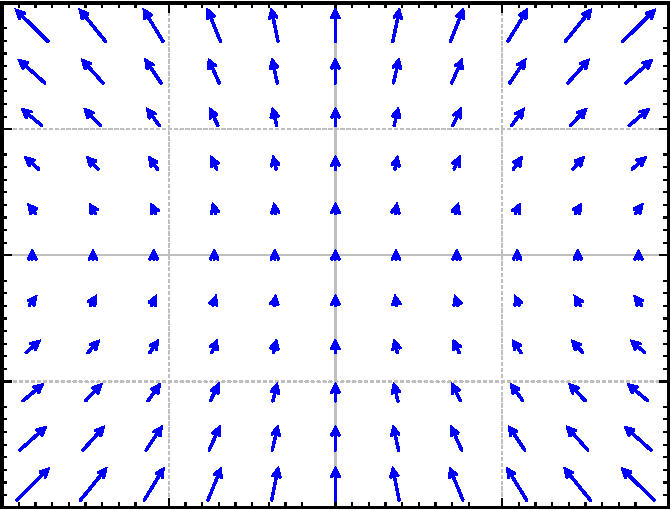
\includegraphics[width=1.75in]{figures/nlin-exer-xy-1py2}}
\task
\parbox[c]{1.75in}{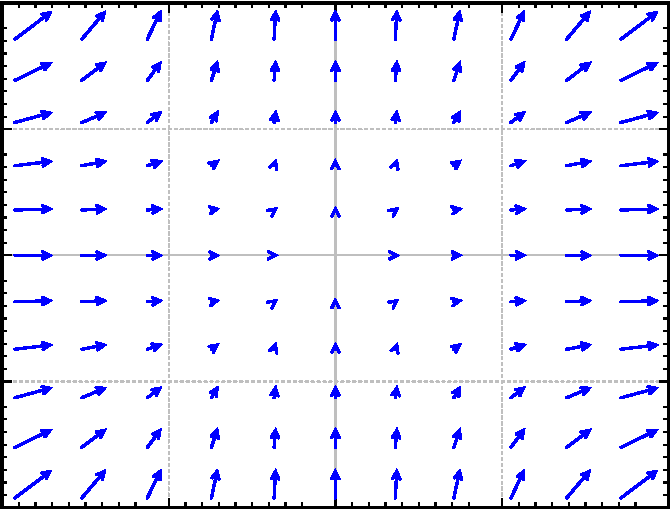
\includegraphics[width=1.75in]{figures/nlin-exer-x2-y2}}
\task
\parbox[c]{1.75in}{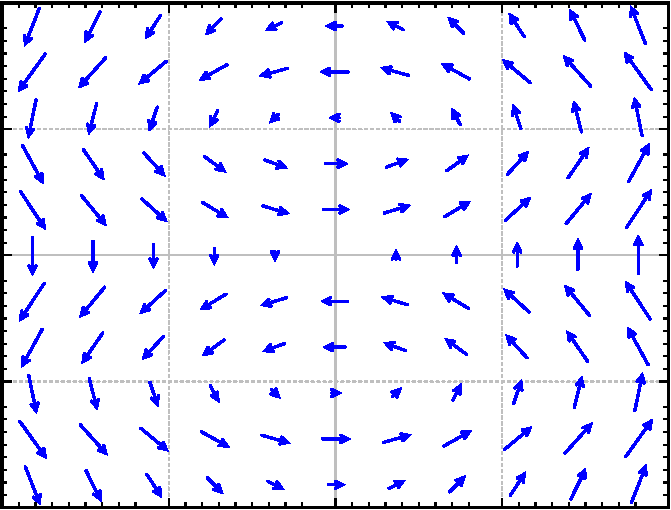
\includegraphics[width=1.75in]{figures/nlin-exer-sinpiy-x}}
\end{tasks}
\end{exercise}
\end{samepage}


\begin{exercise}
Find the critical points and linearizations of the following systems.
\begin{tasks}(2)
\task $x'=x^2-y^2$, \enspace $y'=x^2+y^2-1$,
\task $x'=-y$, \enspace $y'=3x+yx^2$,
\task $x'=x^2+y$, \enspace $y'=y^2+x$.
\end{tasks}
\end{exercise}

\begin{exercise}
For the following systems, verify they have critical point at $(0,0)$,
and find the linearization at $(0,0)$.
\begin{tasks}(2)
\task $x'=x+2y+x^2-y^2$, \enspace $y'=2y-x^2$
\task $x'=-y$, \enspace $y'=x-y^3$
\task* $x'=ax+by+f(x,y)$, $y'=cx+dy+g(x,y)$, where
$f(0,0) = 0$,
$g(0,0) = 0$, and all first partial derivatives of $f$ and $g$ are
also zero at $(0,0)$, that is,
$\frac{\partial f}{\partial x}(0,0) = 
\frac{\partial f}{\partial y}(0,0) = 
\frac{\partial g}{\partial x}(0,0) = 
\frac{\partial g}{\partial y}(0,0) = 0$.
\end{tasks}
\end{exercise}

\begin{exercise}
Take $x'=(x-y)^2$, \enspace $y'=(x+y)^2$. 
\begin{tasks}
\task Find the set of critical points.
\task Sketch a phase diagram and describe the behavior near the critical
point(s).
\task Find the linearization.  Is it helpful in understanding the system?
\end{tasks}
\end{exercise}

\begin{exercise}
Take $x'=x^2$, \enspace $y'=x^3$.
\begin{tasks}
\task Find the set of critical points.
\task Sketch a phase diagram and describe the behavior near the critical
point(s).
\task Find the linearization.  Is it helpful in understanding the system?
\end{tasks}
\end{exercise}

\setcounter{exercise}{100}

\pagebreak[2]
\begin{exercise}
Find the critical points and linearizations of the following systems.
\begin{tasks}(2)
\task $x'=\sin(\pi y)+(x-1)^2$, \enspace $y'=y^2-y$,
\task $x'=x+y+y^2$, \enspace $y'=x$,
\task $x'=(x-1)^2+y$, \enspace $y'=x^2+y$.
\end{tasks}
\end{exercise}
\exsol{%
a) Critical points $(0,0)$ and $(0,1)$.  At $(0,0)$ using $u=x$, $v=y$ the linearization is $u'=-2u-(\nicefrac{1}{\pi})v$, $v'=-v$.
At $(0,1)$ using $u=x$, $v=y-1$ the linearization is
$u'=-2u+(\nicefrac{1}{\pi})v$, $v'=v$.\\
b) Critical point $(0,0)$.  Using $u=x$, $v=y$ the linearization is
$u'=u+v$, $v'=u$.\\
c) Critical point $(\nicefrac{1}{2},\nicefrac{-1}{4})$.  Using
$u=x-\nicefrac{1}{2}$, $v=y+\nicefrac{1}{4}$ the linearization is
$u'=-u+v$, $v'=u+v$.
}

\begin{exercise}
Match systems
\begin{tasks}[counter-format=tsk[1])](2)
\task $x'=y^2$, \enspace $y'=-x^2$,
\task $x'=y$, \enspace $y'=(x-1)(x+1)$,
\task $x'=y+x^2$, \enspace $y'=-x$,
\end{tasks}
to the vector fields below.  Justify.
\begin{tasks}(3)
\task
\parbox[c]{1.75in}{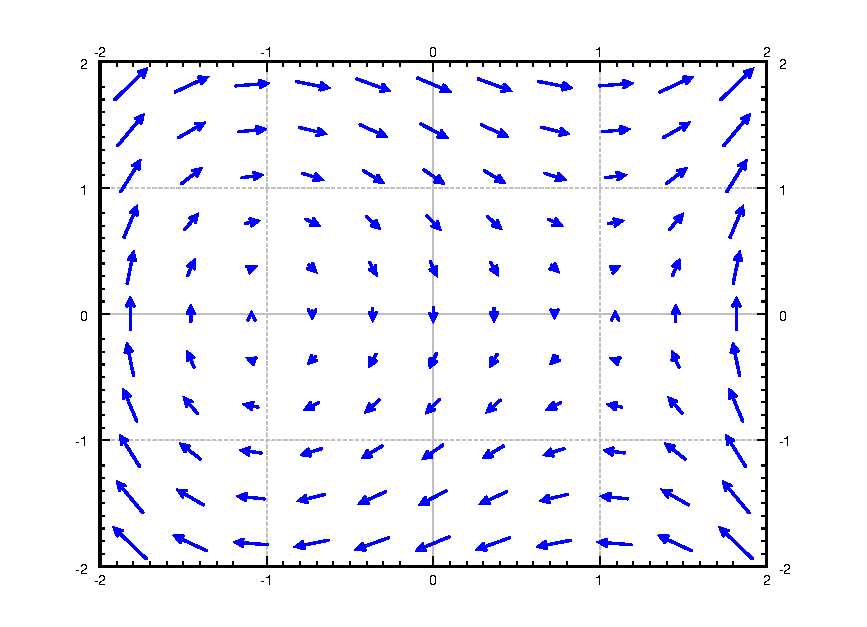
\includegraphics[width=1.75in]{figures/nlin-exer-y-xm1xp1}}
\task
\parbox[c]{1.75in}{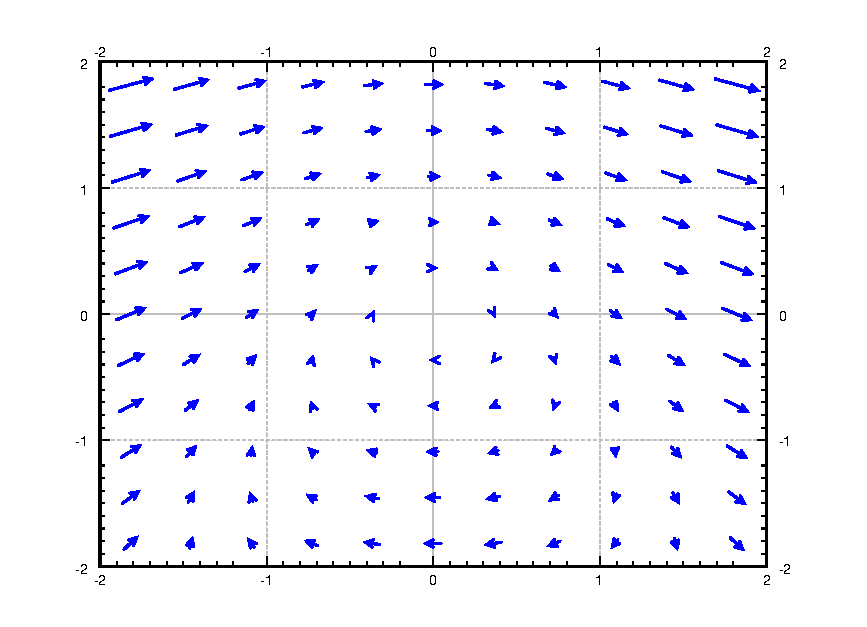
\includegraphics[width=1.75in]{figures/nlin-exer-ypx2-mx}}
\task
\parbox[c]{1.75in}{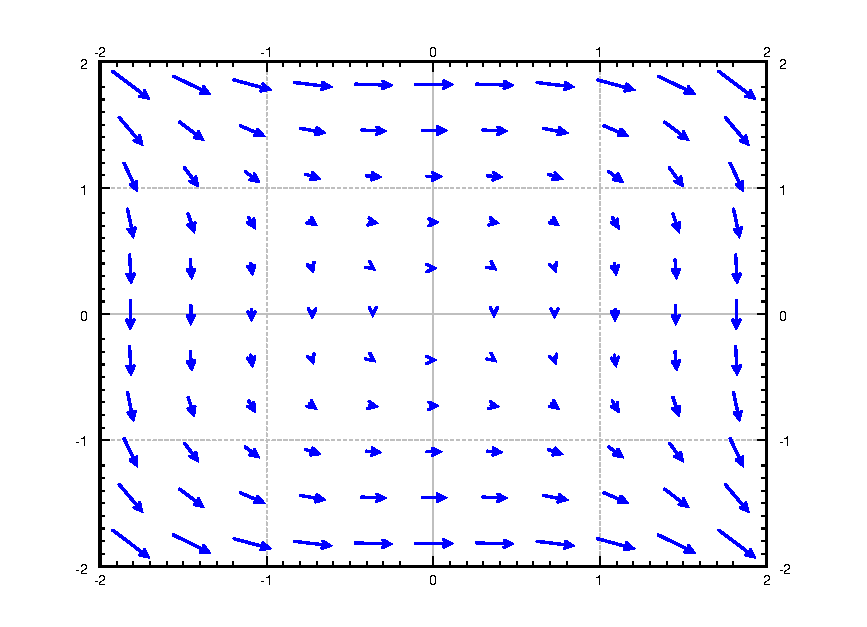
\includegraphics[width=1.75in]{figures/nlin-exer-y2-mx2}}
\end{tasks}
\end{exercise}
\exsol{%
1) is c), 2) is a), 3) is b)
}


\begin{samepage}
\begin{exercise}
The idea of critical points and linearization works in higher dimensions as
well.  You simply make the Jacobian matrix bigger by adding more functions
and more variables.  For the following system
of 3 equations find the critical points and their linearizations:
\begin{equation*}
x' = x + z^2, \qquad y' = z^2-y, \qquad z' = z+x^2.
\end{equation*}
\end{exercise}
\end{samepage}
\exsol{%
Critical points are $(0,0,0)$, and
$(-1, 1, -1)$.
The linearization at the origin using variables $u=x$, $v=y$, $w=z$ is
$u' = u$, $v'=-v$, $z' = w$.
The linearization at the point $(-1,1,-1)$ using variables $u=x+1$,
$v=y-1$, $w=z+1$ is
%$x=u-1$
%$y=v+1$
%$z=w-1$
%$u' = u-1 + (w-1)^2$, $v' = (w-1)^2-v+1$, $w' = (w-1)+(u-1)^2$.
%$u' = u + w^2-2w$, $v' = w^2-2w-v$, $w' = w+u^2-2u$
$u'=u-2w$, $v'=-v-2w$, $w'=w-2u$.
}

\begin{exercise}
Any two-dimensional non-autonomous system $x'=f(x,y,t)$, $y'=g(x,y,t)$ can
be written as a three-dimensional autonomous system (three equations).  Write down this
autonomous system using the variables $u$, $v$, $w$.
\end{exercise}
\exsol{%
$u' = f(u,v,w)$, $v'=g(u,v,w)$, $w' = 1$.
}

%%%%%%%%%%%%%%%%%%%%%%%%%%%%%%%%%%%%%%%%%%%%%%%%%%%%%%%%%%%%%%%%%%%%%%%%%%%%%%

\sectionnewpage
\section{Stability and classification of isolated critical points}
\label{nlinstability:section}

\sectionnotes{1.5--2 lectures\EPref{, \S6.1--\S6.2 in \cite{EP}}\BDref{,
\S9.2--\S9.3 in \cite{BD}}}

\subsection{Isolated critical points and almost linear systems}

A critical point is
\emph{isolated}\index{isolated critical point}
if it is the only critical point in some small
\myquote{neighborhood} of the point.  That is, if we zoom in far enough it is the
only critical point we see.  In the above example, the critical point was
isolated.  If on the other hand there would be a whole curve of critical
points, then it would not be isolated.

A system is called \emph{\myindex{almost linear}} at a critical point
$(x_0,y_0)$, if the critical point is isolated and the Jacobian matrix at the point
is invertible, or equivalently if the linearized system has an isolated
critical point.  In such a case, the nonlinear terms are very small
and the system behaves like its linearization, at least if we are close
to the critical point.

For example, the system in
Examples~\ref{example:nlin-1b-example} and \ref{example:nlin-1b-examplelin}
has two isolated critical points $(0,0)$ and $(0,1)$, and
is almost linear at both critical points as 
the Jacobian matrices at both points,
$\left[ \begin{smallmatrix} 0 & 1 \\ -1 & 0 \end{smallmatrix} \right]$ and
$\left[ \begin{smallmatrix} 0 & 1 \\ 1 & 0 \end{smallmatrix} \right]$,
are invertible.

On the other hand, the system $x' = x^2$, $y' = y^2$ has an isolated
critical point at $(0,0)$, however the Jacobian matrix
\begin{equation*}
\begin{bmatrix} 2x & 0 \\ 0 & 2y \end{bmatrix}
\end{equation*}
is zero when $(x,y) = (0,0)$.  So the system is not almost
linear.
Even a worse example is the system $x' = x$, $y' = x^2$, which does not have 
isolated critical points; $x'$ and $y'$ are both zero
whenever $x=0$, that is, the entire $y$ axis.

Fortunately, most often critical
points are isolated, and the system is almost linear at the critical
points.  So if we learn what happens there, we will have figured out the majority
of situations that arise in applications.



\subsection{Stability and classification of isolated critical points}

Once we have an isolated critical point, the system is almost linear at
that critical point, and we computed the
associated linearized system, we can classify what happens to the 
solutions.  We more or less use the classification for linear
two-variable systems from \sectionref{sec:twodimaut}, with one minor
caveat.
Let us list the behaviors depending on the eigenvalues of
the Jacobian matrix at the critical point in \tablevref{pln:behtab2}.
This table is very similar to \tablevref{pln:behtab}, with
the exception of missing \myquote{center} points.
%There is also a new column
%that we will discuss.
We will discuss centers later, as they are more complicated.

\begin{table}[h!t]
\mybeginframe
\capstart
\begin{center}
\begin{tabular}{@{}lll@{}}
\toprule
Eigenvalues of the Jacobian matrix & Behavior & Stability \\
\midrule
real and both positive & source / unstable node & unstable \\
real and both negative & sink / stable node & asymptotically stable \\
real and opposite signs & saddle & unstable \\
complex with positive real part & spiral source & unstable \\
complex with negative real part & spiral sink & asymptotically stable \\
\bottomrule
\end{tabular}
\end{center}
\caption{Behavior of an almost linear system near an isolated critical
point.  \label{pln:behtab2}}
\myendframe
\end{table}

In the third column,
we mark points as \emph{asymptotically stable} or \emph{unstable}.  Formally, a
\emph{\myindex{stable critical point}} $(x_0,y_0)$ is one where given any small distance $\epsilon$ to
$(x_0,y_0)$, and any initial condition within a perhaps smaller radius
around $(x_0,y_0)$, the trajectory
of the system never goes further away from $(x_0,y_0)$ than $\epsilon$.
An \emph{\myindex{unstable critical point}} is one that is not stable.
Informally, a point is stable if we start close to a critical point and
follow a trajectory we either go towards, or at least not away
from,
this critical point.

A stable critical point $(x_0,y_0)$ is called \emph{\myindex{asymptotically stable}} if
given any initial condition sufficiently close to $(x_0,y_0)$ and any
solution $\bigl( x(t), y(t) \bigr)$ satisfying that condition, then
\begin{equation*}
\lim_{t \to \infty} \bigl( x(t), y(t) \bigr) = (x_0,y_0) .
\end{equation*}
That is, the critical point is asymptotically stable
if any trajectory for a sufficiently close initial condition
goes towards the critical point $(x_0,y_0)$.

\begin{example} \label{example:nlin-xplusy}
Consider
$x'=-y-x^2$,
$y'=-x+y^2$.
See \figurevref{fig:nlin-ex813-new} for the phase diagram.
Let us find the critical points.  These are the points where
$-y-x^2 = 0$ and $-x+y^2=0$.  The first equation means $y = -x^2$, and
so $y^2 = x^4$.  Plugging into the second equation we obtain 
$-x+x^4 = 0$.  Factoring we obtain $x(1-x^3)=0$.  Since we are looking only
for real solutions we get either $x=0$ or $x=1$.  Solving for the
corresponding $y$ using $y = -x^2$, we get two critical points, one being $(0,0)$
and the other being $(1,-1)$.  Clearly the critical points are isolated.

\begin{myfig}
\capstart
\diffyincludegraphics{width=3in}{width=4.5in}{nlin-ex813-new}
\caption{The phase portrait with few sample trajectories of 
$x'=-y-x^2$, $y'=-x+y^2$.  \label{fig:nlin-ex813-new}}
\end{myfig}


Let us compute the Jacobian matrix:
\begin{equation*}
\begin{bmatrix}
-2x & -1 \\
-1 & 2y
\end{bmatrix} .
\end{equation*}
At the point $(0,0)$ we get the matrix
$\left[ \begin{smallmatrix} 0 & -1 \\ -1 & 0 \end{smallmatrix} \right]$ and
so the two eigenvalues are $1$ and $-1$.  As the matrix is invertible, the system is almost linear
at $(0,0)$.  As the eigenvalues are real
and of opposite signs, we get a saddle point, which is an unstable
equilibrium point.

At the point $(1,-1)$ we get the matrix
$\left[ \begin{smallmatrix} -2 & -1 \\ -1 & -2 \end{smallmatrix} \right]$ and
computing the eigenvalues we get $-1$, $-3$.
The matrix is invertible, and so the system is almost linear at $(1,-1)$.
As we have real eigenvalues and both negative, the critical
point is a sink, and therefore an asymptotically stable equilibrium point.
That is, if we start with any point $(x_i,y_i)$ close to $(1,-1)$ as
an initial condition and plot a trajectory, it approaches $(1,-1)$.
In other words,
\begin{equation*}
\lim_{t \to \infty} \bigl( x(t), y(t) \bigr) = (1,-1) .
\end{equation*}
As you can 
see from the diagram, this behavior is true even for some
initial points quite far from $(1,-1)$, but it is definitely not true for all
initial points.
\end{example}

\begin{example} \label{example:nlin-withexp}
Let us look at
$x'=y+y^2e^x$,
$y'=x$.  First let us find the critical points.  These are the points where
$y+y^2e^x = 0$ and $x=0$.  Simplifying we get $0=y+y^2 = y(y+1)$.  So the
critical points are $(0,0)$ and $(0,-1)$, and hence are isolated.  Let us
compute the Jacobian matrix:
\begin{equation*}
\begin{bmatrix}
y^2e^x & 1+2ye^x \\
1 & 0
\end{bmatrix}.
\end{equation*}

At the point $(0,0)$ we get the matrix
$\left[ \begin{smallmatrix} 0 & 1 \\ 1 & 0 \end{smallmatrix} \right]$ and
so the two eigenvalues are $1$ and $-1$.  As the matrix is invertible, the system is almost linear
at $(0,0)$.  And, as the eigenvalues are real
and of opposite signs, we get a saddle point, which is an unstable
equilibrium point.

At the point $(0,-1)$ we get the matrix
$\left[ \begin{smallmatrix} 1 & -1 \\ 1 & 0 \end{smallmatrix} \right]$ whose
eigenvalues are $\frac{1}{2} \pm i \frac{\sqrt{3}}{2}$.
The matrix is invertible, and so the system is almost linear at $(0,-1)$.
As we have complex eigenvalues with positive real part, the critical
point is a spiral source, and therefore an unstable equilibrium point.

\begin{myfig}
\capstart
\diffyincludegraphics{width=3in}{width=4.5in}{nlin-ex813}
\caption{The phase portrait with few sample trajectories of 
$x'=y+y^2e^x$, $y'=x$.  \label{fig:nlin-ex813}}
\end{myfig}

See \figurevref{fig:nlin-ex813} for the phase diagram.  Notice the two
critical points, and the behavior of the arrows in the vector field around
these points.
\end{example}

\subsection{The trouble with centers}

Recall, a linear system with a center means that trajectories
travel in closed elliptical orbits
in some direction around the critical point.  Such
a critical point we call a \emph{\myindex{center}} or
a \emph{\myindex{stable center}}.  It is not an asymptotically 
stable critical point, as the trajectories never approach the critical
point, but at least if you start sufficiently close to the critical point,
you stay close to the critical point.  The simplest example of such
behavior is the linear system with a center.  Another
example is the critical point $(0,0)$ in
\examplevref{example:nlin-1b-example}.

The trouble with a center in a nonlinear system is that whether the
trajectory goes towards or away from the critical point is governed by the
sign of the real part of the eigenvalues of the Jacobian matrix, and the Jacobian
matrix
in a nonlinear system changes from point to point.  Since this real
part is zero at the critical point itself, it can have either sign nearby,
meaning the trajectory could be pulled towards or away from the critical
point.

\begin{example}
An example of such a problematic behavior is the system
$x'=y, y' = -x+y^3$.  The only critical point
is the origin $(0,0)$.  The Jacobian matrix is 
\begin{equation*}
\begin{bmatrix}
0 & 1 \\
-1 & 3 y^2 \\
\end{bmatrix} .
\end{equation*}
At 
$(0,0)$ the Jacobian matrix is
$\left[ \begin{smallmatrix}
0 & 1 \\
-1 & 0 \\
\end{smallmatrix} \right]$, which has eigenvalues $\pm i$.  So the
linearization has a center.

Using the quadratic equation, the eigenvalues of the
Jacobian matrix at any point $(x,y)$ are
\begin{equation*}
\lambda = 
\frac{3}{2}y^2 \pm
i
\frac{\sqrt{4-9y^4}}{2} .
\end{equation*}
At any point where $y \not= 0$ (so at most points near the origin), the eigenvalues have a positive real part ($y^2$ can
never be negative).  This positive real part 
pulls the trajectory away from the origin.  A sample trajectory for an
initial condition near the origin is given in
\figurevref{fig:nlin-unstable-center}.
\begin{myfig}
\capstart
\diffyincludegraphics{width=3in}{width=4.5in}{nlin-unstable-centerfig}
\caption{An unstable critical point (spiral source) at the origin
for $x'=y, y' = -x+y^3$, even if the linearization has a center.  \label{fig:nlin-unstable-center}}
\end{myfig}
\end{example}

The moral of the example is that further analysis is needed when the
linearization has a center.  The analysis will in general be more
complicated than in the above example, and is more likely to involve
case-by-case consideration.  Such a complication should not be
surprising to you.  By now in your mathematical career, you have
seen many places where a simple test is inconclusive, recall for example
the second derivative test for maxima or minima, and requires more careful,
and perhaps ad hoc analysis of the situation.

\subsection{Conservative equations}

An equation of the form
\begin{equation*}
x'' + f(x) = 0
\end{equation*}
for an arbitrary function $f(x)$ is called a
\emph{\myindex{conservative equation}}.  For example the pendulum equation
is a conservative equation.  The equations are conservative as there is no
friction in the system so the energy in the system is \myquote{conserved.}
Let us write this equation as a
system of nonlinear ODE.
\begin{equation*}
x' = y, \qquad y' = -f(x) .
\end{equation*}
These types of equations have the
advantage that we can solve for their trajectories easily.

The trick is to first think of $y$ as a function of $x$ for a moment.  Then
use the chain rule
\begin{equation*}
x'' = y' = \frac{dy}{dx} x' = y \frac{dy}{dx} ,
\end{equation*}
where the prime indicates a derivative with respect to $t$.  
We obtain $y \frac{dy}{dx} + f(x) = 0$.  We integrate with respect to
$x$ to get
$\int y \frac{dy}{dx} \,dx + \int f(x)\, dx = C$.  In other words
\begin{equation*}
\frac{1}{2} y^2  + \int f(x)\, dx = C .
\end{equation*}
We obtained an implicit equation for the trajectories, with different $C$
giving different trajectories.  The value of
$C$ is conserved on any trajectory.  This expression is
sometimes called the \emph{\myindex{Hamiltonian}} or the energy of the
system.
If you look back to \sectionref{exact:section}, you will notice
that $y\frac{dy}{dx} + f(x) = 0$ is an exact equation, and
we just found a potential function.

\begin{example}
Let us find the trajectories for the equation $x'' + x-x^2 = 0$,
which is the equation from
\examplevref{example:nlin-1b-example}.  The corresponding
first order system is
\begin{equation*}
x' = y , \qquad y' = -x+x^2 .
\end{equation*}
Trajectories satisfy
\begin{equation*}
\frac{1}{2} y^2  + \frac{1}{2} x^2 - \frac{1}{3} x^3  = C .
\end{equation*}
We solve for $y$
\begin{equation*}
y = \pm \sqrt{-x^2 + \frac{2}{3} x^3  + 2C} .
\end{equation*}

Plotting these graphs we get exactly the trajectories in 
\figurevref{fig:nlin-1b}.  In particular we notice that near the origin
the trajectories are \emph{\myindex{closed curves}}: they keep going
around the origin, never spiraling in or out.  Therefore we discovered a way
to verify that the critical point at $(0,0)$ is a stable center.
The critical point at $(0,1)$ is a saddle as we already noticed.
This example is typical for conservative equations.
\end{example}

Consider an arbitrary
conservative equation $x'' + f(x) = 0$.
All critical points occur when $y=0$ (the
$x$-axis), that is when $x' = 0$.  The critical points are 
those points on the $x$-axis where $f(x) = 0$.
The trajectories are given by
\begin{equation*}
y = \pm \sqrt{ - 2 \int f(x)\, dx + 2C} .
\end{equation*}
So all trajectories are mirrored across the $x$-axis.  In particular,
there can be no spiral sources nor sinks.
The Jacobian matrix is
\begin{equation*}
\begin{bmatrix}
0 & 1 \\
-f'(x) & 0
\end{bmatrix} .
\end{equation*}
The critical point is almost linear if $f'(x) \not= 0$ at the critical 
point.  Let $J$ denote the Jacobian matrix.
The eigenvalues of $J$ are solutions to
\begin{equation*}
0 = \det(J - \lambda I) = \lambda^2 + f'(x) .
\end{equation*}
Therefore $\lambda = \pm \sqrt{-f'(x)}$.  In other words, either we get
real eigenvalues of opposite signs (if $f'(x) < 0$),
or we get purely imaginary eigenvalues (if $f'(x) > 0$).
There are only two possibilities for critical points, either an \emph{unstable
saddle point}, or a \emph{stable center}.
There are never any sinks or sources.

\subsection{Exercises}

\begin{exercise}
For the systems below, find and classify the critical points, also indicate
if the equilibria are stable, asymptotically stable, or unstable.
\begin{tasks}(2)
\task $x'=-x+3x^2, y'=-y$
\task $x'=x^2+y^2-1$, $y'=x$
\task $x'=ye^x$, $y'=y-x+y^2$
\end{tasks}
\end{exercise}

\begin{exercise}
Find the implicit equations of the trajectories of the following
conservative systems.  Next find their critical points (if any) and classify them.
\begin{tasks}(2)
\task $x''+ x+x^3 = 0$
\task $\theta''+\sin \theta = 0$
\task $z''+ (z-1)(z+1) = 0$
\task $x''+ x^2+1 = 0$
\end{tasks}
\end{exercise}

\begin{exercise}
Find and classify the critical point(s) of $x' = -x^2$, $y' = -y^2$.
\end{exercise}

\begin{samepage}
\begin{exercise}
Suppose $x'=-xy$, $y'=x^2-1-y$.
\begin{tasks}
\task
Show there are two spiral sinks at
$(-1,0)$ and $(1,0)$.
\task
For any initial point of the form $(0,y_0)$, find what is the trajectory.
\task
Can a trajectory starting at $(x_0,y_0)$ where $x_0 > 0$ spiral into 
the critical point at $(-1,0)$?  Why or why not?
\end{tasks}
\end{exercise}
\end{samepage}

\begin{exercise} \label{exercise:increasing}
In the example $x'=y$, $y'=y^3-x$ show that for any trajectory, the distance
from the origin is an increasing function.
Conclude
that the origin behaves like is a spiral source.
Hint: Consider $f(t) =
{\bigl(x(t)\bigr)}^2 + 
{\bigl(y(t)\bigr)}^2$ and show it has positive derivative.
\end{exercise}


\begin{exercise}
Suppose $f$ is always positive.
Find the trajectories of $x''+f(x') = 0$.
Are there any critical points?
\end{exercise}

\begin{exercise}
Suppose that $x' = f(x,y)$, $y' = g(x,y)$.  Suppose that $g(x,y) > 1$ for
all $x$ and $y$.  Are there any critical points?  What can we say about the
trajectories at $t$ goes to infinity?
\end{exercise}

\setcounter{exercise}{100}

\begin{exercise}
For the systems below, find and classify the critical points.
\begin{tasks}(3)
\task $x'=-x+x^2$, $y'=y$
\task $x'=y-y^2-x$, $y'=-x$
\task $x'=xy$, $y'=x+y-1$
\end{tasks}
\end{exercise}
\exsol{%
a) $(0,0)$: saddle (unstable), $(1,0)$: source (unstable), \qquad
b) $(0,0)$: spiral sink (asymptotically stable), $(0,1)$: saddle (unstable), \qquad
c) $(1,0)$: saddle (unstable), $(0,1)$: saddle (unstable)
}

\begin{exercise}
Find the implicit equations of the trajectories of the following
conservative systems.  Next find their critical points (if any) and classify them.
\begin{tasks}(3)
\task $x''+ x^2 = 4$
\task $x''+ e^x = 0$
\task $x''+ (x+1)e^x = 0$
\end{tasks}
\end{exercise}
\exsol{%
a) $\frac{1}{2}y^2 + \frac{1}{3}x^3 -4x = C$, critical points
$(-2,0)$: an unstable saddle, and $(2,0)$: a stable center.
b) $\frac{1}{2}y^2 + e^x = C$, no critical points.
c) $\frac{1}{2}y^2 + xe^x = C$, critical point at $(-1,0)$ is a stable center.
}

\begin{exercise}
The conservative system $x''+x^3 = 0$ is not almost linear.  Classify
its critical point(s) nonetheless.
\end{exercise}
\exsol{%
Critical point at $(0,0)$.
Trajectories are $y = \pm \sqrt{2C+(\nicefrac{1}{2})x^4}$, for $C > 0$, these give closed
curves around the origin, so the critical point is a stable center.
}

\begin{exercise}
Derive an analogous classification of critical points for equations in one dimension,
such as $x'= f(x)$ based on the derivative.  A point $x_0$ is critical when $f(x_0) = 0$ and
almost linear if in addition $f'(x_0) \not= 0$.  Figure out if the critical point is stable or unstable
depending on the sign of $f'(x_0)$.  Explain.  Hint: see \sectionref{auteq:section}.
\end{exercise}
\exsol{%
A critical point $x_0$ is stable if $f'(x_0) < 0$ and unstable when $f'(x_0)
> 0$.
}

%%%%%%%%%%%%%%%%%%%%%%%%%%%%%%%%%%%%%%%%%%%%%%%%%%%%%%%%%%%%%%%%%%%%%%%%%%%%%%

\sectionnewpage
\section{Applications of nonlinear systems}
\label{nlinapps:section}

\sectionnotes{2 lectures\EPref{, \S6.3--\S6.4 in \cite{EP}}\BDref{, \S9.3,
\S9.5 in \cite{BD}}}

In this section we study two very standard examples of nonlinear
systems.  First, we look at the nonlinear pendulum equation.  We saw
the pendulum equation's linearization before, but we noted it
was only valid for small angles and short times.  Now we find out what
happens for large angles.  Next, we look at the predator-prey equation,
which finds various applications in modeling problems in biology, chemistry,
economics, and elsewhere.

\subsection{Pendulum}

The first example we study is the pendulum equation
$\theta''+\frac{g}{L} \sin \theta = 0$.  Here, $\theta$ is the angular
displacement, $g$ is the gravitational constant, and $L$ is the length of
the pendulum.  In this equation we disregard friction, so we are talking
about an idealized pendulum.

\begin{mywrapfigsimp}{1.45in}{1.75in}
\noindent
\inputpdft{mv-pend}
\end{mywrapfigsimp}
This equation is a conservative
equation, so we can use our analysis of conservative equations
from the previous section.
Let us change the equation to a two-dimensional
system in variables $(\theta,\omega)$ by introducing the new
variable $\omega$:
\begin{equation*}
\begin{bmatrix}
\theta \\ \omega
\end{bmatrix} '
=
\begin{bmatrix}
\omega \\
- \frac{g}{L} \sin \theta
\end{bmatrix} .
\end{equation*}
The critical points of this system are when $\omega = 0$ and $-\frac{g}{L}
\sin \theta = 0$, or in other words if $\sin \theta = 0$.  So the critical
points are when $\omega = 0$ and $\theta$ is a multiple of $\pi$.  That is,
the points are $\ldots (-2\pi,0), (-\pi,0), (0,0), (\pi,0), (2\pi,0)
\ldots$.  While there are infinitely many critical points, they are all isolated.
Let us compute the Jacobian matrix:
\begin{equation*}
\begin{bmatrix}
\frac{\partial}{\partial \theta} \Bigl( \omega \Bigr) & 
\frac{\partial}{\partial \omega} \Bigl( \omega \Bigr) \\
\frac{\partial}{\partial \theta} \Bigl( - \frac{g}{L} \sin \theta \Bigr) & 
\frac{\partial}{\partial \omega} \Bigl( - \frac{g}{L} \sin \theta \Bigr)
\end{bmatrix}
=
\begin{bmatrix}
0 & 1 \\
- \frac{g}{L} \cos \theta & 0
\end{bmatrix} .
\end{equation*}

For conservative equations, there are two types of
critical points.  Either stable centers, or saddle points.  The eigenvalues
of the Jacobian matrix are $\lambda = \pm \sqrt{-\frac{g}{L}\cos \theta}$.

The
eigenvalues are going to be real when $\cos \theta < 0$.  This happens at the odd multiples of $\pi$.
The
eigenvalues are going to be purely imaginary 
when $\cos \theta > 0$.  This happens at the even
multiples of $\pi$.  Therefore the system has a stable center at
the points $\ldots (-2\pi,0), (0,0), (2\pi,0) \ldots$, and it has an
unstable saddle at
the points $\ldots (-3\pi,0), (-\pi,0), (\pi,0), (3\pi,0) \ldots$.  Look at the
phase diagram in \figurevref{fig:nlin-pend-phasediag},
where for simplicity we let $\frac{g}{L} = 1$.

\begin{myfig}
\capstart
\diffyincludegraphics{width=3in}{width=4.5in}{nlin-pend-phasediag}
\caption{Phase plane diagram and some trajectories of
the nonlinear pendulum equation. \label{fig:nlin-pend-phasediag}}
\end{myfig}

In the linearized equation we have only a single critical point, the center
at $(0,0)$.  Now we see more clearly what we meant when we said the
linearization is good for small angles.  The horizontal axis is the
deflection angle.  The vertical axis is the angular velocity of the
pendulum.  Suppose we start at $\theta = 0$ (no deflection), and
we start with a small angular velocity $\omega$.  Then the trajectory keeps going
around the critical point $(0,0)$ in an approximate circle.  This
corresponds to short swings of the pendulum back and forth.  When $\theta$
stays small, the trajectories really look like circles and hence are very
close to our linearization.

When we give the pendulum a big enough push, it
goes across the top and keeps spinning about its axis.  This behavior
corresponds to the
wavy curves that do not cross the horizontal axis in the phase diagram.
Let us suppose we look at the top curves, when the angular velocity $\omega$
is large and positive.  Then the pendulum is going
around and around its axis.  The velocity is going to
be large when the pendulum is near the bottom, and the velocity is the
smallest when the pendulum
is close to the top of its loop.

At each critical point, there is an equilibrium solution.  Consider
the solution
$\theta = 0$;  the pendulum is not moving
and is hanging straight down.  This is a stable place for the
pendulum to be, hence this is a \emph{stable} equilibrium.

The other type of equilibrium solution is at the unstable point, for example
$\theta = \pi$.  Here the pendulum is upside down.  Sure you can balance the
pendulum this way and it will stay, but this is an \emph{unstable} equilibrium.
Even the tiniest push will make the pendulum start swinging wildly.

See \figurevref{fig:nlin-pend} for a diagram.  The first picture is the
stable equilibrium $\theta = 0$.  The second picture corresponds to those
\myquote{almost circles} in the phase diagram around $\theta =0$ when the angular
velocity is small.  The next picture is the unstable equilibrium $\theta =
\pi$.  The last picture corresponds to the wavy lines for large angular
velocities.

\begin{myfig}
\capstart
\inputpdft{nlin-pend}
\caption{Various possibilities for the motion of the pendulum. \label{fig:nlin-pend}}
\end{myfig}

The quantity 
\begin{equation*}
\frac{1}{2} \omega^2  - \frac{g}{L} \cos \theta 
\end{equation*}
is conserved by any solution.  This is the energy or the Hamiltonian of
the system.

We have a conservative equation and so (exercise) the
trajectories are given by
\begin{equation*}
\omega = \pm \sqrt{ \frac{2g}{L} \cos \theta + C} ,
\end{equation*}
for various values of $C$.  
Let us look at the initial condition of $(\theta_0,0)$,
that is, we take the pendulum to
angle $\theta_0$, and just let it go (initial angular velocity 0).
We plug the initial conditions into the above and solve for $C$ to obtain
\begin{equation*}
C = - \frac{2g}{L} \cos \theta_0 .
\end{equation*}
Thus the expression for the trajectory is
\begin{equation*}
\omega = \pm \sqrt{ \frac{2g}{L}} \sqrt{ \cos \theta - \cos \theta_0 } .
\end{equation*}

Let us figure out the period.  That is, the time it takes for the pendulum
to swing back and forth.
We notice that the trajectory about the
origin in the phase plane is symmetric about both the $\theta$ and the
$\omega$ axis.  That is, in terms of $\theta$,
the time it takes from $\theta_0$ to $-\theta_0$
is the same as it takes from $-\theta_0$ back to $\theta_0$.  Furthermore,
the time it takes from $-\theta_0$ to $0$ is the same as to go from $0$ to
$\theta_0$.  Therefore, let us find how long it takes for
the pendulum to go from angle 0 to angle $\theta_0$, which is a quarter of
the full oscillation and then multiply by 4.

We figure out this time by finding
$\frac{dt}{d\theta}$ and integrating from $0$ to $\theta_0$.
The period is four times
this integral.  Let us stay in the region where $\omega$ is positive.
Since $\omega = \frac{d\theta}{dt}$, inverting we get
\begin{equation*}
\frac{dt}{d\theta} = \sqrt{\frac{L}{2g}} \frac{1}{\sqrt{\cos \theta - \cos \theta_0 }} .
\end{equation*}
Therefore the period $T$ is given by
\begin{equation*}
T = 4 \sqrt{\frac{L}{2g}} \int_0^{\theta_0} \frac{1}{\sqrt{\cos \theta -
\cos \theta_0 }}\, d\theta .
\end{equation*}
The integral is an improper integral, and we cannot in
general evaluate it symbolically.  We must resort to numerical
approximation if we want to compute a particular $T$.

Recall from \sectionref{sec:mv}, the linearized equation $\theta''+\frac{g}{L}\theta
= 0$ has period
\begin{equation*}
T_{\text{linear}} = 2\pi \sqrt{\frac{L}{g}} .
\end{equation*}
We plot $T$, $T_{\text{linear}}$, and the relative error
$\frac{T-T_{\text{linear}}}{T}$ in \figurevref{fig:TvsT0}.  The relative error
says how far is our approximation from the real period percentage-wise.
Note that $T_{\text{linear}}$ is simply a constant, it does not change with
the initial angle $\theta_0$.  The actual period $T$ gets larger and larger as
$\theta_0$ gets larger.
Notice how the relative error is small when $\theta_0$ is small.  It is
still only $15\%$ when $\theta_0 = \frac{\pi}{2}$, that is, a 90 degree
angle.  The error is $3.8\%$ when starting at $\frac{\pi}{4}$, 
a 45 degree angle.  At a 5 degree initial angle, the error is only $0.048 \%$.

\begin{myfig}
\capstart
%original files nlin-T-vs-T0-abs nlin-T-vs-T0-relerr
\diffyincludegraphics{width=6.24in}{width=9in}{nlin-T-vs-T0-abs-relerr}
\caption{The plot of $T$ and $T_{\text{linear}}$ with $\frac{g}{L} =
1$ (left), and the plot of the relative
error $\frac{T-T_{\text{linear}}}{T}$ (right), for $\theta_0$ between 0 and $\pi/2$. \label{fig:TvsT0}}
\end{myfig}

While it is not immediately obvious from the formula, it is true that
\begin{equation*}
\lim_{\theta_0 \uparrow \pi} T = \infty .
\end{equation*}
That is, the period goes to infinity as the initial angle approaches the
unstable equilibrium point.  So if we put the pendulum almost upside down it
may take a very long time before it gets down.  This is consistent with the
limiting behavior, where the exactly upside down pendulum never makes an
oscillation, so we could think of that as infinite period.

\subsection{Predator-prey or Lotka--Volterra systems}

One of the most common simple applications of nonlinear systems are the
so-called \emph{\myindex{predator-prey}} or
\emph{\myindex{Lotka--Volterra}}%
\footnote{Named for the American mathematician, chemist, and statistician
\href{https://en.wikipedia.org/wiki/Alfred_J._Lotka}{Alfred James Lotka}
(1880--1949) and the Italian mathematician and physicist
\href{https://en.wikipedia.org/wiki/Vito_Volterra}{Vito Volterra}
(1860--1940).}
systems.  For example, these systems arise 
when two species interact, one as the prey and one as the predator.  It is
then no surprise that the equations also see applications in economics.
The system also arises in chemical reactions.
In biology, this system of equations explains the natural periodic variations of populations of
different species in nature.  Before the application of differential
equations, these periodic variations in the population baffled biologists.

We keep
with the classical example of hares and foxes in a forest, it is the
easiest to understand.
\begin{equation*}
\begin{aligned}
& x = \# \text{ of hares (the prey),} \\
& y = \# \text{ of foxes (the predator).}
\end{aligned}
\end{equation*}
When there are a lot of hares, there is plenty of food for the foxes, so
the fox population grows.  However, when the fox population grows, the foxes
eat more hares, so when there are lots of foxes, the hare population
should go down, and vice versa.
The Lotka--Volterra model proposes that this 
behavior is described by the system of equations
\begin{equation*}
\begin{aligned}
& x' = (a-by)x, \\
& y' = (cx-d)y,
\end{aligned}
\end{equation*}
where $a,b,c,d$ are some parameters that describe the interaction of the
foxes and hares\footnote{This interaction does not end well for the
hare.}.  In this model, these are all positive numbers.

Let us analyze the idea behind this model.  The model is a slightly more
complicated idea based on the exponential population model.
First expand,
\begin{equation*}
x' = (a-by)x = ax - byx .
\end{equation*}
The hares are expected to simply grow exponentially in the absence of foxes,
that is where the $ax$ term comes in, the growth in population is
proportional to the population itself.  We are assuming the hares
always find enough food and have enough space to reproduce.  However,
there is another component $-byx$, that is, the population also is
decreasing proportionally to the number of foxes.  Together we can write the
equation as $(a-by)x$, so it is like exponential growth or decay but the
constant depends on the number of foxes.

The equation for foxes is very similar, expand again
\begin{equation*}
y' = (cx-d)y = cxy-dy .
\end{equation*}
The foxes need food (hares) to reproduce: the more food, the bigger the
rate of growth, hence the $cxy$ term.  On the other hand, there are 
natural deaths in the fox population, and hence the $-dy$ term.

Without further delay, let us start with an explicit example.  Suppose the
equations are 
\begin{equation*}
x' = (0.4-0.01y)x, \qquad y' = (0.003x-0.3)y .
\end{equation*}
See \figurevref{fig:nlin-pred-prey} for the phase portrait.  In this example
it makes sense to also plot $x$ and $y$ as graphs with respect to time.
Therefore the second graph in 
\figureref{fig:nlin-pred-prey} is the graph of $x$ and $y$ on the vertical
axis (the prey $x$ is the thinner line with taller peaks), against time
on the horizontal axis.  The particular solution graphed was with initial
conditions of 20 foxes and 50 hares.
\begin{myfig}
\capstart
%original files nlin-pred-prey-phase nlin-pred-prey-graphs
\diffyincludegraphics{width=6.24in}{width=9in}{nlin-pred-prey-phase-graphs}
\caption{The phase portrait (left) and graphs of $x$ and $y$ for
a sample solution (right). \label{fig:nlin-pred-prey}}
\end{myfig}

Let us analyze what we see on the graphs.  We work in the general
setting rather than putting in specific numbers.  We start with finding
the critical points.  Set $(a-by)x = 0$, and $(cx-d)y = 0$.
The first equation is satisfied if either $x=0$ or $y=\nicefrac{a}{b}$.  If $x=0$, the
second equation implies $y=0$.  If $y= \nicefrac{a}{b}$, the second equation implies
$x=\nicefrac{d}{c}$.
There are two equilibria: at $(0,0)$ when there are no animals at all, and at
$(\nicefrac{d}{c},\nicefrac{a}{b})$.  
In our specific example $x = \nicefrac{d}{c} = 100$, and $y = \nicefrac{a}{b} = 40$.
This is the point where there are 100 hares and 40 foxes.

We compute the Jacobian matrix:
\begin{equation*}
\begin{bmatrix}
a-by & -bx \\
cy & cx-d
\end{bmatrix} .
\end{equation*}
At the origin $(0,0)$ we get the matrix
$\left[ \begin{smallmatrix}
a & 0 \\
0 & -d
\end{smallmatrix} \right]$, so the eigenvalues are $a$ and $-d$, hence real
and of opposite signs.  So the critical point at the origin is a saddle.
This makes sense.  If you started with some foxes but no hares, then the
foxes would go extinct, that is, you would approach the origin.  If you
started with no foxes and a few hares, then the hares would keep multiplying
without check, and so you would go away from the origin.

OK, how about the other critical point at $(\nicefrac{d}{c},\nicefrac{a}{b})$.  Here
the Jacobian matrix becomes
\begin{equation*}
\begin{bmatrix}
0 & -\frac{bd}{c} \\
\frac{ac}{b} & 0
\end{bmatrix} .
\end{equation*}
The eigenvalues satisfy $\lambda^2 + ad = 0$.  In
other words, $\lambda = \pm i \sqrt{ad}$.  The eigenvalues being
purely imaginary, we are in the case where we cannot quite decide using only
linearization.  We could
have a stable center, spiral sink, or a spiral source.  That is, the
equilibrium could be asymptotically stable, stable, or unstable.  Of
course I gave you a picture above that seems to imply it is a stable
center.  But never trust a picture only.  Perhaps the oscillations
are getting larger and larger, but only \emph{very} slowly.  Of course this would be
bad as it would imply something will go wrong with our population
sooner or later.  And I only graphed a very specific example with very
specific trajectories.

How can we be sure we are in the stable situation?
As we said before, in the case of purely imaginary eigenvalues, we have to
do a bit more work.  Previously we found that for conservative systems,
there was a certain quantity that was conserved on the trajectories, and
hence the trajectories had to go in closed loops.
We can use a similar technique here.  We just have to figure out what is the
conserved quantity.  After some trial and error we find the
constant
\begin{equation*}
C = \frac{y^a x^d}{e^{cx+by}} = y^a x^d e^{-cx-by}
\end{equation*}
is conserved.  Such a quantity is called the \emph{\myindex{constant of
motion}}.  Let us check $C$ really is a constant of motion.  How do we check, you say?  Well, a constant is
something that does not change with time, so let us compute the derivative
with respect to time:
\begin{equation*}
C' = 
a y^{a-1}y' x^d e^{-cx-by}
+
y^a d x^{d-1} x' e^{-cx-by}
+
y^a x^d e^{-cx-by} (-cx'-by') .
\end{equation*}
Our equations give us what $x'$ and $y'$ are so let us plug those in:
\begin{equation*}
\begin{split}
C' & = 
a y^{a-1} (cx-d)y x^d e^{-cx-by}
+
y^a d x^{d-1} (a-by)x e^{-cx-by}
\\
& \phantom{mm} +
y^a x^d e^{-cx-by} \bigl(-c(a-by)x-b(cx-d)y\bigr)
\\
& =
y^a x^d e^{-cx-by}
\Bigl(
a (cx-d)
+
d (a-by)
+
\bigl(-c(a-by)x-b(cx-d)y\bigr) \Bigr)
\\
& = 
0 .
\end{split}
\end{equation*}
So along the trajectories $C$ is constant.  In fact, the expression $C =
\frac{y^a x^d}{e^{cx+by}}$ gives us an implicit equation for the
trajectories.  In any case, once we have found this constant of motion,
it must be true that the
trajectories are simple curves, that is, the level curves of
$\frac{y^a x^d}{e^{cx+by}}$.  It turns out, the critical point at
$(\nicefrac{d}{c},\nicefrac{a}{b})$ is a maximum for $C$ (left as an exercise).
So $(\nicefrac{d}{c},\nicefrac{a}{b})$ is a stable equilibrium point, and 
we do not have to worry about the foxes and hares going extinct or their
populations exploding.

One blemish on this wonderful model is that the number of foxes and hares
are discrete quantities and we are modeling with continuous variables.  Our
model has no problem with there being 0.1 fox in the forest for example,
while in reality that makes no sense.  The approximation is a reasonable one
as long as the number of foxes and hares are large, but it does not make
much sense for small numbers.  One must be careful in interpreting any
results from such a model.

An interesting consequence (perhaps counterintuitive) of this model is that adding animals to
the forest might lead to extinction, because the variations will get too
big, and one of the populations will get close to zero.  For example, suppose there are 20 foxes and 50 hares as
before, but now we bring in more foxes, bringing their number to 200.  If we
run the computation, we find the number of hares will plummet to just
slightly more than 1 hare in the whole forest.  In reality that most
likely means the hares die out, and then the foxes will die out as well
as they will have nothing to eat.

Showing that a system of equations has a stable solution can be a very
difficult problem.  When Isaac Newton put forth his laws of
planetary motions, he proved that a single planet orbiting a single sun is a
stable system.  But any solar system with more than 1 planet proved very
difficult indeed.  In fact, such a system behaves chaotically (see 
\sectionref{sec:chaos}), meaning small changes in initial conditions lead to very
different long-term outcomes.  From numerical experimentation and
measurements, we know the earth will not fly out into the empty space
or crash into the sun, for at least some millions of years or so.
But we do not know what happens beyond that.

\subsection{Exercises}

\begin{exercise}
Take the \emph{\myindex{damped nonlinear pendulum equation}} $\theta '' + \mu \theta' +
(\nicefrac{g}{L})
\sin \theta = 0$ for some $\mu > 0$ (that is, there is some friction).
\begin{tasks}
\task
Suppose $\mu = 1$ and $\nicefrac{g}{L} = 1$ for simplicity, find and
classify the critical points.
\task
Do the same for any $\mu > 0$ and any $g$
and $L$, but such that the damping is small, in particular, $\mu^2 <
4(\nicefrac{g}{L})$.
\task
Explain what your findings mean, and if it agrees with what you
expect in reality.
\end{tasks}
\end{exercise}

\begin{exercise}
Suppose the hares do not grow exponentially, but logistically.  In
particular consider
\begin{equation*}
x' = (0.4-0.01y)x - \gamma x^2, \qquad y' = (0.003x-0.3)y .
\end{equation*}
For the following two values of $\gamma$,
find and classify all the critical points in the positive quadrant, that is, for
$x \geq 0$ and $y \geq 0$.  Then sketch the phase diagram.  Discuss the
implication for the long term behavior of the population.
\begin{tasks}(2)
\task
$\gamma=0.001$, 
\task
$\gamma=0.01$.
\end{tasks}
\end{exercise}

\begin{exercise}
{\ }
\begin{tasks}
\task Suppose $x$ and $y$ are
positive variables.  Show $\frac{y x}{e^{x+y}}$
attains a maximum at $(1,1)$.
\task Suppose $a,b,c,d$ are positive constants, and also suppose $x$ and $y$ are
positive variables.  Show $\frac{y^a x^d}{e^{cx+by}}$
attains a maximum at $(\nicefrac{d}{c},\nicefrac{a}{b})$.
\end{tasks}
\end{exercise}

\begin{exercise}
Suppose that for the pendulum equation we take a trajectory giving the
spinning-around motion, for example $\omega = \sqrt{\frac{2g}{L} \cos \theta
+ \frac{2g}{L} + \omega_0^2}$.  This is the trajectory where the lowest
angular velocity is $\omega_0^2$.  Find an integral expression for how long it takes
the pendulum to go all the way around.
\end{exercise}

%Suppose we have the system predator-prey system where the foxes are also
%hunted at a constant rate $hy$ proportional to the population.  That is,
%$x' = (a-by)x,$  $y' = (cx-d)y - hy$.  Find and analyze the critical points.

\begin{exercise}[challenging]
Take the pendulum, suppose the initial position is $\theta = 0$.
\begin{tasks}
\task
Find the expression for $\omega$ giving the trajectory
with initial condition $(0,\omega_0)$.  Hint: Figure out what $C$
should be in terms of $\omega_0$.
\task
Find the crucial angular velocity $\omega_1$, such that
for any higher initial angular velocity,
the pendulum will keep going around its
axis, and for any lower initial angular velocity, the pendulum will simply
swing back and forth.
Hint: When the pendulum doesn't go over the top the expression for $\omega$
will be undefined for some $\theta$s.
\task
What do you think happens if the initial condition is $(0,\omega_1)$,
that is, the initial angle is 0, and the initial angular velocity is exactly
$\omega_1$.
\end{tasks}
\end{exercise}

\setcounter{exercise}{100}

\begin{exercise}
Take the damped nonlinear pendulum equation $\theta '' + \mu \theta' +
(\nicefrac{g}{L})
\sin \theta = 0$ for some $\mu > 0$ (that is, there is friction).
Suppose the friction is large, in particular $\mu^2 > 4 (\nicefrac{g}{L})$.
\begin{tasks}
\task
Find and classify the critical points.
\task
Explain what your findings mean, and if it agrees with what you
expect in reality.
\end{tasks}
\end{exercise}
\exsol{%
a) Critical points are $\omega=0$, $\theta=k\pi$ for any integer $k$.  When
$k$ is odd, we have a saddle point.  When $k$ is even we get a sink.  b)
The findings mean the pendulum will simply go to one of the sinks, for
example $(0,0)$ and it will not swing back and forth.  The friction is too high for it to
oscillate, just like an overdamped mass-spring system.
}

\begin{exercise}
Suppose we have the system predator-prey system where the foxes are also
killed at a constant rate $h$ ($h$ foxes killed per unit time):
$x' = (a-by)x,$  $y' = (cx-d)y - h$.
\begin{tasks}
\task Find the critical points and the
Jacobian matrices of the system.
\task Put in the constants $a=0.4$, $b=0.01$, $c=0.003$, $d=0.3$, $h=10$.
Analyze the critical points.  What do you think it says about the forest?
\end{tasks}
\end{exercise}
\exsol{%
a) Solving for the critical points we get
$(0,-\nicefrac{h}{d})$ and $(\frac{bh+ad}{ac},\frac{a}{b})$.
The Jacobian matrix at
$(0,-\nicefrac{h}{d})$ is
$\left[
\begin{smallmatrix}
a+bh/d & 0 \\
-ch/d & -d
\end{smallmatrix}
\right]$
whose eigenvalues are $a+bh/d$ and $-d$.  So the eigenvalues are always real of
opposite signs and we get a saddle (In the application however we are only looking at the
positive quadrant so this critical point is not relevant).
At $(\frac{bh+ad}{ac},\frac{a}{b})$ we get Jacobian matrix
$\left[
\begin{smallmatrix}
0 & -\frac{b \left( b h+a d\right) }{a c}\\
\frac{a c}{b} & \frac{b h+a d}{a}-d
\end{smallmatrix}
\right]$.
b)
For the specific numbers given, the second critical point is
$(\frac{550}{3},40)$
the matrix is
$\left[
\begin{smallmatrix}
0 & -11/6 \\
3/25 & 1/4
\end{smallmatrix}
\right]$, which has eigenvalues $\frac{5\pm i \sqrt{327}}{40}$.  Therefore
there is a spiral source.  This means the solution spirals
outwards.  The solution will eventually hit one of the axis, $x=0$ or $y=0$,
so something will die out in the forest.
}

\begin{exercise}[challenging]
Suppose the foxes never die.  That is, we have the system $x' = (a-by)x,$ $y' = cxy$.
Find the critical points and notice they are not isolated.  
What will happen to the population in the forest if it starts at some
positive numbers.  Hint: Think of the constant of motion.
\end{exercise}
\exsol{%
The critical points are on the line $x=0$.  In the positive
quadrant the $y'$ is always positive and so the fox population always grows.
The constant of motion is $C = y^ae^{-cx-by}$, for any $C$ this curve must
hit the $y$ axis (why?), so the trajectory will simply approach a point on the $y$
axis somewhere and the number of hares will go to zero.
}


%We have a conservative equation and so (exercise) the
%trajectories are given by
%\begin{equation*}
%\omega = \pm \sqrt{ \frac{2g}{L} \cos \theta + C} ,
%\end{equation*}
%for various values of $C$.  Let us figure out what $C$ corresponds to an
%initial condition $(0,\omega_0)$.  A little bit of thought tells us that
%such a $C = \omega_0^2 - \frac{2g}{L}$.  Taking just the top part of the
%trajectory we get
%\begin{equation*}
%\omega = \sqrt{ \frac{2g}{L} \cos \theta - \frac{2g}{L} + \omega_0^2} .
%\end{equation*}
%What we are trying to do is figure out when this will have no
%\myquote{gaps,} that
%is when what is under the square root is always positive.  The minimum is
%clearly taken when $\theta$ is an odd multiple of $\pi$, in this case we
%will get precisely zero when
%\begin{equation*}
%0 = \frac{2g}{L} \cos \pi - \frac{2g}{L} + \omega_0^2 ,
%\end{equation*}
%or in other words, solving for $\omega_0$ (and assuming it is positive) we
%have
%\begin{equation*}
%\omega_0 = 2 \sqrt{\frac{g}{L}} .
%\end{equation*}
%In the case we graphed, that is when $\frac{g}{L} = 1$, then this magic
%$\omega_0 = 2$.  Notice that the trajectory that seems to go through the 
%saddle points goes through the point $(0,2)$.

%%%%%%%%%%%%%%%%%%%%%%%%%%%%%%%%%%%%%%%%%%%%%%%%%%%%%%%%%%%%%%%%%%%%%%%%%%%%%%

\sectionnewpage
\section{Limit cycles}
\label{limitcycles:section}

\sectionnotes{less than 1 lecture\EPref{, discussed in \S6.1 and \S6.4 in \cite{EP}}
\BDref{, \S9.7 in \cite{BD}}}

For nonlinear systems, trajectories do
not simply need to approach or leave a single point.  They may in fact approach a
larger set, such as a circle or another closed curve.

\begin{example}
The \emph{\myindex{Van der Pol oscillator}}\footnote{Named for the
Dutch physicist 
\href{https://en.wikipedia.org/wiki/Balthasar_van_der_Pol}{Balthasar van der
Pol} (1889--1959).}
is the following equation
\begin{equation*}
x''-\mu(1-x^2) x' + x = 0,
\end{equation*}
where $\mu$ is some positive constant.  The Van der Pol oscillator
originated with electrical circuits, but finds applications
in diverse fields such as biology, seismology, and
other physical sciences.

For simplicity, let us use $\mu = 1$.  A
phase diagram is given in the left hand plot in
\figurevref{fig:nlin-van-der-fig}.  Notice how the
trajectories seem to very quickly settle on a closed curve.  On the right
hand side is the plot of a single solution for $t=0$ to $t=30$ with
initial conditions $x(0) = 0.1$ and $x'(0) = 0.1$.  The solution
quickly tends to a periodic solution.
\begin{myfig}
\capstart
%original files nlin-van-der-phase nlin-van-der-plot1
\diffyincludegraphics{width=6.24in}{width=9in}{nlin-van-der-phase-plot1}
\caption{The phase portrait (left) and a graph of a sample solution
of the Van der Pol oscillator.\label{fig:nlin-van-der-fig}}
\end{myfig}

The Van der Pol oscillator is an 
example of so-called \emph{\myindex{relaxation oscillation}}.  The word
relaxation comes from the sudden jump (the very steep part of the solution).
For larger $\mu$ the steep part becomes even more pronounced, for small $\mu$ 
the limit cycle looks more like a circle.  In fact, setting
$\mu = 0$, we get $x''+x=0$, which is a linear system with a
center and all trajectories become circles.
\end{example}

A trajectory in the phase portrait that is a closed 
curve (a curve that is a loop) is called a 
\emph{\myindex{closed trajectory}}.
A \emph{\myindex{limit cycle}}
is a closed trajectory such
that at least one other trajectory spirals into it (or spirals out of it).
For example, the closed curve in the phase portrait for the Van der Pol
equation is a limit cycle.
If all trajectories that start near the limit cycle spiral into it, the
limit cycle is called
\emph{asymptotically stable}\index{asymptotically stable limit cycle}.
The limit cycle in the Van der Pol oscillator is 
asymptotically stable.

%The fact that the Van der Pol oscillator has a limit cycle follows from
%the following theorem.
%
%\begin{theorem}[Li\'enard\footnote{FIXME}]
%An equation of the form (a so-called \emph{\myindex{Li\'enard equation}})
%\begin{equation*}
%x'' + f(x) x' + g(x) = 0
%\end{equation*}
%for continuously differentiable $f(x)$ and $g(x)$, where $f(x)$ is an even
%function and $g(x)$ an odd function, has a unique limit cycle if $g(x) > 0$
%for all $x >0$ and $F(x) = \int_0^x f(s)\,ds$ satisfies
%satisfies
%\begin{equation*}
%\lim_{x \to \infty} F(x) = \infty
%\end{equation*}
%and there is some unique number $x_0$ such that
%$F(x) < 0$ for $0 < x < x_0$ and $F(x)$
%\end{theorem}

Given a closed trajectory on an autonomous system,
any solution that starts on it is periodic.
Such a curve is called a
\emph{\myindex{periodic orbit}}.
More precisely, if
$\bigl(x(t),y(t)\bigr)$
is a solution such that for some $t_0$ the point
$\bigl(x(t_0),y(t_0)\bigr)$ lies on a periodic orbit, then both $x(t)$ and $y(t)$
are periodic functions (with the same period).  That is, there is some
number $P$ such that $x(t) = x(t+P)$ and $y(t) = y(t+P)$.

Consider the system
\begin{equation} \label{nlin:gensys}
x' = f(x,y), \qquad y' = g(x,y) ,
\end{equation}
where the functions $f$ and $g$ have continuous derivatives in some region
$R$ in the plane.

\begin{theorem}[Poincar\`e--Bendixson\footnote{%
\href{https://en.wikipedia.org/wiki/Ivar_Otto_Bendixson}{Ivar Otto Bendixson}
(1861--1935) was a Swedish mathematician.}]%
\index{Poincar\`e--Bendixson Theorem}
Suppose $R$ is a closed bounded region (a region in the plane that includes
its boundary and does not have points arbitrarily far from the origin).
Suppose $\bigl(x(t), y(t)\bigr)$ is a solution of
\eqref{nlin:gensys} in $R$ that exists
for all $t \geq t_0$.  Then either the solution is a periodic function,
or the solution tends towards a periodic solution in $R$.
\end{theorem}

The main point of the theorem is that if you find one solution that exists
for all $t$ large enough (that is, as $t$ goes to infinity) and stays
within a bounded region, then
you have found either a periodic orbit, or a solution that spirals towards a
limit cycle or tends to a critical point.
That is, in the long term, the
behavior is very close to a periodic function.
Note that a constant solution at a critical point is periodic (with
any period).
The theorem is more a qualitative statement rather than
something to help us in computations.  In practice it is hard to find
analytic solutions and so hard to show rigorously that they exist for all
time.
But if we think the solution exists we numerically solve for a
large time to approximate the limit cycle.
Another caveat is that the theorem only works in two
dimensions.  In three dimensions and higher, there is simply too much room.

The theorem applies to all solutions in the Van der Pol oscillator.
Solutions that start at any point except the origin $(0,0)$ will tend to the
periodic solution around the limit cycle, and if the initial condition
of $(0,0)$ will lead to the constant solution $x=0$, $y=0$.

\begin{example}
Consider
\begin{equation*}
x' = y + {(x^2+y^2-1)}^2 x, \qquad
y' = -x + {(x^2+y^2-1)}^2 y.
\end{equation*}
A vector field along with solutions with initial conditions
$(1.02,0)$, $(0.9,0)$, and $(0.1,0)$ are drawn in
\figurevref{fig:nlin-unstable-limit-cycle}.

%\begin{mywrapfig}{3.25in}
\begin{myfig}
\capstart
\diffyincludegraphics{width=3in}{width=4.5in}{nlin-unstable-limit-cycle}
\caption{Unstable limit cycle example.\label{fig:nlin-unstable-limit-cycle}}
\end{myfig}
%\end{mywrapfig}

Notice that points on the unit circle (distance one from the origin)
satisfy $x^2+y^2-1=0$.  And $x(t) = \sin(t)$, $y = \cos(t)$ is a solution
of the system.  Therefore we have a closed trajectory.
For points off the unit circle, the second term in
$x'$ pushes the solution further
away from the $y$-axis than the system $x' = y$, $y' = -x$,
and $y'$ pushes the solution further away from the $x$-axis
than the linear system $x'=y$, $y' = -x$.  In other words for all
other initial conditions the trajectory will spiral out.

This means that for initial conditions inside the unit circle, the solution
spirals out towards the periodic solution on the unit circle, and
for initial conditions outside the unit circle the solutions spiral off
towards infinity.  Therefore the unit circle is a limit cycle, but
not an asymptotically stable one.
The Poincar\`e--Bendixson Theorem applies to the initial points inside
the unit circle, as those solutions stay bounded, but not to those outside,
as those solutions go off to infinity.
\end{example}

A very similar analysis applies to the system
\begin{equation*}
x' = y + {(x^2+y^2-1)} x, \qquad
y' = -x + {(x^2+y^2-1)} y.
\end{equation*}
We still obtain a closed trajectory on the unit circle, and
points outside the unit circle spiral out to infinity, but now points
inside the unit circle spiral towards the critical point at the origin.
So this system does not have a limit cycle, even though it has a closed
trajectory.

Due to the Picard theorem (\thmvref{sys:picardthm}) we find that no matter
where we are in the plane we can always find a solution a little bit
further in time,
as long as $f$ and $g$ have continuous derivatives.  So 
if we find a closed trajectory in an autonomous system,
then for every initial point inside
the closed trajectory, the solution will exist for all time and it will stay
bounded (it will stay inside the closed trajectory).  So the moment
we found the solution above going around the unit circle, we knew that for
every initial point inside the circle, the solution exists for all time and
the Poincar\`e--Bendixson theorem applies.

\medskip

Let us next look for conditions when limit cycles (or periodic orbits) do not exist.
We assume
the equation \eqref{nlin:gensys} is defined on a
\emph{\myindex{simply connected region}}, that is, a region with no holes
we can go around.  For example the entire plane is a simply
connected region, and so is the inside of the unit disc.  However,
the entire plane minus a point is not a simply connected domain as it has a
\myquote{hole} at the origin.

\begin{theorem}[Bendixson--Dulac%
\footnote{%
\href{https://en.wikipedia.org/wiki/Henri_Dulac}{Henri Dulac} (1870--1955)
was a French mathematician.}]%
\index{Bendixson--Dulac Theorem}
Suppose $R$ is a simply connected region,
and the expression%
%Suppose $f$ and $g$ are functions with continuous derivatives in
%a simply connected region $R$, and
%If the expression%
\footnote{Usually the expression in the Bendixson--Dulac Theorem is
$\frac{\partial (\varphi f)}{\partial x} + \frac{\partial (\varphi
g)}{\partial y}$
for some continuously differentiable function $\varphi$.  For simplicity
let us just consider the case $\varphi = 1$.}
\begin{equation*}
\frac{\partial f}{\partial x} + \frac{\partial g}{\partial y}
\end{equation*}
is either always positive or always negative
on $R$ (except perhaps a small set such as on isolated points or curves)
then the system \eqref{nlin:gensys}
has no closed trajectory inside $R$.
\end{theorem}

The theorem gives us a way of ruling out the existence of a closed
trajectory, and hence a
way of ruling out limit cycles.
The exception about points or curves 
means that we can allow the expression to be zero at a few points,
or perhaps on a curve, but not on any larger set.

\begin{example}
Let us look at $x'=y+y^2e^x$, $y'=x$ in the entire plane (see
\examplevref{example:nlin-withexp}).
The entire plane
is simply connected and so we can apply the theorem.  We compute
$\frac{\partial f}{\partial x} + \frac{\partial g}{\partial y} =
y^2e^x+ 0$.  The function $y^2e^x$ is always positive except on the line
$y=0$.  Therefore, via the theorem, the system has no closed trajectories.
\end{example}

In some books (or the internet) the theorem is not stated carefully
and it concludes there are no periodic solutions.  That is not quite
right.  The above example has two critical points and hence it has
constant solutions, and constant functions are periodic.  The conclusion of
the theorem should be that there exist no trajectories that form closed
curves.  Another way to state the conclusion of the theorem would be to
say that there exist no nonconstant periodic solutions that stay in $R$.

\begin{example}
Let us look at a somewhat more complicated example.
Take the system $x'=-y-x^2$, $y'=-x+y^2$ (see
\examplevref{example:nlin-xplusy}).  We compute
$\frac{\partial f}{\partial x} + \frac{\partial g}{\partial y} =
-2x + 2y=2(-x+y)$.  This expression takes on both signs, so if we are talking about the
whole plane we cannot simply apply the theorem.  However, we could apply it
on the set where $-x+y \geq 0$.  Via the theorem, there is no
closed trajectory in that set.  Similarly, there is no closed trajectory
in the set $-x+y \leq 0$.  We cannot conclude (yet) that there is no closed
trajectory in the entire plane.  Perhaps half of it is in the set where
$-x+y \geq 0$ and the other half is in the set where $-x+y \leq 0$.

The key is to look at the line where $-x+y=0$, or $x=y$.  On this line
$x' = -y-x^2 = -x-x^2$ and $y' = -x+y^2 = -x+x^2$.  In particular,
when $x=y$ then $x' \leq y'$.  That means that the arrows, the vectors
$(x',y')$, always point
into the set where $-x+y \geq 0$.  There is no way we can start in the
set where $-x+y \geq 0$
and go into the set where $-x+y \leq 0$.  Once we are in
the set where $-x+y \geq 0$, we stay there.  So no closed trajectory can
have points in both sets.
%
%The key is to look at the set $x+y=0$, or $x=-y$.  Let us
%make a substitution $x=z$ and $y=-z$ (so that $x=-y$).  
%Both equations become
%$z'=z-z^2$.  So any solution of $z'=z-z^2$, gives us a solution
%$x(t)=z(t)$, $y(t)=-z(t)$.  In particular, any solution that starts
%out on the line $x+y=0$, stays on the line $x+y = 0$.  In other words,
%there cannot be a closed trajectory that starts on the set where $x+y > 0$
%and goes through the set where $x+y < 0$, as it would have to pass through
%$x+y = 0$.
\end{example}

\subsection{Exercises}

\begin{exercise}
Show that the following systems have no closed trajectories.
\begin{tasks}(2)
\task $x'=x^3+y,\quad y'=y^3+x^2$,
\task $x'=e^{x-y},\quad y'=e^{x+y}$,
\task $x'=x+3y^2-y^3,\quad y'=y^3+x^2$.
\end{tasks}
\end{exercise}

\begin{exercise}
Formulate a condition for a 2-by-2 linear system
${\vec{x}}' = A \vec{x}$ to not be a center using the Bendixson--Dulac theorem.
That is, the theorem says something about certain elements of $A$.
\end{exercise}

\begin{exercise}
Explain why the Bendixson--Dulac Theorem does not apply for any conservative
system $x''+h(x) = 0$.
\end{exercise}

\begin{exercise}
A system such as $x'=x, y'=y$ has solutions that exist for all time $t$,
yet there are no closed trajectories.  Explain
why the Poincar\`e--Bendixson Theorem does not apply.
\end{exercise}

\begin{exercise}
Differential equations can also be given in different coordinate systems.  
Suppose we have the system $r' = 1-r^2$, $\theta' = 1$ given
in polar coordinates.  Find all the closed trajectories and check if they
are limit cycles and if so, if they are asymptotically stable or not.
\end{exercise}


\setcounter{exercise}{100}

\begin{exercise}
Show that the following systems have no closed trajectories.
\begin{tasks}(2)
\task $x'=x+y^2,\quad y'=y+x^2$,
\task $x'=-x\sin^2(y),\quad y'=e^x$,
\task $x'=xy,\quad y'=x+x^2$.
\end{tasks}
\end{exercise}
\exsol{%
Use Bendixson--Dulac Theorem.
a) $f_x+g_y = 1+1 > 0$, so no closed trajectories.
b) $f_x+g_y = -\sin^2(y)+0 < 0$ for all $x,y$ except the lines
given by $y=k\pi$ (where we get zero), so no closed trajectories.
c) $f_x+g_y = y + 0 > 0$ for all $x,y$ except the line
given by $y=0$ (where we get zero), so no closed trajectories.
}

\begin{exercise}
Suppose an autonomous system in the plane has a solution
$x=\cos(t)+e^{-t}$, $y=\sin(t)+e^{-t}$.  What can you say
about the system (in particular about limit cycles and periodic solutions)?
\end{exercise}
\exsol{%
Using Poincar\`e--Bendixson Theorem,
the system has a limit cycle, which is the unit circle centered at the origin as
$x=\cos(t)+e^{-t}$, $y=\sin(t)+e^{-t}$ gets closer and closer to the unit
circle.  Thus we also have that $x=\cos(t)$, $y=\sin(t)$ is the periodic
solution.
}

\begin{exercise}
Show that the limit cycle
of the 
Van der Pol oscillator (for $\mu > 0$) must not lie completely in the set
where 
$-1 < x < 1$.
Compare with \figurevref{fig:nlin-van-der-fig}.
\end{exercise}
\exsol{%
$f(x,y) = y$, $g(x,y) = \mu(1-x^2)y-x$.  So
$f_x+g_y = \mu(1-x^2)$.  The Bendixson--Dulac Theorem
says there is no closed trajectory lying entirely in the set $x^2 < 1$.
}

\begin{exercise}
Suppose we have the system $r' = \sin(r)$, $\theta' = 1$ given
in polar coordinates.  Find all the closed trajectories.
\end{exercise}
\exsol{%
The closed trajectories are those where $\sin(r) = 0$, therefore,
all the circles with radius a multiple of $\pi$ are closed
trajectories.
}


%%%%%%%%%%%%%%%%%%%%%%%%%%%%%%%%%%%%%%%%%%%%%%%%%%%%%%%%%%%%%%%%%%%%%%%%%%%%%%

\sectionnewpage
\section{Chaos} \label{sec:chaos}

\sectionnotes{1 lecture\EPref{, \S6.5 in \cite{EP}}\BDref{,
\S9.8 in \cite{BD}}}

You have surely heard the story about the
flap of a butterfly wing in the Amazon causing hurricanes in the North
Atlantic.  In a prior section, we mentioned that a small change in
initial conditions of the planets can lead to very different configuration
of the planets in the long term.  These are examples of
\emph{\myindex{chaotic systems}}.
Mathematical chaos is not really chaos, there is precise order behind the
scenes.  Everything is still deterministic.  However a chaotic system is extremely
sensitive to initial conditions.  This also means even small errors induced 
via numerical approximation create large errors very quickly, so it is
almost impossible to numerically approximate for long times.
This is a large part of
the trouble, as chaotic systems cannot be in general solved analytically.

Take the weather, the most well-known chaotic system.
A small change in the initial conditions
(the temperature at every point of the atmosphere for example) produces
drastically different predictions in relatively short time, and so we cannot
accurately predict weather.  And we do not actually know the
exact initial conditions.  We measure temperatures at a few points with some
error and then we somehow estimate what is in between.
There is no way we
can accurately measure the effects of every butterfly wing.
Then
we solve the equations numerically introducing new errors.  You
should not trust weather prediction more than a few days out.

Chaotic behavior was first noticed by Edward
Lorenz\footnote{\href{https://en.wikipedia.org/wiki/Edward_Norton_Lorenz}{Edward Norton Lorenz} (1917--2008) was
an American mathematician and meteorologist.}
in the
1960s when trying to model thermally induced air convection (movement).
Lorentz was looking at the relatively simple system:
\begin{equation*}
x' = -10x +10y, \qquad y' = 28x-y-xz, \qquad z'=-\frac{8}{3}z + xy .
\end{equation*}
A small change in the initial conditions yields a very different solution
after a reasonably short time.

\begin{mywrapfigsimp}{0.95in}{1.25in}
\noindent
\inputpdft{chaos-pend}
\end{mywrapfigsimp}
A simple example the reader can experiment with, and which displays
chaotic behavior, is a double pendulum.  The equations for this
setup are somewhat complicated and their derivation is quite
\myindex{tedious}, so we
will not bother to write them down.  The idea is to put a pendulum on the
end of another pendulum.  The movement of the bottom mass
will appear chaotic.  This type of chaotic system is a basis for a
whole number of office novelty desk toys.  It is simple to build a
version.  Take a piece of a string.  Tie two heavy nuts at different
points of the string; one at the end, and one a bit above.  Now give the
bottom nut a little push.  As long as the swings are not too big and the
string stays tight, you have a double pendulum system.

\subsection{Duffing equation and strange attractors}

Let us study the so-called \emph{\myindex{Duffing equation}}:
\begin{equation*}
x'' + a x' + bx + cx^3 = C \cos(\omega t) .
\end{equation*}
Here $a$, $b$, $c$, $C$, and $\omega$ are constants.
Except for the $c x^3$ term, this equation looks like
a forced mass-spring system.  The $c x^3$ means the spring does
not exactly obey Hooke's law (which no real-world spring actually does obey
exactly).  When $c$ is not zero, the equation does not have a closed
form solution, so we must resort to numerical solutions, as is usual for
nonlinear systems.  Not all choices of constants and initial conditions
exhibit chaotic behavior.  Let us study
\begin{equation*}
x''+0.05 x' + x^3 = 8\cos(t) .
\end{equation*}

The equation is not autonomous, so we cannot 
draw the vector field in the phase plane.
We can still draw the
trajectories.   
In \figurevref{nlin:duf-two-traj} we plot trajectories for $t$ going from 0
to 15, for two very close initial conditions
$(2,3)$ and $(2,2.9)$, and also the solutions in the $(x,t)$ space.  The two
trajectories are close at first, but after a while diverge significantly.
This sensitivity to initial conditions is precisely what
we mean by the system behaving chaotically.

\begin{myfig}
\capstart
%original files nlin-duf-two-traj nlin-duf-two-sols
\diffyincludegraphics{width=6.24in}{width=9in}{nlin-duf-two-traj-sols}
\caption{On left, two trajectories in phase space for $0 \leq t \leq 15$, for the Duffing equation
one with initial conditions $(2,3)$ and the other with $(2,2.9)$.  On
right the two solutions in $(x,t)$-space. \label{nlin:duf-two-traj}}
\end{myfig}

\begin{myfig}
\capstart
\diffyincludegraphics{width=6.24in}{width=9in}{nlin-duf-long}
\caption{The solution to the given Duffing equation for $t$ from 0 to 100.
\label{nlin:duf-long}}
\end{myfig}

\pagebreak[2]
Let us see the long term behavior.
In \figurevref{nlin:duf-long},
we plot the behavior of the system for initial conditions $(2,3)$ for
a longer period of time.
It is hard to see any particular pattern
in the shape of the solution except that it seems to oscillate, but each
oscillation appears quite unique.  The oscillation
is expected due to the forcing term.
We mention that to produce the picture accurately,
a ridiculously large number of steps\footnote{In
fact for reference, 30,000 steps were used with the Runge--Kutta
algorithm, see exercises in \sectionref{numer:section}.}
had to be used in the numerical
algorithm,
as even small errors quickly propagate in a chaotic system.


It is very difficult to analyze chaotic systems, or to find the
order behind the madness, but let us try to do something that we did for
the standard mass-spring system.  One way we analyzed
the system is that we figured out what was the long term behavior (not
dependent on initial conditions).  From the figure above, it is clear
that we will not get a nice exact description of the long term behavior
for this chaotic system, but
perhaps we can find some order to what happens on each
\myquote{oscillation}
and what do these oscillations have in common.

The concept we explore
is that of a \emph{\myindex{Poincar\`e section}}%
\footnote{Named for the French polymath
\href{https://en.wikipedia.org/wiki/Henri_Poincar\%C3\%A9}{Jules Henri
Poincar\`e} (1854--1912).}.  Instead of 
looking at $t$ in a certain interval, we look at where the
system is at a certain sequence of points in time.
Imagine flashing a strobe at a
fixed frequency and drawing the points where the solution is during the flashes.
The right strobing frequency
depends on the system in question.
The
correct frequency for the forced Duffing equation (and other similar
systems) is the frequency of the forcing term.
For the Duffing equation above, find a solution
$\bigl(x(t),y(t)\bigr)$, and look at the points
\begin{equation*}
\bigl(x(0),y(0)\bigr), \quad
\bigl(x(2\pi),y(2\pi)\bigr), \quad
\bigl(x(4\pi),y(4\pi)\bigr), \quad
\bigl(x(6\pi),y(6\pi)\bigr), \quad \ldots
\end{equation*}
As we are really not interested in the transient part of the solution, that
is, the part of the solution that depends on the initial condition, we 
skip some number of steps in the beginning.  For example, we might skip the first 100 such
steps and start plotting points at $t = 100(2\pi)$, that is
\begin{equation*}
\bigl(x(200\pi),y(200\pi)\bigr), \quad
\bigl(x(202\pi),y(202\pi)\bigr), \quad
\bigl(x(204\pi),y(204\pi)\bigr), \quad
\bigl(x(206\pi),y(206\pi)\bigr), \quad \ldots
\end{equation*}
The plot of these points is the Poincar\`e section.
After plotting enough points, a curious pattern emerges in
\figurevref{nlin:strange} (the left hand picture), a so-called
\emph{\myindex{strange attractor}}.

\begin{myfig}
\capstart
%original files nlin-strange nlin-strange2
\diffyincludegraphics{width=6.24in}{width=9in}{nlin-strange-strange2}
\caption{Strange attractor.  The left plot 
is with no phase shift, the right plot has phase shift
$\nicefrac{\pi}{4}$. \label{nlin:strange}}
\end{myfig}

Given a sequence of points, 
an \emph{\myindex{attractor}} is a set towards which the points
in the sequence
eventually get closer and closer to, that is, they are attracted.  The
Poincar\`e section is not really the attractor itself, but as
the points are very close to it, we see its shape.  The strange
attractor is a very complicated set.   It has
fractal structure, that is, if you zoom in as far as you want, you
keep seeing the same complicated structure.

The initial condition makes no difference.  If
we start with a different initial condition, the points eventually
gravitate towards the attractor, and so as long as we throw away the first
few points, we get the same picture.
Similarly small errors in the numerical approximations do not matter here.

An amazing thing is that a chaotic system such as the Duffing equation is
not random at all.  There is a very complicated order to it, and the strange
attractor says something about this order.  We cannot quite say what state
the system will be in eventually, but given the fixed strobing frequency we
narrow it down to the points on the attractor.

If we use a phase shift, for example $\nicefrac{\pi}{4}$, and look at the
times
\begin{equation*}
\nicefrac{\pi}{4}, \quad
2\pi+\nicefrac{\pi}{4}, \quad
4\pi+\nicefrac{\pi}{4}, \quad
6\pi+\nicefrac{\pi}{4}, \quad
\ldots
\end{equation*}
we obtain a slightly different attractor.
The picture is the right hand side of 
\figurevref{nlin:strange}.
It is as if we had
rotated, moved, and slightly distorted the original.
For each phase shift you can find the
set of points towards which the system periodically keeps coming back to.

Study the pictures and notice especially the scales---where are
these attractors located in the phase plane.  Notice the
regions where the strange attractor lives and compare it to the plot of the
trajectories in \figurevref{nlin:duf-two-traj}.

Let us
compare this section to the discussion in \sectionref{forcedo:section} about forced
oscillations.  Take the equation
\begin{equation*}
x''+2p x' + \omega_0^2 x = \frac{F_0}{m} \cos (\omega t) .
\end{equation*}
This is like the Duffing equation, but with no $x^3$ term.
The steady periodic solution is of the form
\begin{equation*}
x = C \cos (\omega t + \gamma) .
\end{equation*}
Strobing using the frequency $\omega$, we obtain a single point in the
phase space.  The attractor in this setting is a single point---an
expected result as the system is not chaotic.  It was the opposite
of chaotic:  Any difference induced by the initial conditions dies away very
quickly, and we settle into always the same steady periodic motion.

\subsection{The Lorenz system}

In two dimensions to find chaotic behavior,
we must study forced, or non-autonomous, systems such as the Duffing
equation.
The Poincar\`e--Bendixson Theorem says that
a solution to an autonomous
two-dimensional system that exists for all time in the future
and does not go towards infinity
is periodic or tends towards a periodic solution.  Hardly the chaotic
behavior we are looking for.

In three dimensions even autonomous systems can be chaotic.
Let us very briefly return to the \myindex{Lorenz system}
\begin{equation*}
x' = -10x +10y, \qquad y' = 28x-y-xz, \qquad z'=-\frac{8}{3}z + xy .
\end{equation*}
The Lorenz system is an autonomous system in three dimensions
exhibiting chaotic behavior.
See the \figurevref{nlin:lorenz} for a sample trajectory,
which is now a curve in three dimensional space.
\begin{myfig}
\capstart
\diffyincludegraphics{width=3in}{width=4.5in}{nlin-lorenz}
\caption{A trajectory in the Lorenz system. \label{nlin:lorenz}}
\end{myfig}

The solutions tend to an \emph{attractor} in space,
the so-called \emph{\myindex{Lorenz attractor}}.
In this case no strobing is
necessary.
Again we cannot quite see the attractor itself, but if we try to follow a solution
for long enough, as in the figure,
we get a pretty good picture of what the attractor looks
like.
The Lorenz attractor is also a strange attractor and has a complicated
fractal structure.  And, just as for the Duffing equation, what we want to
draw is not the whole trajectory, but start drawing the trajectory after a
while, once it is close to the attractor.

The path of the trajectory is not simply a repeating figure-eight.
The trajectory spins some
seemingly random number of times on the left, then spins a number of times on
the right, and so on.  As this system arose in weather prediction, one can
perhaps imagine a few days of warm weather and then a few days of cold
weather, where it is not easy to predict when the weather will change,
just as it is not really easy to predict far in advance when the solution
will jump onto the other side.  See \figurevref{nlin:lorenz-graphx} for a
plot of the $x$ component of the solution drawn above.  A negative $x$
corresponds to the left \myquote{loop} and a positive $x$
corresponds to the right \myquote{loop}.

Most of the mathematics we studied in this book is quite classical and
well understood.
On the other hand, chaos, including the Lorenz system, continues to be the
subject of current research.
Furthermore, chaos has found applications not just in the sciences, but
also in art.

\begin{myfig}
\capstart
\diffyincludegraphics{width=3in}{width=4.5in}{nlin-lorenz-graphx}
\caption{Graph of the $x(t)$ component of the solution.
\label{nlin:lorenz-graphx}}
\end{myfig}

\subsection{Exercises}

\begin{samepage}
\begin{exercise}
For the non-chaotic equation
$x''+2p x' + \omega_0^2 x = \frac{F_0}{m} \cos (\omega t)$, suppose we
strobe with frequency $\omega$ as we mentioned above.  Use the known
steady periodic solution to find precisely the point which is the attractor
for the Poincar\`e section.
\end{exercise}
\end{samepage}

\begin{exercise}[project]
A simple fractal attractor can be drawn via the following chaos game.  Draw
the three
vertices of a triangle and label them, say $p_1$, $p_2$
and $p_3$.  Draw some
random point $p$ (it does not have to be one of the three points above).
Roll a die to pick of the $p_1$, $p_2$, or $p_3$
randomly (for example 1 and 4 mean $p_1$, 2 and 5 mean $p_2$, and 3 and 6
mean $p_3$).  Suppose we picked $p_2$, then let $p_{\text{new}}$ be the
point exactly halfway between $p$ and $p_2$.  Draw this point and let $p$
now refer to this new point $p_{\text{new}}$.  Rinse, repeat.  Try to be
precise and draw as many iterations as possible.  Your points will be
attracted to the so-called \emph{\myindex{Sierpinski triangle}}.  A computer
was used to run the game for 10,000 iterations to obtain the picture in
\figurevref{nlin:sierpinski}.
\end{exercise}

\begin{myfig}
\capstart
\diffyincludegraphics{width=3in}{width=4.5in}{nlin-sierpinski}
\caption{10,000 iterations of the chaos game producing the 
Sierpinski triangle. \label{nlin:sierpinski}}
\end{myfig}

\begin{exercise}[project]
Construct the double pendulum described in the text with a string and two
nuts (or heavy beads).  Play around with the position of the middle nut, and
perhaps use different weight nuts.  Describe what you find.
\end{exercise}

\begin{exercise}[computer project]
Use a computer software (such as Matlab, Octave, or
perhaps even a spreadsheet), plot the solution
of the given forced Duffing equation with Euler's method.  Plotting the
solution for $t$ from 0 to 100 with several different (small) step sizes.
Discuss.
\end{exercise}

\setcounter{exercise}{100}

\begin{exercise}
Find critical points of the Lorenz system and the associated linearizations.
\end{exercise}
\exsol{%
Critical points: $(0,0,0)$, $(3\sqrt{8},3 \sqrt{8}, 27)$,
$(-3 \sqrt{8},-3 \sqrt{8}, 27)$.
Linearization at $(0,0,0)$ using $u=x$, $v=y$, $w=z$ is
$u' = -10u+10v$, $v'=28u-v$, $w'=-(\nicefrac{8}{3})w$.
Linearization at $(3 \sqrt{8},3\sqrt{8},27)$ using $u=x-3\sqrt{8}$,
$v=y-3\sqrt{8}$, $w=z-27$ is
$u' = -10u+10v$, $v'=u-v-3\sqrt{8}w$, $w'=3\sqrt{8}u+3\sqrt{8}v-(\nicefrac{8}{3})w$.
Linearization at $(-3 \sqrt{8},-3\sqrt{8},27)$ using $u=x+3\sqrt{8}$,
$v=y+3\sqrt{8}$, $w=z-27$ is
$u' = -10u+10v$, $v'=u-v+3\sqrt{8}w$, $w'=-3\sqrt{8}u-3\sqrt{8}v-(\nicefrac{8}{3})w$.
}


%%%%%%%%%%%%%%%%%%%%%%%%%%%%%%%%%%%%%%%%%%%%%%%%%%%%%%%%%%%%%%%%%%%%%%%%%%%%%%
\appendix
%%%%%%%%%%%%%%%%%%%%%%%%%%%%%%%%%%%%%%%%%%%%%%%%%%%%%%%%%%%%%%%%%%%%%%%%%%%%%%

% mbx wants appendices to be in backmatter it seems

%mbx <backmatter>

%%%%%%%%%%%%%%%%%%%%%%%%%%%%%%%%%%%%%%%%%%%%%%%%%%%%%%%%%%%%%%%%%%%%%%%%%%%%%%

% Linear algebra appendix
\chapter{Linear algebra} \label{linalg:appendix}

%%%%%%%%%%%%%%%%%%%%%%%%%%%%%%%%%%%%%%%%%%%%%%%%%%%%%%%%%%%%%%%%%%%%%%%%%%%%%%

\section{Vectors, mappings, and matrices}
\label{vecsandmaps:section}

\sectionnotes{2 lectures}

In real life, there is most often more than one variable.
We wish to organize dealing with multiple variables in a consistent
manner, and in particular organize dealing with linear equations and linear
mappings, as those are both rather useful and rather easy to handle.
Mathematicians joke that
\myquote{to an engineer every problem is linear, and everything is a
matrix.}
And well, they (the engineers) are not wrong. 
Quite often, solving an engineering problem is figuring out the
right finite-dimensional linear problem to solve, which is then
solved with some matrix manipulation.
Most importantly, linear problems are the ones that we know how to solve,
and we have many tools to solve them.
For engineers, mathematicians, physicists, and anybody else in a technical
field, it is absolutely vital to learn linear algebra.

As motivation, suppose we wish to solve
\begin{equation*}
\begin{aligned}
& x-y = 2 , \\
& 2x+y = 4 ,
\end{aligned}
\end{equation*}
for $x$ and $y$.
That is, we desire numbers $x$ and $y$ such that the two
equations are satisfied.
Let us perhaps start by adding the equations together to find
\begin{equation*}
x+2x-y+y = 2+4, \qquad \text{or} \qquad 3x = 6 .
\end{equation*}
In other words, $x=2$.  Once we have that, we plug $x=2$ into the
first equation to find $2-y=2$, so $y=0$.  OK\@, that was easy.  What is all
this fuss about linear equations.  Well, try doing this if you have
5000 unknowns\footnote{One of the downsides of making everything look like a
linear problem is that the number of variables tends to become huge.}.
Also, we may have such equations not just of numbers,
but of functions and derivatives of functions in differential equations.
Clearly we need a systematic way of doing things.
A nice consequence of making things systematic and simpler to write down
is that it becomes easier to have computers do the work for us.
Computers are rather stupid, they do not think,
but are very good at doing lots of repetitive
tasks precisely, as long as we figure out a systematic way for them to
perform the tasks.

\subsection{Vectors and operations on vectors}

Consider $n$ real numbers as an $n$-tuple:
\begin{equation*}
(x_1,x_2,\ldots,x_n). 
\end{equation*}
The set of such $n$-tuples is the so-called
\emph{$n$-dimensional space}\index{n-dimensional space@$n$-dimensional space},
often denoted by ${\mathbb R}^n$.
Sometimes we call this the $n$-dimensional
\emph{\myindex{euclidean space}}%
\footnote{Named after the ancient Greek mathematician
\href{https://en.wikipedia.org/wiki/Euclid}{Euclid of Alexandria}
(around 300 BC), possibly the most famous of mathematicians; even
small towns often have Euclid Street or Euclid Avenue.}. 
In two dimensions, ${\mathbb R}^2$ is called the
\emph{\myindex{cartesian plane}}%
\footnote{Named after the French mathematician
\href{https://en.wikipedia.org/wiki/Descartes}{Ren\'e Descartes}
(1596--1650).  It is \myquote{cartesian} as his name in Latin is Renatus
Cartesius.}.
Each such $n$-tuple represents a point in the $n$-dimensional space.
For example, the point
$(1,2)$ in the plane ${\mathbb R}^2$
is one unit to the right and two units up from the
origin.

When we do algebra with these $n$-tuples of numbers we call them
\emph{vectors}\index{vector}\footnote{%
A common notation to distinguish vectors from points is to write $(1,2)$
for the point and $\langle 1,2 \rangle$ for the vector.  We write both as
$(1,2)$.}.  Mathematicians are keen on separating
what is a vector and what is a point of the space or in the plane,
and it turns out
to be an important distinction, however, for the purposes of linear algebra
we can think of everything being represented by a vector.
A way to think of a vector, which is especially useful in calculus
and differential equations, is an arrow.  It is an object that has
a \emph{\myindex{direction}} and a \emph{magnitude}.
For instance, the vector $(1,2)$
is the arrow from the origin to the point $(1,2)$ in the plane.
The magnitude is the length of the arrow.
See \figurevref{linalg-vecarrow:fig}.
If we think of vectors as arrows,
the arrow doesn't always have to start at the origin.  If we do move it
around, however, it should always keep the same direction and the same magnitude.

\begin{myfig}
\capstart
\inputpdft{linalg-vecarrow}
\caption{The vector $(1,2)$ drawn as an arrow from the origin to the point
$(1,2)$.\label{linalg-vecarrow:fig}}
\end{myfig}

As vectors are arrows, when we want to give a name to a vector,
we draw a little arrow above it:
\begin{equation*}
\vec{x}
\end{equation*}
Another popular notation is $\mathbf{x}$, although we will use the little
arrows.  It may be easy to write a bold letter in a book, but it is not so
easy to write it by hand on paper or on the board.
Mathematicians often don't even write the arrows.  A mathematician would
write $x$ and just remember that $x$ is a vector and not a number.
Just like you remember that Bob is your uncle, and you don't have to
keep repeating \myquote{Uncle Bob} and you can just say \myquote{Bob.}
In this book, however, we will call Bob \myquote{Uncle Bob}
and write vectors with the little arrows.

The \emph{\myindex{magnitude}} can be computed using the Pythagorean theorem.
The vector $(1,2)$ drawn in the figure has magnitude $\sqrt{1^2+2^2} =
\sqrt{5}$.  The magnitude is denoted by $\lVert \vec{x} \rVert$,
and, in any number of dimensions, it can be computed in the same way:
\begin{equation*}
\lVert \vec{x} \rVert
=
\lVert (x_1,x_2,\ldots,x_n) \rVert
=
\sqrt{x_1^2+x_2^2+\cdots+x_n^2} .
\end{equation*}

For reasons that will become clear in the next section, we often
write vectors as so-called
\emph{column vectors}\index{column vector}:
\begin{equation*}
\vec{x} = 
\begin{bmatrix}
x_{1} \\ x_2 \\ \vdots \\ x_n
\end{bmatrix} .
\end{equation*}
Don't worry.  It is just a different way of writing the same thing, and
it will be useful later.  For example, the vector $(1,2)$ can be written as
\begin{equation*}
\begin{bmatrix}
1 \\ 2
\end{bmatrix} .
\end{equation*}

The fact that we write arrows above vectors allows us to write several
vectors $\vec{x}_1$, $\vec{x}_2$, etc., without confusing these with the
components of some other vector $\vec{x}$.

So where is the \emph{algebra} from \emph{linear algebra}?
Well, arrows can be added, subtracted,
and multiplied by numbers.
First we consider \emph{addition}\index{adding vectors}.
If we have two arrows, we simply
move along one, and then along the other.  See
\figurevref{linalg-vecadd:fig}.

\begin{myfig}
\capstart
\inputpdft{linalg-vecadd}
\caption{Adding the vectors $(1,2)$, drawn dotted, and $(2,-3)$, drawn dashed.  The
result, $(3,-1)$, is drawn as a solid arrow.\label{linalg-vecadd:fig}}
\end{myfig}

It is rather easy to see what it does to the numbers that represent the
vectors.  Suppose we want to add $(1,2)$ to $(2,-3)$ as in the figure.
We travel along $(1,2)$
and then we travel along $(2,-3)$.
What we did was travel one unit right, two units up, and then
we travelled two units right, and three units down (the negative three).  That
means that we ended up at $\bigl(1+2,2+(-3)\bigr) = (3,-1)$.
And that's how addition always works:
\begin{equation*}
\begin{bmatrix}
x_{1} \\ x_2 \\ \vdots \\ x_n
\end{bmatrix} +
\begin{bmatrix}
y_{1} \\ y_2 \\ \vdots \\ y_n
\end{bmatrix} =
\begin{bmatrix}
x_1 + y_{1} \\ x_2+ y_2 \\ \vdots \\ x_n + y_n
\end{bmatrix} .
\end{equation*}

\emph{Subtracting}\index{subtracting vectors} is similar.
What $\vec{x}- \vec{y}$ means visually is that
we first travel along $\vec{x}$, and then we travel
backwards along $\vec{y}$.
See \figurevref{linalg-vecsub:fig}.
It is like adding
$\vec{x}+ (- \vec{y})$ where $-\vec{y}$
is the arrow we obtain by erasing the arrow head
from one side and drawing it on the other side, that is, we reverse the
direction.  In terms of the numbers, we simply go backwards both vertically
and horizontally,
so we negate both numbers.  For instance, if $\vec{y}$ is $(-2,1)$,
then $-\vec{y}$ is $(2,-1)$.

\begin{myfig}
\capstart
\inputpdft{linalg-vecsub}
\caption{Subtraction, the vector $(1,2)$, drawn dotted, minus $(-2,1)$,
drawn dashed.  The
result, $(3,1)$, is drawn as a solid arrow.\label{linalg-vecsub:fig}}
\end{myfig}

Another intuitive thing to do to a vector is to
\emph{scale}\index{scale a vector} it.
We represent this by multiplication of a number with a vector.
Because of this, when we wish to distinguish between vectors and numbers, we
call the numbers \emph{scalars}\index{scalar}.
For example,
suppose we want to travel three times further.  If the vector is $(1,2)$,
travelling 3 times further means going 3 units to the right and 6 units up,
so we get the vector $(3,6)$.
We just multiply each number in the vector by 3.
If $\alpha$ is a number, then
\begin{equation*}
\alpha
\begin{bmatrix}
x_{1} \\ x_2 \\ \vdots \\ x_n
\end{bmatrix} =
\begin{bmatrix}
\alpha x_{1} \\ \alpha x_2 \\ \vdots \\ \alpha x_n
\end{bmatrix} .
\end{equation*}
Scaling (by a positive number) multiplies the magnitude
and leaves direction untouched.
The magnitude of $(1,2)$
is $\sqrt{5}$.  The magnitude of 3 times $(1,2)$, that is, $(3,6)$, is
$3\sqrt{5}$.

When the scalar is negative, then when we multiply a vector by it, the
vector is not only scaled, but it also switches direction.
Multiplying $(1,2)$ by $-3$ means we should go 3 times further but in the
opposite direction, so 3 units to the left and 6 units down, or in other
words, $(-3,-6)$.  As we mentioned above, $-\vec{y}$ is a reverse of
$\vec{y}$, and this is the same as $(-1)\vec{y}$.

In \figurevref{linalg-vecscale:fig}, you can see a couple of examples of
what scaling a vector means visually.

\begin{myfig}
\capstart
\inputpdft{linalg-vecscale}
\caption{A vector $\vec{x}$, the vector $2\vec{x}$ (same direction,
double the magnitude), and the vector $-1.5\vec{x}$ (opposite direction,
1.5 times the magnitude).\label{linalg-vecscale:fig}}
\end{myfig}

We put all of these operations together to work out more complicated expressions.
Let us compute a small example:
\begin{equation*}
3
\begin{bmatrix}
1 \\ 2
\end{bmatrix}
+
2
\begin{bmatrix}
-4 \\ -1
\end{bmatrix} 
-
3
\begin{bmatrix}
-2 \\ 2
\end{bmatrix} 
=
\begin{bmatrix}
3(1)+2(-4)-3(-2) \\ 3(2)+2(-1)-3(2)
\end{bmatrix}
=
\begin{bmatrix}
1 \\ -2
\end{bmatrix}
.
\end{equation*}

\medskip

As we said a vector is a direction and a magnitude.  Magnitude is easy to
represent, it is just a number.  The \emph{\myindex{direction}} is usually
given by a vector with magnitude one.  We call such a vector a
\emph{\myindex{unit vector}}.  That is, $\vec{u}$ is a unit vector when
$\lVert \vec{u} \rVert = 1$.  For instance, the vectors $(1,0)$,
$(\nicefrac{1}{\sqrt{2}},\nicefrac{1}{\sqrt{2}})$, and $(0,-1)$ are all
unit vectors.

To represent the direction of a vector $\vec{x}$, we need to find the 
unit vector in the same direction.  To do so, we simply rescale
$\vec{x}$ by the reciprocal of the magnitude, that is
$\frac{1}{\lVert \vec{x} \rVert} \vec{x}$, or more concisely
$\frac{\vec{x}}{\lVert \vec{x} \rVert}$.

As an example, the unit vector in the direction of $(1,2)$ is the vector
\begin{equation*}
\frac{1}{\sqrt{1^2+2^2}} (1,2)
=
\left( \frac{1}{\sqrt{5}}, \frac{2}{\sqrt{5}} \right) .
\end{equation*}

\subsection{Linear mappings and matrices}

A \emph{\myindex{vector-valued function}}
$F$ is a rule that takes a vector $\vec{x}$ and returns another vector
$\vec{y}$.  For example, $F$ could be a scaling that doubles the size of
vectors:
\begin{equation*}
F(\vec{x}) = 2 \vec{x} .
\end{equation*}
Applied to say $(1,3)$ we get
\begin{equation*}
F
\left( \begin{bmatrix} 1 \\ 3 \end{bmatrix} \right)
=
2
\begin{bmatrix} 1 \\ 3 \end{bmatrix}
=
\begin{bmatrix} 2 \\ 6 \end{bmatrix} .
\end{equation*}
If $F$ is a mapping that takes vectors in
${\mathbb R}^2$ to 
${\mathbb R}^2$ (such as the above), we write
\begin{equation*}
F \colon {\mathbb R}^2 \to {\mathbb R}^2 .
\end{equation*}
The words \emph{function} and \emph{mapping} are used rather interchangeably,
although more often than not, \emph{mapping} is used when talking about a
vector-valued function, and the word \emph{function} is often used when the
function is scalar-valued.

A beginning student of mathematics (and many a seasoned mathematician),
that
sees an expression such as
\begin{equation*}
f(3x+8y)
\end{equation*}
yearns to write
\begin{equation*}
3f(x)+8f(y) .
\end{equation*}
After all, who hasn't wanted to write $\sqrt{x+y} = \sqrt{x} + \sqrt{y}$ or
something like that at some point in their mathematical lives.
Wouldn't life be simple if we could do that?
Of course we can't always do that (for example, not with the square roots!)
But there are many other functions where
we can do exactly the above.  Such functions are called \emph{linear}.

A mapping $F \colon {\mathbb R}^n \to {\mathbb R}^m$
is called \emph{linear}\index{linear mapping} if
\begin{equation*}
F(\vec{x}+\vec{y}) = F(\vec{x})+F(\vec{y}),
\end{equation*}
for any vectors $\vec{x}$ and $\vec{y}$,
and also
\begin{equation*}
F(\alpha \vec{x}) = \alpha F(\vec{x}) ,
\end{equation*}
for any scalar $\alpha$.
The $F$ we defined above that doubles the size of all vectors is linear.  Let
us check:
\begin{equation*}
F(\vec{x}+\vec{y})
=
2(\vec{x}+\vec{y})
=
2\vec{x}+2\vec{y}
=
F(\vec{x})+F(\vec{y}) ,
\end{equation*}
and also
\begin{equation*}
F(\alpha \vec{x}) = 2 \alpha \vec{x} = \alpha 2 \vec{x} = \alpha F(\vec{x}) .
\end{equation*}

We also call a linear function a
\emph{linear transformation}\index{transformation}.
If you want to be really fancy and impress your friends, you can call it a
\emph{linear operator}\index{operator}.
When a mapping is linear we often do not write the parentheses.  We write
simply
\begin{equation*}
F \vec{x}
\end{equation*}
instead of $F(\vec{x})$.  We do this because linearity means that the
mapping $F$
behaves like multiplying $\vec{x}$ by \myquote{something.}
That something is a matrix.

A \emph{\myindex{matrix}}
is an $m
\times n$ array of numbers ($m$ rows and $n$ columns).  A
$3 \times 5$ matrix is
\begin{equation*}
A = 
\begin{bmatrix}
a_{11} & a_{12} & a_{13} & a_{14} & a_{15} \\
a_{21} & a_{22} & a_{23} & a_{24} & a_{25} \\
a_{31} & a_{32} & a_{33} & a_{34} & a_{35}
\end{bmatrix} .
\end{equation*}
The numbers $a_{ij}$ are called \emph{elements}\index{element of a matrix}
or \emph{entries}\index{entry of a matrix}.

A column vector is simply an $m \times 1$ matrix.  Similarly to
a column vector there is also a 
\emph{\myindex{row vector}}, which is a $1 \times n$ matrix.
If we have an $n \times n$ matrix, then we say that it is a
\emph{\myindex{square matrix}}.

Now how does a matrix $A$ relate to a linear mapping?
Well a matrix tells you where
certain special vectors go.  Let's give a name to those certain vectors.
The \emph{\myindex{standard basis vectors}} of ${\mathbb R}^n$ are
\begin{equation*}
\vec{e}_1 =
\begin{bmatrix}
1 \\ 0 \\ 0 \\ \vdots \\ 0
\end{bmatrix} ,
\qquad
\vec{e}_2 =
\begin{bmatrix}
0 \\ 1 \\ 0 \\ \vdots \\ 0
\end{bmatrix} ,
\qquad
\vec{e}_3 =
\begin{bmatrix}
0 \\ 0 \\ 1 \\ \vdots \\ 0
\end{bmatrix} ,
\qquad
\cdots ,
\qquad
\vec{e}_n =
\begin{bmatrix}
0 \\ 0 \\ 0 \\ \vdots \\ 1
\end{bmatrix} .
\end{equation*}
In ${\mathbb R}^3$ these vectors are
\begin{equation*}
\vec{e}_1 =
\begin{bmatrix}
1 \\ 0 \\ 0
\end{bmatrix} ,
\qquad
\vec{e}_2 =
\begin{bmatrix}
0 \\ 1 \\ 0
\end{bmatrix} ,
\qquad
\vec{e}_3 =
\begin{bmatrix}
0 \\ 0 \\ 1
\end{bmatrix} .
\end{equation*}
You may recall from calculus of several variables that these are
sometimes called $\vec{\imath}$, $\vec{\jmath}$, $\vec{k}$.

The reason these are called a \emph{\myindex{basis}} is that every other
vector can be written as a \emph{\myindex{linear combination}} of them.
For example, in ${\mathbb R}^3$ the vector $(4,5,6)$ can be written as
\begin{equation*}
4 \vec{e}_1 + 
5 \vec{e}_2 + 
6 \vec{e}_3
=
4
\begin{bmatrix}
1 \\ 0 \\ 0
\end{bmatrix}
+
5
\begin{bmatrix}
0 \\ 1 \\ 0
\end{bmatrix}
+
6
\begin{bmatrix}
0 \\ 0 \\ 1
\end{bmatrix}
=
\begin{bmatrix}
4 \\ 5 \\ 6
\end{bmatrix} .
\end{equation*}

So how does a matrix represent a linear mapping?
Well, the columns of the matrix are the vectors where $A$ as a linear
mapping takes $\vec{e}_1$, $\vec{e}_2$, etc.
For instance, consider
\begin{equation*}
M = 
\begin{bmatrix}
1 & 2 \\ 3 & 4
\end{bmatrix} .
\end{equation*}
As a linear mapping $M \colon {\mathbb R}^2 \to {\mathbb R}^2$ takes
$\vec{e}_1 = \left[ \begin{smallmatrix} 1 \\ 0 \end{smallmatrix} \right]$ to
$\left[ \begin{smallmatrix} 1 \\ 3 \end{smallmatrix} \right]$
and
$\vec{e}_2 = \left[ \begin{smallmatrix} 0 \\ 1 \end{smallmatrix} \right]$ to
$\left[ \begin{smallmatrix} 2 \\ 4 \end{smallmatrix} \right]$.  In other
words,
\begin{equation*}
M \vec{e}_1 =
\begin{bmatrix}
1 & 2 \\ 3 & 4
\end{bmatrix}
\begin{bmatrix}
1 \\ 0
\end{bmatrix}
=
\begin{bmatrix}
1 \\ 3
\end{bmatrix},
\qquad
\text{and}
\qquad
M \vec{e}_2 =
\begin{bmatrix}
1 & 2 \\ 3 & 4
\end{bmatrix}
\begin{bmatrix}
0 \\ 1
\end{bmatrix}
=
\begin{bmatrix}
2 \\ 4
\end{bmatrix}.
\end{equation*}

More generally, if we have an $n \times m$ matrix $A$, that is, we have $n$ rows
and $m$ columns, then the mapping $A \colon {\mathbb R}^m \to {\mathbb R}^n$
takes $\vec{e}_j$ to the $j^{\text{th}}$ column of $A$.
For example,
\begin{equation*}
A = 
\begin{bmatrix}
a_{11} & a_{12} & a_{13} & a_{14} & a_{15} \\
a_{21} & a_{22} & a_{23} & a_{24} & a_{25} \\
a_{31} & a_{32} & a_{33} & a_{34} & a_{35}
\end{bmatrix}
\end{equation*}
represents a mapping from ${\mathbb R}^5$ to ${\mathbb R}^3$ that does
\begin{equation*}
A \vec{e}_1 =
\begin{bmatrix}
a_{11} \\ a_{21} \\ a_{31}
\end{bmatrix} ,
\qquad
A \vec{e}_2 =
\begin{bmatrix}
a_{12} \\ a_{22} \\ a_{32}
\end{bmatrix} ,
\qquad
A \vec{e}_3 =
\begin{bmatrix}
a_{13} \\ a_{23} \\ a_{33}
\end{bmatrix} ,
\qquad
A \vec{e}_4 =
\begin{bmatrix}
a_{14} \\ a_{24} \\ a_{34}
\end{bmatrix} ,
\qquad
A \vec{e}_5 =
\begin{bmatrix}
a_{15} \\ a_{25} \\ a_{35}
\end{bmatrix} .
\end{equation*}

What about another vector $\vec{x}$, which isn't in the standard basis?
Where does it go?  We use
linearity.  First, we write the vector as a linear combination of the standard
basis vectors:
\begin{equation*}
\vec{x} =
\begin{bmatrix}
x_1 \\ x_2 \\ x_3 \\ x_4 \\ x_5
\end{bmatrix}
=
x_1
\begin{bmatrix}
1 \\ 0 \\ 0 \\ 0 \\ 0
\end{bmatrix}
+
x_2
\begin{bmatrix}
0 \\ 1 \\ 0 \\ 0 \\ 0
\end{bmatrix}
+
x_3
\begin{bmatrix}
0 \\ 0 \\ 1 \\ 0 \\ 0
\end{bmatrix}
+
x_4
\begin{bmatrix}
0 \\ 0 \\ 0 \\ 1 \\ 0
\end{bmatrix}
+
x_5
\begin{bmatrix}
0 \\ 0 \\ 0 \\ 0 \\ 1
\end{bmatrix}
=
x_1 \vec{e}_1 + 
x_2 \vec{e}_2 + 
x_3 \vec{e}_3 + 
x_4 \vec{e}_4 + 
x_5 \vec{e}_5 .
\end{equation*}
Then
\begin{equation*}
A \vec{x}
=
A ( 
x_1 \vec{e}_1 + 
x_2 \vec{e}_2 + 
x_3 \vec{e}_3 + 
x_4 \vec{e}_4 + 
x_5 \vec{e}_5 
)
=
x_1 A\vec{e}_1 + 
x_2 A\vec{e}_2 + 
x_3 A\vec{e}_3 + 
x_4 A\vec{e}_4 + 
x_5 A\vec{e}_5 .
\end{equation*}
If we know where $A$ takes all the basis vectors, we know where it takes
all vectors.

Suppose $M$ is the $2 \times 2$ matrix from above,
then
\begin{equation*}
M
\begin{bmatrix}
-2 \\ 0.1
\end{bmatrix}
=
\begin{bmatrix}
1 & 2 \\
3 & 4
\end{bmatrix}
\begin{bmatrix}
-2 \\ 0.1
\end{bmatrix}
=
-2
\begin{bmatrix}
1 \\ 3
\end{bmatrix}
+
0.1
\begin{bmatrix}
2 \\ 4
\end{bmatrix}
=
\begin{bmatrix}
-1.8 \\ -5.6
\end{bmatrix} .
\end{equation*}

Every linear mapping from ${\mathbb R}^m$ to ${\mathbb R}^n$ can be
represented by an $n \times m$ matrix.  You just figure out where it
takes the standard basis vectors.  Conversely, every $n \times m$ matrix
represents a linear mapping.  Hence, we may think of matrices being
linear mappings, and linear mappings being matrices.

Or can we?  In this book we study mostly linear differential operators,
and linear differential operators are linear mappings, although they are
not acting on ${\mathbb R}^n$, but on 
an infinite-dimensional space of functions:
\begin{equation*}
L f = g .
\end{equation*}
For a function $f$ we get a function $g$, and $L$ is linear in the sense that
\begin{equation*}
L ( f + h) = Lf + Lh, \qquad \text{and} \qquad
L (\alpha f) = \alpha Lf .
\end{equation*}
for any number (scalar) $\alpha$ and all functions $f$ and $h$.

So the answer is not really.  But if we consider vectors in
finite-dimensional spaces ${\mathbb R}^n$ then yes, every linear mapping is a
matrix.
We have mentioned at the beginning of this section, that we can
\myquote{make everything a vector.}  That's not strictly true, but
it is true
approximately.  Those \myquote{infinite-dimensional} spaces of functions can
be approximated by a finite-dimensional space, and then linear operators
are just matrices.  So approximately, this is true.  And as far as actual
computations that we can do on a computer, we can work only with
finitely many dimensions anyway.  If you ask a computer or your calculator
to plot a function,
it samples the function at finitely many points and then
connects the dots\footnote{If you have ever used Matlab, you may have
noticed that to plot a function, we take a vector of inputs, ask Matlab
to compute the corresponding vector of values of the function, and then we ask
it to plot the result.}.
It does not actually give you infinitely many values.
The way that you have been using the computer or your calculator so far has
already been a certain approximation of the space of functions by a
finite-dimensional space.

\medskip

To end the section, we notice how $A \vec{x}$ can be written more succintly.
Suppose
\begin{equation*}
A = 
\begin{bmatrix}
a_{11} & a_{12} & a_{13} \\
a_{21} & a_{22} & a_{23}
\end{bmatrix}
\qquad \text{and} \qquad
\vec{x} = 
\begin{bmatrix}
x_1 \\ x_2 \\ x_3 
\end{bmatrix} .
\end{equation*}
Then
\begin{equation*}
A \vec{x} = 
\begin{bmatrix}
a_{11} & a_{12} & a_{13} \\
a_{21} & a_{22} & a_{23}
\end{bmatrix}
\begin{bmatrix}
x_1 \\ x_2 \\ x_3 
\end{bmatrix} 
=
\begin{bmatrix}
a_{11} x_1 + a_{12} x_2 + a_{13} x_3 \\
a_{21} x_1 + a_{22} x_2 + a_{23} x_3
\end{bmatrix}  .
\end{equation*}
For example,
\begin{equation*}
\begin{bmatrix}
1 & 2 \\ 3 & 4
\end{bmatrix}
\begin{bmatrix}
2 \\ -1
\end{bmatrix} 
=
\begin{bmatrix}
1 \cdot 2 + 2 \cdot (-1) \\
3 \cdot 2 + 4 \cdot (-1)
\end{bmatrix}
=
\begin{bmatrix}
0 \\ 2
\end{bmatrix}  .
\end{equation*}
That is, you take the entries in a row of the matrix, you multiply them by the
entries in your vector, you add things up, and that's the corresponding
entry in the resulting vector.


\subsection{Exercises}

\begin{exercise}
On a piece of graph paper draw the vectors:
\begin{tasks}(3)
\task
$\begin{bmatrix}
2 \\
5 
\end{bmatrix}
$
\task
$\begin{bmatrix}
-2 \\
-4
\end{bmatrix}
$
\task
$(3,-4)$
\end{tasks}
\end{exercise}

\begin{exercise}
On a piece of graph paper draw the vector $(1,2)$ starting at (based at) the
given point:
\begin{tasks}(3)
\task
based at $(0,0)$
\task
based at $(1,2)$
\task
based at $(0,-1)$
\end{tasks}
\end{exercise}

\begin{exercise}
On a piece of graph paper draw the following
operations.  Draw and label the vectors involved in the operations
as well as the result:
\begin{tasks}(3)
\task
$\begin{bmatrix}
1 \\
-4
\end{bmatrix}
+
\begin{bmatrix}
2 \\
3
\end{bmatrix}$
\task
$\begin{bmatrix}
-3 \\
2
\end{bmatrix}
-
\begin{bmatrix}
1 \\
3
\end{bmatrix}$
\task
$3\begin{bmatrix}
2 \\
1
\end{bmatrix}$
\end{tasks}
\end{exercise}

\begin{exercise}
Compute the magnitude of
\begin{tasks}(3)
\task
$\begin{bmatrix}
7 \\
2 
\end{bmatrix}
$
\task
$\begin{bmatrix}
-2 \\
3 \\
1
\end{bmatrix}
$
\task
$(1,3,-4)$
\end{tasks}
\end{exercise}

\begin{exercise}
Compute
\begin{tasks}(3)
\task
$\begin{bmatrix}
2 \\
3 
\end{bmatrix}
+
\begin{bmatrix}
7 \\
-8
\end{bmatrix}
$
\task
$\begin{bmatrix}
-2 \\
3 
\end{bmatrix}
-
\begin{bmatrix}
6 \\
-4
\end{bmatrix}
$
\task
$
-\begin{bmatrix}
-3 \\
2 
\end{bmatrix}
$
\task
$
4\begin{bmatrix}
-1 \\
5 
\end{bmatrix}
$
\task
$
5\begin{bmatrix}
1 \\
0 
\end{bmatrix}
+
9
\begin{bmatrix}
0 \\
1
\end{bmatrix}
$
\task
$
3\begin{bmatrix}
1 \\
-8 
\end{bmatrix}
-
2
\begin{bmatrix}
3 \\
-1
\end{bmatrix}
$
\end{tasks}
\end{exercise}

\begin{exercise}
Find the unit vector in the direction of the given vector
\begin{tasks}(3)
\task
$\begin{bmatrix}
1 \\
-3 
\end{bmatrix}
$
\task
$\begin{bmatrix}
2 \\
1 \\
-1
\end{bmatrix}
$
\task
$(3,1,-2)$
\end{tasks}
\end{exercise}

\begin{exercise}
If $\vec{x} = (1,2)$ and $\vec{y}$ are added together, we find
$\vec{x}+\vec{y} = (0,2)$.  What is $\vec{y}$?
\end{exercise}

\begin{exercise}
Write $(1,2,3)$ as a linear combination of the standard basis vectors
$\vec{e}_1$, $\vec{e}_2$, and $\vec{e}_3$.
\end{exercise}

\begin{exercise}
If the magnitude of $\vec{x}$ is 4, what is the magnitude of
\begin{tasks}(6)
\task
$0\vec{x}$
\task
$3\vec{x}$
\task
$-\vec{x}$
\task
$-4\vec{x}$
\task
$\vec{x}+\vec{x}$
\task
$\vec{x}-\vec{x}$
\end{tasks}
\end{exercise}

\begin{exercise}
Suppose a linear mapping $F \colon {\mathbb R}^2 \to {\mathbb R}^2$
takes $(1,0)$ to $(2,-1)$ and it takes $(0,1)$ to $(3,3)$. 
Where does it take
\begin{tasks}(3)
\task
$(1,1)$
\task
$(2,0)$
\task
$(2,-1)$
\end{tasks}
\end{exercise}

\begin{exercise}
Suppose a linear mapping $F \colon {\mathbb R}^3 \to {\mathbb R}^2$
takes $(1,0,0)$ to $(2,1)$, it takes $(0,1,0)$ to $(3,4)$, and
it takes $(0,0,1)$ to $(5,6)$.  Write down the matrix representing
the mapping $F$.
\end{exercise}

\begin{exercise}
Suppose that a mapping $F \colon {\mathbb R}^2 \to \mathbb{R}^2$ takes
$(1,0)$ to $(1,2)$, $(0,1)$ to $(3,4)$, and $(1,1)$ to $(0,-1)$.
Explain why $F$ is not linear.
\end{exercise}

\begin{exercise}[challenging]
Let ${\mathbb R}^3$ represent the space of quadratic polynomials
in $t$: a point $(a_0,a_1,a_2)$ in ${\mathbb R}^3$ represents
the polynomial $a_0 + a_1 t + a_2 t^2$.
Consider the derivative $\frac{d}{dt}$ as a mapping of ${\mathbb R}^3$ to
${\mathbb R}^3$,
and note that $\frac{d}{dt}$ is linear.
Write down $\frac{d}{dt}$ as a $3 \times 3$ matrix.
\end{exercise}

\setcounter{exercise}{100}

\begin{exercise}
Compute the magnitude of
\begin{tasks}(3)
\task
$\begin{bmatrix}
1 \\
3
\end{bmatrix}
$
\task
$\begin{bmatrix}
2 \\
3 \\
-1
\end{bmatrix}
$
\task
$(-2,1,-2)$
\end{tasks}
\end{exercise}
\exsol{%
a)~$\sqrt{10}$
\quad b)~$\sqrt{14}$
\quad c)~$3$
}

\begin{exercise}
Find the unit vector in the direction of the given vector
\begin{tasks}(3)
\task
$\begin{bmatrix}
-1 \\
1 
\end{bmatrix}
$
\task
$\begin{bmatrix}
1 \\
-1 \\
2
\end{bmatrix}
$
\task
$(2,-5,2)$
\end{tasks}
\end{exercise}
\exsol{%
a)~
$\begin{bmatrix}
\frac{-1}{\sqrt{2}} \\
\frac{1}{\sqrt{2}}
\end{bmatrix}$
\quad
b)~$\begin{bmatrix}
\frac{1}{\sqrt{6}} \\
\frac{-1}{\sqrt{6}} \\
\frac{2}{\sqrt{6}}
\end{bmatrix}$
\quad
c)~$\left( \frac{2}{\sqrt{33}},\frac{-5}{\sqrt{33}},\frac{2}{\sqrt{33}} \right)$
}

\begin{exercise}
\pagebreak[2]
Compute
\begin{tasks}(3)
\task
$\begin{bmatrix}
3 \\
1 
\end{bmatrix}
+
\begin{bmatrix}
6 \\
-3
\end{bmatrix}
$
\task
$\begin{bmatrix}
-1 \\
2 
\end{bmatrix}
-
\begin{bmatrix}
2 \\
-1
\end{bmatrix}
$
\task
$
-\begin{bmatrix}
-5 \\
3 
\end{bmatrix}
$
\task
$
2\begin{bmatrix}
-2 \\
4 
\end{bmatrix}
$
\task
$
3\begin{bmatrix}
1 \\
0 
\end{bmatrix}
+
7
\begin{bmatrix}
0 \\
1
\end{bmatrix}
$
\task
$
2\begin{bmatrix}
2 \\
-3 
\end{bmatrix}
-
6
\begin{bmatrix}
2 \\
-1
\end{bmatrix}
$
\end{tasks}
\end{exercise}
\exsol{%
a)~$\begin{bmatrix}
9 \\
-2
\end{bmatrix}$
\quad b)~$\begin{bmatrix}
-3 \\
3
\end{bmatrix}$
\quad c)~$\begin{bmatrix}
5 \\
-3
\end{bmatrix}$
\quad d)~$\begin{bmatrix}
-4 \\
8
\end{bmatrix}$
\quad e)~$\begin{bmatrix}
3 \\
7
\end{bmatrix}$
\quad f)~$\begin{bmatrix}
-8 \\
3
\end{bmatrix}$
}

\begin{exercise}
If the magnitude of $\vec{x}$ is 5, what is the magnitude of
\begin{tasks}(3)
\task
$4\vec{x}$
\task
$-2\vec{x}$
\task
$-4\vec{x}$
\end{tasks}
\end{exercise}
\exsol{%
a)~$20$
\quad b)~$10$
\quad c)~$20$
}

\begin{exercise}
Suppose a linear mapping $F \colon {\mathbb R}^2 \to {\mathbb R}^2$
takes $(1,0)$ to $(1,-1)$ and it takes $(0,1)$ to $(2,0)$. 
Where does it take
\begin{tasks}(3)
\task
$(1,1)$
\task
$(0,2)$
\task
$(1,-1)$
\end{tasks}
\end{exercise}
\exsol{%
a)~$(3,-1)$ \quad b)~$(4,0)$ \quad c)~$(-1,-1)$
}

%%%%%%%%%%%%%%%%%%%%%%%%%%%%%%%%%%%%%%%%%%%%%%%%%%%%%%%%%%%%%%%%%%%%%%%%%%%%%%

\sectionnewpage
\section{Matrix algebra}
\label{matalg:section}

\sectionnotes{2--3 lectures}

\subsection{One-by-one matrices}

Let us motivate what we want to achieve with matrices.
Real-valued linear mappings of the real line, linear functions
that eat numbers and spit out numbers, are just multiplications by a
number.  Consider a mapping defined by multiplying by a
number.  Let's call this number $\alpha$.   The mapping then takes $x$ to
$\alpha x$.  We can
\emph{add} such mappings:
If we have another mapping $\beta$, then
\begin{equation*}
\alpha x + \beta x = (\alpha + \beta) x .
\end{equation*}
We get a new mapping $\alpha+\beta$ that multiplies $x$ by, well,
$\alpha+\beta$.  If $D$ is a mapping that doubles its input, 
$Dx = 2x$, and $T$ is a mapping that triples, $Tx = 3x$, then
$D+T$ is a mapping that multiplies by $5$, $(D+T)x = 5x$.

Similarly we can \emph{compose} such mappings, that
is, we could apply one and then the other.  We take $x$, we run it through
the first mapping $\alpha$ to get $\alpha$ times $x$, then we run
$\alpha x$ through the second mapping $\beta$.  In other words,
\begin{equation*}
\beta ( \alpha x ) = (\beta \alpha) x .
\end{equation*}
We just multiply those two numbers.  Using our doubling
and tripling mappings, if we double and then triple, that is $T(Dx)$ then
we obtain $3(2x) = 6x$.  The composition $TD$ is the mapping that multiplies
by $6$.  For larger matrices, composition also ends up being a kind of
multiplication.

\subsection{Matrix addition and scalar multiplication}

The mappings that multiply numbers by numbers are just $1 \times 1$ matrices.  The
number $\alpha$ above could be written as a matrix $[\alpha]$.
Perhaps we would want to do to all matrices the same things that we
did to those $1 \times 1$ matrices at the start of this section above.
First, let us add matrices.
If we have a matrix $A$ and a matrix $B$ that are of the same size,
say $m \times n$, then they are mappings from
${\mathbb{R}}^n$ to ${\mathbb{R}}^m$.  The mapping $A+B$ should also be a mapping from
${\mathbb{R}}^n$ to ${\mathbb{R}}^m$, and it should do the following to
vectors:
\begin{equation*}
(A+B) \vec{x} = A\vec{x} + B \vec{x} .
\end{equation*}
It turns out you just add the matrices element-wise:  If the
$ij^{\text{th}}$ entry of $A$ is $a_{ij}$, and the
$ij^{\text{th}}$ entry of $B$ is $b_{ij}$, then the
$ij^{\text{th}}$ entry of $A+B$ is $a_{ij} + b_{ij}$.  If
\begin{equation*}
A = 
\begin{bmatrix}
a_{11} & a_{12} & a_{13}  \\
a_{21} & a_{22} & a_{23}
\end{bmatrix}
\qquad \text{and} \qquad
B = 
\begin{bmatrix}
b_{11} & b_{12} & b_{13}  \\
b_{21} & b_{22} & b_{23}
\end{bmatrix} ,
\end{equation*}
then
\begin{equation*}
A+B = 
\begin{bmatrix}
a_{11} + b_{11} & a_{12} + b_{12} & a_{13} + b_{13}  \\
a_{21} + b_{21} & a_{22} + b_{22} & a_{23} + b_{23}
\end{bmatrix} .
\end{equation*}
Let us illustrate on a more concrete example:
\begin{equation*}
\begin{bmatrix}
1 & 2 \\
3 & 4 \\
5 & 6
\end{bmatrix}
+
\begin{bmatrix}
7 & 8 \\
9 & 10 \\
11 & -1
\end{bmatrix}
=
\begin{bmatrix}
1+7 & 2+8 \\
3+9 & 4+10 \\
5+11 & 6-1
\end{bmatrix}
=
\begin{bmatrix}
8 & 10 \\
12 & 14 \\
16 & 5
\end{bmatrix} .
\end{equation*}
Let's check that this does the right thing to a vector.  Let's use some
of the vector algebra that we already know, and
regroup things:
\begin{equation*}
\begin{split}
\begin{bmatrix}
1 & 2 \\
3 & 4 \\
5 & 6
\end{bmatrix}
\begin{bmatrix}
2 \\ -1
\end{bmatrix}
+
\begin{bmatrix}
7 & 8 \\
9 & 10 \\
11 & -1
\end{bmatrix}
\begin{bmatrix}
2 \\ -1
\end{bmatrix}
& =
\left(
2
\begin{bmatrix}
1 \\
3 \\
5
\end{bmatrix}
-
\begin{bmatrix}
2 \\
4 \\
6
\end{bmatrix}
\right)
+
\left(
2
\begin{bmatrix}
7 \\
9 \\
11
\end{bmatrix}
-
\begin{bmatrix}
8 \\
10 \\
-1
\end{bmatrix}
\right)
\\
& = 
2
\left(
\begin{bmatrix}
1 \\
3 \\
5
\end{bmatrix}
+
\begin{bmatrix}
7 \\
9 \\
11
\end{bmatrix}
\right)
-
\left(
\begin{bmatrix}
2 \\
4 \\
6
\end{bmatrix}
+
\begin{bmatrix}
8 \\
10 \\
-1
\end{bmatrix}
\right)
\\
& = 
2
\begin{bmatrix}
1+7 \\
3+9 \\
5+11
\end{bmatrix}
-
\begin{bmatrix}
2+8 \\
4+10 \\
6-1
\end{bmatrix}
=
2
\begin{bmatrix}
8 \\
12 \\
16
\end{bmatrix}
-
\begin{bmatrix}
10 \\
14 \\
5
\end{bmatrix}
\\
& =
\begin{bmatrix}
8 & 10 \\
12 & 14 \\
16 & 5
\end{bmatrix}
\begin{bmatrix}
2 \\
-1
\end{bmatrix} 
\quad
\left(
=
\begin{bmatrix}
2(8)- 10 \\
2(12) - 14 \\
2(16) - 5
\end{bmatrix}
=
\begin{bmatrix}
6 \\
10 \\
27
\end{bmatrix}
\right) .
\end{split}
\end{equation*}
If we replaced the numbers by letters that would constitute a proof!
You'll notice that we didn't really have to even compute what the
result is to convince ourselves that the two expressions were equal.

If the sizes of the matrices do not match, then addition is not defined.
If $A$ is $3 \times 2$ and $B$ is $2 \times 5$, then we cannot add
these matrices.  We don't know what that could possibly mean.

\medskip

It is also useful to have a matrix that when added to any other matrix
does nothing.  This is the zero matrix, the matrix of all zeros:
\begin{equation*}
\begin{bmatrix}
1 & 2 \\
3 & 4
\end{bmatrix}
+
\begin{bmatrix}
0 & 0 \\
0 & 0
\end{bmatrix}
=
\begin{bmatrix}
1 & 2 \\
3 & 4
\end{bmatrix} .
\end{equation*}
We often denote the zero matrix
by $0$ without specifying size.  We would then just write $A + 0$, where we
just assume that $0$ is the zero matrix of the same size as $A$.

\medskip

There are really two things we can multiply matrices by.  We can multiply
matrices by scalars or we can multiply by other matrices.  Let us first
consider multiplication by scalars.
For a matrix $A$ and a scalar $\alpha$, we want $\alpha A$ to be the matrix
that accomplishes
\begin{equation*}
(\alpha A) \vec{x} = \alpha (A \vec{x}) .
\end{equation*}
That is just scaling the result by $\alpha$.  If you think about it,
scaling every term in $A$ by $\alpha$ achieves just that:
If
\begin{equation*}
A = 
\begin{bmatrix}
a_{11} & a_{12} & a_{13}  \\
a_{21} & a_{22} & a_{23}
\end{bmatrix},
\qquad\text{then} \qquad
\alpha A = 
\begin{bmatrix}
\alpha a_{11} & \alpha a_{12} & \alpha a_{13}  \\
\alpha a_{21} & \alpha a_{22} & \alpha a_{23}
\end{bmatrix} .
\end{equation*}
For example,
\begin{equation*}
2
\begin{bmatrix}
1 & 2 & 3 \\
4 & 5 & 6
\end{bmatrix} =
\begin{bmatrix}
2 & 4 & 6 \\
8 & 10 & 12
\end{bmatrix} .
\end{equation*}

Let us list some properties of matrix addition and scalar multiplication.
Denote by $0$ the zero matrix, by
$\alpha$, $\beta$ scalars, and by $A$, $B$, $C$ matrices.  Then:
\begin{align*}
A + 0 & = A = 0 + A , \\
A + B & = B + A , \\
(A + B) + C & = A + (B + C) , \\
\alpha(A+B) & = \alpha A+\alpha B, \\
(\alpha+\beta)A & = \alpha A + \beta A.
\end{align*}
These rules should look very familiar.

\subsection{Matrix multiplication}

As we mentioned above, composition of linear mappings is also a
multiplication of matrices.  Suppose $A$ is an $m \times n$ matrix,
that is, $A$ takes
${\mathbb R}^n$ to
${\mathbb R}^m$,
and $B$ is an $n \times p$ matrix, that is, $B$ takes
${\mathbb R}^p$ to
${\mathbb R}^n$.  The composition $AB$ should work as follows
\begin{equation*}
AB\vec{x} = A(B\vec{x}) .
\end{equation*}
First, a vector $\vec{x}$ in ${\mathbb R}^p$ gets taken to 
the vector $B\vec{x}$ in
${\mathbb R}^n$.  Then the mapping $A$ takes it to the vector $A(B\vec{x})$
in ${\mathbb R}^m$.  In other words, the composition $AB$ should be an $m
\times p$ matrix.  In terms of sizes we should have
\begin{equation*}
%mbxSTARTIGNORE
\text{``}
%mbxENDIGNORE
%mbxlatex \text{"}
\quad
[ m \times n ]
\,
[ n \times p ]
=
[ m \times p ] . \quad
%mbxSTARTIGNORE
\text{''}
%mbxENDIGNORE
%mbxlatex \text{"}
\end{equation*}
Notice how the middle size must match.

OK\@, now we know what sizes of matrices we should be able to multiply,
and what the product should be.
Let us see how to actually compute matrix multiplication.
We start with the so-called
\emph{\myindex{dot product}} (or \emph{\myindex{inner product}}) of two vectors.
Usually this is a row vector multiplied
with a column vector of the same size.  Dot product multiplies
each pair of entries from the first and the second vector and sums these
products.  The result is a single number.
For example,
\begin{equation*}
\begin{bmatrix}
a_1 & a_2 & a_3
\end{bmatrix}
\cdot
\begin{bmatrix}
b_1 \\
b_2 \\
b_3
\end{bmatrix}
= a_1 b_1 + a_2 b_2 + a_3 b_3 .
\end{equation*}
And similarly for larger (or smaller) vectors.
A dot product is really a product of two matrices: a $1 \times n$ matrix
and an $n \times 1$ matrix resulting in a $1 \times 1$ matrix, that is, a
number.

Armed with the dot product we define the
\emph{\myindex{product of matrices}}\index{matrix product}.
We denote by $\operatorname{row}_i(A)$ the $i^{\text{th}}$ row
of $A$ and by
$\operatorname{column}_j(A)$ the $j^{\text{th}}$ column of $A$.
For an $m \times n$ matrix $A$ and an $n \times p$ matrix $B$
we can compute the product $AB$:  The matrix $AB$ is an $m \times p$
matrix whose $ij^{\text{th}}$ entry is the dot product
\begin{equation*}
\operatorname{row}_i(A) \cdot
\operatorname{column}_j(B) .
\end{equation*}
For example, given a $2 \times 3$ and a $3 \times 2$ matrix
we should end up with a $2 \times 2$ matrix:
\begin{equation} \label{linalg:eqmatrixmulex}
\begin{bmatrix}
a_{11} & a_{12} & a_{13} \\
a_{21} & a_{22} & a_{23}
\end{bmatrix}
\begin{bmatrix}
b_{11} & b_{12} \\
b_{21} & b_{22} \\
b_{31} & b_{32}
\end{bmatrix}
=
\begin{bmatrix}
a_{11} b_{11} + 
a_{12} b_{21} + 
a_{13} b_{31} & &
a_{11} b_{12} + 
a_{12} b_{22} + 
a_{13} b_{32} \\
a_{21} b_{11} + 
a_{22} b_{21} + 
a_{23} b_{31} & &
a_{21} b_{12} + 
a_{22} b_{22} + 
a_{23} b_{32}
\end{bmatrix} ,
\end{equation}
or with some numbers:
\begin{equation*}
\begin{bmatrix}
1 & 2 & 3 \\
4 & 5 & 6
\end{bmatrix}
\begin{bmatrix}
-1 & 2 \\
-7 & 0 \\
1 & -1
\end{bmatrix}
=
\begin{bmatrix}
1\cdot (-1) + 2\cdot (-7) + 3 \cdot 1 &  &
1\cdot 2 + 2\cdot 0 + 3 \cdot (-1) \\
4\cdot (-1) + 5\cdot (-7) + 6 \cdot 1 &  &
4\cdot 2 + 5\cdot 0 + 6 \cdot (-1)
\end{bmatrix}
=
\begin{bmatrix}
-12 & -1 \\
-33 & 2
\end{bmatrix} .
\end{equation*}

A useful consequence of the definition is that the evaluation
$A \vec{x}$ for a matrix $A$
and a (column) vector $\vec{x}$ is also matrix multiplication.
That is really why we think of
vectors as column vectors, or $n \times 1$ matrices.
For example,
\begin{equation*}
\begin{bmatrix}
1 & 2 \\ 3 & 4
\end{bmatrix}
\begin{bmatrix}
2 \\ -1
\end{bmatrix} 
=
\begin{bmatrix}
1 \cdot 2 + 2 \cdot (-1) \\
3 \cdot 2 + 4 \cdot (-1)
\end{bmatrix}
=
\begin{bmatrix}
0 \\ 2
\end{bmatrix}  .
\end{equation*}
If you look at the last section, that is precisely the last
example we gave.

You should stare at the computation of multiplication of matrices $AB$
and
the previous definition of $A\vec{y}$ as a mapping
for a moment.
What we are doing with matrix multiplication is applying
the mapping $A$ to the columns of $B$.  This is usually written as follows.
Suppose we write the $n \times p$ matrix
$B = [ \vec{b}_1 ~ \vec{b}_2 ~ \cdots ~ \vec{b}_p ]$, where
$\vec{b}_1, \vec{b}_2, \ldots, \vec{b}_p$ are the columns of $B$.  Then
for an $m \times n$ matrix $A$,
\begin{equation*}
AB = 
A [ \vec{b}_1 ~ \vec{b}_2 ~ \cdots ~ \vec{b}_p ]
=
[ A\vec{b}_1 ~ A\vec{b}_2 ~ \cdots ~ A\vec{b}_p ] .
\end{equation*}
The columns of the $m \times p$ matrix $AB$
are the
vectors $A\vec{b}_1, A\vec{b}_2, \ldots, A\vec{b}_p$.
For example, in \eqref{linalg:eqmatrixmulex},
the columns of 
\begin{equation*}
\begin{bmatrix}
a_{11} & a_{12} & a_{13} \\
a_{21} & a_{22} & a_{23}
\end{bmatrix}
\begin{bmatrix}
b_{11} & b_{12} \\
b_{21} & b_{22} \\
b_{31} & b_{32}
\end{bmatrix}
\end{equation*}
are
\begin{equation*}
\begin{bmatrix}
a_{11} & a_{12} & a_{13} \\
a_{21} & a_{22} & a_{23}
\end{bmatrix}
\begin{bmatrix}
b_{11} \\
b_{21} \\
b_{31}
\end{bmatrix}
\qquad
\text{and}
\qquad
\begin{bmatrix}
a_{11} & a_{12} & a_{13} \\
a_{21} & a_{22} & a_{23}
\end{bmatrix}
\begin{bmatrix}
b_{12} \\
b_{22} \\
b_{32}
\end{bmatrix} .
\end{equation*}
This is a very useful way to understand what matrix multiplication is.
It should also make it easier to remember how to perform matrix multiplication.

\subsection{Some rules of matrix algebra}

For multiplication we want an analogue of a 1.  That is,
we desire a matrix that just leaves everything as it found it.
This analogue is the
so-called \emph{\myindex{identity matrix}}.
The identity matrix is a square matrix with 1s on the
main diagonal and zeros everywhere else.  It is usually denoted by $I$.
For each size we have a different identity matrix and so sometimes we may denote
the size as a subscript.  For example, $I_3$ is the $3 \times 3$
identity matrix
\begin{equation*}
I = I_3 =
\begin{bmatrix}
1 & 0 & 0 \\
0 & 1 & 0 \\
0 & 0 & 1
\end{bmatrix} .
\end{equation*}
Let us see how the matrix works on a smaller example,
\begin{equation*}
\begin{bmatrix}
a_{11} & a_{12} \\
a_{21} & a_{22} 
\end{bmatrix}
\begin{bmatrix}
1 & 0 \\
0 & 1
\end{bmatrix} =
\begin{bmatrix}
a_{11} \cdot 1 + a_{12} \cdot 0
& &
a_{11} \cdot 0 + a_{12} \cdot 1
\\
a_{21} \cdot 1 + a_{22} \cdot 0
& &
a_{21} \cdot 0 + a_{22} \cdot 1
\end{bmatrix}
=
\begin{bmatrix}
a_{11} & a_{12} \\
a_{21} & a_{22} 
\end{bmatrix} .
\end{equation*}
Multiplication by the identity from the left looks similar, and also
does not touch anything.

\medskip

We have the following rules for matrix multiplication.  Suppose that
$A$, $B$, $C$ are matrices of the correct sizes so that the following
make sense.  Let $\alpha$ denote a scalar (number).  Then
\begin{align*}
A(BC) & = (AB)C & & \text{(\myindex{associative law})} , \\
A(B+C) & = AB + AC & & \text{(\myindex{distributive law})} , \\
(B+C)A & = BA + CA & & \text{(distributive law)} , \\
\alpha(AB) & = (\alpha A)B = A(\alpha B) , & &  \\
IA & = A = AI & & \text{(identity)}.
\end{align*}

\begin{example}
Let us demonstrate a couple of these rules.  For example, the associative
law:
\begin{equation*}
\underbrace{
\begin{bmatrix}
-3 & 3 \\ 2 & -2
\end{bmatrix}
}_A
\biggl(
\underbrace{
\begin{bmatrix}
4 & 4 \\ 1 & -3
\end{bmatrix}
}_B
\underbrace{
\begin{bmatrix}
-1 & 4 \\ 5 & 2
\end{bmatrix}
}_C
\biggr)
=
\underbrace{
\begin{bmatrix}
-3 & 3 \\ 2 & -2
\end{bmatrix}
}_A
\underbrace{
\begin{bmatrix}
16 & 24 \\ -16 & -2
\end{bmatrix}
}_{BC}
=
\underbrace{
\begin{bmatrix}
-96 & -78 \\ 64 & 52
\end{bmatrix}
}_{A(BC)} ,
\end{equation*}
and
\begin{equation*}
\biggl(
\underbrace{
\begin{bmatrix}
-3 & 3 \\ 2 & -2
\end{bmatrix}
}_A
\underbrace{
\begin{bmatrix}
4 & 4 \\ 1 & -3
\end{bmatrix}
}_B
\biggr)
\underbrace{
\begin{bmatrix}
-1 & 4 \\ 5 & 2
\end{bmatrix}
}_C
=
\underbrace{
\begin{bmatrix}
-9 & -21 \\ 6 & 14
\end{bmatrix}
}_{AB}
\underbrace{
\begin{bmatrix}
-1 & 4 \\ 5 & 2
\end{bmatrix}
}_C
=
\underbrace{
\begin{bmatrix}
-96 & -78 \\ 64 & 52
\end{bmatrix}
}_{(AB)C} .
\end{equation*}
Or how about multiplication by scalars:
\begin{equation*}
10
\biggl(
\underbrace{
\begin{bmatrix}
-3 & 3 \\ 2 & -2
\end{bmatrix}
}_A
\underbrace{
\begin{bmatrix}
4 & 4 \\ 1 & -3
\end{bmatrix}
}_B
\biggr)
=
10
\underbrace{
\begin{bmatrix}
-9 & -21 \\ 6 & 14
\end{bmatrix}
}_{A B} 
=
\underbrace{
\begin{bmatrix}
-90 & -210 \\ 60 & 140
\end{bmatrix}
}_{10 (AB)} ,
\end{equation*}
\begin{equation*}
\biggl(
10
\underbrace{
\begin{bmatrix}
-3 & 3 \\ 2 & -2
\end{bmatrix}
}_A
\biggr)
\underbrace{
\begin{bmatrix}
4 & 4 \\ 1 & -3
\end{bmatrix}
}_B
=
\underbrace{
\begin{bmatrix}
-30 & 30 \\ 20 & -20
\end{bmatrix}
}_{10 A}
\underbrace{
\begin{bmatrix}
4 & 4 \\ 1 & -3
\end{bmatrix}
}_B
=
\underbrace{
\begin{bmatrix}
-90 & -210 \\ 60 & 140
\end{bmatrix}
}_{(10 A)B} ,
\end{equation*}
and
\begin{equation*}
\underbrace{
\begin{bmatrix}
-3 & 3 \\ 2 & -2
\end{bmatrix}
}_A
\biggl(
10
\underbrace{
\begin{bmatrix}
4 & 4 \\ 1 & -3
\end{bmatrix}
}_B
\biggr)
=
\underbrace{
\begin{bmatrix}
-3 & 3 \\ 2 & -2
\end{bmatrix}
}_{A}
\underbrace{
\begin{bmatrix}
40 & 40 \\ 10 & -30
\end{bmatrix}
}_{10B}
=
\underbrace{
\begin{bmatrix}
-90 & -210 \\ 60 & 140
\end{bmatrix}
}_{A(10B)} .
\end{equation*}
\end{example}

A multiplication rule, one you have used since primary school on numbers,
is quite conspicuously missing for matrices.
That is, matrix multiplication is
not commutative.  Firstly, just because $AB$ makes sense, it may be
that $BA$ is not even defined.  For example, if $A$ is $2 \times 3$, and
$B$ is $3 \times 4$, the we can multiply $AB$ but not $BA$.

Even if $AB$ and $BA$ are both defined, does not mean that they are equal.
For example, take
$A = \left[ \begin{smallmatrix} 1 & 1 \\ 1 & 1 \end{smallmatrix} \right]$
and
$B = \left[ \begin{smallmatrix} 1 & 0 \\ 0 & 2 \end{smallmatrix} \right]$:
\begin{equation*}
AB = 
\begin{bmatrix} 1 & 1 \\ 1 & 1 \end{bmatrix}
\begin{bmatrix} 1 & 0 \\ 0 & 2 \end{bmatrix}
=
\begin{bmatrix} 1 & 2 \\ 1 & 2 \end{bmatrix}
\qquad
\not=
\qquad
\begin{bmatrix} 1 & 1 \\ 2 & 2 \end{bmatrix}
=
\begin{bmatrix} 1 & 0 \\ 0 & 2 \end{bmatrix}
\begin{bmatrix} 1 & 1 \\ 1 & 1 \end{bmatrix}
=
BA .
\end{equation*}

\subsection{Inverse}

A couple of other algebra rules you know for numbers do not quite
work on matrices:
\begin{enumerate}[(i)]
\item $AB = AC$ does not necessarily imply $B=C$, even if $A$ is not 0.
\item $AB = 0$ does not necessarily mean that $A=0$ or $B=0$.
\end{enumerate}
For example:
\begin{equation*}
\begin{bmatrix} 0 & 1 \\ 0 & 0 \end{bmatrix}
\begin{bmatrix} 0 & 1 \\ 0 & 0 \end{bmatrix}
=
\begin{bmatrix} 0 & 0 \\ 0 & 0 \end{bmatrix}
=
\begin{bmatrix} 0 & 1 \\ 0 & 0 \end{bmatrix}
\begin{bmatrix} 0 & 2 \\ 0 & 0 \end{bmatrix} .
\end{equation*}

To make these rules hold, we do not just need one of the matrices to not be zero,
we would need to \myquote{divide} by
a matrix.  This is where the \emph{\myindex{matrix inverse}} comes in.
Suppose that $A$ and $B$ are $n \times n$ matrices such that
\begin{equation*}
AB = I = BA .
\end{equation*}
Then we call $B$ the inverse of $A$ and we denote $B$ by $A^{-1}$.
Perhaps not surprisingly, ${(A^{-1})}^{-1} = A$, since if the inverse of $A$ 
is $B$, then the inverse of $B$ is $A$.
If the inverse of $A$ exists, then we say $A$ is
\emph{invertible\index{invertible matrix}}.
If $A$ is not invertible, we say $A$ is
\emph{singular\index{singular matrix}}.

If $A = [a]$ is a $1 \times 1$ matrix, then $A^{-1}$ is $a^{-1} =
\frac{1}{a}$.  That is where the notation comes from.  The computation is not nearly as simple when $A$ is
larger.

%Singular matrices are those you cannot \myquote{divide by.}
%So the mistake of \myquote{division by zero} is replaced by the mistake
%\myquote{inverting a singular matrix.}

The proper formulation of the cancellation rule is:
\begin{center}
\emph{If $A$ is invertible,
then
$AB = AC$ implies $B=C$.}
\end{center}
%Similarly:
%\emph{If $A$ is invertible,
%then
%$BA = CA$ implies $B=C$.}
The computation is what you would do in regular algebra with numbers,
but you have to
be careful never to commute matrices:
\begin{align*}
AB & = AC , \\
A^{-1}AB & = A^{-1}AC , \\
IB & = IC , \\
B & = C .
\end{align*}
And similarly for cancellation on the right:
\begin{center}
\emph{If $A$ is invertible,
then $BA = CA$ implies $B=C$.}
\end{center}

The rule says, among other things, that the
inverse of a matrix is unique if it exists:  If $AB = I = AC$, then $A$ is
invertible and $B=C$.

We will see later how to compute an inverse of a matrix
in general.  For now,
let us note that there is a simple formula for the inverse of
a $2 \times 2$ matrix
\begin{equation*}
\begin{bmatrix}
a & b \\
c & d
\end{bmatrix}^{-1}
=
\frac{1}{ad-bc}
\begin{bmatrix}
d & -b \\
-c & a
\end{bmatrix} .
\end{equation*}

For example:
\begin{equation*}
\begin{bmatrix}
1 & 1 \\
2 & 4
\end{bmatrix}^{-1}
=
\frac{1}{1\cdot 4-1 \cdot 2}
\begin{bmatrix}
4 & -1 \\
-2 & 1
\end{bmatrix}
=
\begin{bmatrix}
2 & \nicefrac{-1}{2} \\
-1 & \nicefrac{1}{2}
\end{bmatrix} .
\end{equation*}
Let's try it:
\begin{equation*}
\begin{bmatrix}
1 & 1 \\
2 & 4
\end{bmatrix}
\begin{bmatrix}
2 & \nicefrac{-1}{2} \\
-1 & \nicefrac{1}{2}
\end{bmatrix}
=
\begin{bmatrix}
1 & 0 \\
0 & 1
\end{bmatrix}
\qquad
\text{and}
\qquad
\begin{bmatrix}
2 & \nicefrac{-1}{2} \\
-1 & \nicefrac{1}{2}
\end{bmatrix}
\begin{bmatrix}
1 & 1 \\
2 & 4
\end{bmatrix}
=
\begin{bmatrix}
1 & 0 \\
0 & 1
\end{bmatrix} .
\end{equation*}
Just as we cannot divide by every number, not every matrix is
invertible.  In the case of matrices however we may have singular
matrices that are not zero.  For example,
\begin{equation*}
\begin{bmatrix}
1 & 1 \\
2 & 2
\end{bmatrix}
\end{equation*}
is a singular matrix.  But didn't we just give a formula for an inverse?
Let us try it:
\begin{equation*}
\begin{bmatrix}
1 & 1 \\
2 & 2
\end{bmatrix}^{-1}
=
\frac{1}{1\cdot 2-1 \cdot 2}
\begin{bmatrix}
2 & -1 \\
-2 & 1
\end{bmatrix}
=
%mbxSTARTIGNORE
\text{\Huge ?}
%mbxENDIGNORE
%mbxlatex \text{???}
\end{equation*}
We get into a bit of trouble; we are trying to divide by zero.
%The matrix is not invertible, it is singular.

So a $2 \times 2$ matrix $A$ is invertible whenever
\begin{equation*}
ad - bc \not= 0
\end{equation*}
and otherwise it is singular.  The expression $ad-bc$ is called
the \emph{determinant} and we will look at it 
more carefully in a later section.
There is a similar expression for a square
matrix of any size.

\subsection{Diagonal matrices}

A simple (and surprisingly useful) type of a square matrix is a so-called
\emph{\myindex{diagonal matrix}}.  It is a matrix whose entries are all zero
except those on the main diagonal from top left to bottom right.  For
example a $4 \times 4$ diagonal matrix is of the form
\begin{equation*}
\begin{bmatrix}
d_1 & 0 & 0 & 0 \\
0 & d_2 & 0 & 0 \\
0 & 0 & d_3 & 0 \\
0 & 0 & 0 & d_4
\end{bmatrix} .
\end{equation*}
Such matrices have nice properties when we multiply by them.  If we multiply
them by a vector, they multiply the $k^{\text{th}}$ entry by $d_k$.  For
example,
\begin{equation*}
\begin{bmatrix}
1 & 0 & 0 \\
0 & 2 & 0 \\
0 & 0 & 3
\end{bmatrix}
\begin{bmatrix}
4 \\ 5 \\ 6
\end{bmatrix}
=
\begin{bmatrix}
1 \cdot 4 \\ 2 \cdot 5 \\ 3 \cdot 6
\end{bmatrix}
=
\begin{bmatrix}
4 \\ 10 \\ 18
\end{bmatrix} .
\end{equation*}
Similarly, when they multiply another matrix from the left, they multiply
the $k^{\text{th}}$ row by $d_k$.  For example,
\begin{equation*}
\begin{bmatrix}
2 & 0 & 0 \\
0 & 3 & 0 \\
0 & 0 & -1
\end{bmatrix}
\begin{bmatrix}
1 & 1 & 1 \\
1 & 1 & 1 \\
1 & 1 & 1 
\end{bmatrix}
=
\begin{bmatrix}
2 & 2 & 2 \\
3 & 3 & 3 \\
-1 & -1 & -1 
\end{bmatrix} .
\end{equation*}
On the other hand, multiplying on the right, they multiply the columns:
\begin{equation*}
\begin{bmatrix}
1 & 1 & 1 \\
1 & 1 & 1 \\
1 & 1 & 1 
\end{bmatrix}
\begin{bmatrix}
2 & 0 & 0 \\
0 & 3 & 0 \\
0 & 0 & -1
\end{bmatrix}
=
\begin{bmatrix}
2 & 3 & -1 \\
2 & 3 & -1 \\
2 & 3 & -1 
\end{bmatrix} .
\end{equation*}
And it is really easy to multiply two diagonal matrices together---we
multiply the entries:
\begin{equation*}
\begin{bmatrix}
1 & 0 & 0 \\
0 & 2 & 0 \\
0 & 0 & 3 
\end{bmatrix}
\begin{bmatrix}
2 & 0 & 0 \\
0 & 3 & 0 \\
0 & 0 & -1
\end{bmatrix}
=
\begin{bmatrix}
1 \cdot 2 & 0 & 0 \\
0 & 2 \cdot 3 & 0 \\
0 & 0 & 3 \cdot (-1) 
\end{bmatrix}
=
\begin{bmatrix}
2 & 0 & 0 \\
0 & 6 & 0 \\
0 & 0 & -3 
\end{bmatrix} .
\end{equation*}

For this last reason, they are easy to invert, you simply invert
each diagonal element:
\begin{equation*}
\begin{bmatrix}
d_1 & 0 & 0 \\
0 & d_2 & 0 \\
0 & 0 & d_3 
\end{bmatrix}^{-1}
=
\begin{bmatrix}
d_1^{-1} & 0 & 0 \\
0 & d_2^{-1} & 0 \\
0 & 0 & d_3^{-1} 
\end{bmatrix} .
\end{equation*}
Let us check an example
\begin{equation*}
\underbrace{
\begin{bmatrix}
2 & 0 & 0 \\
0 & 3 & 0 \\
0 & 0 & 4 
\end{bmatrix}^{-1}
}_{A^{-1}}
\underbrace{
\begin{bmatrix}
2 & 0 & 0 \\
0 & 3 & 0 \\
0 & 0 & 4 
\end{bmatrix}
}_{A}
=
\underbrace{
\begin{bmatrix}
\frac{1}{2} & 0 & 0 \\
0 & \frac{1}{3} & 0 \\
0 & 0 & \frac{1}{4} 
\end{bmatrix}
}_{A^{-1}}
\underbrace{
\begin{bmatrix}
2 & 0 & 0 \\
0 & 3 & 0 \\
0 & 0 & 4 
\end{bmatrix}
}_{A}
=
\underbrace{
\begin{bmatrix}
1 & 0 & 0 \\
0 & 1 & 0 \\
0 & 0 & 1 
\end{bmatrix}
}_{I} .
\end{equation*}
It is no wonder that the way we solve many problems in linear algebra
(and in differential equations) is to try to reduce the problem to the
case of diagonal matrices.

\subsection{Transpose}

Vectors do not always have to be column vectors,
that is just a convention.
Swapping rows and columns is from time to time needed.
The operation that swaps rows and columns is the so-called
\emph{\myindex{transpose}}.
The transpose of $A$ is denoted by $A^T$.  Example:
\begin{equation*}
\begin{bmatrix}
1 & 2 & 3 \\
4 & 5 & 6
\end{bmatrix}^T =
\begin{bmatrix}
1 & 4 \\
2 & 5 \\
3 & 6 
\end{bmatrix} .
\end{equation*}
Transpose takes an $m \times n$ matrix to an $n \times m$ matrix.

A key feature of the transpose is that if the product $AB$ makes sense,
then $B^TA^T$ also makes sense, at least from the point of view of sizes.
In fact, we get precisely the transpose of $AB$.  That is:
\begin{equation*}
{(AB)}^T = B^TA^T .
\end{equation*}
For example,
\begin{equation*}
{\left(
\begin{bmatrix}
1 & 2 & 3 \\
4 & 5 & 6
\end{bmatrix}
\begin{bmatrix}
0 & 1 \\
1 & 0 \\
2 & -2
\end{bmatrix}
\right)}^T =
\begin{bmatrix}
0 & 1 & 2 \\
1 & 0 & -2
\end{bmatrix}
\begin{bmatrix}
1 & 4 \\
2 & 5 \\
3 & 6 
\end{bmatrix} .
\end{equation*}
It is left to the reader to verify that computing the matrix product on the
left and then transposing is the same as computing the matrix product on the
right.

If we have a column vector $\vec{x}$ to which we apply a matrix $A$
and we transpose the result,
then the row vector $\vec{x}^T$ applies to $A^T$ from the left:
\begin{equation*}
{(A\vec{x})}^T = \vec{x}^TA^T .
\end{equation*}

Another place where transpose is useful is when we wish to apply the dot
product\footnote{As a side note, mathematicians
write $\vec{y}^T\vec{x}$ and physicists
write $\vec{x}^T\vec{y}$.  Shhh\ldots don't tell anyone, but the physicists
are probably right on this.}
to two column vectors:
\begin{equation*}
\vec{x} \cdot \vec{y} = \vec{y}^T \vec{x} .
\end{equation*}
That is the way that one often writes the dot product in software.

We say a matrix $A$ is \emph{symmetric}\index{symmetric matrix}
if $A = A^T$.  For example,
\begin{equation*}
\begin{bmatrix}
1 & 2 & 3 \\
2 & 4 & 5 \\
3 & 5 & 6
\end{bmatrix}
\end{equation*}
is a symmetric matrix.  Notice that a symmetric matrix is always
square, that is, $n \times n$.  Symmetric matrices 
have many nice properties\footnote{Although so far we have not learned
enough about matrices to really appreciate them.},
and come up quite often in applications.

\subsection{Exercises}

\begin{exercise}
Add the following matrices
\begin{tasks}(2)
\task
$\begin{bmatrix}
-1 & 2 & 2 \\
5 & 8 & -1
\end{bmatrix}
+
\begin{bmatrix}
3 & 2 & 3 \\
8 & 3 & 5
\end{bmatrix}$
\task
$\begin{bmatrix}
1 & 2 & 4 \\
2 & 3 & 1 \\
0 & 5 & 1
\end{bmatrix}
+
\begin{bmatrix}
2 & -8 & -3 \\
3 & 1 & 0 \\
6 & -4 & 1
\end{bmatrix}$
\end{tasks}
\end{exercise}

\begin{exercise}
Compute
\begin{tasks}(2)
\task
$3\begin{bmatrix}
0 & 3 \\
-2 & 2
\end{bmatrix}
+
6
\begin{bmatrix}
1 & 5 \\
-1 & 5
\end{bmatrix}$
\task
$2\begin{bmatrix}
-3 & 1 \\
2 & 2
\end{bmatrix}
-
3
\begin{bmatrix}
2 & -1 \\
3 & 2
\end{bmatrix}$
\end{tasks}
\end{exercise}

\begin{exercise}
Multiply the following matrices
\begin{tasks}(2)
\task
$\begin{bmatrix}
-1 & 2 \\
3 & 1 \\
5 & 8
\end{bmatrix}
\begin{bmatrix}
3 & -1 & 3 & 1 \\
8 & 3 & 2 & -3
\end{bmatrix}$
\task
$\begin{bmatrix}
1 & 2 & 3 \\
3 & 1 & 1 \\
1 & 0 & 3
\end{bmatrix}
\begin{bmatrix}
2 & 3 & 1 & 7 \\
1 & 2 & 3 & -1 \\
1 & -1 & 3 & 0
\end{bmatrix}$
\task
$\begin{bmatrix}
4 & 1 & 6 & 3 \\
5 & 6 & 5 & 0 \\
4 & 6 & 6 & 0
\end{bmatrix}
\begin{bmatrix}
2 & 5 \\
1 & 2 \\
3 & 5 \\
5 & 6
\end{bmatrix}$
\task
$\begin{bmatrix}
1 & 1 & 4 \\
0 & 5 & 1
\end{bmatrix}
\begin{bmatrix}
2 & 2 \\
1 & 0 \\
6 & 4
\end{bmatrix}$
\end{tasks}
\end{exercise}

\begin{exercise}
Compute the inverse of the given matrices
\begin{tasks}(4)
\task
$\begin{bmatrix}
-3
\end{bmatrix}$
\task
$\begin{bmatrix}
0 & -1 \\
1 & 0
\end{bmatrix}$
\task
$\begin{bmatrix}
1 & 4 \\
1 & 3
\end{bmatrix}$
\task
$\begin{bmatrix}
2 & 2 \\
1 & 4
\end{bmatrix}$
\end{tasks}
\end{exercise}

\begin{exercise}
Compute the inverse of the given matrices
\begin{tasks}(3)
\task
$\begin{bmatrix}
-2 & 0 \\
0 & 1 
\end{bmatrix}$
\task
$\begin{bmatrix}
3 & 0 & 0 \\
0 & -2 & 0 \\ 
0 & 0 & 1
\end{bmatrix}$
\task
$\begin{bmatrix}
1 & 0 & 0 & 0 \\
0 & -1 & 0 & 0 \\ 
0 & 0 & 0.01 & 0 \\
0 & 0 & 0 & -5
\end{bmatrix}$
\end{tasks}
\end{exercise}

\setcounter{exercise}{100}

\begin{exercise}
Add the following matrices
\begin{tasks}(2)
\task
$\begin{bmatrix}
2 & 1 & 0 \\
1 & 1 & -1
\end{bmatrix}
+
\begin{bmatrix}
5 & 3 & 4 \\
1 & 2 & 5
\end{bmatrix}$
\task
$\begin{bmatrix}
6 & -2 & 3 \\
7 & 3 & 3 \\
8 & -1 & 2
\end{bmatrix}
+
\begin{bmatrix}
-1 & -1 & -3 \\
6 & 7 & 3 \\
-9 & 4 & -1
\end{bmatrix}$
\end{tasks}
\end{exercise}
\exsol{%
a)~$\begin{bmatrix}
7 & 4 & 4 \\
2 & 3 & 4
\end{bmatrix}$
\quad
b)~$\begin{bmatrix}
5 & -3 & 0 \\
13 & 10 & 6 \\
-1 & 3 & 1
\end{bmatrix}$
}

\begin{exercise}
Compute
\begin{tasks}(2)
\task
$2\begin{bmatrix}
1 & 2 \\
3 & 4
\end{bmatrix}
+
3
\begin{bmatrix}
-1 & 3 \\
1 & 2
\end{bmatrix}$
\task
$3\begin{bmatrix}
2 & -1 \\
1 & 3
\end{bmatrix}
-
2
\begin{bmatrix}
2 & 1 \\
-1 & 2
\end{bmatrix}$
\end{tasks}
\end{exercise}
\exsol{%
a)~$\begin{bmatrix}
-1 & 13 \\
9 & 14
\end{bmatrix}$
\quad
b)~$\begin{bmatrix}
2 & -5 \\
5 & 5
\end{bmatrix}$
}

\begin{exercise}
\pagebreak[2]
Multiply the following matrices
\begin{tasks}(2)
\task
$\begin{bmatrix}
2 & 1 & 4 \\
3 & 4 & 4
\end{bmatrix}
\begin{bmatrix}
2 & 4 \\
6 & 3 \\
3 & 5
\end{bmatrix}$
\task
$\begin{bmatrix}
0 & 3 & 3 \\
2 & -2 & 1 \\
3 & 5 & -2
\end{bmatrix}
\begin{bmatrix}
6 & 6 & 2 \\
4 & 6 & 0 \\
2 & 0 & 4
\end{bmatrix}$
\task
$\begin{bmatrix}
3 & 4 & 1 \\
2 & -1 & 0 \\
4 & -1 & 5
\end{bmatrix}
\begin{bmatrix}
0 & 2 & 5 & 0 \\
2 & 0 & 5 & 2 \\
3 & 6 & 1 & 6
\end{bmatrix}$
\task
$\begin{bmatrix}
-2 & -2 \\
5 & 3 \\
2 & 1
\end{bmatrix}
\begin{bmatrix}
0 & 3 \\
1 & 3
\end{bmatrix}$
\end{tasks}
\end{exercise}
\exsol{%
a)~$\begin{bmatrix}
22 & 31 \\
42 & 44
\end{bmatrix}$
\quad
b)~$\begin{bmatrix}
18 & 18 & 12 \\
6 & 0 & 8 \\
34 & 48 & -2
\end{bmatrix}$
\quad
c)~$\begin{bmatrix}
11 & 12 & 36 & 14 \\
-2 & 4 & 5 & -2 \\
13 & 38 & 20 & 28
\end{bmatrix}$
\quad
d)~$\begin{bmatrix}
-2 & -12 \\
3 & 24 \\
1 & 9
\end{bmatrix}$
}

\begin{exercise}
Compute the inverse of the given matrices
\begin{tasks}(4)
\task
$\begin{bmatrix}
2
\end{bmatrix}$
\task
$\begin{bmatrix}
0 & 1 \\
1 & 0
\end{bmatrix}$
\task
$\begin{bmatrix}
1 & 2 \\
3 & 5
\end{bmatrix}$
\task
$\begin{bmatrix}
4 & 2 \\
4 & 4
\end{bmatrix}$
\end{tasks}
\end{exercise}
\exsol{%
a)
$\begin{bmatrix}
\nicefrac{1}{2}
\end{bmatrix}$
\quad b)
$\begin{bmatrix}
0 & 1 \\
1 & 0
\end{bmatrix}$
\quad c)
$\begin{bmatrix}
-5 & 2 \\
3 & -1
\end{bmatrix}$
\quad d)
$\begin{bmatrix}
\nicefrac{1}{2} & \nicefrac{-1}{4} \\
\nicefrac{-1}{2} & \nicefrac{1}{2}
\end{bmatrix}$
}

\begin{exercise}
Compute the inverse of the given matrices
\begin{tasks}(3)
\task
$\begin{bmatrix}
2 & 0 \\
0 & 3 
\end{bmatrix}$
\task
$\begin{bmatrix}
4 & 0 & 0 \\
0 & 5 & 0 \\ 
0 & 0 & -1
\end{bmatrix}$
\task
$\begin{bmatrix}
-1 & 0 & 0 & 0 \\
0 & 2 & 0 & 0 \\ 
0 & 0 & 3 & 0 \\
0 & 0 & 0 & 0.1
\end{bmatrix}$
\end{tasks}
\end{exercise}
\exsol{%
a)~$\begin{bmatrix}
\nicefrac{1}{2} & 0 \\
0 & \nicefrac{1}{3} 
\end{bmatrix}$
\quad
b)~$\begin{bmatrix}
\nicefrac{1}{4} & 0 & 0 \\
0 & \nicefrac{1}{5} & 0 \\ 
0 & 0 & -1
\end{bmatrix}$
\quad
c)~$\begin{bmatrix}
-1 & 0 & 0 & 0 \\
0 & \nicefrac{1}{2} & 0 & 0 \\ 
0 & 0 & \nicefrac{1}{3} & 0 \\
0 & 0 & 0 & 10
\end{bmatrix}$
}



%%%%%%%%%%%%%%%%%%%%%%%%%%%%%%%%%%%%%%%%%%%%%%%%%%%%%%%%%%%%%%%%%%%%%%%%%%%%%%

\sectionnewpage
\section{Elimination}
\label{elim:section}

\sectionnotes{2--3 lectures}

\subsection{Linear systems of equations}

One application of matrices is to solve systems of
linear equations\footnote{Although perhaps we have this backwards,
quite often we solve a linear system of equations
to find out something about matrices, rather than vice versa.}.
Consider the following system of linear equations
\begin{equation} \label{linalg:elim:eq}
\begin{aligned}
          2 x_1 +           2 x_2 +           2 x_3 & = 2 , \\
\phantom{9} x_1 + \phantom{9} x_2 +           3 x_3 & = 5 , \\
\phantom{9} x_1 +           4 x_2 + \phantom{9} x_3 & = 10 .
\end{aligned}
\end{equation}

There is a systematic procedure
called \emph{\myindex{elimination}} to solve such a system.
In this procedure,
we attempt to eliminate each variable from all but one equation.
We want to end up with equations
such as $x_3 = 2$, where we can just read off the answer.

We write a system of linear equations as a matrix equation:
\begin{equation*}
A \vec{x} = \vec{b} .
\end{equation*}
The system \eqref{linalg:elim:eq} is written as
\begin{equation*}
\underbrace{
\begin{bmatrix}
2 & 2 & 2 \\
1 & 1 & 3 \\
1 & 4 & 1 
\end{bmatrix}
}_{A}
\underbrace{
\begin{bmatrix}
x_1 \\
x_2 \\
x_3
\end{bmatrix} 
}_{\vec{x}}
=
\underbrace{
\begin{bmatrix}
2 \\
5 \\
10
\end{bmatrix}
}_{\vec{b}} .
\end{equation*}
If we knew the inverse of $A$, then we would be done; we would simply solve
the equation:
\begin{equation*}
\vec{x} = A^{-1} A \vec{x} = A^{-1} \vec{b} .
\end{equation*}
Well, but that is part of the problem, we do not know how to compute the
inverse for matrices bigger than $2 \times 2$.
We will see later that to compute the inverse we are really solving
$A \vec{x} = \vec{b}$ for several different $\vec{b}$.  In other words, 
we will need to do elimination to find $A^{-1}$.
In addition, we may wish to solve $A \vec{x} = \vec{b}$
even if $A$ is not invertible, or perhaps not even square.

\medskip

Let us return to the equations themselves and see how we can manipulate
them.
There are a few operations we can perform on the equations that do not change
the solution.  First, perhaps an operation that may seem stupid, we can swap 
two equations in \eqref{linalg:elim:eq}:
\begin{equation*}
\begin{aligned}
\phantom{9} x_1 + \phantom{9} x_2 +           3 x_3 & = 5 , \\
          2 x_1 +           2 x_2 +           2 x_3 & = 2 , \\
\phantom{9} x_1 +           4 x_2 + \phantom{9} x_3 & = 10 .
\end{aligned}
\end{equation*}
Clearly these new equations have the same solutions $x_1,x_2,x_3$.
A second operation is that we can multiply an equation by a nonzero number.  For
example, we multiply the third equation in \eqref{linalg:elim:eq}
by 3:
\begin{equation*}
\begin{aligned}
          2 x_1 + \phantom{9}  2 x_2 + 2 x_3 & = 2 , \\
\phantom{9} x_1 + \phantom{99}   x_2 + 3 x_3 & = 5 , \\
          3 x_1 +             12 x_2 + 3 x_3 & = 30 .
\end{aligned}
\end{equation*}
Finally we can add a multiple of one equation to another equation.
For example, we add 3 times the third equation in \eqref{linalg:elim:eq}
to the second equation:
\begin{equation*}
\begin{aligned}
\phantom{(1+3)} 2 x_1 + \phantom{(1+12)}  2 x_2 + \phantom{(3+3)} 2 x_3 & = 2 , \\
\phantom{2} (1+3) x_1 + \phantom{2}(1+12)   x_2 + \phantom{2} (3+3) x_3 & = 5+30 , \\
\phantom{2 (1+3)} x_1 + \phantom{(1+12)}  4 x_2 + \phantom{(3+3) 2} x_3 & = 10 .
\end{aligned}
\end{equation*}
The same $x_1,x_2,x_3$ should still be solutions
to the new equations.
These were just examples; we did not get any closer to the solution.
We must to do these three operations in some more logical manner,
but it turns out
these three operations suffice to solve every linear equation.

The first thing is to write the equations in a more compact manner.  Given
\begin{equation*}
A \vec{x} = \vec{b} ,
\end{equation*}
we write down the so-called \emph{\myindex{augmented matrix}}
\begin{equation*}
[ A ~|~ \vec{b} ] ,
\end{equation*}
where the vertical line is just a marker for us to know where the
\myquote{right-hand side} of the equation starts.  For example,
for the system \eqref{linalg:elim:eq} the augmented matrix is
\begin{equation*}
\left[
\begin{array}{ccc|c}
2 & 2 & 2 & 2 \\
1 & 1 & 3 & 5 \\
1 & 4 & 1 & 10
\end{array}
\right] .
\end{equation*}
The entire process of elimination, which we will describe,
is often applied to any sort of matrix,
not just an
augmented matrix.
Simply think of the matrix as the $3 \times 4$ matrix
\begin{equation*}
\begin{bmatrix}
2 & 2 & 2 & 2 \\
1 & 1 & 3 & 5 \\
1 & 4 & 1 & 10
\end{bmatrix} .
\end{equation*}

\subsection{Row echelon form and elementary operations}

We apply the three operations above to the matrix.  We call these
the \emph{\myindex{elementary operations}} or
\emph{\myindex{elementary row operations}}.
Translating the operations to the matrix setting,
the operations become:
\begin{enumerate}[(i)]
\item Swap two rows.
\item Multiply a row by a nonzero number.
\item Add a multiple of one row to another row.
\end{enumerate}
\pagebreak[2]
We run these operations until we 
get into a state where it is easy to read off the answer,
or until we get into a contradiction indicating no solution.

More specifically, we run the operations until we obtain the so-called
\emph{\myindex{row echelon form}}\index{echelon form}.
Let us call
the first (from the left) nonzero entry in each row the
\emph{\myindex{leading entry}}.  
A matrix is in \emph{row echelon form} if
the following conditions are satisfied:
\begin{enumerate}[(i)]
\item The leading entry in any row is strictly to the right of
the leading entry of the row above.
\item Any zero rows are below all the nonzero rows.
\item All leading entries are 1.
\end{enumerate}
A matrix is in \emph{\myindex{reduced row echelon form}}
if furthermore the following condition is satisfied.
\begin{enumerate}[(i),resume]
\item All the entries above a leading entry are zero.
\end{enumerate}

\begin{example}
The following matrices are in row echelon form.  The leading
entries are marked:
\begin{equation*}
\begin{bmatrix}
\mybxsm{1} & 2 & 9 & 3 \\
0 & 0 & \mybxsm{1} & 5 \\
0 & 0 & 0 & \mybxsm{1}
\end{bmatrix}
\qquad
\begin{bmatrix}
\mybxsm{1} & -1 & -3  \\
0 & \mybxsm{1} & 5  \\
0 & 0 & \mybxsm{1}
\end{bmatrix}
\qquad
\begin{bmatrix}
\mybxsm{1} & 2 & 1 \\
0 & \mybxsm{1} & 2 \\
0 & 0 & 0
\end{bmatrix}
\qquad
\begin{bmatrix}
0 & \mybxsm{1} & -5 & 2 \\
0 & 0 & 0 & \mybxsm{1} \\
0 & 0 & 0 & 0
\end{bmatrix}
\end{equation*}
Note that the definition applies to matrices of any size.
None of the matrices above are in \emph{reduced} row echelon form.  For
example, in the first matrix none of the entries above the second and third
leading entries are zero; they are 9, 3, and 5.

The following matrices are in reduced row echelon form.  The leading
entries are marked:
\begin{equation*}
\begin{bmatrix}
\mybxsm{1} & 3 & 0 & 8 \\
0 & 0 & \mybxsm{1} & 6 \\
0 & 0 & 0 & 0
\end{bmatrix}
\qquad
\begin{bmatrix}
\mybxsm{1} & 0 & 2 &  0  \\
0 & \mybxsm{1} & 3 & 0  \\
0 & 0 & 0 & \mybxsm{1}
\end{bmatrix}
\qquad
\begin{bmatrix}
\mybxsm{1} & 0 & 3 \\
0 & \mybxsm{1} & -2 \\
0 & 0 & 0
\end{bmatrix}
\qquad
\begin{bmatrix}
0 & \mybxsm{1} & 2 & 0 \\
0 & 0 & 0 & \mybxsm{1} \\
0 & 0 & 0 & 0
\end{bmatrix}
\end{equation*}
\end{example}

The procedure we will describe to find a reduced row echelon form
of a matrix
is called \emph{\myindex{Gauss--Jordan elimination}}.
The first part of it, which obtains a row echelon form, is called 
\emph{\myindex{Gaussian elimination}} or
\emph{\myindex{row reduction}}.  For some problems, a row echelon
form is sufficient, and it is a bit less work to only do this first part.

To attain the row echelon form we work systematically.
We go column by column, starting at the first column.  We find topmost
entry in the first column that is not zero, and we call it the
\emph{\myindex{pivot}}.  If there is no nonzero entry
we move to the next column.  We swap rows to put the row with
the pivot as the first row.  We divide the first row
by the pivot to make the pivot entry be a 1.  Now look at all the rows below
and subtract the correct multiple of the pivot row so that all the entries
below the pivot become zero.

After this procedure we forget that we had a first row (it is now fixed),
and we forget about the column with the pivot and all the preceding zero
columns.
Below the pivot row, all the entries in these columns are just
zero.  Then we focus on the smaller matrix and we repeat the steps
above.

It is best shown by example, so let us go back to the 
example from the beginning of the section.
We keep the vertical line in the matrix,
even though the procedure works on any matrix, not just
an augmented matrix.
We start with the first column and we locate the pivot, in this
case the first entry of the first column.
\begin{equation*}
\left[
\begin{array}{ccc|c}
\mybxsm{2} & 2 & 2 & 2 \\
1 & 1 & 3 & 5 \\
1 & 4 & 1 & 10
\end{array}
\right]
\end{equation*}
We multiply the first row by
$\nicefrac{1}{2}$.
\begin{equation*}
\left[
\begin{array}{ccc|c}
\mybxsm{1} & 1 & 1 & 1 \\
1 & 1 & 3 & 5 \\
1 & 4 & 1 & 10
\end{array}
\right]
\end{equation*}
We subtract the first row from the second and third row (two elementary
operations).
\begin{equation*}
\left[
\begin{array}{ccc|c}
1 & 1 & 1 & 1 \\
0 & 0 & 2 & 4 \\
0 & 3 & 0 & 9
\end{array}
\right]
\end{equation*}
We are done with the first column and the first row for now.  We almost
pretend the matrix doesn't have the first column and the first row.
\begin{equation*}
\left[
\begin{array}{ccc|c}
* & * & * & * \\
* & 0 & 2 & 4 \\
* & 3 & 0 & 9
\end{array}
\right]
\end{equation*}

OK\@, look at the second column, and notice that now the pivot is in the
third row.
\begin{equation*}
\left[
\begin{array}{ccc|c}
1 & 1 & 1 & 1 \\
0 & 0 & 2 & 4 \\
0 & \mybxsm{3} & 0 & 9
\end{array}
\right]
\end{equation*}
We swap rows.
\begin{equation*}
\left[
\begin{array}{ccc|c}
1 & 1 & 1 & 1 \\
0 & \mybxsm{3} & 0 & 9 \\
0 & 0 & 2 & 4
\end{array}
\right]
\end{equation*}
And we divide the pivot row by 3.
\begin{equation*}
\left[
\begin{array}{ccc|c}
1 & 1 & 1 & 1 \\
0 & \mybxsm{1} & 0 & 3 \\
0 & 0 & 2 & 4
\end{array}
\right]
\end{equation*}
We do not need to subtract anything as everything below the pivot is already
zero.  We move on, we again start ignoring the second row and second
column and focus on 
\begin{equation*}
\left[
\begin{array}{ccc|c}
* & * & * & * \\
* & * & * & * \\
* & * & 2 & 4
\end{array}
\right] .
\end{equation*}
We find the pivot, then divide that row by 2:
\begin{equation*}
\left[
\begin{array}{ccc|c}
1 & 1 & 1 & 1 \\
0 & 1 & 0 & 3 \\
0 & 0 & \mybxsm{2} & 4
\end{array}
\right] 
\qquad \to \qquad
\left[
\begin{array}{ccc|c}
1 & 1 & 1 & 1 \\
0 & 1 & 0 & 3 \\
0 & 0 & 1 & 2
\end{array}
\right] .
\end{equation*}
The matrix is now in row echelon form.

The equation corresponding to the last row is $x_3 = 2$.
We know $x_3$ and we
could substitute it into the first two equations to get equations for
$x_1$ and $x_2$.  Then we could do the same thing with $x_2$, until we solve
for all 3 variables.  This procedure is called
\emph{\myindex{backsubstitution}} and we can achieve it via elementary
operations.
We start from the lowest pivot (leading entry in the row
echelon form) and subtract the right multiple from the row above to
make all the entries above this pivot zero.
Then we move to the next pivot and so on.
After we are done, we will have a matrix in reduced row echelon form.

We continue our example.
Subtract the last row from the first to get
\begin{equation*}
\left[
\begin{array}{ccc|c}
1 & 1 & 0 & -1 \\
0 & 1 & 0 & 3 \\
0 & 0 & 1 & 2 
\end{array}
\right] .
\end{equation*}
The entry above the pivot in the second row is already zero.
So we move onto the next pivot, the one in the second row.  We subtract
this row from the top row to get
\begin{equation*}
\left[
\begin{array}{ccc|c}
1 & 0 & 0 & -4 \\
0 & 1 & 0 & 3 \\
0 & 0 & 1 & 2 
\end{array}
\right] .
\end{equation*}
The matrix is in reduced row echelon form.

If we now write down the equations for $x_1,x_2,x_3$, we find
\begin{equation*}
x_1 = -4, \qquad x_2 = 3, \qquad x_3 = 2 .
\end{equation*}
In other words, we have solved the system.

\subsection{Non-unique solutions and inconsistent systems}

It is
possible that the solution of a linear system of equations
is not unique, or that no solution exists.  Suppose for a moment
that the row echelon form we found was
\begin{equation*}
\left[
\begin{array}{ccc|c}
1 & 2 & 3 & 4 \\
0 & 0 & 1 & 3 \\
0 & 0 & 0 & 1 
\end{array}
\right] .
\end{equation*}
Then we have an equation $0=1$ coming from the last row.  That is impossible
and the equations are \emph{\myindex{inconsistent}}.  There is no solution
to $A \vec{x} = \vec{b}$.


On the other hand, if we find a row echelon form
\begin{equation*}
\left[
\begin{array}{ccc|c}
1 & 2 & 3 & 4 \\
0 & 0 & 1 & 3 \\
0 & 0 & 0 & 0 
\end{array}
\right] ,
\end{equation*}
then there is no issue with finding solutions.  In fact, we will find way too
many.  Let us continue with backsubstitution (subtracting 3 times the third
row from the first) to find the reduced row echelon form and let's mark the
pivots.
\begin{equation*}
\left[
\begin{array}{ccc|c}
\mybxsm{1} & 2 & 0 & -5 \\
0 & 0 & \mybxsm{1} & 3 \\
0 & 0 & 0 & 0 
\end{array}
\right]
\end{equation*}
The last row is all zeros; it just says $0=0$ and we ignore it.
The two remaining equations are 
\begin{equation*}
x_1 + 2 x_2 = -5 , \qquad
x_3 = 3 .
\end{equation*}
Let us solve for the variables that corresponded to the
pivots, that is $x_1$ and $x_3$ as there was a pivot in the first column
and in the third column:
\begin{align*}
& x_1 = - 2 x_2 -5 , \\
& x_3 = 3 .
\end{align*}
The variable $x_2$ can be anything you wish and we still get a solution.
The $x_2$ is called a \emph{\myindex{free variable}}.
There are infinitely many solutions, one for every choice of $x_2$.
For example, if we pick $x_2=0$,
then $x_1 = -5$, and $x_3 = 3$ give a solution.  But we also get a solution
by picking say $x_2 = 1$, in which case $x_1 = -9$ and $x_3 = 3$,
or by picking $x_2 = -5$ in which case $x_1 = 5$ and $x_3 = 3$.

\medskip

The general idea is that
if any row has all zeros in the columns corresponding to the
variables, but a nonzero entry in the column corresponding to the
right-hand side $\vec{b}$, then the system is inconsistent and has no solutions.
In other words, the system is inconsistent if you find a pivot on the right
side of the vertical line drawn in the augmented matrix.  Otherwise, the
system is consistent, and at least one solution exists.
\pagebreak[2]

If the system is consistent:
\begin{enumerate}[(i)]
\item If every column corresponding to a variable has a pivot element,
then the solution is unique.
\item If there are columns corresponding to variables with no pivot,
then those are \emph{free variables} that can be chosen
arbitrarily, and there are infinitely many solutions.
\end{enumerate}

\medskip

When $\vec{b} = \vec{0}$, we have a so-called
\emph{\myindex{homogeneous matrix equation}}
\begin{equation*}
A \vec{x} = \vec{0} .
\end{equation*}
There is no need to write an augmented matrix in this
case.  As the elementary operations do not do anything to a zero column, it
always stays a zero column.  Moreover, $A \vec{x} = \vec{0}$ always has at
least one solution, namely $\vec{x} = \vec{0}$.  Such a system
is always consistent.  It may have other solutions:  If you find
any free variables, then you get infinitely many solutions.

The set of solutions of $A \vec{x} = \vec{0}$ comes up quite often
so people give it a name.  It is called the
\emph{\myindex{nullspace}} or the 
\emph{\myindex{kernel}} of $A$.
One place where the kernel comes up is invertibility of a square matrix $A$.
If the kernel of $A$ contains a nonzero vector, then it contains
infinitely many vectors (there was a free variable).  But then it is
impossible to invert $\vec{0}$, since infinitely many vectors go to
$\vec{0}$, so there is no unique vector that $A$ takes to $\vec{0}$.
So if the kernel is nontrivial, that is, if there are any nonzero vectors,
in other words, if there are any free variables, or in yet other words,
if the row echelon form of $A$ has columns without pivots,
then $A$ is not invertible.  We will return to this idea later.

\subsection{Linear independence and rank}

If rows of a matrix correspond to equations, it might be good to find out
how many equations do we really need to find the same set of solutions.
Similarly, if we find a number of solutions to a linear equation
$A \vec{x} = \vec{0}$, we may ask if we found enough 
so that all other solutions can be formed out of the given set.
The concept we want is that of linear independence.
The same concept is useful for differential equations, for
example in \chapterref{ho:chapter}.

Given row or column vectors $\vec{y}_1, \vec{y}_2, \ldots, \vec{y}_n$,
a \emph{\myindex{linear combination}} is an expression of the form
\begin{equation*}
\alpha_1 \vec{y}_1 + 
\alpha_2 \vec{y}_2 + 
\cdots +
\alpha_n \vec{y}_n ,
\end{equation*}
where $\alpha_1, \alpha_2, \ldots, \alpha_n$ are all scalars.
For example,
$3 \vec{y}_1 + \vec{y}_2 - 5 \vec{y}_3$ is a linear combination
of $\vec{y}_1$, $\vec{y}_2$, and $\vec{y}_3$.

We have seen linear combinations before.  The expression
\begin{equation*}
A \vec{x}
\end{equation*}
is a linear combination of the columns of $A$, while
\begin{equation*}
\vec{x}^T A = (A^T \vec{x})^T
\end{equation*}
is a linear combination of the rows of $A$.

The way linear combinations come up in our study of differential
equations is similar to the following computation.  Suppose that
$\vec{x}_1$, $\vec{x}_2$, \ldots, $\vec{x}_n$ are solutions
to $A \vec{x}_1 = \vec{0}$, 
$A \vec{x}_2 = \vec{0}$, \ldots,
$A \vec{x}_n = \vec{0}$.
Then the linear combination
\begin{equation*}
\vec{y} = \alpha_1 \vec{x}_1 + 
\alpha_2 \vec{x}_2 + 
\cdots +
\alpha_n \vec{x}_n 
\end{equation*}
is a solution to $A \vec{y} = \vec{0}$:
\begin{multline*}
A \vec{y} =
A (\alpha_1 \vec{x}_1 + 
\alpha_2 \vec{x}_2 + 
\cdots +
\alpha_n \vec{x}_n )
=
\\
=
\alpha_1 A \vec{x}_1 + 
\alpha_2 A \vec{x}_2 + 
\cdots +
\alpha_n A \vec{x}_n
=
\alpha_1 \vec{0} + 
\alpha_2 \vec{0} + 
\cdots +
\alpha_n \vec{0} = \vec{0} .
\end{multline*}

So if you have found enough solutions, you have them all.  The question is,
when did we find enough of them?

We say the vectors $\vec{y}_1$, $\vec{y}_2$, \ldots, $\vec{y}_n$ are
\emph{\myindex{linearly independent}} if the only solution to
\begin{equation*}
\alpha_1 \vec{x}_1 + 
\alpha_2 \vec{x}_2 + 
\cdots +
\alpha_n \vec{x}_n 
=
\vec{0}
\end{equation*}
is $\alpha_1 = \alpha_2 = \cdots = \alpha_n = 0$.
Otherwise, we say the vectors are \emph{\myindex{linearly dependent}}.

For example, the vectors
$\left[ \begin{smallmatrix} 1 \\ 2 \end{smallmatrix} \right]$
and
$\left[ \begin{smallmatrix} 0 \\ 1 \end{smallmatrix} \right]$
are linearly independent.  Let's try:
\begin{equation*}
\alpha_1
\begin{bmatrix} 1 \\ 2 \end{bmatrix}
+
\alpha_2
\begin{bmatrix} 0 \\ 1 \end{bmatrix}
=
\begin{bmatrix} \alpha_1 \\ 2 \alpha_1 + \alpha_2 \end{bmatrix}
=
\vec{0} =
\begin{bmatrix} 0 \\ 0 \end{bmatrix} .
\end{equation*}
So $\alpha_1 = 0$, and then it is clear that $\alpha_2 = 0$ as well.  In
other words, the vectors are linearly independent.

If a set of vectors is linearly dependent, that is, some of the $\alpha_j$'s
are nonzero, then we can solve for one vector in terms of the others.
Suppose $\alpha_1 \not= 0$.  Since
$\alpha_1 \vec{x}_1 + 
\alpha_2 \vec{x}_2 + 
\cdots +
\alpha_n \vec{x}_n 
=
\vec{0}$, then
\begin{equation*}
\vec{x}_1 
=
\frac{-\alpha_2}{\alpha_1}
\vec{x}_2 - 
\frac{-\alpha_3}{\alpha_1}
\vec{x}_3 + 
\cdots +
\frac{-\alpha_n}{\alpha_1}
\vec{x}_n .
\end{equation*}
For example,
\begin{equation*}
2
\begin{bmatrix} 1 \\ 2 \\ 3 \end{bmatrix}
-4
\begin{bmatrix} 1 \\ 1 \\ 1 \end{bmatrix}
+
2 \begin{bmatrix} 1 \\ 0 \\ -1 \end{bmatrix}
=
\begin{bmatrix} 0 \\ 0 \\ 0 \end{bmatrix} ,
\end{equation*}
and so
\begin{equation*}
\begin{bmatrix} 1 \\ 2 \\ 3 \end{bmatrix}
=
2
\begin{bmatrix} 1 \\ 1 \\ 1 \end{bmatrix}
-
\begin{bmatrix} 1 \\ 0 \\ -1 \end{bmatrix} .
\end{equation*}

You may have noticed that solving for those $\alpha_j$'s is just solving
linear equations, and so you may not be surprised that to check
if a set of vectors is linearly independent we use row reduction.

Given a set of vectors, we may not be interested in just finding if they
are linearly independent or not, we may be interested in finding a linearly
independent subset.  Or perhaps we may want to find some other vectors that
give the same linear combinations and are linearly independent.
The way to figure this out is to form a matrix out of our vectors.  If we
have row vectors we consider them as rows of a matrix.  If we have
column vectors we consider them columns of a matrix.
The set of all linear combinations of a set of vectors is called their
\emph{\myindex{span}}.
\begin{equation*}
\operatorname{span} \bigl\{ \vec{x}_1, \vec{x}_2 , \ldots , \vec{x}_n \bigr\}
=
\bigl\{
\text{Set of all linear combinations of
$\vec{x}_1, \vec{x}_2 , \ldots , \vec{x}_n$}
\bigr\} .
\end{equation*}


Given a matrix $A$, the maximal number of linearly independent rows is called
the \emph{\myindex{rank}} of $A$, and we write
\myquote{$\operatorname{rank} A$} for the rank.
For example,
\begin{equation*}
\operatorname{rank}
\begin{bmatrix}
1 & 1 & 1 \\
2 & 2 & 2 \\
-1 & -1 & -1
\end{bmatrix}
=
1 .
\end{equation*}
The second and third
row are multiples of the first one.  We cannot choose more than one row and
still have a linearly independent set.   But what is
\begin{equation*}
\operatorname{rank}
\begin{bmatrix}
1 & 2 & 3 \\
4 & 5 & 6 \\
7 & 8 & 9
\end{bmatrix} \quad = \quad ?
\end{equation*}
That seems to be a tougher question to answer.  The
first two rows are linearly independent, so the rank is at least
two.  If we would set up the equations for the $\alpha_1$, $\alpha_2$, and
$\alpha_3$, we would find a system with infinitely many solutions.  One
solution is
\begin{equation*}
\begin{bmatrix}
1 & 2 & 3
\end{bmatrix} -2
\begin{bmatrix}
4 & 5 & 6 
\end{bmatrix} +
\begin{bmatrix}
7 & 8 & 9
\end{bmatrix} =
\begin{bmatrix}
0 & 0 & 0
\end{bmatrix} .
\end{equation*}
So the set of all three rows is linearly dependent, the rank cannot be
3.  Therefore the rank is 2.

But how can we do this in a more systematic way?  We find the row echelon
form!
\begin{equation*}
\text{Row echelon form of}
\quad
\begin{bmatrix}
1 & 2 & 3 \\
4 & 5 & 6  \\
7 & 8 & 9
\end{bmatrix}
\quad
\text{is}
\quad
\begin{bmatrix}
1 & 2 & 3 \\
0 & 1 & 2  \\
0 & 0 & 0
\end{bmatrix} .
\end{equation*}
The elementary row operations do not change the set of linear combinations of
the rows (that was one of the main reasons for defining them as they were).
In other words, the span of the rows of the $A$ is the same
as the span of the rows of the row echelon form of $A$.
In particular, the number of linearly independent rows is the same.
And in the row echelon form, all nonzero rows are linearly independent.
This is not hard to see.
Consider the two nonzero rows in the example above.
Suppose we 
tried to solve for the $\alpha_1$ and $\alpha_2$
in
\begin{equation*}
\alpha_1
\begin{bmatrix}
1 & 2 & 3
\end{bmatrix} 
+
\alpha_2
\begin{bmatrix}
0 & 1 & 2 
\end{bmatrix} =
\begin{bmatrix}
0 & 0 & 0
\end{bmatrix} .
\end{equation*}
Since the first column
of the row echelon matrix has zeros except in the first row means that
$\alpha_1 = 0$.  For the same reason, $\alpha_2$ is zero.
We only have two nonzero rows,
and they are linearly independent, so the rank of the matrix is 2.

The span of the rows is called the \emph{\myindex{row space}}.
The row space of $A$ and the row echelon form of $A$ are the same.
In the example,
\begin{equation*}
\begin{split}
\text{row space of }
\begin{bmatrix}
1 & 2 & 3 \\
4 & 5 & 6 \\
7 & 8 & 9
\end{bmatrix}
& =
\operatorname{span}
\left\{
\begin{bmatrix}
1 & 2 & 3
\end{bmatrix}
,
\begin{bmatrix}
4 & 5 & 6
\end{bmatrix}
,
\begin{bmatrix}
7 & 8 & 9
\end{bmatrix}
\right\}
\\
& =
\operatorname{span}
\left\{
\begin{bmatrix}
1 & 2 & 3
\end{bmatrix}
,
\begin{bmatrix}
0 & 1 & 2
\end{bmatrix}
\right\} .
\end{split}
\end{equation*}

\medskip

Similarly to row space, the span of columns is called the
\emph{\myindex{column space}}.
\begin{equation*}
\text{column space of }
\begin{bmatrix}
1 & 2 & 3 \\
4 & 5 & 6 \\
7 & 8 & 9
\end{bmatrix}
=
\operatorname{span}
\left\{
\begin{bmatrix}
1 \\ 4 \\ 7
\end{bmatrix}
,
\begin{bmatrix}
2 \\ 5 \\ 8
\end{bmatrix}
,
\begin{bmatrix}
3 \\ 6 \\ 9
\end{bmatrix}
\right\} .
\end{equation*}

So it may also be good to find the number of linearly independent columns
of $A$.  One way to do that is to find the number of linearly independent
rows of $A^T$.  It is a tremendously useful fact that the number of
linearly independent
columns is always the same as the number of linearly independent rows:

\begin{theorem}
$\operatorname{rank} A = \operatorname{rank} A^T$
\end{theorem}

In particular, to find a set of linearly independent columns we need to
look at where the pivots were.  If you recall above, when solving $A \vec{x}
= \vec{0}$ the key was finding the pivots, any non-pivot columns corresponded to
free variables.  That means we can solve for the non-pivot columns in terms
of the pivot columns.  Let's see an example.  First we reduce some
random matrix:
\begin{equation*}
\begin{bmatrix}
1 & 2 & 3 & 4 \\
2 & 4 & 5 & 6 \\
3 & 6 & 7 & 8
\end{bmatrix} .
\end{equation*}
We find a pivot and reduce the rows below:
\begin{equation*}
\begin{bmatrix}
\mybxsm{1} & 2 & 3 & 4 \\
2 & 4 & 5 & 6 \\
3 & 6 & 7 & 8
\end{bmatrix} 
\to
\begin{bmatrix}
\mybxsm{1} & 2 & 3 & 4 \\
0 & 0 & -1 & -2 \\
3 & 6 & 7 & 8
\end{bmatrix} 
\to
\begin{bmatrix}
\mybxsm{1} & 2 & 3 & 4 \\
0 & 0 & -1 & -2 \\
0 & 0 & -2 & -4
\end{bmatrix} .
\end{equation*}
We find the next pivot, make it one, and rinse and repeat:
\begin{equation*}
\begin{bmatrix}
\mybxsm{1} & 2 & 3 & 4 \\
0 & 0 & \mybxsm{-1} & -2 \\
0 & 0 & -2 & -4
\end{bmatrix} 
\to
\begin{bmatrix}
\mybxsm{1} & 2 & 3 & 4 \\
0 & 0 & \mybxsm{1} & 2 \\
0 & 0 & -2 & -4
\end{bmatrix} 
\to
\begin{bmatrix}
\mybxsm{1} & 2 & 3 & 4 \\
0 & 0 & \mybxsm{1} & 2 \\
0 & 0 & 0 & 0
\end{bmatrix} . 
\end{equation*}
The final matrix is the row echelon form of the matrix.
Consider the pivots that we marked.
The pivot columns are the first and the third
column.  All other columns correspond to free variables when solving
$A \vec{x} = \vec{0}$, so all other columns can be solved in terms of the first and
the third column.  In other words
\begin{equation*}
\text{column space of }
\begin{bmatrix}
1 & 2 & 3 & 4 \\
2 & 4 & 5 & 6 \\
3 & 6 & 7 & 8
\end{bmatrix}
=
\operatorname{span}
\left\{
\begin{bmatrix}
1 \\
2 \\
3 
\end{bmatrix}
,
\begin{bmatrix}
2 \\
4 \\
6
\end{bmatrix}
,
\begin{bmatrix}
3 \\
5 \\
7
\end{bmatrix}
,
\begin{bmatrix}
4 \\
6 \\
8
\end{bmatrix}
\right\}
=
\operatorname{span}
\left\{
\begin{bmatrix}
1 \\
2 \\
3
\end{bmatrix}
,
\begin{bmatrix}
3 \\
5 \\
7
\end{bmatrix}
\right\} .
\end{equation*}
We could perhaps use another pair of columns to get the same span, but the
first and the third are guaranteed to work because they are pivot columns.

The discussion above could be expanded into a proof of the theorem if
we wanted.
As each nonzero row
in the row echelon form contains a pivot, then the rank is the number of
pivots, which is the same as the maximal number of linearly independent
columns.

\medskip

The idea also works in reverse.  Suppose we have a bunch of column vectors
and we just need to find a linearly independent set.  For example, suppose
we started with the vectors
\begin{equation*}
\vec{v}_1 =
\begin{bmatrix}
1 \\
2 \\
3 
\end{bmatrix}
,
\quad
\vec{v}_2 =
\begin{bmatrix}
2 \\
4 \\
6
\end{bmatrix}
,
\quad
\vec{v}_3 =
\begin{bmatrix}
3 \\
5 \\
7
\end{bmatrix}
,
\quad
\vec{v}_4 =
\begin{bmatrix}
4 \\
6 \\
8
\end{bmatrix} .
\end{equation*}
These vectors are not linearly independent as we saw above.  In particular,
the span $\vec{v}_1$ and $\vec{v}_3$ is the same as
the spen of all four of the vectors.  So $\vec{v}_2$ and $\vec{v}_4$
can both be written as linear combinations of $\vec{v}_1$ and $\vec{v}_3$.
A common thing that comes up in practice is that one gets a set of vectors
whose span is the set of solutions of some problem.  But perhaps we get way
too many vectors, we want to simplify.  For example above, all vectors in
the span of
$\vec{v}_1, \vec{v}_2, \vec{v}_3, \vec{v}_4$ can be written
$\alpha_1 \vec{v}_1 + \alpha_2 \vec{v}_2 + \alpha_3 \vec{v}_3 + \alpha_4
\vec{v}_4$ for some numbers $\alpha_1,\alpha_2,\alpha_3,\alpha_4$.  But
it is also true that every such vector can be written as
$a \vec{v}_1 + b \vec{v}_3$ for two numbers $a$ and $b$.  And one has to
admit, that looks much simpler.  Moreover, these numbers $a$ and $b$ are
unique.  More on that in the next section.

To find this linearly independent set we simply take our vectors
and form the matrix $[ \vec{v}_1 ~ \vec{v}_2 ~ \vec{v}_3 ~ \vec{v}_4 ]$,
that is, the matrix
\begin{equation*}
\begin{bmatrix}
1 & 2 & 3 & 4 \\
2 & 4 & 5 & 6 \\
3 & 6 & 7 & 8
\end{bmatrix} .
\end{equation*}
We crank up the row-reduction machine, feed this matrix into it, and find
the pivot columns and pick those.  In this case, $\vec{v}_1$ and
$\vec{v}_3$.

\subsection{Computing the inverse}

If the matrix $A$ is square and there exists a unique solution
$\vec{x}$ to $A \vec{x} = \vec{b}$ for any $\vec{b}$ (there are no free
variables), then $A$ is invertible.
This is equivalent to the $n \times n$ matrix $A$ being of rank $n$.

In particular, if $A \vec{x} = \vec{b}$ then $\vec{x} = A^{-1} \vec{b}$.
Now we just need to compute what $A^{-1}$ is.  We can surely 
do elimination every time we want to find $A^{-1} \vec{b}$, but that
would be ridiculous.  The mapping $A^{-1}$ is linear and
hence given by a matrix, and we have seen that to figure out the matrix
we just need to find where does $A^{-1}$ take the standard basis vectors
$\vec{e}_1$, 
$\vec{e}_2$, \ldots,
$\vec{e}_n$.

That is, to find the first column of $A^{-1}$ we solve
$A \vec{x} = \vec{e}_1$, because then $A^{-1} \vec{e}_1 = \vec{x}$.
To find the second column of $A^{-1}$ we solve
$A \vec{x} = \vec{e}_2$.  And so on.  It is really just $n$
eliminations that we need to do.  But it gets even easier.
If you think about it, the elimination is the same for
everything on the left side of the augmented matrix.  Doing
$n$ eliminations separately we would redo most of the computations.
Best is to do all at once.

Therefore, to find the inverse of $A$, we write an $n
\times 2n$ augmented matrix $[ \,A ~|~ I\, ]$, where $I$ is the identity
matrix, whose columns are precisely the standard basis vectors.
We then perform row reduction until we arrive at the reduced row echelon
form.  If $A$ is invertible, then pivots can be found in every column of $A$,
and so the 
reduced row echelon form of $[ \,A ~|~ I\, ]$ 
looks like $[ \,I ~|~ A^{-1}\, ]$.
We then just read off the inverse $A^{-1}$.
If you do not find a pivot in every
one of the first $n$ columns of the augmented matrix, then 
$A$ is not invertible.

This is best seen by example.  Suppose we wish to invert the matrix
\begin{equation*}
\begin{bmatrix}
1 & 2 & 3 \\
2 & 0 & 1 \\
3 & 1 & 0
\end{bmatrix} .
\end{equation*}
We write the augmented matrix and we start reducing:
\begin{align*}
& \left[
\begin{array}{ccc|ccc}
\mybxsm{1} & 2 & 3 & 1 & 0 & 0\\
2 & 0 & 1 & 0 & 1 & 0 \\
3 & 1 & 0 & 0 & 0 & 1
\end{array}
\right]
\to
& &
\left[
\begin{array}{ccc|ccc}
\mybxsm{1} & 2 & 3 & 1 & 0 & 0\\
0 & -4 & -5 & -2 & 1 & 0 \\
0 & -5 & -9 & -3 & 0 & 1
\end{array}
\right]
\to
\\
\to
& \left[
\begin{array}{ccc|ccc}
\mybxsm{1} & 2 & 3 & 1 & 0 & 0\\
0 & \mybxsm{1} & \nicefrac{5}{4} & \nicefrac{1}{2} & \nicefrac{1}{4} & 0 \\
0 & -5 & -9 & -3 & 0 & 1
\end{array}
\right]
\to
& &
\left[
\begin{array}{ccc|ccc}
\mybxsm{1} & 2 & 3 & 1 & 0 & 0\\
0 & \mybxsm{1} & \nicefrac{5}{4} & \nicefrac{1}{2} & \nicefrac{1}{4} & 0 \\
0 & 0 & \nicefrac{-11}{4} & \nicefrac{-1}{2} & \nicefrac{-5}{4} & 1
\end{array}
\right]
\to
\\
\to
& \left[
\begin{array}{ccc|ccc}
\mybxsm{1} & 2 & 3 & 1 & 0 & 0\\
0 & \mybxsm{1} & \nicefrac{5}{4} & \nicefrac{1}{2} & \nicefrac{1}{4} & 0 \\
0 & 0 & \mybxsm{1} & \nicefrac{2}{11} & \nicefrac{5}{11} & \nicefrac{-4}{11}
\end{array}
\right]
\to
& &
\left[
\begin{array}{ccc|ccc}
\mybxsm{1} & 2 & 0 & \nicefrac{5}{11} & \nicefrac{-5}{11} & \nicefrac{12}{11} \\
0 & \mybxsm{1} & 0 & \nicefrac{3}{11} & \nicefrac{-9}{11} & \nicefrac{5}{11} \\
0 & 0 & \mybxsm{1} & \nicefrac{2}{11} & \nicefrac{5}{11} & \nicefrac{-4}{11}
\end{array}
\right]
\to
\\
\to
& \left[
\begin{array}{ccc|ccc}
\mybxsm{1} & 0 & 0 & \nicefrac{-1}{11} & \nicefrac{3}{11} & \nicefrac{2}{11} \\
0 & \mybxsm{1} & 0 & \nicefrac{3}{11} & \nicefrac{-9}{11} & \nicefrac{5}{11} \\
0 & 0 & \mybxsm{1} & \nicefrac{2}{11} & \nicefrac{5}{11} & \nicefrac{-4}{11}
\end{array}
\right] .
\end{align*}
So
\begin{equation*}
{\begin{bmatrix}
1 & 2 & 3 \\
2 & 0 & 1 \\
3 & 1 & 0
\end{bmatrix}}^{-1}
=
\begin{bmatrix}
\nicefrac{-1}{11} & \nicefrac{3}{11} & \nicefrac{2}{11} \\
\nicefrac{3}{11} & \nicefrac{-9}{11} & \nicefrac{5}{11} \\
\nicefrac{2}{11} & \nicefrac{5}{11} & \nicefrac{-4}{11}
\end{bmatrix} .
\end{equation*}
Not too terrible, no?  Perhaps harder than inverting a $2 \times 2$ matrix
for which we had a formula, but not too bad.  Really in practice this 
is done efficiently by a computer.

\subsection{Exercises}

\begin{samepage}
\begin{exercise}
Compute the reduced row echelon form for the following matrices:
\begin{tasks}(4)
\task
$\begin{bmatrix}
1 & 3 & 1 \\
0 & 1 & 1
\end{bmatrix}$
\task
$\begin{bmatrix}
3 & 3 \\
6 & -3
\end{bmatrix}$
\task
$\begin{bmatrix}
3 & 6 \\
-2 & -3
\end{bmatrix}$
\task
$\begin{bmatrix}
6 & 6 & 7 & 7 \\
1 & 1 & 0 & 1
\end{bmatrix}$
\task
$\begin{bmatrix}
9 & 3 & 0 & 2 \\
8 & 6 & 3 & 6 \\
7 & 9 & 7 & 9
\end{bmatrix}$
\task
$\begin{bmatrix}
2 & 1 & 3 & -3 \\
6 & 0 & 0 & -1 \\
-2 & 4 & 4 & 3
\end{bmatrix}$
\task
$\begin{bmatrix}
6 & 6 & 5 \\
0 & -2 & 2 \\
6 & 5 & 6
\end{bmatrix}$
\task
$\begin{bmatrix}
0 & 2 & 0 & -1 \\
6 & 6 & -3 & 3 \\
6 & 2 & -3 & 5
\end{bmatrix}$
\end{tasks}
\end{exercise}
\end{samepage}

\begin{exercise}
Compute the inverse of the given matrices
\begin{tasks}(3)
\task
$\begin{bmatrix}
1 & 0 & 0 \\
0 & 0 & 1 \\
0 & 1 & 0
\end{bmatrix}$
\task
$\begin{bmatrix}
1 & 1 & 1 \\
0 & 2 & 1 \\
0 & 0 & 1
\end{bmatrix}$
\task
$\begin{bmatrix}
1 & 2 & 3 \\
2 & 0 & 1 \\
0 & 2 & 1
\end{bmatrix}$
\end{tasks}
\end{exercise}

\begin{exercise}
Solve (find all solutions), or show no solution exists
\begin{tasks}(2)
\task
$\begin{aligned}
 4x_1+3x_2 & = -2 \\
 -x_1+\phantom{3} x_2 & = 4
\end{aligned}$
\task
$\begin{aligned}
  x_1+5x_2+3x_3 & = 7 \\
 8x_1+7x_2+8x_3 & = 8 \\
 4x_1+8x_2+6x_3 & = 4
\end{aligned}$
\task
$\begin{aligned}
 4x_1+8x_2+2x_3 & = 3 \\
 -x_1-2x_2+3x_3 & = 1 \\
 4x_1+8x_2 \phantom{{}+3x_3} & = 2
\end{aligned}$
\task
$\begin{aligned}
  x+2y+3z & = 4 \\
2  x-\phantom{2} y+3z & = 1 \\
3  x+\phantom{2} y+6z & = 6
\end{aligned}$
\end{tasks}
\end{exercise}

\begin{exercise}
By computing the inverse,
solve the following systems for $\vec{x}$.
\begin{tasks}(2)
\task
$\begin{bmatrix}
4 & 1 \\
-1 & 3
\end{bmatrix} \vec{x} =
\begin{bmatrix} 13 \\ 26 \end{bmatrix}$
\task
$\begin{bmatrix}
3 & 3 \\
3 & 4
\end{bmatrix} \vec{x} =
\begin{bmatrix} 2 \\ -1 \end{bmatrix}$
\end{tasks}
\end{exercise}

\begin{exercise} \label{exercise:rankmatrix}
Compute the rank of the given matrices
\begin{tasks}(3)
\task
$\begin{bmatrix}
6 & 3 & 5 \\
1 & 4 & 1 \\
7 & 7 & 6
\end{bmatrix}$
\task
$\begin{bmatrix}
5 & -2 & -1 \\
3 & 0 & 6 \\
2 & 4 & 5
\end{bmatrix}$
\task
$\begin{bmatrix}
1 & 2 & 3 \\
-1 & -2 & -3 \\
2 & 4 & 6
\end{bmatrix}$
\end{tasks}
\end{exercise}

\begin{exercise}
For the matrices in \exerciseref{exercise:rankmatrix}, find
a linearly independent set of row vectors that span the row space
(they don't need to be rows of the matrix).
\end{exercise}

\begin{exercise}
For the matrices in \exerciseref{exercise:rankmatrix}, find
a linearly independent set of columns that span the column space.
That is, find the pivot columns of the matrices.
\end{exercise}

\begin{exercise}
Find a linearly independent subset of the following vectors that has
the same span.
\begin{equation*}
\begin{bmatrix}
-1 \\ 1 \\ 2
\end{bmatrix}
, \quad
\begin{bmatrix}
2 \\ -2 \\ -4
\end{bmatrix}
, \quad
\begin{bmatrix}
-2 \\ 4 \\ 1
\end{bmatrix}
, \quad
\begin{bmatrix}
-1 \\ 3 \\ -2
\end{bmatrix}
\end{equation*}
\end{exercise}

\setcounter{exercise}{100}

\begin{exercise}
Compute the reduced row echelon form for the following matrices:
\begin{tasks}(4)
\task
$\begin{bmatrix}
1 & 0 & 1 \\
0 & 1 & 0
\end{bmatrix}$
\task
$\begin{bmatrix}
1 & 2 \\
3 & 4
\end{bmatrix}$
\task
$\begin{bmatrix}
1 & 1 \\
-2 & -2
\end{bmatrix}$
\task
$\begin{bmatrix}
1 & -3 & 1 \\
4 & 6 & -2 \\
-2 & 6 & -2
\end{bmatrix}$
\task
$\begin{bmatrix}
2 & 2 & 5 & 2 \\
1 & -2 & 4 & -1 \\
0 & 3 & 1 & -2
\end{bmatrix}$
\task
$\begin{bmatrix}
-2 & 6 & 4 & 3 \\
6 & 0 & -3 & 0 \\
4 & 2 & -1 & 1
\end{bmatrix}$
\task
$\begin{bmatrix}
0 & 0 & 0 & 0 \\
0 & 0 & 0 & 0
\end{bmatrix}$
\task
$\begin{bmatrix}
1 & 2 & 3 & 3 \\
1 & 2 & 3 & 5
\end{bmatrix}$
\end{tasks}
\end{exercise}
\exsol{%
a)~$\begin{bmatrix}
1 & 0 & 1 \\
0 & 1 & 0
\end{bmatrix}$
\quad b)~$\begin{bmatrix}
1 & 0 \\
0 & 1
\end{bmatrix}$
\quad c)~$\begin{bmatrix}
1 & 1 \\
0 & 0
\end{bmatrix}$
\quad d)~$\begin{bmatrix}
1 & 0 & 0 \\
0 & 1 & -1/3 \\
0 & 0 & 0
\end{bmatrix}$
\quad e)~$\begin{bmatrix}
1 & 0 & 0 & 77/15 \\
0 & 1 & 0 & -2/15 \\
0 & 0 & 1 & -8/5
\end{bmatrix}$
\quad f)~$\begin{bmatrix}
1 & 0 & -1/2 & 0 \\
0 & 1 & 1/2 & 1/2 \\
0 & 0 & 0 & 0
\end{bmatrix}$
\quad g)~$\begin{bmatrix}
0 & 0 & 0 & 0 \\
0 & 0 & 0 & 0
\end{bmatrix}$
\quad h)~$\begin{bmatrix}
1 & 2 & 3 & 0 \\
0 & 0 & 0 & 1
\end{bmatrix}$
}

\begin{exercise}
Compute the inverse of the given matrices
\begin{tasks}(3)
\task
$\begin{bmatrix}
0 & 1 & 0 \\
-1 & 0 & 0 \\
0 & 0 & 1
\end{bmatrix}$
\task
$\begin{bmatrix}
1 & 1 & 1 \\
1 & 1 & 0 \\
1 & 0 & 0
\end{bmatrix}$
\task
$\begin{bmatrix}
2 & 4 & 0 \\
2 & 2 & 3 \\
2 & 4 & 1
\end{bmatrix}$
\end{tasks}
\end{exercise}
\exsol{%
a)~$\begin{bmatrix}
0 & -1 & 0 \\
1 & 0 & 0 \\
0 & 0 & 1
\end{bmatrix}$
\quad
b)~$\begin{bmatrix}
0 & 0 & 1 \\
0 & 1 & -1 \\
1 & -1 & 0
\end{bmatrix}$
\quad
c)~$\begin{bmatrix}
\nicefrac{5}{2} & 1 & -3 \\
-1 & \nicefrac{-1}{2} & \nicefrac{3}{2} \\
-1 & 0 & 1
\end{bmatrix}$
}

\begin{exercise}
Solve (find all solutions), or show no solution exists
\begin{tasks}(2)
\task
$\begin{aligned}
4x_1+3x_2 & = -1 \\
5x_1+6x_2 & = 4
\end{aligned}$
\task
$\begin{aligned}
 5x+6y+5z & = 7 \\
 6x+8y+6z & = -1 \\
 5x+2y+5z & = 2
\end{aligned}$
\task
$\begin{aligned}
a+\phantom{5}b+\phantom{6}c & = -1 \\
a+5b+6c & = -1 \\
-2a+5b+6c & = 8
\end{aligned}$
\task
$\begin{aligned}
-2 x_1+2x_2+8x_3 & = 6 \\
x_2+\phantom{8}x_3 & = 2 \\
x_1+4x_2+\phantom{8}x_3 & = 7
\end{aligned}$
\end{tasks}
\end{exercise}
\exsol{%
a) $x_1=-2$, $x_2 = \nicefrac{7}{3}$
\quad
b)~no solution
\quad
c)~$a = -3$, $b=10$, $c=-8$
\quad
d)~$x_3$ is free, $x_1 = -1+3x_3$, $x_2 = 2-x_3$
}

\begin{exercise}
By computing the inverse,
solve the following systems for $\vec{x}$.
\begin{tasks}(2)
\task
$\begin{bmatrix}
-1 & 1 \\
3 & 3
\end{bmatrix} \vec{x} =
\begin{bmatrix} 4 \\ 6 \end{bmatrix}$
\task
$\begin{bmatrix}
2 & 7 \\
1 & 6
\end{bmatrix} \vec{x} =
\begin{bmatrix} 1 \\ 3 \end{bmatrix}$
\end{tasks}
\end{exercise}
\exsol{%
a)~$\begin{bmatrix} -1 \\ 3 \end{bmatrix}$ \quad
b)~$\begin{bmatrix} -3 \\ 1 \end{bmatrix}$
}

\begin{exercise} \label{exercise:rankmatrixans}
Compute the rank of the given matrices
\begin{tasks}(3)
\task
$\begin{bmatrix}
7 & -1 & 6 \\
7 & 7 & 7 \\
7 & 6 & 2
\end{bmatrix}$
\task
$\begin{bmatrix}
1 & 1 & 1 \\
1 & 1 & 1 \\
2 & 2 & 2
\end{bmatrix}$
\task
$\begin{bmatrix}
0 & 3 & -1 \\
6 & 3 & 1 \\
4 & 7 & -1
\end{bmatrix}$
\end{tasks}
\end{exercise}
\exsol{%
a) 3 \quad b) 1 \quad c) 2
}

\begin{exercise}
For the matrices in \exerciseref{exercise:rankmatrixans}, find
a linearly independent set of row vectors that span the row space
(they don't need to be rows of the matrix).
\end{exercise}
\exsol{%
a)~$\begin{bmatrix} 1 & 0 & 0\end{bmatrix}$,
$\begin{bmatrix} 0 & 1 & 0\end{bmatrix}$,
$\begin{bmatrix} 0 & 0 & 1\end{bmatrix}$
\quad
b)~$\begin{bmatrix} 1 & 1 & 1\end{bmatrix}$
\quad
c)~$\begin{bmatrix} 1 & 0 & \nicefrac{1}{3}\end{bmatrix}$,
$\begin{bmatrix} 0 & 1 & \nicefrac{-1}{3}\end{bmatrix}$
}

\begin{exercise}
For the matrices in \exerciseref{exercise:rankmatrixans}, find
a linearly independent set of columns that span the column space.
That is, find the pivot columns of the matrices.
\end{exercise}
\exsol{%
a)~$\begin{bmatrix} 7 \\ 7 \\ 7\end{bmatrix}$,
$\begin{bmatrix} -1 \\ 7 \\ 6\end{bmatrix}$,
$\begin{bmatrix} 7 \\ 6 \\ 2\end{bmatrix}$
\quad
b)~$\begin{bmatrix} 1 \\ 1 \\ 2\end{bmatrix}$
\quad
c)~$\begin{bmatrix} 0 \\ 6 \\ 4\end{bmatrix}$,
$\begin{bmatrix} 3 \\ 3 \\ 7\end{bmatrix}$
}

\begin{exercise}
Find a linearly independent subset of the following vectors that has
the same span.
\begin{equation*}
\begin{bmatrix}
0 \\ 0 \\ 0
\end{bmatrix}
, \quad
\begin{bmatrix}
3 \\ 1 \\ -5
\end{bmatrix}
, \quad
\begin{bmatrix}
0 \\ 3 \\ -1
\end{bmatrix}
, \quad
\begin{bmatrix}
-3 \\ 2 \\ 4
\end{bmatrix}
\end{equation*}
\end{exercise}
\exsol{%
$\begin{bmatrix}
3 \\ 1 \\ -5
\end{bmatrix}
, 
\begin{bmatrix}
0 \\ 3 \\ -1
\end{bmatrix}$
}



%%%%%%%%%%%%%%%%%%%%%%%%%%%%%%%%%%%%%%%%%%%%%%%%%%%%%%%%%%%%%%%%%%%%%%%%%%%%%%

\sectionnewpage
\section{Subspaces, dimension, and the kernel}
\label{subspaces:section}

\sectionnotes{1 lecture}

\subsection{Subspaces, basis, and dimension}

We often find ourselves looking at the set of
solutions of a linear equation $L\vec{x} = \vec{0}$ for some matrix $L$,
that is, we are interested in the kernel of $L$.
%Unless the only solution to the equation is $\vec{x} = \vec{0}$,
The set of all such solutions has a nice structure:  It looks and
acts a lot like some euclidean space ${\mathbb R}^k$.

We say that a set $S$ of vectors in ${\mathbb R}^n$ is a
\emph{\myindex{subspace}} if
whenever $\vec{x}$ and $\vec{y}$ are members of $S$ and
$\alpha$ is a scalar, then
\begin{equation*}
\vec{x} + \vec{y}, \qquad \text{and} \qquad \alpha \vec{x}
\end{equation*}
are also members of $S$.  That is, we can add and multiply by scalars
and we still land in $S$.  So every linear combination of vectors of
$S$ is still in $S$.  That is really what a subspace is.  It is a subset
where we can take linear combinations and still end up being in the subset.
Consequently the span of a number of vectors is automatically a subspace.

\begin{example} \label{example:simplesubspaces}
If we let $S = {\mathbb R}^n$, then this $S$ is a subspace of
${\mathbb R}^n$.  Adding any two vectors in ${\mathbb R}^n$ gets a vector in
${\mathbb R}^n$, and so does multiplying by scalars.

The set $S' = \{ \vec{0} \}$, that is,
the set of the zero vector by itself, is 
also a subspace of ${\mathbb R}^n$.  There is only one vector in this
subspace, so we only need to check for that one vector, and everything checks
out: $\vec{0}+\vec{0} = \vec{0}$ and $\alpha \vec{0} = \vec{0}$.

The set $S''$ of all the vectors of the form
$(a,a)$ for any real number $a$, such as $(1,1)$, $(3,3)$, or $(-0.5,-0.5)$
is a subspace of ${\mathbb R}^2$.  Adding two such vectors, say
$(1,1)+(3,3) = (4,4)$ again gets a vector of the same form, and so does
multiplying by a scalar, say $8(1,1) = (8,8)$.
\end{example}

If $S$ is a subspace and we can find $k$ linearly independent vectors in $S$
\begin{equation*}
\vec{v}_1, \vec{v}_2, \ldots, \vec{v}_k ,
\end{equation*}
such that every other vector in $S$ is a linear combination of $\vec{v}_1,
\vec{v}_2,\ldots, \vec{v}_k$,
then the set 
$\{ \vec{v}_1, \vec{v}_2, \ldots, \vec{v}_k \}$ is called a
\emph{\myindex{basis}} of $S$.  In other words, $S$
is the span of 
$\{ \vec{v}_1, \vec{v}_2, \ldots, \vec{v}_k \}$.
We say that $S$ has dimension $k$,
and we write 
\begin{equation*}
\dim S = k .
\end{equation*}

\begin{theorem}
If $S \subset {\mathbb R}^n$ is a subspace and $S$ is not the trivial
subspace $\{ \vec{0} \}$, then there exists a
unique positive integer $k$ (the dimension) and a (not unique)
basis
$\{ \vec{v}_1, \vec{v}_2, \ldots, \vec{v}_k \}$, such that every
$\vec{w}$ in $S$ can be uniquely represented by
\begin{equation*}
\vec{w} = 
\alpha_1 \vec{v}_1 + 
\alpha_2 \vec{v}_2 + 
\cdots
+
\alpha_k \vec{v}_k ,
\end{equation*}
for some scalars $\alpha_1$, $\alpha_2$, \ldots, $\alpha_k$.
\end{theorem}

Just like a vector in ${\mathbb R}^k$ is represented by a $k$-tuple of
numbers, so is a vector in a $k$-dimensional subspace of ${\mathbb R}^n$
represented by a $k$-tuple of numbers.  At least once we have fixed a basis.
A different basis would give a different $k$-tuple of numbers for the same
vector.

We should reiterate that while $k$ is unique (a subspace cannot have two different
dimensions), the set of basis vectors is not at all unique.  There are lots
of different bases for any given subspace.  Finding just the right basis for
a subspace is a large part of what one does in linear algebra.  In fact,
that is what we spend a lot of time on in
linear differential equations, although at first glance
it may not seem like that is what we are doing.

\begin{example}
The standard basis
\begin{equation*}
\vec{e}_1, \vec{e}_2, \ldots, \vec{e}_n ,
\end{equation*}
is a basis of ${\mathbb R}^n$, (hence the name).
So as expected
\begin{equation*}
\dim {\mathbb R}^n = n .
\end{equation*}

On the other hand the subspace $\{ \vec{0} \}$ is of dimension $0$.

The subspace $S''$ from a previous example, that is, the set of
vectors $(a,a)$ is of dimension~1.  One possible basis is simply
$\{ (1,1) \}$, the single
vector $(1,1)$: every vector in $S''$ can be represented by $a (1,1) =
(a,a)$.  Similarly another possible basis would be $\{ (-1,-1) \}$.  Then
the vector $(a,a)$ would be represented as $(-a) (1,1)$.
\end{example}

Row and column spaces of a matrix are also examples of
subspaces,
as they are given as the span of vectors.
We can use
what we know about rank, row spaces, and column spaces
from the previous section to find a basis.

\begin{example}
In the last section, we considered the matrix
\begin{equation*}
A =
\begin{bmatrix}
1 & 2 & 3 & 4 \\
2 & 4 & 5 & 6 \\
3 & 6 & 7 & 8
\end{bmatrix} .
\end{equation*}
Using row reduction to find the pivot columns, we found
\begin{equation*}
\text{column space of $A$} \left(
\begin{bmatrix}
1 & 2 & 3 & 4 \\
2 & 4 & 5 & 6 \\
3 & 6 & 7 & 8
\end{bmatrix} 
\right)
=
\operatorname{span}
\left\{
\begin{bmatrix}
1 \\
2 \\
3 
\end{bmatrix} 
,
\begin{bmatrix}
3 \\
5 \\
7 
\end{bmatrix} 
\right\} .
\end{equation*}
What we did was we found the basis of the column space.
The basis has two elements, and so the column space of $A$ is two dimensional.
Notice that the rank of $A$ is two.
\end{example}

We would have followed the same procedure if we wanted to find the basis of
the subspace $X$ spanned by
\begin{equation*}
\begin{bmatrix}
1 \\
2 \\
3 
\end{bmatrix} 
,
\begin{bmatrix}
2 \\
4 \\
6 
\end{bmatrix} 
,
\begin{bmatrix}
3 \\
5 \\
7 
\end{bmatrix} 
,
\begin{bmatrix}
4 \\
6 \\
8 
\end{bmatrix}
.
\end{equation*}
We would have simply formed the matrix $A$ with these vectors as columns
and repeated the computation above.  The subspace $X$ is then the column space of
$A$.

\begin{example}
Consider the matrix 
\begin{equation*}
L =
\begin{bmatrix}
{1} & 2 & 0 & 0 & 3 \\
0 & 0 & {1} & 0 & 4 \\
0 & 0 & 0 & {1} & 5
\end{bmatrix} 
\end{equation*}
Conveniently, the matrix is in reduced row echelon form.
The matrix is of rank 3.
The column space is the span of the pivot columns.
It is the 3-dimensional space
\begin{equation*}
\text{column space of $L$} =
\operatorname{span} \left\{
\begin{bmatrix}
1 \\
0 \\
0
\end{bmatrix} 
,
\begin{bmatrix}
0 \\
1 \\
0
\end{bmatrix} 
,
\begin{bmatrix}
0 \\
0 \\
1
\end{bmatrix} 
\right\}
= {\mathbb{R}}^3 .
\end{equation*}
The row space is the 3-dimensional space
\begin{equation*}
\text{row space of $L$} =
\operatorname{span} \left\{
\begin{bmatrix}
1 & 2 & 0 & 0 & 3
\end{bmatrix} 
,
\begin{bmatrix}
0 & 0 & 1 & 0 & 4
\end{bmatrix} 
,
\begin{bmatrix}
0 & 0 & 0 & 1 & 5
\end{bmatrix} 
\right\} .
\end{equation*}
As these vectors have 5 components, we think of the row space of $L$
as a subspace of ${\mathbb{R}}^5$.
\end{example}

The way the dimensions worked out in the examples is not 
an accident.  Since the number of vectors that we needed to take
was always the same as the number of pivots, and the number of pivots
is the rank, we get the following result.

\begin{theorem}[Rank]
The dimension of the column space and the dimension of the row space 
of a matrix $A$ are both equal to the rank of $A$.
\end{theorem}

\subsection{Kernel}

The set of solutions of a linear equation $L\vec{x} = \vec{0}$, 
the kernel of $L$, is a subspace:
If $\vec{x}$ and $\vec{y}$ are solutions,
then
\begin{equation*}
L(\vec{x}+\vec{y}) = 
L\vec{x}+L\vec{y} = 
\vec{0}+\vec{0} = \vec{0} ,
\qquad \text{and} \qquad
L(\alpha \vec{x}) = 
\alpha L \vec{x} = 
\alpha \vec{0} = \vec{0}.
\end{equation*}
So $\vec{x}+\vec{y}$ and $\alpha \vec{x}$ are solutions.
%In other words, the kernel of $L$ is a subspace.
The dimension of the kernel is called the \emph{\myindex{nullity}} of the
matrix.

The same sort of idea governs the solutions of linear differential
equations.  We try to describe the kernel of a linear differential 
operator, and as it is a subspace, we look for a basis of this
kernel.  Much of this book is dedicated to finding such bases.

The kernel of a matrix is the same as the kernel of its reduced row echelon
form.  For a matrix in reduced row echelon form, the kernel is rather easy to
find.  If a vector $\vec{x}$ is applied to a matrix $L$, then each entry in
$\vec{x}$ corresponds to a column of $L$, the column that the entry
multiplies.
To find the kernel,
pick a 
non-pivot column make a vector that has a $-1$ in the entry
corresponding to this non-pivot column and zeros at all the other entries
corresponding to the other non-pivot columns.
Then for all the entries
corresponding to pivot columns make it precisely the value in the
corresponding row of the non-pivot column to make the vector be a
solution to $L \vec{x} = \vec{0}$.
This procedure is best understood by example.

\begin{example}
Consider
\begin{equation*}
L = 
\begin{bmatrix}
\mybxsm{1} & 2 & 0 & 0 & 3 \\
0 & 0 & \mybxsm{1} & 0 & 4 \\
0 & 0 & 0 & \mybxsm{1} & 5
\end{bmatrix} .
\end{equation*}
This matrix is in reduced row echelon form, the pivots are marked.
There are two non-pivot columns, so the kernel has dimension 2, that
is, it is the span of 2 vectors.  Let us find the first vector.
We look at the first non-pivot column, the $2^{\text{nd}}$ column, 
and we put a $-1$ in the
$2^{\text{nd}}$ entry of our vector.  We put a $0$ in the $5^{\text{th}}$
entry as the $5^{\text{th}}$ column is also a non-pivot column:
\begin{equation*}
\begin{bmatrix}
? \\ -1 \\ ? \\ ? \\ 0
\end{bmatrix} .
\end{equation*}
Let us fill the rest.  When this vector hits the first row, we get a
$-2$ and $1$ times whatever the first question mark is.  So make the first
question mark $2$.  For the second and third rows, it is sufficient to make
it the question marks zero.  We are really filling in the non-pivot column
into the remaining entries. Let us check while marking which numbers went
where:
\begin{equation*}
\begin{bmatrix}
1 & \mybxsm{2} & 0 & 0 & 3 \\
0 & \mybxsm{0} & 1 & 0 & 4 \\
0 & \mybxsm{0} & 0 & 1 & 5
\end{bmatrix} 
\begin{bmatrix}
\mybxsm{2} \\ -1 \\ \mybxsm{0} \\ \mybxsm{0} \\ 0
\end{bmatrix}
=
\begin{bmatrix}
0 \\ 0 \\ 0
\end{bmatrix}
.
\end{equation*}
Yay!  How about the second vector.  We start with
\begin{equation*}
\begin{bmatrix}
? \\ 0 \\ ? \\ ? \\ -1 .
\end{bmatrix}
\end{equation*}
We set the first question mark to 3, the second to 4, and the
third to 5.  Let us check, marking things as previously,
\begin{equation*}
\begin{bmatrix}
1 & 2 & 0 & 0 & \mybxsm{3} \\
0 & 0 & 1 & 0 & \mybxsm{4} \\
0 & 0 & 0 & 1 & \mybxsm{5}
\end{bmatrix} 
\begin{bmatrix}
\mybxsm{3} \\ 0 \\ \mybxsm{4} \\ \mybxsm{5} \\ -1
\end{bmatrix}
=
\begin{bmatrix}
0 \\ 0 \\ 0
\end{bmatrix}
.
\end{equation*}
There are two non-pivot columns, so we only need two vectors.
We have found the basis of the kernel.  So,
\begin{equation*}
\text{kernel of $L$} =
\operatorname{span} \left\{
\begin{bmatrix}
2 \\ -1 \\ 0 \\ 0 \\ 0
\end{bmatrix}
,
\begin{bmatrix}
3 \\ 0 \\ 4 \\ 5 \\ -1
\end{bmatrix}
\right\}
\end{equation*}
\end{example}

What we did in finding a basis of the kernel is we expressed all
solutions of
$L \vec{x} = \vec{0}$ as a linear combination of some given vectors.

\pagebreak[2]
The procedure to find the basis of the kernel of a matrix $L$:
\begin{enumerate}[(i)]
\item Find the reduced row echelon form of $L$.
\item Write down the basis of the kernel as above, one vector for each
non-pivot column.
\end{enumerate}


The rank of a matrix is the dimension of the column space, and that is
the span on the pivot columns, while the kernel is the span of vectors
one for each non-pivot column.  So the two numbers must add to the number of
columns.

\begin{theorem}[Rank--Nullity]
If a matrix $A$ has $n$ columns, rank $r$, and nullity $k$ (dimension of the
kernel), then
\begin{equation*}
n = r+k .
\end{equation*}
\end{theorem}

The theorem is immensely useful in applications.  It allows one to compute
the rank $r$ if one knows the nullity $k$ and vice versa, without doing any
extra work.

Let us consider an example application, a simple version of the so-called
\emph{\myindex{Fredholm alternative}}.  A similar result is true for
differential equations.  Consider
\begin{equation*}
A \vec{x} = \vec{b} ,
\end{equation*}
where $A$ is a square $n \times n$ matrix.
There are then two mutually exclusive possibilities:
\begin{enumerate}[(i)]
\item
A nonzero solution $\vec{x}$ to $A \vec{x} = \vec{0}$ exists.
\item
The equation $A \vec{x} = \vec{b}$ has a unique solution $\vec{x}$ for every
$\vec{b}$.
\end{enumerate}
How does the Rank--Nullity theorem come into the picture?  Well, if $A$ has
a nonzero solution $\vec{x}$ to $A \vec{x} = \vec{0}$, then the nullity $k$ is
positive.  But then the rank $r = n-k$ must be less than $n$.  In particular
it means that the column space of $A$ is of dimension less than $n$, so it is
a subspace that does not include everything in ${\mathbb{R}}^n$.
So ${\mathbb{R}}^n$ has to
contain some vector $\vec{b}$ not in the column space of $A$.  In fact, most
vectors in ${\mathbb{R}}^n$ are not in the column space of $A$.



\subsection{Exercises}

\begin{exercise}
For the following sets of vectors, find a basis for the subspace spanned by
the vectors, and find the dimension of the subspace.
\begin{tasks}(3)
\task
$
\begin{bmatrix}
1 \\ 1 \\ 1
\end{bmatrix}
, \quad
\begin{bmatrix}
-1 \\ -1 \\ -1
\end{bmatrix}
$
\task
$
\begin{bmatrix}
1 \\ 0 \\ 5
\end{bmatrix}
, \quad
\begin{bmatrix}
0 \\ 1 \\ 0
\end{bmatrix}
, \quad
\begin{bmatrix}
0 \\ -1 \\ 0
\end{bmatrix}
$
\task
$
\begin{bmatrix}
-4 \\ -3 \\ 5
\end{bmatrix}
, \quad
\begin{bmatrix}
2 \\ 3 \\ 3
\end{bmatrix}
, \quad
\begin{bmatrix}
2 \\ 0 \\ 2
\end{bmatrix}
$
\task
$
\begin{bmatrix}
1 \\ 3 \\ 0
\end{bmatrix}
, \quad
\begin{bmatrix}
0 \\ 2 \\ 2
\end{bmatrix}
, \quad
\begin{bmatrix}
-1 \\ -1 \\ 2
\end{bmatrix}
$
\task
$
\begin{bmatrix}
1 \\ 3
\end{bmatrix}
, \quad
\begin{bmatrix}
0 \\ 2
\end{bmatrix}
, \quad
\begin{bmatrix}
-1 \\ -1
\end{bmatrix}
$
\task
$
\begin{bmatrix}
3 \\ 1 \\ 3
\end{bmatrix}
, \quad
\begin{bmatrix}
2 \\ 4 \\ -4
\end{bmatrix}
, \quad
\begin{bmatrix}
-5 \\ -5 \\ -2
\end{bmatrix}
$
\end{tasks}
\end{exercise}

\begin{exercise}
\pagebreak[2]
For the following matrices, find a basis for the kernel (nullspace).
\begin{tasks}(4)
\task
$\begin{bmatrix}
1 & 1 & 1 \\
1 & 1 & 5 \\
1 & 1 & -4
\end{bmatrix}$
\task
$\begin{bmatrix}
2 & -1 & -3 \\
4 & 0 & -4 \\
-1 & 1 & 2
\end{bmatrix}$
\task
$\begin{bmatrix}
-4 & 4 & 4 \\
-1 & 1 & 1 \\
-5 & 5 & 5
\end{bmatrix}$
\task
$\begin{bmatrix}
-2 & 1 & 1 & 1 \\
-4 & 2 & 2 & 2 \\
1 & 0 & 4 & 3
\end{bmatrix}$
\end{tasks}
\end{exercise}

\begin{exercise}
Suppose a $5 \times 5$ matrix $A$ has rank 3.  What is the nullity?
\end{exercise}

\begin{exercise}
Suppose that $X$ is the set of all the vectors of ${\mathbb{R}}^3$ whose
third component is zero.  Is $X$ a subspace?  And if so, find a basis
and the dimension.
\end{exercise}

\begin{exercise}
Consider a square matrix $A$, and suppose that $\vec{x}$ is a nonzero
vector such that $A \vec{x} = \vec{0}$.  What does the Fredholm alternative
say about invertibility of $A$.
\end{exercise}

\begin{exercise}
Consider
\begin{equation*}
M =
\begin{bmatrix}
1 & 2 & 3 \\
2 & ? & ? \\
-1 & ? & ?
\end{bmatrix} .
\end{equation*}
If the nullity of this matrix is 2, fill in the question marks.  Hint: What
is the rank?
\end{exercise}

\setcounter{exercise}{100}

\begin{exercise}
For the following sets of vectors, find a basis for the subspace spanned by
the vectors, and find the dimension of the subspace.
\begin{tasks}(3)
\task
$
\begin{bmatrix}
1 \\ 2
\end{bmatrix}
, \quad
\begin{bmatrix}
1 \\ 1
\end{bmatrix}
$
\task
$
\begin{bmatrix}
1 \\ 1 \\ 1
\end{bmatrix}
, \quad
\begin{bmatrix}
2 \\ 2 \\ 2
\end{bmatrix}
, \quad
\begin{bmatrix}
1 \\ 1 \\ 2
\end{bmatrix}
$
\task
$
\begin{bmatrix}
5 \\ 3 \\ 1
\end{bmatrix}
, \quad
\begin{bmatrix}
5 \\ -1 \\ 5
\end{bmatrix}
, \quad
\begin{bmatrix}
-1 \\ 3 \\ -4
\end{bmatrix}
$
\task
$
\begin{bmatrix}
2 \\ 2 \\ 4
\end{bmatrix}
, \quad
\begin{bmatrix}
2 \\ 2 \\ 3
\end{bmatrix}
, \quad
\begin{bmatrix}
4 \\ 4 \\ -3
\end{bmatrix}
$
\task
$
\begin{bmatrix}
1 \\ 0
\end{bmatrix}
, \quad
\begin{bmatrix}
2 \\ 0
\end{bmatrix}
, \quad
\begin{bmatrix}
3 \\ 0
\end{bmatrix}
$
\task
$
\begin{bmatrix}
1 \\ 0 \\ 0
\end{bmatrix}
, \quad
\begin{bmatrix}
2 \\ 0 \\ 0
\end{bmatrix}
, \quad
\begin{bmatrix}
0 \\ 1 \\ 2
\end{bmatrix}
$
\end{tasks}
\end{exercise}
\exsol{%
a)~$\begin{bmatrix}
1 \\ 2
\end{bmatrix}
, 
\begin{bmatrix}
1 \\ 1
\end{bmatrix}$ dimension 2,
\quad
b)~$
\begin{bmatrix}
1 \\ 1 \\ 1
\end{bmatrix}
,
\begin{bmatrix}
1 \\ 1 \\ 2
\end{bmatrix}$ dimension 2,
\quad
c)~$
\begin{bmatrix}
5 \\ 3 \\ 1
\end{bmatrix}
,
\begin{bmatrix}
5 \\ -1 \\ 5
\end{bmatrix}
,
\begin{bmatrix}
-1 \\ 3 \\ -4
\end{bmatrix}
$ dimension 3,
\quad
d)~$
\begin{bmatrix}
2 \\ 2 \\ 4
\end{bmatrix}
,
\begin{bmatrix}
2 \\ 2 \\ 3
\end{bmatrix}
$ dimension 2,
\quad
e)~$\begin{bmatrix}
1 \\ 1
\end{bmatrix}$ dimension 1,
\quad
f)~$\begin{bmatrix}
1 \\ 0 \\ 0
\end{bmatrix}
,
\begin{bmatrix}
0 \\ 1 \\ 2
\end{bmatrix}
$ dimension~2
}

\begin{exercise}
For the following matrices, find a basis for the kernel (nullspace).
\begin{tasks}(4)
\task
$\begin{bmatrix}
2 & 6 & 1 & 9 \\
1 & 3 & 2 & 9 \\
3 & 9 & 0 & 9
\end{bmatrix}$
\task
$
\begin{bmatrix}
2 & -2 & -5 \\
-1 & 1 & 5 \\
-5 & 5 & -3
\end{bmatrix}$
\task
$
\begin{bmatrix}
1 & -5 & -4 \\
2 & 3 & 5 \\
-3 & 5 & 2
\end{bmatrix}$
\task
$
\begin{bmatrix}
0 & 4 & 4 \\
0 & 1 & 1 \\
0 & 5 & 5
\end{bmatrix}$
\end{tasks}
\end{exercise}
\exsol{%
a)~$\begin{bmatrix} 3 \\ -1 \\ 0 \\ 0 \end{bmatrix}$, $\begin{bmatrix} 3 \\
0 \\ 3 \\ -1 \end{bmatrix}$
\quad
b)~$\begin{bmatrix} -1 \\ -1 \\ 0 \end{bmatrix}$
\quad
c)~$\begin{bmatrix} 1 \\ 1 \\ -1 \end{bmatrix}$
\quad
d)~$\begin{bmatrix} -1 \\ 0 \\ 0 \end{bmatrix}$, $\begin{bmatrix} 0 \\ 1 \\ -1 \end{bmatrix}$
}

\begin{exercise}
Suppose the column space of a $9 \times 5$ matrix $A$ of dimension 3.  Find
\begin{tasks}(2)
\task
Rank of $A$.
\task
Nullity of $A$.
\task
Dimension of the row space of $A$.
\task
Dimension of the nullspace of $A$.
\task
Size of the maximum subset of
linearly independent rows of $A$.
\end{tasks}
\end{exercise}
\exsol{%
a)~3 \quad b)~2 \quad c)~3 \quad d)~2 \quad e)~3
}

%%%%%%%%%%%%%%%%%%%%%%%%%%%%%%%%%%%%%%%%%%%%%%%%%%%%%%%%%%%%%%%%%%%%%%%%%%%%%%

\sectionnewpage
\section{Inner product and projections}
\label{innerproduct:section}

\sectionnotes{1--2 lectures}

\subsection{Inner product and orthogonality}

To do basic geometry, we need length, and we need angles.
We have already seen the euclidean length, so let us figure out how to
compute angles. 
 Mostly, we are worried about 
the right angle\footnote{When Euclid defined angles in his
\emph{Elements}, the only angle he ever really defined was the right angle.}.

Given two (column) vectors in ${\mathbb{R}}^n$,
we define the (standard)
\emph{\myindex{inner product}}\index{standard inner product} as
the dot product:
\begin{equation*}
\langle \vec{x} , \vec{y} \rangle =
\vec{x} \cdot \vec{y}
=
\vec{y}^T \vec{x}
=
\sum_{i=1}^n x_i y_i .
\end{equation*}
Why do we seemingly give a new notation for the dot product?  
Because there are other possible inner products, which are not the dot
product, although we will not worry about others here.
An inner product can even be defined on spaces of functions
as we do in
\chapterref{FS:chapter}:
\begin{equation*}
\langle f(t) , g(t) \rangle =
\int_{a}^{b}
f(t) g(t) \, dt .
\end{equation*}
But we digress.

Inner product satisfies the following rules
\begin{enumerate}[(i)]
\item $\langle \vec{x} , \vec{x} \rangle \geq 0$, and
$\langle \vec{x} , \vec{x} \rangle = 0$ if and only if $\vec{x} = 0$,
\item $\langle \vec{x} , \vec{y} \rangle = \langle \vec{y} , \vec{x}
\rangle$,
\item $\langle a\vec{x} , \vec{y} \rangle =
\langle \vec{x} , a\vec{y} \rangle =
a \langle \vec{x} , \vec{y} \rangle$,
\item $\langle \vec{x} +  \vec{y} , \vec{z} \rangle =
\langle \vec{x} , \vec{z} \rangle +
\langle \vec{y} , \vec{z} \rangle$ and
$\langle \vec{x}, \vec{y} + \vec{z} \rangle =
\langle \vec{x} , \vec{y} \rangle +
\langle \vec{x} , \vec{z} \rangle$.
\end{enumerate}
In fact, anything that satisfies the properties above can be called an inner
product, although in this section we are concerned with the
standard inner product in ${\mathbb{R}}^n$.

\medskip

The standard inner product gives the euclidean length:
\begin{equation*}
\lVert{\vec{x}}\rVert = \sqrt{\langle \vec{x}, \vec{x} \rangle}
= \sqrt{x_1^2 + x_2^2 + \cdots + x_n^2} .
\end{equation*}
How does it give angles?
%  If we take two vectors $\vec{x}$ and $\vec{y}$
%and base them at the same point, they make an angle $\theta$.  How do
%we compute $\theta$?

You may recall from multivariable calculus, that in
two or three dimensions, the standard inner product
gives you the angle as you know from plane or three dimensional geometry:
\begin{equation*}
\langle \vec{x}, \vec{y} \rangle
=
\lVert{\vec{x}}\rVert \lVert{\vec{y}}\rVert \cos \theta.
\end{equation*}
That is, $\theta$ is the angle that $\vec{x}$ and $\vec{y}$ make
when they are based at the same point.

In ${\mathbb{R}}^n$, we are simply going to say that $\theta$
from the formula is what the angle is.
This makes sense as any two vectors based at the origin
lie in a 2-dimensional plane (subspace),
and the formula works in 2 dimensions.
In fact, one could even talk about angles between functions this way, and
we do in \chapterref{FS:chapter}, where we talk about orthogonal functions
(functions at right angle to each other).

%FIXME: not sure if it makes sense to explain
%To see why the formula should work, consider $\vec{v} = (1,0)$, a unit
%vector in the positive $x$ direction if we think of ${\mathbb{R}}^2$
%as the normal $xy$-plane.
%which points horizontally and to the right on the 
%
%and $\vec{y}
%= (\cos\theta,\sin\theta)$.  The vector $\vec{x}$ points is horizontal   Both are unit vectors and $\vec{x} \cdot
%\vec{y} = \cos \theta$.

To compute the angle we compute
\begin{equation*}
\cos \theta
=
\frac{\langle \vec{x}, \vec{y} \rangle}{\lVert{\vec{x}}\rVert
\lVert{\vec{y}}\rVert} .
\end{equation*}
Our angles are always in radians.
We are computing the cosine of the angle,
which is really the best
we can do.  Given two vectors at an angle $\theta$, we can give the angle as
$-\theta$, $2\pi-\theta$, etc.,
see \figurevref{vec-angle:fig}.
Fortunately,
$\cos \theta = \cos (-\theta) = \cos(2\pi - \theta)$.
If we solve for $\theta$ using the inverse cosine $\cos^{-1}$,
we can just decree that $0 \leq \theta \leq \pi$.

\begin{myfig}
%\begin{mywrapfig}{3.25in}
\capstart
\inputpdft{vec-angle}
\caption{Angle between vectors.\label{vec-angle:fig}}
\end{myfig}
%\end{mywrapfig}

\begin{example}
Let us compute the angle between the vectors $(3,0)$ and $(1,1)$ in the
plane.
Compute
\begin{equation*}
\cos \theta =
\frac{\bigl\langle (3,0) , (1,1) \bigr\rangle}{\lVert(3,0)\rVert \lVert(1,1)\rVert}
=
\frac{3 + 0}{3 \sqrt{2}} = \frac{1}{\sqrt{2}} .
\end{equation*}
Therefore $\theta = \nicefrac{\pi}{4}$.
\end{example}

%While we do not have any real model for ${\mathbb{R}}^n$ when $n$ is not 2
%or 3, 
%we simply define the angle between two vectors using the formula above.
%This makes sense as any two vectors based at the origin
%lie in a 2-dimensional plane (subspace),
%and the formula works in 2 dimensions.
%
%\medskip

As we said, the most important angle is the right angle.  A right angle
is $\nicefrac{\pi}{2}$ radians, and $\cos (\nicefrac{\pi}{2}) = 0$, so the
formula is particularly easy in this case.
We say
vectors $\vec{x}$ and $\vec{y}$
are \emph{\myindex{orthogonal}} if they are at right
angles, that is if
\begin{equation*}
\langle \vec{x} , \vec{y} \rangle
=
0 .
\end{equation*}
The vectors $(1,0,0,1)$ and $(1,2,3,-1)$ are orthogonal.  So
are $(1,1)$ and $(1,-1)$.  However, $(1,1)$ and $(1,2)$ are not orthogonal as
their inner product is $3$ and not 0.

\subsection{Orthogonal projection}

A typical application of linear algebra is to take a difficult problem,
write everything in the right basis, and in this new basis the problem
becomes simple.  A particularly useful basis is an orthogonal basis, that is
a basis where all the basis vectors are orthogonal.  When we draw a
coordinate system in two or three dimensions, we almost always draw our axes
as orthogonal to each other.

Generalizing this concept to functions,
it is particularly useful in \chapterref{FS:chapter} to express a
function using a particular orthogonal basis, the Fourier series.

To express one vector in terms of an orthogonal basis, we need to first
\emph{project} one vector onto another.
Given a nonzero vector $\vec{v}$, we define the
\emph{\myindex{orthogonal projection}}\index{projection!orthogonal}
of $\vec{w}$ onto $\vec{v}$ as
\begin{equation*}
\operatorname{proj}_{\vec{v}}(\vec{w})
=
\left(
\frac{\langle \vec{w} , \vec{v} \rangle}{ \langle \vec{v} , \vec{v} \rangle}
\right)
\vec{v} .
\end{equation*}
For the geometric idea, see \figurevref{vec-orthoproj:fig}.  That is, we
find the \myquote{shadow of $\vec{w}$} on the line spanned by $\vec{v}$ if the
direction of the sun's rays
were exactly perpendicular to the line. 
Another way of thinking about it is that the tip of the arrow of
$\operatorname{proj}_{\vec{v}}(\vec{w})$ is the closest point on the line
spanned by $\vec{v}$ to the tip of the arrow of $\vec{w}$.
In terms of euclidean distance, 
$\vec{u} = \operatorname{proj}_{\vec{v}}(\vec{w})$ minimizes the
distance
$\lVert \vec{w} - \vec{u} \rVert$ among all vectors $\vec{u}$ that are
multiples of $\vec{v}$.
Because of this, this projection comes up often in applied
mathematics in all sorts of contexts we cannot solve a problem
exactly: We can't always solve
\myquote{Find $\vec{w}$ as a multiple of
$\vec{v}$,}
but $\operatorname{proj}_{\vec{v}}(\vec{w})$ is the best \myquote{solution.}

\begin{myfig}
\capstart
\inputpdft{vec-orthoproj}
\caption{Orthogonal projection.\label{vec-orthoproj:fig}}
\end{myfig}

The formula follows from basic trigonometry.  The length of
$\operatorname{proj}_{\vec{v}}(\vec{w})$ should be
$\cos \theta$ times the length of $\vec{w}$, that is $(\cos \theta)\lVert\vec{w}\rVert$.
We take the unit vector in the direction of $\vec{v}$, that is,
$\frac{\vec{v}}{\lVert \vec{v} \rVert}$ and we multiply it by the length of
the projection.  In other words,
\begin{equation*}
\operatorname{proj}_{\vec{v}}(\vec{w})
=
(\cos \theta) \lVert \vec{w} \rVert
\frac{\vec{v}}{\lVert \vec{v} \rVert}
=
\frac{(\cos \theta) \lVert \vec{w} \rVert \lVert \vec{v} \rVert}{
{\lVert \vec{v} \rVert}^2
}
\vec{v}
=
\frac{\langle \vec{w}, \vec{v} \rangle}{
\langle \vec{v}, \vec{v} \rangle
}
\vec{v} .
\end{equation*}

\begin{example}
Suppose we wish to project the vector $(1,2,3)$ onto the vector $(3,2,1)$.
Compute
\begin{equation*}
\begin{split}
\operatorname{proj}_{(1,2,3)} \bigl( (3,2,1) \bigr)
=
\frac{\langle (3,2,1) , (1,2,3) \rangle}{\langle (1,2,3) , (1,2,3) \rangle}
(1,2,3)
& =
\frac{3 \cdot 1 + 2 \cdot 2 + 1 \cdot 3}{ 1 \cdot 1 + 2 \cdot 2 + 3 \cdot 3}
(1,2,3)
\\
& =
\frac{10}{14}
(1,2,3)
=
\left(\frac{5}{7},\frac{10}{7},\frac{15}{7}\right) .
\end{split}
\end{equation*}

Let us double check that the projection is orthogonal.  That is
$\vec{w}-\operatorname{proj}_{\vec{v}}(\vec{w})$ ought to be orthogonal to
$\vec{v}$, see the right angle in \figurevref{vec-orthoproj:fig}.  That is,
\begin{equation*}
(3,2,1) - \operatorname{proj}_{(1,2,3)} \bigl( (3,2,1) \bigr)
=
\left(3-\frac{5}{7},2-\frac{10}{7},1-\frac{15}{7}\right)
=
\left(\frac{16}{7},\frac{4}{7},\frac{-8}{7}\right)
\end{equation*}
ought to be orthogonal to $(1,2,3)$.  We compute the inner product and we
had better get zero:
\begin{equation*}
\left\langle
\left(\frac{16}{7},\frac{4}{7},\frac{-8}{7}\right)
,
(1,2,3)
\right\rangle
=
\frac{16}{7} \cdot 1 + \frac{4}{7} \cdot 2 -\frac{8}{7} \cdot 3
=
0 .
\end{equation*}
\end{example}

\subsection{Orthogonal basis}

As we said, a basis $\vec{v}_1,\vec{v}_2,\ldots,\vec{v}_n$
is an \emph{\myindex{orthogonal basis}} if all vectors in the
basis are orthogonal to each other, that is, if
\begin{equation*}
\langle \vec{v}_j , \vec{v}_k \rangle = 0
\end{equation*}
for all choices of $j$ and $k$ where $j \not= k$ (a nonzero vector cannot be
orthogonal to itself).
A basis is furthermore called an \emph{\myindex{orthonormal basis}} if all
the vectors in a basis are also unit vectors, that is, if all the vectors
have magnitude 1.
For example, the standard basis $\{ (1,0,0), (0,1,0), (0,0,1) \}$ is an
orthonormal basis of ${\mathbb{R}}^3$:
Any pair is orthogonal, and each vector is of unit
magnitude.

The reason why we are interested in orthogonal (or orthonormal) bases is
that they make it really simple to represent a vector (or a projection onto
a subspace) in the basis.  The simple formula for the orthogonal projection
onto a vector gives us the coefficients.  In 
\chapterref{FS:chapter} we use the same idea by finding the correct 
orthogonal basis for the set of solutions of a differential equation we
are then able to find any particular solution by simply applying the
orthogonal projection formula, which is just a couple of a inner products.

Let us come back to linear algebra.  Suppose that we have a subspace
and an orthogonal
basis $\vec{v}_1, \vec{v}_2, \ldots, \vec{v}_n$.  We wish to
express $\vec{x}$ in terms of the basis.  If $\vec{x}$ is not in the span
of the basis (when it is not in the given subspace),
then of course it is not possible,
but the following formula
gives us at least the orthogonal projection onto the subspace.

First suppose that $\vec{x}$ is in the span.  Then it is the sum of the
orthogonal projections:
\begin{equation*}
\vec{x} = 
\operatorname{proj}_{\vec{v}_1} ( \vec{x} )
+
\operatorname{proj}_{\vec{v}_2} ( \vec{x} )
+
\cdots
+
\operatorname{proj}_{\vec{v}_n} ( \vec{x} )
=
\frac{\langle \vec{x}, \vec{v}_1 \rangle}{
\langle \vec{v}_1, \vec{v}_1 \rangle
}
\vec{v}_1
+
\frac{\langle \vec{x}, \vec{v}_2 \rangle}{
\langle \vec{v}_2, \vec{v}_2 \rangle
}
\vec{v}_2
+
\cdots
+
\frac{\langle \vec{x}, \vec{v}_n \rangle}{
\langle \vec{v}_n, \vec{v}_n \rangle
}
\vec{v}_n .
\end{equation*}
In other words, if we want to write
$\vec{x} =
a_1 \vec{v}_1 + 
a_2 \vec{v}_2 + \cdots +
a_n \vec{v}_n$, then
\begin{equation*}
a_1 = 
\frac{\langle \vec{x}, \vec{v}_1 \rangle}{
\langle \vec{v}_1, \vec{v}_1 \rangle
} , \quad
a_2 = 
\frac{\langle \vec{x}, \vec{v}_2 \rangle}{
\langle \vec{v}_2, \vec{v}_2 \rangle
} , \quad \ldots , \quad
a_n = 
\frac{\langle \vec{x}, \vec{v}_n \rangle}{
\langle \vec{v}_n, \vec{v}_n \rangle
} .
\end{equation*}

Another way to derive this formula is to work in reverse.  Suppose that
$\vec{x} =
a_1 \vec{v}_1 + 
a_2 \vec{v}_2 + \cdots +
a_n \vec{v}_n$.  Take an inner product with $\vec{v}_j$, and
use the properties of the inner product:
\begin{equation*}
\begin{split}
\langle \vec{x} , \vec{v}_j \rangle
& =
\langle a_1 \vec{v}_1 + 
a_2 \vec{v}_2 + \cdots +
a_n \vec{v}_n , \vec{v}_j \rangle
\\
& =
a_1 \langle \vec{v}_1 , \vec{v}_j \rangle + 
a_2 \langle \vec{v}_2 , \vec{v}_j \rangle + 
\cdots +
a_n \langle \vec{v}_n , \vec{v}_j \rangle .
\end{split}
\end{equation*}
As the basis is orthogonal, then
$\langle \vec{v}_k , \vec{v}_j \rangle = 0$ whenever
$k \not= j$.  That means that only one of the terms, the $j^{\text{th}}$ one,
on the right
hand side is nonzero and we get
\begin{equation*}
\langle \vec{x} , \vec{v}_j \rangle
=
a_j \langle \vec{v}_j , \vec{v}_j \rangle .
\end{equation*}
Solving for $a_j$ we find $a_j =
\frac{\langle \vec{x}, \vec{v}_j \rangle}{
\langle \vec{v}_j, \vec{v}_j \rangle
}$ as before.

\begin{example}
The vectors $(1,1)$ and $(1,-1)$ form an orthogonal basis of ${\mathbb{R}}^2$.
Suppose we wish to represent $(3,4)$ in terms of this basis,
that is, we wish to find $a_1$ and $a_2$ such that
\begin{equation*}
(3,4) = a_1 (1,1) + a_2 (1,-1) .
\end{equation*}
We compute:
\begin{equation*}
a_1 = 
\frac{\langle (3,4), (1,1) \rangle}{
\langle (1,1), (1,1) \rangle
}
=
\frac{7}{2}, \qquad
a_2 = 
\frac{\langle (3,4), (1,-1) \rangle}{
\langle (1,-1), (1,-1) \rangle
}
=
\frac{-1}{2} .
\end{equation*}
So
\begin{equation*}
(3,4) = \frac{7}{2} (1,1) + \frac{-1}{2} (1,-1) .
\end{equation*}
\end{example}

If the basis is orthonormal rather than orthogonal, than the denominators
are always just one.  It is easy to make a basis orthonormal, just
by dividing all the vectors by their size.  If you want to decompose
many vectors, it may be better to find an orthonrmal basis.
In the example above, the orthonormal basis we would thus create is
\begin{equation*}
\left( \frac{1}{\sqrt{2}} , \frac{1}{\sqrt{2}} \right) , \quad
\left( \frac{1}{\sqrt{2}} , \frac{-1}{\sqrt{2}} \right) .
\end{equation*}
Then the computation would have been
\begin{equation*}
\begin{split}
(3,4)
& =
\left\langle
(3,4)
,
\left( \frac{1}{\sqrt{2}} , \frac{1}{\sqrt{2}} \right)
\right\rangle
\left( \frac{1}{\sqrt{2}} , \frac{1}{\sqrt{2}} \right)
+
\left\langle
(3,4)
,
\left( \frac{1}{\sqrt{2}} , \frac{-1}{\sqrt{2}} \right)
\right\rangle
\left( \frac{1}{\sqrt{2}} , \frac{-1}{\sqrt{2}} \right)
\\
& =
\frac{7}{\sqrt{2}}
\left( \frac{1}{\sqrt{2}} , \frac{1}{\sqrt{2}} \right)
+
\frac{-1}{\sqrt{2}}
\left( \frac{1}{\sqrt{2}} , \frac{-1}{\sqrt{2}} \right) .
\end{split}
\end{equation*}

Maybe the example is not so awe inspiring, but given
vectors in ${\mathbb{R}}^{20}$ rather than ${\mathbb{R}}^2$,
then surely one would much rather do 20 inner products
(or 40 if we did not have an orthonormal basis) rather than
solving a system of twenty equations in twenty unknowns
using row reduction of a $20 \times 21$ matrix.

As we said above, the formula still works even if $\vec{x}$ is not in the
subspace, although then it does not get us the vector $\vec{x}$
but its projection.  More concretely, suppose that $S$ is a subspace
that is the span of $\vec{v}_1,\vec{v}_2,\ldots,\vec{v}_n$ and $\vec{x}$
is any vector.  Let $\operatorname{proj}_{S}(\vec{x})$ be the vector in $S$
that is the closest to $\vec{x}$.  Then
\begin{equation*}
\operatorname{proj}_{S}(\vec{x}) = 
\frac{\langle \vec{x}, \vec{v}_1 \rangle}{
\langle \vec{v}_1, \vec{v}_1 \rangle
}
\vec{v}_1
+
\frac{\langle \vec{x}, \vec{v}_2 \rangle}{
\langle \vec{v}_2, \vec{v}_2 \rangle
}
\vec{v}_2
+
\cdots
+
\frac{\langle \vec{x}, \vec{v}_n \rangle}{
\langle \vec{v}_n, \vec{v}_n \rangle
}
\vec{v}_n .
\end{equation*}

Of course, if $\vec{x}$ is in $S$, then $\operatorname{proj}_{S}(\vec{x}) =
\vec{x}$, as the closest vector in $S$ to $\vec{x}$ is $\vec{x}$ itself.
But true utility is obtained when $\vec{x}$ is not in $S$.
In much of applied mathematics we cannot find an exact solution to a problem,
but we try
to find the best solution out of a small subset (subspace).  The partial sums of
Fourier series from \chapterref{FS:chapter} are one example.  Another
example is least square approximation to fit a curve to data.  Yet another
example is given by
the most commonly used numerical methods to solve differential
equations, the finite element methods.

\begin{example}
The vectors $(1,2,3)$ and $(3,0,-1)$ are orthogonal, and so they are
an orthogonal basis of a subspace $S$:
\begin{equation*}
S = 
\operatorname{span} \bigl\{ (1,2,3), (3,0,-1) \bigr\} .
\end{equation*}
Let us find the vector in $S$ that is closest to $(2,1,0)$.  That is,
let us find $\operatorname{proj}_{S}\bigl((2,1,0)\bigr)$.
\begin{equation*}
\begin{split}
\operatorname{proj}_{S}\bigl((2,1,0)\bigr)
& =
\frac{\langle (2,1,0), (1,2,3) \rangle}{
\langle (1,2,3), (1,2,3) \rangle
}
(1,2,3)
+
\frac{\langle (2,1,0), (3,0,-1) \rangle}{
\langle (3,0,-1), (3,0,-1) \rangle
}
(3,0,-1)
\\
& =
\frac{2}{7}
(1,2,3)
+
\frac{3}{5}
(3,0,-1)
\\
&=
\left( \frac{73}{35} , \frac{4}{7} , \frac{9}{35} \right) .
\end{split}
\end{equation*}
\end{example}

\subsection{The Gram--Schmidt process}

Before leaving orthogonal bases, let us note a procedure for manufacturing
them out of any old basis.  It may not be difficult to come up with an
orthogonal basis for a 2-dimensional subspace, but for a 20-dimensional subspace,
it seems a daunting task.  Fortunately, the orthogonal projection can be
used to \myquote{project away} the bits of the vectors that are making them
not orthogonal.  It is called the \emph{\myindex{Gram--Schmidt process}}.

We start with a basis of vectors $\vec{v}_1,\vec{v}_2, \ldots,
\vec{v}_n$.  We construct an orthogonal basis $\vec{w}_1, \vec{w}_2,
\ldots, \vec{w}_n$ as follows.
\begin{align*}
\vec{w}_1 & = \vec{v}_1 , \displaybreak[0]\\
\vec{w}_2 & = \vec{v}_2
- \operatorname{proj}_{\vec{w}_1}(\vec{v}_2) , \displaybreak[0]\\
\vec{w}_3 & = \vec{v}_3
- \operatorname{proj}_{\vec{w}_1}(\vec{v}_3)
- \operatorname{proj}_{\vec{w}_2}(\vec{v}_3) , \displaybreak[0]\\
\vec{w}_4 & = \vec{v}_4
- \operatorname{proj}_{\vec{w}_1}(\vec{v}_4)
- \operatorname{proj}_{\vec{w}_2}(\vec{v}_4)
- \operatorname{proj}_{\vec{w}_3}(\vec{v}_4) , \\
& \vdots \\
\vec{w}_n & = \vec{v}_n
- \operatorname{proj}_{\vec{w}_1}(\vec{v}_n)
- \operatorname{proj}_{\vec{w}_2}(\vec{v}_n)
- \cdots
- \operatorname{proj}_{\vec{w}_{n-1}}(\vec{v}_n) .
\end{align*}
What we do is at the $k^{\text{th}}$ step, we take $\vec{v}_k$ and we
subtract the projection of $\vec{v}_k$ to the subspace spanned by
$\vec{w}_1,\vec{w}_2,\ldots,\vec{w}_{k-1}$.

\begin{example}
Consider the vectors $(1,2,-1)$, and $(0,5,-2)$ and call $S$ the span
of the two vectors.  Let us find an orthogonal basis of $S$:
\begin{align*}
\vec{w}_1 & = (1,2,-1) , \\
\vec{w}_2 & = (0,5,-2) 
- \operatorname{proj}_{(1,2,-1)}\bigl((0,2,-2)\bigr)
\\
& =
(0,1,-1) -
\frac{\langle (0,5,-2), (1,2,-1) \rangle}{
\langle (1,2,-1), (1,2,-1) \rangle
}
(1,2,-1)
=
(0,5,-2) -
2
(1,2,-1)
=
(-2,1,0) .
\end{align*}
So $(1,2,-1)$ and $(-2,1,0)$ span $S$ and are orthogonal.  Let us check:
$(1,2,-1) \cdot (-2,1,0) = 0$.

Suppose we wish to find an orthonormal basis, not just an orthogonal one.
Well, we simply make the
vectors into unit vectors by dividing them by their magnitude.  The two vectors
making up the orthonormal basis of $S$ are:
\begin{equation*}
\frac{1}{\sqrt{6}} (1,2,-1) = \left(
\frac{1}{\sqrt{6}},
\frac{2}{\sqrt{6}},
\frac{-1}{\sqrt{6}}
\right) ,
\qquad
\frac{1}{\sqrt{5}} (-2,1,0) = \left(
\frac{-2}{\sqrt{5}},
\frac{1}{\sqrt{5}},
0
\right) .
\end{equation*}
\end{example}

\subsection{Exercises}

\begin{exercise}
Find the $s$ that makes the following vectors orthogonal:
$(1,2,3)$, $(1,1,s)$.
\end{exercise}

\begin{exercise}
Find the angle $\theta$ between
$(1,3,1)$, $(2,1,-1)$.
\end{exercise}

\begin{exercise}
Given that $\langle \vec{v} , \vec{w} \rangle = 3$ and
$\langle \vec{v} , \vec{u} \rangle = -1$ compute
\begin{tasks}(3)
\task $\langle \vec{u} , 2 \vec{v} \rangle$
\task $\langle \vec{v} , 2 \vec{w} + 3 \vec{u} \rangle$
\task $\langle \vec{w} + 3 \vec{u}, \vec{v} \rangle$
\end{tasks}
\end{exercise}

\begin{exercise}
Suppose $\vec{v} = (1,1,-1)$.  Find
\begin{tasks}(3)
\task $\operatorname{proj}_{\vec{v}}\bigl( (1,0,0) \bigr)$
\task $\operatorname{proj}_{\vec{v}}\bigl( (1,2,3) \bigr)$
\task $\operatorname{proj}_{\vec{v}}\bigl( (1,-1,0) \bigr)$
\end{tasks}
\end{exercise}

\begin{exercise}
\pagebreak[2]
Consider the vectors $(1,2,3)$, $(-3,0,1)$, $(1,-5,3)$.
\begin{tasks}(2)
\task Check that the vectors are linearly independent and so form a basis.
\task Check that the vectors are mutually orthogonal, and are therefore
an orthogonal basis.
\task Represent $(1,1,1)$ as a linear combination of this basis.
\task Make the basis orthonormal.
\end{tasks}
\end{exercise}

\begin{exercise}
Let $S$ be the subspace spanned by
$(1,3,-1)$, $(1,1,1)$.  Find an orthogonal basis of $S$
by the Gram-Schmidt process.
\end{exercise}

\begin{exercise}
Starting with $(1,2,3)$, $(1,1,1)$, $(2,2,0)$, follow the Gram-Schmidt
process to find an orthogonal basis of ${\mathbb{R}}^3$.
\end{exercise}

\begin{exercise}
Find an orthogonal basis of ${\mathbb{R}}^3$ such that $(3,1,-2)$
is one of the vectors.  Hint: First find two extra vectors to make a
linearly independent set.
\end{exercise}

\begin{exercise}
Using cosines and sines of $\theta$, find a unit vector $\vec{u}$
in ${\mathbb{R}}^2$ that
makes angle $\theta$ with $\vec{\imath} = (1,0)$.  What is
$\langle \vec{\imath} , \vec{u} \rangle$?
\end{exercise}

\setcounter{exercise}{100}

\begin{exercise}
Find the $s$ that makes the following vectors orthogonal:
$(1,1,1)$, $(1,s,1)$.
\end{exercise}
\exsol{%
$s=-2$
}

\begin{exercise}
Find the angle $\theta$ between
$(1,2,3)$, $(1,1,1)$.
\end{exercise}
\exsol{%
$\theta \approx 0.3876$
}

\begin{exercise}
Given that $\langle \vec{v} , \vec{w} \rangle = 1$ and
$\langle \vec{v} , \vec{u} \rangle = -1$  and
$\lVert \vec{v} \rVert = 3$  and
\begin{tasks}(3)
\task $\langle 3 \vec{u} , 5 \vec{v} \rangle$
\task $\langle \vec{v} , 2 \vec{w} + 3 \vec{u} \rangle$
\task $\langle \vec{w} + 3 \vec{v}, \vec{v} \rangle$
\end{tasks}
\end{exercise}
\exsol{%
a)~-15 \quad
b)~-1 \quad
c)~28
}

\begin{exercise}
Suppose $\vec{v} = (1,0,-1)$.  Find
\begin{tasks}(3)
\task $\operatorname{proj}_{\vec{v}}\bigl( (0,2,1) \bigr)$
\task $\operatorname{proj}_{\vec{v}}\bigl( (1,0,1) \bigr)$
\task $\operatorname{proj}_{\vec{v}}\bigl( (4,-1,0) \bigr)$
\end{tasks}
\end{exercise}
\exsol{%
a)~$(\nicefrac{-1}{2},0,\frac{1}{2})$ \quad
b)~$(0,0,0)$ \quad
c)~$(2,0,-2)$
}

\begin{exercise}
The vectors $(1,1,-1)$, $(2,-1,1)$, $(1,-5,3)$ for an orthonormal basis.
Represent the following vectors in terms of this basis.
\begin{tasks}(3)
\task $(1,-8,4)$
\task $(5,-7,5)$
\task $(0,-6,2)$
\end{tasks}
\end{exercise}
\exsol{%
a)~$(1,1,-1)-(2,-1,1)+2(1,-5,3)$ \quad
b)~$2(2,-1,1)+(1,-5,3)$ \quad
c)~$2(1,1,-1)-2(2,-1,1)+2(1,-5,3)$
}

\begin{exercise}
Let $S$ be the subspace spanned by
$(2,-1,1)$, $(2,2,2)$.  Find an orthogonal basis of $S$
by the Gram-Schmidt process.
\end{exercise}
\exsol{%
$(2,-1,1)$, $(\nicefrac{2}{3},\nicefrac{8}{3},\nicefrac{4}{3})$
}

\begin{exercise}
Starting with $(1,1,-1)$, $(2,3,-1)$, $(1,-1,1)$, follow the Gram-Schmidt
process to find an orthogonal basis of ${\mathbb{R}}^3$.
\end{exercise}
\exsol{%
$(1,1,-1)$, $(0,1,1)$, $(\nicefrac{4}{3},\nicefrac{-2}{3},\nicefrac{2}{3})$
}

%%%%%%%%%%%%%%%%%%%%%%%%%%%%%%%%%%%%%%%%%%%%%%%%%%%%%%%%%%%%%%%%%%%%%%%%%%%%%%

\sectionnewpage
\section{Determinant}
\label{det:section}

\sectionnotes{1 lecture}

For square matrices we define a useful quantity called the
\emph{\myindex{determinant}}.  We define
the determinant of a $1 \times 1$ matrix as the value of its only entry
\begin{equation*}
\det \left(
\begin{bmatrix}
a 
\end{bmatrix}
\right)
\overset{\text{def}}{=}
a .
\end{equation*}
For a $2 \times 2$ matrix we define
\begin{equation*}
\det \left(
\begin{bmatrix}
a & b \\
c & d
\end{bmatrix}
\right)
\overset{\text{def}}{=}
ad-bc .
\end{equation*}

Before defining the
determinant for larger matrices, we note
the meaning of the determinant.
An $n \times n$ matrix
gives a mapping of the $n$-dimensional euclidean space ${\mathbb{R}}^n$ to 
itself.
In particular, a $2 \times 2$ matrix $A$ is a mapping of
the plane to itself.  The determinant of 
$A$ is the factor by which the area of objects changes. 
If we take the unit square (square of side 1) in the plane, then
$A$ takes the square to a parallelogram of area $\lvert\det(A)\rvert$.  The sign
of $\det(A)$ denotes a change of orientation (negative if the axes get flipped).  For
example, let
\begin{equation*}
A =
\begin{bmatrix}
1 & 1 \\
-1 & 1
\end{bmatrix} .
\end{equation*}
Then $\det(A) = 1+1 = 2$.
Let us see where $A$ sends the unit square with vertices
$(0,0)$, $(1,0)$, $(0,1)$, and $(1,1)$.
The point $(0,0)$ gets sent
to $(0,0)$.  
\begin{equation*}
\begin{bmatrix}
1 & 1 \\
-1 & 1
\end{bmatrix}
\begin{bmatrix}
1 \\ 0
\end{bmatrix} =
\begin{bmatrix}
1 \\
-1 
\end{bmatrix}
,
\qquad
\begin{bmatrix}
1 & 1 \\
-1 & 1
\end{bmatrix}
\begin{bmatrix}
0 \\ 1
\end{bmatrix} =
\begin{bmatrix}
1 \\
1 
\end{bmatrix}
,
\qquad
\begin{bmatrix}
1 & 1 \\
-1 & 1
\end{bmatrix}
\begin{bmatrix}
1 \\ 1
\end{bmatrix} =
\begin{bmatrix}
2 \\
0 
\end{bmatrix}
.
\end{equation*}
The image of the square is another square with vertices $(0,0)$, $(1,-1)$,
$(1,1)$, and $(2,0)$.  The
image square has
a side of length $\sqrt{2}$ and is therefore of area 2.  See
\figurevref{linalg-imagesquare:fig}.

\begin{myfig}
\capstart
\inputpdft{linalg-imagesquare}
\caption{Image of the unit quare via the mapping
$A$.\label{linalg-imagesquare:fig}}
\end{myfig}

In general the image of a square is going to be a \myindex{parallelogram}.
In high school geometry, you may have seen a formula for
computing the area of a \myindex{parallelogram}
with vertices $(0,0)$, $(a,c)$, $(b,d)$
and $(a+b,c+d)$.  The area is
\begin{equation*}
\left\lvert \, \det \left(
\begin{bmatrix} a & b \\ c & d \end{bmatrix}
\right) \, \right\lvert
=
\lvert
a d - b c
\rvert
.
\end{equation*}
The vertical lines above mean absolute value.
The matrix $\left[ \begin{smallmatrix} a & b \\ c & d \end{smallmatrix}
\right]$
carries the unit square to the given parallelogram.

\medskip

There are a number of ways to define the determinant for an $n \times n$
matrix.  Let us use the so-called \emph{\myindex{cofactor expansion}}.
We define $A_{ij}$ as
the matrix $A$ with the $i^{\text{th}}$ row and the $j^{\text{th}}$ column
deleted.  For example, if
\begin{equation*}
\text{If} \qquad
A = 
\begin{bmatrix}
1 & 2 & 3 \\
4 & 5 & 6 \\
7 & 8 & 9
\end{bmatrix} ,
\qquad
\text{then}
\qquad
A_{12} = 
\begin{bmatrix}
4 & 6 \\
7 & 9
\end{bmatrix}
\qquad
\text{and}
\qquad
A_{23} = 
\begin{bmatrix}
1 & 2 \\
7 & 8
\end{bmatrix} .
\end{equation*}
We now define the determinant recursively
\begin{equation*}
\det (A)
\overset{\text{def}}{=}
\sum_{j=1}^n
{(-1)}^{1+j}
a_{1j} \det (A_{1j}) ,
\end{equation*}
or in other words
\begin{equation*}
\det (A) =
a_{11} \det (A_{11}) - 
a_{12} \det (A_{12}) + 
a_{13} \det (A_{13}) - 
\cdots
\begin{cases}
+ a_{1n} \det (A_{1n}) & \text{if } n \text{ is odd,} \\
- a_{1n} \det (A_{1n}) & \text{if } n \text{ even.}
\end{cases}
\end{equation*}
For a $3 \times 3$ matrix,
we get $\det (A) = a_{11} \det (A_{11}) -
a_{12} \det (A_{12}) + a_{13} \det (A_{13})$.  For example,
\begin{equation*}
\begin{split}
\det \left(
\begin{bmatrix}
1 & 2 & 3 \\
4 & 5 & 6 \\
7 & 8 & 9
\end{bmatrix}
\right)
& =
1 \cdot
\det \left(
\begin{bmatrix}
5 & 6 \\
8 & 9
\end{bmatrix}
\right)
-
2 \cdot
\det \left(
\begin{bmatrix}
4 & 6 \\
7 & 9
\end{bmatrix}
\right)
+
3 \cdot
\det \left(
\begin{bmatrix}
4 & 5 \\
7 & 8
\end{bmatrix}
\right) \\
& =
1 (5 \cdot 9 - 6 \cdot 8)
-
2 (4 \cdot 9 - 6 \cdot 7)
+
3 (4 \cdot 8 - 5 \cdot 7)
= 0 .
\end{split}
\end{equation*}

It turns out that we did not have to necessarily use the first row.  That is
for any $i$,
\begin{equation*}
\det (A)
=
\sum_{j=1}^n
{(-1)}^{i+j}
a_{ij} \det (A_{ij}) .
\end{equation*}
It is sometimes useful to use a row other than the first.  In the following
example it is more convenient to expand along the second row.  Notice that for the
second row we are starting with a negative sign.
\begin{equation*}
\begin{split}
\det \left(
\begin{bmatrix}
1 & 2 & 3 \\
0 & 5 & 0 \\
7 & 8 & 9
\end{bmatrix}
\right)
& =
- 0 \cdot
\det \left(
\begin{bmatrix}
2 & 3 \\
8 & 9
\end{bmatrix}
\right)
+
5 \cdot
\det \left(
\begin{bmatrix}
1 & 3 \\
7 & 9
\end{bmatrix}
\right)
-
0 \cdot
\det \left(
\begin{bmatrix}
1 & 2 \\
7 & 8
\end{bmatrix}
\right) \\
& =
0
+
5 (1 \cdot 9 - 3 \cdot 7)
+
0
= -60 .
\end{split}
\end{equation*}
Let us check if it is really the same as expanding along the first row,
\begin{equation*}
\begin{split}
\det \left(
\begin{bmatrix}
1 & 2 & 3 \\
0 & 5 & 0 \\
7 & 8 & 9
\end{bmatrix}
\right)
& =
1 \cdot
\det \left(
\begin{bmatrix}
5 & 0 \\
8 & 9
\end{bmatrix}
\right)
-
2 \cdot
\det \left(
\begin{bmatrix}
0 & 0 \\
7 & 9
\end{bmatrix}
\right)
+
3 \cdot
\det \left(
\begin{bmatrix}
0 & 5 \\
7 & 8
\end{bmatrix}
\right) \\
& =
1 (5 \cdot 9 - 0 \cdot 8)
-
2 (0 \cdot 9 - 0 \cdot 7)
+
3 (0 \cdot 8 - 5 \cdot 7)
= -60 .
\end{split}
\end{equation*}



In computing the determinant,
we alternately add and subtract the determinants of the submatrices
$A_{ij}$ multiplied by $a_{ij}$ for a fixed $i$ and all $j$.
The numbers ${(-1)}^{i+j}\det(A_{ij})$ are called
\emph{cofactors\index{cofactor}}
of the matrix.  And that is why
this method of computing the determinant is called the
\emph{cofactor expansion}.

Similarly we do not need to expand along a row, we can expand
along a column.  For any $j$
\begin{equation*}
\det (A)
=
\sum_{i=1}^n
{(-1)}^{i+j}
a_{ij} \det (A_{ij}) .
\end{equation*}
A related fact is that
\begin{equation*}
\det (A) = \det (A^T) .
\end{equation*}

\medskip

A matrix is \emph{\myindex{upper triangular}} if all elements below
the main diagonal are 0.  For example,
\begin{equation*}
\begin{bmatrix}
1 & 2 & 3 \\
0 & 5 & 6 \\
0 & 0 & 9
\end{bmatrix}
\end{equation*}
is upper triangular.  Similarly a \emph{\myindex{lower triangular}}
matrix is one where everything above the diagonal is zero.  For example,
\begin{equation*}
\begin{bmatrix}
1 & 0 & 0 \\
4 & 5 & 0 \\
7 & 8 & 9
\end{bmatrix} .
\end{equation*}

The determinant for triangular matrices is very simple to compute.  
Consider the lower triangular matrix.  If we expand along the
first row, we find that the determinant is 1 times the determinant
of the lower triangular matrix $\left[ \begin{smallmatrix} 5 & 0 \\ 8 & 9
\end{smallmatrix} \right]$.  So the deteriminant is just the
product of the diagonal entries:
\begin{equation*}
\det \left(
\begin{bmatrix}
1 & 0 & 0 \\
4 & 5 & 0 \\
7 & 8 & 9
\end{bmatrix} 
\right)
=
1 \cdot 5 \cdot 9 = 45 .
\end{equation*}
Similarly for upper triangular matrices
\begin{equation*}
\det \left(
\begin{bmatrix}
1 & 2 & 3 \\
0 & 5 & 6 \\
0 & 0 & 9
\end{bmatrix}
\right)
=
1 \cdot 5 \cdot 9 = 45 .
\end{equation*}
In general, if $A$ is triangular, then
\begin{equation*}
\det (A) = a_{11} a_{22} \cdots a_{nn} .
\end{equation*}

If $A$ is diagonal, then it is also triangular (upper and lower), so
same formula applies.  For example,
\begin{equation*}
\det \left(
\begin{bmatrix}
2 & 0 & 0 \\
0 & 3 & 0 \\
0 & 0 & 5
\end{bmatrix}
\right)
=
2 \cdot 3 \cdot 5 = 30 .
\end{equation*}

In particular, the identity matrix $I$ is diagonal, and the diagonal entries
are all 1.  Thus,
\begin{equation*}
\det(I) = 1 .
\end{equation*}

\medskip

The determinant is telling you how geometric objects scale.
If $B$ doubles the sizes of geometric objects and $A$ triples them,
then $AB$ (which applies $B$ to an object and then it applies $A$) should make size
go up by a factor of $6$.  This is true in general:

\begin{theorem}
\begin{equation*}
\det(AB) = \det(A)\det(B) .
\end{equation*}
\end{theorem}

This property is one of the most useful, and it is employed often to 
actually compute determinants.  A particularly interesting consequence is to
note what it means for existence of inverses.
Take $A$ and $B$ to be inverses, that is $AB=I$.  Then
\begin{equation*}
\det(A)\det(B) = \det(AB) = \det(I) = 1 .
\end{equation*}
Neither $\det(A)$ nor $\det(B)$ can be zero.
This fact is an extremely useful property of the determinant, and one
which is used often in this book:

\begin{theorem}
An $n \times n$ matrix $A$ is invertible if and only if $\det (A) \not= 0$.
\end{theorem}

In fact, $\det(A^{-1}) \det(A) = 1$ says that
\begin{equation*}
\det(A^{-1}) =
\frac{1}{\det(A)}.
\end{equation*}
So we know what the determinant of $A^{-1}$ is
without computing $A^{-1}$.

Let us return to the formula for the inverse of a $2 \times 2$ matrix:
\begin{equation*}
\begin{bmatrix}
a & b \\
c & d
\end{bmatrix}^{-1}
=
\frac{1}{ad-bc}
\begin{bmatrix}
d & -b \\
-c & a
\end{bmatrix} .
\end{equation*}
Notice the determinant of the matrix
$[\begin{smallmatrix}a&b\\c&d\end{smallmatrix}]$
in the denominator of the fraction.
The formula only works if the determinant is nonzero, otherwise we are
dividing by zero.

%\medskip
%
%FIXME: perhaps computing using elimination

\medskip


A common notation for the determinant is a pair of vertical
lines:
\begin{equation*}
\begin{vmatrix}
a & b \\
c & d
\end{vmatrix}
=
\det \left(
\begin{bmatrix}
a & b \\
c & d
\end{bmatrix}
\right) .
\end{equation*}
Personally, I find this notation confusing as vertical lines usually
mean a positive quantity, while determinants can be negative.  Also
think about how to write the absolute value of a determinant.
This notation is not used in this book.

\subsection{Exercises}

\begin{exercise}
Compute the determinant of the following matrices:
\begin{tasks}(4)
\task
$\begin{bmatrix}
3
\end{bmatrix}$
\task
$\begin{bmatrix}
1 & 3 \\
2 & 1
\end{bmatrix}$
\task
$\begin{bmatrix}
2 & 1 \\
4 & 2
\end{bmatrix}$
\task
$\begin{bmatrix}
1 & 2 & 3 \\
0 & 4 & 5 \\
0 & 0 & 6
\end{bmatrix}$
\task
$\begin{bmatrix}
2 & 1 & 0 \\
-2 & 7 & -3 \\
0 & 2 & 0
\end{bmatrix}$
\task
$\begin{bmatrix}
2 & 1 & 3 \\
8 & 6 & 3 \\
7 & 9 & 7
\end{bmatrix}$
\task
$\begin{bmatrix}
0 & 2 & 5 & 7 \\
0 & 0 & 2 & -3 \\
3 & 4 & 5 & 7 \\
0 & 0 & 2 & 4
\end{bmatrix}$
\task
$\begin{bmatrix}
0 &  1 &  2 &  0 \\
1 &  1 & -1 & 2 \\
1 &  1 &  2 & 1 \\
2 & -1 & -2 & 3
\end{bmatrix}$
\end{tasks}
\end{exercise}

\begin{exercise}
For which $x$ are the following matrices singular (not invertible).
\begin{tasks}(4)
\task
$\begin{bmatrix}
2 & 3 \\
2 & x
\end{bmatrix}$
\task
$\begin{bmatrix}
2 & x \\
1 & 2
\end{bmatrix}$
\task
$\begin{bmatrix}
x & 1 \\
4 & x
\end{bmatrix}$
\task
$\begin{bmatrix}
x & 0 & 1 \\
1 & 4 & 2 \\
1 & 6 & 2
\end{bmatrix}$
\end{tasks}
\end{exercise}

\begin{exercise}
Compute
\begin{equation*}
\det \left( \begin{bmatrix}
2 & 1 & 2 & 3 \\
0 & 8 & 6 & 5 \\
0 & 0 & 3 & 9 \\
0 & 0 & 0 & 1
\end{bmatrix}^{-1}
\right)
\end{equation*}
without computing the inverse.
\end{exercise}

\begin{exercise}
Suppose
\begin{equation*}
L = \begin{bmatrix}
1 & 0 & 0 & 0 \\
2 & 1 & 0 & 0 \\
7 & \pi & 1 & 0 \\
2^8 & 5 & -99 & 1
\end{bmatrix}
\qquad \text{and} \qquad
U = \begin{bmatrix}
5 & 9 & 1 & -\sin(1) \\
0 & 1 & 88 & -1 \\
0 & 0 & 1 & 3 \\
0 & 0 & 0 & 1
\end{bmatrix} .
\end{equation*}
Let $A = LU$.  Compute $\det(A)$ in a simple way, without computing what is $A$.
Hint: First read off $\det(L)$ and $\det(U)$.
\end{exercise}

\begin{exercise}
Consider the linear mapping from ${\mathbb R}^2$ to ${\mathbb R}^2$
given by the  matrix
$A = \left[ \begin{smallmatrix}
1 & x \\
2 & 1
\end{smallmatrix} \right]$
for some number $x$.  You wish to make $A$ such that it doubles the area of
every geometric figure.  What are the possibilities for $x$ (there are two
answers).
\end{exercise}

\begin{exercise}
Suppose $A$ and $S$ are $n \times n$ matrices, and $S$ is invertible.
Suppose that $\det(A) = 3$.  Compute $\det(S^{-1}AS)$ and 
$\det(SAS^{-1})$.  Justify your answer using the theorems in this section.
\end{exercise}

\begin{exercise}
Let $A$ be an $n \times n$ matrix such that $\det(A)=1$.
Compute $\det(x A)$ given a number $x$.\linebreak[2]
Hint: First try computing
$\det(xI)$, then note that $xA = (xI)A$.
\end{exercise}

\setcounter{exercise}{100}

\begin{exercise}
\pagebreak[2]
Compute the determinant of the following matrices:
\begin{tasks}(4)
\task
$\begin{bmatrix}
-2
\end{bmatrix}$
\task
$\begin{bmatrix}
2 & -2 \\
1 & 3
\end{bmatrix}$
\task
$\begin{bmatrix}
2 & 2 \\
2 & 2
\end{bmatrix}$
\task
$\begin{bmatrix}
2 & 9 & -11 \\
0 & -1 & 5 \\
0 & 0 & 3
\end{bmatrix}$
\task
$\begin{bmatrix}
2 & 1 & 0 \\
-2 & 7 & 3 \\
1 & 1 & 0
\end{bmatrix}$
\task
$\begin{bmatrix}
5 & 1 & 3 \\
4 & 1 & 1 \\
4 & 5 & 1
\end{bmatrix}$
\task
$\begin{bmatrix}
3 & 2 & 5 & 7 \\
0 & 0 & 2 & 0 \\
0 & 4 & 5 & 0 \\
2 & 1 & 2 & 4
\end{bmatrix}$
\task
$\begin{bmatrix}
 0 &  2 &  1 &  0 \\
 1 &  2 & -3 &  4 \\
 5 &  6 & -7 &  8 \\
 1 &  2 &  3 & -2
\end{bmatrix}$
\end{tasks}
\end{exercise}
\exsol{%
a)~$-2$
\quad b)~$8$
\quad c)~$0$
\quad d)~$-6$
\quad e)~$-3$
\quad f)~$28$
\quad g)~$16$
\quad h)~$-24$
}

\begin{exercise}
For which $x$ are the following matrices singular (not invertible).
\begin{tasks}(4)
\task
$\begin{bmatrix}
1 & 3 \\
1 & x
\end{bmatrix}$
\task
$\begin{bmatrix}
3 & x \\
1 & 3
\end{bmatrix}$
\task
$\begin{bmatrix}
x & 3 \\
3 & x
\end{bmatrix}$
\task
$\begin{bmatrix}
x & 1 & 0 \\
1 & 4 & 0 \\
1 & 6 & 2
\end{bmatrix}$
\end{tasks}
\end{exercise}
\exsol{%
a)~$3$
\quad b)~$9$
\quad c)~$3$
\quad d)~$\nicefrac{1}{4}$
}

\begin{exercise}
Compute
\begin{equation*}
\det \left( \begin{bmatrix}
3 & 4 & 7 & 12 \\
0 & -1 & 9 & -8 \\
0 & 0 & -2 & 4 \\
0 & 0 & 0 & 2
\end{bmatrix}^{-1}
\right)
\end{equation*}
without computing the inverse.
\end{exercise}
\exsol{%
$12$
}

\begin{exercise}[challenging]
Find all the $x$ that make the matrix inverse
\begin{equation*}
\begin{bmatrix}
1 & 2 \\ 1 & x
\end{bmatrix}^{-1}
\end{equation*}
have only integer entries (no fractions).
Note that there are two answers.
\end{exercise}
\exsol{%
$1$ and $3$
}


%%%%%%%%%%%%%%%%%%%%%%%%%%%%%%%%%%%%%%%%%%%%%%%%%%%%%%%%%%%%%%%%%%%%%%%%%%%%%%

% Nonlinear systems chapter
\chapter{Table of Laplace Transforms} \label{laplacelist:appendix}

%%%%%%%%%%%%%%%%%%%%%%%%%%%%%%%%%%%%%%%%%%%%%%%%%%%%%%%%%%%%%%%%%%%%%%%%%%%%%%

The function $u$ is the
Heaviside function, $\delta$ is the Dirac delta function, and 
\begin{equation*}
\Gamma(t) =
\int_0^\infty e^{-\tau} \tau^{t-1} \, d\tau ,
\qquad
\operatorname{erf}(t) =
\frac{2}{\sqrt{\pi}} \int_0^t e^{-\tau^2} \, d\tau ,
\qquad
\operatorname{erfc}(t) =
%\frac{2}{\sqrt{\pi}} \int_t^\infty e^{-\tau^2} \, d\tau =
1 - \operatorname{erf}(t) .
\end{equation*}

\begin{center}
\begin{tabular}{@{}lllll@{}}
\toprule
$f(t)$ &
$F(s) = \mathcal{L} \bigl\{ f(t) \bigr\}= \int_0^\infty e^{-st} f(t) \, dt$ \\
\midrule
$C$ & $\frac{C}{s}$
\\[6pt]
$t$ & $\frac{1}{s^2}$
\\[6pt]
$t^2$ & $\frac{2}{s^3}$
\\[6pt]
$t^n$ & $\frac{n!}{s^{n+1}}$
\\[6pt]
$t^p \quad (p > 0)$ & $\frac{\Gamma(p+1)}{s^{p+1}}$
\\[6pt]
$e^{-at}$ & $\frac{1}{s+a}$
\\[6pt]
$\sin (\omega t)$ & $\frac{\omega}{s^2+\omega^2}$
\\[6pt]
$\cos (\omega t)$ & $\frac{s}{s^2+\omega^2}$
\\[6pt]
$\sinh (\omega t)$ & $\frac{\omega}{s^2-\omega^2}$
\\[6pt]
$\cosh (\omega t)$ & $\frac{s}{s^2-\omega^2}$
\\[6pt]
$u(t-a) \quad (a \geq 0)$ & $\frac{e^{-as}}{s}$
\\[6pt]
$\delta(t)$ & $1$
\\[6pt]
$\delta(t-a) \quad (a \geq 0)$ & $e^{-as}$
\\[6pt]
$\operatorname{erf}\left( \frac{t}{2a} \right)$ & $\frac{1}{s} e^{(as)^2} \operatorname{erfc}(as)$
\\[6pt]
$\frac{1}{\sqrt{\pi t}} \exp\left(\frac{-a^2}{4t}\right) \quad (a \geq 0)$ &
$\frac{e^{-as}}{\sqrt{s}}$
\\[6pt]
$\frac{1}{\sqrt{\pi t}} - a e^{a^2 t} \operatorname{erfc}(a \sqrt{t}) \quad (a>0)$ &
$\frac{1}{\sqrt{s}+a}$
\\[6pt]
%mbxSTARTIGNORE
\bottomrule
\end{tabular}
\end{center}

\begin{center}
\begin{tabular}{@{}lllll@{}}
\toprule
$f(t)$ &
$F(s) = \mathcal{L} \bigl\{ f(t) \bigr\}= \int_0^\infty e^{-st} f(t) \, dt$ \\
\midrule
%mbxENDIGNORE
$a f(t) + b g(t)$ & $a F(s) + bG(s)$
\\[6pt]
$f(at) \quad (a > 0)$ & $\frac{1}{a}F\left( \frac{s}{a} \right)$
\\[6pt]
$f(t-a)u(t-a) \quad (a \geq 0)$ & $e^{-as} F(s)$
\\[6pt]
$e^{-at} f(t)$ & $F(s+a)$
\\[6pt]
$g'(t)$ & $sG(s)-g(0)$
\\[6pt]
$g''(t)$ & $s^2G(s)-sg(0)-g'(0)$
\\[6pt]
$g'''(t)$ & $s^3G(s)-s^2g(0)-sg'(0)-g''(0)$
\\[6pt]
$g^{(n)}(t)$ & $s^nG(s)-s^{n-1}g(0)-\cdots-g^{(n-1)}(0)$
\\[6pt]
$(f * g)(t) = \int_0^t f(\tau) g(t-\tau) \, d\tau$ & $F(s)G(s)$
\\[6pt]
$tf(t)$ & $-F'(s)$
\\[6pt]
$t^nf(t)$ & ${(-1)}^nF^{(n)}(s)$
\\[6pt]
$\int_0^t f(\tau) d\tau$ & $\frac{1}{s} F(s)$
\\[6pt]
$\frac{f(t)}{t}$ & $\int_s^\infty F(\sigma) d\sigma$
\\[6pt]
\bottomrule
\end{tabular}
\end{center}


%%%%%%%%%%%%%%%%%%%%%%%%%%%%%%%%%%%%%%%%%%%%%%%%%%%%%%%%%%%%%%%%%%%%%%%%%%%%%%
%%%%%%%%%%%%%%%%%%%%%%%%%%%%%%%%%%%%%%%%%%%%%%%%%%%%%%%%%%%%%%%%%%%%%%%%%%%%%%
%%%%%%%%%%%%%%%%%%%%%%%%%%%%%%%%%%%%%%%%%%%%%%%%%%%%%%%%%%%%%%%%%%%%%%%%%%%%%%

%must be in separate "paragraph" (empty lines before and after)
% This closes the chapters/appedices above and starts actual backmatter
%mbxCLOSECHAPTER

%%%%%%%%%%%%%%%%%%%%%%%%%%%%%%%%%%%%%%%%%%%%%%%%%%%%%%%%%%%%%%%%%%%%%%%%%%%%%%
%%%%%%%%%%%%%%%%%%%%%%%%%%%%%%%%%%%%%%%%%%%%%%%%%%%%%%%%%%%%%%%%%%%%%%%%%%%%%%
%%%%%%%%%%%%%%%%%%%%%%%%%%%%%%%%%%%%%%%%%%%%%%%%%%%%%%%%%%%%%%%%%%%%%%%%%%%%%%

%mbxSTARTIGNORE

%This makes contents fit if needed
%FIXMEevillayouthack
%\addextraspacetotoc

\renewcommand{\bibname}{Further Reading}

\begin{thebibliography}{MM}

\addfakecontentsline{Further Reading}

\label{furtherreading:chapter}

\bibitem[BM]{BM}
 Paul W.\ Berg and James L.\ McGregor, 
 \emph{\href{https://books.google.com/books?id=EfJQAAAAMAAJ}{Elementary
Partial Differential Equations}}, 
 Holden-Day,
 San Francisco, CA\@,
 1966.

\bibitem[BD]{BD}
 William E.\ Boyce and
 Richard C.\ DiPrima,
 \emph{\href{https://books.google.com/books?id=nYWcQgAACAAJ}{Elementary
Differential Equations and Boundary Value Problems}},
 11th edition,
 John Wiley \& Sons Inc.,
 New York, NY\@, 2017.

\bibitem[EP]{EP}
 C.H.\ Edwards and D.E.\ Penney,
 \emph{\href{https://books.google.com/books?id=wuWvoAEACAAJ}{Differential
Equations and Boundary Value Problems: Computing and Modeling}},
 5th edition,
 Pearson,
 2014.

\bibitem[F]{F}
 Stanley J.\ Farlow,
 \emph{\href{https://books.google.com/books?id=_ozWAAAAMAAJ}{An Introduction
to Differential Equations and Their Applications}},
 McGraw-Hill, Inc.,
 Princeton, NJ\@,
 1994.  (Published also by Dover Publications, 2006.)

\bibitem[I]{I}
 E.L.\ Ince,
 \emph{\href{https://books.google.com/books?id=uYz-pqUD75gC}{Ordinary
Differential Equations}},
 Dover Publications, Inc.,
 New York, NY\@,
 1956.

\bibitem[T]{T}
 William F.\ Trench,
 \emph{Elementary Differential Equations with Boundary Value
Problems}. Books and Monographs. Book 9.  2013.
\url{https://digitalcommons.trinity.edu/mono/9}

\end{thebibliography}
%mbxENDIGNORE

%mbx <references xml:id="furtherreading_chapter">
%mbx   <title>Further Reading</title>
%mbx
%mbx   <biblio type="raw" xml:id="biblio-BM" tag="BM">Paul W. Berg and
%mbx     James L. McGregor, 
%mbx     <title><url href="https://books.google.com/books?id=EfJQAAAAMAAJ"
%mbx                 visual="books.google.com/books?id=EfJQAAAAMAAJ"
%mbx     >Elementary Partial Differential Equations</url></title>,
%mbx     Holden-Day, San Francisco, CA, 1966.</biblio>
%mbx
%mbx   <biblio type="raw" xml:id="biblio-BD" tag="BD">William E. Boyce and
%mbx     Richard C. DiPrima,
%mbx     <title><url href="https://books.google.com/books?id=SyaVDwAAQBAJ"
%mbx                 visual="books.google.com/books?id=SyaVDwAAQBAJ"
%mbx     >Elementary Differential Equations and Boundary Value
%mbx     Problems</url></title>,
%mbx     11th edition, John Wiley &amp; Sons Inc., New York, NY, 2017.</biblio>
%mbx
%mbx   <biblio type="raw" xml:id="biblio-EP" tag="EP">C.H. Edwards
%mbx     and D.E. Penney,
%mbx     <title><url href="https://books.google.com/books?id=wuWvoAEACAAJ"
%mbx                 visual="books.google.com/books?id=wuWvoAEACAAJ"
%mbx     >Differential Equations and Boundary Value Problems: Computing and
%mbx     Modeling</url></title>,
%mbx     5th edition, Pearson, 2014.</biblio>
%mbx
%mbx   <biblio type="raw" xml:id="biblio-F" tag="F">Stanley J. Farlow,
%mbx     <title><url href="https://books.google.com/books?id=_ozWAAAAMAAJ"
%mbx                 visual="books.google.com/books?id=_ozWAAAAMAAJ"
%mbx     >An Introduction to Differential Equations and Their
%mbx     Applications</url></title>,
%mbx     McGraw-Hill, Inc., Princeton, NJ, 1994.  (Published also by Dover
%mbx     Publications, 2006.)</biblio>
%mbx
%mbx   <biblio type="raw" xml:id="biblio-I" tag="I">E.L. Ince,
%mbx     <title><url href="https://books.google.com/books?id=uYz-pqUD75gC"
%mbx                 visual="books.google.com/books?id=uYz-pqUD75gC"
%mbx     >Ordinary Differential Equations</url></title>,
%mbx     Dover Publications, Inc., New York, NY, 1956.</biblio>
%mbx
%mbx   <biblio type="raw" xml:id="biblio-T" tag="T">William F. Trench,
%mbx     <title>Elementary Differential Equations with Boundary Value
%mbx     Problems</title>, Books and Monographs, Book 9,  2013,
%mbx     <url href="https://digitalcommons.trinity.edu/mono/9" />.</biblio>
%mbx
%mbx </references>



%%%%%%%%%%%%%%%%%%%%%%%%%%%%%%%%%%%%%%%%%%%%%%%%%%%%%%%%%%%%%%%%%%%%%%%%%%%%%%
%%%%%%%%%%%%%%%%%%%%%%%%%%%%%%%%%%%%%%%%%%%%%%%%%%%%%%%%%%%%%%%%%%%%%%%%%%%%%%
%%%%%%%%%%%%%%%%%%%%%%%%%%%%%%%%%%%%%%%%%%%%%%%%%%%%%%%%%%%%%%%%%%%%%%%%%%%%%%

%mbxSTARTIGNORE
\printanswers
%mbxENDIGNORE

%%%%%%%%%%%%%%%%%%%%%%%%%%%%%%%%%%%%%%%%%%%%%%%%%%%%%%%%%%%%%%%%%%%%%%%%%%%%%%
%%%%%%%%%%%%%%%%%%%%%%%%%%%%%%%%%%%%%%%%%%%%%%%%%%%%%%%%%%%%%%%%%%%%%%%%%%%%%%
%%%%%%%%%%%%%%%%%%%%%%%%%%%%%%%%%%%%%%%%%%%%%%%%%%%%%%%%%%%%%%%%%%%%%%%%%%%%%%

%mbxSTARTIGNORE
\diffyindex
%mbxENDIGNORE

%mbx   <index>
%mbx     <title>Index</title>
%mbx     <index-list />
%mbx   </index>

%%%%%%%%%%%%%%%%%%%%%%%%%%%%%%%%%%%%%%%%%%%%%%%%%%%%%%%%%%%%%%%%%%%%%%%%%%%%%%
%%%%%%%%%%%%%%%%%%%%%%%%%%%%%%%%%%%%%%%%%%%%%%%%%%%%%%%%%%%%%%%%%%%%%%%%%%%%%%
%%%%%%%%%%%%%%%%%%%%%%%%%%%%%%%%%%%%%%%%%%%%%%%%%%%%%%%%%%%%%%%%%%%%%%%%%%%%%%

%mbx </backmatter>

\end{document}

